% --------------------------
% Document class
% --------------------------
\documentclass[
A4paper,                % paper size A4
twoside,                % onesite or twoside printing
openright,              % doublepage cleaning ends up right side
chapterprefix=true,     % prefix for chapter marks
12pt,                   % font size
headings=normal,        % size of headings
titlepage=on            % own page for each title page
]{book}

% **************************************************
% THESIS details
% **************************************************

\newcommand{\University}{\protect{Universidad Polit\'ecnica de Madrid}}
\newcommand{\UNIVERSITY}{\protect{UNIVERSIDAD POLIT\'ECNICA DE MADRID}}

% **************************************************
% THESIS COVER DATA
% **************************************************
% Fill in the details of your thesis: author, title, etc. 

\newcommand{\thesisTitle}{\protect {Semantic Representation of Privacy Terms and Policy-based Algorithms for Decentralised Data Environments}}
\newcommand{\thesisAuthor}{\protect{Beatriz Gonçalves Crisóstomo Esteves}}
\newcommand{\priorstudies}{\protect{Master Degree in Biomedical Engineering}}
\newcommand{\thesisDate}{2024}

\newcommand{\UPMCentre}{\protect {Escuela T\'ecnica Superior de Ingenieros Inform\'aticos}}


\newcommand{\DoctoralProgramme}{\protect{Artificial Intelligence}}

\newcommand{\supervisor}{Víctor Rodríguez Doncel}
\newcommand{\cosupervisor}{Dr. David Lewis}

\newcommand{\supervisorDetails}{Víctor Rodríguez Doncel, Associate Professor, Universidad Politécnica de Madrid}
\newcommand{\cosupervisorDetails}{Dr. David Lewis, Associate Professor, Trinity College Dublin}



% **************************************************
% Settings
% **************************************************

% **************************************************
% Settings
% **************************************************
% --------------------------
% Packages
% --------------------------
\usepackage[spanish,english,es-tabla]{babel}
\usepackage[utf8]{inputenc}
\usepackage[T1]{fontenc}
\usepackage{lmodern}     % Use a modern font (that is not pixelated)
\usepackage[protrusion=true, expansion=true]{microtype}  % Use microtype to improve readability
\usepackage{amsmath,amssymb} 
\usepackage{tabularx}    % tables spanning the full text width
\usepackage{multicol}    % multi-columns in tables
\usepackage{multirow}    % multi-rows in tables
\usepackage{longtable}   % tables spanning more than one page
\usepackage{booktabs}    % nicer horizontal rules in tables
\usepackage{ltablex}
\usepackage{setspace}
\usepackage{tikz}                % drawing custom shapes
\usepackage{graphicx,graphics}   % packages to manage images
\usepackage{subfigure}           % display two figures next to each other
\usepackage[export]{adjustbox}
\usepackage{ragged2e} 
\usepackage{comment} 
\usepackage{blindtext}
\usepackage[acronym,nonumberlist,nomain]{glossaries}  % package for list of acronyms
\usepackage{hyperref}
\usepackage[a4paper]{geometry}
\usepackage{parskip}     % paragraph spacing (suppress indentation)
\usepackage{fancyhdr}    % personalizar encabezado
\usepackage{enumitem}
\usepackage{xcolor}
\usepackage{emptypage}   % no headers in empty pages
\usepackage[small,hang,bf]{caption}    % caption options
%\usepackage{subcaption}   
\usepackage{lscape}
\usepackage{pdflscape}
\usepackage{pifont}
\usepackage[normalem]{ulem}
\useunder{\uline}{\ul}{}
\usepackage{color}
\usepackage{makecell}
\usepackage{tabu, booktabs}
\usepackage{tcolorbox}
\usepackage{array}
\usepackage{colortbl}
\usepackage{MnSymbol}
\usepackage{fontawesome}
\usepackage{libertine}

\usepackage{algorithm}
\usepackage{listings}
\usepackage{minted}
\setminted{frame=lines,
    framesep=2mm,
    fontsize=\footnotesize,
    breaklines=true,
    linenos
    }

\definecolor{royallavender}{RGB}{124, 77, 255}

\newcommand{\beatriz}[2][inline]{\color{red} [BE]: #2\color{black}}

%%% BIBLIOGRAPHY
% The style used is APA. A list of available styles is available  at https://www.overleaf.com/learn/latex/Biblatex_bibliography_styles

% \usepackage[
% backend=biber,
% style=apa,
% sorting=nyt,
% doi=true,
% url=false,
% isbn=false,
% backref=false
% ]{biblatex}

% The .bib files in included here
% \addbibresource{thesisRefs.bib}

\usepackage{natbib}
\bibliographystyle{plainnat}
%\bibliography{thesisRefs}

% --------------------------
% Customize document
% --------------------------
% Define the geometry of the document
\newgeometry {top=2.5cm, bottom=2.5cm, right=2.5cm, left=2.5cm}

\setlength{\parskip}{10pt}   % Change the default value

% hiperlinks
\hypersetup{
    colorlinks=true,          % Enable colored links
    linkcolor=black,          % Color for internal links
    urlcolor=blue,
    citecolor=blue
}

% Header and footer
\fancyhf{}   % Clear the default header and footer
\renewcommand{\headrulewidth}{0.2pt}
 
\fancyhead[RO]{\nouppercase \leftmark}  % Define the header for odd and even pages
\fancyhead[LE]{\thesisAuthor}           % Define the header for odd and even pages
\fancyfoot[C]{\thepage}

\addto\captionsenglish{\renewcommand{\contentsname}{Table of Contents}}

% Increase indentation in lists
\newlist{mydescription}{description}{1}
\setlist[mydescription,1]{labelindent=2em, leftmargin=2em}


% **************************************************
% Begin document
% **************************************************
\begin{document}

% --------------------------
% Cover and front matter
% --------------------------
\frontmatter
\pagestyle{empty}				    % no header nor footer
% called by main.tex
\begin{center}
\begin{spacing}{1.3}
    \textbf{\large {\UNIVERSITY}}\\
    \textbf{\large {\UPMCentre}}\\
    \vspace{5mm}
\end{spacing}
    
\includegraphics[width=5cm]{figures/EscudoUPM.png}

\begin{spacing}{2.0}
\textbf{\LARGE {\thesisTitle}}
\end{spacing}

\vspace{15 mm}

\begin{spacing}{1.3}
\textbf{\LARGE {D\,O\,C\,T\,O\,R\,A\,L\, T\,H\,E\,S\,I\,S}}\\
\medskip
{\large {Submitted for the degree of Doctor by:}}
\end{spacing}
\end{center}


\begin{center}
\begin{spacing}{1.3}
\textbf{\Large {\thesisAuthor}}\\
{\large {\priorstudies}}\\
\end{spacing}
\end{center}

\vspace{\fill}

\begin{center}
   \large {Madrid, \thesisDate}
\end{center}
\newpage

% called by main.tex

\begin{minipage}{0.20\textwidth}
        
\includegraphics[width = 0.9\linewidth, height = 3cm, keepaspectratio]{figures/EscudoETSIAAB.png}
\end{minipage}
\begin{minipage}{0.20\textwidth}
        
\includegraphics[width = 0.9\linewidth, height = 3cm, keepaspectratio]{figures/EscudoUPM.png}
\end{minipage}
\begin{minipage}{0.65\textwidth} \centering
    {\UNIVERSITY}\\
    {\UPMCentre}\\
\end{minipage}

\vspace{15 mm}

\begin{center}
\begin{spacing}{1.5}
\textbf{\large {Doctoral Degree in {\DoctoralProgramme}}}\\
\end{spacing}
\vspace{10 mm}

\begin{spacing}{2.0}
\textbf{\LARGE {\thesisTitle}}
\end{spacing}

\vspace{15 mm}

\begin{spacing}{1.3}
\textbf{\LARGE {D\,O\,C\,T\,O\,R\,A\,L\, T\,H\,E\,S\,I\,S}}\\
\medskip
{\large {Submitted for the degree of Doctor by:}}
\end{spacing}
\end{center}


\begin{center}
\begin{spacing}{1.3}
\textbf{\Large {\thesisAuthor}}\\
{\large {\priorstudies}}\\
\end{spacing}
\end{center}

\vspace{5 mm}
\begin{center}
\begin{spacing}{1.3}
{Under the supervision of:}\\
    {\large {Dr. \supervisor}}\\
    {\large {\cosupervisor}}
\end{spacing}
\end{center}

\vspace{15 mm}
\begin{center}
    \large {Madrid, \thesisDate}
\end{center}


\newpage

\pagenumbering{roman}			    % roman page numbering 
\pagestyle{plain}				    % empty header, just page number in footer
% called by main.tex

\begin{spacing}{1.3}
Title: \thesisTitle \\
Author: \thesisAuthor \\
Doctoral Programme:	 \DoctoralProgramme
\end{spacing}
Thesis Supervision: 
\begin{mydescription}
    \item Dr. \supervisorDetails  (Supervisor)
    \item \cosupervisorDetails
\end{mydescription}

\vspace{10 mm}
External Reviewers:

\vspace{30 mm}

Thesis Defense Committee:


\vspace{50mm}



Thesis Defense Date: 


\vspace{\fill}
\begin{spacing}{1.0}
This Thesis has been partially supported by the European Union's Horizon 2020 research and innovation programme under the Marie Skłodowska-Curie grant agreement No 813497 (PROTECT).
\end{spacing}


\cleardoublepage

% called by main.tex
%


\vspace*{\fill}
\begin{flushright} 
    \textit{<Dedication (optional)>}
    \vspace{15cm}
\end{flushright}
   % dedication (optional)
\cleardoublepage

% called by main.tex
%
\section*{Acknowledgement}
\label{sec::acknowledgement}
\addcontentsline{toc}{section}{Acknowledgement}


<Acknowledgement page (optional)>





  % acknowledgement (optional)
\newpage

% called by main.tex
%

\section*{Abstract}
\addcontentsline{toc}{section}{Abstract}
\label{sec::abstract}

%<Abstract in English: maximum of 4000 characters, plain text (without symbols), structured summary of the thesis (introduction or motivation, objectives, findings and conclusions)>

With the widespread of technologies in every aspect of our day-to-day life, the amount of data available worldwide is growing rapidly and, consequently, the legal and ethical implications of its exploration have been under debate for quite a few years.
When the General Data Protection Regulation (GDPR) came into full effect on the 25th of May 2018, companies had to deal with the impact of this new legislation on their processing of personal data and users were overloaded with the amount of complex technical information on their renewed rights over that processing.
The main goal of this thesis is to find ways to help users of Web services deal with this overload, offering services that match their preferences and respect their rights, aiding them in taking control over the publication and sharing of their personal data.

In this context, the use and extension of data protection vocabularies and machine-readable policy languages are suitable for the representation of individual privacy preferences and requirements, fine-grained policies for the processing of personal data and other machine-readable information related to GDPR rights and obligations, including the logging of processing activities for future auditing and the exercising of user's personal data-related rights.
Furthermore, these specifications can also be used to establish a policy matching mechanism where fine-grained GDPR-aligned access control policies are used to manage and determine access to decentralised personal datastores, such as Solid Pods.
Solid is a decentralised data environment that detaches the storage of data from the processing of said data performed by data-driven applications.
Such an architecture allows Web users to have better control over the movement of their personal data and regain trust in the services using it as the users are the ones specifying who can access their data.
The policy matching algorithm and the developed vocabularies are also used to deal with the requirements of sharing health data and to manage the requirements of the newly enforced Data Governance Act to showcase the representational capabilities of the developed technologies to cover specific use cases and to be expanded to deal with new demands, in particular, related to the expression of data reuse policies and consent terms.

The contributions proposed in this Thesis confirm the hypothesis that Semantic Web technologies can be used to successfully express data protection-related information, including the definition of data subjects' privacy preferences as access control policies related to their personal data.
Furthermore, said technologies can be used to increase the transparency and accountability of decentralised data environments, in particular when it comes to the involved entities and infrastructure, including their access control mechanisms.

\newpage
\section*{Resumen}
\addcontentsline{toc}{section}{Resumen}
\label{sec::resumen}

%<Resumen en español: máximo de 4000 caracteres, texto plano (sin símbolos), resumen estructurado de la tesis (introducción o motivación, objetivos, hallazgos y conclusiones)>

Con la expansión de las tecnologías en todos los aspectos de nuestra vida cotidiana, la cantidad de datos disponibles en todo el mundo está creciendo rápidamente y, en consecuencia, las implicaciones legales y éticas de su exploración han sido objeto de debate durante bastantes años.
Cuando el Reglamento General de Protección de Datos (RGPD) entró en pleno vigor el 25 de mayo de 2018, las empresas tuvieron que lidiar con el impacto de esta nueva legislación en su procesamiento de datos personales y los usuarios se vieron sobrecargados con la cantidad de información técnica compleja relacionada con sus derechos renovados sobre ese tratamiento.
El objetivo principal de esta tesis es encontrar formas de ayudar a los usuarios de servicios Web a lidiar con esta sobrecarga, ofreciéndoles servicios que se ajusten a sus preferencias y respeten sus derechos, ayudándoles a tomar control sobre la publicación y el intercambio de sus datos personales.

En este contexto, el uso y la ampliación de vocabularios de protección de datos y lenguajes de políticas son adecuados para la representación de preferencias y requisitos de privacidad individuales, políticas detalladas para el procesamiento de datos personales y otra información legible por máquinas relacionada con los derechos y obligaciones del RGPD, incluido el registro de las actividades de procesamiento para futuras auditorías y el ejercicio de los derechos del usuario relacionados con los datos personales.
Además, estas especificaciones también se pueden utilizar para establecer un mecanismo de coincidencia de políticas en el que se utilicen políticas de control de acceso detalladas y alineadas con el RGPD para gestionar y determinar el acceso a almacenes de datos personales descentralizados, como Solid Pods.
Solid es un ambiente de datos descentralizado que separa el almacenamiento de datos del procesamiento de dichos datos realizado por aplicaciones.
Esta arquitectura permite a los usuarios de la Web tener un mejor control sobre el movimiento de sus datos personales y recuperar la confianza en los servicios que los utilizan, ya que son los usuarios quienes especifican quién puede acceder a sus datos.
El algoritmo de coincidencia de políticas y los vocabularios desarrollados también se utilizan para abordar los requisitos de compartir datos de salud y para gestionar los requisitos de la Ley de Gobernanza de Datos recientemente aplicada para mostrar las capacidades de representación de las tecnologías desarrolladas para cubrir casos de uso específicos y ampliarse para hacer frente a nuevas demandas, en particular, relacionadas con la expresión de políticas de reutilización de datos y términos de consentimiento.

Las contribuciones propuestas en esta Tesis confirman la hipótesis de que las tecnologías de la Web Semántica pueden usarse para expresar con éxito información relacionada con la protección de datos, incluida la definición de las preferencias de privacidad de los interesados como políticas de control de acceso relacionadas con sus datos personales.
Además, dichas tecnologías se pueden utilizar para aumentar la transparencia y la rendición de cuentas de los ambientes de datos descentralizados, en particular cuando se trata de las entidades y la infraestructura involucradas, incluidos sus mecanismos de control de acceso.		% abstract (in English and Spanish)
\newpage

\selectlanguage{english}

\setcounter{tocdepth}{2}
\tableofcontents				% display table of contents


\addcontentsline{toc}{section}{List of Figures}
\listoffigures


\addcontentsline{toc}{section}{List of Tables}
\listoftables
\newpage

\addcontentsline{toc}{section}{List of Listings}
\listoflistings
\newpage

\addcontentsline{toc}{section}{List of Algorithms}
\listofalgorithms
\newpage

% called by main.tex
%
\section*{Abbreviations and acronyms}
\addcontentsline{toc}{section}{Abbreviations and acronyms}
\label{sec::acronyns}

\vspace{10 mm}
%Institutions
\begin{description}[align=right,labelwidth=2cm] 
%\item [UPM] Universidad Politécnica de Madrid
\item [ACL] Access Control List
\item [ACP] Access Control Policy
\item [ACR] Access Control Resource
\item [APN] Annotation of Push-Notifications ontology
\item [ASP] Answer Set Programming
\item [CG] Community Group
\item [CQ] Competency Question
\item [CSS] Community Solid Server
\item [DGA] Data Governance Act
\item [DID] Decentralized Identifier 
\item [DKG] Distributed Knowledge Graphs
\item [DNT] Do Not Track
\item [DPIA] Data Protection Impact Assessment
\item [DPO] Data Protection Officer
\item [DPV] Data Privacy Vocabulary
\item [DPVCG] Data Protection Vocabularies and Controls Community Group
\item [ECHR] European Convention on Human Rights
\item [EDPB] European Data Protection Board
\item [EDPS] European Data Protection Supervisor
\item [EHDS] European Health Data Space
\item [eIDAS] electronic IDentification, Authentication and trust Services
\item [ESS] Enterprise Solid Server
\item [EU] European Union
\item [FAIR] Findable, Accessible, Interoperable and Reusable
\item [FIPPs] Fair Information Practice Principles
\item [FOOPS!] OntOlogy Pitfall Scanner for FAIR
\item [GDPR] General Data Protection Regulation
\item [IEC] International Electrotechnical Commission
\item [IoT] Internet of Things
\item [ISO] International Organization for Standardization
\item [LDN] Linked Data Notification
\item [LOT] Linked Open Terms
\item [OAC] ODRL profile for Access Control
\item [OOPS!] OntOlogy Pitfall Scanner
\item [ORSD] Ontology Requirement Specification Document
\item [P3P] Platform for Privacy Preferences
\item [PAV] Provenance, Authoring and Versioning
\item [PET] Privacy Enhancing Technology
\item [PIMS] Personal Information Management System
\item [PLASMA] Policy LAnguage for Solid’s Metadata-based Access control
\item [SAI] Solid Application Interoperability
\item [SAR] Subject Access Request
\item [SOPE] Solid ODRL access control Policies Editor
\item [TOM] Technical and Organisational Measure
\item [UDHR] Universal Declaration of Human Rights
\item [UI] User Interface
\item [VC] Verifiable Credential
\item [W3C] World Wide Web Consortium
\item [WAC] Web Access Control
\item [WP 29] Article 29 Data Protection Working Party

\end{description}


\cleardoublepage

\section*{Namespaces}
\addcontentsline{toc}{section}{Namespaces}
\label{sec:namespaces}

\vspace{7 mm}

\begin{footnotesize}
PREFIX access-right: \texttt{<http://purl.org/coar/access\_right/>}

PREFIX acl: \texttt{<http://www.w3.org/ns/auth/acl\#>}

PREFIX acp: \texttt{<http://www.w3.org/ns/solid/acp\#>}

PREFIX cc: \texttt{<http://creativecommons.org/ns\#>}

PREFIX dcat: \texttt{<http://www.w3.org/ns/dcat\#>}

PREFIX dcterms: \texttt{<http://purl.org/dc/terms/>}

PREFIX dgaterms: \texttt{<https://w3id.org/dgaterms\#>}

PREFIX dpo: \texttt{<http://www.uni.lu/dataprotection\#>}

PREFIX dpv: \texttt{<https://w3id.org/dpv\#>}

PREFIX dpv-tech: \texttt{<https://w3id.org/dpv/dpv-tech\#>}

PREFIX duo: \texttt{<http://purl.obolibrary.org/obo/duo.owl\#>}

PREFIX duodrl: \texttt{<https://w3id.org/duodrl\#>}

PREFIX eu-gdpr: \texttt{<https://w3id.org/dpv/legal/eu/gdpr\#>}

PREFIX ex: \texttt{<https://example.com/>}

PREFIX foaf: \texttt{<http://xmlns.com/foaf/0.1/>}

PREFIX gc: \texttt{<https://w3id.org/GConsent\#>}

PREFIX gdprov: \texttt{<https://w3id.org/GDPRov\#>}

PREFIX interop: \texttt{<http://www.w3.org/ns/solid/interop\#>}

PREFIX ldp: \texttt{<http://www.w3.org/ns/ldp\#>}

PREFIX lkif: \texttt{<http://www.estrellaproject.org/lkif-core/lkif-core.owl\#>} % 404

PREFIX oac: \texttt{<https://w3id.org/oac\#>}

PREFIX obo: \texttt{<http://purl.obolibrary.org/obo/>}

PREFIX odrl: \texttt{<http://www.w3.org/ns/odrl/2/>}

PREFIX p3p: \texttt{<http://www.w3.org/2002/01/P3Pv1\#>}
%PREFIX p3prdfv1: <http://www.w3.org/2002/01/p3prdfv1#>

PREFIX pav: \texttt{<http://purl.org/pav/>}

PREFIX pd: \texttt{<https://w3id.org/dpv/pd\#>}

PREFIX pim: \texttt{<http://www.w3.org/ns/pim/space\#>}
% PREFIX pronto - not available

PREFIX plasma: \texttt{<https://w3id.org/plasma\#>}

PREFIX prov: \texttt{<http://www.w3.org/ns/prov\#>}

PREFIX rdf: \texttt{<http://www.w3.org/1999/02/22-rdf-syntax-ns\#>}

PREFIX rdfs: \texttt{<http://www.w3.org/2000/01/rdf-schema\#>}

PREFIX schema: \texttt{<https://schema.org/>}

PREFIX sh: \texttt{<http://www.w3.org/ns/shacl\#>}

PREFIX skos: \texttt{<http://www.w3.org/2004/02/skos/core\#>}

PREFIX solid: \texttt{<http://www.w3.org/ns/solid/terms\#>}

PREFIX ti: \texttt{<http://www.ontologydesignpatterns.org/cp/owl/timeinterval.owl\#>}

PREFIX time: \texttt{<http://www.w3.org/2006/time\#>}

PREFIX xsd: \texttt{<http://www.w3.org/2001/XMLSchema\#>}
\end{footnotesize}

% --------------------------
% Main matter
% --------------------------
\mainmatter
\pagenumbering{arabic}			% arabic page numbering
\setcounter{page}{1}			% set page counter
\pagestyle{fancy} 	            % fancy header and footer
\parskip=7pt                    % space after each paragraph
\parindent=0pt                  % suppress indentation of paragraphs


% Chapters

\part{INTRODUCTION}

\chapter{Introduction}
\label{chap:intro}

% \epigraph{\textit{As computers have made possible the collection, storage, manipulation, and use of billions of bits of information, at quite cheap prices and through operations done at incredible speeds, ours has become the greatest data-collecting society in human history.}}{Alan F. Westin}

As \cite{westin_legal_1967} predicted in his \textit{``Legal Safeguards to Insure Privacy in a Computer Society''}, the rapid development of data surveillance technology overpowered the individual right to privacy in favour of business profit.
His postulates on privacy, written before the inventions of the internet and the Web, influenced the privacy regulations enacted in the following decades and its impact can still be seen in the European Union's (EU) General Data Protection Regulation (GDPR), through its \textit{actionable} data subject rights, which intend to give individuals the freedom to control their own personal information \citep{westin_privacy_1967}.
Throughout his career, from 1990 to 2003, Westin also conducted a series of surveys related to consumer attitudes towards privacy, where a majority of consumers reported having \textit{``lost all control over how personal information about them is circulated and used by companies''} \citep{kumaraguru_privacy_2005}.
Additionally, these surveys highlighted the variety of individual concerns about privacy -- the 1996's study \citep{westin_equifax-harris_1996} showed that 25\% of the public are fundamentalists (people who are highly concerned with their privacy), 59\% pragmatists (people who are concerned with their privacy and want to protect themselves from the abuse or misuse of their personal information by companies or government agencies) and 16\% unconcerned (people who have no real concerns about privacy) and a similar study in 2003 \citep{taylor_most_2003} showed an increase in the percentage of pragmatists, 64\%, and a decrease in the unconcerned, 10\% -- a powerful reminder that, while there are more people with real concerns about the misuse of their data, different people want to have a different level of control over their privacy settings.

Following these footsteps, in 2020, and after a widespread of GDPR-like data protection regulations around the world \citep{bradford_brussels_2019}, the European Commission launched its \textit{strategy for data} \citep{european_commission_communication_2020}, with the goal of allowing the cross-sector flow of data within the EU, while ensuring that the \textit{``European rules and values, in particular personal data protection, consumer protection legislation and competition law, are fully respected''}.
Since then, we have seen the launch of a series of proposals for regulation by the European Commission and Parliament, some of them already approved and being enforced, that build on the GDPR when it comes to the processing of personal data, with the main purpose of promoting the EU's data economy while maintaining EU's citizens in control of what happens to their data.

\section{Thesis Overview}
\label{sec:thesis_overview}

\textcolor{blue}{ChatGPT was not used for the development of this Thesis.}

\subsection*{Part I: Introduction}

This Chapter presents the motivation of this Thesis and resulting publications, a set of definitions, as well as the projects and research stays accomplished during the Thesis.

Chapter 2 provides a state of the art on (i) decentralising the access to personal data with Solid, (ii) representing personal data processing information in a machine-readable format, and (iii) using policy languages to specify access control conditions.

Chapter 3 describes the objectives, hypotheses, assumptions, restrictions, research questions, contributions and methodology followed throughout this Thesis.

\subsection*{Part II: GDPR-Aligned Vocabularies for Personal Datastores}

Chapter 4 describes the developed vocabularies, including (i) an ODRL profile for Access Control (OAC), (ii) a metadata language for Solid (PLASMA), and (iii) rights exercising records using DPV, and includes the ontologies quality evaluation, including the detection of common pitfalls, alignment with FAIR principles and validation of competency questions with SPARQL queries.

Chapter 5 includes a legal and ethical discussion, including collaborations with the law and ethics experts in PROTECT, and other EU-funded projects, as well as with the law experts in the W3C DPVCG, and an analysis of the alignment of this Thesis with the International Organization for Standardization/International Electrotechnical Commission (ISO/IEC) 27560 standard.

\subsection*{Part III: Algorithms \& Use Cases}

Chapter 6 describes the policy matching algorithm and presents a proof of concept implementation that uses the developed vocabularies.

Chapter 7 presents the developed user interfaces and services for policy generation and metadata-keeping.

Chapter 8 presents a use case validation of this work by applying the developed resources to a health data sharing use case and as a building block for the creation of policies for the new Data Governance Act (DGA).

\subsection*{Part IV: Conclusions}

Chapter 9 describes the conclusions of this Thesis and presents future work.
\section{Motivation}
\label{sec:motivation}

GDPR~\citeyearpar{noauthor_regulation_2016} came into full effect on the 25th of May 2018 with the main objective of providing the European Union’s natural persons with the right to protection of their personal data, especially in relation to its fair, transparent, and lawful processing and sharing, including a series of rights regarding portability and erasure of data or objection to processing~\citep{ausloos_getting_2019}.
This Regulation revolves around the relationship between \textit{`data subjects'} -- the natural personal to which the personal data refers/identifies -- and \textit{`data controllers'} -- the legal entities processing said personal data.
As previously mentioned, a large part of controllers' compliance obligations are related to the data subject’s rights defined in Chapter III of the GDPR.
Information related to these rights should be provided to data subjects in a concise, transparent, comprehensible, and easily accessible manner, as well as in clear and plain language.
In particular, the so-called \textit{`Right to be informed'}, described in Articles 13 and 14, establishes the information that should be provided to the data subject at the time when the data is first collected, e.g., information on the identity of the controllers, purposes for processing, information on data transfers or existence of automated decision-making.
Moreover, data subjects should also be provided with information regarding their other rights:
the right of access to the personal data being processed;
the right of rectification of inaccurate personal data;
the right to be forgotten, i.e., the data controller has to erase the personal data requested by the subject;
the right to restrict the processing of personal data;
the right to be notified about the rectification, erasure or restriction of processing;
the right to data portability;
the right to object to any processing, including profiling;
and the right to not be subjected to automated decision-making, including profiling.

Companies usually deal with these information requirements by providing a description of their personal data-handling services in their privacy policies~\citep{linden_privacy_2020}, however, these are usually difficult to comprehend due to their complexity, lack of readability, and usage of legal terms~\citep{mcdonald_cost_2008,pasquale_black_2015,fabian_largescale_2017,lovato_more_2023}, which lead Web users to ignore them for the sake of having access to the Web services they want to use~\citep{gindin_nobody_2009,rudolph_why_2018,obar_biggest_2020}.
As such, machine-readable policy languages seem perfectly fitted to convey these information requirements in a more transparent manner -- they have been on the Web scene since the 1990s with the primary goal of establishing the conditions to access Web resources~\citep{zhao_privacy_2016,pellegrini_genealogy_2018,leicht_survey_2019}, they can offer different ways of examining privacy policies through different user interfaces~\citep{angulo_towards_2012,gerl_let_2020}, independently from the data controllers writing said policies, and they already can encode some privacy terms~\citep{cranor_platform_2002,iannella_odrl_2018}, such as the purpose for processing or recipients.
On the other hand, they are not enough to invoke specific legal terms related to the information that must be shared by data controllers, such as the legal basis for processing or the existing data subject rights.
In this context, a new wave of Semantic Web privacy and data protection vocabularies and ontologies has appeared, which can be used to represent this information, no doubt due to the proliferation of the GDPR and other data privacy-related laws~\citep{pandit_representing_2020,esteves_analysis_2022}.
Thus, such policy languages and vocabularies can be proven useful to assist data controllers in achieving GDPR alignment for their Web services and to help data subjects in the management of their rights, whether related to the transparent information requirements or their other GDPR-based rights.

More than that, the Semantic Web domain itself is of extreme importance for the representation of these privacy terms as it drives the development of open standards and specifications with interoperability and extensibility in mind.
This effort was and is being led by the World Wide Web Consortium (W3C), openly and collaboratively, with the cooperation of academia and industry.
In this context, two main lines of work are pursued:
(i) the development of common formats for data interoperability to ensure seamless integration of data from distinct sources; and 
(ii) the promotion of a structured language with the ability to document how data relates to real-world objects.
Semantic Web technologies can therefore be applied to a wide range of application fields: data integration, improved search, content management and discovery, domain modelling, or semantic annotation~\citeyearpar{noauthor_semantic_2012}.
The term \textit{`Semantic Web'} was first formulated by Sir Tim Berners-Lee, Web inventor and founder of the W3C, with the goal of having a \textit{`Web of Data'}, an extension of the Web of Documents so that data can be shared and reused in a granular manner across applications, companies and the Web community in general~\citep{berners-lee_semantic_2001}.
Solid emerged then as a natural solution to deliver this promise as a Web standards-based decentralised storage environment for data with an integrated, granular access control mechanism~\citep{sambra_solid_2016,verborgh_re-decentralizing_2022}.
Thus, such a system allows its users to choose who has access to their data and what applications to use, fulfilling GDPR's requirements of improving data portability and control for data subjects.
This implies a significant shift in the \textit{status quo} where companies gather and process data on a massive scale, constrained only by what they state in their privacy policies~\citep{nixdorf_planting_2019,robertson_excessive_2020}, where they can control what and how such information is stated.
As such, for Solid to be regarded as a tool that is fully aligned with the GDPR, the information requirements and other previously mentioned rights need to be considered and integrated into the Solid platform, in the form of user policies, notices, data access agreements, registers of users and applications, and logging of Solid-related activities.
\section{Definitions}
\label{sec:definitions}

In this Section, a series of terms, which are used throughout this Thesis, is introduced.

\subsection{Privacy terms}
\label{sec:def_privacy_terms}

The expression \textit{`privacy terms'} is usually associated with the notice that personal data handling entities use to disclose how they collect, use, store, secure, and share personal data (\ref{sec:def_personal_data}).
In this Thesis, it has a broader meaning -- the expression \textit{`privacy terms'} will be used to refer to the information that needs to be modelled to represent concepts related to the preferences and rights of data subjects and to the policies (\ref{sec:def_policies}) and obligations of data controllers regarding privacy and personal data protection~\citep{esteves_challenges_2021}.
Examples of privacy terms are the \textit{purpose} for processing personal data, the \textit{processing operation} itself, the \textit{legal basis} used by the data controller to justify the processing, or the \textit{right to data portability}.

\subsection{Policies}
\label{sec:def_policies}

Policies are documents that describe conditions for access and usage of content.
Such policies can be expressed as permissions, prohibitions, or obligations and include constraints, i.e., conditions that refine the policy rules~\citep{iannella_odrl_2018}.
In this Thesis, the focus will be on the design of policies to determine access to personal data assets stored in decentralised data systems. 
Examples of these policies are \textit{user preferences and requirements}, \textit{applications privacy policies} and \textit{data requests} or \textit{data access agreements} regarding data handling practices over personal data stored or shared through personal datastores (\ref{sec:def_pds}).

\subsection{Access control}
\label{sec:def_access_control}

The term \textit{`access control'} refers to the model used to guide the process of access to resources.
To do so, access control rules can be defined through a policy language (\ref{sec:def_policies}) with specific syntax and semantics, which are the base of a policy enforcement mechanism~\citep{cuenca_grau_access_2017}. 
Moreover, both authentication and authorisation mechanisms -- processes related to identity verification and rule-based access control enforcement, respectively -- are involved in the process of granting or denying access to resources.
In simple terms, an access control policy involves three aspects:
(i) the entity requesting/being requested access;
(ii) the requested resource(s); and 
(iii) the access rules, i.e., permissions and prohibitions on particular access modes.

\subsection{Legislation on data protection}
\label{sec:def_data_protection_law}

Before data protection was considered a fundamental right, the right to privacy emerged in 1948 through the Universal Declaration of Human Rights (UDHR) under Article 12, which stated that \textit{``No one shall be subjected to arbitrary interference with his privacy, family, home or correspondence [...]''}~\citep{united_nations_general_assembly_universal_1948}, and through the European Convention on Human Rights (ECHR) under Article 8 as \textit{``Everyone has the right to respect for his private and family life, his home and his correspondence''}~\citep{council_of_europe_european_1950}.

The first and only legally binding international instrument in the field of data protection, Convention 108~\citep{council_of_europe_convention_1981}, was created by the Council of Europe in 1981 and has been improved throughout the years to deal with automatic processing, supervisory authorities, and transborder data flows.
Following in these footsteps, the Charter of Fundamental Rights of the EU~\citeyearpar{noauthor_charter_2000}, under Article 8, acknowledged that \textit{``Everyone has the right to the protection of personal data concerning him or her''} and that \textit{``Such data must be processed fairly for specified purposes and on the basis of the consent of the person concerned or some other legitimate basis laid down by law''}, in addition to the right to privacy laid down in Article 7.
It should also be noted that in Spain, the right to privacy, or \textit{`derecho a la intimidad'}, is also a fundamental right since 1978, as defined in Article 18 of the Spanish Constitution~\citeyearpar{noauthor_constitucion_1978}.

The first EU law on data protection, the Data Protection Directive, was launched in~\citeyear{noauthor_directive_1995}.
Further legislation was enforced in 2018, to adapt the EU law on data protection to the intensive usage of digital personal data (\ref{sec:def_personal_data}) by new technological developments, in the form of the GDPR~\citeyearpar{noauthor_regulation_2016}.
In the same package, the EU launched a similar piece of legislation for the processing of personal data by state authorities for law enforcement purposes, i.e., preventing, investigating, detecting, and prosecuting criminal offences or executing criminal penalties, the Directive 2016/680~\citeyearpar{noauthor_directive_2016}.

This Thesis focuses on the requirements brought by the GDPR (\ref{sec:def_gdpr}) and also resorts to the opinions and guidelines adopted by the Article 29 Working Party, the European Data Protection Board (EDPB) and the European Data Protection Supervisor (EDPS), as well as case law and other legal literature~\citep{european_union_agency_for_fundamental_rights_and_council_of_europe_handbook_2018}.

\subsubsection{GDPR}
\label{sec:def_gdpr}

GDPR~\citeyearpar{noauthor_regulation_2016} is the landmark legislation on data protection in Europe and its effects have been felt throughout the globe, with similar pieces of regulation being discussed and adopted in American, African, and Asian countries~\citep{bradford_brussels_2019}.
It established the following principles related to the processing of personal data:
\begin{enumerate}
    \item [(i)] it should be processed in a legal, fair, and transparent manner (Article 5.1(a) on \textit{`lawfulness, fairness and transparency'}).
    \item [(ii)] the processing should be limited to the purpose specified by the data subject (Article 5.1(b) on \textit{`purpose limitation'}).
    \item [(iii)] it should include only the minimum data relevant to the purpose for which it is being processed (Article 5.1(c) on \textit{`data minimisation'}).
    \item [(iv)] the data should be accurate and possible to be corrected when necessary (Article 5.1(d) on \textit{`accuracy'}).
    \item [(v)] it should be kept only as long as it is necessary (Article 5.1(e) on \textit{`storage limitation'}).
    \item [(vi)] adequate technical and organisational measures for the security of the personal data should be ensured (Article 5.1(f) on \textit{`integrity and confidentiality'}).
    \item [(vii)] data controllers should have accountability mechanisms to demonstrate compliance with these principles (Article 5.2 on \textit{`accountability'}).
\end{enumerate}

Moreover, while analysing Chapters III and IV (\textit{`Rights of the data subject'}\footnote{\url{https://gdpr-info.eu/chapter-3/} (accessed on 15 March 2024)} and \textit{`Controller and processor'}\footnote{\url{https://gdpr-info.eu/chapter-4/} (accessed on 15 March 2024)}, respectively) of the GDPR, a set of information flows between data-related entities, i.e., data subjects, data controllers, processors and data protection officers, recipients, or supervisory authorities, can be identified.
In this context, an information flow refers to the information that has to be shared between entities so that a right or obligation can be exercised or fulfilled and GDPR's principles of lawfulness, fairness, and transparency can be respected.
As such, the following rights are provided to data subjects:

\begin{enumerate}
  \item[(Arts. 13 and 14)]\label{art:13-14} \textit{`right to be informed'} obliges data controllers to inform data subjects about any processing of personal data, whether being from data collected directly from the data subjects or other sources.
  \item[(Art. 15)]\label{art:15} \textit{`right of access'} to the personal data being processed, including a copy of the data as well as information about the purposes for processing, categories of the personal data being processed and their source, any recipients to whom the data may have been shared and corresponding measures to ensure its security, storage and retention conditions and the existence of other data subject's rights.
  \item[(Art. 16)]\label{art:16} \textit{`right to rectification'} of inaccurate or incomplete personal data.
  \item[(Art. 17)]\label{art:17} \textit{`right to be forgotten'} by the data controllers when the personal data is no longer needed for the purposes for which it was collected.
  \item[(Art. 18)]\label{art:18} \textit{`right to restriction of processing'} of personal data when its accuracy is being contested, the processing is unlawful, when the data subject needs it for any legal claims or objects to the processing.
  \item[(Art. 19)]\label{art:19} \textit{`right to be notified'} about the rectification, erasure or restriction of processing.
  \item[(Art. 20)]\label{art:20} \textit{`right to data portability'}, including the right to request that said data be transferred directly from one controller to another.
  \item[(Art. 21)]\label{art:21} \textit{`right to object'} to any processing, including profiling.
  \item[(Art. 22)]\label{art:22} \textit{`right to not be subjected to automated decision-making'}, including profiling.
\end{enumerate}
%\hyperref[art:15]{(Art. 15)} 

For instance, if a data subject wishes to exercise its \textit{`right to be forgotten'}, or \textit{`right to erasure'}, apart from raising such a request, there is the need to represent information related to the grounds on which the request is based, and the data controller needs to forward this request to other controllers which are processing the same personal data.
Figure~\ref{fig:gdpr_information_flows} shows a diagram of such information flows.
While the focus of this Thesis relies on the fulfilment of data subjects' rights, it is important to notice as well that the GDPR also contains other provisions, including obligations on data controllers and processors to maintain records of their personal data processing activities, requirements on transfers of personal data to third countries or international organisations, or on the activities of data protection supervisory authorities.

\begin{landscape}
\begin{figure}[ht]
    \centering
    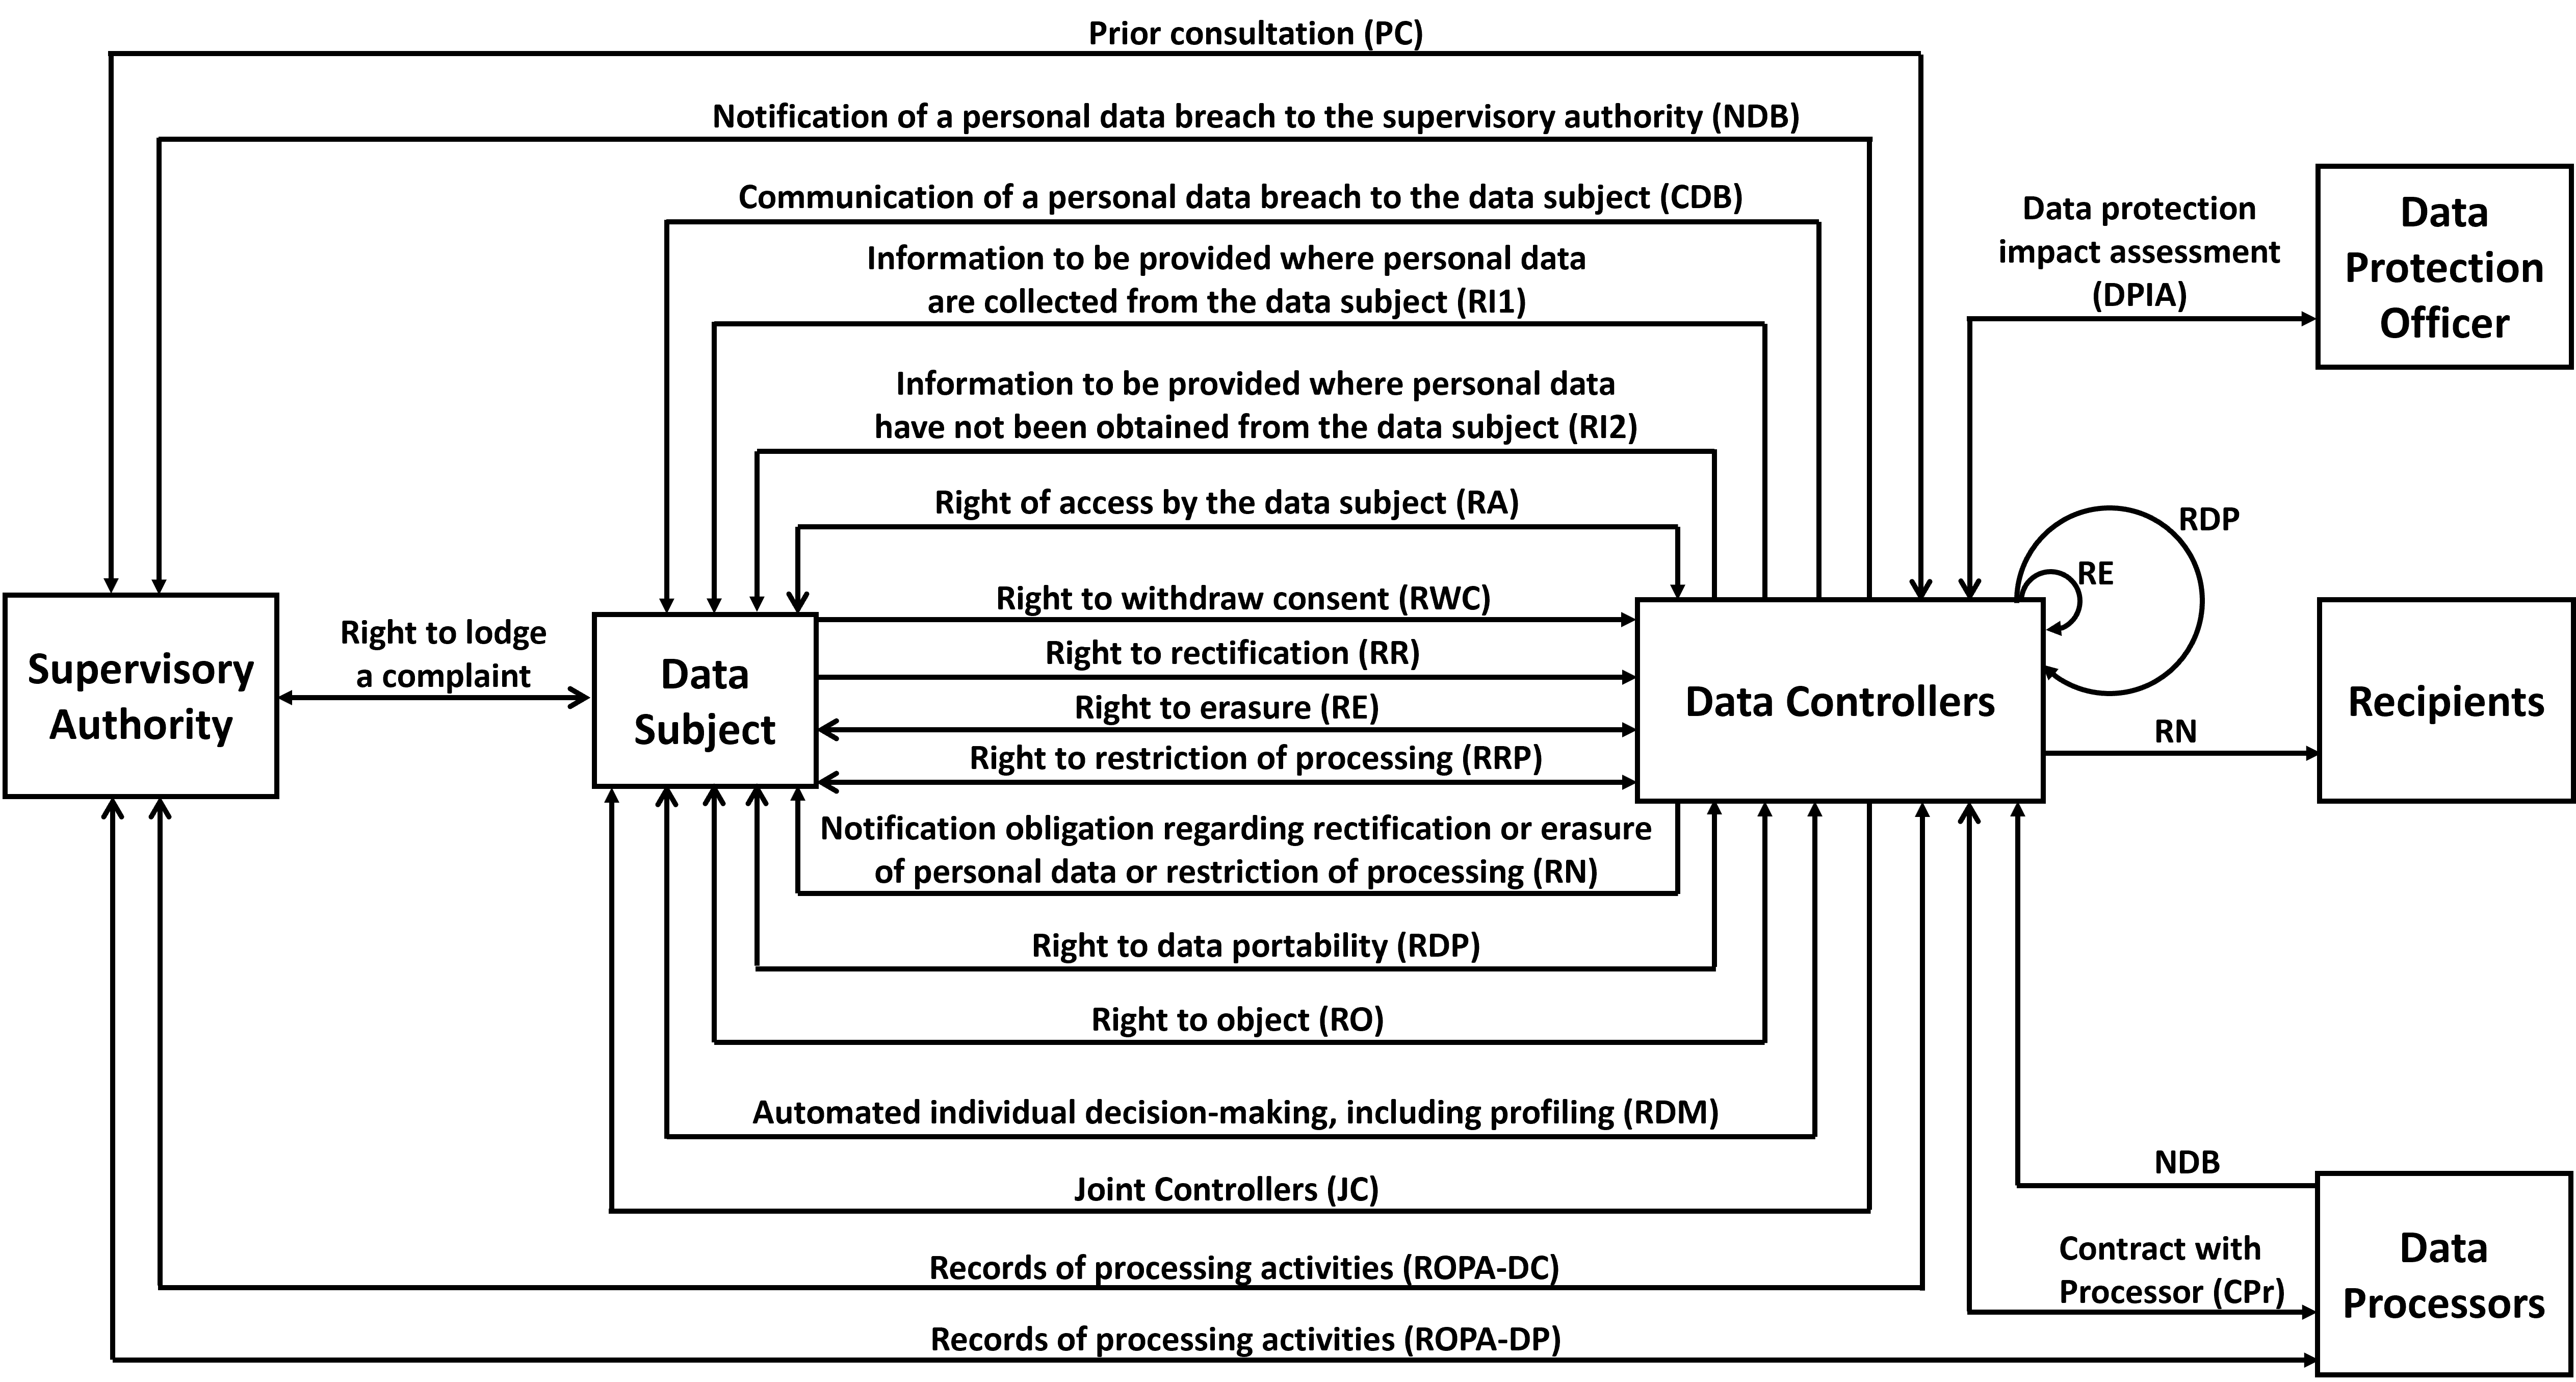
\includegraphics[width=\linewidth]{figures/chapter-1/information flow diagram.png}
    \caption[GDPR's rights and obligations as information flows.]{GDPR's rights and obligations as information flows. The bidirectional arrows represent a right or obligation in which a request for information and respective response is expected (the open arrowhead, \ding{220}, represents the entity waiting for the response, and the closed arrowhead, \ding{225}, the entity being requested). In contrast, the unidirectional arrows represent only a request or notification and no reply is expected (with the closed arrowhead, \ding{225}, representing the entity being requested or notified), adapted from~\cite{esteves_analysis_2022}.}
    \label{fig:gdpr_information_flows}
\end{figure}
\end{landscape}

\subsection{Personal data}
\label{sec:def_personal_data}

GDPR's Article 4.1~\citeyearpar{noauthor_regulation_2016} defines `personal data' as \textit{``any information relating to an identified or identifiable natural person''} such as \textit{``a name, an identification number, location data, an online identifier or to one or more factors specific to the physical, physiological, genetic, mental, economic, cultural or social identity of that natural person''}.
This Thesis relies on GDPR's definition of personal data and special categories of personal data.
In addition, it is also acknowledged that there are categories of data that are sensitive, even though they are not considered `special' under GDPR's Article 9.1, which might require additional consideration and/or protection, e.g., location data has the potential to reveal religious beliefs, sexual orientation or political opinions\footnote{DPV models \url{https://w3id.org/dpv\#SensitivePersonalData} as a subtype of \url{https://w3id.org/dpv\#PersonalData} and \url{https://w3id.org/dpv\#SpecialCategoryPersonalData} as a subtype of \url{https://w3id.org/dpv\#SensitivePersonalData}}.

Table \ref{tab:data_sensitivity}, derived from the analysis of~\cite{rumbold_what_2018}, illustrates data sensitivity for particular subcategories of data. For each data type, sensitivity is assessed from 0 to 10, i.e., from low to high sensitivity, and the relative frequency of falling into that particular sensitivity value, on a scale of 1 to 4, is also presented. For instance, data related to objects has a sensitivity of 0 and a frequency of 4 as it can not be used to identify a person, while occupation data would not be frequently classified as being highly sensitive, as demonstrated by the frequency value of 1 to the sensitivity value of 10.
In addition, data sensitivity assessment is highly contextual, as shown through the fact that the same data category can have a spectrum of sensitivity, e.g., anonymised data can have a low/high sensitivity if the risk of re-identification is very low/high, respectively. 
This evaluation of data sensitivity is also well aligned with GDPR's special categories of personal data, as can be seen through the last column of the table, where these special categories are identified and, indeed, the most sensitive are presented in Article 9, with the exception of social class data.

\begin{table}[ht]
\caption[Data sensitivity chart.]{Data sensitivity chart derived from~\cite{rumbold_what_2018}. GDPR's special categories of personal data are identified in the \textbf{GDPR} column.}
\label{tab:data_sensitivity}
\scriptsize
\centering
\begin{tabular}{|c|c||l|l|c|c|c|c|c|c|l|l|l||l|}
\multicolumn{2}{c}{} & \multicolumn{11}{c}{\textbf{DATA SENSITIVITY}} & \multicolumn{1}{c}{} \\
\hline
\multicolumn{2}{|c||}{\textbf{DATA TYPE}} & \multicolumn{1}{r|}{\cellcolor[HTML]{9A0000}{\color[HTML]{FFFFFF} 10}} & \multicolumn{1}{r|}{\cellcolor[HTML]{CB0000}{\color[HTML]{FFFFFF} 9}} & \multicolumn{1}{r|}{\cellcolor[HTML]{F56B00}{\color[HTML]{FFFFFF} 8}} & \multicolumn{1}{r|}{\cellcolor[HTML]{F8A102}7} & \multicolumn{1}{r|}{\cellcolor[HTML]{FFCB2F}6} & \multicolumn{1}{r|}{\cellcolor[HTML]{FFFE65}5} & \multicolumn{1}{r|}{\cellcolor[HTML]{D9EF8B}4} & \multicolumn{1}{r|}{\cellcolor[HTML]{A6D96A}{\color[HTML]{FFFFFF} 3}} & \multicolumn{1}{r|}{\cellcolor[HTML]{66BD63}{\color[HTML]{FFFFFF} 2}} & \multicolumn{1}{r|}{\cellcolor[HTML]{1A9850}{\color[HTML]{FFFFFF} 1}} & \multicolumn{1}{r||}{\cellcolor[HTML]{036400}{\color[HTML]{FFFFFF} 0}} & \textbf{GDPR} \\ \hline\hline
\multicolumn{1}{|c|}{} & Relating to objects & & & \multicolumn{1}{l|}{} & \multicolumn{1}{l|}{} & \multicolumn{1}{l|}{} & \multicolumn{1}{l|}{} & \multicolumn{1}{l|}{} & \multicolumn{1}{l|}{} & & & \multicolumn{1}{c||}{\cellcolor[HTML]{036400}{\color[HTML]{FFFFFF} \textbf{4}}} & \\ \cline{2-14}
\multicolumn{1}{|c|}{\multirow{-2}{*}{\textbf{\begin{tabular}[c]{@{}c@{}}Non-personal\\ data\end{tabular}}}} & \begin{tabular}[c]{@{}c@{}}Anonymised data\\ related to persons\end{tabular} & & & \cellcolor[HTML]{F56B00}{\color[HTML]{FFFFFF} \textbf{1}} & \cellcolor[HTML]{F8A102}\textbf{1} & \cellcolor[HTML]{FFCB2F}\textbf{1} & \cellcolor[HTML]{FFFE65}\textbf{1} & \cellcolor[HTML]{D9EF8B}\textbf{2} & \cellcolor[HTML]{A6D96A}{\color[HTML]{FFFFFF} \textbf{3}} & \multicolumn{1}{c|}{\cellcolor[HTML]{66BD63}{\color[HTML]{FFFFFF} \textbf{3}}} & \multicolumn{1}{c|}{\cellcolor[HTML]{1A9850}{\color[HTML]{FFFFFF} \textbf{4}}} & \multicolumn{1}{c||}{\cellcolor[HTML]{036400}{\color[HTML]{FFFFFF} \textbf{3}}} &                 \\ \hline\hline
\multicolumn{1}{|c|}{} & Opinions & & & \multicolumn{1}{l|}{} & \cellcolor[HTML]{F8A102}\textbf{3} & \cellcolor[HTML]{FFCB2F}\textbf{3} & \cellcolor[HTML]{FFFE65}\textbf{3} & \cellcolor[HTML]{D9EF8B}\textbf{3} & \cellcolor[HTML]{A6D96A}{\color[HTML]{FFFFFF} \textbf{3}} & \multicolumn{1}{c|}{\cellcolor[HTML]{66BD63}{\color[HTML]{FFFFFF} \textbf{3}}} & \multicolumn{1}{c|}{\cellcolor[HTML]{1A9850}{\color[HTML]{FFFFFF} \textbf{3}}} & & \\ \cline{2-14}
\multicolumn{1}{|c|}{} & Purchasing habits & & & \cellcolor[HTML]{F56B00}{\color[HTML]{FFFFFF} \textbf{1}} & \cellcolor[HTML]{F8A102}\textbf{2} & \cellcolor[HTML]{FFCB2F}\textbf{3} & \cellcolor[HTML]{FFFE65}\textbf{3} & \cellcolor[HTML]{D9EF8B}\textbf{3} & \cellcolor[HTML]{A6D96A}{\color[HTML]{FFFFFF} \textbf{3}} & \multicolumn{1}{c|}{\cellcolor[HTML]{66BD63}{\color[HTML]{FFFFFF} \textbf{3}}} & \multicolumn{1}{c|}{\cellcolor[HTML]{1A9850}{\color[HTML]{FFFFFF} \textbf{3}}} & & \\ \cline{2-14}
\multicolumn{1}{|c|}{} & Sex & & & \multicolumn{1}{l|}{} & \multicolumn{1}{l|}{} & \multicolumn{1}{l|}{} & \multicolumn{1}{l|}{} & \cellcolor[HTML]{D9EF8B}\textbf{3} & \cellcolor[HTML]{A6D96A}{\color[HTML]{FFFFFF} \textbf{3}} & \multicolumn{1}{c|}{\cellcolor[HTML]{66BD63}{\color[HTML]{FFFFFF} \textbf{3}}} & & & \\ \cline{2-14}
\multicolumn{1}{|c|}{} & Age & & & \multicolumn{1}{l|}{} & \cellcolor[HTML]{F8A102}\textbf{3} & \cellcolor[HTML]{FFCB2F}\textbf{3} & \cellcolor[HTML]{FFFE65}\textbf{3} & \cellcolor[HTML]{D9EF8B}\textbf{3} & \cellcolor[HTML]{A6D96A}{\color[HTML]{FFFFFF} \textbf{3}} & & & & \\ \cline{2-14}
\multicolumn{1}{|c|}{} & Income & & & \cellcolor[HTML]{F56B00}{\color[HTML]{FFFFFF} \textbf{2}} & \cellcolor[HTML]{F8A102}\textbf{3} & \cellcolor[HTML]{FFCB2F}\textbf{3} & \cellcolor[HTML]{FFFE65}\textbf{3} & \cellcolor[HTML]{D9EF8B}\textbf{3} & \cellcolor[HTML]{A6D96A}{\color[HTML]{FFFFFF} \textbf{3}} & & & & \\ \cline{2-14}
\multicolumn{1}{|c|}{} & Location & & \multicolumn{1}{c|}{\cellcolor[HTML]{CB0000}{\color[HTML]{FFFFFF} \textbf{1}}} & \cellcolor[HTML]{F56B00}{\color[HTML]{FFFFFF} \textbf{2}} & \cellcolor[HTML]{F8A102}\textbf{3} & \cellcolor[HTML]{FFCB2F}\textbf{3} & \cellcolor[HTML]{FFFE65}\textbf{3} & \cellcolor[HTML]{D9EF8B}\textbf{3} & \cellcolor[HTML]{A6D96A}{\color[HTML]{FFFFFF} \textbf{3}} & & & & \\ \cline{2-14}
\multicolumn{1}{|c|}{} & \begin{tabular}[c]{@{}c@{}}Lifestyle or\\ wellness data\end{tabular} & & \multicolumn{1}{c|}{\cellcolor[HTML]{CB0000}{\color[HTML]{FFFFFF} \textbf{3}}} & \cellcolor[HTML]{F56B00}{\color[HTML]{FFFFFF} \textbf{3}} & \cellcolor[HTML]{F8A102}\textbf{3} & \cellcolor[HTML]{FFCB2F}\textbf{3} & \cellcolor[HTML]{FFFE65}\textbf{3} & \cellcolor[HTML]{D9EF8B}\textbf{3} & \cellcolor[HTML]{A6D96A}{\color[HTML]{FFFFFF} \textbf{3}} & & & & \\ \cline{2-14}
\multicolumn{1}{|c|}{} & Occupation & \multicolumn{1}{c|}{\cellcolor[HTML]{9A0000}{\color[HTML]{FFFFFF} \textbf{1}}} & \multicolumn{1}{c|}{\cellcolor[HTML]{CB0000}{\color[HTML]{FFFFFF} \textbf{2}}} & \cellcolor[HTML]{F56B00}{\color[HTML]{FFFFFF} \textbf{3}} & \cellcolor[HTML]{F8A102}\textbf{3} & \cellcolor[HTML]{FFCB2F}\textbf{3} & \cellcolor[HTML]{FFFE65}\textbf{3} & \cellcolor[HTML]{D9EF8B}\textbf{3} & \cellcolor[HTML]{A6D96A}{\color[HTML]{FFFFFF} \textbf{3}} & & & & \\ \cline{2-14}
\multicolumn{1}{|c|}{} & Address & & & \cellcolor[HTML]{F56B00}{\color[HTML]{FFFFFF} \textbf{2}} & \cellcolor[HTML]{F8A102}\textbf{3} & \cellcolor[HTML]{FFCB2F}\textbf{3} & \cellcolor[HTML]{FFFE65}\textbf{3} & \cellcolor[HTML]{D9EF8B}\textbf{3} & \multicolumn{1}{l|}{} & & & & \\ \cline{2-14}
\multicolumn{1}{|c|}{} & Race & & & \cellcolor[HTML]{F56B00}{\color[HTML]{FFFFFF} \textbf{3}} & \cellcolor[HTML]{F8A102}\textbf{3} & \cellcolor[HTML]{FFCB2F}\textbf{3} & \cellcolor[HTML]{FFFE65}\textbf{3} & \cellcolor[HTML]{D9EF8B}\textbf{3} & \multicolumn{1}{l|}{} & & & & \textbf{Art. 9} \\ \cline{2-14}
\multicolumn{1}{|c|}{} & Ethnic group & & & \cellcolor[HTML]{F56B00}{\color[HTML]{FFFFFF} \textbf{3}} & \cellcolor[HTML]{F8A102}\textbf{3} & \cellcolor[HTML]{FFCB2F}\textbf{3} & \cellcolor[HTML]{FFFE65}\textbf{3} & \cellcolor[HTML]{D9EF8B}\textbf{3} & \multicolumn{1}{l|}{} & & & & \textbf{Art. 9} \\ \cline{2-14}
\multicolumn{1}{|c|}{} & \begin{tabular}[c]{@{}c@{}}Religious or\\ political beliefs\end{tabular} & & & \cellcolor[HTML]{F56B00}{\color[HTML]{FFFFFF} \textbf{3}} & \cellcolor[HTML]{F8A102}\textbf{3} & \cellcolor[HTML]{FFCB2F}\textbf{3} & \cellcolor[HTML]{FFFE65}\textbf{3} & \cellcolor[HTML]{D9EF8B}\textbf{3} & \multicolumn{1}{l|}{} & & & & \textbf{Art. 9} \\ \cline{2-14}
\multicolumn{1}{|c|}{} & Sexual orientation & & & \cellcolor[HTML]{F56B00}{\color[HTML]{FFFFFF} \textbf{3}} & \cellcolor[HTML]{F8A102}\textbf{3} & \cellcolor[HTML]{FFCB2F}\textbf{3} & \cellcolor[HTML]{FFFE65}\textbf{3} & \cellcolor[HTML]{D9EF8B}\textbf{3} & \multicolumn{1}{l|}{} & & & & \textbf{Art. 9} \\ \cline{2-14}
\multicolumn{1}{|c|}{} & Pregnancy & & \multicolumn{1}{c|}{\cellcolor[HTML]{CB0000}{\color[HTML]{FFFFFF} \textbf{3}}} & \cellcolor[HTML]{F56B00}{\color[HTML]{FFFFFF} \textbf{3}} & \cellcolor[HTML]{F8A102}\textbf{3} & \cellcolor[HTML]{FFCB2F}\textbf{3} & \cellcolor[HTML]{FFFE65}\textbf{3} & \cellcolor[HTML]{D9EF8B}\textbf{3} & \multicolumn{1}{l|}{} & & & & \textbf{Art. 9}  \\ \cline{2-14}
 & Transgender status & \multicolumn{1}{c|}{} & \multicolumn{1}{c|}{\cellcolor[HTML]{CB0000}{\color[HTML]{FFFFFF} \textbf{3}}} & \cellcolor[HTML]{F56B00}{\color[HTML]{FFFFFF} \textbf{3}} & \cellcolor[HTML]{F8A102}\textbf{3} & \cellcolor[HTML]{FFCB2F}\textbf{3} & \cellcolor[HTML]{FFFE65}\textbf{2} & \multicolumn{1}{l|}{} & \multicolumn{1}{l|}{} & & & & \textbf{Art. 9} \\ \cline{2-14}
\multicolumn{1}{|c|}{\multirow{-18}{*}{\textbf{\begin{tabular}[c]{@{}c@{}}Human \\ demographics, \\ behaviour,\\ thoughts \\ \& opinions\end{tabular}}}} & Social class & & & \cellcolor[HTML]{F56B00}{\color[HTML]{FFFFFF} \textbf{3}} & \cellcolor[HTML]{F8A102}\textbf{3} & \cellcolor[HTML]{FFCB2F}\textbf{3} & \multicolumn{1}{l|}{} & \multicolumn{1}{l|}{} & \multicolumn{1}{l|}{} & & & & \\ \cline{2-14} \hline\hline
\multicolumn{1}{|c|}{} & Facial images & \multicolumn{1}{c|}{} & \multicolumn{1}{c|}{} & & \cellcolor[HTML]{F8A102}\textbf{3} & \cellcolor[HTML]{FFCB2F}\textbf{3} & \cellcolor[HTML]{FFFE65}\textbf{3} & \cellcolor[HTML]{D9EF8B}\textbf{3} & \cellcolor[HTML]{A6D96A}{\color[HTML]{FFFFFF} \textbf{3}} & \multicolumn{1}{c|}{\cellcolor[HTML]{66BD63}{\color[HTML]{FFFFFF} \textbf{2}}} & & & \textbf{Art. 9} \\ \cline{2-14}
\multicolumn{1}{|c|}{} & Body images & & \multicolumn{1}{c|}{\cellcolor[HTML]{CB0000}{\color[HTML]{FFFFFF} \textbf{3}}} & \cellcolor[HTML]{F56B00}{\color[HTML]{FFFFFF} \textbf{3}} & \cellcolor[HTML]{F8A102}\textbf{3} & \cellcolor[HTML]{FFCB2F}\textbf{3} & \cellcolor[HTML]{FFFE65}\textbf{3} & \cellcolor[HTML]{D9EF8B}\textbf{3} & \cellcolor[HTML]{A6D96A}{\color[HTML]{FFFFFF} \textbf{3}} & \multicolumn{1}{c|}{\cellcolor[HTML]{66BD63}{\color[HTML]{FFFFFF} \textbf{2}}} & & & \textbf{Art. 9} \\ \cline{2-14}
\multicolumn{1}{|c|}{\multirow{-3}{*}{\textbf{\begin{tabular}[c]{@{}c@{}}Biometrics\end{tabular}}}} & \begin{tabular}[c]{@{}c@{}}Any traits processed\\ for biometrics\end{tabular} & & \multicolumn{1}{c|}{\cellcolor[HTML]{CB0000}{\color[HTML]{FFFFFF} \textbf{3}}} & \cellcolor[HTML]{F56B00}{\color[HTML]{FFFFFF} \textbf{3}} & \cellcolor[HTML]{F8A102}\textbf{3} & \multicolumn{1}{l|}{} & \multicolumn{1}{l|}{} & \multicolumn{1}{l|}{} & \multicolumn{1}{l|}{} & & & & \textbf{Art. 9} \\ \hline\hline
\multicolumn{1}{|c|}{} & Diagnoses & & \multicolumn{1}{c|}{\cellcolor[HTML]{CB0000}{\color[HTML]{FFFFFF} \textbf{3}}} & \cellcolor[HTML]{F56B00}{\color[HTML]{FFFFFF} \textbf{3}} & \cellcolor[HTML]{F8A102}\textbf{3} & \cellcolor[HTML]{FFCB2F}\textbf{3} & \multicolumn{1}{l|}{} & \multicolumn{1}{l|}{} & \multicolumn{1}{l|}{} & & & & \textbf{Art. 9} \\ \cline{2-14}
\multicolumn{1}{|c|}{} & Genetic data & \multicolumn{1}{c|}{\cellcolor[HTML]{9A0000}{\color[HTML]{FFFFFF} \textbf{3}}} & \multicolumn{1}{c|}{\cellcolor[HTML]{CB0000}{\color[HTML]{FFFFFF} \textbf{3}}} & \cellcolor[HTML]{F56B00}{\color[HTML]{FFFFFF} \textbf{4}} & \cellcolor[HTML]{F8A102}\textbf{3} & \cellcolor[HTML]{FFCB2F}\textbf{3} & \multicolumn{1}{l|}{} & \multicolumn{1}{l|}{} & \multicolumn{1}{l|}{} & & & & \textbf{Art. 9} \\ \cline{2-14}
\multicolumn{1}{|c|}{\multirow{-3}{*}{\textbf{\begin{tabular}[c]{@{}c@{}}Medical or \\ health data\end{tabular}}}} & \begin{tabular}[c]{@{}c@{}}Highly sensitive\\ diagnoses\end{tabular} & \multicolumn{1}{c|}{\cellcolor[HTML]{9A0000}{\color[HTML]{FFFFFF} \textbf{4}}} & \multicolumn{1}{c|}{\cellcolor[HTML]{CB0000}{\color[HTML]{FFFFFF} \textbf{3}}} & \multicolumn{1}{l|}{} & \multicolumn{1}{l|}{} & \multicolumn{1}{l|}{} & \multicolumn{1}{l|}{} & \multicolumn{1}{l|}{} & \multicolumn{1}{l|}{} & & & & \textbf{Art. 9} \\ \hline
\end{tabular}
\end{table}

\subsection{Decentralised data environments}
\label{sec:def_decentralised_env}

A decentralised environment for data represents a significant paradigm shift in relation to the current status of digital data management.
The Web we have today is a centralised Web where data is kept in data silos, controlled only by a handful of Big Tech players, while in a decentralised Web approach \textit{people choose where they store their data} and \textit{exert control over whom gets access to which parts of their data}~\citep{verborgh_paradigm_2017}.

Figure \ref{fig:decentralisation} illustrates the distinction between these two paradigms.
In a centralised setting, data and applications are coupled and data is kept in \textit{`walled gardens'} controlled by the entities behind centralised platforms such as Facebook, Twitter, or LinkedIn, leaving users without the possibility of reusing it elsewhere~\citeyearpar{noauthor_break_2008}.
By shifting to a decentralised Web, users are able to choose where their data is stored and are in control of their identity, while applications are detached from data, becoming \textit{``views''} over it and fostering innovation and competition through separate markets for data and services~\citep{verborgh_re-decentralizing_2022}.
Modern decentralised environments include Internet of Things (IoT) ecosystems or personal datastores (\ref{sec:def_pds}).

\begin{figure}[ht]
    \centering
    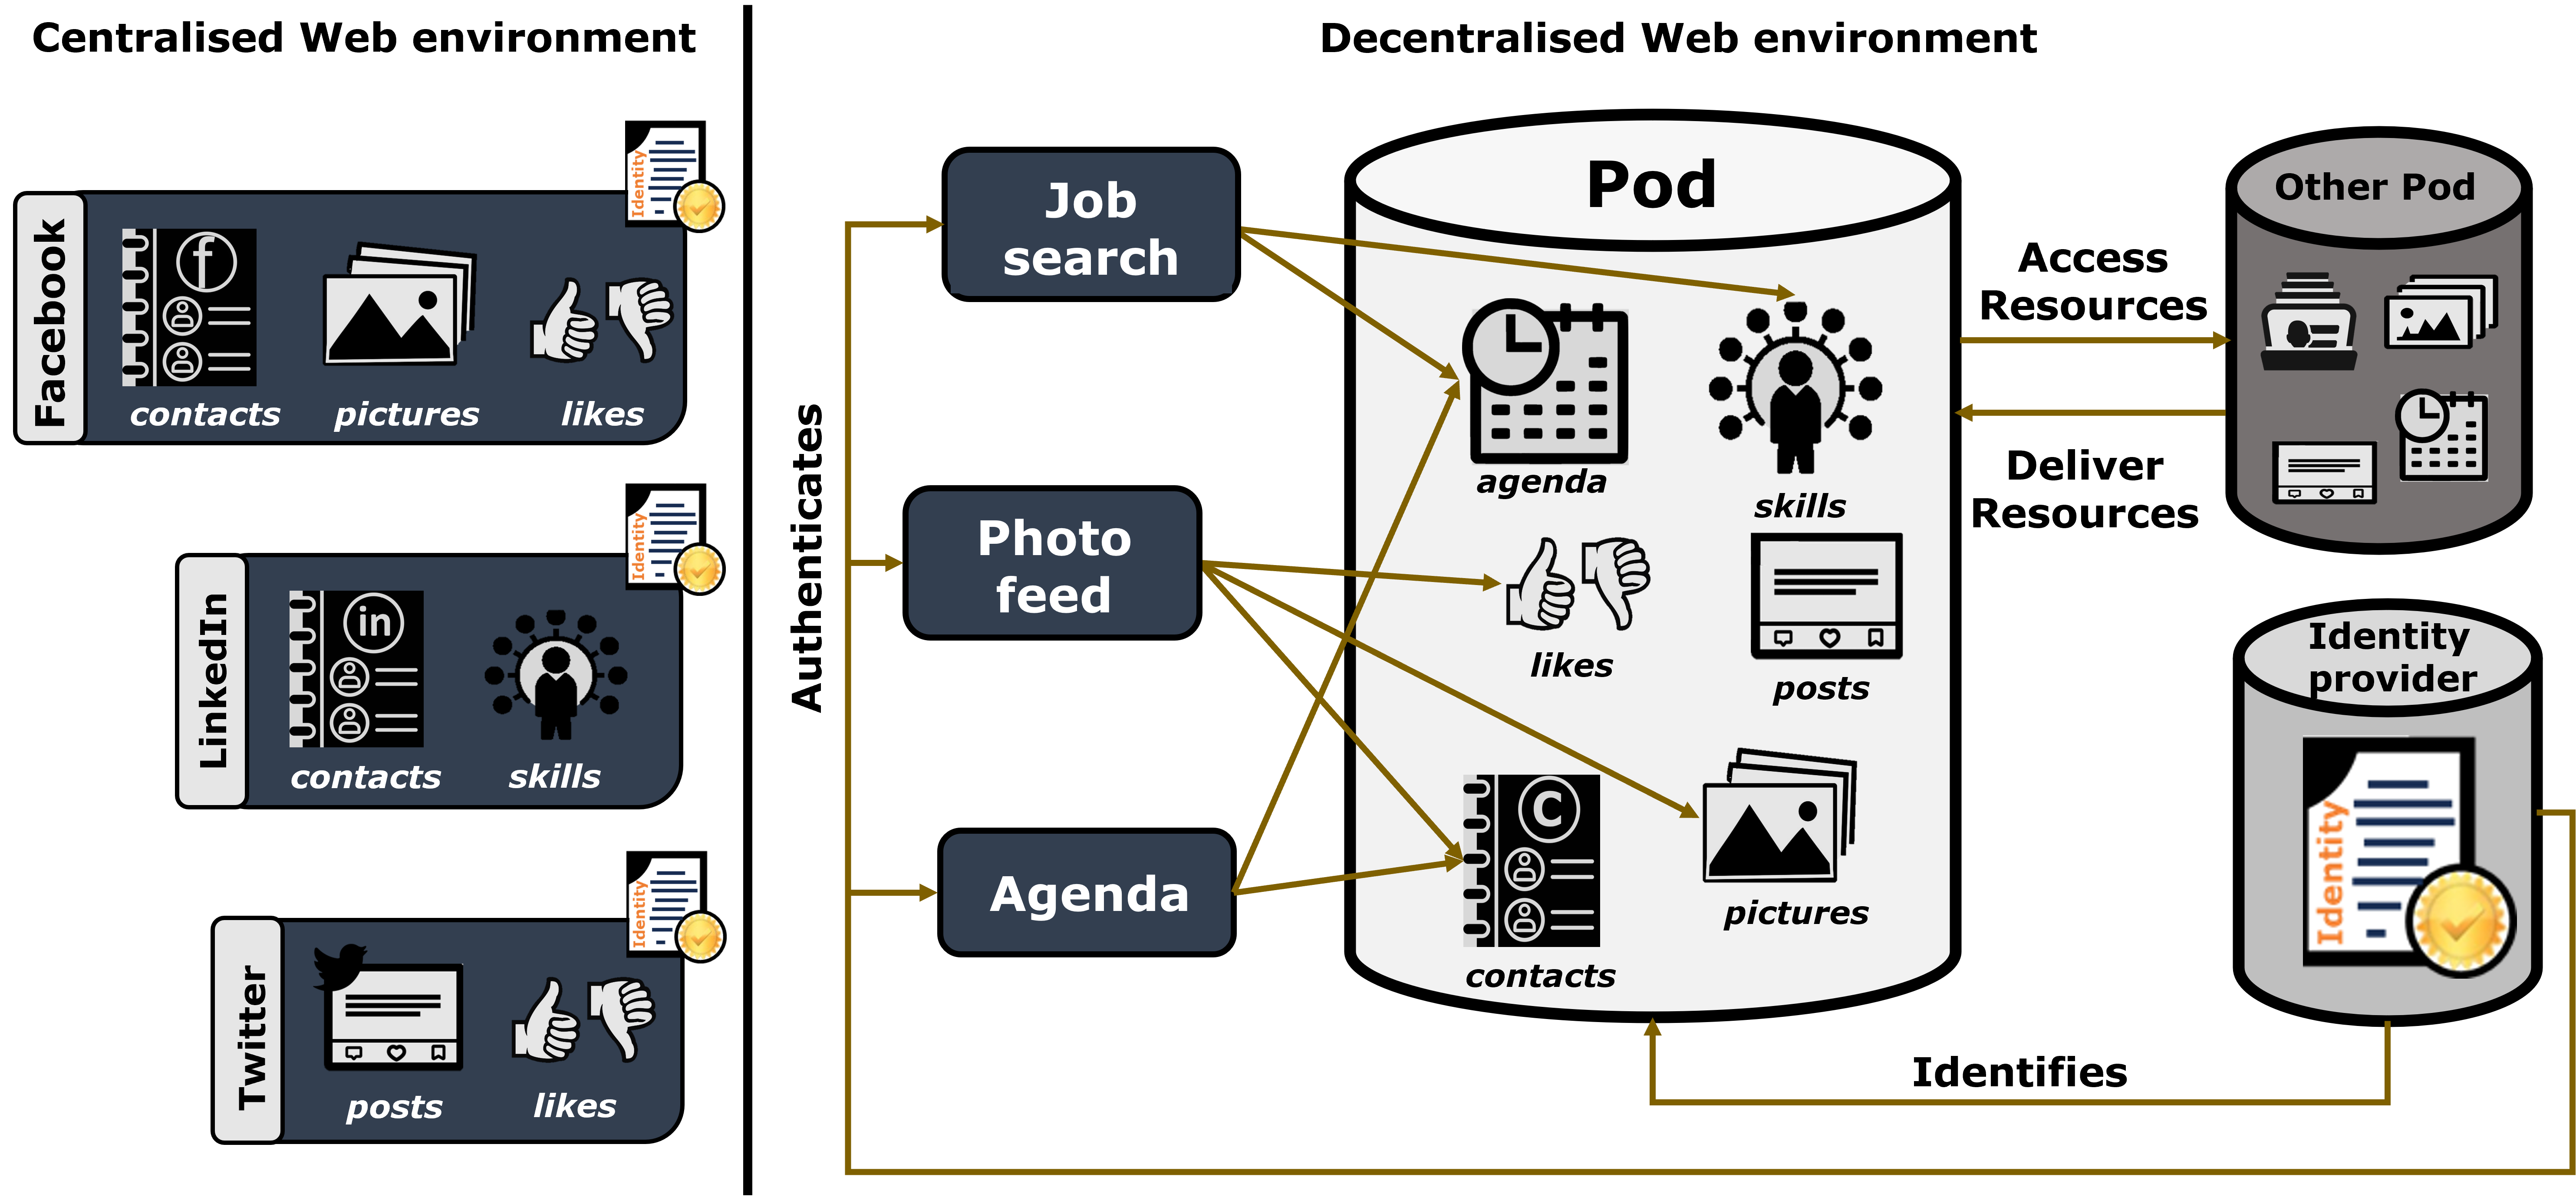
\includegraphics[width=\linewidth]{figures/chapter-1/decentralisation.png}
    \caption{Distinction between centralised and decentralised data environments.}
    \label{fig:decentralisation}
\end{figure}

This Thesis focuses on providing users with the tools to better determine access to personal data resources stored in decentralised settings, according to EU law on personal data protection.
Beyond access control (\ref{sec:def_access_control}), usage control solutions also need to be developed to provide data subjects with \textit{``control over data usage once access to the data has been granted''}~\citep{akaichi_semantic_2022}.

\subsubsection{Personal datastores}
\label{sec:def_pds}

In its \textit{TechDispatch \#3/2020}~\citep{european_data_protection_supervisor_techdispatch_2021}, the EDPS envisioned the development of personal data spaces, managed through Personal Information Management Systems (PIMS) as a mechanism to enable personal data sovereignty where \textit{``Individuals, service providers and applications would need to authenticate to access a personal storage centre''} and individuals are able to \textit{``customize what categories of data they want to share and with whom''} while keeping a record of \textit{``who has had access to their digital behaviour''} and enabling data portability and interoperability.

Such decentralised systems (\ref{sec:def_decentralised_env}) allow data subjects to directly determine who has access to their data, and under which conditions, and can actually play an important role in facilitating the exercise of data subjects’ rights, including the rights of access, erasure, and data portability or the right to withdraw consent~\citep{janssen_personal_2020}.
In the last few years, different personal datastores initiatives have been gaining prominence and adoption, including the Solid project\footnote{\url{https://solidproject.org/} (accessed on 15 March 2024)}~\citep{fallatah_personal_2023}, which is the adopted use case for the research in this Thesis.

Solid is a free, open-source initiative that delivers on the promise of decentralising the storage of data by relying on Web standards and on Semantic Web vocabularies to promote data and services interoperability. To fulfil this vision, the Solid specification relies on authentication and authorisation protocols to provide private, secure, and granular access to data stored in Solid's personal online datastores, the so-called `Pods'~\citep{mansour_demonstration_2016}.

Moreover, beyond personal datastores, decentralised initiatives at the community level are also being proposed.
For instance, data cooperative\footnote{Data infrastructure formed through the voluntary and collaborative pooling efforts of individuals.} infrastructures still give their members decision-making control over their data, while allowing them to get paid to share their data in an environment where they have more decision power than what they would have on their own or in other types of data-sharing environments~\citep{mechant_saving_2021}.
These community-level stores are also starting to be regulated, e.g., by the DGA~\citeyearpar{noauthor_regulation_2022}.
\section{Publications}
\label{sec:publications}

The following Sections list the works published and presented during the accomplishment of this Thesis. When identified with a $^{\dagger}$, the authors contributed equally to the publication work.

In addition, Figure \ref{fig:timeline} illustrates the timeline of publications, presentations, and research stays of this Thesis.

% TODO: Tas 5 in the figure -- update to start mid-2022
\begin{figure}
    \centering
    \includegraphics[width=\linewidth]{figures/chapter-1/timeline.png}
    \caption{Timeline of publications, presentations, and research stays of this Thesis.}
    \label{fig:timeline}
\end{figure}

\subsection{Journal contributions}
\label{sec:publications_journal}

\begin{enumerate}
    \item [(PJ1)] Analysis of Ontologies and Policy Languages to Represent Information Flows in GDPR. (2022) \textbf{B. Esteves}, V. Rodríguez-Doncel. \textit{Semantic Web Journal}, pp. 1--35. % TODO: update when SWJ issue is published
    \item [(PJ2)] ``Who Should I Trust with My Data?'' Ethical and Legal Challenges for Innovation in New Decentralized Data Management Technologies. (2023) H. Asgarinia$^{\dagger}$, A. Chomczyk Penedo$^{\dagger}$, \textbf{B. Esteves}$^{\dagger}$, D. Lewis. \textit{Information 14(7)}, \url{https://doi.org/10.3390/info14070351}.
    \item [(PJ3)] Is Automated Consent in Solid GDPR-Compliant? An Approach for Obtaining Valid Consent with the Solid Protocol. (2023) M. Florea$^{\dagger}$, \textbf{B. Esteves}$^{\dagger}$. \textit{Information 14(12), Special Issue on Addressing Privacy and Data Protection in New Technological Trends}, \url{https://doi.org/10.3390/info14120631}.
    \item [(PJ4)] Enhancing Data Use Ontology (DUO) for Health-Data Sharing by Extending it with ODRL and DPV. (2023) H. J. Pandit$^{\dagger}$, \textbf{B. Esteves}$^{\dagger}$.  \textit{Accepted to be published at the Semantic Web Journal}. % TODO: update when SWJ issue is published
\end{enumerate}

\subsection{Conference contributions}
\label{sec:publications_conference}

\begin{enumerate}
    \item [(PC1)] Extracting and Understanding Call-to-actions of Push-Notifications. (2022) \textbf{B. Esteves}, K. Fraser, S. Kulkarni, O. Conlan, V. Rodríguez-Doncel.  In \textit{Natural Language Processing and Information Systems. Edited by P. Rosso, V. Basile, R. Martínez, E. Métais, F. Meziane, Volume 13286}, pp. 147-–159. Springer International Publishing. \url{https://doi.org/10.1007/978-3-031-08473-7\_14}.
    \item [(PC2)] Now, Later, Never: A Study of Urgency in Mobile Push-Notifications. (2022) \textbf{B. Esteves}, K. Fraser, S. Kulkarni, O. Conlan, V. Rodríguez-Doncel. In \textit{Advances in Mobile Computing and Multimedia Intelligence. Edited by P. Delir Haghighi, I. Khalil, G. Kotsis}, pp. 38-–44. Springer Nature Switzerland. \url{https://doi.org/10.1007/978-3-031-20436-4\_4}.
    \item [(PC3)] Automating the Response to GDPR’s Right of Access. (2022) \textbf{B. Esteves}, V. Rodríguez-Doncel, R. Longares. In \textit{Legal Knowledge and Information Systems}, pp. 170–-175. IOS Press. \url{https://doi.org/10.3233/FAIA220462}.
    \item [(PC4)] Semantics for Implementing Data Reuse and Altruism Under EU’s Data Governance Act. (2023) \textbf{B. Esteves}, V. Rodríguez-Doncel,  H. J. Pandit, D. Lewis. In \textit{Knowledge Graphs: Semantics, Machine Learning, and Languages. Edited by M. Acosta et al.}, pp. 210--226. IOS Press. \url{https://doi.org/10.3233/SSW230015}.
\end{enumerate}

\subsection{Workshop contributions}
\label{sec:publications_workshop}

\begin{enumerate}
    \item [(PW1)] Challenges in the Digital Representation of Privacy Terms. (2021) \textbf{B. Esteves}. In \textit{AI Approaches to the Complexity of Legal Systems XI-XII. Edited by V. Rodríguez-Doncel, M. Palmirani, M. Araszkiewicz, P. Casanovas, U. Pagallo, G. Sartor, Volume 13048}, pp. 313–-327. Springer International Publishing. \url{https://doi.org/10.1007/978-3-030-89811-3\_22}.
    \item [(PW2)] ODRL Profile for Expressing Consent through Granular Access Control Policies in Solid. (2021) \textbf{B. Esteves}, H. J. Pandit, V. Rodríguez-Doncel. In \textit{2021 IEEE European Symposium on Security and Privacy Workshops (EuroS\&PW)}, pp. 298-–306. \url{https://doi.org/10.1109/EuroSPW54576.2021.00038}
    \item [(PW3)] Using the ODRL Profile for Access Control for Solid Pod Resource Governance. (2022) \textbf{B. Esteves}, V. Rodríguez-Doncel, H. J. Pandit, N. Mondada, P. McBennett. In \textit{The Semantic Web: ESWC 2022 Satellite Events. Edited by P. Groth, A. Rula, J. Schneider, I. Tiddi, E. Simperl, P. Alexopoulos, R. Hoekstra, M. Alam, A. Dimou, M. Tamper}, pp. 16-–20. Springer International Publishing. \url{https://doi.org/10.1007/978-3-031-11609-4\_3}
    \item [(PW4)] Semantifying the Governance of Data in Europe. (2022) \textbf{B. Esteves}, V. Rodríguez-Doncel. In \textit{18th International Conference on Semantic Systems - CEUR Workshop Proceedings, Volume 3235}. \url{https://ceur-ws.org/Vol-3235/paper17.pdf}.
    \item [(PW5)] Fostering trust with transparency in the data economy era: An integrated ethical, legal, and knowledge engineering approach. (2022) \textbf{B. Esteves}, H. Asgarinia, A. Chomczyk Penedo, B. Mutiro, D. Lewis. In \textit{Proceedings of the 1st International Workshop on Data Economy}, pp. 57-–63. \url{https://doi.org/10.1145/3565011.3569061}.
    \item [(PW6)] Towards an Architecture for Data Altruism in Solid. (2023) \textbf{B. Esteves}. In \textit{22nd International Semantic Web Conference: Posters, Demos, and Industry Tracks}. (Accepted for publication)
    \item [(PW7)] Using Patterns to Manage Governance of Solid Apps. (2023) \textbf{B. Esteves}, H. J. Pandit. In \textit{14th Workshop on Ontology Design and Patterns (WOP 2023@ISWC 2023)}. (Accepted for publication)
\end{enumerate}

\subsection{Oral presentations}
\label{sec:oral_presentations}

The following presentations were given during the realisation of this Thesis.

% TODO: create post with oral presentations with links to abstracts and slides of presentations in Zenodo}

\begin{enumerate}
    \item [(OP1)] Can privacy terms be negotiated in Solid's personal datastores? \textbf{B. Esteves}. Short talk at the \textit{2021 IEEE Symposium and Workshops on Security \& Privacy} (26/May/2021).
    \item [(OP2)] `Who should I trust with my data?': are decentralised technologies the answer to achieving ethical and lawful data governance practices? H. Asgarinia, A. Chomczyk Penedo, \textbf{B. Esteves}, D. Lewis, B. Mutiro. Presentation at the \textit{Data and the Common Workshop 2022} (04/March/2022).
    \item [(OP3)] Access control policies for Solid. \textbf{B. Esteves}. Demonstration at the \textit{2022 COST EU Workshop on Privacy Issues in Distributed Social Knowledge Graphs} (14/June/2022).
    \item [(OP4)] Establishing Data (Re-)Use Agreements Through Semantic Policies for Legally-aware Data Sharing. \textbf{B. Esteves}. Lightning talk at the \textit{SEMIC Conference 2022} (06/December/2022).
    \item [(OP5)] Altruistic (Re-)Use of Health Data through Semantic Policies. \textbf{B. Esteves}. Short talk at the \textit{2nd DPSN International Data Protection Day} (27/January/2023).
    \item [(OP6)] Privacy Receipts in Solid Pods. \textbf{B. Esteves}, J. Lindquist. Presentation at the \textit{2023 COST EU Workshop on Privacy Issues in Distributed Social Knowledge Graphs} (13/February/2023).
    \item [(OP7)] Policies in Solid: The Road Ahead. \textbf{B. Esteves}. Presentation at the \textit{Solid Symposium 2023} (31/March/2023).
    \item [(OP8)] Enhancing Solid with Legally-aware Policies. \textbf{B. Esteves}. Presentation at the \textit{Governing Artificial Intelligence International Symposium 2023} (23/May/2023).
\end{enumerate}
\section{Projects}
\label{sec:projects}

The following projects funded the work presented in this Thesis:

\paragraph{PROTECT ITN:} Protecting Personal Data Amidst Big Data Innovation (PROTECT) is an EU-funded Innovative Training Network project with the goal of developing \textit{``new ways of empowering users of digital services to understand the risks they take when they go online and to offer new ways to enable companies to incorporate data protection into digital services''} and train \textit{``a new generation of 14 early stage researchers who will integrate and apply arguments, analyses and tools from across the fields of law, ethics and knowledge engineering''}\footnote{Extracted from \url{https://cordis.europa.eu/project/id/813497} (accessed on 15 March 2024).}. This project has received funding from the European Union’s Horizon 2020 research and innovation programme under the Marie Skłodowska-Curie grant agreement No. 813497.

\paragraph{AURORA:} Achieving a new European Energy Awareness (AURORA) is an EU-funded Innovation Action project whose main objective is to \textit{``empower several thousand citizens across five locations in Denmark, England, Portugal, Slovenia, and Spain to make more informed energy decisions''}\footnote{Extracted from \url{https://cordis.europa.eu/project/id/101036418} (accessed on 15 March 2024).}. This project has received funding from the European Union’s Horizon 2020 research and innovation programme under grant agreement No. 101036418.

\paragraph{INESData:} Infraestructura para la Investigación de Espacios de Datos (INESData) is an EU-funded project with the main goal of creating and installing a data governance structure and technological components for common data spaces. This project has received funding from the European Union’s NextGenerationEU funding programme.

\paragraph{COST DKG:} COST Action on Distributed Knowledge Graphs (DKG), with grant agreement No. CA19134, whose main goal is to \textit{``create a research community for deployable Distributed Knowledge Graph technologies that are standards-based, and open, embrace the FAIR principles, allow for access control and privacy protection, and enable the decentralised publishing of high quality data''}\footnote{Extracted from \url{https://www.cost.eu/actions/CA19134/} (accessed on 15 March 2024).}.
\section{Research stays}
\label{sec:research_stays}

The research stays done in the context of this Thesis are outlined below.

\paragraph{01/10/2021 -- 01/12/2021 (2 months):} Research stay at \textit{EmPushy, Dublin, Ireland}\footnote{\url{https://www.empushy.com/} (accessed on 15 March 2024)}, supervised by Dr. Kieran Fraser. During this stay, the Annotation of Push-Notifications (APN) ontology was created to annotate push-notification datasets and train models to identify the presence of personal data in notifications' text, the intent of the notification, its persuasiveness, and so on. As this ontology is out of the scope of this Thesis, its description is omitted from this document. This work resulted in the publication of two conference papers, (PC1) and (PC2)~(\cite{esteves_extracting_2022, esteves_now_2022}, respectively). An analysis of which data to track in EmPushy's tools, and respective GDPR requirements to fulfil, was also performed with the EmPushy team. This stay was funded by the PROTECT ITN.

\paragraph{01/02/2022 -- 31/07/2022 (6 months -- half-time):} Virtual research stay at \textit{Inrupt, Inc., Boston, United States of America}\footnote{\url{https://www.inrupt.com/} (accessed on 15 March 2024)}, supervised by Pat McBennett and Nicolas Mondada. During this stay, an overview of relevant vocabularies related to the Solid ecosystem was performed. Moreover, this Thesis work on the ODRL profile for Access Control (OAC) was improved with the requirements brought by Inrupt's use cases and a Solid application (Solid ODRL access control Policies Editor -- SOPE) was developed to generate and store OAC policies in Solid Pods. This work resulted in the publication of the (PW3) workshop paper~\citep{esteves_using_2022}. This stay was funded by the PROTECT ITN.

\paragraph{01/09/2022 -- 01/12/2022 (3 months):} Research stay at \textit{ADAPT Centre, Trinity College Dublin, Dublin, Ireland}\footnote{\url{https://www.adaptcentre.ie/} (accessed on 15 March 2024)}, supervised by Prof. Dr. Harshvardhan J. Pandit and Prof. Dr. Dave Lewis. During this stay, the Policy LAnguage for Solid’s Metadata-based Access control (PLASMA) was developed. We also contributed to the development of the Data Privacy Vocabulary (DPV) specifications, including writing documentation and use cases, in particular, related to the exercising of data subjects' rights and the new DGA law. This work resulted in the publication of one conference and two workshop papers, (PC4), (PW6), and (PW7) (\cite{esteves_semantics_2023}, \cite{esteves_towards_2023} and \cite{esteves_using_2023}, respectively). This stay was funded by the PROTECT ITN.

\paragraph{01/03/2023 -- 18/03/2023 (~3 weeks):} Short-Term Scientific Mission at \textit{KNoWS, IDLab, Ghent University, Ghent, Belgium}\footnote{\url{https://knows.idlab.ugent.be/} (accessed on 15 March 2024)}, supervised by Prof. Dr. Ruben Verborgh. The main objective of this stay was to discuss and establish technical and legal requirements to align Solid with data protection principles and understand current issues and solutions that need to be dealt with and reused to implement such requirements in decentralised data-sharing environments. This mission was funded by the DKG COST Action.

\chapter{State of the Art}
\label{chap:sota}

\begin{tcolorbox}[colback=royallavender!40]
The content of this Chapter has already been partially included in the articles published during this Thesis~\citep{esteves_odrl_2021,esteves_analysis_2022,asgarinia_who_2023,esteves_using_2023,florea_is_2023}.
\end{tcolorbox}

This Chapter presents the state of the art on the representation of policies and personal data processing metadata in the context of determining access to decentralised personal data systems, focusing on solutions that use Semantic Web technologies and cater to data protection law requirements.
Since there are different areas being covered in this state of the art analysis, each topic will be first introduced with a list of criteria used to perform said analysis.
The prefixes and namespaces used in the Listings in this Chapter are explicitly defined in the \hyperref[sec:namespaces]{Namespaces list}.

Thus, a literature review was performed in the subsequent areas, following the methodology described in Section~\ref{sec:technical_review}:

\begin{itemize}
    \item [\textbf{\ref{sec:sota_solid}}] Decentralising the access to personal data with Solid
    \item [\textbf{\ref{sec:sota_vocabularies}}] Representing personal data processing information
    \item [\textbf{\ref{sec:sota_policies}}] Using policy languages to specify access control conditions
\end{itemize}

Through this analysis, a series of gaps and challenges in the representation of privacy terms was identified, in order to have a legally-aligned Solid environment, and is described in Section~\ref{sec:challenges}.

\section{Decentralising the access to personal data with Solid}
\label{sec:sota_solid}

As attested in Section~\ref{sec:def_decentralised_env}, current efforts are underway to decentralise today's Web. By decoupling data from applications, Web users will have their data stored in an environment they can control and can choose what data they want to make publicly accessible or accessible only to certain users while using their application of choice to manage said data.
This represents a significant paradigm shift regarding users' current online experience -- instead of being locked away in Big Tech companies' storage servers, data can be stored on individual personal datastores maintained by a provider chosen by the user or hosted by the user itself on its private server.
In this context, the Solid project~\citep{sambra_solid_2016,mansour_demonstration_2016} has been gaining prominence as it relies on Web standards to achieve this degree of decentralisation -- its ultimate goal is to give Web users a personal datastore, i.e., a Pod, per user, with a granular access control system managed by the user, which they can use to select which people and/or applications have access to the resources stored on their Pod.
As such, with Solid, applications and the companies behind them do not store the (personal) data of their users, acting only as interfaces that can read, write, or append data to/from Pods.
Such an ecosystem \textit{``fosters innovation and competition through separate markets for data and applications''}~\citep{verborgh_paradigm_2017}, while allowing Web users to exert a degree of control over their data that is currently impossible to wield.

In particular, the Solid protocol~\citep{capadisli_solid_2022} describes how servers and apps should behave by relying on the following Web standards:

\begin{itemize}
    \item HTTP~\citep{fielding_http_2022} -- The Hypertext Transfer Protocol describes an architecture and semantics for \textit{``distributed, collaborative, hypertext information systems''} to share data.
    \item RDF~\citep{cyganiak_rdf_2014} -- The Resource Description Framework defines a data model to represent information in the Web, including a schema~\citep{brickley_rdf_2014} and serialisation syntaxes for storing and exchanging RDF such as Turtle~\citep{prudhommeaux_rdf_2014} and JSON-LD~\citep{gregg_kellogg_json-ld_2020}.
    \item LDP~\citep{speicher_linked_2015} -- The Linked Data Platform specification expresses how to use \textit{``HTTP for accessing, updating, creating and deleting resources from servers that expose their resources as Linked Data''}.
    \item SPARQL~\citep{harris_sparql_2013} -- The SPARQL language can be used to query RDF databases. %Solid also uses a subset of SPARQL UPDATE through HTTP PATCH queries.
    \item WebID-TLS~\citep{story_webid-tls_2014} -- A protocol that uses WebIDs to authenticate users on the Web.
    \item OIDC~\citep{sakimura_openid_2014} -- The OpenID Connect standard is an authentication protocol to assert the user's identity. 
\end{itemize}

Moreover, Table \ref{tab:definitions} provides an overview of Solid-related concepts, their definitions, and corresponding classes and properties already modelled in Solid-related vocabularies.
The authentication and authorisation protocols compose Solid's two main building blocks -- an up-to-date list of Solid specifications, including technical reports for both aforementioned building blocks, is maintained by the Solid Community Group at \url{https://solidproject.org/TR/}.
Authentication is a necessary feature to identify users when they want to log into their Pod and/or when they want to use an app to perform a certain action over resources stored in their Pod.
Thus, Solid's authentication protocol uses Solid's WebID specification to identify agents through URIs, as specified in Table~\ref{tab:definitions}, which when dereferenced return a WebID profile document that should include information regarding the identity provider chosen by the Solid user and the Pod storage location and may include information regarding an available inbox where users and applications can leave messages to the user~\citep{balseiro_solid_2022}.
In addition, to verify the identity of agents, the Solid Protocol recommends the usage of the Solid OIDC protocol\footnote{A Solid-OIDC Primer~\citep{morgan_oidcprimer_2022} is also being developed to provide additional knowledge on Solid OIDC's authentication flows.}~\citep{coburn_oidc_2022}, however additional authentication methods, such as the previously mentioned WebID-TLS, can also be implemented.

The authorisation protocol specifies mechanisms used by Solid servers to reply to requests of particular users or apps to have access to certain resources, containers of resources, or even to the whole Pod.
Furthermore, the Solid protocol states that a Solid server \textit{``MUST conform to either or both Web Access Control (WAC) and Access Control Policy (ACP) specifications''} in order for it to be a compliant Solid server.
Specific authorisation use cases and requirements are documented by the~\cite{solid_editorial_team_use_2023} and further details on the authorisation methods will be given in Section~\ref{sec:sota_solid_access_control}.
In addition to the authorisation specifications, there is a third protocol being developed to ensure data interoperability and (re)usability across Pod providers, agents, and applications -- the Solid Application Interoperability (SAI) specification~\citep{bingham_interop_2023}.

\begin{landscape}
\begin{table}[p]
\caption[Overview of Solid-related concepts.]{Overview of Solid-related concepts, their definitions, and related terms modelled on Solid specifications.}
\label{tab:definitions}
\begin{tabular}{c||l|c}
\textbf{Concept} & \textbf{Definition} & \textbf{Solid vocabularies} \\ \hline\hline
Pod & A personal datastore that conforms to the Solid protocol & \texttt{pim:Storage} \\ \hline
Resource & \begin{tabular}[c]{@{}l@{}}Target asset stored in a Pod identified by a URI. Container resources can\\ contain other resources including containers\end{tabular} & \begin{tabular}[c]{@{}c@{}}\texttt{acl:accessTo}, \\ \texttt{acp:target} \end{tabular} \\ \hline
Inbox & Container resource for messages sent to an agent & \begin{tabular}[c]{@{}c@{}}\texttt{ldp:inbox}, \\ \texttt{interop:hasInbox}\end{tabular} \\ \hline
Server & Server capable of hosting resources and responding to resource requests & \\ \hline
App & An application that reads and writes data to Pods & \begin{tabular}[c]{@{}c@{}}\texttt{interop:Application}, \\ \texttt{acp:client}, \texttt{acl:origin}\end{tabular} \\ \hline
Agent & A person, social or virtual entity identified by a URI & \begin{tabular}[c]{@{}c@{}}\texttt{interop:Agent}, \\\texttt{acl:agent}, \texttt{acp:agent}\end{tabular} \\ \hline
\begin{tabular}[c]{@{}c@{}}Pod \\ Owner\end{tabular} & \begin{tabular}[c]{@{}c@{}}Agent that has control over all resources in a Pod including access control\\ resources\end{tabular} & \begin{tabular}[c]{@{}c@{}}\texttt{solid:owner}, \\ \texttt{acp:owner}\end{tabular} \\ \hline
WebID & \begin{tabular}[c]{@{}l@{}}URI that acts as a primary identifier for agents, which, when dereferenced,\\ resolves to an identity profile document (WebID profile)\end{tabular} & \\ \hline
\begin{tabular}[c]{@{}c@{}}Identity \\ Provider\end{tabular} & Entity implementing the identity service capable of authenticating a WebID & \begin{tabular}[c]{@{}c@{}}\texttt{solid:oidcIssuer}, \\ \texttt{acp:issuer}\end{tabular} \\ \hline
\begin{tabular}[c]{@{}c@{}}Pod \\ Provider\end{tabular} & Entity providing the storage space and maintaining the server implementation & \\ \hline
Policy & Conditions for accessing the Pod and its resources & \texttt{acp:Policy} \\ \hline
Registry & \begin{tabular}[c]{@{}c@{}}Records where agents can store and find different types of data for different\\ purposes\end{tabular} & \texttt{interop:Registry}
\end{tabular}
\end{table}
\end{landscape}

\subsection{Access control and interoperability in Solid}
\label{sec:sota_solid_access_control}

As discussed in the previous Section, there are two distinct access control methods being specified in the Solid ecosystem -- both use URIs to identify resources and users, while WAC~\citep{capadisli_wac_2022} relies on ACLs and ACP~\citep{bosquet_acp_2022} on Access Control Resources (ACRs) to specify who is authorised or refused access and access grants to represent the final authorisation decision.
While server providers can implement only one of the authorisation protocols, Solid applications can not do the same or else they will not work with server providers that use a distinct protocol from the one they choose to implement.
Listings~\ref{list:wac} and~\ref{list:acp} provide examples of both types of access control statements.
As is visible by the examples, both solutions do not have the depth to deal with the users \textit{`Right to be Informed'} \hyperref[art:13-14]{(Arts. 13 and 14)}~\citeyearpar{noauthor_regulation_2016}, since these models do not contain the terms to specify the purpose for accessing data on Pods, the personal data categories being consulted, used legal basis or even information on the identity of application developers.

\begin{listing}[ht]
\caption[WAC authorisation.]{WAC authorisation that makes a WebID profile, \url{https://solidweb.me/besteves4/profile/card}, readable by any agent.}
\label{list:wac}
\begin{minted}{turtle}
<#public> a acl:Authorization ;
    acl:agentClass foaf:Agent ;
    acl:accessTo <https://solidweb.me/besteves4/profile/card> ;
    acl:mode acl:Read .
\end{minted}
\end{listing}

\begin{listing}[ht]
\caption[ACP authorisation.]{ACP authorisation that makes a WebID profile, \url{https://solidweb.me/besteves4/profile/card}, issued by \url{https://solidweb.me/}, readable by any agent using any application.}
\label{list:acp}
\begin{minted}{turtle}
<#public> a acp:AccessGrant ;
    acp:grant acl:Read ;
    acp:context [
        acp:agent acp:PublicAgent ;
        acp:target <https://solidweb.me/besteves4/profile/card> ;
        acp:client acp:PublicClient ;
        acp:issuer <https://solidweb.me/> ] .
\end{minted}
\end{listing}

Moreover, these access protocols were deemed not enough to ensure the interoperability of agents, data, and applications, and as such an interoperability specification is being developed to describe the implementation of agent, data, and access registries, to track user interactions with other agents, to keep records of where data is being stored and to manage access grants given to other agents~\citep{bingham_interop_2023}.
Listing~\ref{list:interop_registryset} provides an example of a registry set that should only be readable by the Pod owner and Listing~\ref{list:interop_authz_registry} an example of an authorisation registry, which contains an \texttt{AccessAuthorization} for the \texttt{projectron} app which requires data with a particular shape\footnote{SAI assumes the use of ACL access modes which are still not approved, e.g., \texttt{acl:Create}, \texttt{acl:Update}, \texttt{acl:Delete}, and are under discussion on the Solid CG authorisation panel (see the issue at \url{https://github.com/solid/authorization-panel/issues/253}).}.
While SAI is a step forward in Solid towards having a more transparent ecosystem, it is still in the early stages of development, and as such it is still not clear how this specification will fit in with the existing access control protocols or how it is going to be implemented/enforced.
In addition, as is illustrated by Listing~\ref{list:interop_authz_registry}, SAI does not entirely fulfil GDPR requirements, e.g., it does not provide transparency regarding the purpose for access or which type of data is being accessed nor does it provide information regarding the identity of the entities that develop/provide the apps.

\begin{listing}[ht]
\caption[SAI registry set.]{Registry set, established according to the SAI specification, that stores private information regarding the storage location of registries of \url{https://solidweb.me/besteves4/}.}
\label{list:interop_registryset}
\begin{minted}{turtle}
PREFIX beatriz-registry: <https://solidweb.me/besteves4/registry/>
PREFIX beatrizWork-registry: <https://solidweb.me/besteves4-work/registry/>

beatriz-registry: a interop:RegistrySet ;
  interop:hasAgentRegistry beatriz-registry:agents ;
  interop:hasAuthorizationRegistry beatriz-registry:authz ;
  interop:hasDataRegistry beatriz-registry:data , beatrizWork-registry:data .
\end{minted}
\end{listing}

\begin{listing}[htp]
\caption[SAI authorisation registry.]{Authorisation registry of \url{https://solidweb.me/besteves4/}.}
\label{list:interop_authz_registry}
\begin{minted}{turtle}
PREFIX beatriz-authz: <https://solidweb.me/besteves4/registry/authz/>
PREFIX projectron: <https://projectron.app/>
PREFIX projectron-shapetrees: <https://projectron.app/shapetrees/>

beatriz-registry:authz a interop:AuthorizationRegistry;
    interop:hasAccessAuthorization beatriz-authz:projectron .

beatriz-authz:projectron a interop:AccessAuthorization ;
    interop:grantedBy <https://solidweb.me/besteves4/profile/card#me> ;
    interop:grantedWith <https://authz.agent/id> ;
    interop:grantedAt "2023-07-31T11:53:01Z"^^xsd:dateTime ;
    interop:grantee projectron:id ;
    interop:hasAccessNeedGroup projectron:need-group ;
    interop:hasDataAuthorization beatriz-authz:54a1b6a0 .

projectron:need-group a interop:AccessNeedGroup ;
    interop:accessNecessity interop:accessRequired ;
    interop:accessScenario interop:PersonalAccess ;
    interop:authenticatesAs interop:SocialAgent ;
    interop:hasAccessDescriptionSet projectron:access-en ;
    interop:hasAccessNeed projectron:need-project .

projectron:need-project a interop:AccessNeed ;
    interop:registeredShapeTree projectron-shapetrees:ProjectTree ;
    interop:accessNecessity interop:accessRequired ;
    interop:accessMode acl:Read, acl:Create ;
    interop:creatorAccessMode acl:Update, acl:Delete .

beatriz-authz:54a1b6a0 a interop:DataAuthorization ;
    interop:grantee projectron:id ;
    interop:registeredShapeTree projectron-shapetrees:ProjectTree ;
    interop:accessMode acl:Read, acl:Create ;
    interop:creatorAccessMode acl:Update, acl:Delete ;
    interop:scopeOfAuthorization interop:All ;
    interop:satisfiesAccessNeed projectron:need-project .
\end{minted}
\end{listing}

Furthermore, the idea of having registries of data and applications is also compatible with the graph-centric interpretation of a Pod debated by~\cite{dedecker_whats_2022}.
Certain apps might require the presence of particular data stored in a particular container -- this will cause an interoperability problem as it is something that cannot be standardised across the ecosystem for all apps.
With a graph-centric approach, \textit{``each Solid pod is a hybrid, contextualized knowledge graph, wherein `hybrid' indicates first-class support for both documents and RDF statements, and `contextualized' the ability to associate each of its individual documents and statements with metadata such as policies, provenance, and trust''}.
With such metadata, including context and provenance metadata, distinct views of the Pod can be rendered as required by different applications or agents.
Moreover, data request policies can simply be appended to the \textit{`Pod as a Graph'}, without the need to have it hard-coded in the app, and can be viewed by users using graphic-centric Solid apps.

\subsection{Solid and data protection}
\label{sec:sota_solid_data_protection}

Only recently has the debate on data protection reached the concerns of Solid's developers, mainly with regard to issues of control and privacy of personal data.
In addition, beyond the access control mechanisms discussed in the previous Section, there are also researchers starting to work on \textit{`usage control'}, a process which has as its main concern the enforcement of the users' policies after the access to the data has already been given~\citep{akaichi_semantic_2022,havur_greater_2020}.
As such, in this Section, we describe the existing body of work on data protection and governance aspects of Solid-related technologies, with a particular focus on GDPR-related academic and industrial research.

\paragraph{Exercising of data subject rights} 
\cite{de_mulder_prov4itdata_2021} developed PROV4ITDaTa\footnote{The source code is available at \url{https://github.com/RMLio/prov4itdata-web-app}, under an MIT license (accessed on 14 August 2023).}, a configurable application that facilitates the exercising of the data subject's \textit{`right to data portability'}~\hyperref[art:20]{(Art. 20)}~\citeyearpar{noauthor_regulation_2016}, using open sources resources such as RML.io\footnote{\url{https://rml.io/} (accessed on 14 August 2023)}~\citep{dimou_rml_2014} -- to access and generate interoperable Linked Data datasets using the Schema.org or DCAT vocabularies, Solid -- to store the datasets, and Comunica\footnote{\url{https://comunica.dev/} (accessed on 14 August 2023)}~\citep{taelman_comunica_2018} -- to query the datasets, and promotes transparency by automatically generating and recording provenance metadata using the PROV Ontology standard.
The PDS Interop collaboration~\citeyearpar{noauthor_pds_2021}, an effort that started with the goal to make Solid and Nextcloud\footnote{\url{https://nextcloud.com/} (accessed on 20 August 2023)} interoperable, also developed an app, the Solid Migrator App\footnote{The source code is available at \url{https://github.com/pdsinterop/solid-migrator-app}, under an MIT license (accessed on 20 August 2023).}, to assist in the migration of Pod resources to a different Pod, independently of the Pod provider.

\paragraph{GDPR principles}
\cite{pandit_making_2023} describes Solid as a \textit{`cloud technology'}, according to ISO standards, provides a theoretical discussion on how GDPR principles apply to Solid and suggests how to extend its specifications to deal with such requirements.
\cite{esposito_assessing_2023} also provide a theoretical analysis of technical security and privacy measures to assist Solid developers in complying with the GDPR -- a mapping of Solid actors and respective legal roles is provided for accountability, as well as security measures to ensure data confidentiality and minimisation and protocols to safeguard the data subjects' rights to be notified~\hyperref[art:19]{(Art. 19)}~\citeyearpar{noauthor_regulation_2016}, to object~\hyperref[art:21]{(Art. 21)}~\citeyearpar{noauthor_regulation_2016} and to not be a target of automated decision-making~\hyperref[art:22]{(Art. 22)}~\citeyearpar{noauthor_regulation_2016}.
\cite{van_damme_towards_2022} present a qualitative analysis of a series of plenary sessions with academia, governments, citizens, and industry regarding the adoption of decentralised personal datastore technologies. The main challenges that were identified are related to social, technical, legal, and ecosystem issues, which need to be considered for the \textit{``development of an interdisciplinary research agenda''}. In terms of legal challenges, the core aspects that were discussed are related to control, portability, compliance, accountability, delegation of consent, and the usage of other legal bases such as legitimate interests. The role of intermediates, promoted by the DGA, was also discussed. % Use cases related to mobility, media, health, finance and administration were also discussed.
Digita\footnote{\url{https://www.digita.ai/} (accessed on 15 August 2023)}, a Belgian startup that offers Solid-based identity and storage solutions, published a research report reflecting on accountability aspects related to the implementation of Solid products, mainly regarding the lawfulness of data usage and transfer to recipients, particularly based on consent, and the specificity and compatibility of purposes~\citep{de_bot_data_2021}.
\cite{bailly_prototyping_2023} propose to use the SAI and DPV vocabularies to specify access and usage control policies, respectively, and provide a prototype User Interface (UI) for users to consent to data requests\footnote{The source code is available at \url{https://github.com/HBailly/solid-auth-ui/}, under a GNU General Public License v3.0 (accessed on 15 August 2023).}, which the authors found to have a low score in terms of usability.
% athumi (flemish data utility company) not discussed, find paper?

\paragraph{Domain-specific use cases}
Several health-related use cases have been developed by the Solid research community.
Among them, TIDAL\footnote{The source code is available at \url{https://github.com/sunchang0124/TIDAL}, under an MIT license (accessed on 15 August 2023).} (ciTIzen-centric DAta pLatform), a Solid-powered application, has been developed by~\cite{sun_citizen-centric_2023} for healthcare researchers to request consent from citizens to use their data for health-related research. DPV is used to limit the purpose for which the data can be used, DPV-PD and other health-related vocabularies to restrict the categories of personal data, and privacy-preserving data analysis algorithms to preserve data confidentiality.
Janeiro Digital\footnote{\url{https://www.janeirodigital.com/} (accessed on 15 August 2023)}~\citeyearpar{noauthor_janeiro_nodate} is working with the United Kingdom's National Health Service (NHS) to manage and use patient data from several systems, providing patients with individual Solid Pods and giving healthcare professionals access to data through the Solid protocol.
\cite{ammar_personal_2020,ammar_using_2021} discuss the implementation of a \textit{`Personal Health Library'} using Solid \textit{``to deliver tailored push notifications to support behavior change related to chronic disease self-care''} based on sensor readings and other information.
In addition, they are developing an app to allow users to decide what data should be stored in the Pod, and who should have access to it, and to share their data with other research initiatives.

In addition to the work of~\cite{de_bot_data_2021}, \cite{chugunov_streamlining_2020} also focus on government-related use cases. In this work, a Solid app for Flemish citizens, that allows them to share data with government administrations and to reuse said data in different contexts, is described to increase the accuracy of personal data which is difficult to keep updated, e.g., telephone numbers or email addresses, and to allow data portability.
\citeauthor{wang_enhancing_2020}'s thesis also discusses the usage of Solid to enhance governmental services, including provisions to improve the access~\hyperref[art:15]{(Art. 15)}~\citeyearpar{noauthor_regulation_2016} and rectification~\hyperref[art:16]{(Art. 16)}~\citeyearpar{noauthor_regulation_2016} rights exercised in this context, including a use case scenario of applying to a social house and dealing with the subsequent changes to the address. 

Karamel\footnote{\url{https://karamel.career/} (accessed on 20 August 2023)} also partnered with Digita to create a human resources platform for applicants and recruiters to find new jobs~\citep{verstraete_solid_2022} -- users can manage data stored in Solid Pods through an app that allows applicants to revoke access and to request to be forgotten~\hyperref[art:17]{(Art. 17)}~\citeyearpar{noauthor_regulation_2016} by recruiters.

\cite{toth_preserving_2022} developed a prototype architecture for the domain of hospitality where users can use Solid applications to book/manage accommodations and edit personal information. This proof of concept\footnote{The source code is available at \url{https://github.com/gergelyth/solid-hotel}, under an MIT license (accessed on 21 August 2023).} allows its users to request deletion~\hyperref[art:17]{(Art. 17)}~\citeyearpar{noauthor_regulation_2016} and rectification~\hyperref[art:16]{(Art. 16)}~\citeyearpar{noauthor_regulation_2016} of data and of copies of said data.

\cite{van_de_wynckel_solidbased_2022} are researching the usage of Solid to develop transparent indoor positioning systems that store individual and sensor data in Solid Pods in an interoperable format. In addition, they developed an app that reads the user’s personal position, orientation, and velocity from the Pod and displays them along with additional information\footnote{The source code is available at \url{https://github.com/OpenHPS/ipin2022-solid/} (accessed on 23 August 2023).}.

The described solutions can be compared through Figure~\ref{fig:solid_sota}.
Each solution was analysed in terms of whether it assists in the exercising of data subject rights or the implementation of a certain GDPR principle, as well as the type of solution developed by the authors of the paper.
Works describing Solid apps are marked with a \textbf{black} shape, identity provider solutions with a \textbf{\textcolor{orange}{orange}} shape, Pod provider solutions with a \textbf{\textcolor{blue}{blue}} shape and theoretical work with a \textbf{\textcolor{red}{red}} shape.
In addition, works marked with a $\medcircle$ discuss a government-related use case, $\medtriangleup$ a health-related use case, $\meddiamond$ a hospitality-related use case, \faStarO\space a location-related use case, $\medsquare$ a human resources-related use case and \textbf{X} represents work without a particular domain-related use case.

\begin{figure}[htp]
\centering
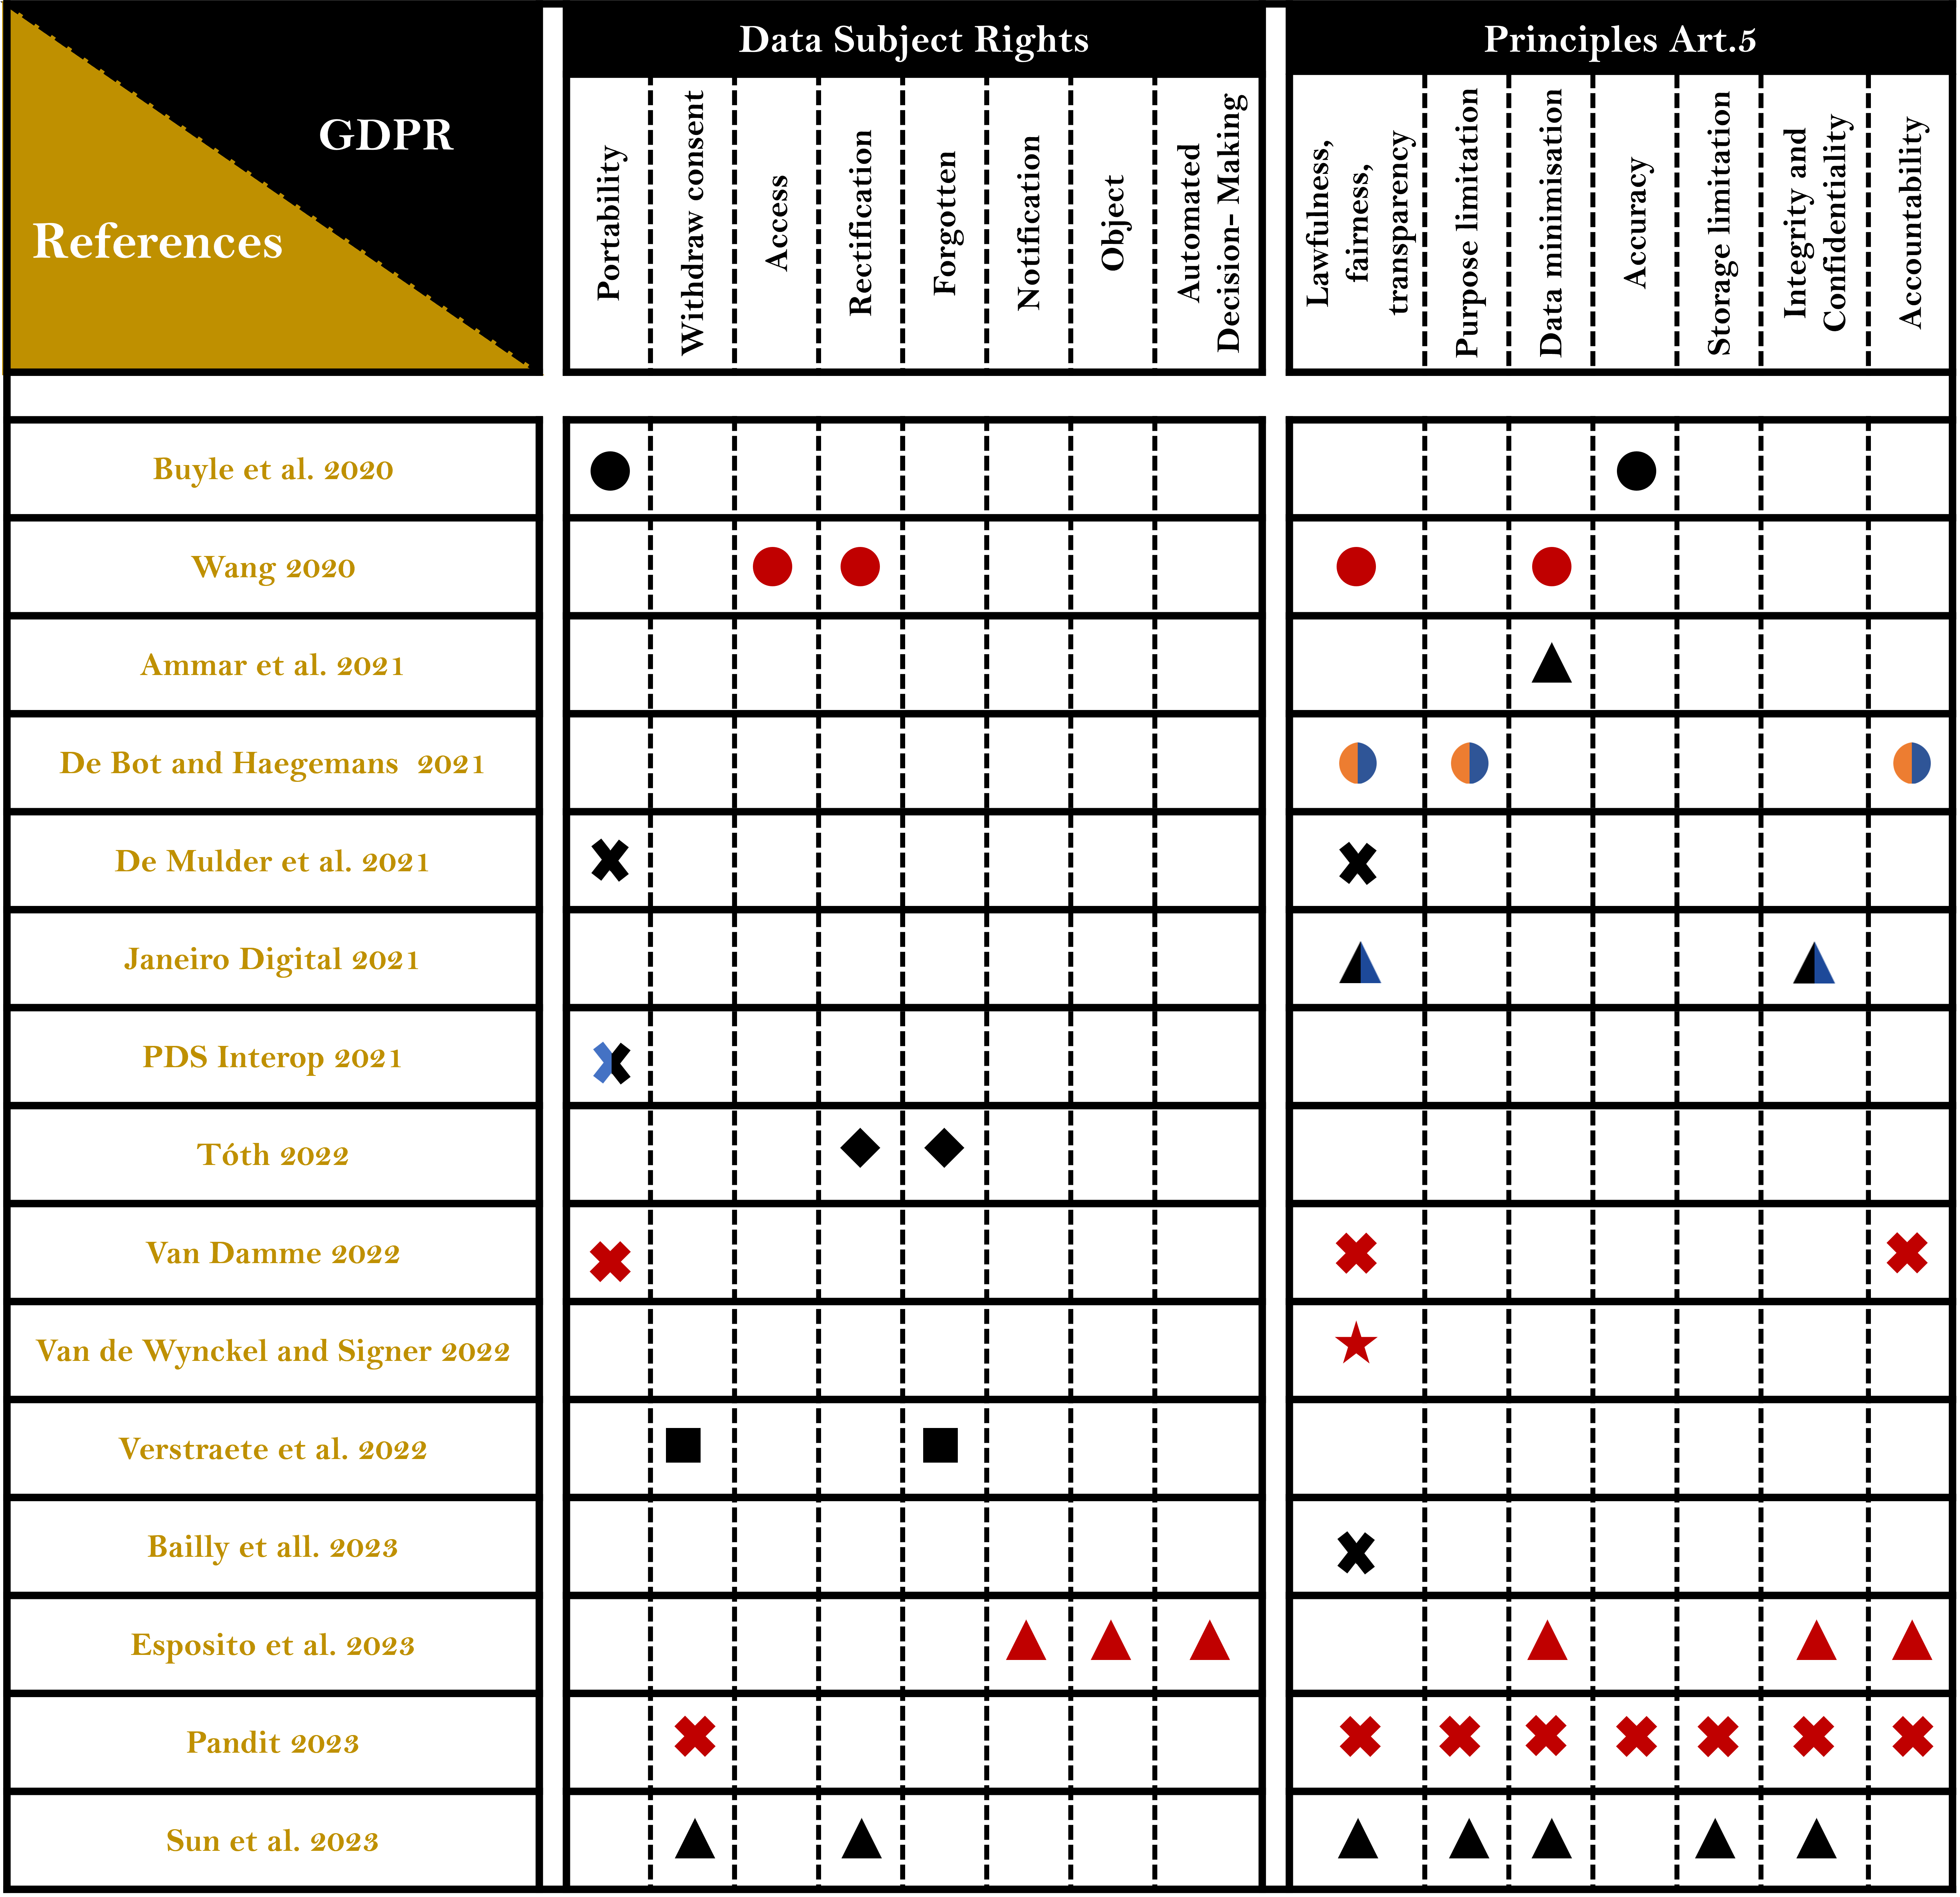
\includegraphics[width=\textwidth]{figures/chapter-2/solid-sota.png}
\caption[Comparison of existing work on Solid and data protection topics.]{Comparison of existing work on Solid and data protection topics. Each work was analysed in terms of whether it assists in the exercising of data subject rights or in the implementation of a certain GDPR principle, as well as the type of solution they developed -- works describing Solid apps are marked with a \textbf{black} shape, identity provider solutions with a \textbf{\textcolor{orange}{orange}} shape, Pod provider solutions with a \textbf{\textcolor{blue}{blue}} shape and theoretical work with a \textbf{\textcolor{red}{red}} shape. In addition, works marked with a $\medcircle$ discuss a government-related use case, $\medtriangleup$ a health-related use case, $\meddiamond$ a hospitality-related use case, \faStarO\space a location-related use case, $\medsquare$ a human resources-related use case and \textbf{X} represents work without a particular domain-related use case.}
\label{fig:solid_sota}
\end{figure}

As illustrated by the Figure, most works concentrate on fulfilling one or more GDPR principles, with a strong focus on the \textit{`lawfulness, fairness and transparency'} principle.
Distinct works were also found to tackle the right to data portability, withdrawal of consent, and rectification, while no specific work was found on the right to restrict the processing of personal data.

\subsection{Other decentralised technologies}
\label{sec:sota_other_technologies}

In addition to Solid and its stack of technologies, there is a set of tools and resources that support decentralisation and are either being discussed or should be discussed to be included in the Solid ecosystem.
We briefly present them in this Section as they should be considered in future research in this area.

\paragraph{Decentralised Identity}
The Decentralized identifiers (DIDs) data model is a recent W3C Recommendation that enables \textit{``individuals and organizations to generate their own identifiers using systems they trust''}~\citep{sporny_decentralized_2022}\footnote{A DID Solid method specification is in the early stages of development, with no official implementations being known to date -- available at \url{https://solid.github.io/did-method-solid/} (accessed on 19 August 2023).}.
In contrast with centralised settings, DIDs allow something or someone to be identified by a globally unique identifier which is detached from centralised registries, identity providers, or certificate authorities.
Moreover, DIDs work in a similar fashion to WebIDs -- DIDs are still URIs that can be dereferenced to return a DID document which \textit{``can express cryptographic material, verification methods, or services [...] to prove control of the DID''}.
The European Commission is also promoting the emergence of digital identity wallets for EU citizens, residents, and businesses to identify themselves, both online and offline, and to exchange certain types of personal identification data such as birth certificates or driving licenses.
In this context, the electronic IDentification, Authentication and trust Services (eIDAS) regulation~\citeyearpar{noauthor_regulation_2014}, and its amendment~\citeyearpar{noauthor_eidas2_2021}, puts forward \textit{``rules for trust services''} and \textit{``a legal framework for electronic signatures, electronic seals, electronic time stamps, electronic documents, electronic registered delivery services and certificate services for website authentication''}, while the 2021 amendment explicitly adds \textit{``conditions for the issuing of European Digital Identity Wallets''} and additional considerations derived from the GDPR.

\paragraph{Verifiable Credentials}
W3C's Verifiable Credentials (VCs) data model specification describes \textit{``a standard way to express credentials on the Web in a way that is cryptographically secure, privacy-respecting, and machine-verifiable''}~\citep{sporny_verifiable_2023}, using technologies such as digital signatures.
As in the physical world, VCs can be used to identify data subjects, to provide government-issued documents, e.g., ID cards or passports, or to deliver information on how the credential was created/derived and other constraints such as validity period or conditions for use.
An example of a VC, with a DID-identifiable subject, is presented in Listing \ref{list:vc_fromspec}.
The usage of VCs is being contemplated in the ACP specification, however, no specific details are provided regarding its implementation/development.

\begin{listing}[ht]
\caption[Verifiable credential with terms of use.]{Verifiable credential with terms of use where the issuer is prohibiting verifiers from archiving a degree credential, extracted from~\cite{sporny_verifiable_2023}, with the credential subject being identified by a DID.}
\label{list:vc_fromspec}
\begin{minted}{json}
{
    "@context": [
        "https://www.w3.org/ns/credentials/v2",
        "https://www.w3.org/ns/credentials/examples/v2"
    ],
    "id": "http://university.example/credentials/3732",
    "type": ["VerifiableCredential", "ExampleDegreeCredential"],
    "issuer": "https://university.example/issuers/14",
    "validFrom": "2010-01-01T19:23:24Z",
    "credentialSubject": {
        "id": "did:example:ebfeb1f712ebc6f1c276e12ec21",
        "degree": {
          "type": "ExampleBachelorDegree",
          "name": "Bachelor of Science and Arts"
        }
    },
    "termsOfUse": [{
        "type": "IssuerPolicy",
        "id": "http://example.com/policies/credential/4",
        "profile": "http://example.com/profiles/credential",
        "prohibition": [{
            "assigner": "https://university.example/issuers/14",
            "assignee": "AllVerifiers",
            "target": "http://university.example/credentials/3732",
            "action": ["Archival"]
        }]
    }] 
}
\end{minted}
\end{listing}

Moreover, \cite{braun_selfverifying_2022,braun_attributebased_2022} have previously published work on using VCs and RDF-star\footnote{RDF-star\citep{arndt_rdfstar_2023} is an under-development W3C specification that \textit{``extends RDF with a convenient way to make statements about other statements''}.} to sign and verify Web resources using a Solid app\footnote{The source code is available at \url{https://github.com/uvdsl/solid-web-ldsig}, under an MIT license (accessed on 19 August 2023).} and on using VCs and Linked Data Notifications (LDNs)\footnote{The W3C LDNs Recommendation \citep{capadisli_linked_2017} is a protocol that describes how servers can send and retrieve RDF-based messages, sent/retrieved by applications.}, extending previous work from~\citeauthor{ezike_solidvc_2019}, to request attribute-based access to Solid Pods\footnote{The source code is available at \url{https://github.com/uvdsl/solid-vc-pwa/}, under an MIT license (accessed on 19 August 2023).}.
\section{Representing personal data processing information}
\label{sec:sota_vocabularies}

The Web of Data and its semantic specifications are thriving, with the W3C guiding this effort to have machine-readable and interoperable linked data on the Web, described by open standards which promote portability and extensibility, allow for seamless integration of data from different origins and re-usage across distinct Web applications and services \citep{berners-lee_semantic_2001}.
Accordingly, a wave of vocabularies and ontologies has appeared in the last few years to formalise common concepts, such as objects or entities, or terms from specific domains, such as legal or medical ontologies.
More recently, with the increasing concerns around personal data processing abuse by Big Tech companies, data protection has been on the agenda of governments in a worldwide manner, with the EU taking the lead with its data protection law, the GDPR.
This has led to a new wave of personal data protection law ontologies being developed to help companies to comply with GDPR's legal requirements and which also intend to assist individuals to manage their personal data.

In the following Sections, the criteria used to analyse each specified data protection vocabulary are included, as well as a description of each identified solution.

\subsection{Criteria for analysis}
\label{sec:sota_vocabularies_criteria}

For each identified solution, we describe the core terms formalised in the ontologies, as well as dependencies on other existing works, and, when available, case studies where it has been applied.
As for the analysis of their representational abilities, we analyse whether such ontologies can represent the privacy terms mentioned in GDPR's data subject rights, to assess to what extent they can be used by data subjects to exercise their rights and by data controllers to manage compliance.

In particular, the so-called \textit{`right to be informed'}, described in detail on Articles 13 and 14, obliges data controllers to inform data subjects about any processing of personal data, whether being from data collected directly from the data subjects or from other sources. In addition to this, the following rights are also provided to data subjects:

\begin{enumerate}
  \item[(Art. 15)] \textit{`right of access'} to the personal data being processed, including a copy of the data as well as information about the purposes for processing, categories of the personal data being processed and their source, any recipients to whom the data may have been shared and corresponding measures to ensure its security, storage and retention conditions and the existence of other data subject's rights.
  \item[(Art. 16)] \textit{`right to rectification'} of inaccurate or incomplete personal data.
  \item[(Art. 17)] \textit{`right to be forgotten'}  by the data controllers when the personal data is no longer needed for the purposes for which it was collected.
  \item[(Art. 18)] \textit{`right to restriction of processing'} of personal data when its accuracy is being contested, the processing is unlawful, when the data subject needs it for any legal claims or objects to the processing.
  \item[(Art. 19)] \textit{`right to be notified'} about the rectification, erasure or restriction of processing.
  \item[(Art. 20)] \textit{`right to data portability'}, including the right to request that said data be transferred directly from one controller to another.
  \item[(Art. 21)] \textit{`right to object'} to any processing, including profiling.
  \item[(Art. 22)] \textit{`right to not be subjected to automated decision-making'}, including profiling.
\end{enumerate}

For such rights to be exercised by data subjects and fulfilled by data controllers, a set of privacy terms must be modelled, namely the terms identified in Table \ref{tab:GDPR_privacy_terms}, which is derived from \cite{esteves_analysis_2022}. These terms will be used to compare the described privacy and data protection vocabularies and ontologies and identify representational gaps in the existing solutions. The outcomes of this comparative analysis will be provided in Section \ref{sec:sota_vocabularies_analysis}.

\begin{table}
\centering
\caption{Privacy terms to be represented and respective identifiers (I*). The GDPR articles that mention these terms are also specified.}
\label{tab:GDPR_privacy_terms}
\resizebox{\textwidth}{!}{%
\begin{tabular}{c||l|c}
 I* & Informational Items & \textbf{GDPR Article(s)} \\
 \hline\hline
 I1 & Controller identity & \textbf{13.1(a), 14.1(a)} \\
 \hline
 I2 & Controller contact details & \textbf{13.1(a), 14.1(a)} \\
 \hline
 I3 & Controller's representative identity & \textbf{13.1(a), 14.1(a)} \\
 \hline
 I4 & Controller's representative contact details & \textbf{13.1(a), 14.1(a)} \\ 
 \hline
 I5 & DPO contact details & \textbf{13.1(b), 14.1(b)} \\
 \hline
 I6 & Purposes of the processing & \textbf{13.1(c), 14.1(c), 15.1(a)} \\ 
 \hline
 I7 & Legal basis of the processing & \textbf{6.1, 9.2, 13.1(c), 14.1(c)} \\ 
 \hline
 I8 & Legitimate interests & \textbf{6.1(f), 13.1(d), 14.2(b)} \\ 
 \hline
 I9 & Recipients / categories of recipients & \textbf{13.1(e), 14.1(e), 15.1(c), 17.2, 19} \\
 \hline
 I10 & Transfers to third countries & \textbf{13.1(f), 14.1(f)} \\ 
 \hline
 I11 & Retention period & \textbf{13.2(a), 14.2(a), 15.1(d)} \\ 
 \hline
 I12 & Data subject's rights & \textbf{13.2(b), 14.2(c), 15.1(e)} \\ 
 \hline
 I13 & Right to withdraw consent & \textbf{6.1(a), 9.2(a), 13.2(c), 14.2(d)} \\ 
 \hline
 I14 & Right to lodge a complaint & \textbf{13.2(d), 14.2(e), 15.1(f)} \\ 
 \hline
 I15 & Statutory or contractual obligation details & \textbf{13.2(e)} \\ 
 \hline
 I16 & Existence of automated decision making & \textbf{13.2(f), 14.2(g), 15.1(h), 22.1, 22.4} \\ 
 \hline
 I17 & Categories of personal data & \textbf{9.1, 14.1(d), 15.1(b)} \\ 
 \hline
 I18 & Source of personal data & \textbf{14.2(f), 15.1(g)} \\ 
 \hline
 I19 & Grounds to not comply with information right & \textbf{13.4, 14.5} \\
 \hline
 I20 & Safeguards related to the transfer to a third country & \textbf{15.2} \\ 
 \hline
 I21 & Copy of personal data & \textbf{15.3, 20.1} \\ 
 \hline
 I22 & Request to complete incomplete personal data & \textbf{16} \\ 
 \hline
 I23 & Grounds to request erasure of data & \textbf{17.1} \\ 
 \hline
 I24 &  Technical measures taken to erase data & \textbf{17.2} \\
 \hline
 I25 & Recipients contact details & \textbf{17.2, 19} \\
 \hline
 I26 & Grounds to not comply with right of erasure & \textbf{17.3} \\
 \hline
 I27 & Grounds to request restriction of processing & \textbf{18.1} \\
 \hline
 I28 & Transfer data directly between controllers & \textbf{20.2} \\
 \hline
 I29 & Grounds to not comply with right to object & \textbf{21} \\
 \hline
 I30 & \multicolumn{1}{l|}{\begin{tabular}[l]{@{}l@{}} Grounds to not comply with right not to be \\ subjected to decision making \end{tabular}} & \textbf{22.2} \\
\end{tabular}}
\end{table}

\subsection{Personal data protection vocabularies}
\label{sec:sota_vocabularies_description}

% TODO: https://openscience.adaptcentre.ie/ontologies/GConsent/docs/ontology#related-work 

In this Section, a systematic description of each identified work is provided, including an example that uses the vocabulary's concepts, when available.
Moreover, Table \ref{tab:analysed_vocabularies} provides an overview of these solutions and supplies information about the creators of the resources, their versions, the date of publication and the date of the last known update.
Said solutions are then analysed in chronological order regarding the date of publication and a dependency graph -- a chart that demonstrates the relations between the reviewed vocabularies and its dependencies and extensions -- is presented in Figure \ref{fig:voc_dependency_graph}.

\begin{table}
\centering
\caption{Brief description of the vocabularies described in Section \ref{sec:sota_vocabularies_description}.}
\label{tab:analysed_vocabularies}
\resizebox{\textwidth}{!}{%
\begin{tabular}{c||c|c|c|c|c}
Abbreviation (Section) & Full Name & Creators & Version & \multicolumn{1}{c|}{\begin{tabular}[c]{@{}c@{}} Date of \\ publication \end{tabular}} & \multicolumn{1}{c}{\begin{tabular}[c]{@{}c@{}} Last \\ update \end{tabular}} \\
 \hline\hline
 \multicolumn{1}{c||}{\begin{tabular}[c]{@{}c@{}} DPKO, \\ DPRO (\ref{sec:neurona}) \end{tabular}} & \multicolumn{1}{c|}{\begin{tabular}[c]{@{}c@{}} Data Protection Knowledge Ontology, \\ Data Protection Reasoning Ontology \end{tabular}} & Casellas et al. & - & 2008 & 2010 \\
 \hline
 DPO (\ref{sec:dpo}) & Data Protection Ontology & Bartolini and Muthuri & - & 2015 & 2016 \\
 \hline
 GDPRov (\ref{sec:gdprov}) & GDPR Provenance Ontology & Pandit and Lewis & 0.7 & 2017 & 2019 \\
 \hline
 Cloud (\ref{sec:cloud}) & Cloud GDPR ontology & Elluri and Joshi & - & 2018 & - \\
 \hline
 PrOnto (\ref{sec:pronto}) & Privacy Ontology for legal reasoning & Palmirani et al. & - & 2018 & - \\
 \hline
 GConsent (\ref{sec:gconsent}) & GDPR Consent ontology & Pandit et al. & 0.5 & 2018 & - \\
 \hline
 IMO (\ref{sec:imo}) & Information Model Ontology & Lioudakis and Cascone & 1.0 & 2018 & - \\
 \hline
 DPV (\ref{sec:dpv}) & Data Privacy Vocabulary & Pandit et al. & 1.0 & 2018 & 2022 \\
 \hline
 \hline
 GDPRtEXT (\ref{sec:gdprtext}) & GDPR text EXTensions & Pandit et al. & 0.7 & 2018 & 2020 \\
\end{tabular}}
\end{table}

\begin{figure}
\caption{Data protection vocabularies dependency chart.}
\label{fig:voc_dependency_graph}
\centering
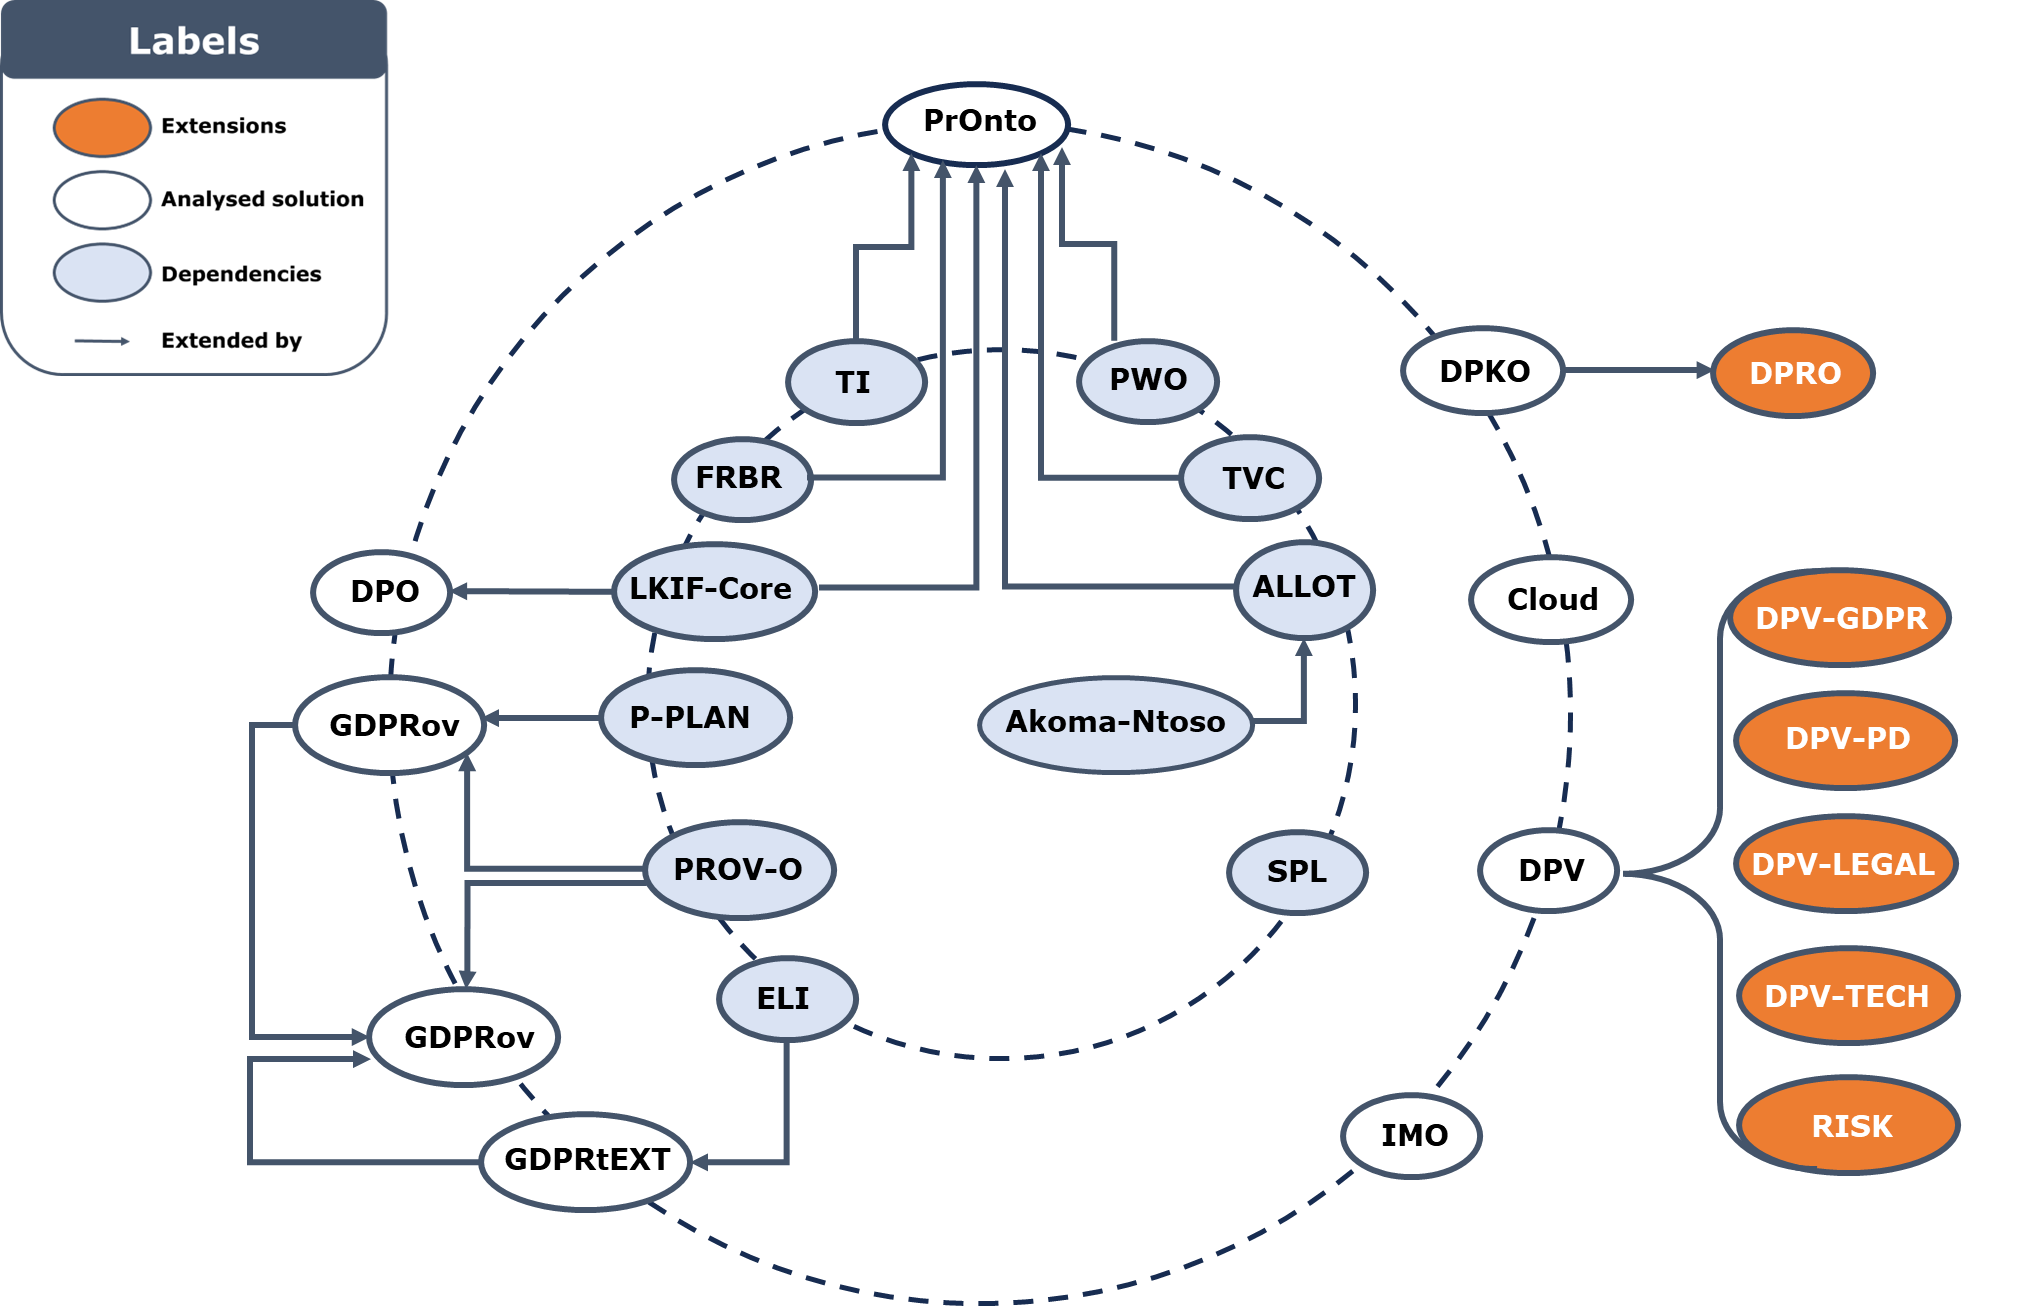
\includegraphics[width=\textwidth]{figures/chapter-2/vocabs.png}
\end{figure}

To complement the description of vocabularies presented in this Section, additional documentation and resources were published in a Web page\footnote{Available at \url{https://protect.oeg.fi.upm.es/sota/ontologies}. Its public repository can be consulted at \url{https://github.com/besteves4/SotAResources} for further improvement when new solutions appear.}, including diagrams and code examples.

\subsubsection{NEURONA}
\label{sec:neurona}

The NEURONA project \citep{casellas_ontological_2010}, developed by S21SEC\footnote{\url{https://www.s21sec.com/} (accessed on 16 July 2023)} and IDT-UAB\footnote{\url{https://portalrecerca.uab.cat/en/organisations/law-and-technology-institute} (accessed on 16 July 2023)}, created two ontologies based on the pre-GDPR Spanish personal data protection regulation \citeyearpar{noauthor_real_2008} -- the Data Protection Knowledge Ontology (DPKO) and the Data Protection Reasoning Ontology (DPRO).
These ontologies are, however, not publicly available for re-usage.

The main objectives of the ontologies developed in the context of this project were to represent security measures for files containing personal data and reason over their correctness.
DPKO's main classes are \textbf{data}, \textbf{consent}, \textbf{purpose}, \textbf{person}, \textbf{security measures} and \textbf{security degree}.
In relation to the data class, categories such as health data are defined and associated with special security measures. 
The consent should be given by the data subject in an unambiguous way and for a specific purpose.
In addition, technical and organisational measures (TOMs) for data security, such as access control measures or authentication procedures, are modeled and connected to the nature of the data, taking into consideration the security level associated with the type of data or how the data was obtained. 
For example, a file with health data obtained without consent should have high-level security measures, while a file with anonymised data can implement low-level measures.
DPRO is then used to access data protection compliance by reasoning over the measures applied to files.

\subsubsection{DPO}
\label{sec:dpo}

The Data Protection Ontology (DPO) \citep{bartolini_reconciling_2015,otake_using_2017} concentrates on the modelling of data protection principles and data controller obligations. It is based on an early version of the GDPR, prior to its implementation in May 2018, on the Data Protection Directive \citeyearpar{noauthor_directive_1995} and the \textit{Handbook on European data protection law} \citep{european_union_agency_for_fundamental_rights_and_council_of_europe_handbook_2018} and reuses concepts from the LKIF-Core \citep{hoekstra_lkif_2007} ontology.

The core classes of DPO are \textbf{data protection principles}, \textbf{rules} for processing and transferring data, and \textbf{data subjects rights}.
The ontology is designed so that each rule and right is linked to at least one principle.
For instance, data subjects have the right to rectify inaccurate or incomplete data and data controllers must provide the means to do it, according to GDPR's \textit{`accuracy'} principle.
Furthermore, DPO defines consent as a legal justification connected with the principle of trust and also specifies concepts to model the special case of giving consent as a parent for a child, although the concept of \textit{`consent provided by delegation'} is missing.
Data protection-related entities, such as data controllers, supervisory authorities, processors, representatives or data protection officers, are modelled as a type of \textbf{person}.

Listing \ref{list:sparql_dpo} provides an example of a SPARQL query to retrieve duties of a data controller that do not concern the transfer of personal data using DPO.\footnote{More examples are available in a project repository at \url{https://bitbucket.org/guerret/lu.uni.eclipse.bpmn2/} (accessed on 16/July/2023).}

\begin{listing}
\caption{SPARQL query to retrieve duties of the data controller that do not concern data transfer using the Data Protection Ontology.}
\label{list:sparql_dpo}
\begin{minted}{sparql}
SELECT DISTINCT ?duty WHERE {
    ?x rdfs:subClassOf* [ rdf:type dpo:Rule ] .
	?x rdfs:label ?duty
	MINUS {
		?x rdfs:subClassOf* [ rdf:type dpo:TransferRule ] .
		?x rdfs:label ?duty .
	} .
	FILTER (?duty != "Rule"@en && ?duty != "ProcessingRule"@en && ?duty != "TransferRule"@en) }
\end{minted}
\end{listing}

\subsubsection{GDPRov}
\label{sec:gdprov}

The GDPR Provenance Ontology (GDPRov) \citep{pandit_modelling_2017} aims to record the provenance of personal data and of the consent conditions and processing activities performed over such data, according to the GDPR.
GDPRov extends PROV-O \citep{lebo_prov-o_2013}, a W3C Recommendation created to define the provenance of entities and systems, and P-Plan \citep{garijo_augmenting_2012}, an extension of PROV-O to represent activities and corresponding steps to execute them, as well as the entities involved.
Using these terms, it is possible to monitor changes in consent or to track the interaction between entities involved in the exchange of data.

GDPRov's main concept to record the provenance of consent is the \textbf{consent agreement template} class, a common template which includes the consent conditions presented to the users and the entities in charge of data  processing, and also information on third party sharing, approved processing activities and additional rights.
Provenance metadata on the origin, use, storage and sharing of the data can also be recorded with GDPRov, as well as information regarding transformations performed to the data.
In addition to this, provenance data on the exercising and fulfilment of GDPR-related rights and obligations can also be represented with GDPRov -- for each right or obligation, a plan can be modelled to include the activities that need to be executed when an user exercises a particular right.

Listing \ref{list:sparql_gdprov} illustrates a SPARQL query which uses GDPRov's terms to retrieve the entities involved in acquiring consent.

\begin{listing}
\caption{SPARQL query retrieving entities involved in acquiring consent using GDPRov \citep{pandit_modelling_2017}.}
\label{list:sparql_gdprov}
\begin{minted}{sparql}
SELECT ?consent ?template ?toc WHERE {
    ?consent a gdprov:ConsentAgreement .
    ?template a gdprov:ConsentAgreementTemplate .
    ?toc a gdprov:TermsAndConditions .
    ?step a gdprov:ConsentAcquisitionStep .
    ?step gdprov:usesConsentAgreementTemplate ?template .
    ?step gdprov:usesTermsAndConditions ?toc .
    ?step gdprov:generatesConsentAgreement ?consent }
\end{minted}
\end{listing}

\subsubsection{Cloud}
\label{sec:cloud}

The Cloud GDPR ontology was developed by \cite{elluri_knowledge_2018} to express data protection obligations of cloud data consumers and providers, taking into consideration the Cloud Security Alliance (CSA) controls defined on the \textit{Code of Conduct for GDPR Compliance} \citep{cloud_security_alliance_-_privacy_level_agreement_working_group_code_2017}.

The \textbf{stakeholders}, \textbf{controls} and \textbf{obligations} are the core concepts of this ontology.
Cloud-related obligations are extracted and connected to GDPR's articles and are also associated to CSA requirements using the \textbf{hasCSAcontrol} property.
Moreover, these obligations are further specified into common or provider/consumer-specific obligations taking into consideration which stakeholders they are applicable to, e.g., maintaining records of data processing activities and notifying data breaches are common obligations, while providing legal representatives for non-EU stakeholders or hiring a DPO are the responsibility of the consumer and of the provider, respectively.

This work was later extended \citep{elluri_integrated_2018} to automate the implementation of compliance tasks mandated by the GDPR and the Payment Card Industry Data Security Standard (PCI DSS) guidelines \citep{pci_security_standards_council_payment_2018} and also to include the rights of consumers, providers and end users.
These guidelines deal with financial data, such as the credit card number or card-holder's name, which fall under the protection offered by the GDPR.
As such, and since its scope is narrower, a data breach of PCI DSS-related data automatically results in GDPR-related one.
Thus, the cloud-related PCI DSS requirements were used to enhance this ontology and its evaluation was performed using privacy policies from five major companies that deal with card-holder's data.

\subsubsection{PrOnto}
\label{sec:pronto}

PrOnto, the Privacy Ontology for legal reasoning, aims to model GDPR-related associations between agents, processing activities, data categories and deontic modalities, with the main goal to support legal reasoning and compliance with data protection regulations \citep{ko_pronto_2018}.
PrOnto relies on a number of ontologies to model these relationships:
\begin{itemize}
    \item LKIF-Core \citep{hoekstra_lkif_2007} is used to model agents, e.g., organisations, software or people, as well as the several legal roles which can be assigned to them, i.e., acting as a data controller or processor.
    \item The Functional Requirements for Bibliographic Records (FRBR) ontology \citep{byrum_functional_2009} is used to model legal documents as sources of information, that regulate the different relationships between the agents documented in the text, and to register changes in their representation over time. % copied
    \item The ALLOT (A Light Legal Ontology On Top level classes) ontology, developed by Barabucci et al. \citep{barabucci_managing_2010}, extends the Akoma Ntoso standard \citep{palmirani_akoma-ntoso_2011} to link documents with the data they contain, e.g., people, events or locations.
    \item The Publishing Workflow Ontology (PWO) \citep{gangemi_publishing_2017} is used to characterize provenance data associated with the publication of a document, e.g., to model the different types of processing of personal data.
    \item The TVC (Time-indexed Value in Context) ontology \citep{peroni_semantic_2014} and the TI (Time Interval) ontology pattern\footnote{\url{http://www.ontologydesignpatterns.org/cp/owl/timeinterval.owl} (accessed on 16/July/2023)} are used to associate time-dependant variables such as events to specific agent roles that only emerge in particular point in time.
\end{itemize}

PrOnto's main classes are defined as follows: \textbf{documents and data}, \textbf{agents and roles}, \textbf{processing and workflow}, \textbf{legal rules and deontic formula}, and \textbf{purposes and legal bases}.
GDPR is the main document used to extract personal data categories such as judicial or sensitive data and non-personal data such as anonymous or legal person data.
Moreover, processing activities are represented as a workflow of actions that should be recorded together with provenance data such as the context and time in which each action occurs.
Each processing activity is also associated with a purpose and a legal rule, which is composed of deontic specifications, i.e., prohibitions, rights, permissions and obligations, used to check if the activity being executed is compliant with the GDPR. PrOnto is, however, not publicly available for re-usage, which hinders the assessment of the totality of concepts it models\footnote{As PrOnto is not available online, its namespace is unknown. We use the prefix \texttt{pronto} to identify PrOnto's concepts that are available in the analysed publication.}. 

Listing \ref{list:sparql_pronto} illustrates a query to retrieve information regarding personal data processing activities performed by company X in the role of controller from time t1 to t2.

\begin{listing}
\caption{SPARQL query used to retrieve personal data processing activities performed by company X in the role of controller from t1 to t2 using PrOnto \citep{ko_pronto_2018}.}
\label{list:sparql_pronto}
\begin{minted}{sparql}
SELECT ?pdp WHERE {
    ?pdp pronto:isManagedBy _:c .
    [ lkif:plays _:c ;
        rdfs:label "X" ] .
    ?pdp pronto:isValid [
        ti:hasIntervalStartDate [ 
            a ti:TimeInterval; rdfs:label "t1" ] ;
        ti:hasIntervalEndDate [ 
            a ti:TimeInterval; rdfs:label "t2" ] ] . }
\end{minted}
\end{listing}

\subsubsection{GConsent}
\label{sec:gconsent}

GConsent \citep{hitzler_gconsent_2019} is an ontology focused on the GDPR concept of consent and, as such, it models information regarding how consent was collected and stored, as well as records of any changes that may occur over time, including withdrawal, including data on the parties involved, according to Article 6 of the GDPR.
Additionally, other documentation sources were also adopted, including EDPB's guidelines on consent \citep{european_data_protection_board_guidelines_2020}.
As GConsent aims at not only capturing the concept of consent, but also to represent its state, context and provenance, existing vocabularies on this subject, such as PROV-O \citep{lebo_prov-o_2013}, GDPRov \citep{pandit_modelling_2017} and GDPRtEXT \citep{gangemi_gdprtext_2018} -- later presented in Section \ref{sec:gdprtext}, are reused. % copied

GConsent's main concepts are the terms to represent \textbf{data subjects}, \textbf{personal data}, \textbf{purpose} and \textbf{processing types}, as well as the \textbf{consent} and \textbf{consent status} classes -- the latter fills a gap on the available ontologies on this domain as it not only defines \textbf{explicitly given consent} as a concept, but also classifies other states of consent, such as \textbf{implicitly given}, \textbf{expired} or \textbf{refused}.
GConsent also includes concepts to represent information regarding the context in which the consent was obtained -- information about the entities involved, spatial and temporal aspects and the format used to record it, e.g., Web form, voice recording or signature -- and a taxonomy of processing types, e.g., data alignment or data retrieval.

Listing \ref{list:ttl_gconsent} provides an example of a record of provenance data regarding an activity of withdrawing consent using GConsent.

\begin{listing}
\caption{Turtle record of provenance data regarding an activity of withdrawing consent using GConsent \citep{hitzler_gconsent_2019}.}
\label{list:ttl_gconsent}
\begin{minted}{turtle}
_:modifyConsent a gdprov:ModifyConsentActivity ;
    prov:invalidated _:consent1 ;
    prov:generated _:consent2 .

_:consent1 a gc:Consent ;
    gc:isPreviousConsentFor _:consent2 ;
    gc:hasStatus gc:ConsentStatusExplicitlyGiven .

_:consent2 a gc:Consent ;
    gc:hasStatus gc:ConsentStatusWithdrawn .
\end{minted}
\end{listing}

\subsubsection{IMO}
\label{sec:imo}

The Information Model Ontology (IMO) \citep{papagiannakopoulou_leveraging_2014,lioudakis_compliance_2019} was developed in the context of the BPR4GDPR project\footnote{BPR4GDPR (Business Process Re-engineering and functional toolkit for GDPR compliance) is an European Union H2020 innovation programme with the main goal of providing a framework to reinforce the implementation of GDPR-compliant measures inside organizations at diverse scales and in several domains. More information available at \url{https://www.bpr4gdpr.eu/} (accessed on 16/July/2023).} and it aims to define the entities and respective roles that are involved in the organisation lifecycle of processing personal data.

IMO's core classes are \textbf{data types}, \textbf{roles} assigned to users within different \textbf{organization types}, \textbf{machine types} that host \textbf{operations} for particular \textbf{purposes}, \textbf{events} and their \textbf{context} information.
The roles class is related to the responsibilities that are assigned to the user in the context of the organization and its instances can be implemented hierarchically according to the detail level of the data and connected through the \textit{isA} property -- a structure which is valid for most classes in the ontology. % copied
The data processing activities are implemented through the operations class, which have associated the \textit{hasInput} and \textit{hasOutput} properties that allow to connect the operations with the data that is processed and the one that is generated and respective states, i.e., plain or anonymised. % copied
These operations can be grouped in an operation container -- a class that groups processing activities in contexts where they usually work together, for instance, in the management of a database, in which functions such as create, read, update or delete are commonly used.  % copied
The roles and operations classes should always be connected with an instance of the purpose class.  % copied
The events class, that aims at capturing all processing activities, a data breach or the revoke of consent, has associated the context class to instantiate specific cases and provide temporal and spatial details, among others.  % copied

% TODO: extract example from https://www.researchgate.net/profile/Joaquin-Garcia-Alfaro/publication/260706010/figure/fig3/AS:296857856167938@1447787836426/Example-of-Ontological-Access-Control-Rule.png

\subsubsection{DPV}
\label{sec:dpv}

The Data Privacy Vocabulary is being developed and maintained by the W3C Data Protection Vocabularies and Controls Community Group (DPVCG)\footnote{\url{https://www.w3.org/community/dpvcg/} (accessed on 16/July/2023)} -- an output of a W3C workshop on data privacy controls which took place in 2018, with the objective of defining priorities for the standardization of this domain \citep{bonatti_data_2018}.

DPV's core concepts, \textbf{processing}, \textbf{purpose}, \textbf{recipient} and \textbf{personal data categories}, were adapted from the SPECIAL Usage Policy Language (SPL) vocabularies \citep{bonatti_policy_2018} and new concepts were/are continuously added to DPV after being discussed and agreed upon by the Community Group.
In addition to previously mentioned concepts, DPV's base vocabulary was first published with the following additional classes: \textbf{legal basis}, \textbf{technical and organizational measures} and \textbf{legal entities}, including \textbf{data subject} and \textbf{child}, \textbf{recipients}, \textbf{data controller}, \textbf{data processor} and \textbf{third party} \citep{panetto_creating_2019}.
In December of 2022, DPV version 1 was published including additional concepts to model \textbf{risk}, \textbf{rights} and \textbf{data subject rights}, \textbf{technology}, \textbf{laws} and \textbf{context of processing} classes and the previously existing taxonomies were extended with new terms -- new legal entities, including authority and data protection authority, vulnerable data subject, data sub-processor, data protection officer and representative, were added to the vocabulary, as well as new purpose and legal basis sub-classes.
For instance, the purpose taxonomy is composed of 76 purpose sub-classes, which are topped by classes such as R\&D or Service Provision, and can be further constrained to specific contexts or business sectors, and DPV's processing operations taxonomy covers the terms defined in Article 4.2 of the GDPR, providing a set of 44 processing categories.

DPV also provides five extensions:
\begin{itemize}
    \item Personal data categories are defined in the DPV-PD extension\footnote{\url{https://w3id.org/dpv/dpv-pd} (accessed on 17/July/2023)} -- the personal data class is split into generic classes such as financial or social data, adapted from the \textbf{EnterPrivacy} taxonomy by \cite{cronk_categories_2017}, which are further specified into concepts such as credit card number or social media accounts.
    \item GDPR-specific concepts are defined in the DPV-GDPR extension\footnote{\url{https://w3id.org/dpv/dpv-gdpr} (accessed on 17/July/2023)} -- it covers legal bases specified on GDPR's Articles 6 and 9 for the processing of personal data and also the legal bases for the transfer of personal data to third countries defined on Articles 45, 46 and 49. It also models GDPR's data subject rights, data transfer tools and Data Protection Impact Assessment (DPIA) terms.
    \item Technology-relevant concepts are defined in the DPV-TECH extension\footnote{\url{https://w3id.org/dpv/dpv-tech} (accessed on 17/July/2023)} -- it includes concepts to model specific technologies, their management, technology actors and relevant tools and systems.
    \item Jurisdiction-relevant concepts are defined in the DPV-LEGAL extension\footnote{\url{https://w3id.org/dpv/dpv-legal} (accessed on 17/July/2023)} -- it contains terms related to specific laws, adequacy decisions and a taxonomy of authorities.
    \item Risk concepts are defined in the RISK extension\footnote{\url{https://w3id.org/dpv/risk} (accessed on 17/July/2023)} -- it covers concepts related to risk, likelihood, severity levels, consequences and impacts, as well as risk assessment techniques and methodologies.
\end{itemize}

Listing \ref{list:ttl_dpv} provides an example of a personal data handling related to the collection and usage of email addresses for marketing purposes using DPV.

\begin{listing}
\caption{Turtle record of a personal data handling related to the collection and usage of email addresses for marketing purposes using DPV \citep{panetto_creating_2019}.}
\label{list:ttl_dpv}
\begin{minted}{turtle}
_:AcmeMarketing a dpv:PersonalDataHandling ;
    dpv:hasDataController [ a dpv:DataController ] ;
    dpv:hasPersonalData dpv-pd:EmailAddress ;
    dpv:hasProcessing dpv:Collect, dpv:Use ;
    dpv:hasPurpose dpv:Marketing .
\end{minted}
\end{listing}

\subsubsection{GDPRtEXT}
\label{sec:gdprtext}

GDPRtEXT was developed by \cite{gangemi_gdprtext_2018} as a linked data resource, which extends the European Legislation Identifier (ELI) ontology \citep{office_of_publications_on_eur-lex_eu_2017}, to connect GDPR concepts with the specific chapters, articles or points of the regulatory text.

The main concepts modelled in this ontology are related to the specific \textbf{entities} mentioned in the GDPR text, their \textbf{rights} and \textbf{obligations}, the \textbf{principles} and the \textbf{activities} which specify processes and actions defined in the GDPR, such as reporting a data breach, exercising rights or demonstrating consent.
These terms are linked to the relevant GDPR articles using the \textbf{rdfs:isDefinedBy} property.

\subsection{Comparative analysis}
\label{sec:sota_vocabularies_analysis}

% TODO: \beatriz{DPKO: I7 - only consent; I17 - data}
% TODO: \beatriz{DPKO: I20 - transfer rule}

As it is visible in Tables \ref{tab:vocabsTerms-first} and \ref{tab:vocabsTerms-second}, existing ontologies and vocabularies in the domain of data protection are of particular interest to represent the privacy terms described in Table \ref{tab:GDPR_privacy_terms}, however, there are still representational gaps to be filled.
More specifically, each ontology was analysed in terms of the concepts they model and, when a particular concept was found to represent a particular privacy term, the name of the respective term was included in the comparative tables, as well as the number of sub-classes which can be used to more precisely define the term.
The cases in which there was no specific concept to represent the privacy term, yet there were terms that can be extended to accomplish it, are marked with an asterisk. % copied
Privacy terms I15, I19, I24, I26, and I28 to I30 are not represented in either Table \ref{tab:vocabsTerms-first} or \ref{tab:vocabsTerms-second} since they are not modeled by any of the analysed ontologies. % copied

DPO, GDPRov, PrOnto, DPV and GDPRtEXT can be used to partially populate a great deal of the informational items required by the \textit{`right to be informed'} and the other GDPR rights. % copied
However, DPV and GDPRtEXT must be highlighted since they contain the concepts to represent, at least partially, 19 and 14 privacy terms, respectively, out of the 30 described in Table \ref{tab:GDPR_privacy_terms}.
Furthermore, these vocabularies are the ones that have the largest number of sub-classes to specifically define the respective terms. % copied

Of particular importance, it must be referred that most of presented resources are obsolete or without new developments in recent years, with DPV being the only one that presented new outcomes in the last two years.
Moreover, of all the covered vocabularies, only DPKO, IMO and PrOnto do not have open and accessible resources. % copied

\begin{table}
\centering
\caption[Representation of privacy terms I1 to I22 in the DPKO, DPRO, DPO, GDPRov, Cloud and PrOnto ontologies.]{Representation of privacy terms I1 to I22 in the DPKO, DPRO, DPO, GDPRov, Cloud and PrOnto ontologies. The names of the classes which can be used to specify a particular item are depicted in the table, as well as their respective number of sub-classes, if available. The privacy terms which can not be fully represented by the current ontology terms are illustrated with an asterisk.}
\label{tab:vocabsTerms-first}
\resizebox{\textwidth}{!}{%
\begin{tabular}{ c||c|c|c|c|c|c}
 & DPKO & DPRO & DPO & GDPRov & Cloud & PrOnto \\
 \hline\hline
 I1 & & & Controller & Controller & & $\ast$ \\
 \hline
 I3 & & & & ControllerRepresentative & Identify\_Representatives & \\
 \hline
 I6 & Purpose & & Purpose & & & Purpose (10) \\
 \hline
 I7 & $\ast$ & & LegalJustification (6) & & & \\
 \hline
 I8 & & & LegitimateInterest & & & \\
 \hline
 I9 & & & Recipient (2) & & & $\ast$ \\
 \hline
 I10 & & & & $\ast$ & & \\
  \hline
 I11 & & & & & & $\ast$ \\
 \hline
 I12 & & & DataSubjectRight (7) & Process (10) & & Right (8) \\
 \hline
 I16 & & & AutomatedProcessing & $\ast$ & & \\
 \hline
 I17 & $\ast$ & & PersonalData & PersonalData (3) & & PersonalData (7) \\
 \hline
 I20 & & & $\ast$ & & & \\
 \hline
 I21 & & & & ProvideCopyOfPersonalData & & \\
 \hline
 I22 & & & & RectifyData & & \\
\end{tabular}}
\end{table}

\begin{table}
\centering
\caption[Representation of privacy terms I1 to I27 in the GConsent, IMO, DPV and GDPRtEXT ontologies.]{Representation of privacy terms I1 to I27 in the GConsent, IMO, DPV and GDPRtEXT ontologies. The names of the classes which can be used to specify a particular item are depicted in the table, as well as their respective number of sub-classes, if available. The privacy terms which can not be fully represented by the current ontology terms are illustrated with an asterisk.}
\label{tab:vocabsTerms-second}
\resizebox{\textwidth}{!}{%
\begin{tabular}{ c||c|c|c||c}
 & GConsent & IMO & DPV & GDPRtEXT \\
 \hline\hline
 I1 & DataController & DataController & DataController & Controller \\
 \hline
 I2 & & & hasContact & \\ 
 \hline
 I3 & & & Representative & ControllerRepresentative \\
 \hline
 I4 & & & hasContact & \\ 
 \hline
 I5 & & & hasContact & \\ 
 \hline
 I6 & Purpose & Purposes & Purpose (76) & \\
 \hline
 I7 & $\ast$ & & LegalBasis (26) & LawfulBasisForProcessing (14) \\
 \hline
 I8 & & & A6-1-f & LegitimateInterest \\
 \hline
 I9 & $\ast$ & & Recipient (4) & $\ast$ \\
 \hline
 I10 & & & $\ast$ & CrossBorderTransfer \\
 \hline
 I11 & $\ast$ & $\ast$ & $\ast$ & RecordDataRetentionPeriod \\
 \hline
 I12 & & & DataSubjectRight (12) & Rights (10) \\
 \hline
 I13 & $\ast$ & & A7-3 & \\
 \hline
 I14 & & & A77 & \\
 \hline
 I16 & & & AutomatedDecisionMaking & AutomatedProcessing \\
 \hline
 I17 & & DataTypes (52) & PersonalData (206) & PersonalData (5) \\
 \hline
 I18 & & & DataSource & InfoAboutSourceOfData \\ 
 \hline
 I20 & & & $\ast$ & \\
 \hline
 I21 & & & & ProvideCopyOfPersonalData \\
 \hline
 I23 & & & & RightOfErasure (2) \\
 \hline
 I25 & & & hasContact & \\ 
 \hline
 I27 & & & & RightToRestrictProcessing (3) \\
\end{tabular}}
\end{table}
\section{Using policy languages to specify access conditions}
\label{sec:sota_policies}

Policy languages have been used in the last decades to specify information regarding the usage of data, e.g., to represent licenses associated with datasets or software usage.
As such, they seem perfectly aligned with the goal of representing the conditions to access data on the Web, whether being preferences set by data subjects or access requests from other entities.
In addition, if used together with privacy and data protection-specific terms, e.g., coming from the ontologies described in the previous Section, they can be used to model legally-aligned access control policies.

In the following Sections, the criteria used to analyse each specified policy language are described, as well as a description of each identified language.

\subsection{Criteria for analysis}
\label{sec:sota_policies_criteria}

Each solution is accompanied by an introductory summary of the language, detailing its primary contributions, followed by an overview of its core elements.
Additionally, where applicable, specific examples of use cases employing the language are provided, along with details on any derived implementations, including information on available reasoners that use it.
The dependencies on prior existing works are also noted when outlined in the literature.
Table~\ref{tab:resources-policy-languages} presents a concise description of the policy languages detailed in the following Sections, along with details about the creators of the resources, version number, publication date, and the most recent update date.
The solutions were examined chronologically based on their publication date, followed by their last update date.
Figure~\ref{fig:lang-dependency-graph} depicts a dependency graph illustrating the relationships between languages, their dependencies, and subsequent developments.

\begin{table}[ht]
\centering
\caption{Brief description of the policy languages described in Section \ref{sec:sota_policies_description}.}
\label{tab:resources-policy-languages}
\resizebox{\textwidth}{!}{%
\begin{tabular}{c||c|c|c|c|c}
Abbreviation (Section) & Full Name & Creators & Version & \multicolumn{1}{c|}{\begin{tabular}[c]{@{}c@{}} Date of \\ publication \end{tabular}} & \multicolumn{1}{c}{\begin{tabular}[c]{@{}c@{}} Last \\ update \end{tabular}} \\
 \hline\hline
 P3P (\ref{sec:p3p}) & Platform for Privacy Preferences & Cranor et al. & 1.0 & 1998 & 2010 \\
 \hline
 ODRL (\ref{sec:odrl}) & Open Digital Rights Language & Iannella et al. & 2.2 & 2001 & 2019 \\
 \hline
 XPref (\ref{sec:xpref}) & XPath-based Preference Language & Agrawal et al. & - & 2003 & - \\
 \hline
 AIR (\ref{sec:air}) & Accountability In RDF & Khandelwal et al. & - & 2007 & 2009 \\
 \hline
 S4P (\ref{sec:s4p}) & SecPAL for Privacy & Becker et al. & - & 2009 & 2010 \\
 \hline
 POL (\ref{sec:pol}) & Privacy Option Language & Stefan Berthold & - & 2010 & 2013 \\
 \hline
 PPO (\ref{sec:ppo})& Privacy Preference Ontology & Sacco and Passant & - & 2011 & 2013 \\
 \hline
 LegalRuleML (\ref{sec:legalruleml}) & LegalRuleML Core Specification & Palmirani et al. & 1.0 & 2012 & 2021 \\
 \hline
 A-PPL (\ref{sec:appl}) & Accountable Policy Language & Azraoui et al. & - & 2013 & 2016 \\
 \hline
 P2U (\ref{sec:p2u}) & Purpose-To-Use & Iyilade and Vassileva & - & 2014 & - \\
 \hline
 SPL (\ref{sec:special}) & SPECIAL Usage Policy Language & Bonatti et al. & 1.0 & 2017 & 2019 \\
 \hline
 DPF (\ref{sec:dpf}) & Declarative Policy Framework & Martiny et al. & - & 2018 & 2020 \\
 \hline
 LPL (\ref{sec:lpl}) & Layered Privacy Language & Gerl et al. & - & 2018 & 2019 \\
\end{tabular}}
\end{table}

\begin{figure}[ht]
    \centering
    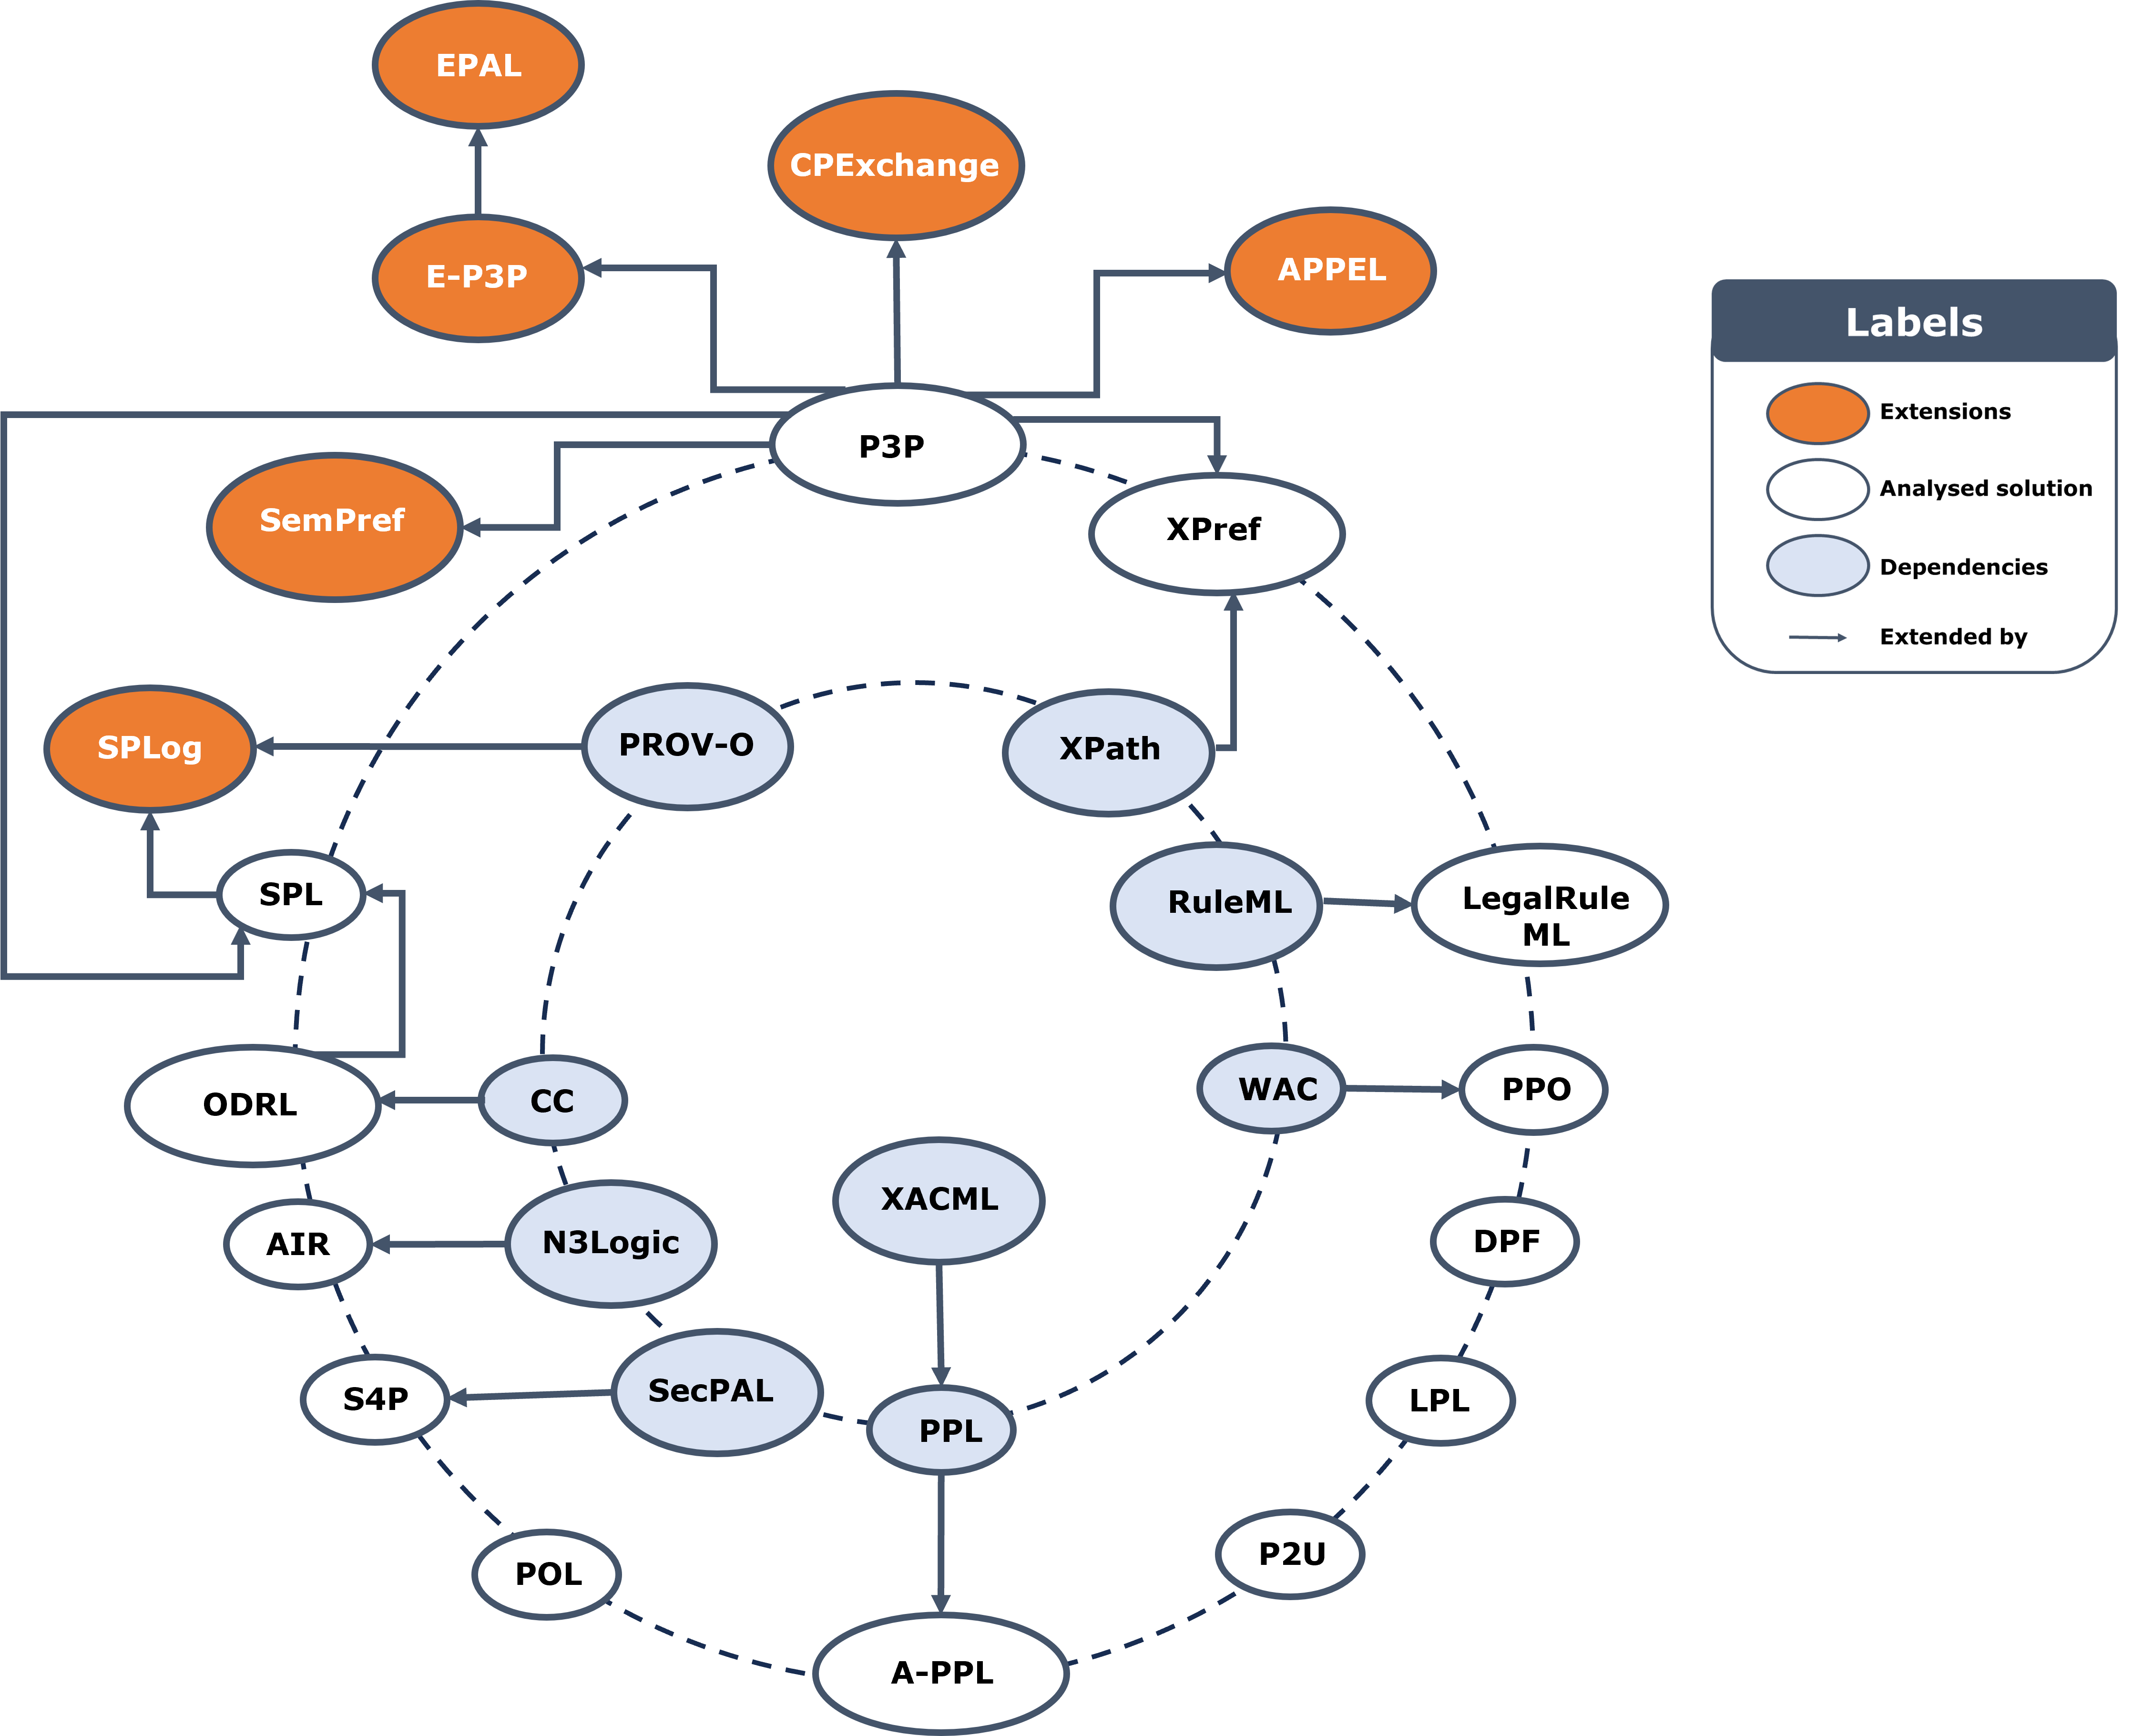
\includegraphics[width=\textwidth]{figures/chapter-2/languages.png}
    \caption{Privacy-related policy languages dependency chart.}
    \label{fig:lang-dependency-graph}
\end{figure}

Moreover, the following criteria were used to analyse existing research on semantic policy languages:
\begin{enumerate}
    \item[(C1)] Ability to model deontic concepts, e.g., permissions, prohibitions, obligations.
    \item[(C2)] Ability to model GDPR concepts, such as the privacy terms in Table~\ref{tab:GDPR_privacy_terms}.
    \item[(C3)] Existence of taxonomies of terms to populate policy conditions.
    \item[(C4)] Existence of mechanisms to assist with compliance.
    \item[(C5)] Resource is maintained/continues to be actively developed.
    \item[(C6)] Existence of an open and accessible specification.
\end{enumerate}

The outcomes of this comparative analysis will be provided in Section~\ref{sec:sota_policies_analysis} and systematised in Table~\ref{tab:languagesComparison}.

\subsection{Semantic policy languages for access control}
\label{sec:sota_policies_description}

This Section's main goal is to describe existing policy languages related to privacy, delineating the structure and information offered by each language.
Additionally, their compatibility with the GDPR is assessed, focusing on their ability to describe the provisioned rights and obligations.
Moreover, Table~\ref{tab:resources-policy-languages} provides an overview of these languages and collects information about the creators of the resources, their versions, the date of publication, and the date of the last known update.
Said languages are then analysed in chronological order regarding the date of publication and a dependency graph is presented in Figure~\ref{fig:lang-dependency-graph}.

To complement the description of the languages presented in this Section, additional documentation and resources were published on a Web page\footnote{Available at \url{https://w3id.org/people/besteves/phd/sota/languages}. Its public repository can be consulted at \url{https://w3id.org/people/besteves/phd/sota/repo} for further improvement when new solutions appear.}, including diagrams and code examples.

\subsubsection{P3P}
\label{sec:p3p}

\cite{cranor_platform_2002} introduced the Platform for Privacy Preferences (P3P) language as a standard for Web services to disclose their privacy practices in a machine-readable format.
This facilitated user agents in easily interpreting these practices and notifying users about decisions based on them. 
However, despite enabling users to be informed about the privacy policies of Web pages, these mechanisms do not ensure that the pages are actively adhering to these policies, as P3P lacks enforcement capabilities.
Therefore, the P3P vocabulary was designed not to comply with a specific regulation but rather to specify the practices of single Web pages.

The primary contributions of the P3P specification include a data schema for outlining the data intended to be collected by the Web page, a standardised set of purposes, data categories, and recipients, and an XML standard for defining privacy policies.
P3P policies consist of both general assertions and specific statements, the latter being related only to certain types of data.
General assertions encompass the legal entity applying the policy and informational elements related to access, disputes, and remedies.
The access element indicates whether the Web page allows access to the data it gathers and the disputes element outlines a process for resolving privacy-related disputes, while the remedy element details potential solutions in the event of a policy breach.
Additionally, each P3P statement consists of a distinct `data group' containing one or more data elements, along with purpose, recipient types, and retention elements.
In this context, P3P outlines a range of purposes relevant to Web-based data processing operations, such as facilitating and supporting the initial activity for which the data was supplied, conducting research and development, or performing data analysis.
%The purpose element is required to include at least one specification of purpose.
The recipient type element can be used to specify who will benefit from the collected data, while the retention element must accurately reflect the policy regarding how long the data will be kept.
Listing~\ref{list:p3p_example} displays a P3P policy that underscores the aforementioned P3P elements.
CatalogExample gathers essential details concerning its users' computer systems, as well as data regarding the pages they visit.
This information serves system administration and research and development purposes and is exclusively utilised by the company and retained for a duration deemed suitable for the specified purposes.

\begin{listing}
\caption[P3P privacy policy.]{P3P policy extracted from Example 3.1 of the P3P specification~\citep{cranor_platform_2002}, which specifies the privacy policy of CatalogExample.}
\label{list:p3p_example}
\begin{minted}{turtle}
<http://example.com/#forBrowsers> a p3p:Policy ;
    p3p:disclosure <http://example.com/PrivacyPractice.html> ;
    p3p:entity [
        p3p:business.name [ rdf:value "CatalogExample" ] ;
        p3p:business.contact-info.postal.street [
            rdf:value "4000 Lincoln Ave." ] ;
        p3p:business.contact-info.postal.city [
            rdf:value "Birmingham" ] ;
        p3p:business.contact-info.postal.stateprov [ rdf:value "MI" ] ;
        p3p:business.contact-info.postal.country [ rdf:value "USA" ] ;
        p3p:contact.online.email [ rdf:value "catalog@example.com" ] ;
        p3p:contact.telephonenum.intcode [ rdf:value "1" ] ;
        p3p:contact.telephonenum.loccode [ rdf:value "248" ] ;
        p3p:contact.telephonnum.number [ rdf:value "3926753" ] ] ;
    p3p:access p3p:AccessClass-nonident ;
    p3p:statement [
        p3p:purposeAlways p3p:Purpose-admin, p3p:Purpose-develop ;
        p3p:recipientAlways p3p:Recipient-ours ;
        p3p:retention p3p:Retention-stated-purpose ;
        p3p:data [
            rdf:predicate p3p:dynamic.clickstream, p3p:dynamic.http ] ] .
\end{minted}
\end{listing}

P3P was initially developed to articulate policies of Web services, prompting the design of APPEL as an extension to empower users in expressing their preferences~\citep{cranor_p3p_2002}.
Consequently, the utilisation of both languages becomes imperative to align user privacy preferences with service privacy policies.
Furthermore, \cite{bohrer_customer_2000} introduced the CPExchange language, an XML specification facilitating the transfer of customer data across enterprise services, incorporating P3P privacy policies relevant to the exchanged data.
Likewise, EPAL~\citep{ashley_enterprise_2003}, developed by IBM Research\footnote{\url{http://www.research.ibm.com/} (accessed on 16/July/2023)} along with its precursor E-P3P~\citep{ashley_e-p3p_2002}, leveraged P3P statements to align enterprise privacy policies with user preferences.
\cite{li_semantics-base_2006} introduces a declarative data-centric semantic model alongside a succinct syntax for P3P policies, facilitating the representation of the relationship between various P3P elements.
The primary aim of this language is to articulate policies in a manner that can be uniformly interpreted and represented across diverse user agents.
Extending this semantic foundation, the authors put forward SemPref, a preference language that considers the significance of the privacy policy rather than its syntactic form.

The P3P 1.0 Specification achieved W3C Recommendation status on April 16, 2002.
Nonetheless, its adoption was restricted as it requires acceptance from both Web services and users.
Furthermore, there has been no protocol established for these P3P policies to accurately reflect the privacy practices of Web pages.
While this specification did attain W3C recommendation status, its failure to gain widespread adoption rendered it obsolete by 2018.
Nonetheless, the significance of P3P remains considerable, as its inception and utilisation marked a pioneering endeavour in the realm of machine-readable privacy languages. 
Consequently, the primary lessons derived from this language pertain to the necessity of establishing a formal semantics capable of delineating both data subject and controller policies, which accurately reflect their data preferences and practices, and the need for tools that effectively enforce the outlined policies.

\subsubsection{ODRL}
\label{sec:odrl}

The ODRL Vocabulary \& Expression 2.2~\citep{iannella_odrl_2018} gained W3C Recommendation status in February 2018, developed by the Permissions \& Obligations Expression Working Group, with its initial version launched back in 2001.
Its primary objective was to establish a language capable of translating natural language policies into machine-readable formats, specifying details regarding permissions, prohibitions, and obligations pertaining to an asset.
This vocabulary stems from the consolidation of previous efforts undertaken by the ODRL CG, encompassing the ODRL V2.1 Common Vocabulary, the ODRL V2.1 XML Encoding, the ODRL V2.1 Ontology, and the ODRL V2.1 JSON Encoding.
Ongoing maintenance of the ODRL's standards and specifications are supported by the ODRL CG.

ODRL includes two vocabularies for the description of policies: the ODRL Core Vocabulary and the ODRL Common Vocabulary.
The primary class within ODRL's Core Vocabulary is the `policy' concept, facilitating the identification of a specific policy through its unique identifier.
Within each policy, there may exist multiple rules -- an abstract class that outlines the shared characteristics of permissions, prohibitions, and duties.
These rule types serve to declare whether a particular action, e.g., over as asset, is permitted, prohibited, or obligatory.
Additionally, permissions might also be linked with duties that must be fulfilled for said permissions to be active.
Furthermore, rules undergo further refinement through the usage of constraints, which specify the circumstances under which the rule applies, e.g., a particular permission remains valid until the conclusion of 2024.
The ODRL Vocabulary also outlines a collection of 49 actions, nine of which are imported the Creative Commons (CC) vocabulary.
The entities, or parties, involved (which can encompass a group of individuals, an organisation, or an agent) are responsible for enforcing the rules and may assume various roles contingent upon their relationship with the asset, e.g., the entity issuing the rule adopts the assigner role, whereas the recipient of the rule assumes the assignee role.
An asset, on the other hand, refers to an identifiable resource, such as data, software, services, or a combination thereof, that is subject to a rule.
The ODRL Common Vocabulary further delineates subclasses of policies, roles played by the involved parties, taxonomies of use and transfer actions for rules, and a variety of constraint operands, such as temporal, spatial, or sector-specific.
Of particular significance concerning the GDPR is the privacy policy subclass regarding assets containing personal data. 
Consequently, privacy policies implementing the ODRL language must specify to the involved parties the manner in which data is utilised, as well as with whom and for what purpose.
Listing~\ref{list:odrl_example} provides an implementation of an ODRL privacy policy that underscores the aforementioned elements, including a duty for the assignee to be allowed to use the data and a consequence in case they do not.

\begin{listing}
\caption[ODRL privacy policy.]{ODRL \texttt{Privacy} policy.}
\label{list:odrl_example}
\begin{minted}{turtle}
<http://example.com/privacy-policy> a odrl:Privacy ;
    odrl:uid <http://example.com/privacy-policy> ;
    odrl:permission [
        odrl:target <http://example.com/beatriz/contacts> ;
        odrl:assignee <http://example.com/beatriz> ;
        odrl:assigner <http://example.com/company-a> ;
        odrl:action odrl:use ;
        odrl:duty [
            odrl:action odrl:obtainConsent ;
            odrl:consentingParty <http://example.com/beatriz> ;
            odrl:consequence [
                odrl:assigner <http://example.com/company-a> ;
                odrl:action odrl:delete ] ] ] . 
\end{minted}
\end{listing}

ODRL's representational capabilities exhibit some limitations, as highlighted by~\cite{kebede_critical_2020}, particularly regarding the portrayal of delegation, the various semantics utilised for expressing duties, and the management of conflicts.
Nevertheless, efforts such as those described by~\cite{fornara_operational_2018, fornara_using_2019} are underway to formalise the semantics of ODRL policies.

ODRL was applied in various contexts, including its usage by working groups within the Open Mobile Alliance SpecWorks\footnote{\url{https://www.omaspecworks.org/} (accessed on 18/July/2023)} and by the IPTC Rights Expressions WG for the RightsML Standard\footnote{\url{https://www.iptc.org/std/RightsML/2.0/RightsML_2.0-specification.html} (accessed on 18/July/2023)}.

\subsubsection{XPref}
\label{sec:xpref}

\cite{agrawal_xpref_2005} introduced XPref as an alternative to APPEL, which only permits the definition of P3P policies that are not allowed by the user.
XPref utilises XPath (XML Path Language) 1.0 and 2.0 expressions to replace APPEL rules, enhancing the precision and reducing errors in policy formulation.
Both XPath 1.0, as described by~\cite{clark_xml_1999}, and XPath 2.0, as detailed by~\cite{berglund_xml_2010}, attained W3C Recommendation status on November 16th, 1999, and December 14th, 2010, respectively.
It should be noted that these specifications are no longer subject to further maintenance since subsequent versions have been developed.
In this context, the primary objective of XPath is to offer a method for traversing the hierarchical elements within an XML document.
In pursuit of this objective, XPath views an XML document as a tree structure of nodes
When an XPath expression is applied to the document, it determines an ordered sequence of nodes, resulting in a concise path representation.
This path consists of expressions that yield various types of nodes, including root, element, text, attribute, namespace, processing instruction, or comment nodes.

XPref was crafted to ensure that its rules not only recognise combinations of P3P elements that render a policy unacceptable based on user preferences, but also confirm that the presented elements are defined as acceptable.
It achieves these objectives while preserving the syntax and semantics of APPEL, along with its core classes.
However, the contents of the rules are substituted with XPath expressions, given that P3P policies are XML documents and can thus be readily compared with XPath-based rules.
These expressions are defined by appending a `condition' attribute to the rule, which activates the rule when the XPath expression yields a non-empty result.
%Consequently, utilising the `behavior' attribute in XPref rules allows for preferences to be set to either permit or restrict services based on the P3P policy elements they contain, such as purposes and recipients, specified in the "condition" attribute.

\subsubsection{AIR}
\label{sec:air}

In 2010, \citeauthor{hitzler_analyzing_2010} developed Accountability in RDF (AIR) -- a declarative language enabling the assertion of facts and the inclusion of rules.
AIR is built on N3Logic~\citep{berners-lee_n3logic_2008}, which supports rule nesting, rule reuse, and automated explanations of actions carried out by the AIR reasoner. 
These explanations can be customised and, given that they may contain sensitive data like Personally Identifiable Information (PII), can be employed to ensure privacy.
For example, they can be utilised to conceal actions executed under specific rules.

N3Logic extends the RDF data model with the aim of expressing logic rules on the Web, thereby promoting the use of a unified language for both data representation and logical inference.
Thus, AIR leverages N3Logic's inherent capabilities, including built-in functions, nested graphs, and contextualised reasoning.
This enables AIR rules to incorporate the usage of graphs as literal values, and built-in functions or operators defined as RDF properties.

Each AIR rule is assigned a unique IRI, ensuring its seamless integration with the linked data cloud and facilitating its reuse.
These rules adhere to the following structure: \texttt{air:if} \texttt{condition}; \texttt{air:then} \texttt{then-actions}; \texttt{air:else} \texttt{else-actions}.
The action instances can include annotations using the \texttt{air:description} property.
These annotations are subsequently integrated by the AIR reasoner into its justifications and can serve to conceal PII found within the rules.
Additionally, the format of the rules graph permits the nesting of rules within the same rule set.
This feature offers a means to segment the conditions outlined by the rule, allowing only a portion of them to be revealed in the justifications.

\subsubsection{S4P}
\label{sec:s4p}

S4P (SecPAL for Privacy), designed by \cite{becker_framework_2009, becker_s4p_2010}, constitutes a language framework designed for articulating users' privacy preferences and the data handling practices of Web services. Originating from Microsoft Research\footnote{\url{https://www.microsoft.com/en-us/research/} (accessed on 16 March 2024)}, this language serves as an extension of the company's earlier endeavor, SecPAL, aimed at delineating PII management.

SecPAL \citep{becker_design_2007} is a flexible, decentralised authorisation language, crafted for articulating policies and enhancing their expressiveness to define delegation conditions, domain-specific constraints, and negation.
An authorisation policy comprises a set of assertions, each associated with an issuer responsible for vouching for the assertion, along with a collection of conditional facts and constraints pertaining to temporal or spatial aspects.
Subsequently, when an access request is made, it undergoes a transformation into a series of queries.
These queries are then matched against the clauses that represent the system's policies, ultimately leading to a decision on data access conditions.
S4P extends SecPAL by treating granted rights and required obligations as assertions and queries.
Based on these, a satisfaction checking algorithm is formulated to evaluate the disclosure of PII between users and data-collecting services.
As a result, services should articulate their data-handling practices in the form of SecPAL queries.
Conversely, users specify their preferences as SecPAL assertions, precisely delineating what services are authorised to do and what duties they have regarding r=the usage of said PII.
% The satisfaction algorithm evaluates whether the data collection practices of the services align with the behaviors permitted by the users and whether the obligations specified in the users' preferences are adhered to by the services' policies.
If the algorithm yields a positive result, indicating that the service's policies complies with the user's preferences, the service can proceed with its data handling activities.
Additionally, S4P establishes a data disclosure protocol to ensure that users' preferences are respected when their data is shared with third party recipients.
% This protocol permits the disclosure of the user's PII only if the service's policies satisfy the user's preferences and if the policies of the third parties are in harmony with the user's preferences.

In addition to possessing an XML schema for implementation purposes, S4P features a human-readable and unambiguous syntax, enabling its utilisation in various applications. 
Listing~\ref{list:s4p_example} illustrates the S4P syntax in a scenario where Alice, the user, delineates her privacy preferences concerning the collection of her email address. 
Specifically, Alice permits eBooking services to utilise her email address for sending confirmations, newsletters, and for statistical purposes.
Additionally, Alice authorises the booking services to share her email address with trusted partners exclusively to engage with registered services that commit to deleting her email address within a month.

\begin{listing}
\caption[S4P instantiation.]{S4P example, extracted from \cite{becker_framework_2009}, which specifies Alice's privacy preferences concerning the collection of her email address by eBooking services.}
\label{list:s4p_example}
\begin{minted}[escapeinside=||]{python}
Alice says x may use Email for p if
    x is a eBookingService,
    where p |$\in$| {Confirmation, Newsletter, Stats}
Alice says x may send Email to y if
    x is a eBookingService,
    y is a TrustedPartner
Alice says x can say y is a TrustedPartner if
    x is a eBookingService
Alice says |$\langle$|Service|$\rangle$| is a RegisteredService|$?$| |$\wedge$|
    |$\exists$|t (|$\langle$|Service|$\rangle$| says |$\langle$|Service|$\rangle$| will delete Email within t|$?$| |$\wedge$| t |$\leq$| 30 days|$?$|)
\end{minted}
\end{listing}

\subsubsection{POL}
\label{sec:pol}

The Privacy Option Language (POL) was formulated by~\cite{berthold_privacy_2013} to establish privacy contracts between data controllers and data subjects, drawing on the principles of financial option contracts and corresponding data disclosure agreements.
Its architecture enforces the `data minimisation' principle by converting privacy contracts into a standard format.
This standardised format ensures that variations in contract compositions are normalised, thus providing a consistent semantic structure across contracts.

Within POL, every privacy contract is dedicated to delineating the responsibilities and entitlements concerning data disclosure.
Given its origins in the financial sphere, contract constructions in POL primarily revolve around obligations, except when a straightforward formulation of such rule types is impractical.
To specify these formulations, POL relies on various modules that are also open to extension.
The language delineates key components, including the \textbf{syntax} module, alongside modules addressing \textbf{personal data}, \textbf{purpose}, \textbf{observable} values, and \textbf{time}.
Additionally, it includes semantics modules focusing on \textbf{management} and enhancing \textbf{human readability}.
The syntax module comprises language primitives essential for defining POL contracts in their standard format.
These contracts can then integrate with data modules through various data support structures, ranging from basic attribute-value pairs, e.g., \textit{(eye colour, brown)}, to intricate tree-like data structures.
More specifically, the observable module defines comparison and Boolean operators, which are accessible within the contract execution environment, facilitating evaluations related to e.g. data retention periods.
The time module can be used to formalise different time restrictions, e.g. event-driven, discrete, or continuous time.
Furthermore, semantic modules are utilised for managing changes in observable variables, e.g., when time elapses, and for translating POL contracts into natural language.
Listing~\ref{list:pol_example} showcases the semantics of POL through a list of contracts examples:
(1) Contract $c_{company}$ delineates the immediate usage of personal data $a_1$ for purpose $p_1$;
(2) $c_{user}$ represents the negation of $c_{companyA}$ and pertains to the user disclosing the data;
(3) $c_A$ signifies a contract wherein a company holds the right to utilise data $a_A$ for purpose $p_A$ at time $t_A$ or can opt not to use it at all (represented by the $zero$ variable in the contract instantiation); and
(4) $c_B$ denotes a scenario where a company may or may not utilise data $a_B$ for purpose $p_B$ until time $t_B$ and is obligated to delete it after the deadline $t_B$.

\begin{listing}[ht]
\caption[POL contracts.]{POL contracts extracted from~\cite{berthold_towards_2011}.}
\label{list:pol_example}
\begin{minted}[escapeinside=||]{text}
(1) |$c_{company}$| = data |$a_1$| |$p_1$|
(2) |$c_{user}$| = give |$c_{company}$|
(3) |$c_A$| = when (at |$t_A$|) (data |$a_A$| |$p_A$| |`or'| zero)
(4) |$c_B$| = until (at |$t_B$|) (data |$a_B$| |$p_B$| |`or'| zero) 
\end{minted}
\end{listing}

The development of this language took place within the PETWeb II project, primarily aimed at tackling societal inquiries within the electronic identifiers domain.
The online documentation offers various application scenarios illustrating POL's utilisation.

\subsubsection{PPO}
\label{sec:ppo}

The Privacy Preference Ontology (PPO)~\citep{sacco_privacy_2011} proposes a framework for expressing users' privacy preferences regarding the restriction or allowance of access to particular RDF statements within a document.
This ontology expands upon WAC to determine users' data access rights, which is limited to specifying who can access an entire RDF document, by allowing finely-grained mechanisms for governing users' access to specific data within RDF resources.

PPO's capabilities for imposing access restrictions extend to individual statements, statement groups, and resources, which can be specific subjects or objects within RDF triples. 
Additionally, it is essential to specify the type of restriction, as users may be granted either read, write, or both access modes to the data.
By utilising the designated \textbf{hasCondition} property, specific conditions can be established to delineate privacy preferences concerning particular resources, instances of specific classes or properties, or even specific property values.
%Furthermore, it's imperative to define the access criteria to ensure that users fulfill the necessary requirements to access certain resources.
These conditions can then be checked against a SPARQL ASK query containing all the attributes and properties that users must satisfy to allow or deny access to data.

The authors also created a dedicated privacy preference manager~\citep{sacco_privacy_2011b} based on PPO.
The objective was to empower users to articulate their individual privacy preferences and manage data access based on profile attributes such as relationships, interests, or other shared characteristics.
% This ontology has the versatility to encompass social data modeled in RDF or facilitated via RDF wrappers, which can be integrated into various web pages using their Application Programming Interface (API).

\subsubsection{LegalRuleML}
\label{sec:legalruleml}

LegalRuleML, a rule language tailored to the legal domain, is developed and maintained by the OASIS\footnote{OASIS is a non-profit organisation that focuses on open standards for cloud, security and other domains, \url{https://www.oasis-open.org/} (accessed on 18/July/2023).} LegalRuleML Technical Committee and it attained OASIS Standard status in August 2021~\citep{palmirani_legalruleml_2021}.
This XML-schema specification builds upon and extends RuleML~\citep{boley_specification_2017} and incorporates formal features to represent and facilitate reasoning over legal norms, guidelines, and policies.
Key attributes of LegalRuleML include the utilisation of multiple semantic annotations for various legal interpretations, deontic operators, temporal rule management and tracking, and a mapping to RDF.

Hence, the fundamental components of a LegalRuleML document encompass \textbf{metadata}, \textbf{context}, and \textbf{statements}. 
The metadata segment comprises details concerning the \textbf{legal source} of the norms, ensuring their linkage with the corresponding legal text statements.
Additionally, it includes information about the \textbf{actors} and their \textbf{roles} in relation to the established rules, the \textbf{jurisdiction}, the \textbf{authorities} responsible for rule creation, endorsement, and enforcement, as well as temporal parameters defining rule validity.
The context element facilitates the expression of varying interpretations of rule sources, which may evolve over time or differ across jurisdictions.
It also facilitates the representation of the \textbf{association} element, establishing connections between legal sources and rules.
The statements segment involves the formalisation of norms, encompassing constitutive and prescriptive statements, as well as override and violation-reparation statements.
Constitutive rules encapsulate definitions outlined in legal documents, whereas prescriptive rules encode deontic specifications.
Override statements serve to address conflicting rules, while violation and reparation statements formalise penalties for breaches of norms.

Specifically, \cite{palmirani_modelling_2018} introduced a framework that leverages LegalRuleML, Akoma Ntoso, and the PrOnto ontology (outlined in Section~\ref{sec:pronto}) to model rules and verify compliance with GDPR's \textit{`Conditions applicable to child's consent in relation to information society services'}, described in Article 8~\citeyearpar{noauthor_regulation_2016}.

\subsubsection{A-PPL}
\label{sec:appl}

The Accountable Policy Language (A-PPL), developed by~\cite{azraoui_appl_2014}, originates from the A4Cloud\footnote{\url{http://www.a4cloud.eu/} (accessed on 19/July/2023)} project, aimed at incorporating accountability requirements into the expression of privacy policies.
To achieve this aim, A-PPL extends PPL (PrimeLife Policy Language) by integrating considerations for notification protocols, data storage and retention practices, and auditability guidelines.
PPL by~\cite{ardagna_primelife_2009} is an extensible, XACML-based \citeyearpar{parducci_extensible_2013} privacy policy language established in the context of the PrimeLife\footnote{\url{http://primelife.ercim.eu/} (accessed on 19/July/2023)} project -- XACML is an OASIS standard for access control policies that has been previously tested to deal with GDPR requirements related to consent~\citep{fatema_compliance_2017} and privacy by design~\citep{piras_defend_2019}.
The main concepts within PPL for articulating obligations consist of \textbf{triggers} and \textbf{actions}.
Triggers denote events that can undergo filtering based on specific conditions and are linked to an obligation.
These triggers are responsible for initiating actions by the data controller, which are executed in accordance with the data subject's permissions.
However, neither PPL nor XACML encompass concepts that address needs such as representing information concerning data storage and retention restrictions or incorporating auditability conditions to align with personal data protection regulations.

A-PPL incorporated a role attribute identifier and introduced the role of data protection authority to those already present in PPL, namely the data subject, data controller, and data processor.
Additionally, two new triggers for permitting or denying access to personal data were incorporated.
Duration and location attributes pertaining to specific processing activities are utilised to enforce data retention and storage rules.
Furthermore, A-PPL extends the PPL notification system by specifying the recipient and notification type to be dispatched concerning a particular action.
To facilitate auditing, A-PPL introduced a trigger to oversee the data controller's activities and gather evidence of data-related occurrences, which are logged along with parameters such as the activity's purpose, timestamp, or the executed processing operation.
Listing~\ref{list:appl_example} showcases an instance of an A-PPL obligation to inform a data subject in the event of a personal data breach -- the $ActionNotify$ element offers a mechanism for notifying data subjects, triggered in instances of policy violations or data loss.

\begin{listing}[ht]
\caption[A-PPL policy.]{A-PPL example adapted from \cite{azraoui_appl_2014}.}
\label{list:appl_example}
\begin{minted}{xml}
<Obligation>
    <TriggersSet>
        <TriggerOnPolicyViolation/>
        <TriggerOnDataLost/>
    </TriggersSet>
    <ActionNotify>
        <Media>e-mail</Media>
        <Address>data-subject@example.com</Address>
        <Recipients>Data subject</Recipients>
        <Type>Policy Violation</Type>
    </ActionNotify>
</Obligation>
\end{minted}
\end{listing}

\subsubsection{P2U}
\label{sec:p2u}

The work presented by \cite{iyilade_p2u_2014} in Purpose-To-Use (P2U) draws inspiration from P3P to construct a policy framework facilitating the sharing of user information across various services and data consumers, grounded in the principle of purpose-driven usage.
Its primary objective is to furnish a language tailored for secondary data sharing and usage, with an emphasis on safeguarding user privacy. 
P2U is structured to encompass details regarding the purpose of data sharing, its duration, and, if desired by the user, potential selling price, while also enabling data consumers to engage in negotiations concerning pricing and retention time.

This policy framework entails the interaction among distinct entities: \textbf{users} (who own the data), \textbf{data consumers} (services requiring the data), \textbf{data providers} (services gathering and sharing the data), and \textbf{data brokers} (services overseeing consumer and provider activities, including negotiation tasks).
Thus, the principal concepts of P2U are \textbf{policies}, \textbf{purposes}, \textbf{retention} restrictions, \textbf{data groups}, and their corresponding \textbf{data} elements, and the previously mentioned entities.
Policies serve as the foundational component of P2U, with each requiring an associated provider, user, and at least one designated purpose of use. 
In addition, every policy must be assigned a name and may optionally include an attribute indicating the path to a human-readable policy, as well as the name and identifier of the corresponding data provider and user. 
Within a P2U policy, multiple purposes for data sharing can be specified, along with details on retention duration, authorised recipients, and the pertinent data involved. 
Moreover, the data consumer element includes a \textbf{name} property which can be designated as `public' to allow data sharing with any third-party service. 
The duration of each purpose's retention period should be defined in days, and an optional \textbf{negotiable} property, which defaults to false, can be specified (this term can also be applied to the data group element).
The data group component comprises one or more data elements, each capable of being assigned an expiry date, which takes precedence over the retention period of the period, and the option to specify an initial price for the data, should the user opt to sell it.
Listing~\ref{list:p2u_example} illustrates an instance of a secondary data sharing P2U policy -- the data provider ``FoodIntakeApp'' wants to share Jerry's data with the data consumer ``MyShopApp'' for the purpose of shopping recommendations, allowing the consumer to retain the data for a period of 180 days and to negotiate terms with the provider.

\begin{listing}
\caption[P2U policy.]{P2U example adapted from \cite{iyilade_p2u_2014}.}
\label{list:p2u_example}
\begin{minted}{xml}
<POLICY discuri=http://mydatawebsite.com/privacy.html name="ShoppingPolicy">
    <PROVIDER name="FoodIntakeApp" provid="p6528m2" />
    <USER name="Jerry" userid="u1030050503050" />
    <PURPOSE name="Shopping Recommendations" puid="102">
        <CONSUMER name="MyShopApp" consid="c10023" />
        <RETENTION period="180" />
        <DATA-GROUP groupid="g090353" negotiable="TRUE">
            <DATA ref="#dailyfoodintake.food" sell="FALSE" />
            <DATA ref="#dailyfoodintake.quantity" sell="FALSE" />
            <DATA ref="#dailyfoodintake.hungerscale" sell="FALSE" />
        </DATA-GROUP>
    </PURPOSE>
</POLICY>
\end{minted}
\end{listing}

Another publication by the same authors~\citep{hutchison_framework_2013} outlines a scenario where a user permits data sharing among multiple mobile applications.
However, this implementation does not mandate data consumers to adhere to user-defined policies nor does it delineate any particular handling protocols for sensitive data.


\subsubsection{SPECIAL}
\label{sec:special}

The EU H2020 Scalable Policy-awarE linked data arChitecture For prIvacy, trAnsparency and compLiance (SPECIAL) project endeavoured to create technology that aids in navigating the contemporary tension between privacy and Big Data-based technologies.
As such, it aimed to furnish tools for data subjects, controllers, and processors, streamlining the management and transparent utilisation of such data.
As a result of this project, two vocabularies were developed: the SPL (SPECIAL Usage Policy Language) and the SPLog (SPECIAL Policy Log) vocabularies~\citep{gangemi_scalable_2018}.

A SPL usage policy delineates a collection of permissible actions aligned with the consent of the data subject.
To formalise these actions in accordance with GDPR requirements, SPL outlines five fundamental concepts: the \textbf{data} subjected to processing, the intended \textbf{purpose} of such processing, detailed information of the \textbf{processing} operation, information regarding \textbf{storage}, and the designated \textbf{recipients} of the processing outcomes. 
The data storage term encompasses the specification of two attributes: the storage location and duration.
Therefore, in mathematical terms, the usage policy is represented as a tuple consisting of five elements, each representing an instantiation of the five core classes, thereby defining a permitted activity.
Moreover, a composed usage policy can be formulated by joining a set of authorised processing activities.
The vocabularies crafted to delineate each concept within the SPL construct draw upon established privacy-related ontologies.
For instance, terms related to processing operations\footnote{\url{https://specialprivacy.ercim.eu/vocabs/processing\#} (accessed on 20/July/2023)} are derived from previous ontologies such as ODRL, while data categories\footnote{\url{https://specialprivacy.ercim.eu/vocabs/data\#} (accessed on 20/July/2023)}, recipients\footnote{\url{https://specialprivacy.ercim.eu/vocabs/recipients\#} (accessed on 20/July/2023)}, purposes\footnote{\url{https://specialprivacy.ercim.eu/vocabs/purposes\#} (accessed on 20/July/2023)}, storage duration\footnote{\url{https://specialprivacy.ercim.eu/vocabs/duration\#} (accessed on 20/July/2023)}, and location\footnote{\url{https://specialprivacy.ercim.eu/vocabs/locations\#} (accessed on 20/July/2023)} are derived from P3P.
These taxonomies have the potential for expansion through the introduction of additional sub-classes~\citep{bonatti_policy_2018}.
An example showcasing this extension possibility is illustrated in Listing~\ref{list:spl_example}, where the terms \texttt{HeartRate}, a sub-class of \texttt{svd:Health}, \texttt{Profiling} a sub-class of the processing term \texttt{svpr:Analyze}, and \texttt{Recommendation} as a subclass of the purpose \texttt{svpu:Marketing}, are introduced. 
In this example, data concerning heart rate and location are utilised for user profiling with the aim of generating recommendations, while the data is stored indefinitely within the servers of the data controllers situated in the EU and may be disclosed to any recipients.

\begin{listing}
\caption[SPL general usage policy.]{SPL general usage policy adapted from \cite{bonatti_special_2019}.}
\label{list:spl_example}
\begin{minted}{text}
ObjectIntersectionOf(
    ObjectSomeValueFrom( spl:hasData
        ObjectUnionOf( ex:HeartRate svd:Location ))
    ObjectSomeValueFrom( spl:hasProcessing ex:Profiling )
    ObjectSomeValueFrom( spl:hasPurpose ex:Recommendation )
    ObjectSomeValueFrom( spl:hasStorage
        ObjectIntersectionOf(
            ObjectSomeValuesFrom( spl:hasLocation
                ObjectIntersectionOf( svl:OurServers svl:EU ))
            DataSomeValuesFrom( spl:durationInDays
                DatatypeRestriction( xsd:integer
                    xsd:mininclusive "0"^^xsd:integer ))))
    ObjectSomeValueFrom( spl:hasRecipient spl:AnyRecipient ))
\end{minted}
\end{listing}

SPLog was developed to document the processing events associated with the consent actions granted by data subjects.
It leverages PROV-O~\citep{lebo_prov-o_2013} to incorporate provenance information into the log, aligning with the terminology established for the SPL vocabulary. 
The key concepts outlined by SPLog encompass the \textbf{log} itself and the corresponding \textbf{log entries}.
Each log is accompanied by metadata, including the software agent to which it pertains, while log entries provide details about individual events. 
These entries can be categorised into two types: policy entries, which are linked to consent forms and associated terms, and data events, e.g., processing or sharing activities. 
Additionally, these entries should encompass information regarding the involved data subject, event description, content, timestamps, and relevant datasets, facilitating the tracking of event provenance.
Hence, SPLog utilises the SPL vocabulary to instantiate the content of a log entry, which allows event grouping to enhance scalability~\citep{kirrane_transparency_2018}.

The SPECIAL framework found application across diverse sectors through various use cases: collaborating with \textit{Proximus}\footnote{\url{https://www.proximus.be/} (accessed on 20/July/2023)} to develop personalised tourist recommendations; partnering with \textit{Deutsche Telekom}\footnote{\url{https://www.telekom.com/en} (accessed on 20/July/2023)} to deliver traffic alert notifications; and working alongside \textit{Thomson Reuters Limited}\footnote{\url{https://www.thomsonreuters.com} (accessed on 20/July/2023)} to address anti-money laundering requirements.

\subsubsection{DPF}
\label{sec:dpf}

The Declarative Policy Framework (DPF), as documented by \cite{martiny_protecting_2018} and \cite{martiny_partial_2020}, was developed as part of the DARPA Brandeis program\footnote{\url{https://www.darpa.mil/program/brandeis} (accessed on 20/July/2023)}.
Its primary objective is to furnish a privacy policy framework grounded in ontology engineering principles and a formal theory of shareability.
DPF's policy engine utilises the ontology to delineate policy instantiations, which subsequently inform the generation of user interfaces. 
These interfaces are designed to empower non-technical users to generate, validate, and manage privacy policies, alleviating them from the intricacies of technical policy language formalisms.
Furthermore, DPF's engine is adaptable for integration into systems that support data request management and other Privacy Enhancing Technologies (PETs).

Thus, DPF employs a predefined ontology as a common data model to articulate a specific domain, facilitating the formulation of both permissive and prohibitive privacy policies. 
Each policy rule encompasses either an allowance or denial statement, necessitating an identifier, a description, an authority, designated data requesters, and the pertinent data affected by the policy, along with the timeframe of its effectiveness. 
In instances of permissive statements, there is the option to outline a set of constraints that dictate the circumstances under which data may be shared. 
The policy authority is responsible for assessing whether a given data request aligns with the established policies.
Consequently, each data request must include not only the requested data but also the consulted policy authority tasked with granting or denying access, as well as the request timestamp.
Subsequently, the request travels through the policy engine pipeline, and upon encountering a matching rule, the engine furnishes the decision along with the identifier and description of the corresponding rule.
If the request is authorised, the engine also provides the valid conditions under which it is permissible. 
Given that a single request may trigger multiple policy rules, the engine must effectively manage conflicting decisions.
To address this, DPF incorporates baseline policies, and exceptions are established to delineate policy rules with higher priority concerning the shared data. 
Through this mechanism, this privacy framework is capable of overriding decisions based on specific constraints.

The ontologies are specified in OWL and can be converted to Flora\footnote{\url{http://flora.sourceforge.net/} (accessed on 20/July/2023)}, an object-oriented reasoning system. 
To demonstrate this framework, the authors offer a pandemic use case wherein national and community policy authorities establish data-sharing policies concerning their residents' health statuses to monitor disease outbreaks. 
In Listing~\ref{list:dpf_example}, an example DPF policy rule is provided based on this scenario.
Any national policy authority, $?pa$, permits nations to share information regarding their residents' disease states, $?reqData$, with response coordinators, $?requester$, at a specified time, $?time$, subject to certain constraints, $?constr$. 
The $?polData$ query delineates the relationship between nations and the medical statuses of their residents, constrained by $?constr$, which is attached to the $?Resident$ variable.
Within this constraint, the birthday of the resident is considered to exclude residents younger than thirteen from the requested data.

\begin{listing}[ht]
\caption[DPF policy.]{DPF constrained policy rule adapted from \cite{martiny_protecting_2018}.}
\label{list:dpf_example}
\begin{minted}[escapeinside=||]{text}
@!{NationsAllowConstrainedDiseaseStatesToRCs}
?pa [allow_sa(?requester, ?reqData, ?time, ?constr, ?id, ?descr, 0)] :-
    ?id = "NationsAllowConstrainedDiseaseStatesToRCs"^^\string,
    ?descr = "Nations share disease states w Response Coordinators"^^\string,
    ?pa : NationPolicyAuthority,
    ?requester : ResponseCoordinator,
    ?polData = |$\textdollar$|{ ?pa [nation -> ?Nation],
        ?Nation : Nation [community -> ?Community, name -> ?NationName],
        ?Community : Community [resident -> ?Resident],
        ?Resident : Person [medicalInformation -> ?MedInfo],
        ?MedInfo : DiseaseStatus [state -> ?MedState],
        ?Resident [constraints -> ?constr] },
    ?thirteenYears is 13*365*24*60*60, 
    ?time [subtractTime(?thirteenYears) -> ?latestTime],
    ?constr = [|$\textdollar$|{ 
        ?Resident : Person [birthDate -> ?Birthdate],
        timeBefore(?Birthdate, ?latestTime) }],
    implies_sharing(?polData, ?reqData, ?constr).
\end{minted}
\end{listing}

\subsubsection{LPL}
\label{sec:lpl}

The Layered Privacy Language (LPL), as developed by~\cite{gerl_lpl_2018}, is a privacy language designed to be comprehensible by both humans and machines.
Its primary objective is to facilitate the expression and enforcement of GDPR's requirements pertaining to data subject consent, personal data provenance, retention, and the implementation of privacy-preserving processing activities utilising advanced anonymisation techniques.
In subsequent research by~\cite{gerl_critical_2018}, efforts were directed towards enhancing LPL to comprehensively address the requirements outlined in Articles 12 to 14 of the GDPR, collectively known as the data subject's `Right to be informed'.

The policy structure of LPL is organised around purposes.
In this structure, a collection of \textbf{purposes} forms the core architecture, with each purpose being associated with a set of processed \textbf{data} types and their corresponding \textbf{recipients}.
Moreover, the purpose element can be enriched with a human-readable description and also includes properties such as \textbf{required}, which specifies whether a particular purpose needs explicit consent from the data subject, and \textbf{optOut}, indicating whether the user must actively accept or decline the purpose.
Data elements serve to identify the data group to which the processed data belongs, as well as categorise them as sensitive or explicit.
Alongside data recipients, other entities like data controllers or the data protection officer can also be designated with LPL.
Furthermore, LPL policies can include details on the retention period, data subject's rights, legal basis, and description details pertaining to automated decision-making activities.
The example LPL policy provided in Listing~\ref{list:lpl_example} illustrates how company $dr_{C1}$ operates its personal data handling activities under the LPL privacy policy $lpp_{ds_{U1}-dr_{C1}}$.
This policy governs the collection and usage of personal information from a user $ds_{U1}$ for a specific purpose $p_{U1}$.
Additionally, it allows for the optional sharing of collected data with a third-party recipient.
Should such sharing occur, a new contract must be established, with company $C1$ ($ds_{C1}$) acting as the data source and the third party $C2$ ($dr_{C2}$) as the data recipient.
The purpose of processing, denoted as $p_{U1}$, is `Marketing', involving personal data $\hat{D}_1$ such as postal code (anonymised via the `Suppression' method) and salary information, which must be deleted within 180 days following the fulfilment of the purpose.

\begin{listing}[ht]
\caption[LPL policy.]{LPL policy extracted from \cite{gerl_lpl_2018}.}
\label{list:lpl_example}
\begin{minted}[escapeinside=||]{text}
|$ds_{U1}$|=('U1','Person',|$publicKey_{U1}$|,'DataSource')
|$dr_{C1}$|=('C1','Legal Entity',|$publicKey_{C1}$|,'DataRecipient')
|$ds_{C1}$|=('C1','Legal Entity',|$publicKey_{C1}$|,'DataSource')
|$dr_{C2}$|=('C2','Legal Entity',|$publicKey_{C2}$|,'DataRecipient')
|$lpp_{ds_{U1}-dr_{C1}}$|=('1','LPP1','en','https://company.com/privacy.html',|$\emptyset$|,|$ds_{U1}$|,{|$p_{U1}$|})
|$p_{U1}$|=('Marketing','false','true','Marketing purposes, including newsletters.',{|$dr_{C1}$|,|$dr_{C2}$|},|$r_1$|,pm,|$\hat{D}_1$|)
|$r_1$|=('AfterPurpose','180 days')
|$\hat{D}_1$|={|$d_{postal}$|,|$d_{salary}$|}
|$d_{postal}$|=('postal-code',dGroup,'Number','true','Postal code of the user','QID',am1)
|$am_1$|=('Suppression',{|$ama_1$|,|$ama_2$|,|$ama_3$|,|$ama_4$|},|$\emptyset$|)
|$ama_1$|=('Suppression Replacement','*')
|$ama_2$|=('Suppression Direction','backward')
|$ama_3$|=('Minimum Level','2')
|$ama_4$|=('Maximum Level','4')
|$d_{salary}$|=('salary',dGroup,'Number','true','Monthly salary amount received by the user','Sensitive',|$\emptyset$|)
\end{minted}
\end{listing}

\cite{gerl_privacy_2019} conducted validation of this language through a real-world use-case scenario within the healthcare domain, showcasing its effectiveness and constraints concerning GDPR compliance.
Subsequent research expanded upon LPL by integrating machine-readable privacy icons~\citep{gerl_extending_2018}, aiming to evaluate their impact on the comprehension of privacy policies.
Additionally, an LPL Personal Privacy Policy User Interface was introduced~\citep{gerl_interface_2018}.
This interface primarily aims to present information pertinent to privacy policies, aiding data subjects in providing informed consent.
It includes a policy header containing a link to the human-readable policy and an overview of processing purposes using the previously mentioned privacy icons.
Furthermore, a purpose section outlines all purposes outlined in the privacy policy, along with details regarding data controllers, recipients, retention periods, and anonymisation methods.

\subsection{Comparative analysis}
\label{sec:sota_policies_analysis}

Using Table~\ref{tab:languagesComparison}, it is possible to assess and compare the policy languages outlined in this Section, regarding their effectiveness in aiding the representation of GDPR rights and obligations. 
The languages in the Table are arranged firstly by the number of supported criteria in descending order, followed by alphabetical sorting if needed, to enhance clarity and readability.

\begin{table}[ht]
\centering
\caption[Comparison of the analysed privacy policy languages.]{Comparison of the analysed privacy policy languages, according to the defined criteria described in Section \ref{sec:sota_policies_criteria}.}
\label{tab:languagesComparison} 
\begin{tabular}{ c||c|c|c|c|c|c}
 & C1 & C2 & C3 & C4 & C5 & C6 \\
 \hline\hline
 LegalRuleML & Yes & Partially & No & Yes & Yes & Yes \\
 \hline
 ODRL & Yes & Partially & Yes & No & Yes & Yes \\
  \hline
 SPL & No & Partially & Yes & Yes & No & Yes \\
 \hline
  A-PPL & Yes & Partially & No & Yes & No & No \\
 \hline
  DPF & Yes & Partially & No & Yes & Unknown & No \\
 \hline
  P3P & No & Partially & Yes & No & No & Yes \\
 \hline
  AIR & No & No & No & Yes & No & Yes \\
 \hline
  LPL & No & Partially & No & Yes & Unknown & No \\
  \hline
 S4P & No & Partially & No & Yes & No & No \\
 \hline
  P2U & No & Partially & No & No & No & No \\
 \hline
 POL & No & Partially & No & No & No & No \\
 \hline
  PPO & No & No & No & No & No & No \\
  \hline
 XPref & No & No & No & No & No & No \\
\end{tabular}
\end{table}

While these languages may not explicitly address the rights and obligations outlined in Section~\ref{sec:def_gdpr}, they can still encapsulate some of the information items discussed therein.
Thus, they are categorised as partially capable of representing GDPR concepts and principles (C2 criterion in Table~\ref{tab:languagesComparison}).
Most of the examined languages can partially fulfil the representational requirements of GDPR as identified in Table~\ref{tab:GDPR_privacy_terms}, with the exceptions being AIR, PPO, and XPref.
Examples illustrating how to encode specific aspects of privacy policies for each language partially capable of representing GDPR concepts are provided in Listings~\ref{list:p3p_example} to~\ref{list:lpl_example}.

Among these languages, only ODRL, SPL, and P3P offer taxonomies for populating policies.
Moreover, only LegalRuleML, ODRL, A-PPL, and DPF incorporate deontic concepts like permissions or obligations into their models.
In their documentation, LegalRuleML, SPL, A-PPL, DPF, AIR, LPL, and S4P also acknowledge the presence of reasoning mechanisms or other supportive tools, which leverage the implemented languages to aid in compliance efforts.
Some of these languages also provide access to such tools.
Nevertheless, LegalRuleML and ODRL are the only languages that are actively maintained and developed, while, among the languages examined, only LegalRuleML, ODRL, SPL, P3P, and AIR offer resources that can be readily reused on the Web.

Notably, LegalRuleML and ODRL distinguish themselves from other languages by possessing the capabilities to positively address a larger proportion of the established comparison criteria, including the ability to model deontic concepts and GDPR terms, e.g., purposes or data recipients.
Moreover, their development and extension can be supported by the community groups in charge of their maintenance, and their resources are open and accessible.
Beyond this, ODRL also supports the modelling of other constraints with particular importance in the definition of access control policies, e.g., spatial and temporal constraints, the representation of distinct types of policies, e.g., offers, requests and agreements, and has a profile mechanism to develop extensions to its core vocabulary.
As such, ODRL will be the basis upon which access policies are expressed in this Thesis.
\section{Gaps and challenges}
\label{sec:challenges}

This Section discusses the challenges of having a transparent, legally-aligned Solid ecosystem based on the literature review described in this Chapter. The following issues were identified based on the performed analysis:

\begin{enumerate} % copy from PLASMA paper
    \item [Ch1.] \textbf{Identity of Solid actors and their roles is unknown} -- Solid users are unaware of who are the entities providing and/or developing their Pods, the apps they use, WebIDs, or server infrastructure and implementation. Furthermore, most apps or services do not provide contact details or information regarding their data protection officer.
    \item [Ch2.] \textbf{No metadata about Solid infrastructure} -- Solid users do not have information on which Solid specification their Pod is running, which functionalities are installed within it or where are the servers located. Moreover, no record of this information is kept in the Pod for easy consultation by the user.\footnote{A non-exhaustive list of Pod providers is available at \url{https://solidproject.org/users/get-a-pod}, with information on the service used to host the Pods (but no information on the entities behind them) and, in some cases, the country where it is hosted (but no privacy policy for the storage service is provided).}
    \item [Ch3.] \textbf{Availability/Discovery of categories of data} -- To have granular access to data in Pods, based on their data category, Solid apps need to know if they exist and where are they stored in the Pod. Moreover, for seamless interoperability, schemas, formats or shapes for data recognised or supported by apps, services or Pods need to be recorded.
    \item [Ch4.] \textbf{Pod and app providers do not provide information on their data handling practices} -- Most providers and developers of Pod-related services do not provide human and/or machine-readable privacy notices nor do they declare what data they need to function. Such information also needs to be recorded in the Pod so that users can have a copy of the user/app request for data, e.g., in case data is used in a way that was not permitted by its data subject.
    \item [Ch5.] \textbf{Users cannot express their privacy policies} -- Solid users do not have the tools to express their privacy preferences and requirements nor to manage incoming data requests or existing decisions for the usage of data.
    \item [Ch6.] \textbf{No logging or record-keeping} -- No provenance metadata is recorded for accountability in the user Pod, e.g., users do not keep consent records, nor information regarding who has accessed their data, what they are doing with it, or changes to their data handling policies.
    \item [Ch7.] \textbf{No legal compliance checks} -- Solid does not provide its users with the tools to deal with legal requirements, such as giving/withdrawing consent or exercising rights under the GDPR, nor does it provide authorities with the auditing information to perform investigations.
\end{enumerate}

\chapter{Objectives and Contributions}
\label{chap:objectives}

\begin{figure}[p]
    \centering
    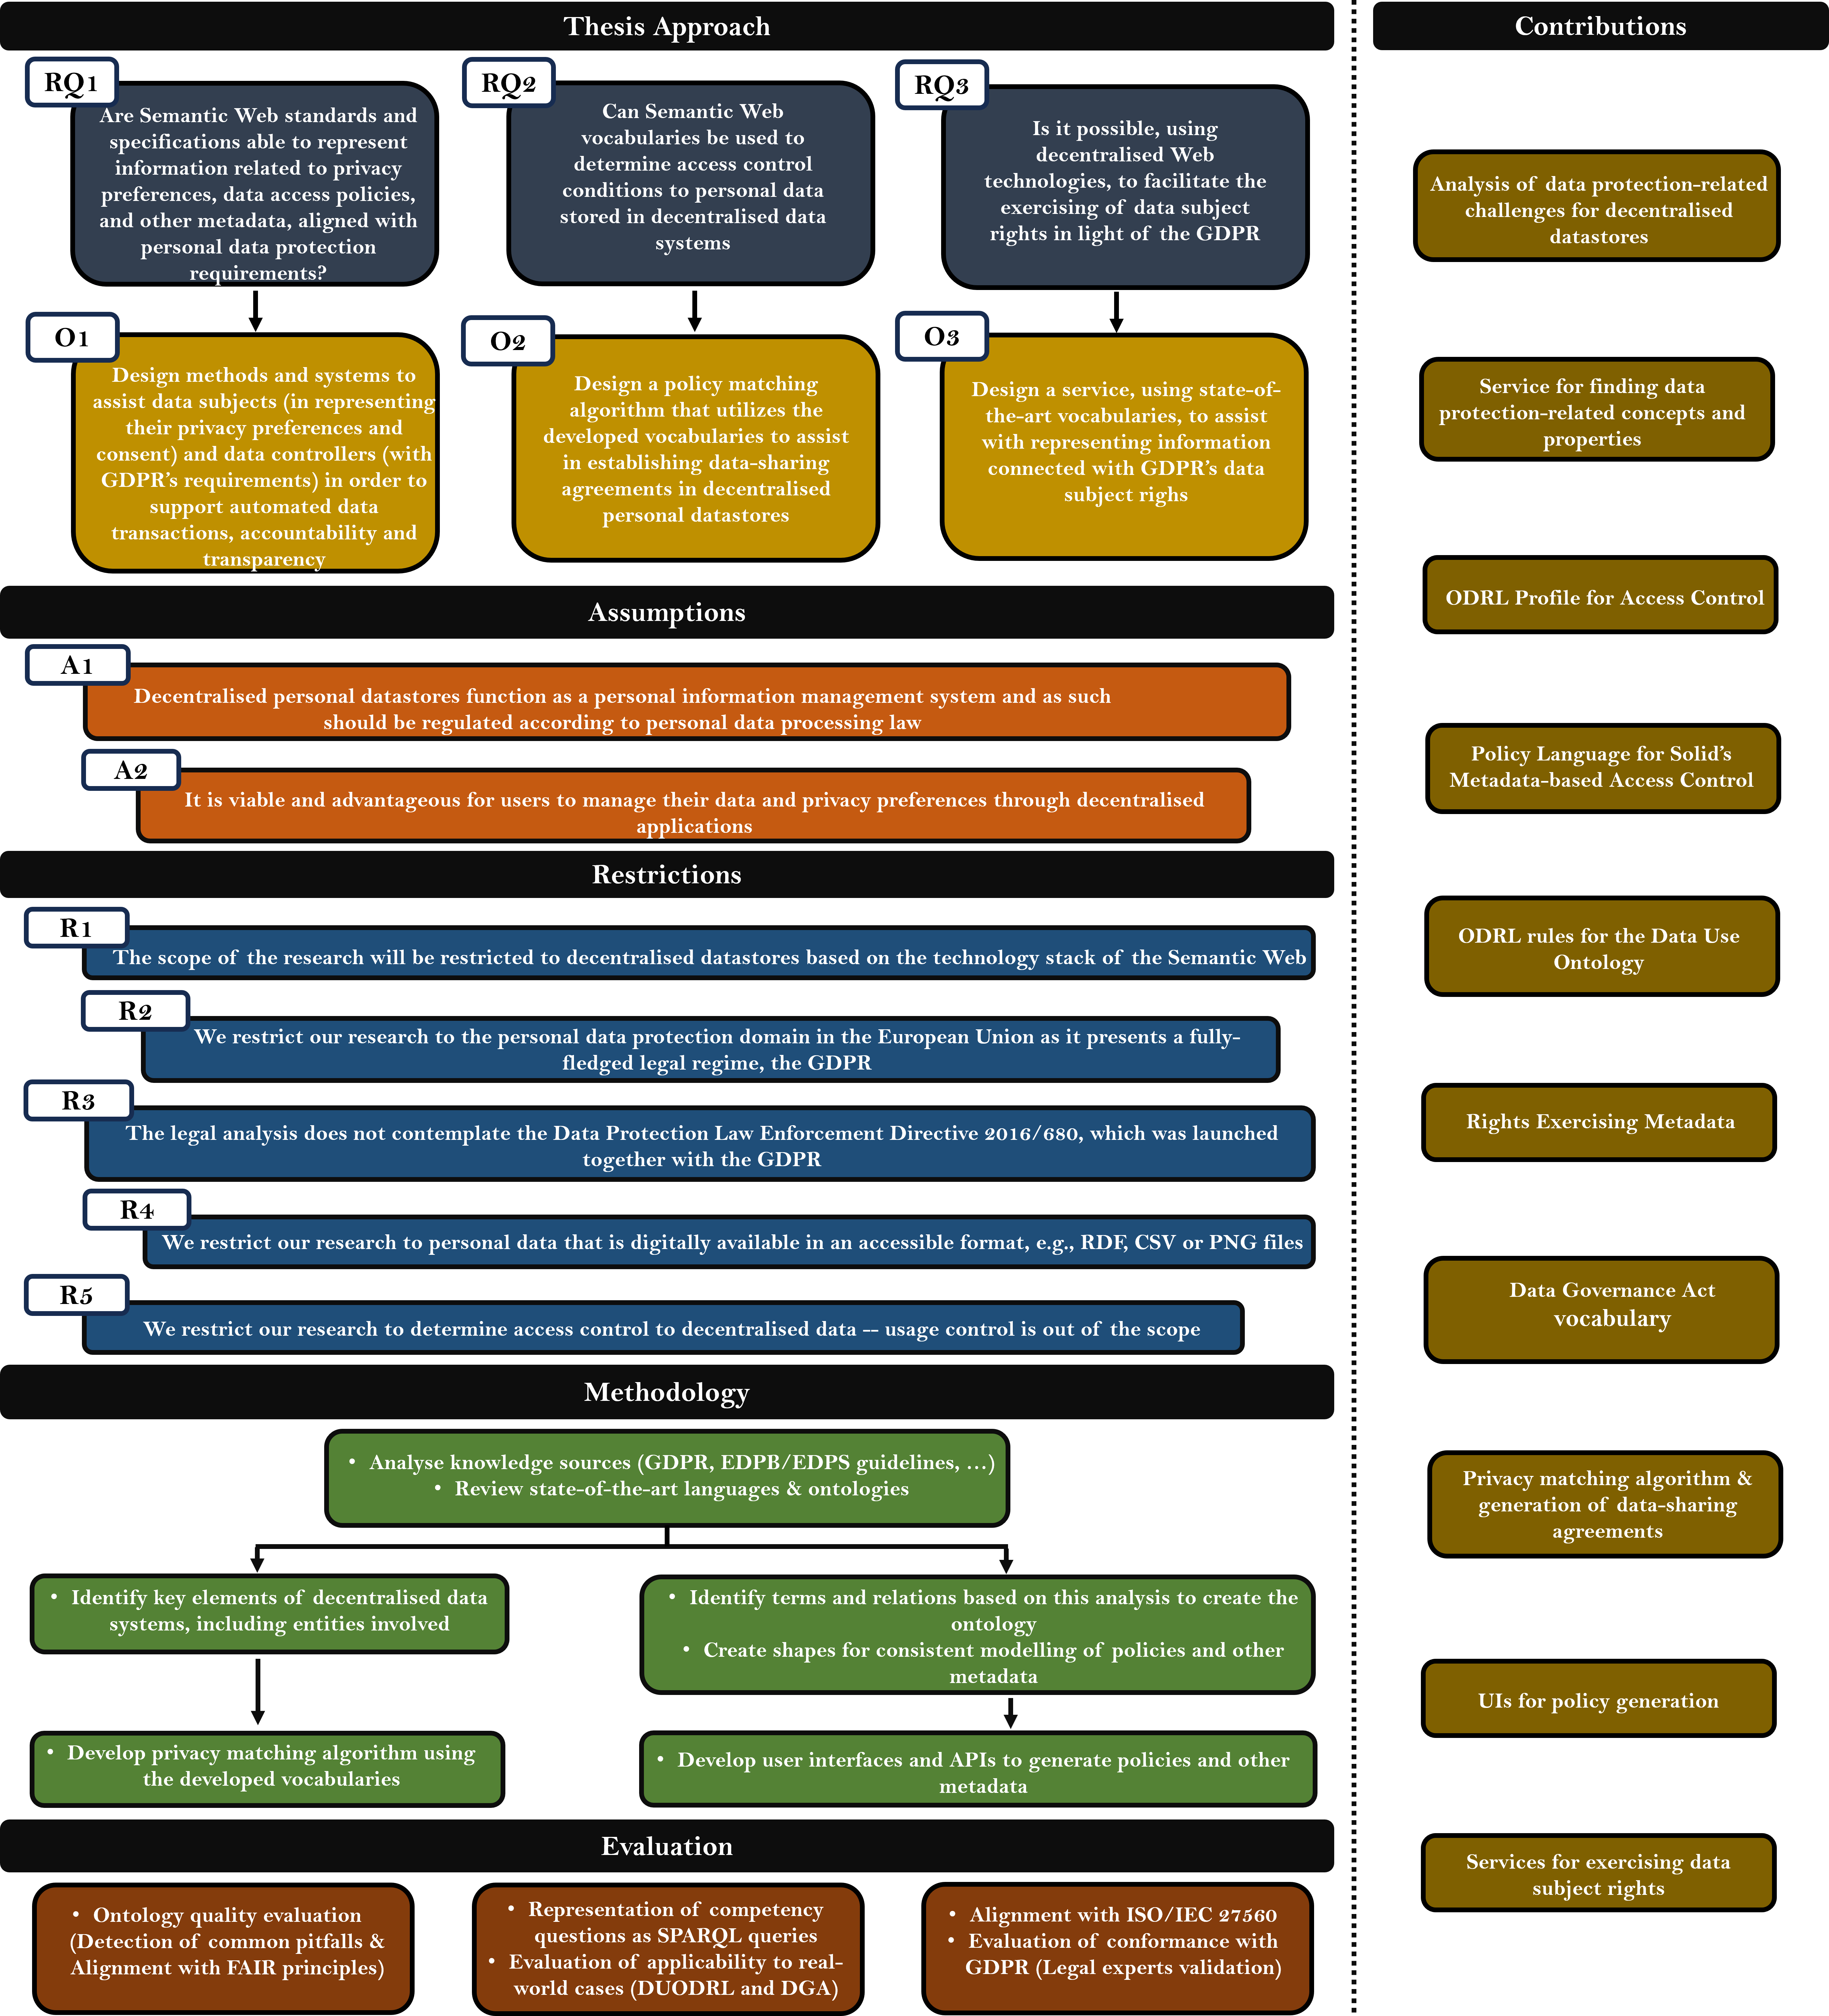
\includegraphics[width=1.1\linewidth]{figures/chapter-3/rqs_objs_diagram.png}
    \caption{Overview of the objectives and contributions of this Thesis.}
    \label{fig:objectives}
\end{figure}

\section{Objectives}
\label{sec:objectives}

To address the challenges and limitations identified in Section \ref{sec:challenges}, the main objective of this Thesis is the following:

\begin{tcolorbox}[colback=royallavender!20]
Research methodologies and design vocabularies and services to aid EU data subjects in taking control of the movement of their personal data.
\end{tcolorbox}

This main objective is divided into the following three sub-objectives:

\begin{enumerate}
    \item [\textbf{O1.}] Design methods and systems to assist data subjects (in representing their privacy preferences and consent) and data controllers (with GDPR’s requirements) in order to support automated data transactions, accountability and transparency.
    \item [\textbf{O2.}] Design a policy matching algorithm that utilises the developed vocabularies to assist in establishing data-sharing agreements in decentralised personal datastores.
    \item [\textbf{O3.}] Design a service, using state-of-the-art vocabularies, to assist with representing information connected with GDPR’s data subject rights.
\end{enumerate}

\section{Hypotheses}
\label{sec:hypotheses}

\begin{enumerate}
    \item [\textbf{H1.}] The use and extension of data protection vocabularies and machine-readable policy languages is suitable for the representation of consent terms and fine-grained policies for the processing of personal data.
    \item [\textbf{H2a.}] Data protection vocabularies and policy languages can be used to establish fine-grained access control conditions to personal data.
    \item [\textbf{H2b.}] Semantic Web vocabularies can be used to describe metadata related to decentralized personal datastores, including entities, infrastructure and roles.
    \item [\textbf{H2c.}] Data protection vocabularies can be used to represent machine-readable information related to data subject's rights.
    \item [\textbf{H3.}] Semantic Web vocabularies and decentralised technologies can be used as a basis for establishing a privacy matching process for the achievement of data-sharing agreements which fulfil the data subjects privacy preferences.
\end{enumerate}

\section{Assumptions}
\label{sec:assumptions}

The work presented in this Thesis is done under the following set of assumptions:

\begin{enumerate}
    \item [\textbf{A1.}] Decentralised personal datastores function as a personal information management system and as such should be regulated according to personal data processing law, whereas broader datastores can be used for storing all types of data and therefore imply a myriad of additional legislation, which is not in the scope of this research.
    \item [\textbf{A2.}] It is viable and advantageous for users to manage their data and privacy preferences through decentralised services and applications.
\end{enumerate}

\section{Restrictions}
\label{sec:restrictions}

The work presented in this Thesis is subject to the following restrictions:

\begin{enumerate}
    \item [\textbf{R1.}] The scope of the research will be restricted to decentralised datastores based on the technology stack of the Semantic Web.
    \item [\textbf{R2.}] The research in this Thesis is focused on the personal data protection domain in the European Union as it presents a fully-fledged legal regime, the GDPR, which puts the data subjects at the centre of the flow of their personal data.
    \item [\textbf{R3.}] The legal analysis does not contemplate the Data Protection Law Enforcement Directive 2016/680, which was launched together with the GDPR.
    \item [\textbf{R4.}] The research in this Thesis is restricted to personal data that is digitally available in an accessible format, e.g. RDF, CSV, or PNG files.
    \item [\textbf{R5.}] The research in this Thesis focuses on determining access control to decentralised data -- usage control, i.e., what happens to the data once it has been accessed, is out of the scope.
\end{enumerate}
\section{Research questions}
\label{sec:rqs}

The main research question that supports this Thesis is:

\begin{tcolorbox}[colback=royallavender!20]
Are Semantic Web vocabularies and decentralised technologies able to support the exercising of data subject rights and determine the access conditions to personal data?
\end{tcolorbox}

We divide the main research question into the following sub-questions:

\begin{enumerate}
    \item [\textbf{RQ1.}] Are Semantic Web standards and specifications able to represent information related to privacy preferences, data access policies, and other metadata, aligned with personal data protection requirements?
    \item [\textbf{RQ2.}] Can Semantic Web vocabularies be used to determine access control conditions to personal data stored in decentralised data systems?
    \item [\textbf{RQ3.}] Is it possible, using decentralised Web technologies, to facilitate the exercising of data subject rights in light of the GDPR?
\end{enumerate}

\section{Contributions}
\label{sec:contributions}

The contributions of this Thesis are outlined below.
In order to centralise their access, a Web page with links to all contributions is available at \url{https://w3id.org/people/besteves/phd/contributions}, including links to open-access versions of the publications mentioned in Section~\ref{sec:publications}.

\subsection{Main contributions}
\label{sec:contr_main}

\begin{enumerate}
    \item [\textbf{C1.}] \textbf{Development of Vocabularies}
    \begin{enumerate}
        \item [\textbf{C1.1.}] \textbf{OAC}: Development of an ODRL Profile for Access Control (OAC), to define access control policies that express permissions and/or prohibitions associated with data stored in a decentralised storage environment, such as Solid Pods.
        \item [\textbf{C1.2.}] \textbf{PLASMA}: Development of a Policy LAnguage for Solid’s Metadata-based Access control (PLASMA), to provide consistent taxonomies to describe the entities, infrastructure, legal roles, policies, notices, registries, and logs necessary to understand and establish responsibilities and accountability within the Solid ecosystem.
        \item [\textbf{C1.3.}] \textbf{Rights Exercising}: Development of vocabulary-based patterns to describe rights exercising metadata using DPV, to provide uniform recording of data subject rights exercising activities.
        \item [\textbf{C1.4.}] \textbf{DUODRL}: Development of ODRL rules for the Data Use Ontology (DUO), to create policies for the sharing of health data.
        \item [\textbf{C1.5.}] \textbf{DGAterms}: Development of a Data Governance Act (DGA) vocabulary, to create OAC-based policies for the sharing of data for altruistic purposes and keep registries of available datasets.
    \end{enumerate}
    \item [\textbf{C2.}] \textbf{Policy matching algorithm}: Design and implementation of a policy matching algorithm and data-sharing agreement generator prototype for access to data stored in Solid Pods.
\end{enumerate}

\subsection{Minor contributions}
\label{sec:contr_minor}

\begin{enumerate}
    \item [\textbf{C3.}] \textbf{Analysis of data protection-related challenges for decentralised datastores}: A complete literature review was performed for existing work on Solid, machine-readable policy languages and data protection vocabularies in Chapter \ref{chap:sota}. From this review, a series of gaps and challenges in the literature were identified and described in Section \ref{sec:challenges}.
    \item [\textbf{C4.}] \textbf{Proof of concept prototypes}
    \begin{enumerate}
        \item [\textbf{C4.1.}] \textbf{SOPE}: Development of the Solid ODRL access control Policies Editor (SOPE), to generate and store OAC policies in Solid Pods.
        \item [\textbf{C4.2.}] \textbf{SoDA}: Development of a Solid Data Altruism application (SoDA), to implement data altruism as a service using the Solid protocol and ODRL policies to grant access to personal data for altruistic purposes in a privacy-friendly manner.
        \item [\textbf{C4.3.}] \textbf{Service for exercising data subject rights}: Design and implementation of a service to generate rights exercising metadata.
        \item [\textbf{C4.4.}] \textbf{Service to search for data protection-related concepts}: A REST API service to find references to specific concepts in the collection of identified ontologies and languages is available at \url{https://w3id.org/people/besteves/phd/sota/searcher}.
    \end{enumerate}
\end{enumerate}

\subsection{Contributions to W3C Community Groups}
\label{sec:contr_w3c}

\begin{enumerate}
    \item [\textbf{C5.}] \textbf{Contributions to W3C DPVCG}: When aligned with the groups' purpose of having metadata to describe personal data handling activities, the concepts present in the developed vocabularies were submitted for integration in the DPV's specifications. Contributions to the DPV primer were also submitted.
    \item [\textbf{C6.}] \textbf{Contributions to W3C ODRL CG}: OAC was submitted to be considered as an official ODRL profile for Access Control. The ODRL-related work developed in this Thesis was also considered for the under-development specification of a formal semantics document for ODRL.
\end{enumerate}
\section{Research Methodology}
\label{sec:methodology}

The research work for this Thesis involves two distinct knowledge domains: law and ontology engineering. As such, distinct research methods were followed for the distinct stages of this research, in particular:

\begin{itemize}
    \item To analyse knowledge sources (Section \ref{sec:law_review})
    \item To review state of the art solutions to represent privacy terms in decentralised settings (Section \ref{sec:technical_review})
    \item To create and validate vocabularies (Section \ref{sec:ontology_engineering})
\end{itemize}

\subsection{Literature review}
\label{sec:literature_review}

In this Section, the methodology to analyse legal knowledge sources and review state of the art solutions to represent privacy terms in decentralised settings is introduced.

\subsubsection{Review of legal knowledge sources}
\label{sec:law_review}

The legal knowledge, upon which this research is based, is derived from the General Data Protection Regulation.
In particular, an analysis was made of Chapters III and IV (`Rights of the data subject' and `Controller and processor', respectively), where each article in both chapters was manually studied to search for interactions between the entities and the information that needs to be exchanged between them.

In addition to the text of the GDPR, the following sources were utilised or mentioned:

\begin{itemize}
    \item Guidelines and opinions published by EDPB\footnote{\url{https://edpb.europa.eu/} (accessed on 22 October 2023)}.
    \item Joint opinions and technical reports published by EDPS\footnote{\url{https://edps.europa.eu/} (accessed on 22 October 2023)}.
    \item Guidelines and opinions published by the Article 29 Data Protection Working Party (WP 29)\footnote{\url{https://ec.europa.eu/newsroom/article29/items/itemType/1360} (accessed on 22 October 2023)}.
    \item Other data-related legislation of the European Parliament and Council, in particular, the DGA, the eIDAS and its proposed amendment, and the EHDS proposal.
    \item Research publications in the personal data protection domain, in particular, related to the GDPR.
\end{itemize}

\subsubsection{Literature Review of Solid, Policy Languages and Data Protection Vocabularies}
\label{sec:technical_review}

Throughout the years different methodologies have been published for conducting a literature review~\citep{webster_analyzing_2002, kitchenham_systematic_2013} and, in particular, in 2019, a survey of distinct categories of methodologies, including guidance on how to execute and evaluate them, was published by~\cite{snyder_literature_2019}.
Three types of review methodologies are described, namely, systematic, semi-systematic, and integrative approaches. % TODO: \beatriz{add a description of each methodology type }
Also according to~\citeauthor{snyder_literature_2019}, the choice of the correct approach is related to the research questions, purpose, or style of the document being reviewed.

As such, an integrative approach~\citep{whittemore_integrative_2005} was used as it is the most appropriate for the objective of synthesising academic publications, in particular regarding the description and development of different policy languages and data protection vocabularies in a qualitative and quantitative manner, i.e., coverage of distinct personal data-related concepts and count of modelled concepts, respectively.
The same approach was taken to evaluate research on semantic-based personal datastores.
Moreover, the snowballing procedure~\citep{wohlin_guidelines_2014} was followed to search for relevant academic publications to be included in this Thesis, as well as other public documentation as it is advised by the integrative literature review approach.
Additional citation analysis research was performed using~\citeauthor{webster_analyzing_2002}'s backward and forward snowballing methodologies -- examine the reference list of the already identified publications to determine new documents that should be considered and select new research publications that cite the ones already being considered, respectively.

The collected publications were reviewed, evaluated, and, if relevant, included in the state of the art, according to the following criteria:

\begin{itemize}
\item Availability of a publication to review.
\item Only publications in English were considered.
\item Existence of online resources, e.g., ontology documentation or RDF/OWL specifications, was considered beneficial, as it allows for a better understanding and a quantitative evaluation of the reviewed solution.
\item Pre- and Post-GDPR works were considered.
\end{itemize}

\subsection{Ontology engineering}
\label{sec:ontology_engineering}

The Linked Open Terms (LOT)\footnote{More details regarding the methodology and the tools promoted by LOT are available at \url{https://lot.linkeddata.es/} (accessed on 14 June 2023).} methodology for the specification, implementation, publication, and maintenance of ontologies~\citep{poveda-villalon_lot_2022} was used for the development of the ontologies in this Thesis, as it is based on existing methodologies for the development of Semantic Web technologies and it is aligned with software development and research projects lifecycles.
Moreover, the~\cite{suarez-figueroa_neon_2012} methodology was used to define formal competency questions (CQ) and to collect the ontology requirements, which are then consolidated in an Ontology Requirement Specification Document (ORSD).
Figure~\ref{fig:lot} presents a diagram of the main steps of the LOT methodology workflow, with a specific focus on the ontology implementation phase.

\begin{figure}
    \centering
    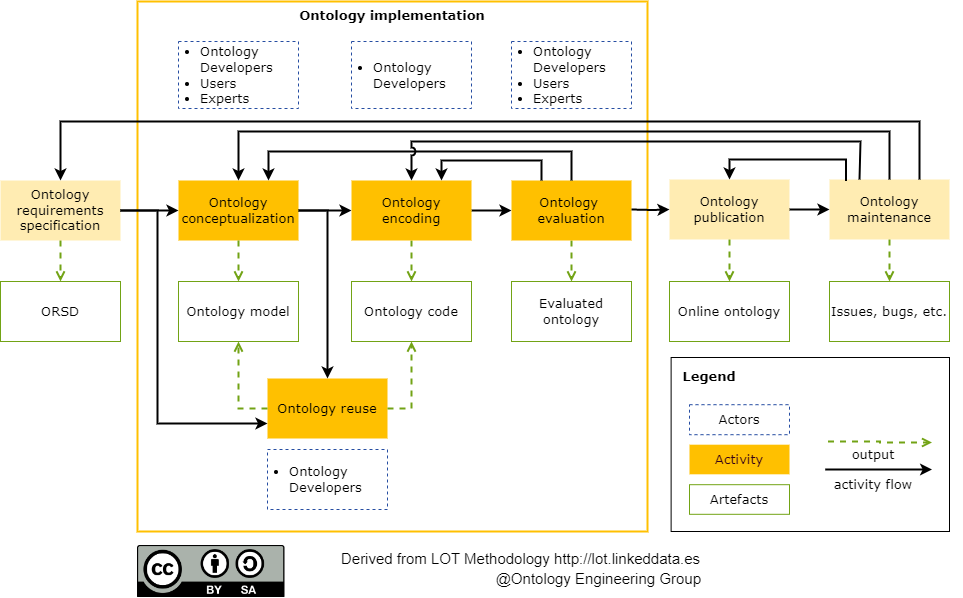
\includegraphics[width=\linewidth]{figures/chapter-3/LOT.png}
    \caption{Ontology development workflow based on the LOT methodology.}
    \label{fig:lot}
\end{figure}

Taking into account the requirements specified in the ontology's ORSD, its first conceptualisation was then generated through a visualisation tool, the Chowlk Visual Notation tool\footnote{The Chowlk Converter tool and respective usage instructions are available at \url{https://chowlk.linkeddata.es/} (accessed on 14 June 2023).}~\citep{chavez-feria_chowlk_2022}, followed by feedback from experts. The generated conceptualisation diagram was then used to generate the first version of the ontology encoding as a Turtle file.
Furthermore, after the generation of the first version of the ontology, the created terms were evaluated against a set of use case scenarios and using SPARQL queries. From this evaluation, if necessary, new concepts were added to the ontology and the ORSD was also updated accordingly. The ontology was also evaluated by using the OntOlogy Pitfall Scanner (OOPS!)\footnote{The OOPS! tool is available at \url{https://oops.linkeddata.es/} (accessed on 14 June 2023).}~\citep{poveda-villalon_oops_2014} to detect common errors in ontology development, such as missing domain or range properties or missing annotations, and using FOOPS!\footnote{The FOOPS! tool is available at \url{https://w3id.org/foops} (accessed on 30 November 2023).}, the Ontology Pitfall Scanner to ensure ontology alignment with the Findable, Accessible, Interoperable and Reusable (FAIR) principles~\citep{garijo_foops_2021}.
As a final evaluation, ontology classes and properties and, in particular, their definitions were reviewed by legal and technical experts and, when applicable, connected with the relevant legal rules, guidelines, and other literature.

The ontologies are published using the \url{w3id.org}, ``Permanent Identifiers for the Web'', service\footnote{This service is run by the W3C Permanent Identifier Community Group (\url{https://www.w3.org/community/perma-id/}, accessed on 22 October 2023).}.
This service provides a secure and permanent re-direction and content negotiation service that serves both human-readable documentation and a machine-readable file from the same URI.
The source code is hosted on GitHub\footnote{\url{https://github.com/} (accessed on 22 October 2023)} and version control is done using Git\footnote{\url{https://git-scm.com/} (accessed on 22 October 2023)}.

% TODO: mention SHACL validation + SPARQL for CQs}

% TODO: publication/preservation of code -- Zenodo, DOI, w3id
\section{Evaluation Methodology}
\label{sec:eval_methodology}

As previously mentioned, the work for this Thesis involves two distinct research fields, law and ontology engineering.
As such, distinct evaluation methods were followed to assess the hypotheses identified in Section~\ref{sec:hypotheses}, in particular:

\begin{enumerate}
    \item [\textbf{E1.}] (for H1.) The goal of this evaluation is to determine the alignment of the developed models to represent consent terms and fine-grained policies for the processing of personal data with the EU's General Data Protection Regulation. To this end, the proposed vocabularies were validated by legal experts through collaboration with members of W3C DPVCG and legal scholars from the PROTECT ITN. Moreover, alignment with the ISO/IEC 27560 standard on consent records and receipts was also verified.
    \item [\textbf{E2.}] (for H2a., H2b., and H2c.) The goal of this evaluation is to assess whether the developed methods can be used to establish access control conditions, describe metadata related to decentralised personal datastores, and represent information related to data subject's rights. To this end, the quality of the proposed ontologies was evaluated by detecting common pitfalls and alignment with FAIR principles, and their ability to answer the competency questions through SPARQL queries was also verified.
    \item [\textbf{E3.}] (for H3.) The goal of this evaluation is to test whether the developed ontologies and policy-based algorithms can be used to define data access agreements that fulfil the data subjects' privacy preferences. To this end, a proof of concept implementation for policy matching towards the generation of data access agreements was built to evaluate the proposed algorithms against a specific real-world use case involving health data sharing. Furthermore, proof of concept prototypes to generate policies and exercise the GDPR's right of access were also built, to assess the applicability of the developed vocabularies in the development of decentralised applications, in addition to a data altruism protocol which verifies the extensibility of the proposed vocabularies to cover other data protection laws, e.g., the EU's Data Governance Act.
\end{enumerate}


\part{GDPR-ALIGNED VOCABULARIES FOR PERSONAL DATASTORES}

\chapter{Vocabularies for Personal Datastores}
\label{chap:vocabularies}

\begin{tcolorbox}[colback=royallavender!40]
The content of this Chapter has already been partially included in the articles published during this Thesis \citep{esteves_odrl_2021,esteves_using_2023,esteves_fostering_2022}.
\end{tcolorbox}

\begin{tcolorbox}[colback=royallavender!10]
The source code produced during the development of this chapter is stored at:
\begin{itemize}
    \item \url{https://w3id.org/oac/repo}
    \item \url{https://w3id.org/oac/policies}
    \item \url{https://w3id.org/plasma/repo}
    \item \url{https://w3id.org/people/besteves/justifications/repo}
\end{itemize}
\end{tcolorbox}
% repo with rights exercising missing

This Chapter builds upon existing Semantic Web standards and specifications to develop a set of vocabularies that can support data subjects in the expression of their privacy preferences when it comes to accessing their data and exercising their rights, as well as data controllers to deal with their \textit{``[t]ransparent information''} requirements, explicitly set in GDPR's Articles 12--14.
As previously established in Section \ref{sec:sota_solid}, Solid's access control and interoperability specifications do not contain the terms to satisfy said requirements, and as such, the incorporation of these vocabularies will lead to a GDPR-aligned personal datastore.

Thus, Section \ref{sec:oac} describes the development of an ODRL profile (OAC) with the main goal of defining legally aligned policies that express permissions and/or prohibitions associated with purpose-based access to data stored in decentralised storage environments, such as Solid Pods.
Such policies will be used to express the data subjects' preferences concerning the access to their \textit{personal} data, to represent requests to access data and to record the agreed access conditions for future inspection.

Section \ref{sec:plasma} describes the development of a metadata language for Solid (PLASMA) to provide consistent taxonomies to describe the entities, infrastructure, policies, notices, registries and logs necessary to understand and establish responsibilities and accountability within the Solid ecosystem.
PLASMA utilises OAC to express data policies, provides a set of conformance conditions that should be met by Pod, app, and service providers, as well as users and agents, to comply with the established specification, and a description of workflows where PLASMA terms should be used to satisfy such conformance conditions.

Section \ref{sec:rights_exercising} showcases the usage of vocabulary-based, e.g. DPV, DCMI, PROV-O and DCAT, patterns to describe rights exercising metadata with the goal of providing uniform records of data subject rights exercising activities.

Section \ref{sec:evaluation} presents the results of the ontologies quality evaluation, including the detection of common pitfalls with OOPS!, alignment with FAIR principles with FOOPS! and validation of competency questions with SPARQL queries.

The methodology followed to develop and evaluate the vocabularies described in this Chapter is described in Section \ref{sec:ontology_engineering}.

\section{Background}
\label{sec:background_vocabs}

As established through the state of the art and in the comparative analysis performed in Sections \ref{sec:sota_vocabularies_analysis} and \ref{sec:sota_policies_analysis}, DPV contains the highest number of concepts to model GDPR's rights and obligations and their privacy terms, is being actively developed and maintained, is open and accessible, and ODRL supports the modelling of deontic concepts, e.g., permissions or obligations, constraints, e.g., spatial and temporal, and types of policies, e.g., offers, requests and agreements, and has a mechanism to develop extensions to its vocabulary through profiles.
As such, they can be used as a starting point to express policies for access to personal data, while invoking privacy and data protection-specific terms.

Figure \ref{fig:odrl} presents a diagram of the ODRL Information Model.
Its main goal is to \textit{``enable flexible Policy expressions by allowing the policy author to include as much, or as little, detail in the Policies''} \citep{iannella_odrl_2018}, using the terms defined in the ODRL Vocabulary \& Expression specification \citep{iannella_odrl_vocab_2018}.
Table \ref{tab:odrl} provides an overview of the concepts modelled in the ODRL vocabulary.

\begin{figure}[htbp]
\caption{ODRL Information Model, adapted from \cite{iannella_odrl_2018}.}
\label{fig:odrl}
\centering
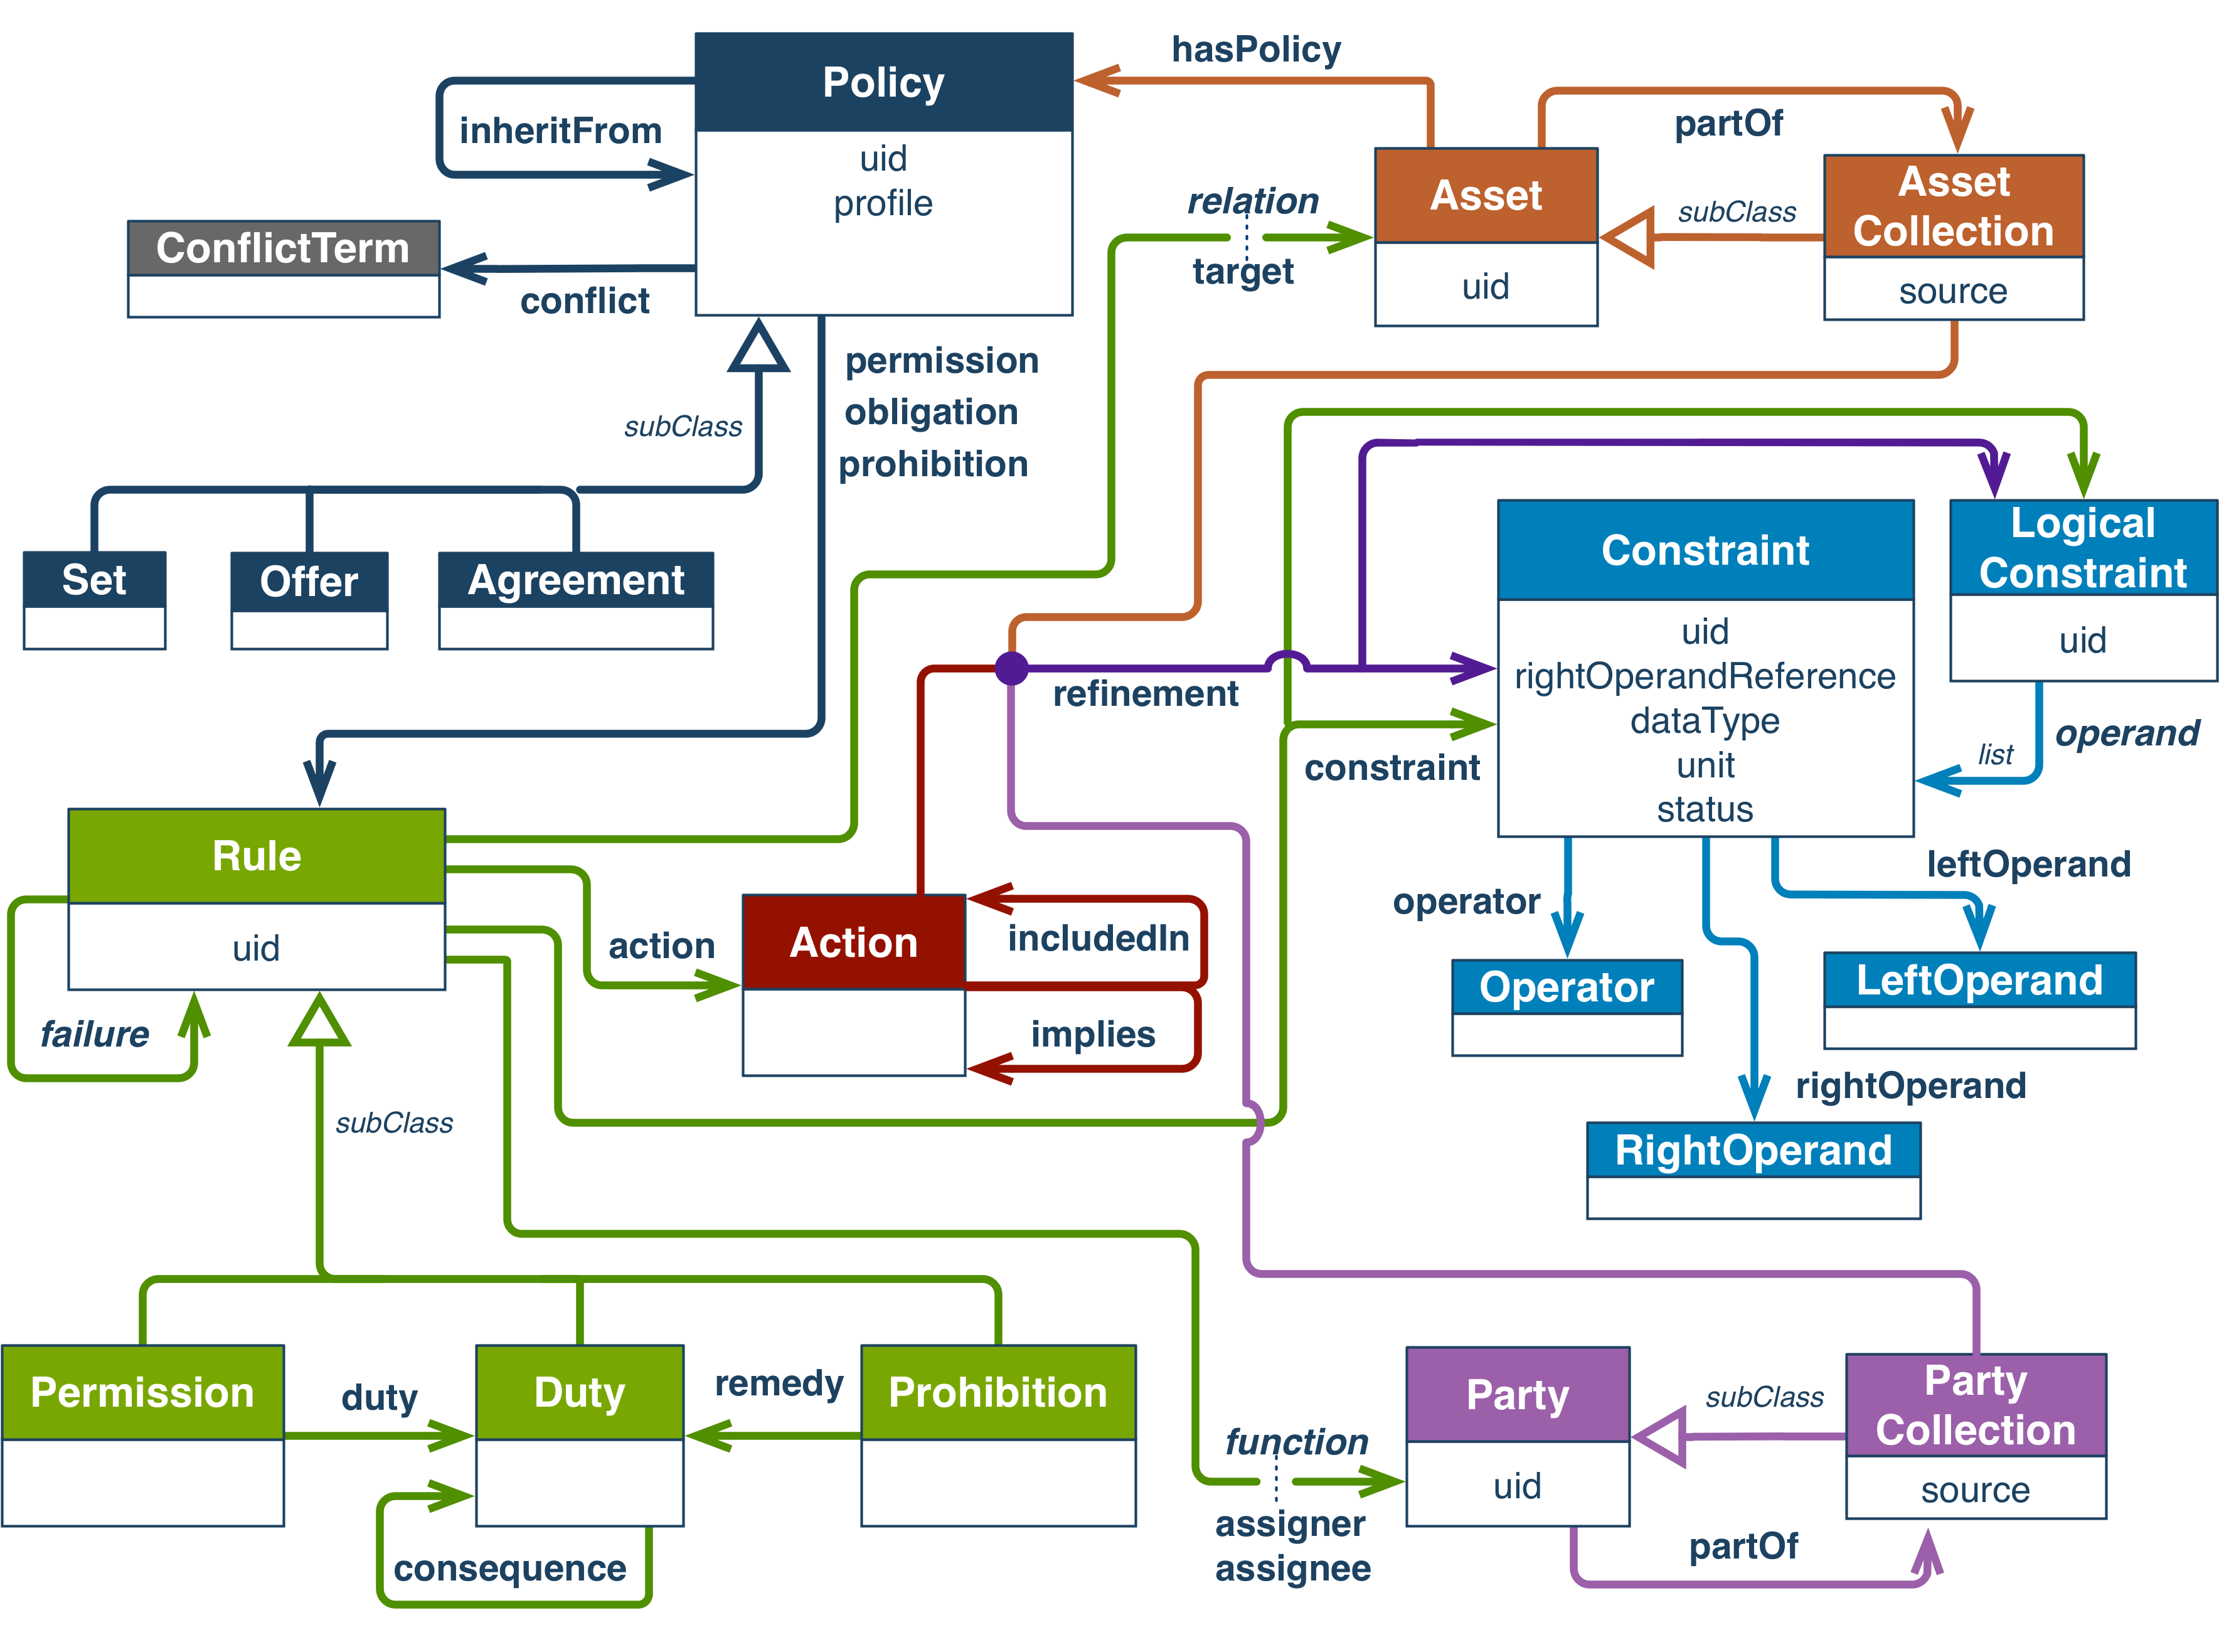
\includegraphics[width=0.8\textwidth]{figures/chapter-4/ODRL.png}
\end{figure}

\begin{table}[htbp]
\caption{Overview of the concepts modelled in the ODRL vocabulary.}
\label{tab:odrl}
\centering
\begin{tabular}{c||c}
Concept & Subclasses \\
\hline\hline
Policy & Agreement, Assertion, Offer, Privacy, Request, Set, Ticket \\
\hline
Rule & Duty, Permission, Prohibition\\
\hline
\begin{tabular}[c]{@{}c@{}}Party\\ functions\end{tabular} & \begin{tabular}[c]{@{}c@{}}assignee, assigner, attributedParty, attributingParty, \\ compensatedParty, compensatingParty, consentedParty, \\ consentingParty, contractedParty, contractingParty, informedParty, \\ informingParty, trackedParty, trackingParty\end{tabular}\\
\hline
Action & \begin{tabular}[c]{@{}c@{}}Attribution, CommericalUse, DerivativeWorks, Distribution, Notice, \\ Reproduction, ShareAlike, Sharing, SourceCode, acceptTracking, \\ aggregate, annotate, anonymize, archive, attribute, compensate, \\ concurrentUse, delete, derive, digitize, display, distribute, \\ ensureExclusivity, execute, extract, give, grantUse, include, index, \\ inform, install, modify, move, nextPolicy, obtainConsent, play, \\ present, print, read, reproduce, reviewPolicy, sell, shareAlike,\\ stream, synchronize, textToSpeech, transfer, transform, translate,\\ uninstall, use, watermark\end{tabular} \\
\hline
Operand & and, andSequence, or, xone \\
\hline
\begin{tabular}[c]{@{}c@{}}Left\\ Operand\end{tabular}    & \begin{tabular}[c]{@{}c@{}}absolutePosition, absoluteSize, absoluteSpatialPosition, \\ absoluteTemporalPosition, count, dateTime, delayPeriod, \\ deliveryChannel, elapsedTime, event, fileFormat, industry, \\ language, media, meteredTime, payAmount, percentage, product, \\ purpose, recipient, relativePosition, relativeSize, relativeSpatialPosition, \\ relativeTemporalPosition, resolution, spatial, spatialCoordinates, \\ systemDevice, timeInterval, unitOfCount, version, virtualLocation\end{tabular}\\
\hline
Operator & \begin{tabular}[c]{@{}c@{}}eq, gt, gteq, hasPart, isA, isAllOf, isAnyOf, isNoneOf, isPartOf,\\ lt, lteq, neq\end{tabular}\\
\hline
\begin{tabular}[c]{@{}c@{}}Right\\ Operand\end{tabular}   & policyUsage
\end{tabular}
\end{table}

The model also expresses which properties are mandatory and optional to define policies and their respective entities, assets, actions and constraints.
Both recommendations are being promoted and maintained by the W3C ODRL CG, which also aims to support the development of ODRL profiles and publish reports related to ODRL usage, such as:

\begin{itemize}
    \item the ODRL Implementation Best Practices \citep{smith_odrl_2023}, which presents examples of ODRL usage and describes good implementation practices;
    \item the ODRL Profile Best Practices \citep{steidl_odrl_2023}, which presents guidelines for the development, definition and publication of ODRL Profiles;
    \item the ODRL Formal Semantics \citep{fornara_odrl_2023}, which discusses and provides a formal semantics specification to ensure the correctness and consistency of services that use ODRL.
\end{itemize}

While ODRL presents itself as a well-tested resource for the expression of policies, it does contain the concepts to model personal data-related access policies or to invoke data protection-related terms.
As such, its profile mechanism provides an opportunity to extend the ODRL vocabulary with these missing terms, e.g., by associating it with personal data-focused vocabularies such as DPV.
Figure \ref{fig:dpv_base} provides an overview of DPV's core concepts.

\begin{figure}[htbp]
\caption{Overview of DPV's core concepts, adapted from \cite{pandit_primer_2022}.}
\label{fig:dpv_base}
\centering
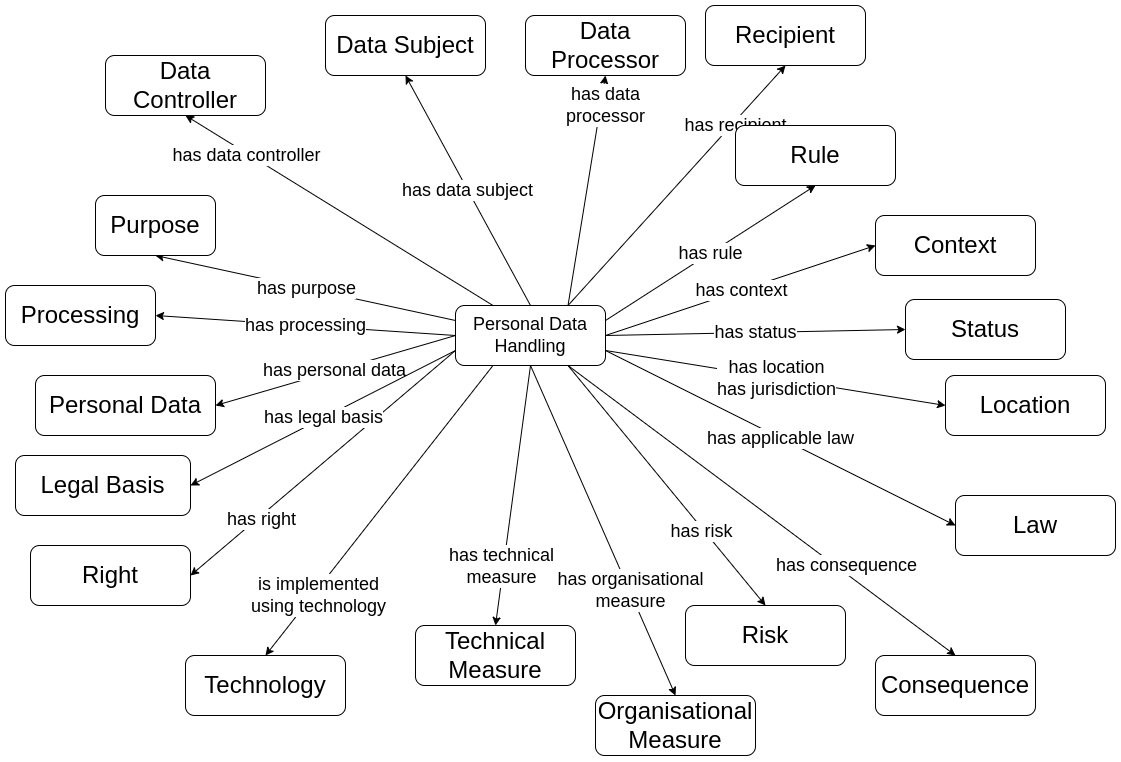
\includegraphics[width=0.8\textwidth]{figures/chapter-4/dpv-base.png}
\end{figure}

As indicated in the state of the art Chapter of this Thesis, DPV provides the most extensive list of data protection-related terms among the evaluated solutions.
Table \ref{tab:dpv_main_contributions} includes a list of the taxonomies defined in DPV's main specification, as well as the number of classes and properties defined in each taxonomy and, in the third column, the number of classes and properties which were contributed to the vocabulary in the course of the development of this Thesis. 

\begin{table}[htbp]
\centering
\caption[Taxonomies defined in DPV's main specification.]{Taxonomies defined in DPV's main specification, with the respective number of defined classes and properties, as well as the number of contributions of this Thesis to the vocabulary.}
\label{tab:dpv_main_contributions} 
\begin{tabular}{ c||c|c}
 Taxonomies & \#Classes (\#Properties)  & Contributions \\
 \hline\hline
 Entities & 4 (7) & 1 (4) \\
 \hline
 Legal Roles & 9 (9) & 0 (0) \\
 \hline
 Authorities & 5 (2) & 0 (0) \\
 \hline
 Organisations & 9 (0) & 0 (0) \\
 \hline
 Data Subjects & 26 (2) & 17 (0) \\
 \hline
 Purposes & 78 (2) & 20 (0) \\
 \hline
 Processing & 45 (1) & 0 (0) \\
 \hline
 Storage Conditions \& Automation & 29 (5) & 3 (0) \\
 \hline
 Scale of Processing & 27 (4) & 0 (0) \\
 \hline
 Data & 16 (2) & 0 (0) \\
 \hline
 TOMs & 139 (6) & 4 (0) \\
 \hline
 Legal Bases & 34 (5) & 0 (0) \\
 \hline
 Duration \& Frequency & 23 (11) & 7 (3) \\
 \hline
 Status & 39 (5) & 0 (0) \\
 \hline
 Location \& Jurisdiction & 25 (5) & 0 (0) \\
 \hline
 Risk \& Impacts & 16 (12) & 4 (3) \\
 \hline
 Rights & 9 (2) & 9 (0) \\
 \hline
 Rules & 4 (4) & 4 (4) \\
\end{tabular}
\end{table}

Moreover, the DPVCG also published a primer document \citep{pandit_primer_2022}, which provides a description of DPV and its concept modelling, examples which illustrate how the provided concepts should be used to represent metadata regarding personal data handling activities and guidelines towards the application of DPV in particular use cases, e.g., consent record keeping or rights exercising.
Additionally, as previously described in \ref{sec:dpv}, the DPVCG developed six extensions to the main specification, to model personal data categories, GDPR-specific concepts, technology and jurisdiction-relevant concepts, risk and EU rights concepts.
Table \ref{tab:dpv_extensions_contributions} includes a list of the DPV's extensions, as well as the number of classes and properties defined in each extension and, in the third column, the number of classes and properties which were contributed to the extensions in the course of the development of this Thesis.

\begin{table}[htbp]
\centering
\caption[DPV's extensions.]{DPV's extensions with the respective number of defined classes and properties, as well as the number of contributions of this Thesis to the extensions.}
\label{tab:dpv_extensions_contributions} 
\begin{tabular}{ c||c|c}
 Extensions & \#Classes (\#Properties)  & Contributions \\
 \hline\hline
 Personal data & 206 (0) & 3 (0) \\
 \hline
 GDPR & 92 (0) & 16 (0) \\
 \hline
 Technology & 60 (8) & 0 (0) \\
 \hline
 Jurisdiction & 452 (0) & 0 (0) \\
 \hline
 Risk & 376 (0) & 0 (0) \\
 \hline
 EU Rights & 62 (0) & 0 (0) \\
\end{tabular}
\end{table}

Additionally, existing work, using ODRL's profile mechanism, has been published to instantiate GDPR Articles as ODRL obligations~\citep{agarwal_legislative_2018} and as permissive, prohibitive or obligated policies with dispensations, which are translated into Answer Set Programming (ASP) rules for compliance checking~\citep{de_vos_odrl_2019}.
Other ODRL-based works have been published, related to (i) the representation of agreements to access data and execute algorithms in digital marketplaces~\citep{shakeri_modeling_2019}, (ii) the dynamic generation of privacy policies for IoT-generated data~\citep{canobenito_injecting_2023}, and (iii) the representation of privacy policies as ODRL requests, which use a small subset of DPV's taxonomies and do not follow the ODRL Information Model~\citep{krasnashchok_towards_2020}.
\section{ODRL profile for Access Control}
\label{sec:oac}

This Section describes the development of OAC, an ODRL profile for Access Control, to express access policies associated with data stored in decentralised datastores.

\subsection{Profile requirements specification}
\label{sec:oac_requirements}

This Section outlines the motivation and identified requirements for the development of the OAC profile.
As previously mentioned, personal datastores, such as Solid Pods, need to deal with GDPR's requirements, particularly the information requirements set out in Articles 13 and 14, such as the identity of the controller, the purpose for processing, the personal data categories being processed, or the legal basis being used, if they are to be adopted as a legally compatible solution for the sharing of personal data in Europe.
Taking Solid as a use case, this information can be given to Solid users by employing conventional methods, such as a notice provided through the data requester's website.
However, for individuals to control their data practices, the Solid Pod must also record this information so that the individual has the opportunity to:

\begin{enumerate}
    \item [(i)] inspect their personal data within an environment under their control;
    \item [(ii)] store it for accountability purposes;
    \item [(iii)] determine their data access preferences; and
    \item [(iv)] be assisted in enforcing said preferences.
\end{enumerate}

To achieve this, it is necessary to understand the provisions of the law regarding the information that needs to be provided, including the particular requirements of certain legal bases such as consent, and the forms of control that individuals want to have or the information they want to know in the context of the handling of their personal data.
Therefore, based on these considerations, the usage of ODRL and DPV is motivated by the following needs: 

\begin{itemize}
  \item[1.]Organisations need to:
    \begin{itemize}
      \item[a)]Specify machine-readable data handling policies, which should be accessible by users;
      \item[b)]Document provenance information related to their personal data processing activities, including notices and activity logs;
      \item[c)]Determine and fulfil applicable rights and obligations based on specific data protection laws or other contextual information, e.g., specific categories of personal data;
      \item[d)]Implement security measures by default and by design, specifically related to personal data access.
    \end{itemize}

    \item[2.]Users need to:
    \begin{itemize}
      \item[a)]Express human-centric data-sharing preferences, e.g., willingness to share a specific data type for non-profit research or to prohibit processing for profiling purposes;
      \item[b)]Specify broad permissions, e.g., allow data access for scientific research, or restrict third party data collection;
      \item[c)]Specify narrow permissions, e.g., allow access to phone contact details for a particular app, or deny access to a specific resource;
      \item[d)]Have a policy conflict strategy, e.g., generally deny access to location data, but include an exception for specific applications;
      \item[e)]Understand who is using which data categories, for what purposes, sharing it with whom, and under what legal basis.
    \end{itemize}
    
\end{itemize}

Moreover, taking into consideration the previously described motivation points, the following requirements can then be specified for the OAC profile:

\begin{itemize}
      \item[R1.]Support specifying user preferences as policies.
      \item[R2.]Incorporate vocabulary specifying or aligned to legal concepts.
      \item[R3.]Support specifying permissions and prohibitions at arbitrary granularity.
      \item[R4.]Support identifying and resolving conflicts based on scope.
      \item[R5.]Record policies used to authorise access to data.
      \item[R6.]Support querying policies and authorisations for introspection of data access.
\end{itemize}

As such, following the LOT methodology, these requirements are consolidated in the profile's ORSD available in Table \ref{tab:OAC_ORSD}.
As Solid's current access control mechanisms only partially implement R1, R3, and R5, OAC allows its users to declare not only granular permissive policies but also prohibitive policies, both aligned with legal requirements, which can be stored in their decentralised datastores for future inspection and can be used with additional constraints and contextual information.

\begin{table}[htbp]
\centering
\caption{Ontology Requirement Specification Document of the OAC profile.}
\label{tab:OAC_ORSD}
\scriptsize
\begin{tabular}{| l | l | l | l  | l | l | l |l| }
\hline
\multicolumn{8}{|c|}{\cellcolor[HTML]{A0A0A0}\textbf{ODRL Profile for Access Control}} \\ \hline
\multicolumn{8}{|c|}{\cellcolor[HTML]{EFEFEF}\textbf{1. Purpose}} \\ \hline
\multicolumn{8}{| p{12.0cm} |}{The purpose of this profile of ODRL is to support policies determining the access to personal data stored in decentralised storage environments, such as Solid Pods.} \\ \hline
\multicolumn{8}{|c|}{\cellcolor[HTML]{EFEFEF}\textbf{2. Scope}} \\ \hline
\multicolumn{8}{| p{12.0cm} |}{The scope of this profile is limited to the definition of an ODRL Profile for Access Control in decentralised settings. In particular, the introduced elements will serve one of these purposes: (i) define actions supporting the enforcement of current ACL verbs, (ii) define data protection-related actions and restrictions defined in GDPR, (iii) any vocabulary element to support policy patterns that can be anticipated to be common, and (iv) elements necessary to support the authorisation reasoning decision. } \\ \hline
\multicolumn{8}{|c|}{\cellcolor[HTML]{EFEFEF}\textbf{3. Implementation Language}} \\ \hline
\multicolumn{8}{| p{12.0cm} |}{RDF, RDFS} \\ \hline
\multicolumn{8}{|c|}{\cellcolor[HTML]{EFEFEF}\textbf{4. Intended End-Users}} \\ \hline
\multicolumn{8}{| p{12.0cm} |}{Developers of decentralised storage servers and applications, such as Solid servers and apps.} \\ \hline
\multicolumn{8}{|c|}{\cellcolor[HTML]{EFEFEF}\textbf{5. Intended Uses}} \\ \hline
\multicolumn{8}{| p{12.0cm} |}{
Use 1. Declaration of a policy by an individual storing personal data in a decentralised datastore, such as a Solid Pod. \newline 
Use 2. Request of data made by an entity, service or application to gain access to the data in different modalities. \newline
Use 3. Records of data access with transparent information related to the policy matching algorithm, including contextual information. 
 } \\ \hline
\multicolumn{8}{|c|}{\cellcolor[HTML]{EFEFEF}\textbf{6. Ontology Requirements}} \\ \hline
\multicolumn{8}{|c|}{\cellcolor[HTML]{EFEFEF}\textbf{a. Non-Functional Requirements}}    \\ \hline
\multicolumn{8}{| p{12.0cm} |}{
NFR 1. The profile is published online with HTML documentation, following W3C's specification format. } \\ \hline
\multicolumn{8}{|c|}{\cellcolor[HTML]{EFEFEF}\textbf{b. Functional  Requirements: Groups of Competency Questions}}  \\ \hline
\multicolumn{5}{|c|}{\cellcolor[HTML]{EFEFEF}CQG1. Related to access} & \multicolumn{3}{|c|}{\cellcolor[HTML]{EFEFEF}CQG2. Related to GDPR} \\ \hline %\multicolumn{4}{c|}{\cellcolor[HTML]{EFEFEF}}    \\ \hline
\multicolumn{5}{ | m{7cm} |}{
CQ1. Which policy type is being defined? \newline
CQ2. Which actions are defined in the policy? \newline
CQ3. Which data types are mentioned in the policy? \newline 
CQ4. Which policy constraints need to be fulfilled? \newline 
CQ5. Who are the parties intervening in the policy? \newline 
CQ6. Which is the conflict strategy of a policy? \newline 
CQ7. What are the contextual elements that need to be considered in the policy matching algorithm? } & 
\multicolumn{3}{ m{5cm} |}{
CQ8. Which information about personal data and its processing is necessary to have legally aligned policies? \newline 
CQ9. What identification information needs to be provided by the policy parties? \newline 
}\\ \hline
\end{tabular}
\vspace{-0.1in}
\end{table}

%For continued interoperability and adherence to the specification, the proposed extension to Solid’s ACL must ideally continue to implement existing functionality while incorporating the legal and user-centric requirements.

Lastly, it should be clear that OAC is \textbf{not dependent on Solid}, as it is not based on any Solid-specific vocabularies, and can be used in other decentralised data environments.
Nevertheless, throughout this Thesis, the use of OAC is demonstrated through the Solid ecosystem as it is an example of the implementation of a decentralised environment for the sharing of (personal) data that is based on the Semantic Web stack of technologies.

\subsection{Profile implementation}
\label{sec:oac_implementation}

This ODRL profile relies on DPV, for the invocation of legal concepts related to data protection and privacy, and ACL, for the expression of access mode operations, to specify complex permissions, prohibitions or duties over the access to personal data resources.

Moreover, OAC policies can be used to add a new layer to decentralised data systems -- a layer that is currently missing from the Solid ecosystem for instance -- that will come between the data and the access authorisation, e.g., ACL or ACP authorisations, layers in order to provide a richer access control mechanism to such systems.
As an access control mechanism's main goal is to determine access by users or software agents to digital resources, the entities generating and/or providing the data must able to express policies that satisfy their preferences, while users or software agents who wish to access said data must be able to define policies that describe their data handling activities. 
By using these policies in an algorithm to match incoming access requests for data, an agreement over the access to a certain resource or type of data can be defined and the decentralised data system can provide a fine-grained access control mechanism to its users.
As such, OAC reuses ODRL's \texttt{Offer} policies to express the conditions for access to personal data stored in decentralised data systems, e.g. Solid Pods, \texttt{Request} policies to express users or software agents' access requests and \texttt{Agreement} policies to describe the agreed conditions for access to the data. 
The three types of policies are defined below, according to their definition provided in the ODRL Vocabulary \& Expression 2.2 Recommendation specification \citep{iannella_odrl_vocab_2018}:

\begin{itemize}
    \item \textbf{Offer} -- Policy that proposes the assigner's rules over an asset and does not grant any privileges to assignees.
    \item \textbf{Request} -- Policy that proposes the assignee's rules over an asset and does not grant any privileges to any parties.
    \item \textbf{Agreement} -- Policy issued by an assigned that grants privileges to the assignee over an asset.
\end{itemize}

OAC's core concepts are illustrated in Figure~\ref{fig:oac_diagram} and Tables \ref{tab:profile_classes} and \ref{tab:profile_properties} specify the alignment between the ODRL, DPV, and ACL terms to ensure that their semantics are correctly interpreted by OAC implementers.

%Its core concepts are the Preference and Requirement policies, a new set of operators to constraint the defined Purposes, Recipients, Legal Basis, Technical and Organisational Measures, Technology and Identity Provider constraints (which will require the usage of DPV's taxonomies), new properties to specify policies for applications and services, Processing and Access actions, as well as Personal Data Categories, and Legal Entities.

\begin{figure}[htbp]
    \centering
    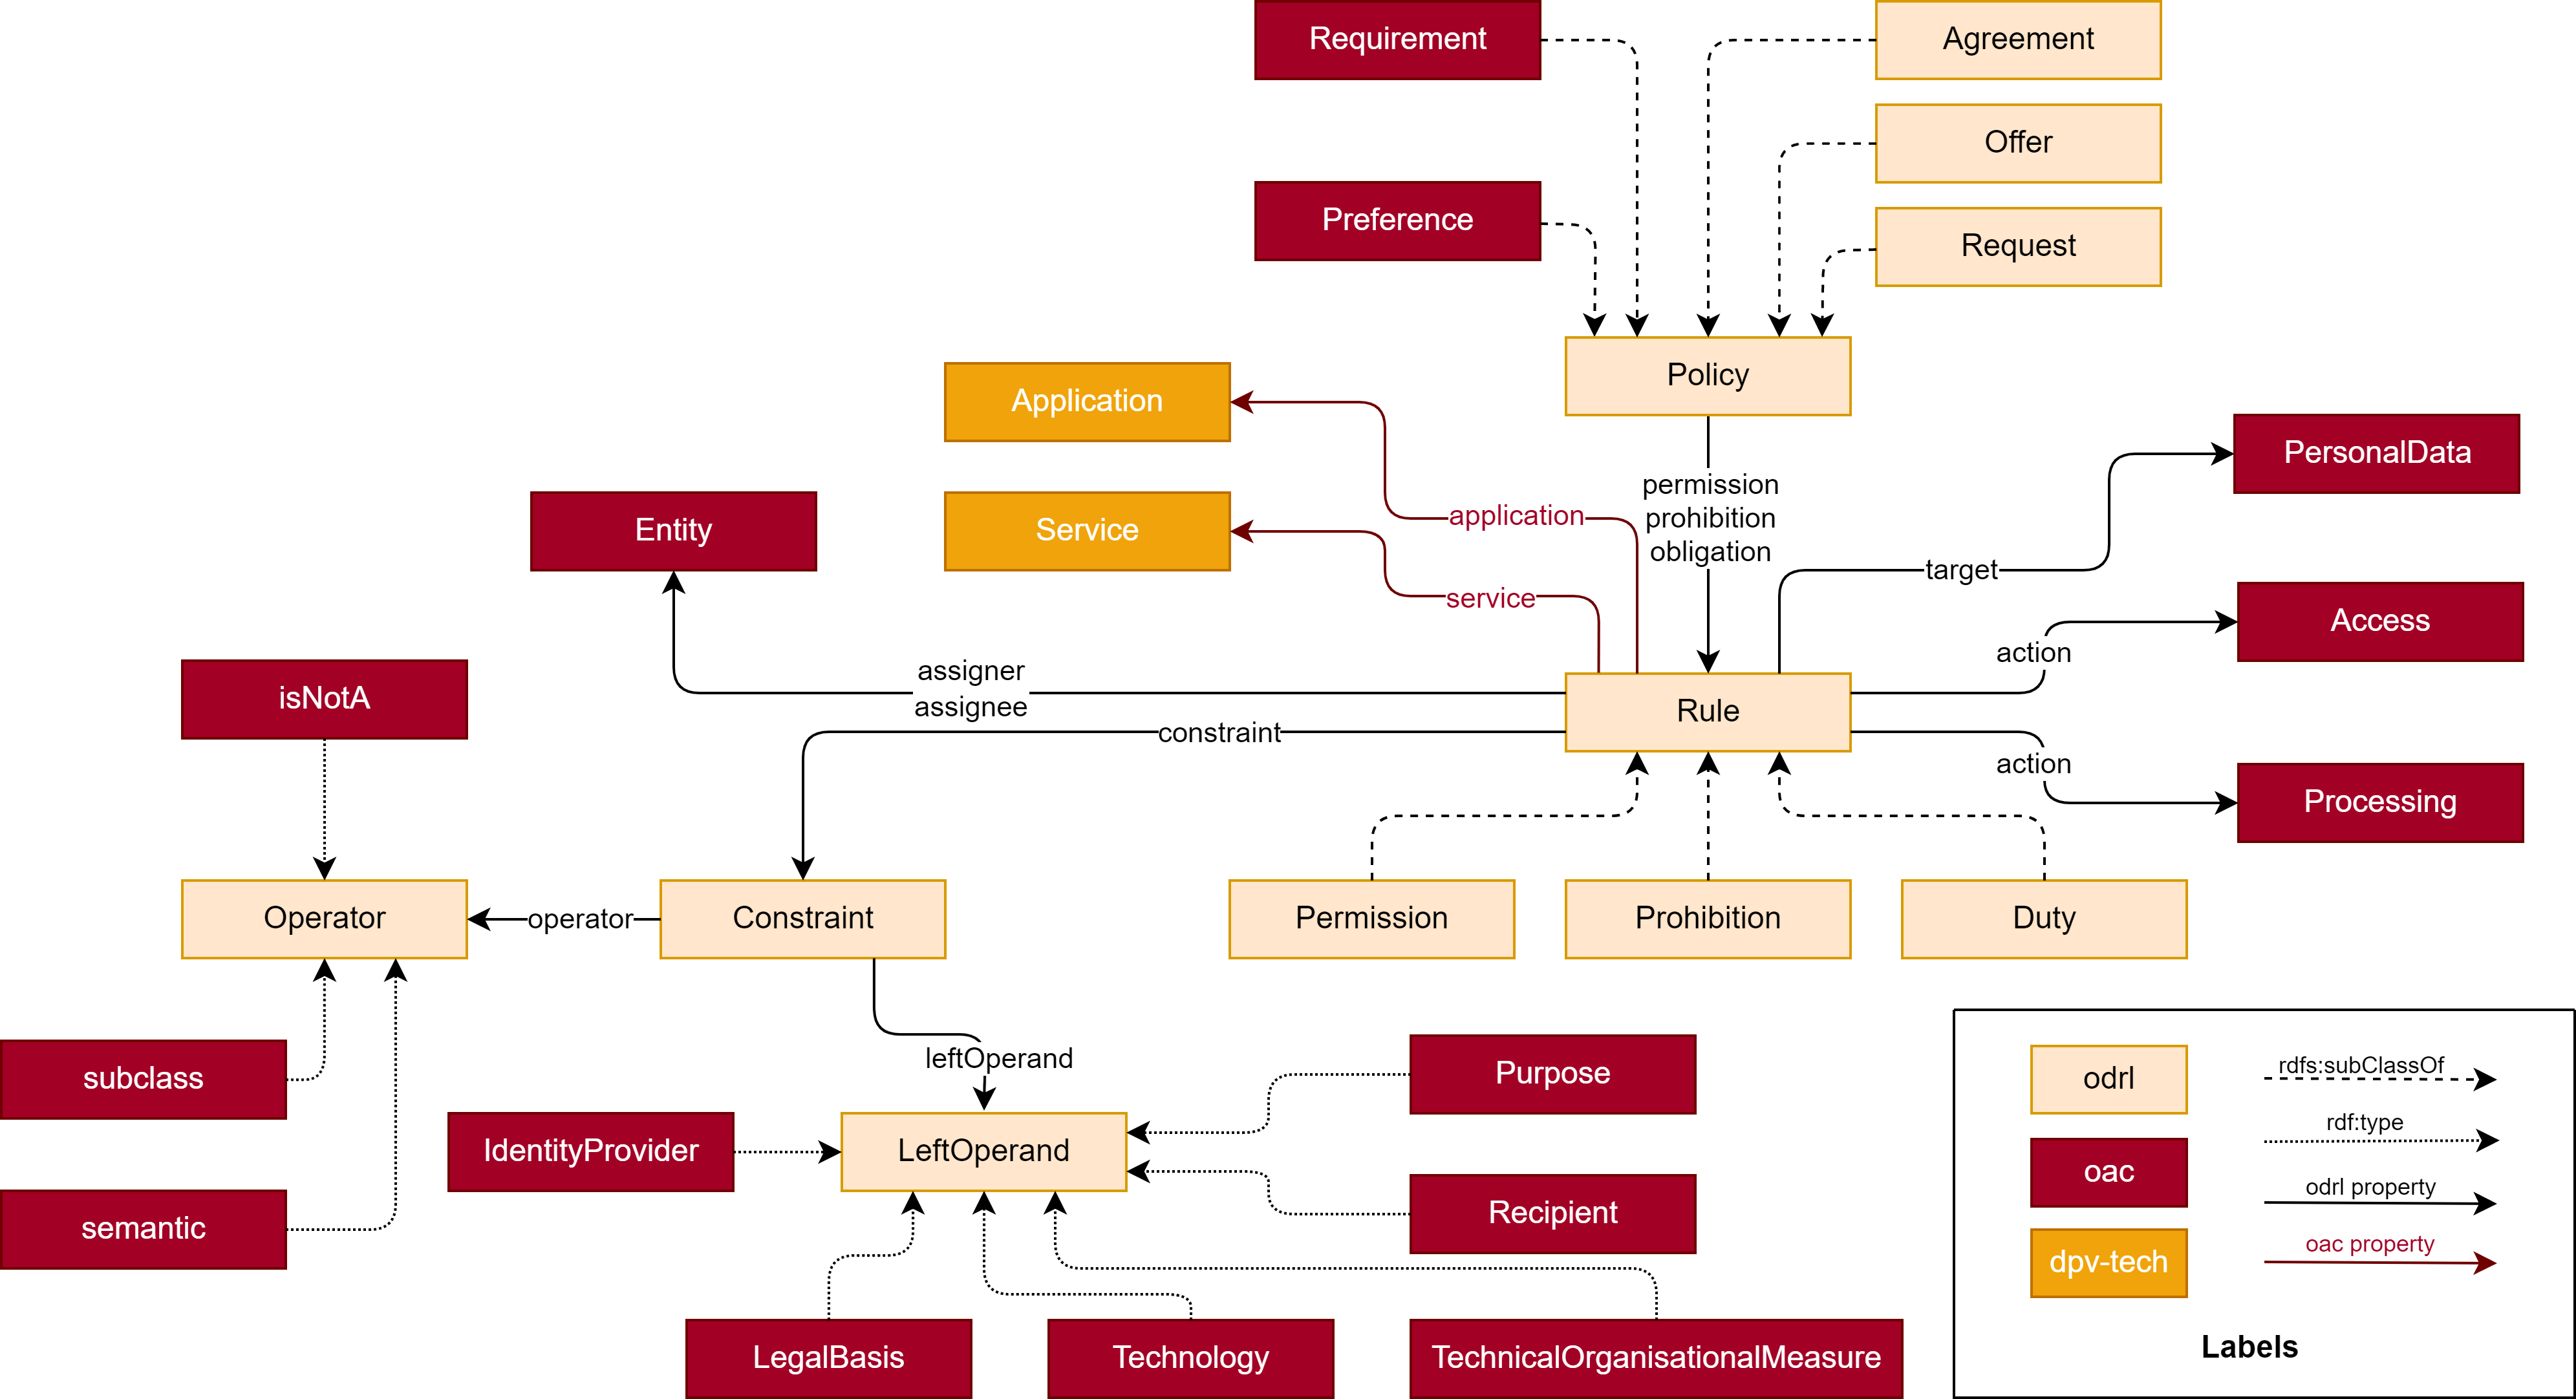
\includegraphics[width=\linewidth]{figures/chapter-4/oac_diagram.png}
    \caption{Diagrams of the concepts specified by the OAC profile.}
    \label{fig:oac_diagram}
\end{figure}

Two new types of policies, which can be combined in ODRL offers, are specified to deal with the preferences and requirements of users who wish to define rules for the processing of their personal data:

\begin{itemize}
    \item \textbf{Preference} -- Soft policy that expresses the assigner's preferences over a personal data asset which may not be satisfied and must not grant any privileges to assignees. If a preference policy set by party A does not match a request policy from party B, the request can still be accepted if party A accepts party B's request conditions.
    \item \textbf{Requirement} -- Hard policy that expresses the assigner's preferences over a personal data asset which must be satisfied and must not grant any privileges to assignees. If a requirement policy set by party A does not match a request policy from party B, the request must be denied even if party A accepts party B's request conditions.
\end{itemize}

\begin{table}[htbp]
\centering
\caption{Classes and named individuals specified in the OAC profile.}
\label{tab:profile_classes}
\resizebox{\textwidth}{!}{
\begin{tabular}{c||c|c}
Profile term & Instance of & Subclass of \\
\hline\hline
\texttt{oac:Preference} & & \texttt{odrl:Policy} \\
\hline
\texttt{oac:Requirement} & & \texttt{odrl:Policy} \\
\hline
\texttt{oac:isNotA} & \texttt{odrl:Operator} & \\
\hline
\texttt{oac:subclass} & \texttt{odrl:Operator} & \\
\hline
\texttt{oac:semantic} & \texttt{odrl:Operator} & \\
\hline
\texttt{oac:PersonalData} & \texttt{odrl:Asset} & \texttt{dpv:PersonalData} \\
\hline
\texttt{oac:Access} & \texttt{odrl:Action} & \texttt{acl:Access} \\
\hline
\texttt{oac:Processing} & \texttt{odrl:Action} & \texttt{dpv:Processing} \\
\hline
\texttt{oac:Entity} & \texttt{odrl:Party} & \texttt{dpv:Entity} \\
\hline
\texttt{oac:Purpose} & \texttt{odrl:LeftOperand} & \texttt{dpv:Purpose} \\
\hline
\texttt{oac:Recipient} & \texttt{odrl:LeftOperand} & \texttt{dpv:Recipient} \\
\hline
\texttt{oac:LegalBasis} & \texttt{odrl:LeftOperand} & \texttt{dpv:LegalBasis} \\
\hline
\texttt{oac:TechnicalOrganisationalMeasure} & \texttt{odrl:LeftOperand} & \texttt{dpv:TechnicalOrganisationalMeasure} \\
\hline
\texttt{oac:Technology} & \texttt{odrl:LeftOperand} & \texttt{dpv:Technology} \\
\hline
\texttt{oac:IdentityProvider} & \texttt{odrl:LeftOperand} & \\
\end{tabular}}
\end{table}

\begin{table}[htbp]
\centering
\caption{Properties specified in the OAC profile.}
\label{tab:profile_properties}
\begin{tabular}{c||c|c}
Profile property & Domain & Range \\
\hline\hline
\texttt{oac:service} & \texttt{odrl:Rule}, \texttt{odrl:Policy} & \texttt{dpv-tech:Service} \\
\hline
\texttt{oac:application} & \texttt{odrl:Rule}, \texttt{odrl:Policy} & \texttt{dpv-tech:Application} \\
\end{tabular}
\end{table}

Listing~\ref{list:oac_req_pref} presents an example of an OAC requirement and an OAC preference policies and Listing~\ref{list:oac_offer} an ODRL offer, based on the previously listed requirement and preference policies, as is indicated by the \texttt{dcterms:source} property.
The permission associated with the requirement policy contains the property \texttt{dpv:hasContext} associated with the term \texttt{dpv:Required} to indicate that said permission is a requirement, while the term \texttt{dpv:Optional} is used to identify the rules related with a preference policy.

\begin{listing}[htp]
\caption{OAC requirement and preference policies issued by \url{https://solidweb.me/besteves4/profile/card\#me}.}
\label{list:oac_req_pref}
\begin{minted}{turtle}
<https://solidweb.me/besteves4/policies/requirement1> a oac:Requirement ;
    odrl:uid <https://solidweb.me/besteves4/policies/requirement1> ;
    odrl:profile oac: ;
    dcterms:description "Requirement to read identifier data for identity verification purposes." ;
    dcterms:creator <https://solidweb.me/besteves4/profile/card#me> ;
    dcterms:issued "2023-10-20T18:22:15"^^xsd:dateTime ;
    odrl:permission [
        odrl:assigner <https://solidweb.me/besteves4/profile/card#me> ;
        odrl:target oac:Identifier ;
        odrl:action oac:Read ;
        odrl:constraint <#Constraint_Purpose_IdentityVerification> .

<#Constraint_Purpose_IdentityVerification> a odrl:Constraint ;
    dcterms:title "Purpose for access is to verify the identity of the assigner." ;
    odrl:leftOperand oac:Purpose ;
    odrl:operator odrl:isA ;
    odrl:rightOperand dpv:IdentityVerification .

<https://solidweb.me/besteves4/policies/preference1> a oac:Preference ;
    odrl:uid <https://solidweb.me/besteves4/policies/preference1> ;
    odrl:profile oac: ;
    dcterms:description "Preference to read age data if purpose is not commercial research." ;
    dcterms:creator <https://solidweb.me/besteves4/profile/card#me> ;
    dcterms:issued "2023-10-20T18:26:09"^^xsd:dateTime ;
    odrl:permission [
        odrl:assigner <https://solidweb.me/besteves4/profile/card#me> ;
        odrl:target oac:Age ;
        odrl:action oac:Read ;
        odrl:constraint <#Constraint_Purpose_not_CommercialResearch> .

<#Constraint_Purpose_not_CommercialResearch> a odrl:Constraint ;
    dcterms:title "Purpose for access is not commercial research." ;
    odrl:leftOperand oac:Purpose ;
    odrl:operator oac:isNotA ;
    odrl:rightOperand dpv:CommercialResearch .
\end{minted}
\end{listing}

\begin{listing}[htp]
\caption{ODRL offer issued by \url{https://solidweb.me/besteves4/profile/card\#me}.}
\label{list:oac_offer}
\begin{minted}{turtle}
<https://solidweb.me/besteves4/policies/offer1> a odrl:Offer ;
    odrl:uid <https://solidweb.me/besteves4/policies/offer1> ;
    odrl:profile oac: ;
    dcterms:description "Offer to read identifier data for identity verification and age data if purpose is not commercial research." ;
    dcterms:creator <https://solidweb.me/besteves4/profile/card#me> ;
    dcterms:source <https://solidweb.me/besteves4/policies/requirement1>, <https://solidweb.me/besteves4/policies/preference1> ;
    dcterms:issued "2023-10-20T22:15:34"^^xsd:dateTime ;
    odrl:permission [
        dpv:hasContext dpv:Required ;
        odrl:assigner <https://solidweb.me/besteves4/profile/card#me> ;
        odrl:action oac:Read ;
        odrl:target oac:Identifier ;
        odrl:constraint <#Constraint_Purpose_IdentityVerification>
    ] ;
    odrl:permission [
        dpv:hasContext dpv:Optional ;
        odrl:assigner <https://solidweb.me/besteves4/profile/card#me> ;
        odrl:action oac:Read ;
        odrl:target oac:Age ;
        odrl:constraint <#Constraint_Purpose_not_CommercialResearch>
    ] .

<#Constraint_Purpose_IdentityVerification> a odrl:Constraint ;
    dcterms:title "Purpose for access is to verify the identity of the assigner." ;
    odrl:leftOperand oac:Purpose ;
    odrl:operator odrl:isA ;
    odrl:rightOperand dpv:IdentityVerification .

<#Constraint_Purpose_not_CommercialResearch> a odrl:Constraint ;
    dcterms:title "Purpose for access is not commercial research." ;
    odrl:leftOperand oac:Purpose ;
    odrl:operator oac:isNotA ;
    odrl:rightOperand dpv:CommercialResearch .
\end{minted}
\end{listing}

Additionally, a set of three new ODRL operators, which are currently missing from the ODRL Core vocabulary Recommendation, and two new properties to specify policies applicable to certain services or applications, \texttt{oac:service} and \texttt{oac:application}, which are important stakeholders in decentralised data systems, are specified in OAC.
The newly introduced \texttt{oac:isNotA} operator is used in the \texttt{<\#Constraint\_Purpose\_not\_CommercialResearch>} constraint, in Listing~\ref{list:oac_req_pref}, to indicate that the purpose for access can not be an instance of the right operand of the constraint, e.g., \texttt{dpv:CommercialResearch}.
The \texttt{oac:subclass} operator can be used to indicate that a given left operand is a subclass of the right operand of the constraint, e.g., the purpose constraint of a rule can be a subclass of DPV's research and development purpose such as academic research, non-commercial research or commercial research, and the \texttt{oac:semantic} operator to express that a given left operand is equal to, an instance or a subclass of the right operand of the constraint, e.g., the purpose constraint of a rule can be research and development, an instance of research and development or one of its subclasses such as academic research, non-commercial research or commercial research.

Personal data is defined as an ODRL asset to define personal data-specific access policies, access modes and processing operations are defined as ODRL actions to define policies for specific access modes and/or processing operations which are not covered by ACL's access modes, e.g., \texttt{dpv:Transfer} or \texttt{dpv:Copy}, and DPV's \texttt{Entity} concept is defined as an ODRL party to define entity-specific access policies.
Additionally, when defining ODRL requests, the data requesters might use processing concepts, \texttt{dpv:Use, dpv:Collect, dpv:Share}, as the permitted/prohibited action of the rule that differ from the existing ACL's access modes, \texttt{acl:Read, acl:Write, acl:Append}.
As such, a mapping of ACL verbs to DPV processing operations is provided in OAC for such cases where offers and requests need to be matched and include both ACL access modes and DPV processing operations.
In this mapping, the \texttt{acl:Read} access mode corresponds to \texttt{dpv:Use, dpv:Collect} processing operations, and \texttt{acl:Write} resembles \texttt{dpv:Store, dpv:MakeAvailable}.
Furthermore, as previously mentioned, there are operations such as \texttt{dpv:Share} or \texttt{dpv:Transfer} that do not have a specific corresponding concept in WAC's ACL vocabulary, which require a greater introspection in the integration of legal processing concepts with access control operations.
Moreover, purposes, recipients, legal bases, technical and organisational measures, technologies and identity providers are defined as ODRL constraints to define constraint-restricted access policies.

Listing~\ref{list:oac_request} presents an example of an ODRL request that uses OAC terms and Listing~\ref{list:oac_agreement} an ODRL agreement which is the result of the matching between the offer defined in Listing~\ref{list:oac_offer} and the previously mentioned request.
In this example, Beatriz, identified by \url{https://solidweb.me/besteves4/profile/card#me}, and Arya, identified by \url{https://solidweb.me/arya/profile/card#me}, reach an agreement to allow read access operations over Beatriz's age data for the purpose of academic research in project X.
This \texttt{odrl:Agreement} is the result of the matching of \url{https://solidweb.me/besteves4/policies/offer1} and \url{https://solidweb.me/arya/requests/age_academicResearch}, as indicated by the \texttt{dcterms:references} property.
The legal basis of the agreement is consent, as is specified in the policy with the \texttt{dpv:hasLegalBasis dpv:Consent} terms, and Beatriz and Arya are registered as the data subject and data controller in question, respectively, using the \texttt{dpv:hasDataSubject} and \texttt{dpv:hasDataController} terms.
\beatriz{Policy matching and agreement generation is discussed in Chapter XX.}

\begin{listing}[ht]
\caption{ODRL request issued by \url{https://solidweb.me/arya/profile/card\#me}.}
\label{list:oac_request}
\begin{minted}{turtle}
<https://solidweb.me/arya/requests/age_academicResearch> a odrl:Request ;
    odrl:uid <https://solidweb.me/arya/requests/age_academicResearch> ;
    odrl:profile oac: ;
    dcterms:description "Request to read age data for academic research." ;
    dcterms:creator <https://solidweb.me/arya/profile/card#me> ;
    dcterms:issued "2023-10-21T13:47:56"^^xsd:dateTime ;
    odrl:permission [
        odrl:assignee <https://solidweb.me/arya/profile/card#me> ;
        odrl:action oac:Use ;
        odrl:target oac:Age ;
        odrl:constraint <#Constraint_Purpose_AcademicResearch>
    ] .

<#Constraint_Purpose_AcademicResearch> a odrl:Constraint ;
    dcterms:title "Purpose for access is to conduct academic research in project X." ;
    odrl:leftOperand oac:Purpose ;
    odrl:operator odrl:eq ;
    odrl:rightOperand ex:AcademicResearchProjectX .

ex:AcademicResearchProjectX a dpv:Purpose ;
    rdfs:subClassOf dpv:AcademicResearch ;
    rdfs:label "Conduct research in the academic project X." .
\end{minted}
\end{listing}

\begin{listing}[ht]
\caption{ODRL agreement to read age data for academic research based on consent.}
\label{list:oac_agreement}
\begin{minted}{turtle}
<https://solidweb.me/besteves4/policies/agreement1> a odrl:Agreement ;
    odrl:uid <https://solidweb.me/besteves4/policies/agreement1> ;
    odrl:profile oac: ;
    dcterms:description "Agreement to read age data for academic research based on consent." ;
    dcterms:creator <https://solidweb.me/besteves4/profile/card#me> ;
    dcterms:issued "2023-10-21T13:58:37"^^xsd:dateTime ;
    dcterms:references <https://solidweb.me/besteves4/policies/offer1>, <https://solidweb.me/arya/requests/age_academicResearch> ;
    dpv:hasDataSubject <https://solidweb.me/besteves4/profile/card#me> ;
    dpv:hasDataController <https://solidweb.me/arya/profile/card#me> ;
    dpv:hasLegalBasis dpv:Consent ;
    odrl:permission [
        odrl:assigner <https://solidweb.me/besteves4/profile/card#me> ;
        odrl:assignee <https://solidweb.me/arya/profile/card#me> ;
        odrl:action oac:Read ;
        odrl:target oac:Age ;
        odrl:constraint <#Constraint_Purpose_AcademicResearch>
    ] .
\end{minted}
\end{listing}

This Thesis focuses on \textit{Purpose, Personal Data, Processing, Recipients, Legal Bases, Technical and Organisational Measures} and \textit{Technologies} as the minimum `core concepts' for the OAC profile, and leaves out other DPV concepts such as rights or risks, which can be added at a later stage if needed.
Furthermore, similarly to WAC and ACP, OAC policies can also be defined for particular resources identified by URIs -- in such cases when an access request for a particular data type comes in, the authorisation mechanism must have information about what type of data those particular resources contain or else they will not be returned if they match the data type of the request.
Such information can be stored in a data registry, stored in a e.g. Solid Pod, where resources can be associated with the type of data they contain by using DPV's \texttt{hasPersonalData} property and DPV-PD's taxonomy of personal data categories, e.g., \texttt{<https://solidweb.me/besteves4/private/health/file1> dpv:hasPersonalData dpv-pd:HealthHistory .}

Ultimately, since these policies are stored in the personal datastore for purposes of accountability and transparency, apps and services, based on the stored preferences, requests, and agreements, can be built, e.g., using SPARQL queries, to inquire who is using what data and for what purposes.
Listing~\ref{list:sparql_agreement} presents a SPARQL query to retrieve permitted data accesses by user, data, and purpose from ODRL agreements stored in a decentralised datastore.

\begin{listing}[ht]
\caption{SPARQL query to retrieve authorised data accesses by user, data, and purpose.}
\label{list:sparql_agreement}
\begin{minted}{sparql}
SELECT DISTINCT ?User ?Data ?Purpose WHERE {
    ?a a odrl:Agreement .
    ?a odrl:permission ?perm .
    ?perm odrl:assignee ?User .
    ?perm odrl:target ?Data .
    ?perm odrl:constraint ?c .
    ?c odrl:leftOperand oac:Purpose .
    ?c odrl:operator odrl:eq .
    ?c odrl:rightOperand ?Purpose .
}
\end{minted}
\end{listing}

\subsection{Profile publication and maintenance}
\label{sec:oac_publication}

The ontology human-readable documentation and machine-readable file are available at \url{https://w3id.org/oac} using content negotiation.
The HTML documentation includes a description of the classes and properties of the ontology, that was done in collaboration with domain experts, a diagram with the graphical representation of the ontology, examples of policies defined with the OAC profile, and information related to the policy matching algorithm.
The ontology documentation also includes metadata, such as the identity of the creators and publishers of the ontology, the dates of creation and last modification, or the version number.

The source code is hosted at \url{https://w3id.org/oac/repo}, under the CC-BY-4.0 license.
The repository can also be used by OAC users to suggest new inclusions to the ontology and to report bugs through GitHub Issues.
In addition, the repository at \url{https://w3id.org/oac/policies} contains a growing collection of OAC policies that can be reused by OAC users.
\section{Metadata language for Solid}
\label{sec:plasma}

This Section describes the development of PLASMA, a metadata language for policy-based access control in Solid, to express metadata related to the entities, registries, logs, policies and infrastructure necessary to provide transparency to Solid's data handling practices.

\subsection{PLASMA requirements specification}
\label{sec:plasma_requirements}

This Section outlines the motivation and identified requirements for the development of PLASMA, a Policy LAnguage for Solid’s Metadata-based Access control.
As previously mentioned, Solid builds upon Web's ethical principles\footnote{\url{https://www.w3.org/TR/ethical-web-principles/} (accessed on 22 October 2023)} and standards such as LDP or RDF and, in accordance with its Protocol, relies on said standards to \textit{``realise a space where individuals can maintain their autonomy, control their data and privacy, and choose applications and services to fulfil their needs''} \citep{capadisli_solid_2022}.

Although it was designed with these goals in mind, Solid currently lacks compatibility with data protection regulatory efforts \citep{pandit_making_2023}, such as the GDPR.
In particular, Solid lacks a practical mechanism to enforce GDPR's principles of transparency and accountability as there are no tools for users, applications or services to model or document information related to privacy notices, agreements, consent and rights exercising.
Furthermore, Solid is based on a ground-up redesign where machine-readable information is encouraged to be provided and reused towards improving the value of data and quality of life for users.
However, Solid's access control specifications do not contain any mechanism by which apps can provide or users can understand or express information regarding who/why/how data will be used, and to utilise these in making the process of granting and controlling access to data easier and legally compatible.
This lack of `actionable records' also strengthens the propagation of existing problems of the Web such as the use of dark patterns or manipulations to gain access to personal data of Web users.

Given that users are well versed in the usage of apps, e.g. on their smartphones, there is an expectation that Solid should also adopt an environment of trust and accountability that reduces the cognitive overload on users to understand complex information and make informed decisions, and where the environment guides responsible and accountable development.
Examples of such measures include the usage of app stores and curated or approved application verification processes.
Without these, Solid users currently have no means to identify who are the actors behind the app and authorities cannot know whom to approach when opening an investigation on faulty data practices.

Therefore, based on these considerations, the following requirements were drafted for the development of PLASMA:

\begin{enumerate}
    \item [R1.] Support specifying information about Solid infrastructure.
    \item [R2.] Record information about Pod, apps, services and data providers/developers.
    \item [R3.] Support specifying of different agreements and notices.
    \item [R4.] Record provenance information for future introspection and convenient access to data.
    \item [R5.] Provide conformance conditions to assist with legal compliance.
\end{enumerate}

As such, following the LOT methodology, these requirements are consolidated in the ORSD available in Table~\ref{tab:plasma_orsd}.
By incorporating the usage of PLASMA, Solid actors can describe their data practices in a responsible and accountable manner in a way that addresses the above-mentioned requirements.
In addition to providing the vocabulary, PLASMA also demonstrates how a \textit{decentralised ecosystem} can be developed that takes advantage of the machine-readable nature of RDF information, such as to guarantee that apps declare a set of metadata before being allowed access to data, and ensures that apps, services, agents, Pods and users act in conformance and provide an environment of trust and accountability.

\begin{table}[htbp]
\centering
\caption{Ontology Requirement Specification Document of PLASMA.}
\label{tab:plasma_orsd}
\scriptsize
\begin{tabular}{| l | l | l | l  | l | l | l |l| }
\hline
\multicolumn{8}{|c|}{\cellcolor[HTML]{A0A0A0}\textbf{Policy LAnguage for Solid’s Metadata-based Access control}} \\ \hline
\multicolumn{8}{|c|}{\cellcolor[HTML]{EFEFEF}\textbf{1. Purpose}} \\ \hline
\multicolumn{8}{| p{12.0cm} |}{The purpose of PLASMA is to provide consistent taxonomies to describe the entities, infrastructure, policies, notices, registries and logs necessary to understand and establish responsibilities and accountability within the Solid ecosystem.} \\ \hline
\multicolumn{8}{|c|}{\cellcolor[HTML]{EFEFEF}\textbf{2. Scope}} \\ \hline
\multicolumn{8}{| p{12.0cm} |}{The scope of this ontology is limited to the definition of a metadata language to provide transparency Solid's data handling practices. PLASMA promotes the usage of OAC to determine access control to Solid Pod's resources, provides conformance conditions and workflow scenarios where PLASMA terms should be used.} \\ \hline
\multicolumn{8}{|c|}{\cellcolor[HTML]{EFEFEF}\textbf{3. Implementation Language}} \\ \hline
\multicolumn{8}{| p{12.0cm} |}{RDF, RDFS} \\ \hline
\multicolumn{8}{|c|}{\cellcolor[HTML]{EFEFEF}\textbf{4. Intended End-Users}} \\ \hline
\multicolumn{8}{| p{12.0cm} |}{Developers of Solid servers, applications, services or agents.} \\ \hline
\multicolumn{8}{|c|}{\cellcolor[HTML]{EFEFEF}\textbf{5. Intended Uses}} \\ \hline
\multicolumn{8}{| p{12.0cm} |}{
Use 1. Describing entities, infrastructure and processes involved in the Solid ecosystem. \newline 
Use 2. Expressing information regarding legal roles and other compliance requirements in a jurisdiction-agnostic manner (while satisfying requirements from GDPR). \newline
Use 3. Defining patterns for the expression of users and apps policies, data use logs, and registries to provide easy access to data in Pods. 
 } \\ \hline
\multicolumn{8}{|c|}{\cellcolor[HTML]{EFEFEF}\textbf{6. Ontology Requirements}} \\ \hline
\multicolumn{8}{|c|}{\cellcolor[HTML]{EFEFEF}\textbf{a. Non-Functional Requirements}}    \\ \hline
\multicolumn{8}{| p{12.0cm} |}{
NFR 1. The ontology is published online with HTML documentation, following W3C's specification format. } \\ \hline
\multicolumn{8}{|c|}{\cellcolor[HTML]{EFEFEF}\textbf{b. Functional  Requirements: Groups of Competency Questions}}  \\ \hline
\multicolumn{8}{|p{12.0cm}|}{
CQ1. Which Pod management data is stored in the Pod? \newline
CQ2. Which metadata should be recorded when data is added/updated/removed to/from the Pod? \newline
CQ3. What data, including policies, are available in the Pod? \newline 
CQ4. What policy describes the data access requirements of a certain app or service? \newline 
CQ5. Who are the parties providing Pod infrastructure? \newline 
CQ6. How and where is the data being physically stored? \newline 
CQ7. What registries are available in the Pod for convenient access to data? \newline
CQ8. What identification information needs to be provided by Solid-involved parties? \newline 
CQ9. Which information about personal data processing is necessary to have legally aligned decentralised datastores?
}\\ \hline
\end{tabular}
\vspace{-0.1in}
\end{table}

\subsection{PLASMA taxonomies}
\label{sec:plasma_taxonomies}

PLASMA relies on OAC for the expression of policies related to access to personal data stored in Solid Pods, on the W3C Recommendation DCAT (Data CATalog vocabulary) \citep{albertoni_data_2020} for the expression of data registries and related data sets, on DCMI Metadata Terms \citep{dcmi_usage_board_dcmi_2020} for the specification of authorship, temporal and other types of provenance metadata, and on the W3C Recommendation Activity Streams 2.0 \citep{snell_activity_2017} for logging relevant events associated with Solid processes.
These design choices are aligned with the best practices described in the Data on the Web Best Practices document \citep{loscio_data_2017}.
Moreover, while there are legal vocabularies focusing on personal data protection, such as DPV and DPV-GDPR \citep{panetto_creating_2019}, these are not directly applicable to the Solid ecosystem as the terminology used is not the same, e.g., in Solid, the entity the data belongs/refers to is called \textit{`owner'}, whereas the equivalent term under the GDPR is \textit{`data subject'}.
As such, PLASMA provides additional taxonomies to describe the actors, artifacts, and processes involved in the usage of Solid Pods, apps and services, which are not modelled in the previously mentioned vocabularies.
Later on, these can be used to align with their equivalent legal terms (from the GDPR).

Thus, PLASMA supports the implementation of a new \textit{`policy layer'} which aids users, apps and Pod infrastructure providers to express relevant information about their activities in the form of machine-readable policies, logs and registers of data.
Such sources of information can then be used to enable the development of dashboards for user policy management, machine-readable notifications regarding changes in policies or data, usage of agents to automate tasks or other interfaces to understand what is being done with the Pod's data.

Figure~\ref{fig:solid_plasma} illustrates the core entities and infrastructure of the Solid ecosystem as specified in PLASMA.
Thus, the base PLASMA concepts are defined below as:

\begin{itemize}
    \item \textbf{App} -- An application that stores, collects, uses, shares, erases, or performs other actions on Data with the aim of providing specific purposes, services, or functionalities. An application can use several Services and requires human intervention.
    \item \textbf{Service} -- A functionality that may or may not utilise or interact with Data within a Pod. Services represent an abstraction of functionality that does not necessarily have to be packaged as an App.
\end{itemize}

\begin{landscape}
\begin{figure}[htbp]
    \centering
    \includegraphics[width=\linewidth]{figures/chapter-4/solid-infrastructure-actors.png}
    \caption{Core entities and infrastructure of the Solid ecosystem specified in PLASMA.}
    \label{fig:solid_plasma}
\end{figure}
\end{landscape}

\begin{itemize}
    \item \textbf{Pod} -- A Personal Data Store that conforms to the Solid Specification.
    \item \textbf{Agent} -- A virtual entity associated with carrying out actions within or related to a Pod or its Data.
    \item \textbf{Policy} -- A set of guidelines or decisions or recommendations governing the use of Pod or its Data.
    \item \textbf{Data} -- Data stored on a Pod or associated with a User, App, Service, or Data Subject of a Pod.
    \item \textbf{Entity} -- A legally recognised entity. Legally recognised means the entity has some recognition as being able to enter into agreements, has an address for accountability, and is responsible for obligations and/or rights. Entities are associated with Apps, Services, or Pods.
    \item \textbf{Solid Platform} -- The specific implementation of Solid that is installed or used within a Pod.
    \item \textbf{Solid Specification} -- The specification that the Pod conforms to in terms of defining the terms, behaviour, and implementation details regarding Pods and their association with Services and Apps.
\end{itemize}

These terms result from a thorough review of the existing Solid technical documents, in particular of the specifications related to the authorisation protocol, described in Section~\ref{sec:sota_solid_access_control}.
While they are mentioned in these specifications, only a slim fraction of them are actually defined in machine-readable form, e.g., ACP provides a \texttt{Policy} term and SAI provides a definition for \texttt{Application}.
Since no concepts were found in the existing Solid vocabularies to define what Pods, services, entities or data, PLASMA provides these terms and extends them with additional taxonomies to cover a wide set of use cases.

Therefore, in the remainder of this Section, an overview of the taxonomies of entities, policies and notices, services, and data defined in the PLASMA vocabulary is provided.

\paragraph{Entities}
Beyond the agent, client application and identity issuer predicates defined in WAC and/or ACP, there are no other terms to describe the entities involved in the Solid ecosystem.
As such, terms to describe the providers and/or developers of Solid apps, services, and other Solid-related processes and infrastructure are provided in PLASMA, as well as terms to describe different types of users and agents.
Distinct concepts for providers and developers are specified to distinguish between entities providing the infrastructure, Pods, identity, apps or services, and entities developing them (in case the distinction needs to be made), e.g., when directly using a service from the developer's website, the developer is the same as the provider, however, if a service is being used through a service store or a common marketplace, then the developer is different from the provider and both concepts should be clarified in Solid for a proper allocation of responsibilities.

Furthermore, regarding Solid-related users, an \texttt{AdminUser} is defined as a \textit{``User of a Pod that has the administrative capability to make decisions about Data on a Pod''}, i.e., can define who has access to all or parts of Data stored on a Pod, and a \texttt{PodAdmin} as a \textit{``User of a Pod that has the administrative capability to make decisions about the Pod (separate from Data in a Pod), such as deleting the Pod, changing identity or other resource providers''}, to effectively distinguish between users who fully control data and users who fully control Pods. This feature is currently missing from the Solid protocol.
With regards to the specification of agents, PLASMA departs from Solid's current definition of agent as presently, according to Solid's specifications, they can either be real or virtual agents, e.g., parents on behalf of children or software agents.
In PLASMA, agents are \textit{virtual agents}, that can act on behalf of users, apps or services, to distinguish them from entities, which can be held legally responsible.

Figure~\ref{fig:plasma_entities} illustrates the providers, developers, users and agents defined in PLASMA.

\begin{figure}[htbp]
    \centering
    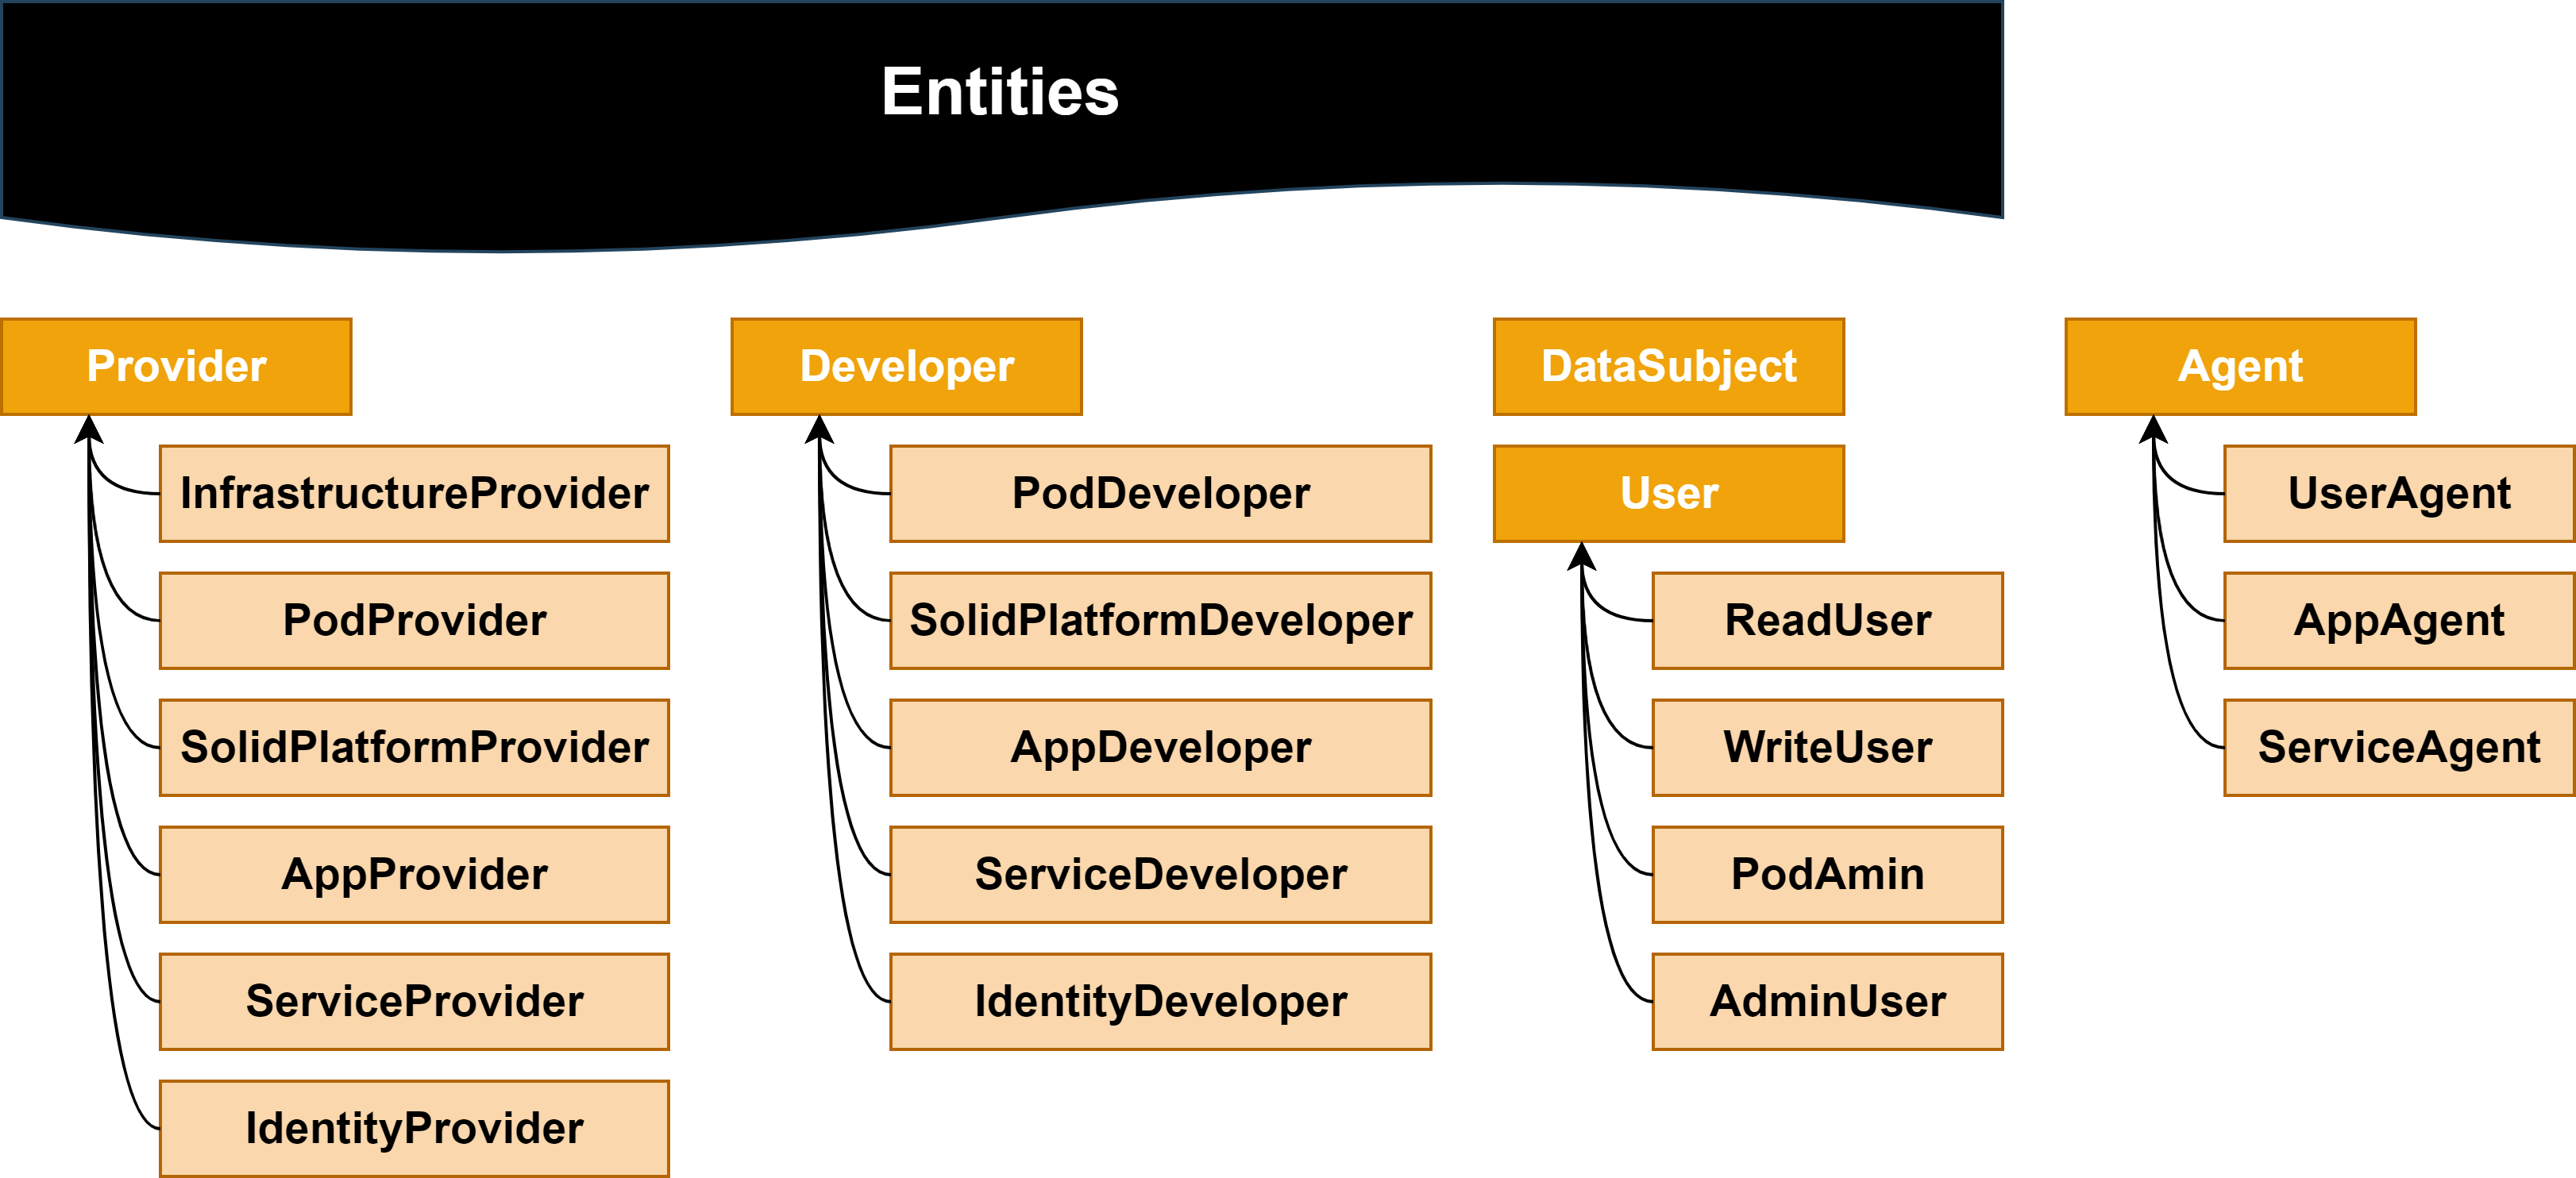
\includegraphics[width=\linewidth]{figures/chapter-4/entities.png}
    \caption{Entities and agents specified in PLASMA.}
    \label{fig:plasma_entities}
\end{figure}

\paragraph{Policies and notices}
In PLASMA, a policy is a document that specifies user, application, and service requirements for data handling practices that apply to data stored or shared through Solid Pods.
Thus, this definition is not limited to access to data stored on a Pod, it also relates to used or transferred data, i.e., to avoid cases such as data collected for purpose X being used for purpose Y.
Such a definition aids with the alignment with legal requirements, e.g., it requires that all purposes must be stated at the time of data collection and that requesters need new consent from the data subject if the purpose for access changes.
PLASMA provides definitions for user policies, in particular for user offers, requirements and preferences, aligned with the \texttt{odrl:Offer}, \texttt{oac:Requirement} and \texttt{oac:Preference} concepts described in Section~\ref{sec:oac}.
Regarding data requests, i.e., conditions for apps and services to have access to or use Pod data, PLASMA envisions their integration into the ecosystem by declaring them in a manifest such as the one being conceived in the W3C Web Application Manifest specification -- an application manifest is a \textit{``JSON document that contains startup parameters and application defaults for when a web application is launched''} \citep{manifest_2023}.
However, the current specification is not enough to achieve legal compliance as it does not include information on entities developing the app, their identity and contact details or their privacy policies.
Thus, PLASMA includes app manifest and service manifest concepts.
In addition to user policies and data requests, PLASMA also provides different types of data agreements, a concept that is completely missing from the Solid specifications as they only provide concepts to refer to apps and users' access authorisations.
As such, an agreement can either be based on the user's consent, or governed by a contract between the user and the entity having responsibility for the app, service or Pod.

Additionally, current Solid specifications also lack the definition of notices.
Notices are documents that provide context information about entities, operations, or data involved in specific processes, e.g., notices may specify the providers, developers, and/or data handling practices of applications and services. 
In this regard, PLASMA provides terms for declaring \textit{ex-ante} and \textit{ex-post} notices, as well as privacy notices for Pods, users, applications and services.

Figure~\ref{fig:plasma_policies} illustrates the policies and notices concepts specified in PLASMA.

\begin{figure}[htb]
    \centering
    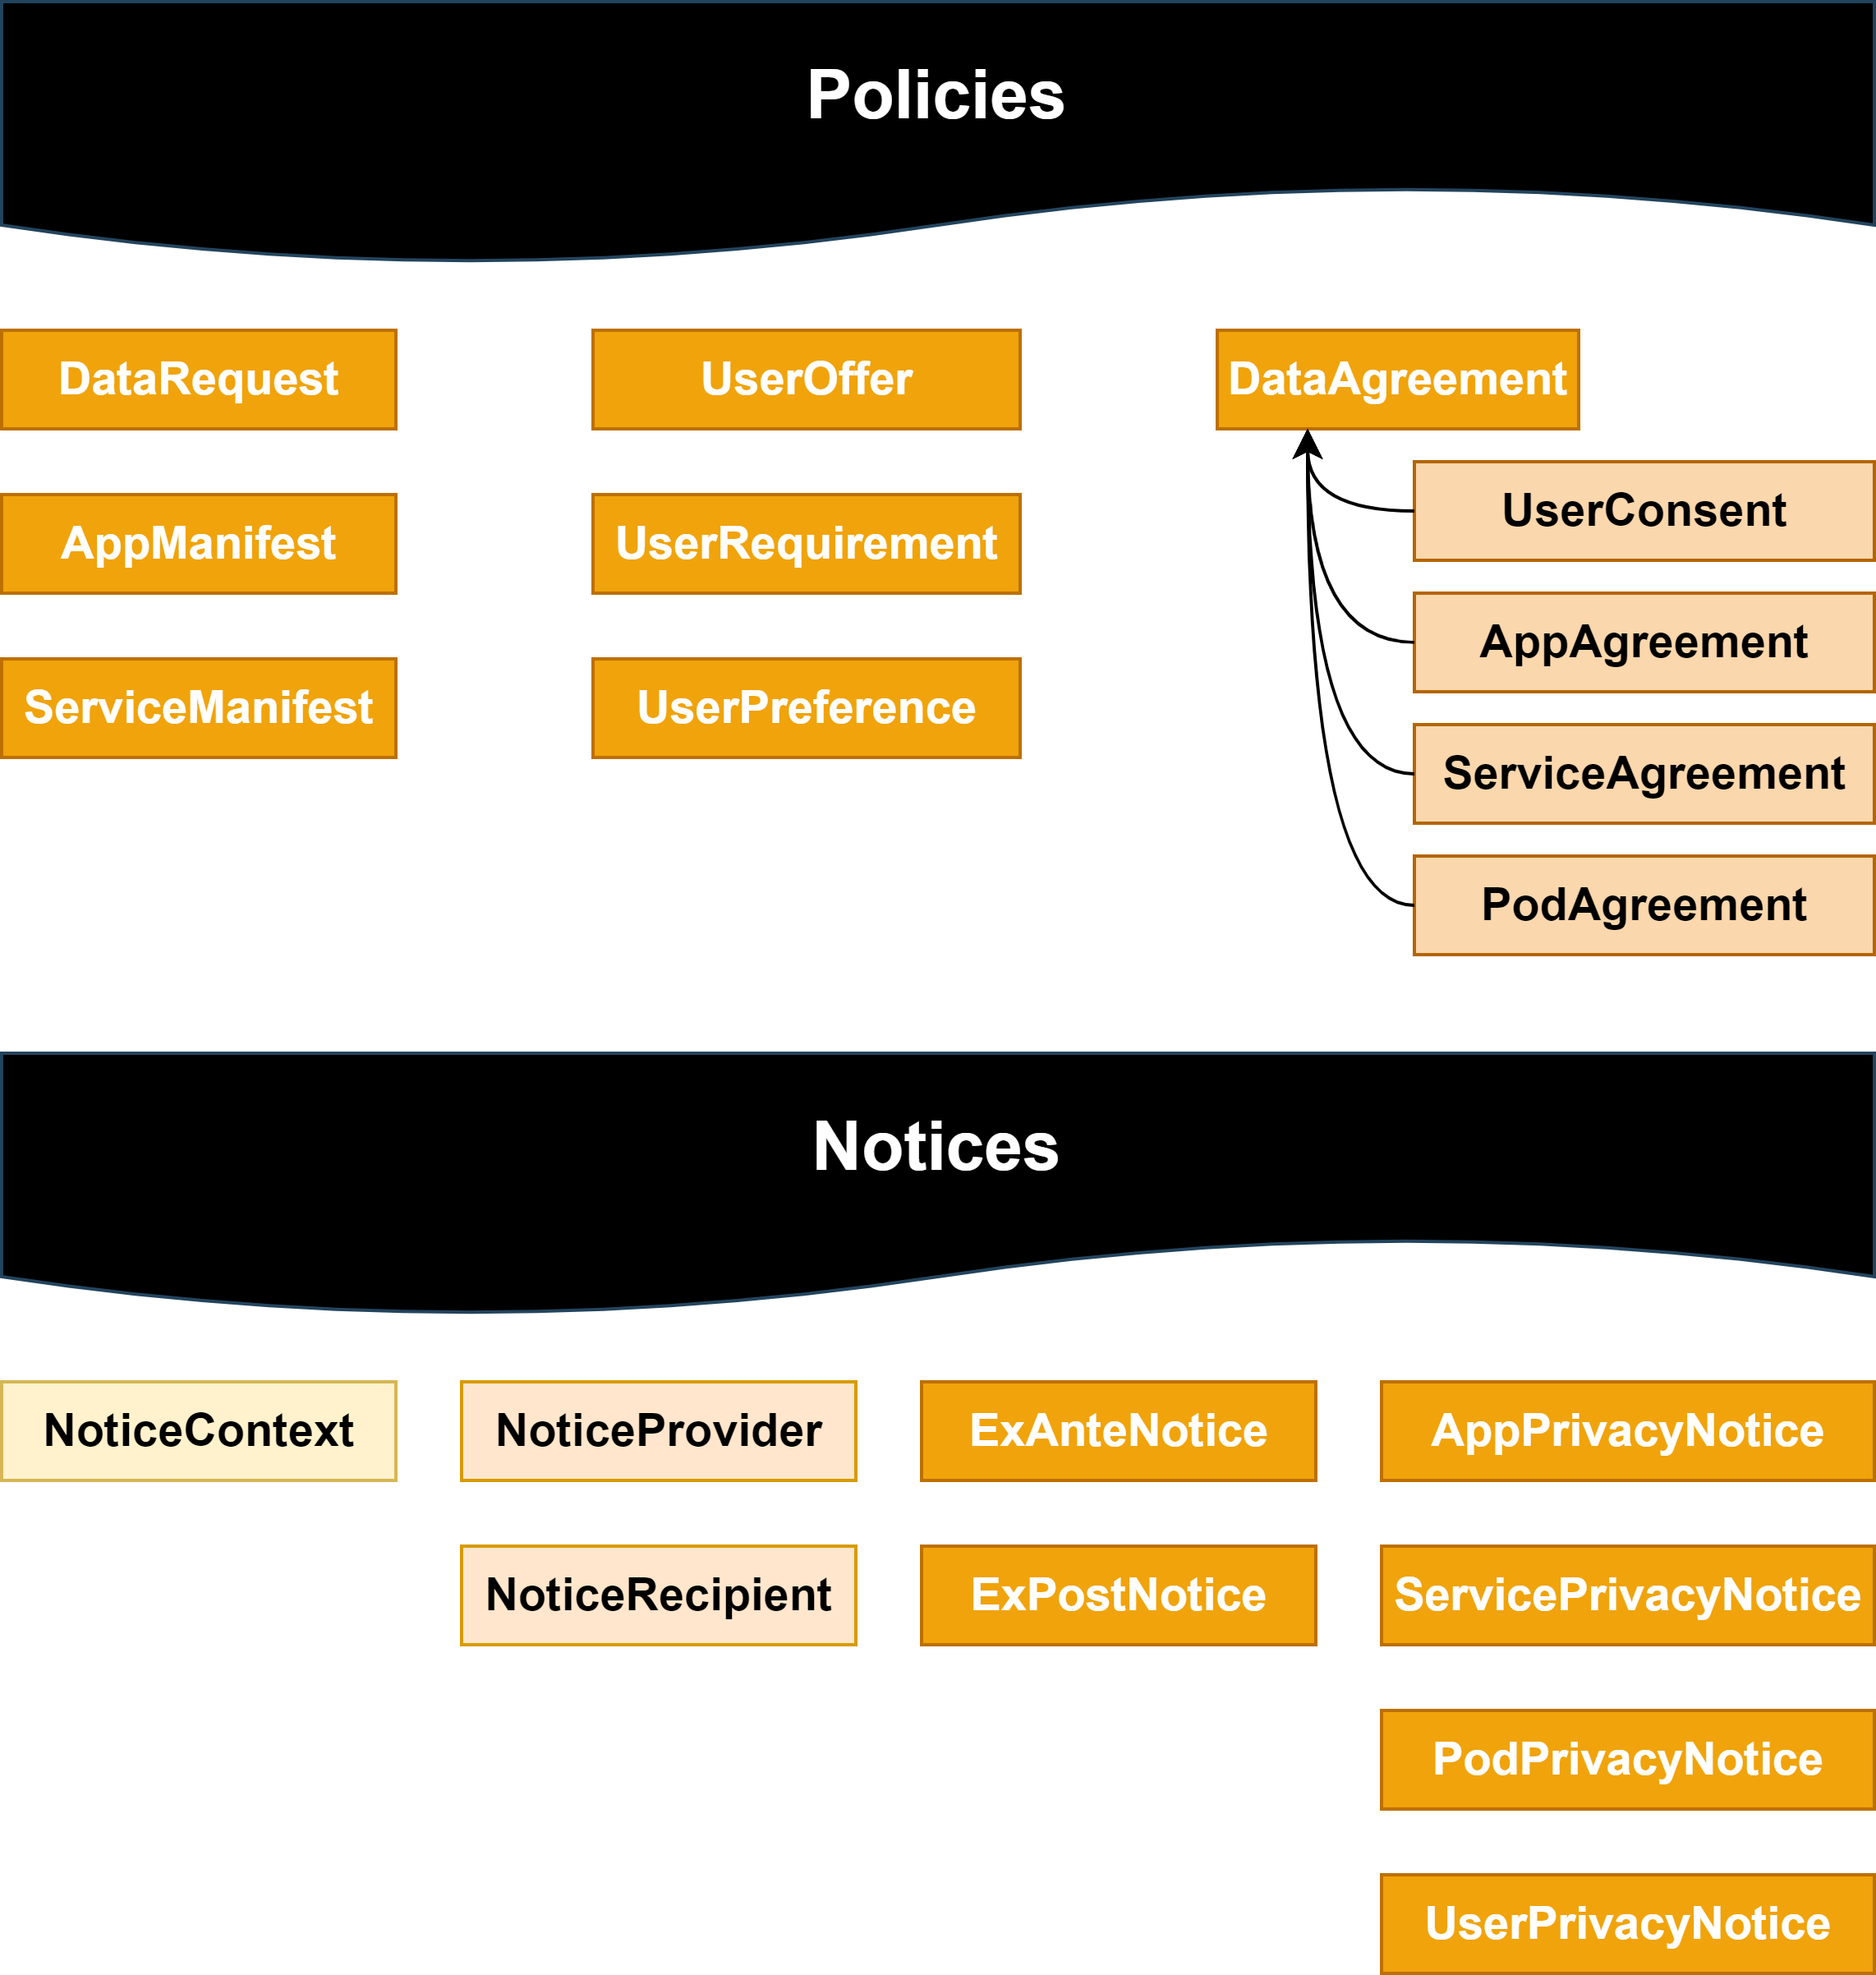
\includegraphics[width=0.8\linewidth]{figures/chapter-4/policies_notices.png}
    \caption{Policy types and notices specified in PLASMA.}
    \label{fig:plasma_policies}
\end{figure}

\paragraph{Services}
PLASMA differentiates between an app and a service -- services convey functionalities that do not need to be packaged as an app.
Moreover, an app requires human intervention to perform some action on data for a specific purpose, while a service may not require human intervention to use or interact with data within a Pod.
Since services are a new concept being introduced by PLASMA in the Solid ecosystem, a taxonomy of twelveu Solid-related services, which can be further expanded, is supplied and illustrated in Figure~\ref{fig:plasma_services}.

\begin{figure}[htb]
    \centering
    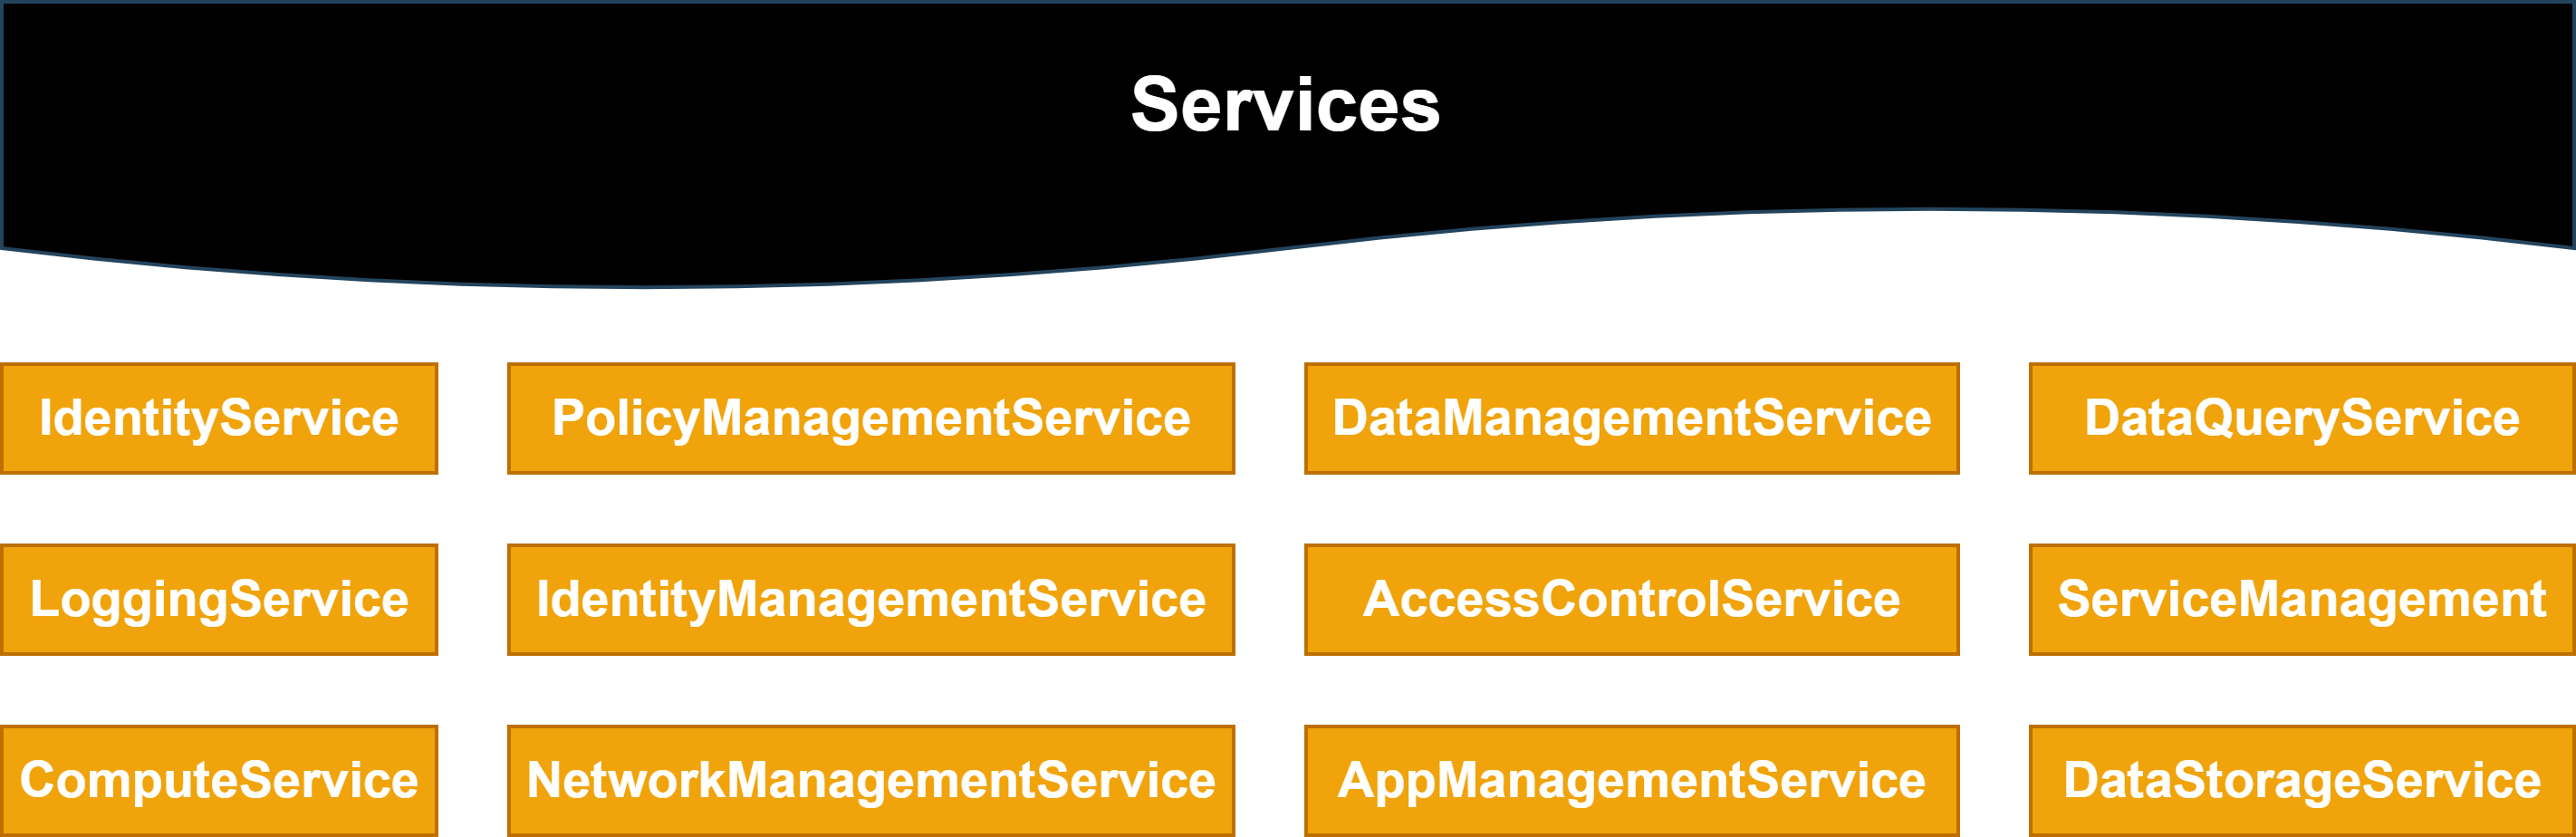
\includegraphics[width=\linewidth]{figures/chapter-4/services.png}
    \caption{Services specified in PLASMA.}
    \label{fig:plasma_services}
\end{figure}

\paragraph{Pod-related data}
To fulfil Solid's vision of providing individuals with a decentralised data storage service for their data and the choice of which applications or services to use for a specific task, metadata regarding Pod management, entities, apps, services, logs and registries should be provided.
Additionally, supervisory authorities can use such logging and provenance metadata, from the Pods of users, for auditing activities, e.g., an EU data protection authority can use these records to investigate a personal data breach.
To this end, PLASMA includes a collection of Solid-related log terms to record provenance information related to processes such as adding or updating resources in a Pod, i.e., a \texttt{DataLog}, registering a policy negotiation procedure reliant on user consent, i.e., a \texttt{PolicyLog}, or recording a successful user login operation, i.e., a \texttt{IdentityLog}.
Furthermore, the maintenance of registries as indexed records for providing collective and convenient access to data within a Pod is of the utmost importance for users, apps and services to have knowledge of the availability of data categories, supported schemas for data, apps, services, relevant policies and users that have/had access to data stored within a Pod.

Figure~\ref{fig:plasma_data} illustrates the Pod-related data concepts defined in PLASMA, including logs and registries.

\begin{figure}[htbp]
    \centering
    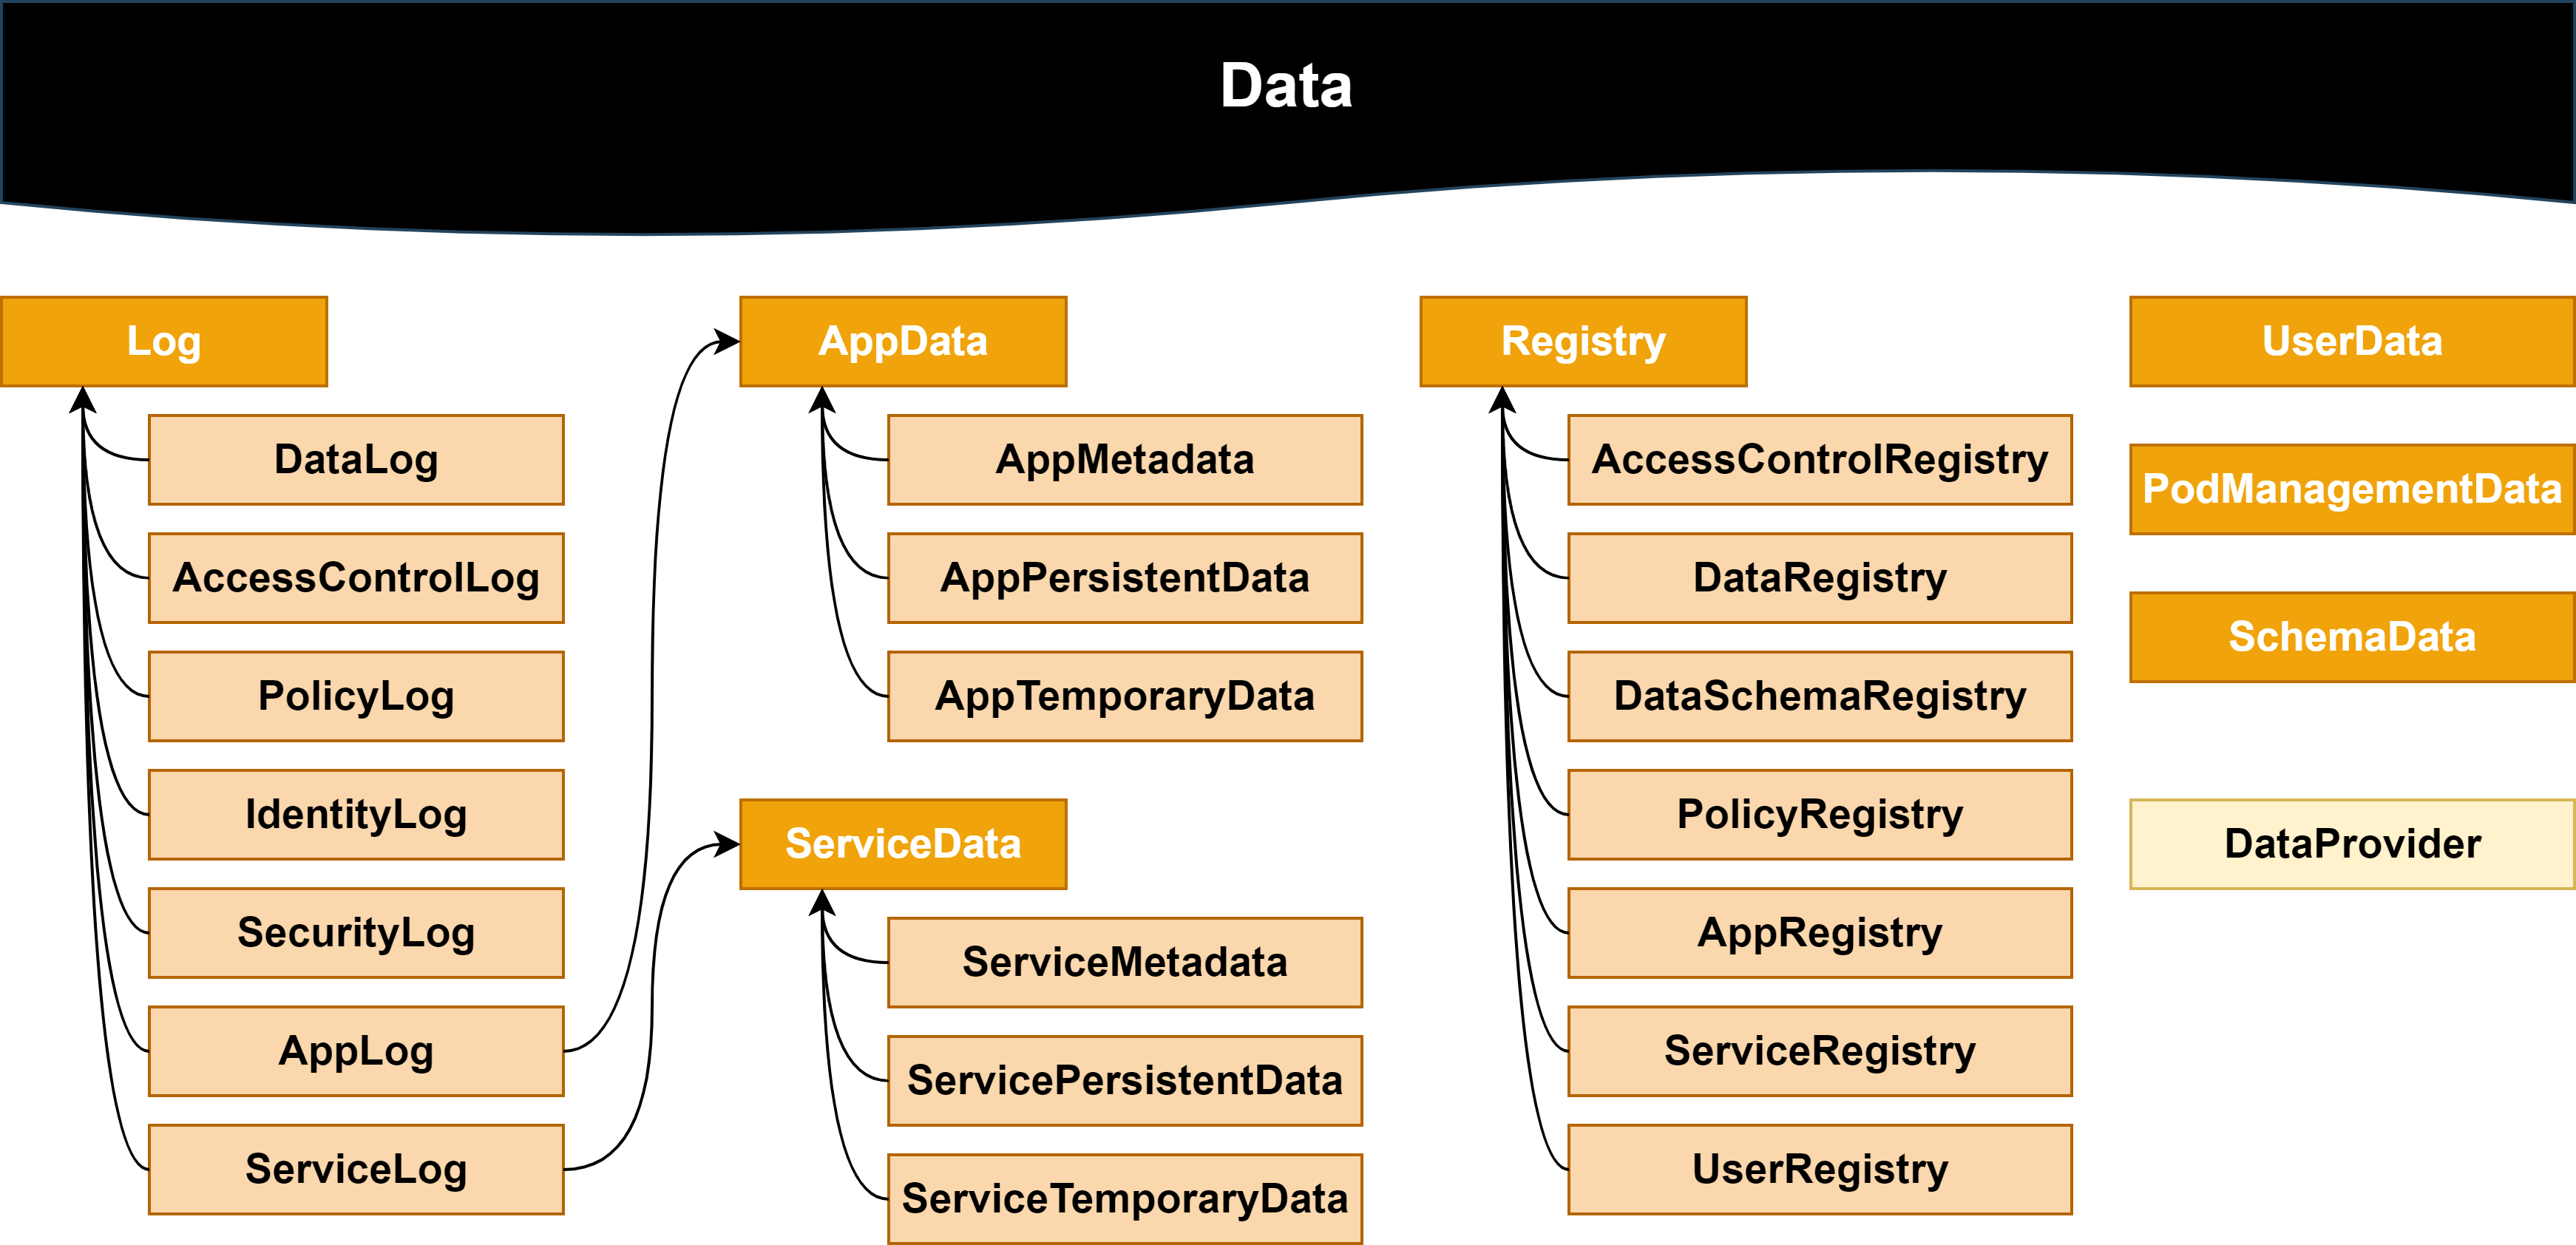
\includegraphics[width=\linewidth]{figures/chapter-4/data.png}
    \caption{Data concepts, including logs and registries, specified in PLASMA.}
    \label{fig:plasma_data}
\end{figure}

\subsection{Conformance with PLASMA}
\label{sec:plasma_conformance}

In this Section, the conditions for Pods, apps, services, users and agents to be conformant with PLASMA are described, including information regarding what is mandatory (indicated below by the use of the word \textit{`must'}) or optional (indicated below by the use of the word \textit{`may'}) to be provided, and how conformity should be evaluated and assured by implementers of the PLASMA specification.

The W3C Recommendation on Data on the Web Best Practices, which is aimed at the \textit{``publication and usage of data on the Web designed to help support a self-sustaining ecosystem''} \citep{loscio_data_2017}, was followed for the publication of metadata related to provenance, licensing and versioning of data.
The vocabulary specifications for particular tasks, recommended by this best practices document, are mentioned in the following paragraphs.

\paragraph{Pod conformance}
For a Pod to be conformant with the PLASMA specification, the following conditions should be satisfied:

\begin{itemize}
    \item A Pod \textit{must} provide or declare \texttt{PodManagementData} which includes metadata about the Pod and of its providers and/or developers, as well as the specific \texttt{SolidPlatform} and \texttt{SolidSpecification} implemented in the Pod and any \texttt{PodAgreement} in place. Listing~\ref{list:plasma_PodManagementData} provides an example of the declaration of such metadata.
    \item A Pod \textit{must} implement or provide equivalent functionality to support the different registries and logs specified in PLASMA. Listing~\ref{list:plasma_dataschemaregistry} provides an example of a data schema registry that records data schemas, formats or shapes recognised or supported by Pods, apps or services, as indicated by the \texttt{plasma:supportedBy} property.
    \item A Pod \textit{may} have multiple users with varying degrees of control. A record of the different users and their level of access \textit{must} be kept in the \texttt{UserRegistry}.
    \item A Pod \textit{may} have discovery methods for users to make their data publicly available.
\end{itemize}

In addition to the ODRL and DCMI Metadata Terms vocabularies, the DPV's \texttt{hasName}, \texttt{hasContact} and \texttt{hasAddress} properties should be used to identify and provide contact details of the Pod, Solid platform and infrastructure providers and developers. \textit{Schema.org} and the Provenance, Authoring and Versioning (PAV) vocabularies, along with the previously mentioned DCMI, are used to describe the authors, sources, version and code repository URIs of the platform and specification installed within the Pod. \textit{Schema.org} provides an upper vocabulary of terms to describe \textit{``entities, relationships between entities and actions''} related to structured data on the Web \citep{guha_schemaorg_2015} and PAV is a \textit{``lightweight ontology for tracking Provenance, Authoring and Versioning''} that \textit{``specializes the W3C provenance ontology PROV-O in order to describe authorship, curation and digital creation of online resources''} \citep{ciccarese_pav_2013}.

\begin{listing}[htp]
\caption{Metadata of Beatriz's Pod.}
\label{list:plasma_PodManagementData}
\begin{minted}{turtle}
<https://solidweb.me/besteves4/PodMetadata> a plasma:PodManagementData ;
    dcterms:description "Metadata of Beatriz's Pod" ;
    odrl:hasPolicy <https://solidweb.me/besteves4/agreements/Pod> ;
    plasma:hasProvider <https://solidweb.me/besteves4/entities/PodProvider> ;
    plasma:hasProvider <https://solidweb.me/besteves4/entities/PlatformProvider> ;
    plasma:hasProvider <https://solidweb.me/besteves4/entities/InfrastructureProvider> ;
    plasma:implementedSolidPlatform <https://solidweb.me/besteves4/Platform> ;
    plasma:implementedSolidSpecification <https://solidweb.me/besteves4/SolidSpec> .

<https://solidweb.me/besteves4/agreements/Pod> a plasma:PodAgreement .

<https://solidweb.me/besteves4/entities/PodProvider> a plasma:PodProvider ;
    dpv:hasName "Entity A" ; dpv:hasContact "mailto:entity_a@mail.com" ;
    dpv:hasAddress "Address of Entity A" .

<https://solidweb.me/besteves4/entities/PlatformProvider> a plasma:SolidPlatformProvider .

<https://solidweb.me/besteves4/entities/InfrastructureProvider> a plasma:InfrastructureProvider .

<https://solidweb.me/besteves4/Platform> a plasma:SolidPlatform ;
    plasma:hasProvider <https://solidweb.me/besteves4/entities/PlatformProvider> ;
    dcterms:source <https://communitysolidserver.github.io> ;
    dpv:hasPolicy <https://www.serverproject.de/files/solidweb_me_terms.txt> ;
    schema:codeRepository <https://github.com/CommunitySolidServer/CommunitySolidServer> ;
    pav:version "6.1.0" ;
    dcterms:license <https://dalicc.net/licenselibrary/MIT> .

<https://solidweb.me/besteves4/SolidSpec> a plasma:SolidSpecification ;
    dcterms:conformsTo <https://solidproject.org/TR/2022/protocol-20221231> ;
    dcterms:creator "Sarven Capadisli", "Tim Berners-Lee", "Ruben Verborgh", "Kjetil Kjernsmo" ;
    dcterms:license <https://dalicc.net/licenselibrary/MIT> ;
    pav:version "0.10.0" ; dcterms:created "2022-12-31"^^xsd:date ;
    schema:codeRepository <https://github.com/solid/specification> .
\end{minted}
\end{listing}

\begin{listing}[htp]
\caption{Data schema registry of Beatriz's Pod.}
\label{list:plasma_dataschemaregistry}
\begin{minted}{turtle}
<https://solidweb.me/besteves4/SchemaRegistry> a plasma:DataSchemaRegistry ;
    dcterms:description "Registry listing recognised or supported schemas" ;
    dcterms:created "2023-09-10T11:51:17"^^xsd:dateTime ;
    dcterms:modified "2023-10-07T12:39:50"^^xsd:dateTime ;
    dcterms:publisher <https://solidweb.me/besteves4/entities/DataMgtServiceProvider> ;
    plasma:hasSchema <https://solidweb.me/besteves4/schemas/EHR-schema>,
        <https://solidweb.me/besteves4/schemas/img-format>,
        <https://solidweb.me/besteves4/schemas/entity-shape> .

<https://solidweb.me/besteves4/entities/DataMgtServiceProvider> a plasma:ServiceProvider ;
    plasma:serviceType plasma:DataManagementService ;
    dpv:hasName "Entity A" ;
    dpv:hasAddress "Address of Entity A" ;
    dpv:hasContact "mailto:entity_a@mail.com" .

<https://solidweb.me/besteves4/schemas/EHR-schema> a plasma:SchemaData ;
    dcterms:conformsTo <http://www.w3.org/TR/turtle/> ;
    plasma:supportedBy <https://example.com/health-service> .

<https://example.com/health-service> a plasma:Service .

<https://solidweb.me/besteves4/schemas/img-format> a plasma:SchemaData ;
    dcterms:format <https://www.iana.org/assignments/media-types/image/png>,
        <https://www.iana.org/assignments/media-types/image/svg+xml> ;
    plasma:supportedBy <https://example.com/social-app> .

<https://example.com/social-app> a plasma:App .

<https://solidweb.me/besteves4/schemas/entity-shape> a plasma:SchemaData, sh:NodeShape ;
    plasma:supportedBy <https://solidweb.me/besteves4/> ;
    sh:name "PLASMA entity shape" ;
    sh:description "Minimum data that PLASMA entities should provide to be identified." ;
    sh:targetClass plasma:Entity .
\end{minted}
\end{listing}

% software description: https://w3id.org/okn/o/sd
% paper: Towards Assessing FAIR Research Software Best Practices in an Organization Using RDF-star. Ana Iglesias-Molina and Daniel Garijo

\paragraph{Apps and services conformance}
For an app or service to be conformant with the PLASMA specification, the following conditions should be satisfied:

\begin{itemize}
    \item An app, or service, \textit{must} have an \texttt{AppManifest}, or \texttt{ServiceManifest}, in conformance with the W3C Web Application Manifest \citep{manifest_2023}. A Pod \textit{may} ensure manifest conformance using SHACL shapes. Listing~\ref{list:plasma_appmanifest} provides an example of an app manifest.
    \item An \texttt{AppManifest}, or \texttt{ServiceManifest}, \textit{must} include information regarding the developer and provider of legally relevant entities and their identities.
    \item An \texttt{AppManifest}, or \texttt{ServiceManifest}, \textit{must} state the \texttt{DataRequest} representing the request to use data using the \texttt{odrl:hasPolicy} property. The request \textit{must} provide all information regarding the use of data even if only some of it will be applicable initially or used in the notice.
    \item An \texttt{AppManifest}, or \texttt{ServiceManifest}, \textit{must} link the privacy notice of the app, or service, using the \texttt{dpv:hasNotice} property. The Pod \textit{may} use this information to display or optionally construct its own notice based on the preferences or accessibility requirements of the user.
    \item An \texttt{AppManifest}, or \texttt{ServiceManifest}, \textit{must} be stored in the Pod \texttt{AppRegistry}, or \texttt{ServiceRegistry}. Listing~\ref{list:plasma_appregistry} provides an example of an app registry, where app-related metadata, including the manifest, app providers and developers, temporary or persistent app data, is recorded.
    \item Apps, or services, \textit{may} have multiple \texttt{AppAgents}, or \texttt{ServiceAgents}, which \textit{must} be registered in the \texttt{AppRegistry}, or \texttt{ServiceRegistry}.
\end{itemize}

In addition to the PLASMA terms mentioned in the previous list, the usage of the \texttt{plasma:serviceType} property can be used to connect service providers and developers with a particular type of service, e.g., from PLASMA's service taxonomy, that is provided or developed by said entity.
Moreover, it should be noted that app or service stores, such as those maintained by Apple and Google, can also act as app or service providers and the FOAF \texttt{page} property can be used to actually connect the store provider with the store itself.
The FOAF vocabulary specification \citep{brickley_foaf_2004} provides terms to describe people and related personal information and online accounts.
Regardless, support for other optional properties specified in the W3C Web Application Manifest specification, such as icons, display mode, orientation, and background colour, can also be integrated into the modelled manifests, as well as `common' app store metadata, such as screenshots, user rating or app type, e.g., health, game or news app \citep{gustafson_web_2023}.

\begin{listing}[htp]
\caption{App manifest of Contacts app.}
\label{list:plasma_appmanifest}
\begin{minted}{turtle}
<https://example.com/Contacts> a plasma:App ;
    plasma:hasAppManifest <https://example.com/Contacts/Manifest> .

<https://example.com/Contacts/Manifest> a plasma:AppManifest ;
    dcterms:conformsTo <https://www.w3.org/TR/appmanifest/> ;
    dcterms:issued "2023-10-23T22:43:58"^^xsd:dateTime ;
    dcterms:title "Contacts" ;
    dcterms:description "App to manage contacts" ;
    dcterms:language <http://id.loc.gov/vocabulary/iso639-1/en> ;
    plasma:hasProvider <https://solidweb.me/besteves4/entities/AppStore> ;
    plasma:hasDeveloper <https://solidweb.me/besteves4/entities/ContactsDeveloper> ;
    odrl:hasPolicy <https://example.com/Contacts/Request> ;
    dpv:hasNotice <https://example.com/Contacts/Notice> .

<https://solidweb.me/besteves4/entities/AppStore> a plasma:AppProvider ;
    dpv:hasName "App Store provider" ;
    dpv:hasAddress "Address of App Store provider" ;
    dpv:hasContact "mailto:app_store@mail.com" ;
    foaf:page <https://example.com/AppStore> ;
    dpv:hasNotice <https://example.com/AppStore/PrivacyPolicy> .

<https://solidweb.me/besteves4/entities/ContactsDeveloper> a plasma:AppDeveloper .

<https://example.com/Contacts/request> a plasma:DataRequest, odrl:Request .
\end{minted}
\end{listing}

\begin{listing}[htp]
\caption{App registry of Beatriz's Pod.}
\label{list:plasma_appregistry}
\begin{minted}{turtle}
<https://solidweb.me/besteves4/AppRegistry> a plasma:AppRegistry ;
    dcterms:description "Registry listing apps" ;
    dcterms:created "2023-09-30T11:33:35"^^xsd:dateTime ;
    dcterms:modified "2023-10-07T11:31:40"^^xsd:dateTime ;
    dcterms:publisher <https://solidweb.me/besteves4/entities/AppMgProvider> ;
    plasma:hasApp <https://solidweb.me/besteves4/apps/Contacts/> .

<https://solidweb.me/besteves4/entities/AppMgProvider> a plasma:ServiceProvider ;
    plasma:serviceType plasma:AppManagementService .

<https://solidweb.me/besteves4/apps/Contacts/> a plasma:App ;
    plasma:hasAppManifest <https://solidweb.me/besteves4/apps/Contacts/Manifest> ;
    odrl:hasPolicy <https://solidweb.me/besteves4/apps/Contacts/Agreement> ;
    plasma:hasAppMetadata <https://solidweb.me/besteves4/apps/Contacts/Metadata> ;
    plasma:hasAppPersistentData <https://solidweb.me/besteves4/apps/Contacts/PersistentData> ;
    plasma:hasAppTemporaryData <https://solidweb.me/besteves4/apps/Contacts/TemporaryData> ;
    plasma:hasAgent <https://solidweb.me/besteves4/apps/Contacts/Agent> .

<https://solidweb.me/besteves4/apps/Contacts/Metadata> a plasma:AppMetadata ;
    dcterms:description "Contacts metadata" ;
    plasma:hasProvider <https://solidweb.me/besteves4/entities/AppStore> ;
    plasma:hasDeveloper <https://solidweb.me/besteves4/entities/ContactsDeveloper> .

<https://solidweb.me/besteves4/apps/Contacts/PersistentData> a plasma:AppPersistentData ;
    dcterms:type dpv-pd:TelephoneNumber ; rdf:value "(+34)691485135" .

<https://solidweb.me/besteves4/apps/Contacts/TemporaryData> a plasma:AppTemporaryData ;
    dcterms:type dpv-pd:TelephoneNumber ; rdf:value "(+34)691998745" ;
    dcterms:valid "2023-10-01T14:50:21"^^xsd:dateTime .

<https://solidweb.me/besteves4/apps/Contacts/Agent> a plasma:AppAgent .
\end{minted}
\end{listing}

\paragraph{User conformance}
For a user to be conformant with the PLASMA specification, the following conditions should be satisfied:

\begin{itemize}
    \item Impactful interactions of a user, e.g., changing identity providers, \textit{must} be recorded using a well-defined shape. Listing~\ref{list:plasma_accesscontrollog} provides an example of access control logs modelled with PLASMA and using W3C's Activity Streams activity types \citep{snell_activity_2017}.
    \item A \texttt{UserRegistry} \textit{must} contain information regarding the \texttt{DataSubjects} storing data within a Pod, the \texttt{PodAdmin} and other users accessing Data. Listing~\ref{list:plasma_userregistry} provides an example of said registry.
    \item Users \textit{may} be directly associated with a \texttt{DataRequest} so that they can make requests for data without using an application or service.
    \item Users \textit{may} have multiple \texttt{UserAgents}, which should be registered in the \texttt{UserRegistry}.
\end{itemize}

PLASMA recommends the usage of the W3C's Activity Streams vocabulary \citep{snell_activity_2017} to model the distinct logs that should be stored in Solid Pods for transparency and accountability, e.g., data, identity or policy logs.
This recommendation provides an extensive list of activity, actor and object types that provides ``a baseline extensible syntax for the expression of completed activities''.
Such syntax allows the identification of the resource being logged, using the \texttt{as:object} property, the entity responsible for the activity being logged, using the \texttt{as:actor} property, or the app or service used to generate the log, employing the \texttt{as:generator} property.
The \texttt{as:Accept} and \texttt{as:Reject} activity types can be reused to express when access to data or policies are accepted or rejected, and the \texttt{as:Create}, \texttt{as:Update}, \texttt{as:Delete} and \texttt{as:Move} activities can be reused to log the creation, modification, deletion or movement of data or policies.
New activity types, e.g., to request data, change identity providers or verify the identity of apps, which are not modelled by the Activity Streams vocabulary, are modelled in PLASMA, e.g., as \texttt{plasma:Request}, \texttt{plasma:ChangeIdP} or \texttt{plasma:Verify}.

It should also be stated that Inrupt's Enterprise Solid Server has started to provide an auditing service\footnote{\url{https://docs.inrupt.com/ess/latest/services/service-auditing/} (accessed on 21 December 2023)} which also relies on the W3C Activity Streams 2.0 Recommendation \citep{snell_activity_2017} to document audit events related with the identity of user and applications.

\begin{listing}[htp]
\caption{Access control logs recorded in Beatriz's Pod.}
\label{list:plasma_accesscontrollog}
\begin{minted}{turtle}
<https://solidweb.me/besteves4/logs/AccessControl_Reject> a plasma:AccessControlLog ;
	dcterms:type as:Reject ;
	dcterms:issued "2023-11-12T15:34:04"^^xsd:dateTime ;
	as:summary "Access to data rejected" ;
	as:object <https://solidweb.me/besteves4/health/ehr> ;
	as:actor <https://solidweb.me/arya/profile/card#me> ;
	as:generator <https://example.com/App> ;
	dcterms:publisher <https://solidweb.me/besteves4/entities/LoggingProvider> .

<https://solidweb.me/besteves4/logs/AccessControl_Accept> a plasma:AccessControlLog ;
	dcterms:type as:Accept ;
	dcterms:issued "2023-11-12T15:43:09"^^xsd:dateTime ;
	as:summary "Access to data accepted" ;
	as:object <https://solidweb.me/besteves4/contacts/> ;
	as:actor <https://solidweb.me/arya/profile/card#me> ;
	as:generator <https://example.com/App> ;
	dcterms:publisher <https://solidweb.me/besteves4/entities/LoggingProvider> .

<https://example.com/App> a plasma:App .

<https://solidweb.me/besteves4/entities/LoggingProvider> a plasma:ServiceProvider ;
	plasma:serviceType plasma:LoggingService ;
	dpv:hasName "Entity G" ;
	dpv:hasAddress "Address of Entity G" ;
	dpv:hasContact "mailto:entity_g@mail.com" .
\end{minted}
\end{listing}

\begin{listing}[htp]
\caption{User registry of Beatriz's Pod.}
\label{list:plasma_userregistry}
\begin{minted}{turtle}
<https://solidweb.me/besteves4/UserRegistry> a plasma:UserRegistry ;
    dcterms:description "Registry listing users" ;
    dcterms:created "2023-09-30T11:33:35"^^xsd:dateTime ;
    dcterms:modified "2023-10-07T12:39:50"^^xsd:dateTime ;
    dcterms:publisher <https://solidweb.me/besteves4/entities/UserMProvider> ;
    dpv:hasDataSubject <https://solidweb.me/besteves4/entities/DataSubject> ;
    plasma:hasUser <https://solidweb.me/besteves4/entities/DataSubject>,
        <https://solidweb.me/besteves4/entities/ReadUserA>,
        <https://solidweb.me/besteves4/entities/ReadUserB>,
        <https://solidweb.me/besteves4/entities/Admin> .

<https://solidweb.me/besteves4/entities/UserMProvider> a plasma:ServiceProvider ;
    dpv:hasName "Entity A" ;
    dpv:hasAddress "Address of Entity A" ;
    dpv:hasContact "mailto:entity_a@mail.com" .

<https://solidweb.me/besteves4/entities/DataSubject> a plasma:DataSubject, plasma:PodAdmin ;
    dpv:hasName "Data Subject" ;
    dpv:hasAddress "Address of Data Subject" ;
    dpv:hasContact "mailto:data_subject@mail.com" ;
    plasma:hasAgent <https://solidweb.me/besteves4/agents/AgentA> .

<https://solidweb.me/besteves4/agents/AgentA> a plasma:UserAgent .

<https://solidweb.me/besteves4/entities/ReadUserA> a plasma:ReadUser ;
    plasma:hasPolicy <https://solidweb.me/besteves4/requests/UserA> .

<https://solidweb.me/besteves4/entities/UserA> a plasma:DataRequest .

<https://solidweb.me/besteves4/entities/ReadUserB> a plasma:ReadUser ;
    plasma:hasPolicy <https://solidweb.me/besteves4/requests/UserB> ;
    plasma:hasPolicy <https://solidweb.me/besteves4/agreements/UserB> .

<https://solidweb.me/besteves4/agreements/UserB> a odrl:Agreement, plasma:UserConsent .

<https://solidweb.me/besteves4/entities/Admin> a plasma:AdminUser .
\end{minted}
\end{listing}

\paragraph{Agent conformance}
For an agent to be conformant with the PLASMA specification, the following conditions should be satisfied:

\begin{itemize}
    \item Agents activity \textit{must} be in accordance with the manifest of the entity for which they are acting on behalf of.
    \item A record of the usage of an \texttt{AppAgent}, \texttt{ServiceAgent} or \texttt{UserAgent} \textit{must} be kept in the \texttt{AppRegistry}, \texttt{ServiceRegistry} or \texttt{UserRegistry}, respectively, including information regarding its providers/developers for accountability. User \url{https://solidweb.me/besteves4/entities/DataSubject} in Listing~\ref{list:plasma_userregistry} has a user agent identified with the PLASMA property \texttt{hasAgent}.
\end{itemize}

Finally, each of the requirements established in the previous paragraphs for the conformance of Pods, apps, services, users and agents with PLASMA should be verified using a language for describing and validating RDF graphs.
As such, SHACL can, not only, be used for the definition of data shapes recognised or supported by apps, services or Pods, but also can act as a general tool to verify conformance with the conditions specified in this Section.
SHACL was chosen for this conformance checking since it is a widely used and supported W3C Recommendation for \textit{``validating RDF graphs against a set of conditions''} \citep{knublauch_shapes_2017}.
SHACL shapes for all the previously mentioned conformance conditions were generated in this Thesis and are provided in the Appendix.

% SHACL shapes generator: https://github.com/AKSW/shaclgen

% PLASMA is available at \url{https://w3id.org/plasma}, under the CC-By-4.0 license, and reuses the available terms in the Solid vocabularies, when appropriate, in line with FAIR (Findable, Accessible, Interoperable, Reusable) principles. Each taxonomy is discussed below.

% Externally, `app stores' such as those maintained by Apple and Google and `package repositories' such as those maintained by Linux distributions also feature the use of metadata that developers must provide in order for their apps to be enlisted in their stores. These platforms also use this metadata for governing apps, identifying compatibility, and enforcing guidelines.

\subsection{Vocabulary publication and maintenance}
\label{sec:plasma_publication}

The vocabulary human-readable documentation and machine-readable file are available at \url{https://w3id.org/plasma} using content negotiation.
The HTML documentation includes a description of the terms defined in PLASMA, which was conducted and validated with domain experts, diagrams with graphical representations of the several taxonomies included in the vocabulary, a detailed explanation of the conformance conditions that need to be adopted by Pods, apps, services, agents and users for them to be PLASMA-compliant, RDF examples of workflows that use PLASMA terms for specific scenarios, e.g., creating user policies or auditing Pods, and information related to legal compliance.
The vocabulary documentation also includes metadata, such as the identity of the creators and publishers of the ontology, the dates of creation and last modification or the version number.

The source code is hosted at \url{https://w3id.org/plasma/repo}, under the CC-BY-4.0 license.
The repository can also be used by PLASMA implementers to suggest new inclusions to the vocabulary and to report bugs through GitHub Issues.
\section{Exercising data subject rights with DPV}
\label{sec:rights_exercising}

This Section describes the usage of vocabulary-based patterns to describe rights exercising metadata.
Such patterns can be used by entities dealing with the handling of personal data to maintain consistent records of data subject rights exercising activities, aligned with GDPR requirements.
In a decentralised data system environment, these rights must also be fulfilled by data controllers, while notices and records of rights exercising activities can be kept by data subjects in their personal datastores for transparency and accountability.

\subsection{Requirements to express rights-related activities}
\label{sec:rights_concepts}

This Section outlines the motivation and identified requirements for the expression of information related to the exercising of data subject rights.
This work was developed (and is already integrated) within the context of the DPVCG and was started with the main objectives of indicating (i) what rights exist (in particular within the framework of the GDPR), (ii) where such rights can be exercised, and (iii) what information needs to be recorded and maintained when a concrete instance of a right is being/was exercised.

As previously mentioned in Section~\ref{sec:def_gdpr} and represented in Figure~\ref{fig:gdpr_information_flows}, the focus of this Thesis is on the representation of information related to legislation on data protection in the European Union, in particular regarding the GDPR and related data subject rights, listed on Chapter III.
Moreover, in Section~\ref{sec:sota_vocabularies_criteria}, and in particular in Table~\ref{tab:GDPR_privacy_terms}, the privacy terms that need to be represented for such rights to be exercised by data subjects and fulfilled by data controllers.

Figure~\ref{fig:gdpr-rights} illustrates the flows of information between a data subject and a data controller for the exercising of a right request, according to the GDPR.
After sending a notice to the data subject confirming that the request was received, the controller must be able to identify the data subject in order to proceed with the request~(Article 12.2, second sentence~\citeyearpar{noauthor_regulation_2016}).
If the controller cannot identify the data subject, then the data subject must provide additional information to enable the controller to identify them~(Article 11.2~\citeyearpar{noauthor_regulation_2016}).
If the controller disregards the request or has a justification for not fulfilling the right, then the data subject does not receive any information related to the right request~(Article 12.2, second sentence~\citeyearpar{noauthor_regulation_2016}).
In case the controller has a justification to delay the request due to its complexity or a high number of requests, then the controller has a 2-month extension to fulfil its duty~(Article 12.3,
second sentence~\citeyearpar{noauthor_regulation_2016}).
Moreover, in case the request is unfounded or excessive, the controller can charge a fee and the data subject will get the information once this fee is paid~(Article 12.5, first sentence~\citeyearpar{noauthor_regulation_2016}).
As it is visible by the diagram, at any point if the data controller does not fulfil its duty then a GDPR breach occurs and the data subject does not receive their requested information.

% this could be clearer as a uml process diagram with separate swim lanes for subject and controller to clarify which does which activities and decision and also to clarify the start and end states of the flow.
\begin{figure}[htp]
    \centering
    \includegraphics[width=0.78\linewidth]{figures/chapter-4/GDPR-DSR.png}
    \caption[Flow diagram of GDPR data subject rights exercising.]{Flow diagram of GDPR data subject rights exercising, according to Article 12.}
    \label{fig:gdpr-rights}
\end{figure}

From the analysis of these flows of information, a set of high-level concepts was proposed and adopted by the DPVCG (general concepts on Rights are modelled in the main DPV specification at \url{https://w3id.org/dpv#vocab-rights} and GDPR-specific ones in the DPV-GDPR extension at \url{https://w3id.org/dpv/legal/eu/gdpr#vocab-rights}\footnote{The concepts that have `Beatriz Esteves' has a contributor are an outcome of this Thesis}).
Figure~\ref{fig:rights_dpv}, adapted from \cite{pandit_primer_2022}, provides an overview of these concepts.

\begin{figure}[ht]
    \centering
    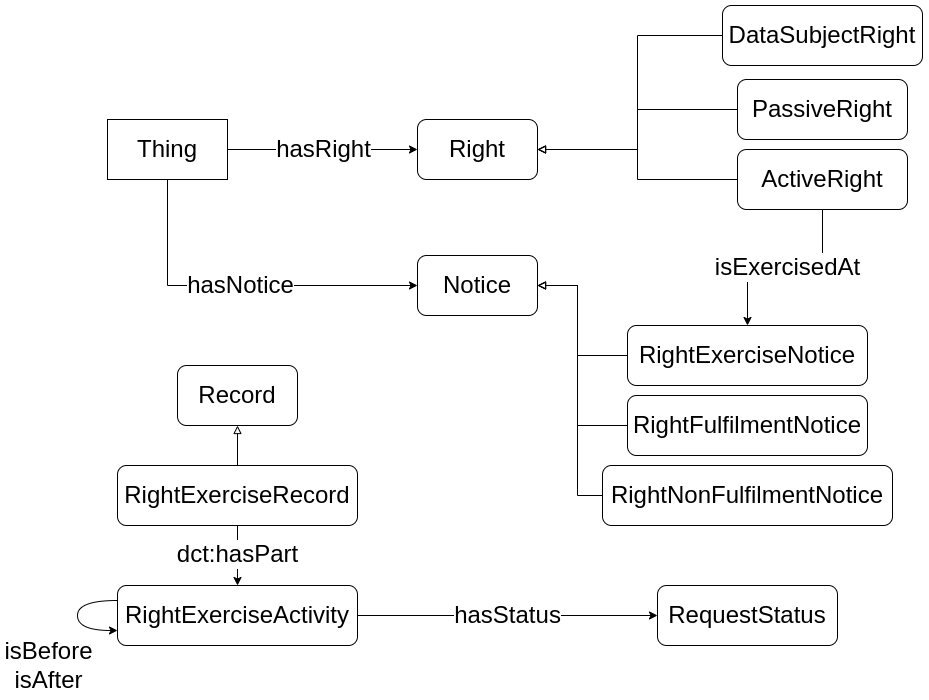
\includegraphics[width=0.8\linewidth]{figures/chapter-4/DPV-rights.png}
    \caption[Core concepts of DPV's rights taxonomy.]{Core concepts of DPV's rights taxonomy, adapted from \cite{pandit_primer_2022}.}
    \label{fig:rights_dpv}
\end{figure}

Thus, beyond modelling concepts for applicable \texttt{Right}s and \texttt{DataSubjectRight}s (applicable only to data subjects), to indicate the association of concepts with a particular right, the \texttt{hasRight} property is also modelled in DPV.
Additionally, to make a distinction between actionable and non-actionable rights, the \texttt{ActiveRight} and \texttt{PassiveRight} concepts were created to distinguish between rights that require an action to be taken for them to be exercised and rights that don't require any action and are always applicable.% add examples of active/passive rights
To fulfil the second objective of establishing where such active rights can be exercised, DPV's \texttt{isExercisedAt} property should be used to connect the right with the \texttt{RightExerciseNotice}.
This notice provides contextual information regarding how to exercise a right.
Specialised notice concepts for rights that can be fulfilled and those that cannot are modelled as \texttt{RightFulfilmentNotice} and \texttt{RightNonFulfilmentNotice}, respectively.

Moreover, to represent concrete records of rights being exercised, the \texttt{RightExerciseRecord} concept, specified as a subclass of DPV's \texttt{Record}, can be used to associate a particular request, or even distinct requests from the same data subject, with corresponding rights exercising activities, modelled as \texttt{RightExerciseActivity}, using the DCMI Metadata Terms \texttt{hasPart} property.
Such activity instances should include metadata, e.g., timestamps, duration, or involved entities, to track the provenance of a particular right exercising process, from the request itself to its acknowledgement by the data controller and to the fulfilment or non-fulfilment of the right.

In order to justify a certain right exercise activity, a collection of justifications for the non-fulfilment, i.e., \texttt{RightNonFulfilmentJustification}, delay of fulfilment, i.e.,\linebreak \texttt{RightFulfilmentDelayJustification}, and exercise of rights, i.e.,\linebreak \texttt{RightExerciseJustification}, were modelled as subclasses of the\linebreak \texttt{NonPerformanceJustification}, \texttt{DelayJustification}, and\linebreak \texttt{ExerciseJustification} concepts, which were modelled to have generic justification concepts that can be used beyond the rights domain.
\texttt{NotRequiredJustification}s are also modelled for when a certain request is not required as it does not apply. 
Figure~\ref{fig:justifications} contains the modelled justifications -- they are modelled as generic justifications to be included in DPV, which are then extended in DPV-GDPR by referencing specific GDPR clauses.
Moreover, the \texttt{dcterms:source} property will be used to connect the justification term with the GDPR provision that inspired its definition. 
These concepts have already been approved to be integrated into DPV and DPV-GDPR's outputs\footnote{Meeting notes of the DPVCG call where the concepts were accepted: \url{https://w3id.org/dpv/meetings/meeting-2024-03-13}.}.

\begin{figure}[ht]
    \centering
    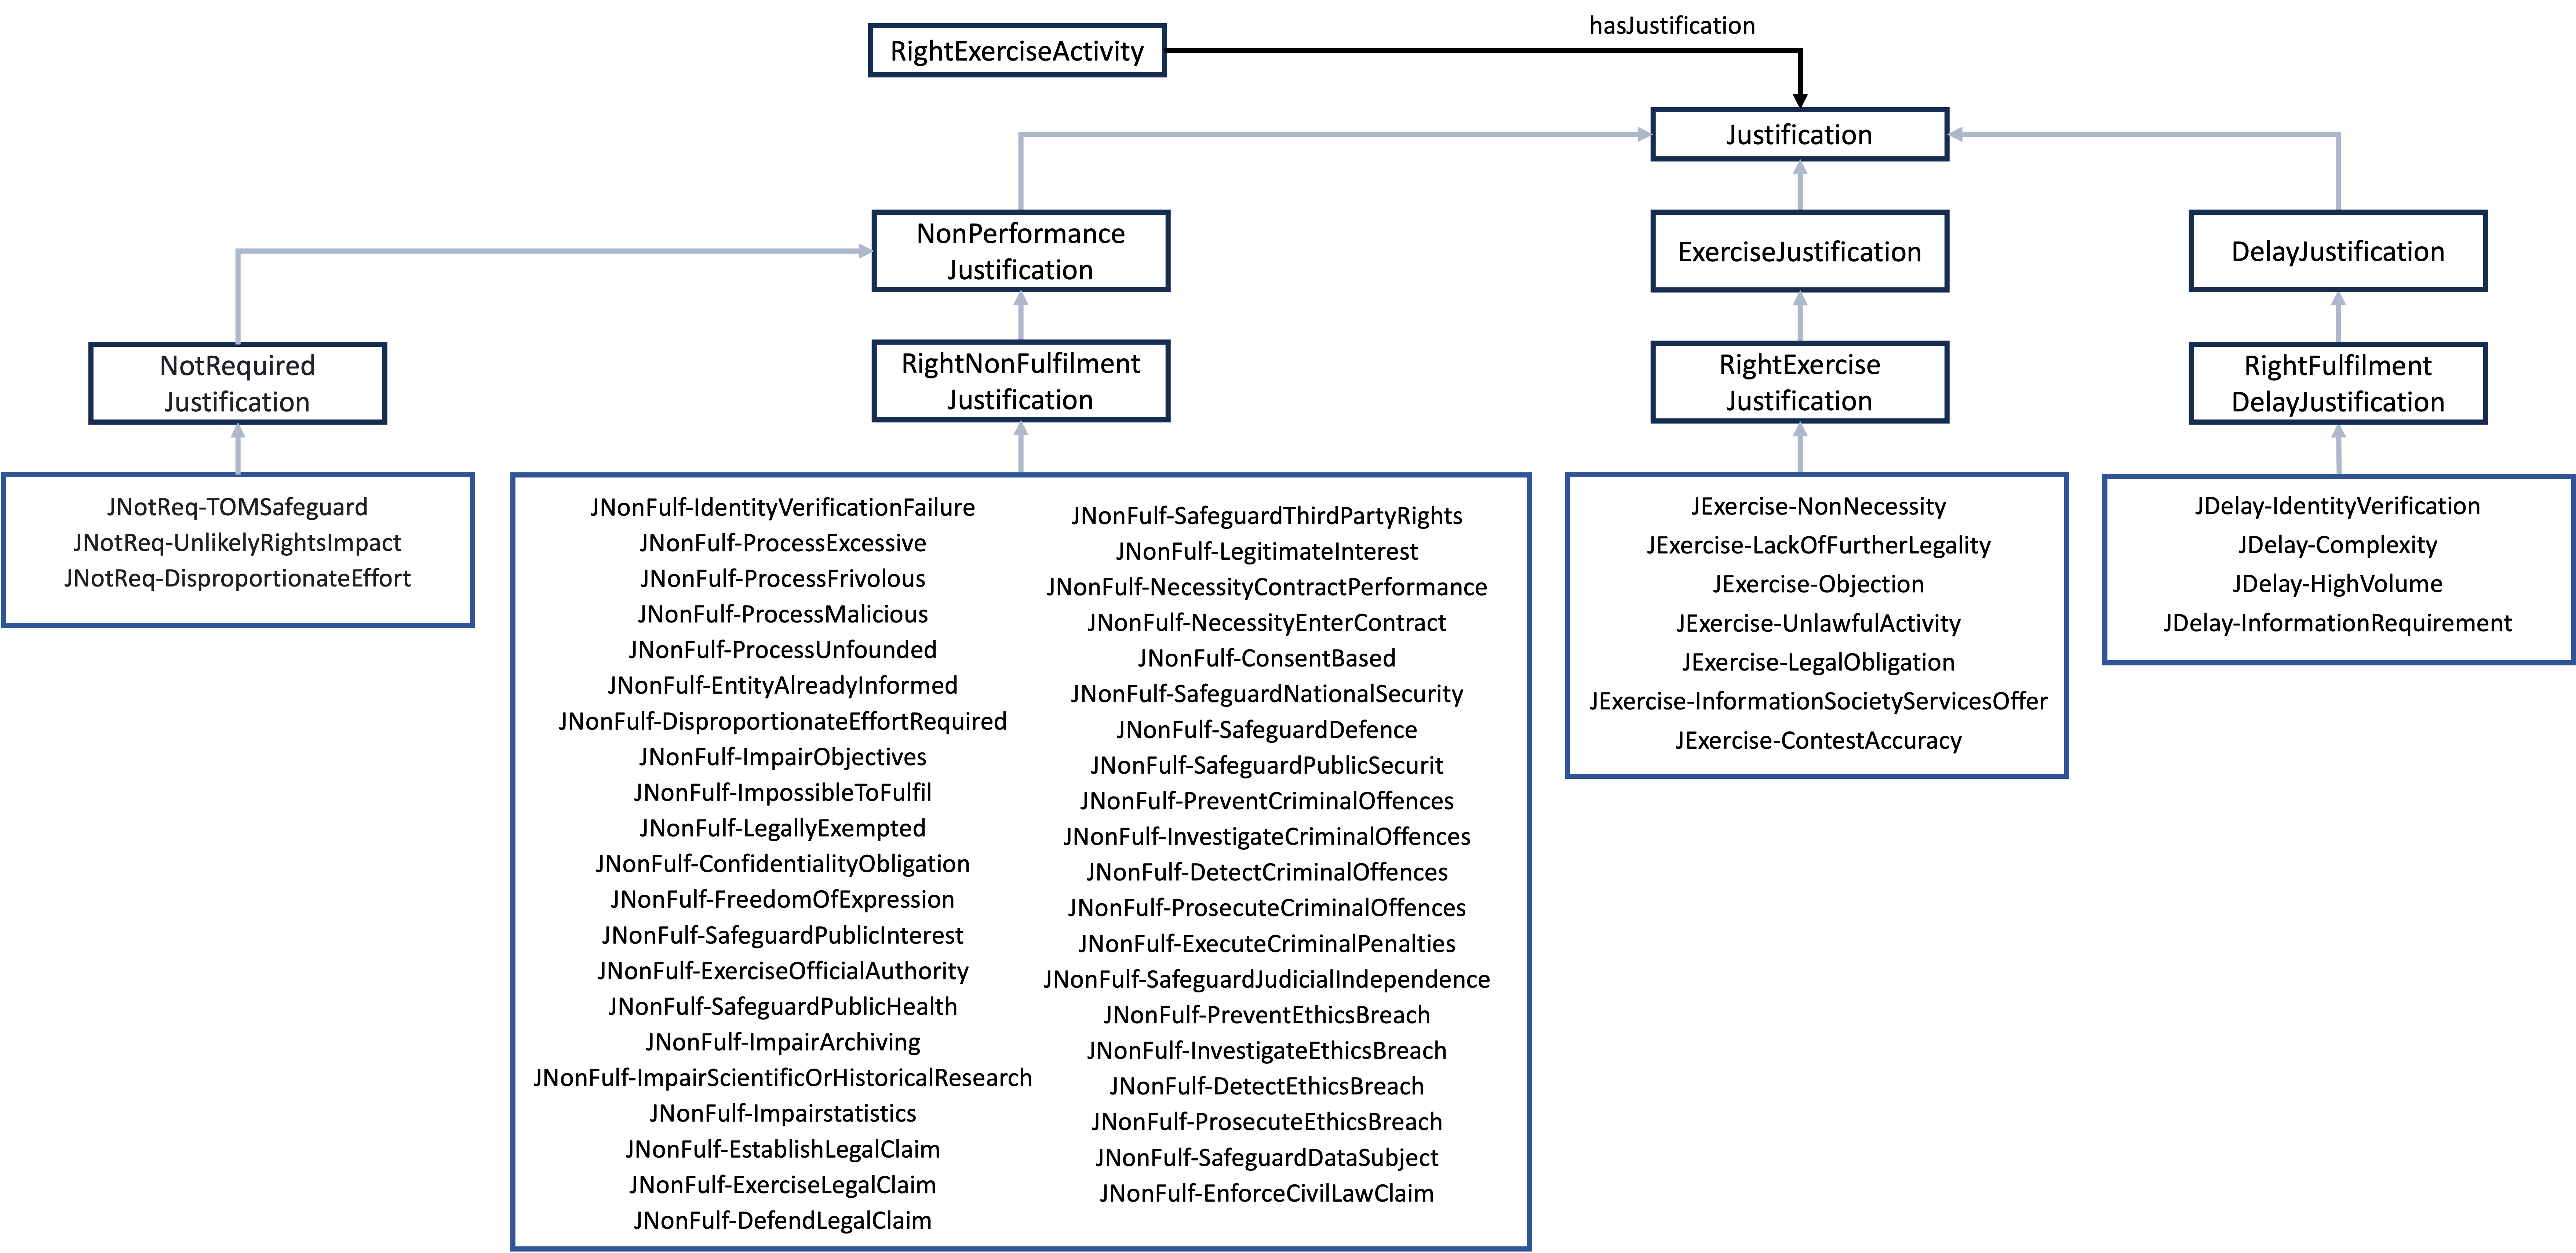
\includegraphics[width=\linewidth]{figures/chapter-4/justifications.png}
    \caption[Justification concepts.]{Justification concepts for the non-fulfilment, delay of fulfilment and exercise of rights.}
    \label{fig:justifications}
\end{figure}

Additionally, to track the status of rights exercising activities, a set of request statuses are modelled in DPV, including \texttt{RequestAccepted} for a request being accepted towards fulfilment, \texttt{RequestRejected} for a request being rejected towards non-fulfilment or\linebreak \texttt{RequestRequiresAction} for a request requiring an action to be performed from another party, and the \texttt{isBefore} and \texttt{isAfter} concepts can be used to specify that a specific activity occurs before or after another activity.

While this modelling was inspired by the GDPR, the concepts are described in a jurisdiction-agnostic manner so that they can be used to tackle data protection regulations in different jurisdictions.
For GDPR-specific rights, the \texttt{DataSubjectRight} concept is extended in DPV-GDPR with the data subject rights described in GDPR's Articles 13 to 22, as well as the rights to withdraw consent and to lodge a complaint with a supervisory authority, described in Articles 7.3 and 77.
Moreover, notices for direct and indirect data collection, to fulfil the information requirements in Articles 13 and 14, for Subject Access Requests (SARs), described in Article 15, and for notifying recipients, necessary to fulfil the communication requirements of Articles 16, 17 and 18, are provided as GDPR-specific subclasses of \texttt{RightFulfilmentNotice}s.

An overview of the aforementioned requirements and the intended purpose for modelling these concepts is presented in the ORSD illustrated in Table~\ref{tab:rights_ORSD}.

% also with these questions(in the ORSD) can you link directly to gdpr articles or other literature of gdpr implementation that help indicate these are valid requirements?

\begin{table}[htbp]
\centering
\caption{ORSD of the proposed model to express rights-related activities.}
\label{tab:rights_ORSD}
\scriptsize
\resizebox{\textwidth}{!}{%
\begin{tabular}{| l | l | l | l  | l | l | l |l| }
\hline
\multicolumn{8}{|c|}{\cellcolor[HTML]{A0A0A0}\textbf{Vocabulary-based patterns for rights exercising activities}} \\ \hline
\multicolumn{8}{|c|}{\cellcolor[HTML]{EFEFEF}\textbf{1. Purpose}} \\ \hline
\multicolumn{8}{| p{12.0cm} |}{The purpose of this model is the expression of rights-related activities, in particular focusing on data subject rights, such as the ones described in GDPR's Chapter III.} \\ \hline
\multicolumn{8}{|c|}{\cellcolor[HTML]{EFEFEF}\textbf{2. Scope}} \\ \hline
\multicolumn{8}{| p{12.0cm} |}{The scope of this model is limited to the expression of information related to the various steps of exercising data subject rights. In particular, the introduced concepts serve one of these purposes: (i) indicate what rights exist, (ii) express where such rights can be exercised, and (iii) record information related to concrete instances of rights that are being or were exercised. } \\ \hline
\multicolumn{8}{|c|}{\cellcolor[HTML]{EFEFEF}\textbf{3. Implementation Language}} \\ \hline
\multicolumn{8}{| p{12.0cm} |}{RDF, RDFS} \\ \hline
\multicolumn{8}{|c|}{\cellcolor[HTML]{EFEFEF}\textbf{4. Intended End-Users}} \\ \hline
\multicolumn{8}{| p{12.0cm} |}{Developers of Web services and applications, including decentralised storage solutions, that handle personal data.} \\ \hline
\multicolumn{8}{|c|}{\cellcolor[HTML]{EFEFEF}\textbf{5. Intended Uses}} \\ \hline
\multicolumn{8}{| p{12.0cm} |}{
Use 1. Declaration of the existence of data subject rights when the usage and collection of personal data is performed by Web services providers and developers, including information on where they can be exercised. \newline
Use 2. Patterns for data subject rights that can be fulfilled. \newline
Use 3. Patterns for data subject rights that cannot be fulfilled, including justifications for non-fulfilment. \newline
Use 4. Fulfilment of data subject rights requests from specific data protection legislation, such as the GDPR.
 } \\ \hline
\multicolumn{8}{|c|}{\cellcolor[HTML]{EFEFEF}\textbf{6. Ontology Requirements}} \\ \hline
\multicolumn{8}{|c|}{\cellcolor[HTML]{EFEFEF}\textbf{a. Non-Functional Requirements}}    \\ \hline
\multicolumn{8}{| p{12.0cm} |}{
NFR 1. The concepts are either published online within DPVCG's outputs, following W3C's specification format, or are under discussion for being adopted by the same CG. } \\ \hline
\multicolumn{8}{|c|}{\cellcolor[HTML]{EFEFEF}\textbf{b. Functional  Requirements: Groups of Competency Questions}}  \\ \hline
\multicolumn{5}{|c|}{\cellcolor[HTML]{EFEFEF}CQRG1. Related to data subject rights} & \multicolumn{3}{|c|}{\cellcolor[HTML]{EFEFEF}CQRG2. Related to GDPR} \\ \hline
\multicolumn{5}{ | m{7cm} |}{
CQR1. What rights are applicable in a given context? \newline
CQR2. Where can the right be exercised? \newline
CQR3. How can the right be exercised? \newline
CQR4. What data is necessary to implement the right? \newline 
CQR5. Which entity implements the right? \newline 
CQR6. Which entity exercised the right? \newline 
CQR7. When is the exercising activity occurring? \newline 
CQR8. What is the status of the right request? } & 
\multicolumn{3}{ m{5cm} |}{
CQR9. Which data subject rights are applicable according to the legal basis used by the data controller? \newline
CQR10. Which provenance metadata must controllers provide when replying to data subject rights requests? \newline 
CQR11. Which justification can be provided to not fulfil, delay or exercise a request?
}\\ \hline
\end{tabular}}
\vspace{-0.1in}
\end{table}

\subsection{Vocabulary-based patterns for rights exercising activities}
\label{sec:rights_patterns}

This Section outlines the usage of DPV for the expression of rights exercising activities, specifically related to the data subject rights described in GDPR's Chapter III.
Accordingly, the \textit{``controller shall take appropriate measures to provide any information referred to in Articles 13 and 14 and any communication under Articles 15 to 22 [...] to the data subject in a concise, transparent, intelligible and easily accessible form''} and if \textit{``the data subject makes the request by electronic form means, the information shall be provided by electronic means where possible, unless otherwise requested by the data subject''} \citeyearpar{noauthor_regulation_2016}.
Consequently, in this Thesis, personal data processing-related vocabularies such as DPV, and other semantic metadata vocabularies such as DCMI Metadata Terms and DCAT, are used for the establishment of structured notices and records of activities, which promote the fulfilment of the transparency and machine-readability requirements previously described.
Additionally, by storing such information in decentralised personal datastores, the accessibility requirement can also be satisfied.

Listing~\ref{list:applicable_rights} provides an example of a personal data handling activity, which can be used to express information regarding the what, how, where, who, and why personal data is being processed, as well as what rights exist.
The example provides information regarding the type of personal data, \texttt{pd:EmailAddress}, being processed by the \texttt{ex:DataController}, the purpose and legal basis used for the processing to occur, \texttt{dpv:ServiceProvision} and \texttt{eu-gdpr:A6-1-a}, and the applicable GDPR data subject rights.
This pattern can be followed by data controllers to express which rights are applicable, including rights beyond the ones in the GDPR, e.g., EU's fundamental rights and the rights depicted in other EU regulations or in other jurisdictions.

\begin{listing}[htp]
\caption[Personal data handling activity with applicable rights.]{Personal data handling activity example which includes information regarding the applicable rights.}
\label{list:applicable_rights}
\begin{minted}{turtle}
ex:ProcessEmailForServiceProvision a dpv:PersonalDataHandling ;
    dpv:hasDataController ex:DataController ;
    dpv:hasPersonalData pd:EmailAddress ;
    dpv:hasProcessing dpv:Collect, dpv:Use ;
    dpv:hasPurpose dpv:ServiceProvision ;
    dpv:hasLegalBasis eu-gdpr:A6-1-a ;
    dpv:hasRight eu-gdpr:A7-3, eu-gdpr:A13, eu-gdpr:A14, eu-gdpr:A15, eu-gdpr:A16, eu-gdpr:A17, eu-gdpr:A18, eu-gdpr:A20, eu-gdpr:A22, eu-gdpr:A77 .
ex:DataController a dpv:DataController .
\end{minted}
\end{listing}

Moreover, such declarations of applicable rights should include a notice of where they can be exercised.
Thus, as described in the previous Section, DPV’s \texttt{isExercisedAt} property should be used to connect rights with information on where to exercise it.
Such information should be provided through a \texttt{RightExerciseNotice}, along with other rights exercising metadata.

Listing~\ref{list:exercise_point} provides a notice with information on where to exercise the GDPR's right of access related to personal data being processed by the \texttt{ex:DataController}.
This notice uses the \texttt{dpv:hasRight} property to indicate which rights can be exercised, beyond the already mentioned access right, and the \texttt{foaf:page} property to express the precise Web page where the right can be exercised.
Additionally, DPV's \texttt{hasDataController} and\linebreak \texttt{isImplementedByEntity} properties are used to define who is the controller responsible for the personal data being processed and who is the entity implementing the service/platform where the rights are exercised -- in most cases this entity will probably coincide with the data controller, however, for transparency and accountability purposes, it is reasonable to express both terms.
Other entity-related properties can also be used to personalise the notice, e.g., if a notice is personalised for a specific data subject, then \texttt{dpv:hasDataSubject} can be used to connect the notice with the individual data subject. 
Furthermore, personal data handling instances can also be used to express `data processing bundles' that need to be provided in order to fulfil the data subjects' rights.
As previously mentioned, this can be done using DPV's taxonomies of purposes, personal data categories, processing operations, etc, e.g., in Listing~\ref{list:exercise_point}, an account identifier is required by the data controller for identity verification purposes in order to fulfil the data subject's rights described in GDPR's Articles 7.3, 15, 16, 17 and 20.
Other information might be needed to be communicated to the user, for instance, information on payments as Article 12.5(a) states that a fee \textit{``taking into account the administrative costs of providing the information or communication or taking the action requested''} might be requested by the data controller in case the data subject's request is unfounded, excessive or repetitive.
Such information can also be expressed in personal data handling instances including ODRL policies with duties constrained with an \texttt{odrl:payAmount} left operand.
% need to be provided / are being provided

\begin{listing}[htp]
\caption[GDPR Article 15's right of access exercise notice.]{GDPR Article 15's right of access exercise notice, including information on where to exercise the right and on necessary data to fulfil the right.}
\label{list:exercise_point}
\begin{minted}{turtle}
ex:RightToAccess a eu-gdpr:A15 ;
    dpv:isExercisedAt ex:RightExercisePoint .

ex:RightExercisePoint a dpv:RightExerciseNotice ;
    dpv:hasRight eu-gdpr:A7-3, eu-gdpr:A15, eu-gdpr:A16, eu-gdpr:A17, eu-gdpr:A20 ;
    dpv:hasDataController ex:DataController ;
    dpv:isImplementedByEntity ex:DataController ;
    foaf:page <https://example.com/DataController/RightExercisePoint> ;
    dpv:hasPersonalDataHandling [ 
        a dpv:PersonalDataHandling ;
        dpv:hasPurpose dpv:IdentityVerification ;
        dpv:hasPersonalData pd:AccountIdentifier ;
        dpv:hasProcessing dpv:Collect, dpv:Store ;
        dpv:hasRecipientDataController ex:DataController ] .
\end{minted}
\end{listing}

In addition to notices expressing what rights are applicable and where they can be exercised, provenance metadata must be kept when actual instances of the rights are exercised, throughout the whole process, from initiating a request to rejecting or fulfilling it.
As such, DPV's \texttt{RightExerciseActivity} can be used in conjunction with the W3C's PROV-O recommendation~\citep{lebo_prov-o_2013} to track the provenance of a right exercising activity instance.
Using this standard, provenance information, regarding the entities whom the request is associated with, i.e., \texttt{prov:wasAssociatedWith}, or what data/notice was generated, i.e., \texttt{prov:generated}, by the right exercise activity, can be represented.
\texttt{prov:actedOnBehalfOf} can also be used to represent delegation or representation, for instance when a parent exercises a right on behalf of its child.
Temporal information, descriptions and identifiers of the activities and their creators/publishers can be recorded using DCMI Metadata Terms.
Connections to the previous or following activities can be done using the \texttt{dpv:isAfter} and \texttt{dpv:isBefore} concepts, respectively.
Moreover, to track the status of a right exercising activity, DPV's taxonomy of request statuses concepts can be used.

Figure~\ref{fig:request_status} illustrates the sequence in which these concepts occur.
Once the request is initiated, it should be then acknowledged by the entity implementing it and either accepted towards fulfilment or rejected towards non-fulfilment.
Additionally, after being rejected, the entity fulfilling the request can also require further action from the requester (e.g., request additional data to be able to fulfil the request), which can delay the acceptance or rejection of the request, and after the required action is performed, the request can either be accepted towards fulfilment or get rejected again towards non-fulfilment or towards asking again for further action.

% perhaps formalise the semantics a bit more using uml state machine notation?
\begin{figure}[htp]
    \centering
    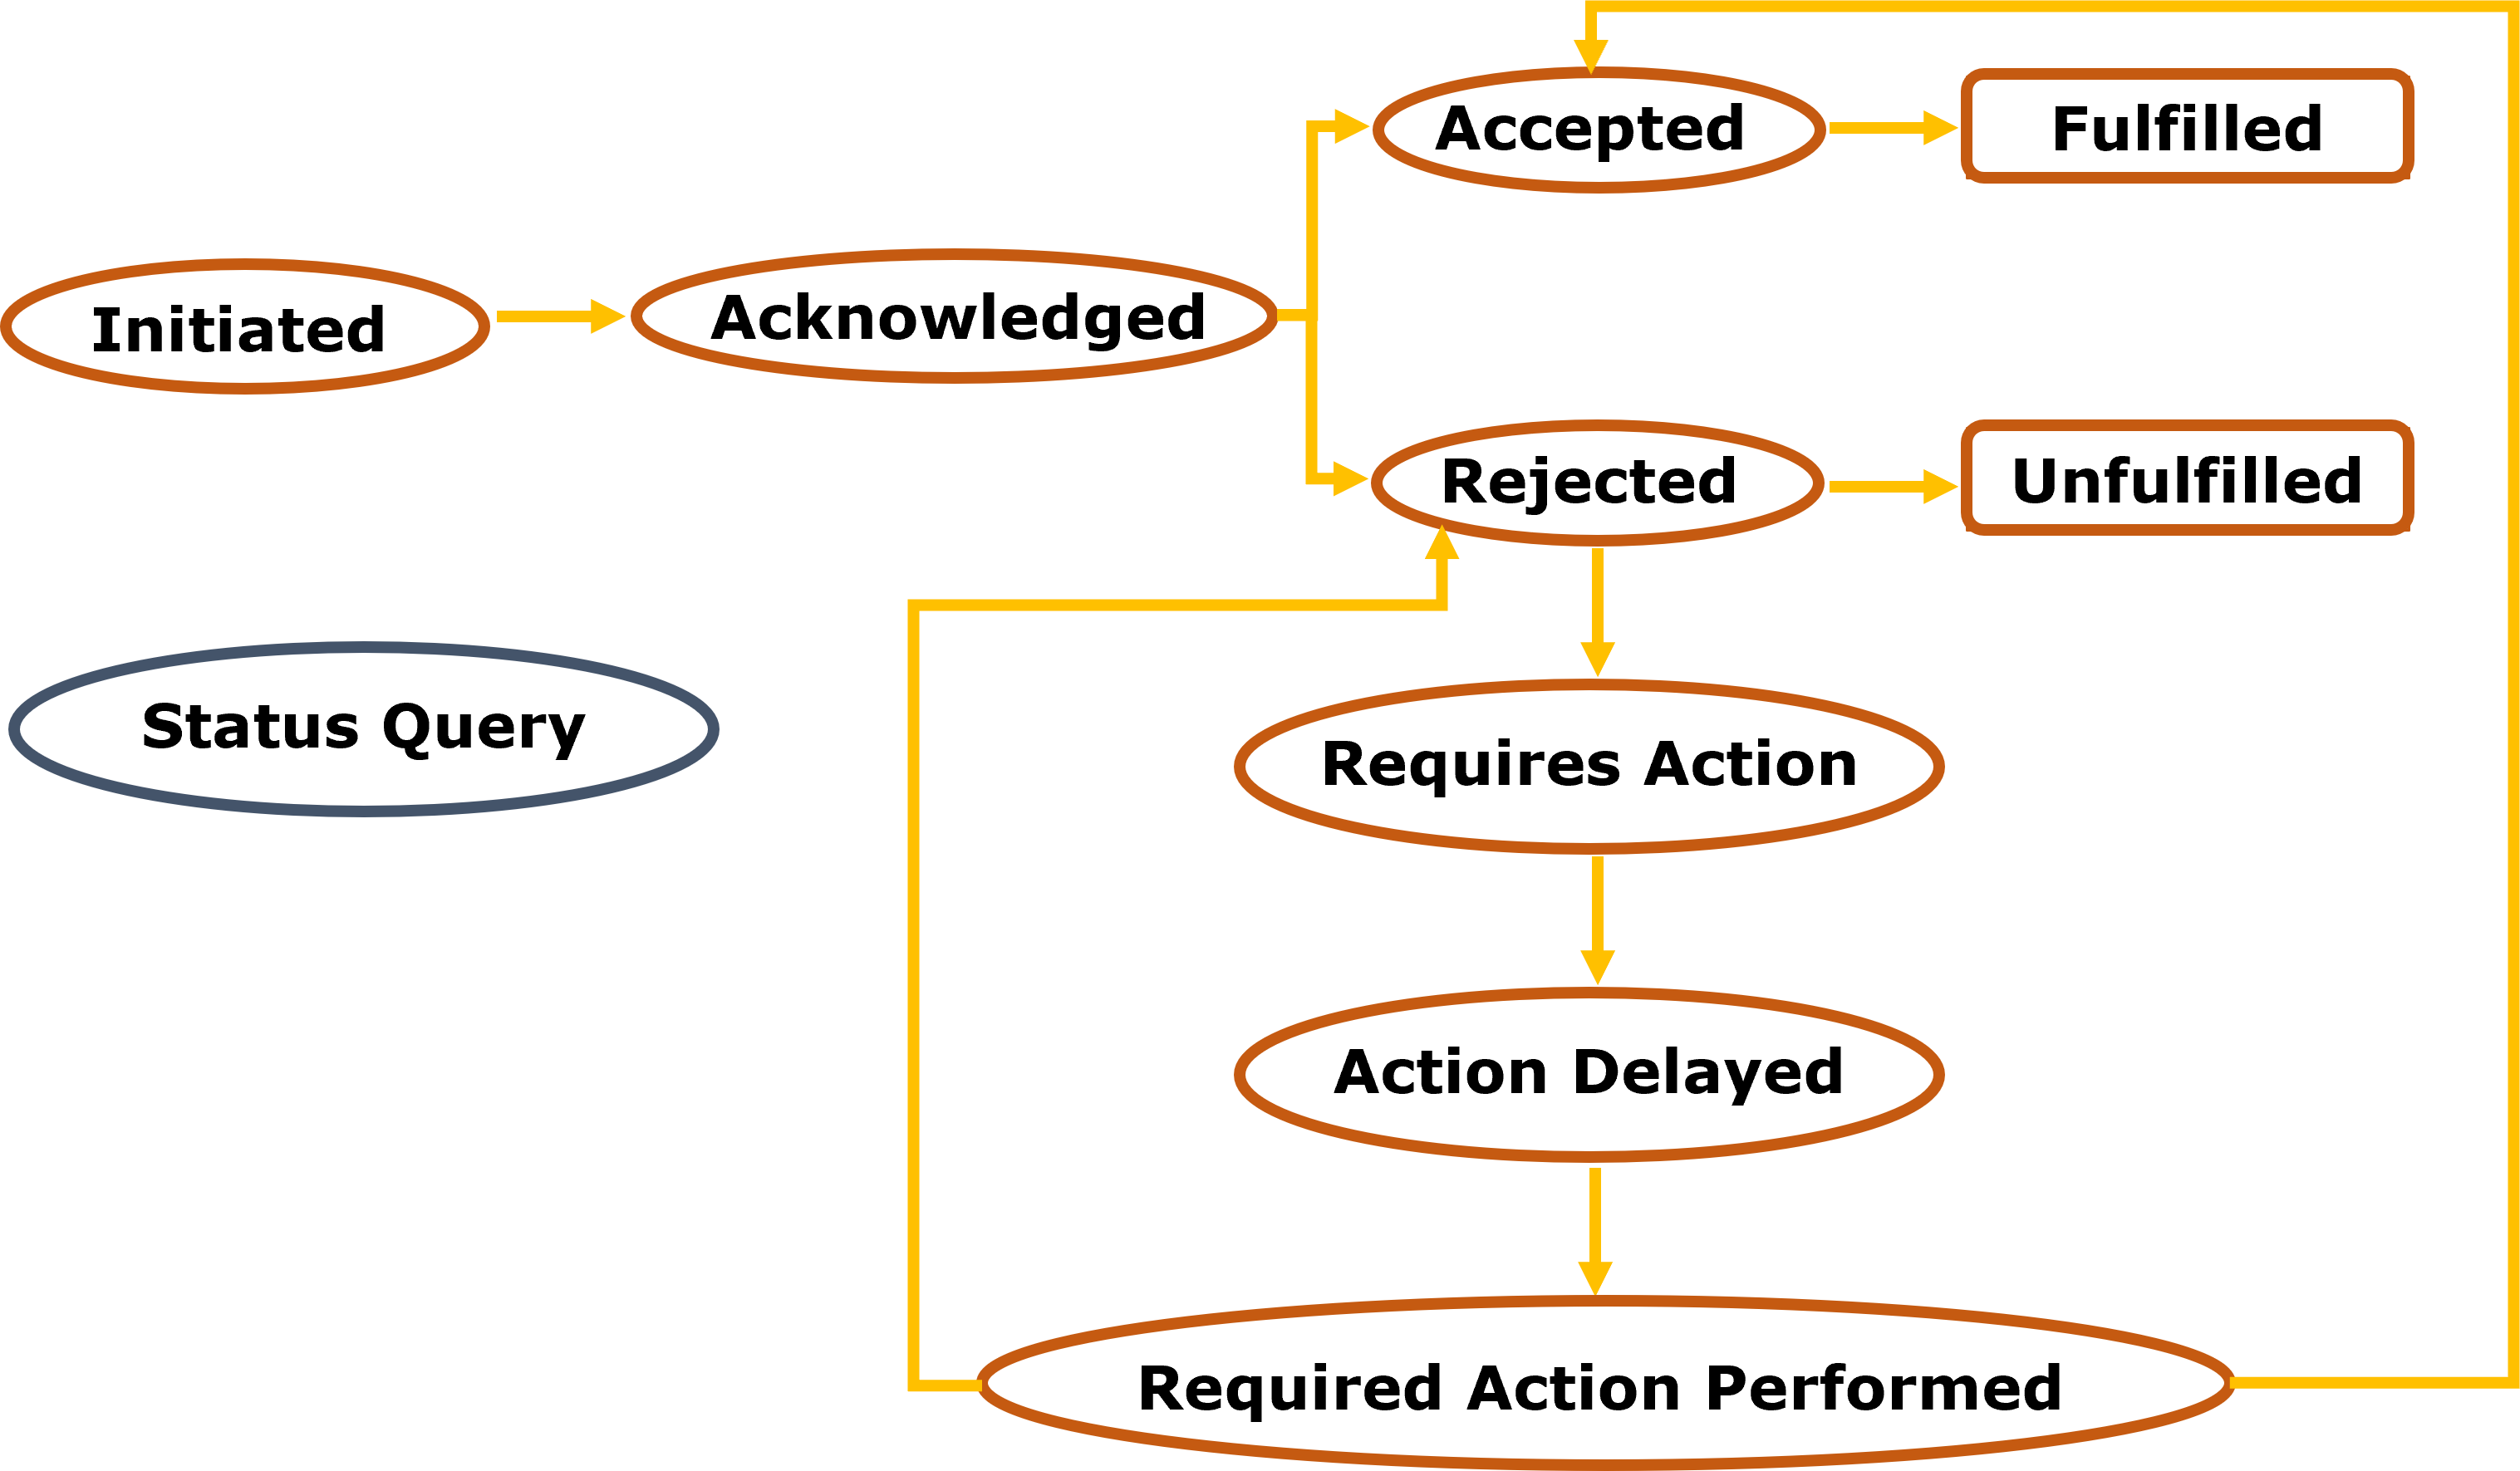
\includegraphics[width=0.8\linewidth]{figures/chapter-4/request-status.png}
    \caption{DPV's concepts to model the status of a request.}
    \label{fig:request_status}
\end{figure}

Listing~\ref{list:request_acknowledgment} illustrates a record of the right exercising activities related to a GDPR right of access request and acknowledgement of said request.
The activity associated with the start of the request has the status \texttt{dpv:RequestInitiated}, the data subject is identified using the \texttt{dpv:hasDataSubject} and the recipient of the request, a data controller, using the \texttt{dpv:hasRecipientDataController}.
Furthermore, a personal data handling instance can be used to express what personal data needs to be processed for the fulfilment of the right and DPV's \texttt{hasScope} to specify the scope of the request, e.g., the data subject only wants to access data processed for service provision purposes or only data processed during 2022.
Following the start of the request, the controller acknowledges the request, a right exercising activity which has \texttt{dpv:RequestAcknowledged} status and the recipient is the data subject that initiated the request.

\begin{listing}[htp]
\caption{Record of GDPR right of access request and acknowledgement activities.}
\label{list:request_acknowledgment}
\begin{minted}{turtle}
ex:DataSubject a dpv:DataSubject .
ex:DataSubjectUsername a pd:AccountIdentifier ;
    dpv:hasDataSubject ex:DataSubject .

ex:SARequest a dpv:RightExerciseActivity, prov:Activity ;
    dcterms:description "Data Subject makes a GDPR right of access request" ;
    dpv:hasRight eu-gdpr:A15 ;
    dpv:isExercisedAt ex:RightExercisePoint ;
    prov:wasAssociatedWith ex:DataSubject ;
    dpv:hasDataSubject ex:DataSubject ;
    dpv:hasRecipientDataController ex:DataController ;
    dcterms:date "2023-11-02T11:08:05"^^xsd:dateTime ;
    dpv:hasStatus dpv:RequestInitiated ;
    dpv:hasPersonalDataHandling [
        a dpv:PersonalDataHandling ;
        dpv:hasPurpose dpv:IdentityVerification ;
        dpv:hasPersonalData ex:DataSubjectUsername ;
        dpv:hasProcessing dpv:Collect, dpv:Store ] ;
    dpv:hasScope [
        dpv:hasPurpose dpv:ServiceProvision ;
        dpv:hasDuration [
            time:hasBeginning "2022-01-01T00:00:00"^^xsd:dateTime ;
            time:hasEnd "2022-12-31T23:59:59"^^xsd:dateTime ] ] .

ex:SARAcknowledged a dpv:RightExerciseActivity, prov:Activity ;
    dcterms:description "Data controller acknowledges the request" ;
    dcterms:date "2023-11-02T15:55:10"^^xsd:dateTime ;
    prov:wasAssociatedWith ex:DataController ;
    dpv:hasRecipient ex:DataSubjectUsername ;
    dpv:hasStatus dpv:RequestAcknowledged ;
    dpv:isAfter ex:SARequest .
\end{minted}
\end{listing}

Listing~\ref{list:further_action} illustrates the follow-up to Listing~\ref{list:request_acknowledgment} -- the request was rejected\linebreak due to the data controller not being able to identify the data subject,\linebreak \texttt{JNonFulf-IdentityVerificationFailure}.
Table~\ref{tab:justifications} contains the list of modelled right non-fulfilment justifications and their labels, which can be used by controllers for the purpose of justifying such requests.
As such the data controller requires further information from the data subject to be able to proceed with the request.
Such right exercise activity is identified with the \texttt{dpv:RequestRequiresAction} status and contains a personal data handling activity instance expressing the information that the data subject needs to provide for the right exercise to continue.
Afterwards, a right exercise activity associated with the data subject and with a \texttt{dpv:RequestRequiredActionPerformed} status is recorded with the information that the data subject provided.

\begin{listing}[htp]
\caption[Record requesting further information to fulfil SAR.]{Record of data controller requesting further information to fulfil the data subject's SAR and of the data subject providing the controller with said information.}
\label{list:further_action}
\begin{minted}{turtle}
ex:SARRejected a dpv:RightExerciseActivity, prov:Activity;
    dcterms:description "Data controller rejects the request" ;
    dcterms:date "2023-11-02T15:57:31"^^xsd:dateTime ;
    prov:wasAssociatedWith ex:DataController ;
    dpv:hasRecipient ex:DataSubjectUsername ;
    dpv:hasStatus dpv:RequestRejected ;
    dpv:hasJustification justif:JNonFulf-IdentityVerificationFailure ;
    dpv:isAfter ex:SARAcknowledged .

ex:SARRequiresAction a dpv:RightExerciseActivity, prov:Activity ;
    dcterms:description "Data controller requires further actions" ;
    dcterms:date "2023-11-02T16:09:21"^^xsd:dateTime ;
    prov:wasAssociatedWith ex:DataController ;
    dpv:hasRecipient ex:DataSubjectUsername ;
    dpv:hasStatus dpv:RequestRequiresAction ;
    dpv:hasJustification justif:JNonFulf-IdentityVerificationFailure ;
    dpv:hasPersonalDataHandling [
        dpv:hasPersonalData pd:OfficialID ;
        dpv:hasProcessing dpv:MakeAvailable ;
        dpv:hasPurpose dpv:IdentityVerification ;
        dpv:hasRecipientDataController ex:DataController ;
        dpv:isImplementedByEntity ex:DataSubjectUsername ] ;
    dpv:isAfter ex:SARRejected .

ex:DataSubjectOfficialID a pd:OfficialID ;
    dpv:hasDataSubject ex:DataSubject .

ex:SARActionPerformed a dpv:RightExerciseActivity, prov:Activity ;
    dcterms:description "Data Subject provides required information" ;
    dcterms:date "2023-11-02T17:20:42"^^xsd:dateTime ;
    prov:wasAssociatedWith ex:DataSubject ;
    dpv:hasStatus dpv:RequestRequiredActionPerformed ;
    dpv:hasPersonalDataHandling [
        dpv:hasPersonalData ex:DataSubjectOfficialID ;
        dpv:hasProcessing dpv:MakeAvailable ;
        dpv:hasPurpose dpv:IdentityVerification ;
        dpv:hasRecipientDataController ex:DataController ;
        dpv:isImplementedByEntity ex:DataSubjectUsername ] ;
    dpv:isAfter ex:SARRequiresAction .
\end{minted}
\end{listing}

% rights non-fulfilment justifications issue: https://github.com/w3c/dpv/issues/63 & meeting minutes:https://www.w3.org/2022/10/19-dpvcg-minutes.html
\begin{landscape}
\begin{table}
    \centering
    \caption{Justifications for non-fulfilment of GDPR's data subject rights.}
    \label{tab:justifications}
    \resizebox{\textwidth}{!}{%
    \begin{tabular}{c|l|c}
        \textbf{Term} & \textbf{Label} & \multicolumn{1}{c}{\begin{tabular}[c]{@{}c@{}} \textbf{GDPR} \\ \textbf{Article(s)} \end{tabular}} \\
        \hline\hline
        \texttt{JNonFulf-IdentityVerificationFailure} & \multicolumn{1}{l|}{\begin{tabular}[l]{@{}l@{}} Justification that the process could not be fulfilled or was not successful\\ because identity verification failed \end{tabular}} & 12.2 \\
        \hline
        \texttt{JNonFulf-ProcessExcessive} & Request was excessive in scope & 12.5 \\
        \hline
        \texttt{JNonFulf-ProcessFrivolous} & Request was frivolous in scope & 12.5 \\
        \hline
        \texttt{JNonFulf-ProcessMalicious} & Request was malicious in scope & 12.5 \\
        \hline
        \texttt{JNonFulf-ProcessUnfounded} & Request was unfounded in scope & 12.5 \\
         \hline
        \texttt{JNonFulf-EntityAlreadyInformed} & \multicolumn{1}{l|}{\begin{tabular}[l]{@{}l@{}} Data subject already has been provided with this information \end{tabular}} & 13.4, 14.5(a) \\
         \hline
        \texttt{JNonFulf-ImpairObjectives} & Fulfilment would cause impairment to processing & 14.5(b) \\
        \hline     
        \texttt{JNonFulf-DisproportionateEffortRequired} & Fulfilment would require extraordinary effort & 14.5(b), 19 \\
         \hline
        \texttt{JNonFulf-ImpossibleToFulfil} & Fulfilment would be impossible & 14.5(b), 19 \\
         \hline
        \texttt{JNonFulf-LegallyExempted} & \multicolumn{1}{l|}{\begin{tabular}[l]{@{}l@{}} Fulfilment not needed as it falls under legal exemption \end{tabular}} & \multicolumn{1}{l}{\begin{tabular}[l]{@{}l@{}} 14.5(c), 17.3(b),\\ 22.2(b) \end{tabular}} \\
         \hline
        \texttt{JNonFulf-ConfidentialityObligation} & \multicolumn{1}{l|}{\begin{tabular}[l]{@{}l@{}} Fulfilment would compromise existing confidentiality obligations \end{tabular}} & 14.5(d) \\
        \hline
        \texttt{JNonFulf-FreedomOfExpression} & \multicolumn{1}{l|}{\begin{tabular}[l]{@{}l@{}} Fulfilment would interfere with the right of freedom of expression\\ and information of others \end{tabular}} & 17.3(a) \\
         \hline
        \texttt{JNonFulf-SafeguardPublicInterest} & \multicolumn{1}{l|}{\begin{tabular}[l]{@{}l@{}} Fulfilment would interfere with necessary tasks carried out for public\\ interest \end{tabular}} & \multicolumn{1}{l}{\begin{tabular}[l]{@{}l@{}} 17.3(b), 21.6,\\ 23.1(e) \end{tabular}} \\
         \hline
         \texttt{JNonFulf-ExerciseOfficialAuthority} & \multicolumn{1}{l|}{\begin{tabular}[l]{@{}l@{}} Fulfilment would interfere with the exercise of official authorities \end{tabular}} & \multicolumn{1}{l}{\begin{tabular}[l]{@{}l@{}} 17.3(b), 20.3,\\ 23.1(h) \end{tabular}} \\
         \hline
         \texttt{JNonFulf-SafeguardPublicHealth} & \multicolumn{1}{l|}{\begin{tabular}[l]{@{}l@{}} Fulfilment would interfere with necessary tasks carried out for public\\ health reasons \end{tabular}} & 17.3(c) \\
         \hline
        \texttt{JNonFulf-ImpairArchiving} & \multicolumn{1}{l|}{\begin{tabular}[l]{@{}l@{}} Fulfilment would compromise or hinder archiving purposes \end{tabular}} & 17.3(d) \\
        \hline
        \texttt{JNonFulf-ImpairScientificOrHistoricalResearch} & \multicolumn{1}{l|}{\begin{tabular}[l]{@{}l@{}} Fulfilment would impair scientific or historical research \end{tabular}} & 17.3(d) \\
        \hline
        \texttt{JNonFulf-ImpairStatistics} & \multicolumn{1}{l|}{\begin{tabular}[l]{@{}l@{}} Fulfilment would interfere with official statistics \end{tabular}} & 17.3(d) \\
        \hline
        \texttt{JNonFulf-EstablishLegalClaim} & \multicolumn{1}{l|}{\begin{tabular}[l]{@{}l@{}} Fulfilment would interfere with the establishment of legal claims \end{tabular}} & 17.3(e), 21.1 \\
        \hline
        \texttt{JNonFulf-ExerciseLegalClaim} & \multicolumn{1}{l|}{\begin{tabular}[l]{@{}l@{}} Fulfilment would interfere with the exercise of legal claims \end{tabular}} & 17.3(e), 21.1 \\
        \hline
        \texttt{JNonFulf-DefendLegalClaim} & \multicolumn{1}{l|}{\begin{tabular}[l]{@{}l@{}} Fulfilment would interfere with the defence of legal claims \end{tabular}} & 17.3(e), 21.1 \\
        \hline
        \texttt{JNonFulf-SafeguardThirdPartyRights} & \multicolumn{1}{l|}{\begin{tabular}[l]{@{}l@{}} Fulfilment would adversely affect the rights of other data subjects or third\\ parties \end{tabular}} & 20.4, 23.1(i) \\
         \hline
         \texttt{JNonFulf-LegitimateInterest} & \multicolumn{1}{l|}{\begin{tabular}[l]{@{}l@{}} Fulfilment would interfere with the legitimate interest of the controller\\ which overrides the interests or rights of the data subject \end{tabular}} & 21.1 \\
         \hline
        \texttt{JNonFulf-NecessityContractPerformance} & \multicolumn{1}{l|}{\begin{tabular}[l]{@{}l@{}} Fulfilment would interfere with the performance of a contract \end{tabular}} & 22.2(a) \\
         \hline
        \texttt{JNonFulf-NecessityEnterContract} & \multicolumn{1}{l|}{\begin{tabular}[l]{@{}l@{}} Fulfilment would interfere with the necessity of entering into a contract \end{tabular}} & 22.2(a) \\
         \hline
        \texttt{JNonFulf-ConsentBased} & \multicolumn{1}{l|}{\begin{tabular}[l]{@{}l@{}} Fulfilment not necessary as processing is based on explicit consent \end{tabular}} & 22.2(c) \\
        \hline
        \texttt{JNonFulf-SafeguardNationalSecurity} & \multicolumn{1}{l|}{\begin{tabular}[l]{@{}l@{}} Fulfilment would pose a threat to safeguard national security \end{tabular}} & 23.1(a) \\
         \hline
        \texttt{JNonFulf-SafeguardDefence} & Fulfilment would pose a threat to safeguard defence & 23.1(b) \\
         \hline
        \texttt{JNonFulf-SafeguardPublicSecurity} & \multicolumn{1}{l|}{\begin{tabular}[l]{@{}l@{}} Fulfilment would pose a threat to safeguard public security \end{tabular}} & 23.1(c) \\
         \hline
        \texttt{JNonFulf-PreventCriminalOffences} & \multicolumn{1}{l|}{\begin{tabular}[l]{@{}l@{}} Fulfilment would interfere with the prevention of criminal offences \end{tabular}} & 23.1(d) \\
        \hline
        \texttt{JNonFulf-InvestigateCriminalOffences} & \multicolumn{1}{l|}{\begin{tabular}[l]{@{}l@{}} Fulfilment would interfere with the investigation of criminal offences \end{tabular}} & 23.1(d) \\
        \hline
        \texttt{JNonFulf-DetectCriminalOffences} & \multicolumn{1}{l|}{\begin{tabular}[l]{@{}l@{}} Fulfilment would interfere with the detection of criminal offences \end{tabular}} & 23.1(d) \\
        \hline
        \texttt{JNonFulf-ProsecuteCriminalOffences} & \multicolumn{1}{l|}{\begin{tabular}[l]{@{}l@{}} Fulfilment would interfere with the prosecution of criminal offences \end{tabular}} & 23.1(d) \\
        \hline
        \texttt{JNonFulf-ExecuteCriminalPenalties} & \multicolumn{1}{l|}{\begin{tabular}[l]{@{}l@{}} Fulfilment would interfere with the execution of criminal penalties \end{tabular}} & 23.1(d) \\
        \hline
        \texttt{JNonFulf-SafeguardJudicialIndependence} & \multicolumn{1}{l|}{\begin{tabular}[l]{@{}l@{}} Fulfilment would pose a threat to safeguard judicial independence or\\ proceedings \end{tabular}} & 23.1(f) \\
        \hline
        \texttt{JNonFulf-PreventEthicsBreach} & \multicolumn{1}{l|}{\begin{tabular}[l]{@{}l@{}} Fulfilment would interfere with the prevention of breaches of ethics for\\ regulated professions \end{tabular}} & 23.1(g) \\
        \hline
        \texttt{JNonFulf-InvestigateEthicsBreach} & \multicolumn{1}{l|}{\begin{tabular}[l]{@{}l@{}} Fulfilment would interfere with the investigation of breaches of ethics for\\ regulated professions \end{tabular}} & 23.1(g) \\
        \hline
        \texttt{JNonFulf-DetectEthicsBreach} & \multicolumn{1}{l|}{\begin{tabular}[l]{@{}l@{}} Fulfilment would interfere with the detection of breaches of ethics for\\ regulated professions \end{tabular}} & 23.1(g) \\
        \hline
        \texttt{JNonFulf-ProsecuteEthicsBreach} & \multicolumn{1}{l|}{\begin{tabular}[l]{@{}l@{}} Fulfilment would interfere with the prosecution of breaches of ethics for\\ regulated professions \end{tabular}} & 23.1(g) \\
        \hline
        \texttt{JNonFulf-SafeguardDataSubject} & \multicolumn{1}{l|}{\begin{tabular}[l]{@{}l@{}} Fulfilment would interfere with the protection of the data subject \end{tabular}} & 23.1(i) \\
         \hline
        \texttt{JNonFulf-EnforceCivilLawClaim} & Fulfilment would interfere with the enforcement of civil law claims & 23.1(j) \\
    \end{tabular}}
\end{table}
\end{landscape}
% Information is legally exempt from disclosure	- Documents that have personal data of the data subject exempt from disclosure in court proceedings apply in relation to a Subject Access Request, this applies to both legal advice and litigation privilege

Listing~\ref{list:sar_notice} illustrates the follow-up to Listing~\ref{list:further_action} -- the request was accepted and fulfilled by the data controller and as such the data controller provides the data subject with a notice of the fulfilment of GDPR's Art.15, modelled as a \texttt{eu-gdpr:SARNotice}, and a copy of the data whose access was requested, modelled as a \texttt{dcat:Dataset}.
Beyond temporal information and providing the location of the notice, a personal data handling instance can be used to provide additional information to the data subject -- in the case of this SAR notice, the data subject is also notified of the type of personal data being processed, the purpose for the processing, the time period when the data was processed and the additional data subject rights that can be exercised.

\begin{listing}[htp]
\caption[Record of the acceptance and fulfilment of a SAR request.]{Record of the acceptance and fulfilment of the request and respective \texttt{SARNotice}.}
\label{list:sar_notice}
\begin{minted}{turtle}
ex:SARAccepted a dpv:RightExerciseActivity, prov:Activity ;
    dcterms:description "Request accepted by data controller towards fulfilment" ;
    dcterms:date "2023-11-03T08:15:04"^^xsd:dateTime ;
    prov:wasAssociatedWith ex:DataController ;
    dpv:hasRecipient ex:DataSubjectUsername ;
    dpv:hasStatus dpv:RequestAccepted ;
    dpv:isAfter ex:SARActionPerformed .

ex:SARFulfilled a dpv:RightExerciseActivity, prov:Activity ;
    dcterms:description "Request fulfilled by data controller" ;
    dcterms:date "2023-11-03T08:37:25"^^xsd:dateTime ;
    prov:wasAssociatedWith ex:DataController ;
    dpv:hasRecipient ex:DataSubjectUsername ;
    dpv:hasStatus dpv:RequestFulfilled ;
    prov:generated ex:DataCopy, ex:SARNotice_Username ;
    dpv:isAfter ex:SARAccepted .

ex:SARNotice_Username a eu-gdpr:SARNotice ;
    dcterms:date "2023-11-03T08:31:51"^^xsd:dateTime ;
    foaf:page <https://example.com/DataController/SARNotice_Username> ;
    dpv:hasPersonalDataHandling [
        dpv:hasPersonalData pd:EmailAddress ;
        dpv:hasPurpose dpv:ServiceProvision ;
        dpv:hasDuration [
            time:hasBeginning "2022-01-01T00:00:00"^^xsd:dateTime ;
            time:hasEnd "2022-12-31T23:59:59"^^xsd:dateTime ] ;
        dpv:hasRight eu-gdpr:A16, eu-gdpr:A17, eu-gdpr:A18, eu-gdpr:A21, eu-gdpr:A77 ] .

ex:DataCopy a dcat:Dataset ;
    dcterms:format <https://www.iana.org/assignments/media-types/text/csv> ;
    dcterms:accessRights access-right:c_16ec ; # restricted access
    dcterms:issued "2023-11-03T08:35:42"^^xsd:dateTime ;
    dcterms:valid "2023-12-03T08:35:42"^^xsd:dateTime ;
    dcat:landingPage <https://example.com/Username/SAR_DataCopy> .
\end{minted}
\end{listing}

Moreover, DCAT \citep{albertoni_data_2020} can be used to model resources beyond notices, for instance, a copy of the personal data, in the case of a right of access request according to the GDPR, as in Listing~\ref{list:sar_notice}.
Information regarding the format, validity and dataset provision/download location can be attached to the dataset representation using the \texttt{dcterms:format}, \texttt{dcterms:valid} and \texttt{dcat:landingPage} properties, respectively.
Additionally, DCAT -- and also the Data on the Web Best Practices Recommendation~\citep{loscio_data_2017} -- promotes the usage of ODRL to express license and rights statements, by linking the dataset with an ODRL policy using the \texttt{odrl:hasPolicy} property, or the usage of DCMI Metadata Terms' \texttt{license}, \texttt{accessRights} or \texttt{rights} properties to link datasets with licenses, access rights statements or other types of rights statements, e.g., copyrights, respectively.
In the case of using the latter, controlled vocabularies such as COAR's Access Rights vocabulary~\citep{apollaro_controlled_2022}, used in Listing~\ref{list:sar_notice} to restrict access only to the data subject, or the Named Authority List of Access rights from the~\cite{publications_office_of_the_european_union_named_2023} can be used to express `high-level' access control statements, e.g., embargoed, restricted or open access.
As such, by using DCAT and a policy expression vocabulary, i.e., ODRL, the user can easily control the transition of a compliance log and respective metadata, as proposed in PLASMA, from being only accessible by the user to be accessible by external auditors.

In this Section, the GDPR's Right of Access is used as an example to showcase how to model notices and right exercising activities using DPV, DCMI Metadata Terms, PROV-O and DCAT.
However, a similar pattern can be followed by data controllers to fulfil the other rights as in most cases the only substantial change would be the notice concept that needs to be used for a particular right instance, e.g., \texttt{eu-gdpr:DirectDataCollectionNotice} for the right fulfilment notice related to GDPR's Article 13, \texttt{eu-gdpr:IndirectDataCollectionNotice} for the right fulfilment notice related to GDPR's Article 14 or \texttt{eu-gdpr:RightsRecipientsNotice} for the right fulfilment notice related to GDPR's Article 19.
Moreover, some GDPR rights, such as the right to erasure in Article 17 and the right to restriction of processing in Article 18, also require the data subject to provide a justification for their request to be fulfilled by the data controller.
As such, a collection of justifications for the exercise of data subject rights, extracted from the GDPR and illustrated in Table~\ref{tab:fulfil_justifications}, was also modelled (as subclasses of a high-level \texttt{RightExerciseJustification} concept). % and is already approved to be integrated into DPV-GDPR's outputs.


\begin{table}
    \centering
    \caption[Justifications for the exercise of GDPR's data subject rights]{Justifications for the exercise of GDPR's data subject rights.}
    \label{tab:fulfil_justifications}
    \resizebox{\textwidth}{!}{%
    \begin{tabular}{c|p{8.5cm}|c}
        \textbf{Term} & \textbf{Label} & \multicolumn{1}{c}{\begin{tabular}[c]{@{}c@{}} \textbf{GDPR} \\ \textbf{Article(s)} \end{tabular}} \\
        \hline\hline
        \texttt{JExercise-NonNecessity} & \multicolumn{1}{l|}{\begin{tabular}[l]{@{}l@{}} Processing no longer necessary for the \\specified purposes \end{tabular}} & \multicolumn{1}{l}{\begin{tabular}[l]{@{}l@{}} 17.1(a),\\ 18.1(c) \end{tabular}} \\
        \hline
        \texttt{JExercise-LackOfFurtherLegality} & \multicolumn{1}{l|}{\begin{tabular}[l]{@{}l@{}} Processing no longer necessary due to a lack of further\\ legality of the legal basis of specified context \end{tabular}} & 17.1(b) \\
        \hline
        \texttt{JExercise-Objection} & Data subject objected to the processing & \multicolumn{1}{l}{\begin{tabular}[l]{@{}l@{}} 17.1(c),\\ 18.1(d) \end{tabular}} \\
        \hline
        \texttt{JExercise-UnlawfulActivity} & Personal data unlawfully processed & \multicolumn{1}{l}{\begin{tabular}[l]{@{}l@{}} 17.1(d),\\ 18.1(b) \end{tabular}} \\
        \hline
        \texttt{JExercise-LegalObligation} & Compliance with a legal obligation & 17.1(e) \\
        \hline
        \texttt{JExercise-InformationSocietyServicesOffer} & \multicolumn{1}{l|}{\begin{tabular}[l]{@{}l@{}} Personal data collected in relation to the offer \\of information society services \end{tabular}} & 17.1(f) \\
        \hline
        \texttt{JExercise-ContestAccuracy} & \multicolumn{1}{l|}{\begin{tabular}[l]{@{}l@{}} Accuracy of personal data contested by the \\data subject \end{tabular}} & 18.1(a) \\
    \end{tabular}}
\end{table}

\subsection{Justifications publication and maintenance}
\label{sec:justifications_publication}

As discussed in the previous sections, most rights-related concepts were already proposed and are integrated into DPV and DPV-GDPR.
The justifications concepts have already been approved to be accepted, but are still to be published in DPVCG's outputs.
As such, the justifications vocabulary human-readable documentation and machine-readable file are available at \url{https://w3id.org/people/besteves/justifications} using content negotiation.
Once the justification terms are fully integrated into DPV, this documentation will be archived as the maintenance of the terms will be performed as part of the DPVCG's activities.

The HTML documentation includes a description of the defined terms, which was conducted and validated with domain experts\footnote{This validation was performed with legal and ontology engineering experts in the context of W3C's DPV community group.}, diagrams with graphical representations of the several taxonomies used in the vocabulary patterns specific in this section, and RDF examples that use the defined terms to express rights-related activities.
The vocabulary documentation also includes metadata, such as the identity of the creators and publishers of the ontology, the dates of creation and last modification or the version number.
The source code is hosted at \url{https://w3id.org/people/besteves/justifications/repo}, under the CC-BY-4.0 license.
The repository can also be used by implementers to suggest new inclusions to the vocabulary and to report bugs through GitHub Issues.

Additionally, an auxiliary webpage, openly available at \url{https://w3id.org/people/besteves/rights}, provides guidelines and further examples on how to use DPV and the developed \texttt{Justification} terms to model the vocabulary-based patterns for rights-related activities defined in this Section.
The source code is hosted at \url{https://w3id.org/people/besteves/rights/repo}, under the CC-BY-4.0 license.
\section{Ontology quality evaluation}
\label{sec:evaluation}

This Section describes the results of the ontologies quality evaluation, including the detection of common pitfalls with OOPS!\footnote{The OOPS! tool is available at \url{https://oops.linkeddata.es/} (accessed on 14 June 2023).}~\citep{poveda-villalon_oops_2014}, alignment with FAIR principles with FOOPS!\footnote{The FOOPS! tool is available at \url{https://w3id.org/foops} (accessed on 30 November 2023).}~\citep{garijo_foops_2021} and validation of competency questions with SPARQL queries~\citep{harris_sparql_2013}.

In terms of quality evaluation, the OOPS! tool was used to evaluate PLASMA and OAC in order to detect common errors in ontology development, such as missing domain or range properties or missing human-readable annotations.
Both evaluations did not detect any critical (issues affecting the ontology consistency, reasoning, or applicability) or important (issues not critical for ontology functionality but that should be corrected) pitfalls.
Furthermore, FOOPS! was used to evaluate the alignment of the developed vocabularies with the FAIR (Findable, Accessible, Interoperable and Reusable) principles.
Additionally, the vocabularies that were reused in this Section, e.g., DPV, ODRL, or ActivityStreams, were also evaluated with FOOPS! for comparison.
Table~\ref{tab:foops_evaluation} presents the results of this evaluation.

\begin{table}[htp]
    \centering
    \caption{Evaluation of the alignment of the developed and reused vocabularies with FAIR principles using FOOPS!.}
    \label{tab:foops_evaluation}
    \resizebox{\textwidth}{!}{%
    \begin{tabular}{c||c|c|c|c|c}
        \textbf{Ontology} & \textbf{FOOPS! score} & \textbf{Findable} & \textbf{Accessible} & \textbf{Interoperable} & \textbf{Reusable} \\
        \hline\hline
        OAC & 91\% & 8/9 & 2/3 & 3/3 & 8.83/9 \\
        \hline
        PLASMA & 91\% & 8/9 & 2/3 & 3/3 & 8.83/9 \\
        \hline 
        DPV & 64\% & 5.33/9 & 2/3 & 3/3 & 4.92/9 \\
        \hline 
        ODRL & 64\% & 4.5/9 & 3/3 & 3/3 & 4.75/9 \\
        \hline
        DCAT & 64\% & 4.33/9 & 3/3 & 3/3 & 5.14/9 \\
        \hline
        ACP & 52\% & 5.33/9 & 2/3 & 2/3 & 3.12/9 \\
        \hline
        ActivityStreams & 19\% & 2/9 & 1.5/3 & 0/3 & 1/9 \\
        \hline 
        ACL & 2\% & 0/9 & 0.5/3 & 0/3 & 0/9 \\
        \hline
        DCMI & 2\% & 0/9 & 0.5/3 & 0/3 & 0/9 \\
    \end{tabular}}
\end{table}

Both PLASMA and OAC obtained a good score in all FAIR aspects.
In terms of improvements, both vocabularies will be submitted to LOV (Linked Open Vocabularies), a public registry of ontologies that includes ontology metadata related to its terms and the creators/developers of the ontologies~\citep{dumontier_linked_2017}.
This will improve both the findability and the accessibility of the vocabularies.
Using Table~\ref{tab:foops_evaluation}, it can be observed that both PLASMA and OAC rate much higher than other reused ontologies in terms of findability and reusability as the used URIs and version URIs are persistent and resolvable, both include the recommended ontology and ontology terms metadata, a resolvable data usage license and provenance metadata.

Additionally, SPARQL queries are used to assess whether the developed models satisfy the competency questions, presented in Tables~\ref{tab:OAC_ORSD}, \ref{tab:plasma_orsd} and \ref{tab:rights_ORSD}, which were used to guide the development of the vocabularies in order to fulfil the identified requirements.

Table~\ref{tab:oac_cq_sparql} presents the SPARQL queries drafted to fulfil OAC's competency questions presented in Table~\ref{tab:OAC_ORSD}.
The presented work demonstrates that OAC satisfies the identified requirements of answering competency questions regarding the modelling of policies representing personal preferences, requests of data for particular purposes, and agreements of data access, including contextual information.
In particular, these competency questions showcase OAC's capabilities for allowing the definition of different user preferences as policies, the specification of permissions and prohibitions at an arbitrary level of granularity, the identification and resolution of conflicting policies, and the usage of legally-aligned concepts, while also supporting users with easy access to the policies used for granting/denying access to data for internal and/or external introspection, thus fulfilling OAC's requirements outlined in Section~\ref{sec:oac_requirements}.

\begin{table}[htp]
    \centering
    \caption{Validation of OAC's competency questions with SPARQL queries.}
    \label{tab:oac_cq_sparql}
    \footnotesize
    \begin{tabular}{c||l}
        \textbf{CQO*} & \textbf{SPARQL query} \\
        \hline\hline
        CQO1 & \begin{lstlisting}[numbers=none]
SELECT ?policy WHERE {
    ?policy_uri a ?policy . 
    ?policy_uri odrl:uid ?policy_id . } \end{lstlisting} \\
        \hline
        CQO2 & \begin{lstlisting}[numbers=none]
SELECT ?action WHERE {
    ?policy_uri a ?policy . ?policy_uri odrl:uid ?policy_id . 
    ?policy_uri odrl:permission|odrl:prohibition ?rule .
    ?rule odrl:action ?action . } \end{lstlisting} \\
        \hline
        CQO3 & \begin{lstlisting}[numbers=none]
SELECT ?data WHERE {
    ?policy_uri a ?policy . ?policy_uri odrl:uid ?policy_id . 
    ?policy_uri odrl:permission|odrl:prohibition ?rule .
    ?rule odrl:target ?data . } \end{lstlisting} \\
        \hline
        CQO4 & \begin{lstlisting}[numbers=none]
SELECT ?constraint WHERE {
    ?policy_uri a ?policy . ?policy_uri odrl:uid ?policy_id . 
    ?policy_uri odrl:permission ?rule .
    ?rule odrl:constraint ?constraint . } \end{lstlisting} \\
        \hline
        CQO5 & \begin{lstlisting}[numbers=none]
SELECT ?assigner ?assignee WHERE {
    ?policy_uri a ?policy . ?policy_uri odrl:uid ?policy_id . 
    ?policy_uri odrl:permission|odrl:prohibition ?rule .
    OPTIONAL { ?rule odrl:assigner ?assigner } . 
    OPTIONAL { ?rule odrl:assignee ?assignee } . } \end{lstlisting} \\
        \hline
        CQO6 & \begin{lstlisting}[numbers=none]
SELECT ?conflict_term WHERE {
    ?policy_uri a ?policy . ?policy_uri odrl:uid ?policy_id . 
    ?policy_uri odrl:conflict ?conflict_term . } \end{lstlisting} \\
        \hline
        CQO7 & \begin{lstlisting}[numbers=none]
SELECT ?context WHERE {
    ?policy_uri a ?policy . ?policy_uri odrl:uid ?policy_id . 
    ?policy_uri odrl:permission|odrl:prohibition ?rule .
    ?rule dpv:hasContext ?context . } \end{lstlisting} \\
        \hline
        CQO8 & \begin{lstlisting}[numbers=none]
SELECT ?legal_basis WHERE {
    ?policy_uri a ?policy . ?policy_uri odrl:uid ?policy_id . 
    ?policy_uri odrl:permission|odrl:prohibition ?rule .
    ?rule odrl:constraint ?constraint . 
    ?constraint odrl:leftOperand oac:LegalBasis .
    ?constraint odrl:rightOperand ?legal_basis . } \end{lstlisting} \\
        \hline
        CQO9 & \begin{lstlisting}[numbers=none]
SELECT ?entity ?address ?contact ?name WHERE {
    ?entity a oac:Entity . 
    ?entity dpv:hasAddress ?address . 
    ?entity dpv:hasContact ?contact .
    ?entity dpv:hasName ?name . } \end{lstlisting} \\
    \end{tabular}
\end{table}

Moreover, Table~\ref{tab:plasma_cq_concepts} lists concepts that can be used to answer the competency questions identified in PLASMA's ORSD, available in Table~\ref{tab:plasma_orsd}.
Listing~\ref{list:plasma_sparql_cq} illustrates how these concepts can be used in SPARQL queries to fulfil the \textit{``CQP1. Which Pod management data is stored in the Pod?''} and \textit{``CQP4. What policy describes the data access requirements of a certain app or service?''} competency questions.
A similar exercise can be done for the remaining competency questions.
The presented work demonstrates that PLASMA satisfies the requirements identified in Section~\ref{sec:plasma_requirements} of answering competency questions regarding the representation of information related to entities, infrastructure, and processes in Solid, the modelling of information related to legal roles in a jurisdiction-agnostic manner, and the definition of patterns to express apps and services policies, data usage logs and registries of data, schemas, apps, services, entities, and authorisations for convenient access to information.
The developed SHACL shapes also satisfy the identified requirements by ensuring compliance with PLASMA's conformance conditions described in detail in Section~\ref{sec:plasma_conformance}.

\begin{table}[htp]
    \centering
    \caption{Concepts in PLASMA and other vocabularies for answering competency questions defined in Table~\ref{tab:plasma_orsd}.}
    \label{tab:plasma_cq_concepts}
    \begin{tabular}{c||c}
        \textbf{CQP*} & \textbf{Concepts} \\
        \hline\hline
        CQP1 & \multicolumn{1}{c}{\begin{tabular}[c]{@{}c@{}} \texttt{PodManagementData}, \texttt{hasProvider}, \texttt{hasDeveloper}, \\ \texttt{implementedSolidPlatform}, \texttt{implementedSolidSpecification} \end{tabular}} \\
        \hline
        CQP2 & \texttt{DataLog}, \texttt{DataProvider}, \texttt{ResourceMetadata}, \texttt{DataAgreement} \\
        \hline
        CQP3 & \multicolumn{1}{c}{\begin{tabular}[c]{@{}c@{}} \texttt{Policy}, \texttt{Log}, \texttt{UserData}, \texttt{AppData}, \texttt{ServiceData}, \\ \texttt{PodManagementData}, \texttt{SchemaData} \end{tabular}} \\
        \hline
        CQP4 & \texttt{DataRequest}, \texttt{AppManifest}, \texttt{ServiceManifest} \\
        \hline
        CQP5 & \multicolumn{1}{c}{\begin{tabular}[c]{@{}c@{}} \texttt{InfrastructureProvider}, \texttt{PodProvider}, \texttt{PodDeveloper}, \\ \texttt{SolidPlatformProvider}, \texttt{SolidPlatformProvider} \end{tabular}} \\
        \hline
        CQP6 & \multicolumn{1}{c}{\begin{tabular}[c]{@{}c@{}} \texttt{DataLog}, \texttt{DataProvider}, \texttt{dcat:landingPage},\\ \texttt{dcat:distribution}, \texttt{dcat:accessURL}, \texttt{dcat:mediaType} \end{tabular}} \\
        \hline
        CQP7 & \multicolumn{1}{c}{\begin{tabular}[c]{@{}c@{}} \texttt{AccessControlRegistry}, \texttt{DataRegistry}, \texttt{DataSchemaRegistry},\\ \texttt{PolicyRegistry}, \texttt{AppRegistry}, \texttt{ServiceRegistry}, \texttt{UserRegistry} \end{tabular}} \\
        \hline
        CQP8 & \texttt{dpv:hasName}, \texttt{dpv:hasAddress}, \texttt{dpv:hasContact} \\
        \hline
        CQP9 & \multicolumn{1}{c}{\begin{tabular}[c]{@{}c@{}} \texttt{InfrastructureProvider}, \texttt{PodProvider}, \texttt{SolidPlatformProvider},\\ \texttt{dpv:Purpose}, \texttt{dpv:LegalBasis}, \texttt{Log}, \texttt{Notice} \end{tabular}} \\
    \end{tabular}
\end{table}

\begin{listing}[htp]
\caption{Example SPARQL queries to validate PLASMA's CQP1 and CQP4.}
\label{list:plasma_sparql_cq}
\begin{minted}{sparql}
SELECT ?provider ?developer ?platform ?spec WHERE {
    ?pod_data a plasma:PodManagementData . 
    ?pod_data plasma:hasProvider ?provider . 
    ?pod_data plasma:hasDeveloper ?developer .
    ?pod_data plasma:implementedSolidPlatform ?platform .
    ?pod_data plasma:implementedSolidSpecification ?spec . }

SELECT ?app ?appmanifest ?policy WHERE {
    ?app a plasma:App . 
    ?app plasma:hasAppManifest ?appmanifest . 
    ?appmanifest a plasma:AppManifest .
    ?appmanifest odrl:hasPolicy ?policy . }
\end{minted}
\end{listing}

Finally, Table~\ref{tab:rights_cq_sparql} presents the SPARQL queries drafted to fulfil the competency questions of the proposed model to express rights-related exercising activities presented in Table~\ref{tab:rights_ORSD}.
The presented work demonstrates that the developed model satisfies the requirements identified in Section~\ref{sec:rights_concepts} by answering competency questions regarding the modelling of the existence of data subject rights, how and where such rights can be exercised, what data is necessary to fulfil such rights and which entities are in charge of implementing and exercising it, how to keep records of said exercising activities, including timestamps, the status of the right request activity and other provenance metadata, which rights are applicable according to the legal basis used by the data controllers, and which justifications can be provided by them to not fulfil, delay or exercise a request.

\begin{table}[htp]
    \centering
    \caption{Validation of the competency questions of the proposed model to express rights-related exercising activities with SPARQL queries.}
    \label{tab:rights_cq_sparql}
    \footnotesize
    \begin{tabular}{c||l}
        \textbf{CQR*} & \textbf{SPARQL query} \\
        \hline\hline
        CQR1 & \begin{lstlisting}[numbers=none]
SELECT ?pdh ?right WHERE {
    ?pdh a dpv:PersonalDataHandling . ?pdh dpv:hasRight ?right . } \end{lstlisting} \\
        \hline
        CQR2 & \begin{lstlisting}[numbers=none]
SELECT ?right ?exercise_point WHERE {
    ?right a dpv:DataSubjectRight . 
    ?right dpv:isExercisedAt ?notice . 
    ?notice a dpv:RightExerciseNotice . 
    ?notice foaf:page ?exercise_point . } \end{lstlisting} \\
        \hline
        CQR3 & \begin{lstlisting}[numbers=none]
SELECT ?right ?notice WHERE {
    ?right a dpv:DataSubjectRight . 
    ?right dpv:isExercisedAt ?notice . 
    ?notice a dpv:RightExerciseNotice . } \end{lstlisting} \\
        \hline
        CQR4 & \begin{lstlisting}[numbers=none]
SELECT ?right ?necessary_data WHERE {
    ?right a dpv:DataSubjectRight . 
    ?right dpv:isExercisedAt ?notice . 
    ?notice a dpv:RightExerciseNotice .
    ?notice dpv:hasPersonalDataHandling ?necessary_data . } \end{lstlisting} \\
        \hline
        CQR5 & \begin{lstlisting}[numbers=none]
SELECT ?right ?implementer WHERE {
    ?right a dpv:DataSubjectRight . 
    ?right dpv:isExercisedAt ?notice . 
    ?notice a dpv:RightExerciseNotice .
    ?notice dpv:isImplementedByEntity ?implementer . } \end{lstlisting} \\
        \hline
        CQR6 & \begin{lstlisting}[numbers=none]
SELECT ?activity ?data_subject WHERE {
    ?activity a dpv:RightExerciseActivity .
    ?activity dpv:hasStatus dpv:RequestInitiated . 
    ?activity dpv:hasDataSubject ?data_subject . } \end{lstlisting} \\
        \hline
        CQR7 & \begin{lstlisting}[numbers=none]
SELECT ?activity ?date WHERE {
    ?activity a dpv:RightExerciseActivity . 
    ?activity dcterms:date ?date . } \end{lstlisting} \\
        \hline
        CQR8 & \begin{lstlisting}[numbers=none]
SELECT ?activity ?status WHERE {
    ?activity a dpv:RightExerciseActivity . 
    ?activity dpv:hasStatus ?status . } \end{lstlisting} \\
        \hline
        CQR9 & \begin{lstlisting}[numbers=none]
SELECT ?pdh ?legal_basis ?right WHERE {
    ?pdh a dpv:PersonalDataHandling . 
    ?pdh dpv:hasRight ?right . ?pdh dpv:hasLegalBasis ?legal_basis . } \end{lstlisting} \\
        \hline
        CQR10 & \begin{lstlisting}[numbers=none]
SELECT ?activity ?data_subject ?status ?date ?controller WHERE {
    ?activity a dpv:RightExerciseActivity . 
    ?activity dpv:hasStatus ?status . 
    ?activity dpv:hasDataSubject ?data_subject . 
    ?activity dcterms:date ?date . 
    ?activity prov:wasAssociatedWith ?controller . } \end{lstlisting} \\
        \hline
        CQR11 & \begin{lstlisting}[numbers=none]
SELECT ?activity ?justification WHERE {
    ?activity a dpv:RightExerciseActivity . 
    ?activity dpv:hasStatus dpv:RequestRejected . 
    ?activity dpv:hasJustification ?justification . } \end{lstlisting} \\
    \end{tabular}
\end{table}
\chapter{Legal and Ethical Challenges of Decentralised Data Environments}
\label{chap:legal}

\begin{tcolorbox}[colback=royallavender!40]
The content of this Chapter has already been partially included in the articles published during this Thesis \citep{esteves_fostering_2022,asgarinia_who_2023,florea_is_2023}.
\end{tcolorbox}

This Chapter discusses the legal and ethical challenges of the impact of data-driven innovation in society, in particular, related to the emergence of PIMS as a service that helps individuals have more control over the processing of their data.
While some studies have recently been published on the intersection of Solid and data protection requirements, as reviewed in Section~\ref{sec:sota_solid_data_protection}, plenty still has to be overcome to have a `legally-aligned' personal datastore.
This interdisciplinary discussion relies on the collaborations fostered through the PROTECT project and other EU-funded projects, described in Section~\ref{sec:projects}, as well as through the participation in the W3C DPVCG work with data protection law experts.

Section \ref{sec:motivation_legal} describes the emergence of decentralised personal information management systems as a way to give users more control over their personal data and the challenges that still need to be overcome in order to have to a GDPR-aligned personal datastore.
% Such policies will be used to express the data subjects' preferences concerning the access to their \textit{personal} data, to represent requests to access data and to record the agreed access conditions for future inspection.

% Section \ref{sec:plasma} describes the development of a metadata language for Solid (PLASMA) to provide consistent taxonomies to describe the entities, infrastructure, policies, notices, registries and logs necessary to understand and establish responsibilities and accountability within the Solid ecosystem.
% PLASMA utilises OAC to express data policies, provides a set of conformance conditions that should be met by Pod, app, and service providers, as well as users and agents, to comply with the established specification, and a description of workflows where PLASMA terms should be used to satisfy such conformance conditions.

% Section \ref{sec:rights_exercising} showcases the usage of vocabulary-based, e.g. DPV, DCMI, PROV-O and DCAT, patterns to describe rights exercising metadata with the goal of providing uniform records of data subject rights exercising activities.

% Section \ref{sec:evaluation} presents the results of the ontologies quality evaluation, including the detection of common pitfalls with OOPS!, alignment with FAIR principles with FOOPS! and validation of competency questions with SPARQL queries.

% The methodology followed to develop and evaluate the vocabularies described in this Chapter is described in Section \ref{sec:ontology_engineering}.

\section{The Emergence of Decentralised PIMS}
\label{sec:motivation_legal}

As previously mentioned in Section \ref{sec:def_data_protection_law}, the governance of data flows, and in particular of \textit{personal} data flows, has been a topic of discussion since the early 1970s and 1980s, when the Fair Information Practice Principles (FIPPs) \citep{cate_failure_2006} and Convention 108 \citep{council_of_europe_convention_1981} were first created, to GDPR and subsequent personal data-related regulations being developed in countries such as Brazil or India \citep{bradford_brussels_2019}.
Most of these instruments rely on the existence of an accountable entity that is responsible for establishing the purpose of processing personal data from a natural person, who has rights that must be respected for said processing to be considered compliant with the law.
This model has been the most prevalent since most personal data are stored in large centralised databases under the control of only a certain number of Big tech companies, however, it does not account for cases where the processing is shared among different entities which have distinct purposes or rely on unsuitable legal bases, or the information overload that prevents individuals from actually understanding what they are consenting to \citep{benshahar_more_2014}.
As such, new data governance systems that assist individuals in having more control over their data, such as \textit{data cooperatives}, \textit{data trusts}, \textit{data commons} or \textit{personal data sovereignty} schemes, are being proposed \citep{viljoen_relational_2021,craglia_digitranscope_2021} and are even starting to be regulated, such as the new requirements on data intermediation services described in the DGA \citeyearpar{noauthor_regulation_2022}.

In this context, the emergence of decentralised PIMS for the Web, such as the personal datastores model promoted by Solid and studied in this Thesis, has earned many advocates in the last years.
While these decentralised solutions are not without their faults, as has been shown by blockchain-related scandals in the financial services industry \citep{zetzsche_ico_2019}, its Semantic Web-based counterparts have been gaining a large number of adopters recently as such systems can actually allow its users to choose who can access their data and, therefore, actually shift the power balance in favor of the individuals.
By detaching the storage of data from the data processing services and promoting the usage of Web standards, individuals can move their data between storage providers, use the same data across different services and choose which services and applications best suit their preferences without being locked out of the access to their data \citep{verbrugge_towards_2021}.
This user-managed access to data represents a considerable change from the current \textit{status quo}, where individuals must usually accept an application's privacy policy in order to use it, while personal datastores present the next step towards having an actual negotiation of privacy terms between individuals and data processing entities.
Additionally, the European data spaces initiative launched by the European Commission \citep{european_commission_communication_2020} follows the same spirit by encouraging the development of infrastructures for data holders and data users to share and reuse data across different services, while respecting European data protection law.

While personal datastores' developers have as their main banner that data subjects are `controllers' of their data, this view is incompatible with most data protection-related regulations as \textit{``most [...] legal systems are structured around the identification of an accountable entity''} \citep{chomczyk_penedo_selfsovereign_2021} which is given duties in order to ensure that their data processing activities do not affect data subjects' fundamental rights.
As such, recently, there has been legal work in identifying entities' roles and responsibilities in said decentralised systems and how said systems can be used to facilitate the exercise of data subjects' rights, fulfil the data protection principles of privacy by design and by default and improve the transparency of personal data handling processes in contrast to the existing landscape \cite{janssen_personal_2020}, as described in Section~\ref{sec:sota_solid_data_protection}.
Nevertheless, work still needs to be done to align such decentralised systems with the legal requirements, in particular related to the identification enforcement of the legal bases and purposes that justify the access to data.  
Particularly, in this Thesis, the focus is positioned on how to obtain valid consent, according to the GDPR, while promoting the usage of automation to improve the current information overload felt by data subjects in terms of consent management.
% \section{ODRL profile for Access Control}
\label{sec:oac}

This Section describes the development of OAC, an ODRL profile for Access Control, to express access policies associated with data stored in decentralised datastores.

\subsection{Profile requirements specification}
\label{sec:oac_requirements}

This Section outlines the motivation and identified requirements for the development of the OAC profile.
As previously mentioned, personal datastores, such as Solid Pods, need to deal with GDPR's requirements, particularly the information requirements set out in Articles 13 and 14, such as the identity of the controller, the purpose for processing, the personal data categories being processed, or the legal basis being used, if they are to be adopted as a legally compatible solution for the sharing of personal data in Europe.
Taking Solid as a use case, this information can be given to Solid users by employing conventional methods, such as a notice provided through the data requester's website.
However, for individuals to control their data practices, the Solid Pod must also record this information so that the individual has the opportunity to:

\begin{enumerate}
    \item [(i)] inspect their personal data within an environment under their control;
    \item [(ii)] store it for accountability purposes;
    \item [(iii)] determine their data access preferences; and
    \item [(iv)] be assisted in enforcing said preferences.
\end{enumerate}

To achieve this, it is necessary to understand the provisions of the law regarding the information that needs to be provided, including the particular requirements of certain legal bases such as consent, and the forms of control that individuals want to have or the information they want to know in the context of the handling of their personal data.
Therefore, based on these considerations, the usage of ODRL and DPV is motivated by the following needs: 

\begin{itemize}
  \item[1.]Organisations need to:
    \begin{itemize}
      \item[a)]Specify machine-readable data handling policies, which should be accessible by users;
      \item[b)]Document provenance information related to their personal data processing activities, including notices and activity logs;
      \item[c)]Determine and fulfil applicable rights and obligations based on specific data protection laws or other contextual information, e.g., specific categories of personal data;
      \item[d)]Implement security measures by default and by design, specifically related to personal data access.
    \end{itemize}

    \item[2.]Users need to:
    \begin{itemize}
      \item[a)]Express human-centric data-sharing preferences, e.g., willingness to share a specific data type for non-profit research or to prohibit processing for profiling purposes;
      \item[b)]Specify broad permissions, e.g., allow data access for scientific research, or restrict third party data collection;
      \item[c)]Specify narrow permissions, e.g., allow access to phone contact details for a particular app, or deny access to a specific resource;
      \item[d)]Have a policy conflict strategy, e.g., generally deny access to location data, but include an exception for specific applications;
      \item[e)]Understand who is using which data categories, for what purposes, sharing it with whom, and under what legal basis.
    \end{itemize}
    
\end{itemize}

Moreover, taking into consideration the previously described motivation points, the following requirements can then be specified for the OAC profile:

\begin{itemize}
      \item[R1.]Support specifying user preferences as policies.
      \item[R2.]Incorporate vocabulary specifying or aligned to legal concepts.
      \item[R3.]Support specifying permissions and prohibitions at arbitrary granularity.
      \item[R4.]Support identifying and resolving conflicts based on scope.
      \item[R5.]Record policies used to authorise access to data.
      \item[R6.]Support querying policies and authorisations for introspection of data access.
\end{itemize}

As such, following the LOT methodology, these requirements are consolidated in the profile's ORSD available in Table \ref{tab:OAC_ORSD}.
As Solid's current access control mechanisms only partially implement R1, R3, and R5, OAC allows its users to declare not only granular permissive policies but also prohibitive policies, both aligned with legal requirements, which can be stored in their decentralised datastores for future inspection and can be used with additional constraints and contextual information.

\begin{table}[htbp]
\centering
\caption{Ontology Requirement Specification Document of the OAC profile.}
\label{tab:OAC_ORSD}
\scriptsize
\begin{tabular}{| l | l | l | l  | l | l | l |l| }
\hline
\multicolumn{8}{|c|}{\cellcolor[HTML]{A0A0A0}\textbf{ODRL Profile for Access Control}} \\ \hline
\multicolumn{8}{|c|}{\cellcolor[HTML]{EFEFEF}\textbf{1. Purpose}} \\ \hline
\multicolumn{8}{| p{12.0cm} |}{The purpose of this profile of ODRL is to support policies determining the access to personal data stored in decentralised storage environments, such as Solid Pods.} \\ \hline
\multicolumn{8}{|c|}{\cellcolor[HTML]{EFEFEF}\textbf{2. Scope}} \\ \hline
\multicolumn{8}{| p{12.0cm} |}{The scope of this profile is limited to the definition of an ODRL Profile for Access Control in decentralised settings. In particular, the introduced elements will serve one of these purposes: (i) define actions supporting the enforcement of current ACL verbs, (ii) define data protection-related actions and restrictions defined in GDPR, (iii) any vocabulary element to support policy patterns that can be anticipated to be common, and (iv) elements necessary to support the authorisation reasoning decision. } \\ \hline
\multicolumn{8}{|c|}{\cellcolor[HTML]{EFEFEF}\textbf{3. Implementation Language}} \\ \hline
\multicolumn{8}{| p{12.0cm} |}{RDF, RDFS} \\ \hline
\multicolumn{8}{|c|}{\cellcolor[HTML]{EFEFEF}\textbf{4. Intended End-Users}} \\ \hline
\multicolumn{8}{| p{12.0cm} |}{Developers of decentralised storage servers and applications, such as Solid servers and apps.} \\ \hline
\multicolumn{8}{|c|}{\cellcolor[HTML]{EFEFEF}\textbf{5. Intended Uses}} \\ \hline
\multicolumn{8}{| p{12.0cm} |}{
Use 1. Declaration of a policy by an individual storing personal data in a decentralised datastore, such as a Solid Pod. \newline 
Use 2. Request of data made by an entity, service or application to gain access to the data in different modalities. \newline
Use 3. Records of data access with transparent information related to the policy matching algorithm, including contextual information. 
 } \\ \hline
\multicolumn{8}{|c|}{\cellcolor[HTML]{EFEFEF}\textbf{6. Ontology Requirements}} \\ \hline
\multicolumn{8}{|c|}{\cellcolor[HTML]{EFEFEF}\textbf{a. Non-Functional Requirements}}    \\ \hline
\multicolumn{8}{| p{12.0cm} |}{
NFR 1. The profile is published online with HTML documentation, following W3C's specification format. } \\ \hline
\multicolumn{8}{|c|}{\cellcolor[HTML]{EFEFEF}\textbf{b. Functional  Requirements: Groups of Competency Questions}}  \\ \hline
\multicolumn{5}{|c|}{\cellcolor[HTML]{EFEFEF}CQG1. Related to access} & \multicolumn{3}{|c|}{\cellcolor[HTML]{EFEFEF}CQG2. Related to GDPR} \\ \hline %\multicolumn{4}{c|}{\cellcolor[HTML]{EFEFEF}}    \\ \hline
\multicolumn{5}{ | m{7cm} |}{
CQ1. Which policy type is being defined? \newline
CQ2. Which actions are defined in the policy? \newline
CQ3. Which data types are mentioned in the policy? \newline 
CQ4. Which policy constraints need to be fulfilled? \newline 
CQ5. Who are the parties intervening in the policy? \newline 
CQ6. Which is the conflict strategy of a policy? \newline 
CQ7. What are the contextual elements that need to be considered in the policy matching algorithm? } & 
\multicolumn{3}{ m{5cm} |}{
CQ8. Which information about personal data and its processing is necessary to have legally aligned policies? \newline 
CQ9. What identification information needs to be provided by the policy parties? \newline 
}\\ \hline
\end{tabular}
\vspace{-0.1in}
\end{table}

%For continued interoperability and adherence to the specification, the proposed extension to Solid’s ACL must ideally continue to implement existing functionality while incorporating the legal and user-centric requirements.

Lastly, it should be clear that OAC is \textbf{not dependent on Solid}, as it is not based on any Solid-specific vocabularies, and can be used in other decentralised data environments.
Nevertheless, throughout this Thesis, the use of OAC is demonstrated through the Solid ecosystem as it is an example of the implementation of a decentralised environment for the sharing of (personal) data that is based on the Semantic Web stack of technologies.

\subsection{Profile implementation}
\label{sec:oac_implementation}

This ODRL profile relies on DPV, for the invocation of legal concepts related to data protection and privacy, and ACL, for the expression of access mode operations, to specify complex permissions, prohibitions or duties over the access to personal data resources.

Moreover, OAC policies can be used to add a new layer to decentralised data systems -- a layer that is currently missing from the Solid ecosystem for instance -- that will come between the data and the access authorisation, e.g., ACL or ACP authorisations, layers in order to provide a richer access control mechanism to such systems.
As an access control mechanism's main goal is to determine access by users or software agents to digital resources, the entities generating and/or providing the data must able to express policies that satisfy their preferences, while users or software agents who wish to access said data must be able to define policies that describe their data handling activities. 
By using these policies in an algorithm to match incoming access requests for data, an agreement over the access to a certain resource or type of data can be defined and the decentralised data system can provide a fine-grained access control mechanism to its users.
As such, OAC reuses ODRL's \texttt{Offer} policies to express the conditions for access to personal data stored in decentralised data systems, e.g. Solid Pods, \texttt{Request} policies to express users or software agents' access requests and \texttt{Agreement} policies to describe the agreed conditions for access to the data. 
The three types of policies are defined below, according to their definition provided in the ODRL Vocabulary \& Expression 2.2 Recommendation specification \citep{iannella_odrl_vocab_2018}:

\begin{itemize}
    \item \textbf{Offer} -- Policy that proposes the assigner's rules over an asset and does not grant any privileges to assignees.
    \item \textbf{Request} -- Policy that proposes the assignee's rules over an asset and does not grant any privileges to any parties.
    \item \textbf{Agreement} -- Policy issued by an assigned that grants privileges to the assignee over an asset.
\end{itemize}

OAC's core concepts are illustrated in Figure~\ref{fig:oac_diagram} and Tables \ref{tab:profile_classes} and \ref{tab:profile_properties} specify the alignment between the ODRL, DPV, and ACL terms to ensure that their semantics are correctly interpreted by OAC implementers.

%Its core concepts are the Preference and Requirement policies, a new set of operators to constraint the defined Purposes, Recipients, Legal Basis, Technical and Organisational Measures, Technology and Identity Provider constraints (which will require the usage of DPV's taxonomies), new properties to specify policies for applications and services, Processing and Access actions, as well as Personal Data Categories, and Legal Entities.

\begin{figure}[htbp]
    \centering
    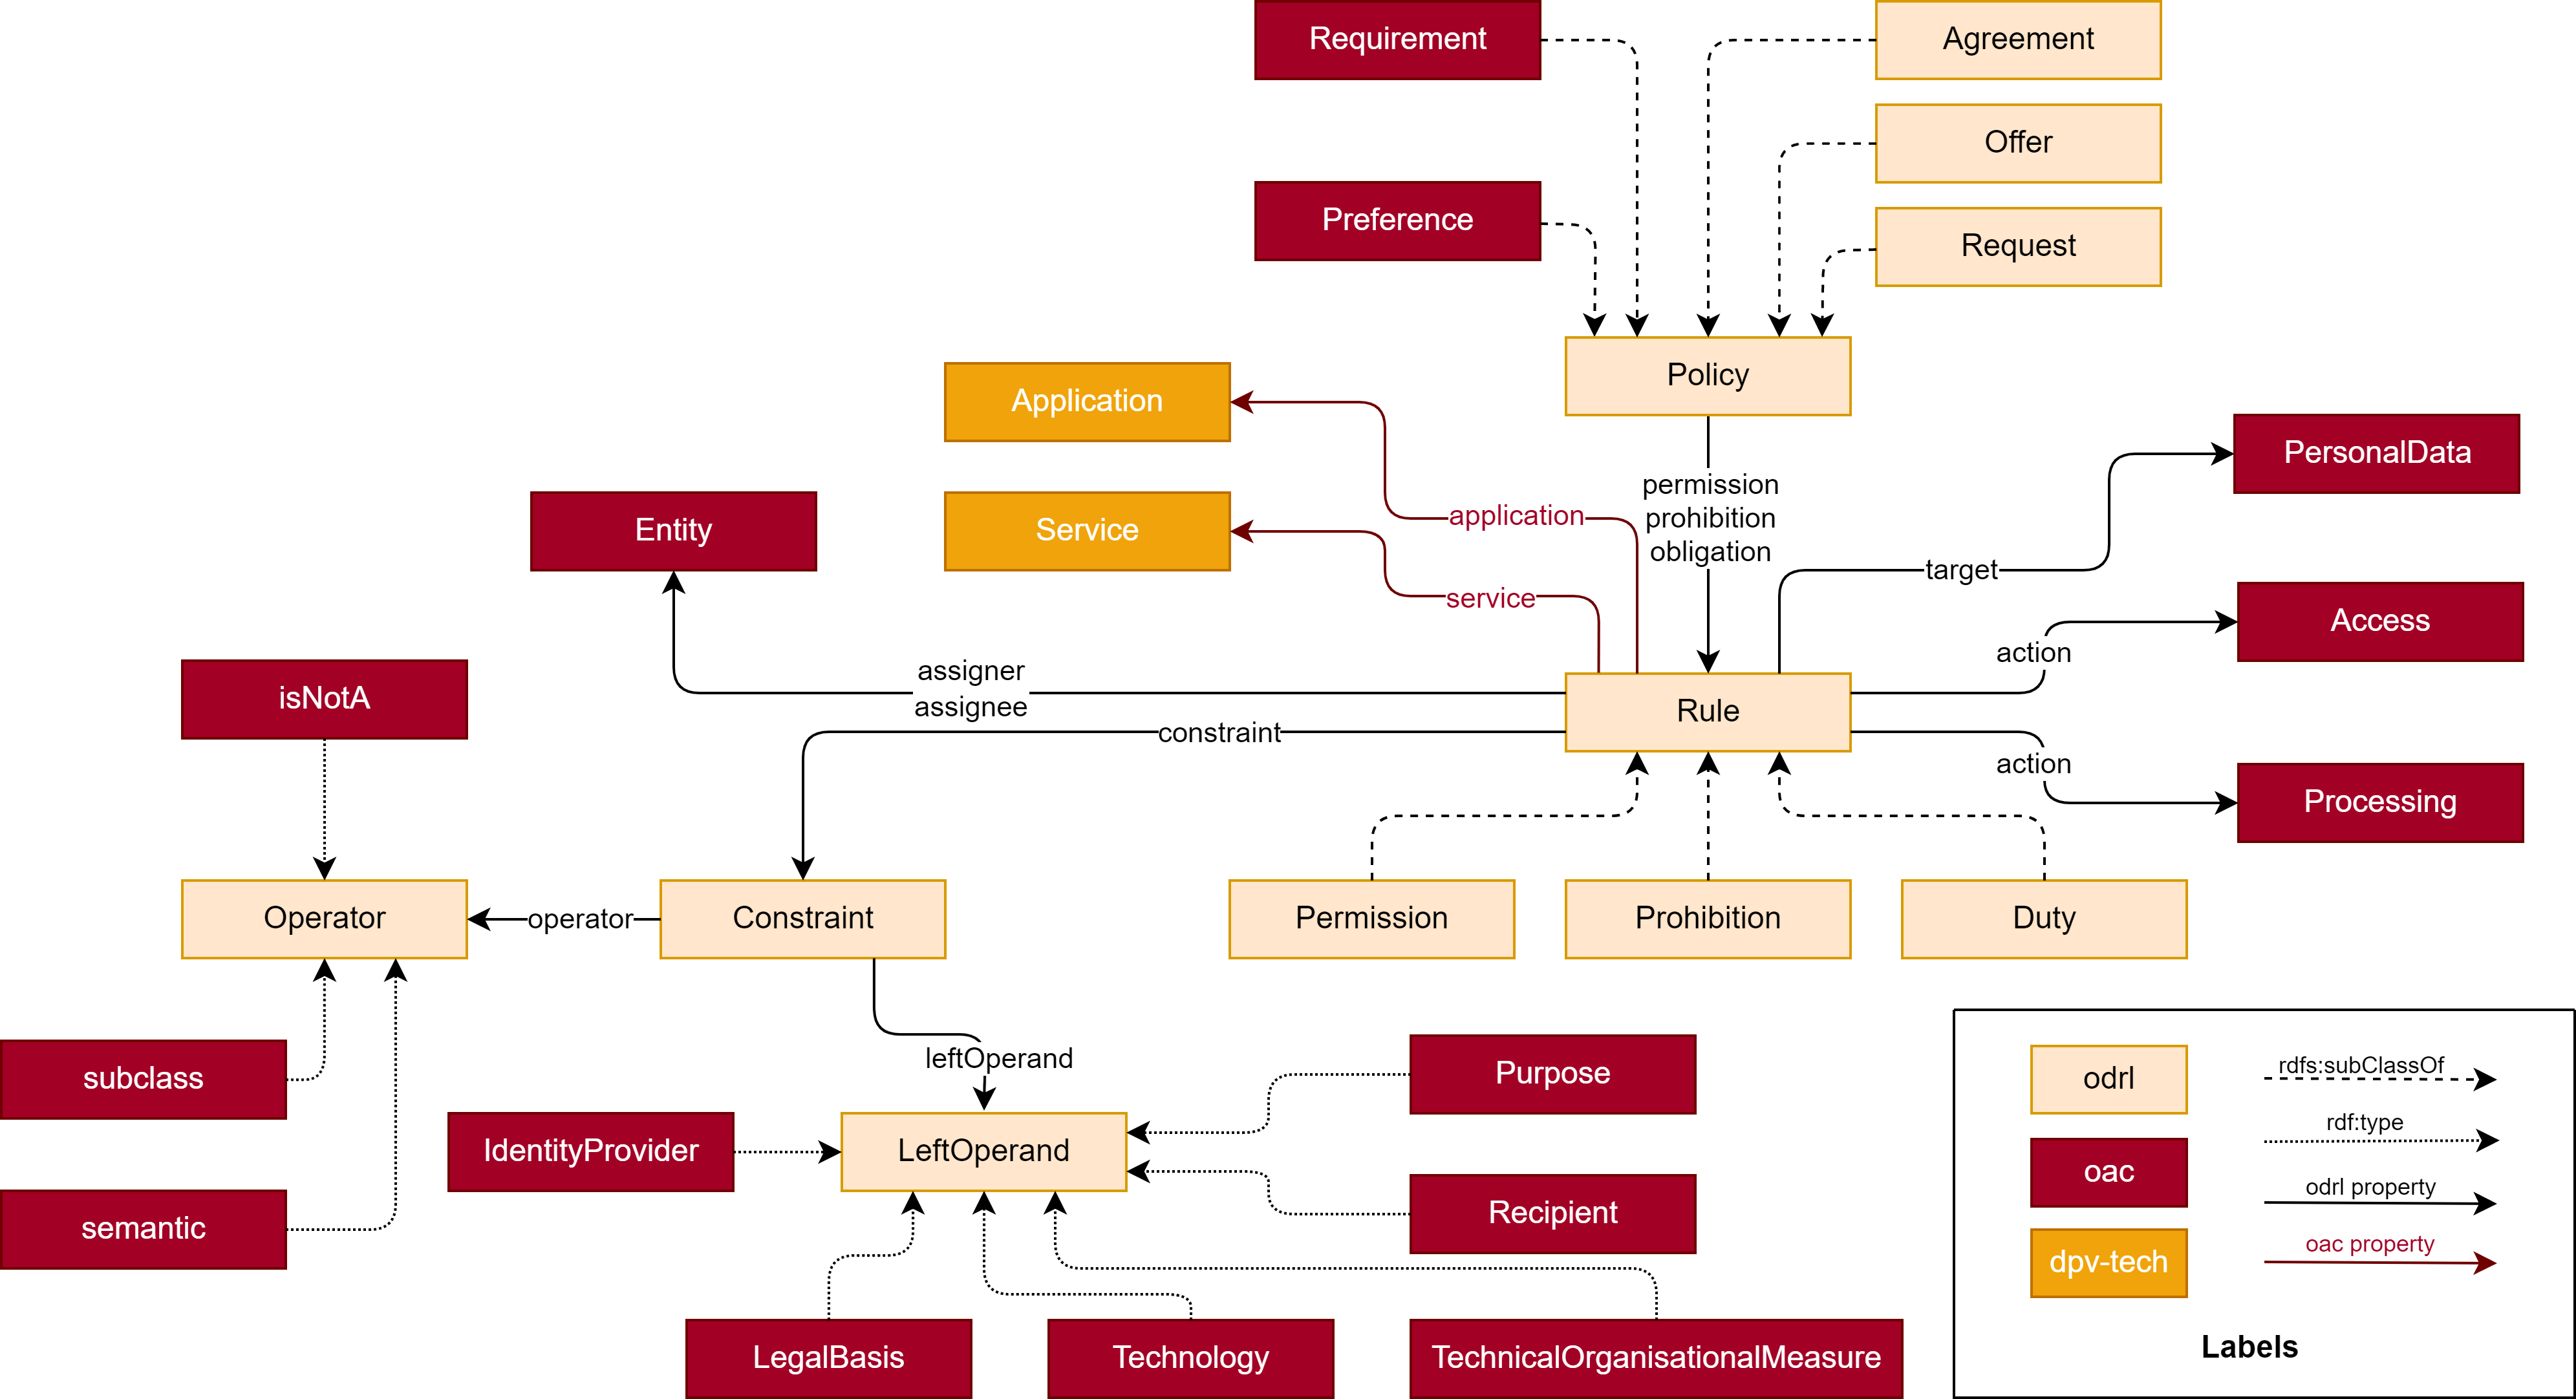
\includegraphics[width=\linewidth]{figures/chapter-4/oac_diagram.png}
    \caption{Diagrams of the concepts specified by the OAC profile.}
    \label{fig:oac_diagram}
\end{figure}

Two new types of policies, which can be combined in ODRL offers, are specified to deal with the preferences and requirements of users who wish to define rules for the processing of their personal data:

\begin{itemize}
    \item \textbf{Preference} -- Soft policy that expresses the assigner's preferences over a personal data asset which may not be satisfied and must not grant any privileges to assignees. If a preference policy set by party A does not match a request policy from party B, the request can still be accepted if party A accepts party B's request conditions.
    \item \textbf{Requirement} -- Hard policy that expresses the assigner's preferences over a personal data asset which must be satisfied and must not grant any privileges to assignees. If a requirement policy set by party A does not match a request policy from party B, the request must be denied even if party A accepts party B's request conditions.
\end{itemize}

\begin{table}[htbp]
\centering
\caption{Classes and named individuals specified in the OAC profile.}
\label{tab:profile_classes}
\resizebox{\textwidth}{!}{
\begin{tabular}{c||c|c}
Profile term & Instance of & Subclass of \\
\hline\hline
\texttt{oac:Preference} & & \texttt{odrl:Policy} \\
\hline
\texttt{oac:Requirement} & & \texttt{odrl:Policy} \\
\hline
\texttt{oac:isNotA} & \texttt{odrl:Operator} & \\
\hline
\texttt{oac:subclass} & \texttt{odrl:Operator} & \\
\hline
\texttt{oac:semantic} & \texttt{odrl:Operator} & \\
\hline
\texttt{oac:PersonalData} & \texttt{odrl:Asset} & \texttt{dpv:PersonalData} \\
\hline
\texttt{oac:Access} & \texttt{odrl:Action} & \texttt{acl:Access} \\
\hline
\texttt{oac:Processing} & \texttt{odrl:Action} & \texttt{dpv:Processing} \\
\hline
\texttt{oac:Entity} & \texttt{odrl:Party} & \texttt{dpv:Entity} \\
\hline
\texttt{oac:Purpose} & \texttt{odrl:LeftOperand} & \texttt{dpv:Purpose} \\
\hline
\texttt{oac:Recipient} & \texttt{odrl:LeftOperand} & \texttt{dpv:Recipient} \\
\hline
\texttt{oac:LegalBasis} & \texttt{odrl:LeftOperand} & \texttt{dpv:LegalBasis} \\
\hline
\texttt{oac:TechnicalOrganisationalMeasure} & \texttt{odrl:LeftOperand} & \texttt{dpv:TechnicalOrganisationalMeasure} \\
\hline
\texttt{oac:Technology} & \texttt{odrl:LeftOperand} & \texttt{dpv:Technology} \\
\hline
\texttt{oac:IdentityProvider} & \texttt{odrl:LeftOperand} & \\
\end{tabular}}
\end{table}

\begin{table}[htbp]
\centering
\caption{Properties specified in the OAC profile.}
\label{tab:profile_properties}
\begin{tabular}{c||c|c}
Profile property & Domain & Range \\
\hline\hline
\texttt{oac:service} & \texttt{odrl:Rule}, \texttt{odrl:Policy} & \texttt{dpv-tech:Service} \\
\hline
\texttt{oac:application} & \texttt{odrl:Rule}, \texttt{odrl:Policy} & \texttt{dpv-tech:Application} \\
\end{tabular}
\end{table}

Listing~\ref{list:oac_req_pref} presents an example of an OAC requirement and an OAC preference policies and Listing~\ref{list:oac_offer} an ODRL offer, based on the previously listed requirement and preference policies, as is indicated by the \texttt{dcterms:source} property.
The permission associated with the requirement policy contains the property \texttt{dpv:hasContext} associated with the term \texttt{dpv:Required} to indicate that said permission is a requirement, while the term \texttt{dpv:Optional} is used to identify the rules related with a preference policy.

\begin{listing}[htp]
\caption{OAC requirement and preference policies issued by \url{https://solidweb.me/besteves4/profile/card\#me}.}
\label{list:oac_req_pref}
\begin{minted}{turtle}
<https://solidweb.me/besteves4/policies/requirement1> a oac:Requirement ;
    odrl:uid <https://solidweb.me/besteves4/policies/requirement1> ;
    odrl:profile oac: ;
    dcterms:description "Requirement to read identifier data for identity verification purposes." ;
    dcterms:creator <https://solidweb.me/besteves4/profile/card#me> ;
    dcterms:issued "2023-10-20T18:22:15"^^xsd:dateTime ;
    odrl:permission [
        odrl:assigner <https://solidweb.me/besteves4/profile/card#me> ;
        odrl:target oac:Identifier ;
        odrl:action oac:Read ;
        odrl:constraint <#Constraint_Purpose_IdentityVerification> .

<#Constraint_Purpose_IdentityVerification> a odrl:Constraint ;
    dcterms:title "Purpose for access is to verify the identity of the assigner." ;
    odrl:leftOperand oac:Purpose ;
    odrl:operator odrl:isA ;
    odrl:rightOperand dpv:IdentityVerification .

<https://solidweb.me/besteves4/policies/preference1> a oac:Preference ;
    odrl:uid <https://solidweb.me/besteves4/policies/preference1> ;
    odrl:profile oac: ;
    dcterms:description "Preference to read age data if purpose is not commercial research." ;
    dcterms:creator <https://solidweb.me/besteves4/profile/card#me> ;
    dcterms:issued "2023-10-20T18:26:09"^^xsd:dateTime ;
    odrl:permission [
        odrl:assigner <https://solidweb.me/besteves4/profile/card#me> ;
        odrl:target oac:Age ;
        odrl:action oac:Read ;
        odrl:constraint <#Constraint_Purpose_not_CommercialResearch> .

<#Constraint_Purpose_not_CommercialResearch> a odrl:Constraint ;
    dcterms:title "Purpose for access is not commercial research." ;
    odrl:leftOperand oac:Purpose ;
    odrl:operator oac:isNotA ;
    odrl:rightOperand dpv:CommercialResearch .
\end{minted}
\end{listing}

\begin{listing}[htp]
\caption{ODRL offer issued by \url{https://solidweb.me/besteves4/profile/card\#me}.}
\label{list:oac_offer}
\begin{minted}{turtle}
<https://solidweb.me/besteves4/policies/offer1> a odrl:Offer ;
    odrl:uid <https://solidweb.me/besteves4/policies/offer1> ;
    odrl:profile oac: ;
    dcterms:description "Offer to read identifier data for identity verification and age data if purpose is not commercial research." ;
    dcterms:creator <https://solidweb.me/besteves4/profile/card#me> ;
    dcterms:source <https://solidweb.me/besteves4/policies/requirement1>, <https://solidweb.me/besteves4/policies/preference1> ;
    dcterms:issued "2023-10-20T22:15:34"^^xsd:dateTime ;
    odrl:permission [
        dpv:hasContext dpv:Required ;
        odrl:assigner <https://solidweb.me/besteves4/profile/card#me> ;
        odrl:action oac:Read ;
        odrl:target oac:Identifier ;
        odrl:constraint <#Constraint_Purpose_IdentityVerification>
    ] ;
    odrl:permission [
        dpv:hasContext dpv:Optional ;
        odrl:assigner <https://solidweb.me/besteves4/profile/card#me> ;
        odrl:action oac:Read ;
        odrl:target oac:Age ;
        odrl:constraint <#Constraint_Purpose_not_CommercialResearch>
    ] .

<#Constraint_Purpose_IdentityVerification> a odrl:Constraint ;
    dcterms:title "Purpose for access is to verify the identity of the assigner." ;
    odrl:leftOperand oac:Purpose ;
    odrl:operator odrl:isA ;
    odrl:rightOperand dpv:IdentityVerification .

<#Constraint_Purpose_not_CommercialResearch> a odrl:Constraint ;
    dcterms:title "Purpose for access is not commercial research." ;
    odrl:leftOperand oac:Purpose ;
    odrl:operator oac:isNotA ;
    odrl:rightOperand dpv:CommercialResearch .
\end{minted}
\end{listing}

Additionally, a set of three new ODRL operators, which are currently missing from the ODRL Core vocabulary Recommendation, and two new properties to specify policies applicable to certain services or applications, \texttt{oac:service} and \texttt{oac:application}, which are important stakeholders in decentralised data systems, are specified in OAC.
The newly introduced \texttt{oac:isNotA} operator is used in the \texttt{<\#Constraint\_Purpose\_not\_CommercialResearch>} constraint, in Listing~\ref{list:oac_req_pref}, to indicate that the purpose for access can not be an instance of the right operand of the constraint, e.g., \texttt{dpv:CommercialResearch}.
The \texttt{oac:subclass} operator can be used to indicate that a given left operand is a subclass of the right operand of the constraint, e.g., the purpose constraint of a rule can be a subclass of DPV's research and development purpose such as academic research, non-commercial research or commercial research, and the \texttt{oac:semantic} operator to express that a given left operand is equal to, an instance or a subclass of the right operand of the constraint, e.g., the purpose constraint of a rule can be research and development, an instance of research and development or one of its subclasses such as academic research, non-commercial research or commercial research.

Personal data is defined as an ODRL asset to define personal data-specific access policies, access modes and processing operations are defined as ODRL actions to define policies for specific access modes and/or processing operations which are not covered by ACL's access modes, e.g., \texttt{dpv:Transfer} or \texttt{dpv:Copy}, and DPV's \texttt{Entity} concept is defined as an ODRL party to define entity-specific access policies.
Additionally, when defining ODRL requests, the data requesters might use processing concepts, \texttt{dpv:Use, dpv:Collect, dpv:Share}, as the permitted/prohibited action of the rule that differ from the existing ACL's access modes, \texttt{acl:Read, acl:Write, acl:Append}.
As such, a mapping of ACL verbs to DPV processing operations is provided in OAC for such cases where offers and requests need to be matched and include both ACL access modes and DPV processing operations.
In this mapping, the \texttt{acl:Read} access mode corresponds to \texttt{dpv:Use, dpv:Collect} processing operations, and \texttt{acl:Write} resembles \texttt{dpv:Store, dpv:MakeAvailable}.
Furthermore, as previously mentioned, there are operations such as \texttt{dpv:Share} or \texttt{dpv:Transfer} that do not have a specific corresponding concept in WAC's ACL vocabulary, which require a greater introspection in the integration of legal processing concepts with access control operations.
Moreover, purposes, recipients, legal bases, technical and organisational measures, technologies and identity providers are defined as ODRL constraints to define constraint-restricted access policies.

Listing~\ref{list:oac_request} presents an example of an ODRL request that uses OAC terms and Listing~\ref{list:oac_agreement} an ODRL agreement which is the result of the matching between the offer defined in Listing~\ref{list:oac_offer} and the previously mentioned request.
In this example, Beatriz, identified by \url{https://solidweb.me/besteves4/profile/card#me}, and Arya, identified by \url{https://solidweb.me/arya/profile/card#me}, reach an agreement to allow read access operations over Beatriz's age data for the purpose of academic research in project X.
This \texttt{odrl:Agreement} is the result of the matching of \url{https://solidweb.me/besteves4/policies/offer1} and \url{https://solidweb.me/arya/requests/age_academicResearch}, as indicated by the \texttt{dcterms:references} property.
The legal basis of the agreement is consent, as is specified in the policy with the \texttt{dpv:hasLegalBasis dpv:Consent} terms, and Beatriz and Arya are registered as the data subject and data controller in question, respectively, using the \texttt{dpv:hasDataSubject} and \texttt{dpv:hasDataController} terms.
\beatriz{Policy matching and agreement generation is discussed in Chapter XX.}

\begin{listing}[ht]
\caption{ODRL request issued by \url{https://solidweb.me/arya/profile/card\#me}.}
\label{list:oac_request}
\begin{minted}{turtle}
<https://solidweb.me/arya/requests/age_academicResearch> a odrl:Request ;
    odrl:uid <https://solidweb.me/arya/requests/age_academicResearch> ;
    odrl:profile oac: ;
    dcterms:description "Request to read age data for academic research." ;
    dcterms:creator <https://solidweb.me/arya/profile/card#me> ;
    dcterms:issued "2023-10-21T13:47:56"^^xsd:dateTime ;
    odrl:permission [
        odrl:assignee <https://solidweb.me/arya/profile/card#me> ;
        odrl:action oac:Use ;
        odrl:target oac:Age ;
        odrl:constraint <#Constraint_Purpose_AcademicResearch>
    ] .

<#Constraint_Purpose_AcademicResearch> a odrl:Constraint ;
    dcterms:title "Purpose for access is to conduct academic research in project X." ;
    odrl:leftOperand oac:Purpose ;
    odrl:operator odrl:eq ;
    odrl:rightOperand ex:AcademicResearchProjectX .

ex:AcademicResearchProjectX a dpv:Purpose ;
    rdfs:subClassOf dpv:AcademicResearch ;
    rdfs:label "Conduct research in the academic project X." .
\end{minted}
\end{listing}

\begin{listing}[ht]
\caption{ODRL agreement to read age data for academic research based on consent.}
\label{list:oac_agreement}
\begin{minted}{turtle}
<https://solidweb.me/besteves4/policies/agreement1> a odrl:Agreement ;
    odrl:uid <https://solidweb.me/besteves4/policies/agreement1> ;
    odrl:profile oac: ;
    dcterms:description "Agreement to read age data for academic research based on consent." ;
    dcterms:creator <https://solidweb.me/besteves4/profile/card#me> ;
    dcterms:issued "2023-10-21T13:58:37"^^xsd:dateTime ;
    dcterms:references <https://solidweb.me/besteves4/policies/offer1>, <https://solidweb.me/arya/requests/age_academicResearch> ;
    dpv:hasDataSubject <https://solidweb.me/besteves4/profile/card#me> ;
    dpv:hasDataController <https://solidweb.me/arya/profile/card#me> ;
    dpv:hasLegalBasis dpv:Consent ;
    odrl:permission [
        odrl:assigner <https://solidweb.me/besteves4/profile/card#me> ;
        odrl:assignee <https://solidweb.me/arya/profile/card#me> ;
        odrl:action oac:Read ;
        odrl:target oac:Age ;
        odrl:constraint <#Constraint_Purpose_AcademicResearch>
    ] .
\end{minted}
\end{listing}

This Thesis focuses on \textit{Purpose, Personal Data, Processing, Recipients, Legal Bases, Technical and Organisational Measures} and \textit{Technologies} as the minimum `core concepts' for the OAC profile, and leaves out other DPV concepts such as rights or risks, which can be added at a later stage if needed.
Furthermore, similarly to WAC and ACP, OAC policies can also be defined for particular resources identified by URIs -- in such cases when an access request for a particular data type comes in, the authorisation mechanism must have information about what type of data those particular resources contain or else they will not be returned if they match the data type of the request.
Such information can be stored in a data registry, stored in a e.g. Solid Pod, where resources can be associated with the type of data they contain by using DPV's \texttt{hasPersonalData} property and DPV-PD's taxonomy of personal data categories, e.g., \texttt{<https://solidweb.me/besteves4/private/health/file1> dpv:hasPersonalData dpv-pd:HealthHistory .}

Ultimately, since these policies are stored in the personal datastore for purposes of accountability and transparency, apps and services, based on the stored preferences, requests, and agreements, can be built, e.g., using SPARQL queries, to inquire who is using what data and for what purposes.
Listing~\ref{list:sparql_agreement} presents a SPARQL query to retrieve permitted data accesses by user, data, and purpose from ODRL agreements stored in a decentralised datastore.

\begin{listing}[ht]
\caption{SPARQL query to retrieve authorised data accesses by user, data, and purpose.}
\label{list:sparql_agreement}
\begin{minted}{sparql}
SELECT DISTINCT ?User ?Data ?Purpose WHERE {
    ?a a odrl:Agreement .
    ?a odrl:permission ?perm .
    ?perm odrl:assignee ?User .
    ?perm odrl:target ?Data .
    ?perm odrl:constraint ?c .
    ?c odrl:leftOperand oac:Purpose .
    ?c odrl:operator odrl:eq .
    ?c odrl:rightOperand ?Purpose .
}
\end{minted}
\end{listing}

\subsection{Profile publication and maintenance}
\label{sec:oac_publication}

The ontology human-readable documentation and machine-readable file are available at \url{https://w3id.org/oac} using content negotiation.
The HTML documentation includes a description of the classes and properties of the ontology, that was done in collaboration with domain experts, a diagram with the graphical representation of the ontology, examples of policies defined with the OAC profile, and information related to the policy matching algorithm.
The ontology documentation also includes metadata, such as the identity of the creators and publishers of the ontology, the dates of creation and last modification, or the version number.

The source code is hosted at \url{https://w3id.org/oac/repo}, under the CC-BY-4.0 license.
The repository can also be used by OAC users to suggest new inclusions to the ontology and to report bugs through GitHub Issues.
In addition, the repository at \url{https://w3id.org/oac/policies} contains a growing collection of OAC policies that can be reused by OAC users.
% \section{Metadata language for Solid}
\label{sec:plasma}

This Section describes the development of PLASMA, a metadata language for policy-based access control in Solid, to express metadata related to the entities, registries, logs, policies and infrastructure necessary to provide transparency to Solid's data handling practices.

\subsection{PLASMA requirements specification}
\label{sec:plasma_requirements}

This Section outlines the motivation and identified requirements for the development of PLASMA, a Policy LAnguage for Solid’s Metadata-based Access control.
As previously mentioned, Solid builds upon Web's ethical principles\footnote{\url{https://www.w3.org/TR/ethical-web-principles/} (accessed on 22 October 2023)} and standards such as LDP or RDF and, in accordance with its Protocol, relies on said standards to \textit{``realise a space where individuals can maintain their autonomy, control their data and privacy, and choose applications and services to fulfil their needs''} \citep{capadisli_solid_2022}.

Although it was designed with these goals in mind, Solid currently lacks compatibility with data protection regulatory efforts \citep{pandit_making_2023}, such as the GDPR.
In particular, Solid lacks a practical mechanism to enforce GDPR's principles of transparency and accountability as there are no tools for users, applications or services to model or document information related to privacy notices, agreements, consent and rights exercising.
Furthermore, Solid is based on a ground-up redesign where machine-readable information is encouraged to be provided and reused towards improving the value of data and quality of life for users.
However, Solid's access control specifications do not contain any mechanism by which apps can provide or users can understand or express information regarding who/why/how data will be used, and to utilise these in making the process of granting and controlling access to data easier and legally compatible.
This lack of `actionable records' also strengthens the propagation of existing problems of the Web such as the use of dark patterns or manipulations to gain access to personal data of Web users.

Given that users are well versed in the usage of apps, e.g. on their smartphones, there is an expectation that Solid should also adopt an environment of trust and accountability that reduces the cognitive overload on users to understand complex information and make informed decisions, and where the environment guides responsible and accountable development.
Examples of such measures include the usage of app stores and curated or approved application verification processes.
Without these, Solid users currently have no means to identify who are the actors behind the app and authorities cannot know whom to approach when opening an investigation on faulty data practices.

Therefore, based on these considerations, the following requirements were drafted for the development of PLASMA:

\begin{enumerate}
    \item [R1.] Support specifying information about Solid infrastructure.
    \item [R2.] Record information about Pod, apps, services and data providers/developers.
    \item [R3.] Support specifying of different agreements and notices.
    \item [R4.] Record provenance information for future introspection and convenient access to data.
    \item [R5.] Provide conformance conditions to assist with legal compliance.
\end{enumerate}

As such, following the LOT methodology, these requirements are consolidated in the ORSD available in Table~\ref{tab:plasma_orsd}.
By incorporating the usage of PLASMA, Solid actors can describe their data practices in a responsible and accountable manner in a way that addresses the above-mentioned requirements.
In addition to providing the vocabulary, PLASMA also demonstrates how a \textit{decentralised ecosystem} can be developed that takes advantage of the machine-readable nature of RDF information, such as to guarantee that apps declare a set of metadata before being allowed access to data, and ensures that apps, services, agents, Pods and users act in conformance and provide an environment of trust and accountability.

\begin{table}[htbp]
\centering
\caption{Ontology Requirement Specification Document of PLASMA.}
\label{tab:plasma_orsd}
\scriptsize
\begin{tabular}{| l | l | l | l  | l | l | l |l| }
\hline
\multicolumn{8}{|c|}{\cellcolor[HTML]{A0A0A0}\textbf{Policy LAnguage for Solid’s Metadata-based Access control}} \\ \hline
\multicolumn{8}{|c|}{\cellcolor[HTML]{EFEFEF}\textbf{1. Purpose}} \\ \hline
\multicolumn{8}{| p{12.0cm} |}{The purpose of PLASMA is to provide consistent taxonomies to describe the entities, infrastructure, policies, notices, registries and logs necessary to understand and establish responsibilities and accountability within the Solid ecosystem.} \\ \hline
\multicolumn{8}{|c|}{\cellcolor[HTML]{EFEFEF}\textbf{2. Scope}} \\ \hline
\multicolumn{8}{| p{12.0cm} |}{The scope of this ontology is limited to the definition of a metadata language to provide transparency Solid's data handling practices. PLASMA promotes the usage of OAC to determine access control to Solid Pod's resources, provides conformance conditions and workflow scenarios where PLASMA terms should be used.} \\ \hline
\multicolumn{8}{|c|}{\cellcolor[HTML]{EFEFEF}\textbf{3. Implementation Language}} \\ \hline
\multicolumn{8}{| p{12.0cm} |}{RDF, RDFS} \\ \hline
\multicolumn{8}{|c|}{\cellcolor[HTML]{EFEFEF}\textbf{4. Intended End-Users}} \\ \hline
\multicolumn{8}{| p{12.0cm} |}{Developers of Solid servers, applications, services or agents.} \\ \hline
\multicolumn{8}{|c|}{\cellcolor[HTML]{EFEFEF}\textbf{5. Intended Uses}} \\ \hline
\multicolumn{8}{| p{12.0cm} |}{
Use 1. Describing entities, infrastructure and processes involved in the Solid ecosystem. \newline 
Use 2. Expressing information regarding legal roles and other compliance requirements in a jurisdiction-agnostic manner (while satisfying requirements from GDPR). \newline
Use 3. Defining patterns for the expression of users and apps policies, data use logs, and registries to provide easy access to data in Pods. 
 } \\ \hline
\multicolumn{8}{|c|}{\cellcolor[HTML]{EFEFEF}\textbf{6. Ontology Requirements}} \\ \hline
\multicolumn{8}{|c|}{\cellcolor[HTML]{EFEFEF}\textbf{a. Non-Functional Requirements}}    \\ \hline
\multicolumn{8}{| p{12.0cm} |}{
NFR 1. The ontology is published online with HTML documentation, following W3C's specification format. } \\ \hline
\multicolumn{8}{|c|}{\cellcolor[HTML]{EFEFEF}\textbf{b. Functional  Requirements: Groups of Competency Questions}}  \\ \hline
\multicolumn{8}{|p{12.0cm}|}{
CQ1. Which Pod management data is stored in the Pod? \newline
CQ2. Which metadata should be recorded when data is added/updated/removed to/from the Pod? \newline
CQ3. What data, including policies, are available in the Pod? \newline 
CQ4. What policy describes the data access requirements of a certain app or service? \newline 
CQ5. Who are the parties providing Pod infrastructure? \newline 
CQ6. How and where is the data being physically stored? \newline 
CQ7. What registries are available in the Pod for convenient access to data? \newline
CQ8. What identification information needs to be provided by Solid-involved parties? \newline 
CQ9. Which information about personal data processing is necessary to have legally aligned decentralised datastores?
}\\ \hline
\end{tabular}
\vspace{-0.1in}
\end{table}

\subsection{PLASMA taxonomies}
\label{sec:plasma_taxonomies}

PLASMA relies on OAC for the expression of policies related to access to personal data stored in Solid Pods, on the W3C Recommendation DCAT (Data CATalog vocabulary) \citep{albertoni_data_2020} for the expression of data registries and related data sets, on DCMI Metadata Terms \citep{dcmi_usage_board_dcmi_2020} for the specification of authorship, temporal and other types of provenance metadata, and on the W3C Recommendation Activity Streams 2.0 \citep{snell_activity_2017} for logging relevant events associated with Solid processes.
These design choices are aligned with the best practices described in the Data on the Web Best Practices document \citep{loscio_data_2017}.
Moreover, while there are legal vocabularies focusing on personal data protection, such as DPV and DPV-GDPR \citep{panetto_creating_2019}, these are not directly applicable to the Solid ecosystem as the terminology used is not the same, e.g., in Solid, the entity the data belongs/refers to is called \textit{`owner'}, whereas the equivalent term under the GDPR is \textit{`data subject'}.
As such, PLASMA provides additional taxonomies to describe the actors, artifacts, and processes involved in the usage of Solid Pods, apps and services, which are not modelled in the previously mentioned vocabularies.
Later on, these can be used to align with their equivalent legal terms (from the GDPR).

Thus, PLASMA supports the implementation of a new \textit{`policy layer'} which aids users, apps and Pod infrastructure providers to express relevant information about their activities in the form of machine-readable policies, logs and registers of data.
Such sources of information can then be used to enable the development of dashboards for user policy management, machine-readable notifications regarding changes in policies or data, usage of agents to automate tasks or other interfaces to understand what is being done with the Pod's data.

Figure~\ref{fig:solid_plasma} illustrates the core entities and infrastructure of the Solid ecosystem as specified in PLASMA.
Thus, the base PLASMA concepts are defined below as:

\begin{itemize}
    \item \textbf{App} -- An application that stores, collects, uses, shares, erases, or performs other actions on Data with the aim of providing specific purposes, services, or functionalities. An application can use several Services and requires human intervention.
    \item \textbf{Service} -- A functionality that may or may not utilise or interact with Data within a Pod. Services represent an abstraction of functionality that does not necessarily have to be packaged as an App.
\end{itemize}

\begin{landscape}
\begin{figure}[htbp]
    \centering
    \includegraphics[width=\linewidth]{figures/chapter-4/solid-infrastructure-actors.png}
    \caption{Core entities and infrastructure of the Solid ecosystem specified in PLASMA.}
    \label{fig:solid_plasma}
\end{figure}
\end{landscape}

\begin{itemize}
    \item \textbf{Pod} -- A Personal Data Store that conforms to the Solid Specification.
    \item \textbf{Agent} -- A virtual entity associated with carrying out actions within or related to a Pod or its Data.
    \item \textbf{Policy} -- A set of guidelines or decisions or recommendations governing the use of Pod or its Data.
    \item \textbf{Data} -- Data stored on a Pod or associated with a User, App, Service, or Data Subject of a Pod.
    \item \textbf{Entity} -- A legally recognised entity. Legally recognised means the entity has some recognition as being able to enter into agreements, has an address for accountability, and is responsible for obligations and/or rights. Entities are associated with Apps, Services, or Pods.
    \item \textbf{Solid Platform} -- The specific implementation of Solid that is installed or used within a Pod.
    \item \textbf{Solid Specification} -- The specification that the Pod conforms to in terms of defining the terms, behaviour, and implementation details regarding Pods and their association with Services and Apps.
\end{itemize}

These terms result from a thorough review of the existing Solid technical documents, in particular of the specifications related to the authorisation protocol, described in Section~\ref{sec:sota_solid_access_control}.
While they are mentioned in these specifications, only a slim fraction of them are actually defined in machine-readable form, e.g., ACP provides a \texttt{Policy} term and SAI provides a definition for \texttt{Application}.
Since no concepts were found in the existing Solid vocabularies to define what Pods, services, entities or data, PLASMA provides these terms and extends them with additional taxonomies to cover a wide set of use cases.

Therefore, in the remainder of this Section, an overview of the taxonomies of entities, policies and notices, services, and data defined in the PLASMA vocabulary is provided.

\paragraph{Entities}
Beyond the agent, client application and identity issuer predicates defined in WAC and/or ACP, there are no other terms to describe the entities involved in the Solid ecosystem.
As such, terms to describe the providers and/or developers of Solid apps, services, and other Solid-related processes and infrastructure are provided in PLASMA, as well as terms to describe different types of users and agents.
Distinct concepts for providers and developers are specified to distinguish between entities providing the infrastructure, Pods, identity, apps or services, and entities developing them (in case the distinction needs to be made), e.g., when directly using a service from the developer's website, the developer is the same as the provider, however, if a service is being used through a service store or a common marketplace, then the developer is different from the provider and both concepts should be clarified in Solid for a proper allocation of responsibilities.

Furthermore, regarding Solid-related users, an \texttt{AdminUser} is defined as a \textit{``User of a Pod that has the administrative capability to make decisions about Data on a Pod''}, i.e., can define who has access to all or parts of Data stored on a Pod, and a \texttt{PodAdmin} as a \textit{``User of a Pod that has the administrative capability to make decisions about the Pod (separate from Data in a Pod), such as deleting the Pod, changing identity or other resource providers''}, to effectively distinguish between users who fully control data and users who fully control Pods. This feature is currently missing from the Solid protocol.
With regards to the specification of agents, PLASMA departs from Solid's current definition of agent as presently, according to Solid's specifications, they can either be real or virtual agents, e.g., parents on behalf of children or software agents.
In PLASMA, agents are \textit{virtual agents}, that can act on behalf of users, apps or services, to distinguish them from entities, which can be held legally responsible.

Figure~\ref{fig:plasma_entities} illustrates the providers, developers, users and agents defined in PLASMA.

\begin{figure}[htbp]
    \centering
    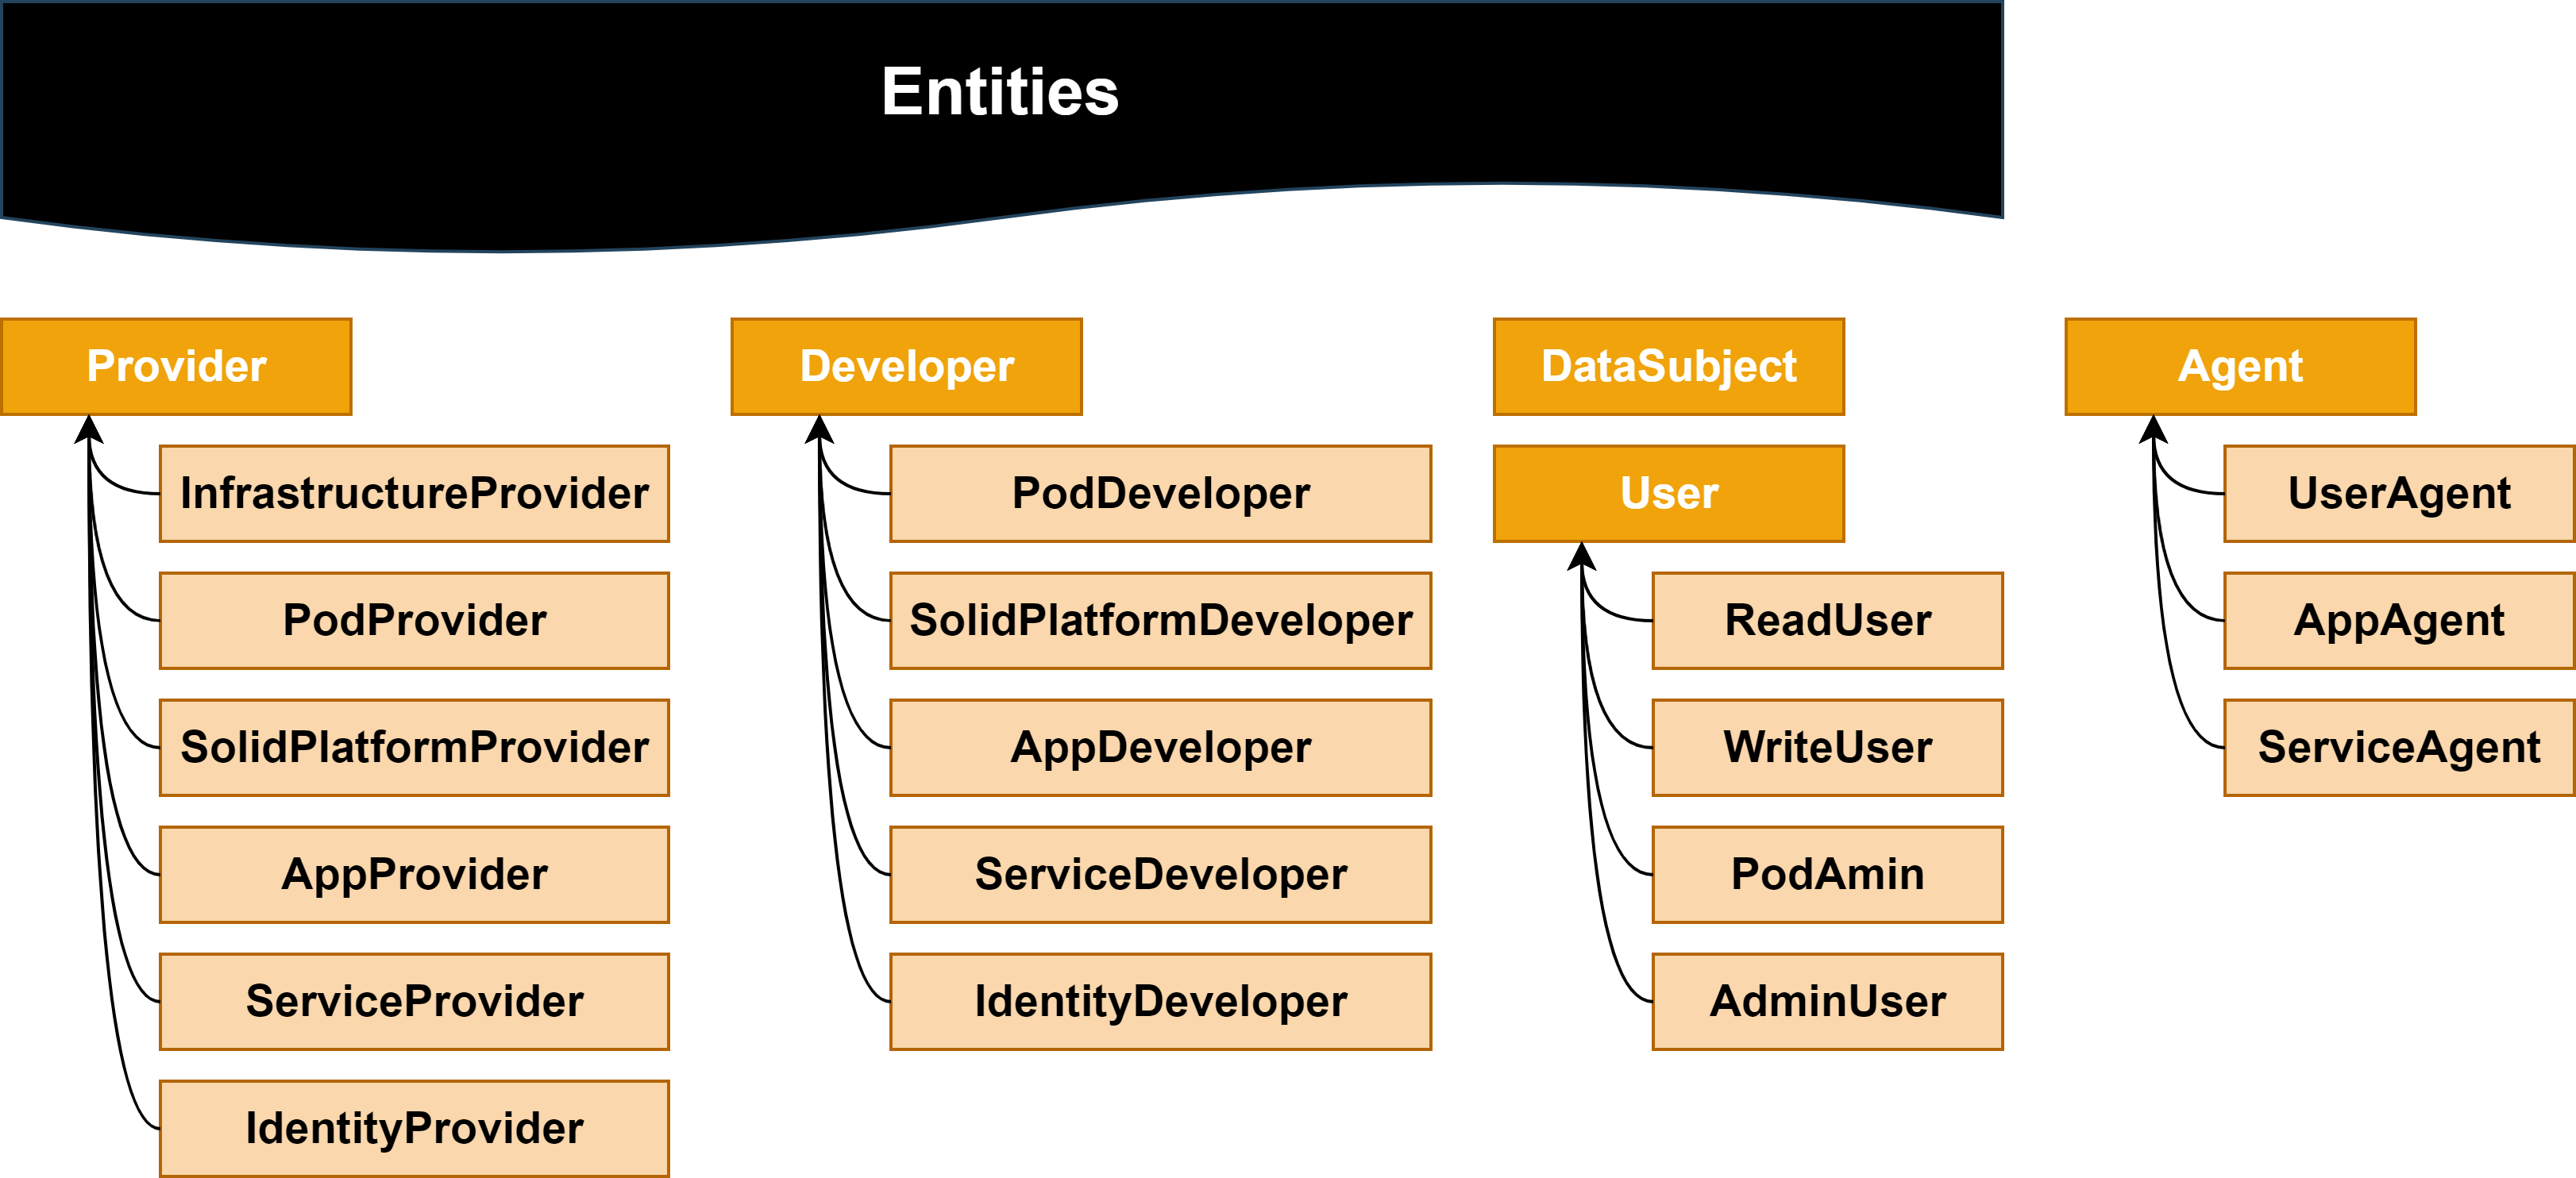
\includegraphics[width=\linewidth]{figures/chapter-4/entities.png}
    \caption{Entities and agents specified in PLASMA.}
    \label{fig:plasma_entities}
\end{figure}

\paragraph{Policies and notices}
In PLASMA, a policy is a document that specifies user, application, and service requirements for data handling practices that apply to data stored or shared through Solid Pods.
Thus, this definition is not limited to access to data stored on a Pod, it also relates to used or transferred data, i.e., to avoid cases such as data collected for purpose X being used for purpose Y.
Such a definition aids with the alignment with legal requirements, e.g., it requires that all purposes must be stated at the time of data collection and that requesters need new consent from the data subject if the purpose for access changes.
PLASMA provides definitions for user policies, in particular for user offers, requirements and preferences, aligned with the \texttt{odrl:Offer}, \texttt{oac:Requirement} and \texttt{oac:Preference} concepts described in Section~\ref{sec:oac}.
Regarding data requests, i.e., conditions for apps and services to have access to or use Pod data, PLASMA envisions their integration into the ecosystem by declaring them in a manifest such as the one being conceived in the W3C Web Application Manifest specification -- an application manifest is a \textit{``JSON document that contains startup parameters and application defaults for when a web application is launched''} \citep{manifest_2023}.
However, the current specification is not enough to achieve legal compliance as it does not include information on entities developing the app, their identity and contact details or their privacy policies.
Thus, PLASMA includes app manifest and service manifest concepts.
In addition to user policies and data requests, PLASMA also provides different types of data agreements, a concept that is completely missing from the Solid specifications as they only provide concepts to refer to apps and users' access authorisations.
As such, an agreement can either be based on the user's consent, or governed by a contract between the user and the entity having responsibility for the app, service or Pod.

Additionally, current Solid specifications also lack the definition of notices.
Notices are documents that provide context information about entities, operations, or data involved in specific processes, e.g., notices may specify the providers, developers, and/or data handling practices of applications and services. 
In this regard, PLASMA provides terms for declaring \textit{ex-ante} and \textit{ex-post} notices, as well as privacy notices for Pods, users, applications and services.

Figure~\ref{fig:plasma_policies} illustrates the policies and notices concepts specified in PLASMA.

\begin{figure}[htb]
    \centering
    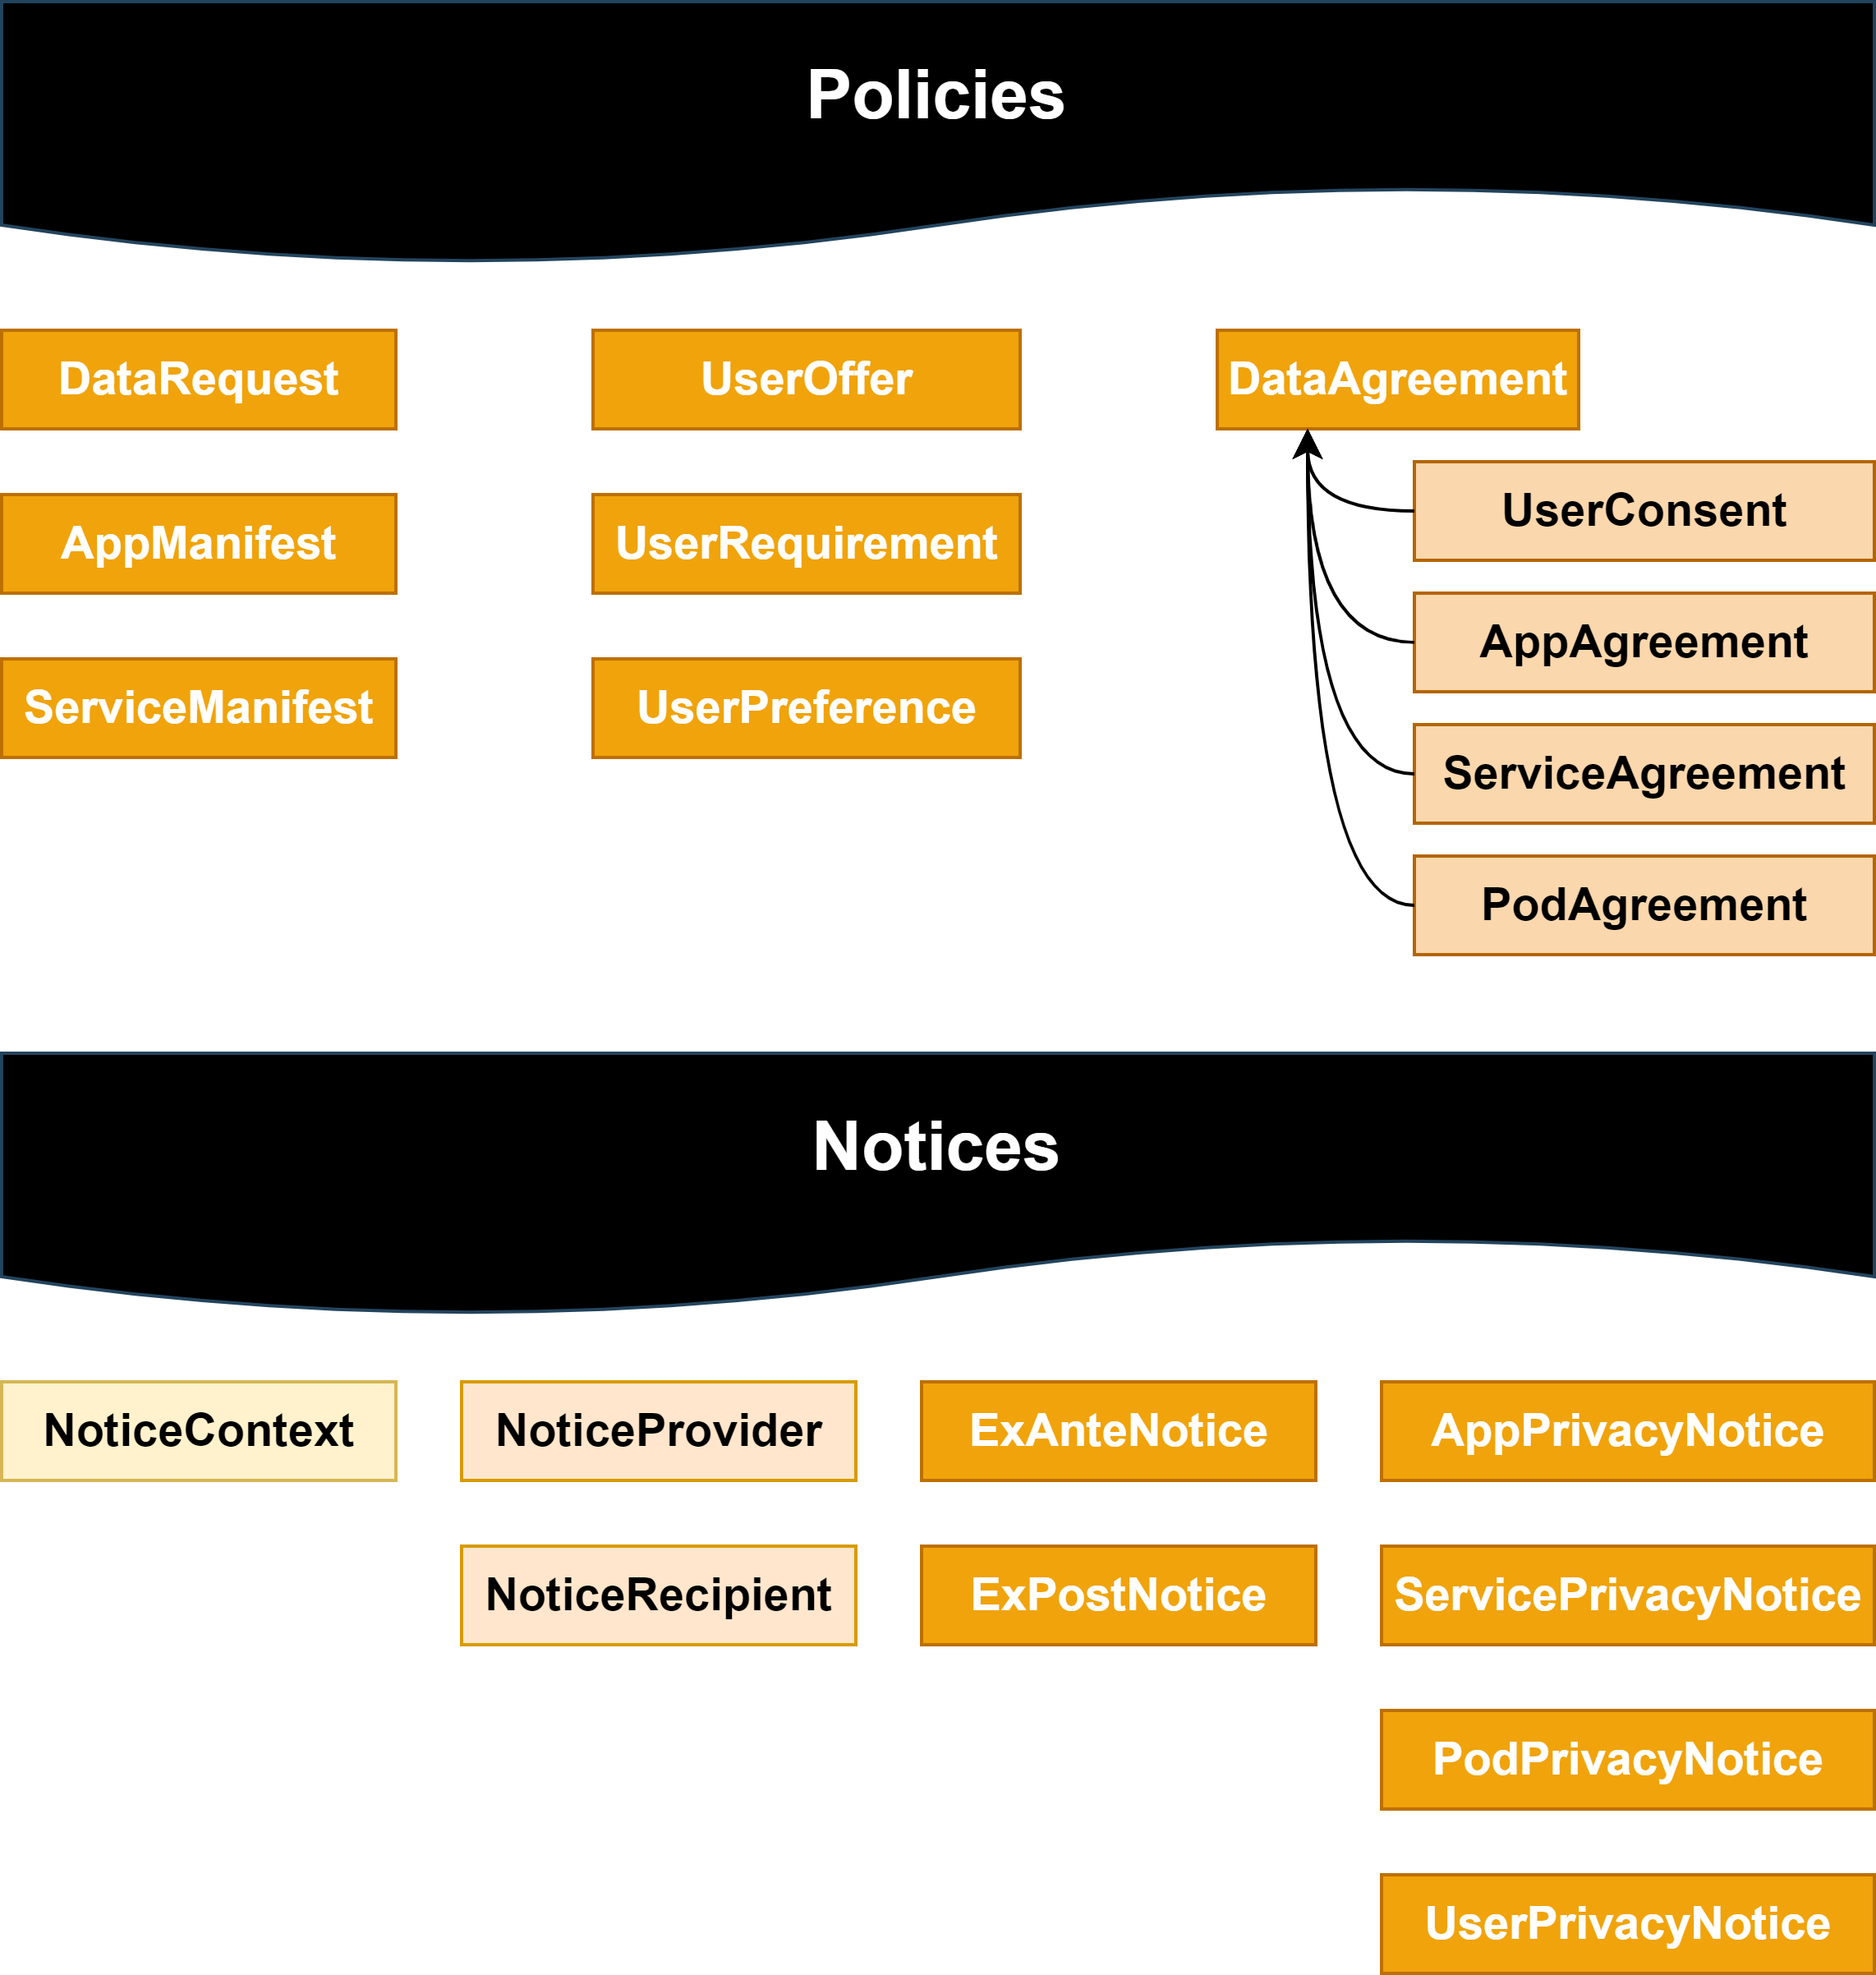
\includegraphics[width=0.8\linewidth]{figures/chapter-4/policies_notices.png}
    \caption{Policy types and notices specified in PLASMA.}
    \label{fig:plasma_policies}
\end{figure}

\paragraph{Services}
PLASMA differentiates between an app and a service -- services convey functionalities that do not need to be packaged as an app.
Moreover, an app requires human intervention to perform some action on data for a specific purpose, while a service may not require human intervention to use or interact with data within a Pod.
Since services are a new concept being introduced by PLASMA in the Solid ecosystem, a taxonomy of twelveu Solid-related services, which can be further expanded, is supplied and illustrated in Figure~\ref{fig:plasma_services}.

\begin{figure}[htb]
    \centering
    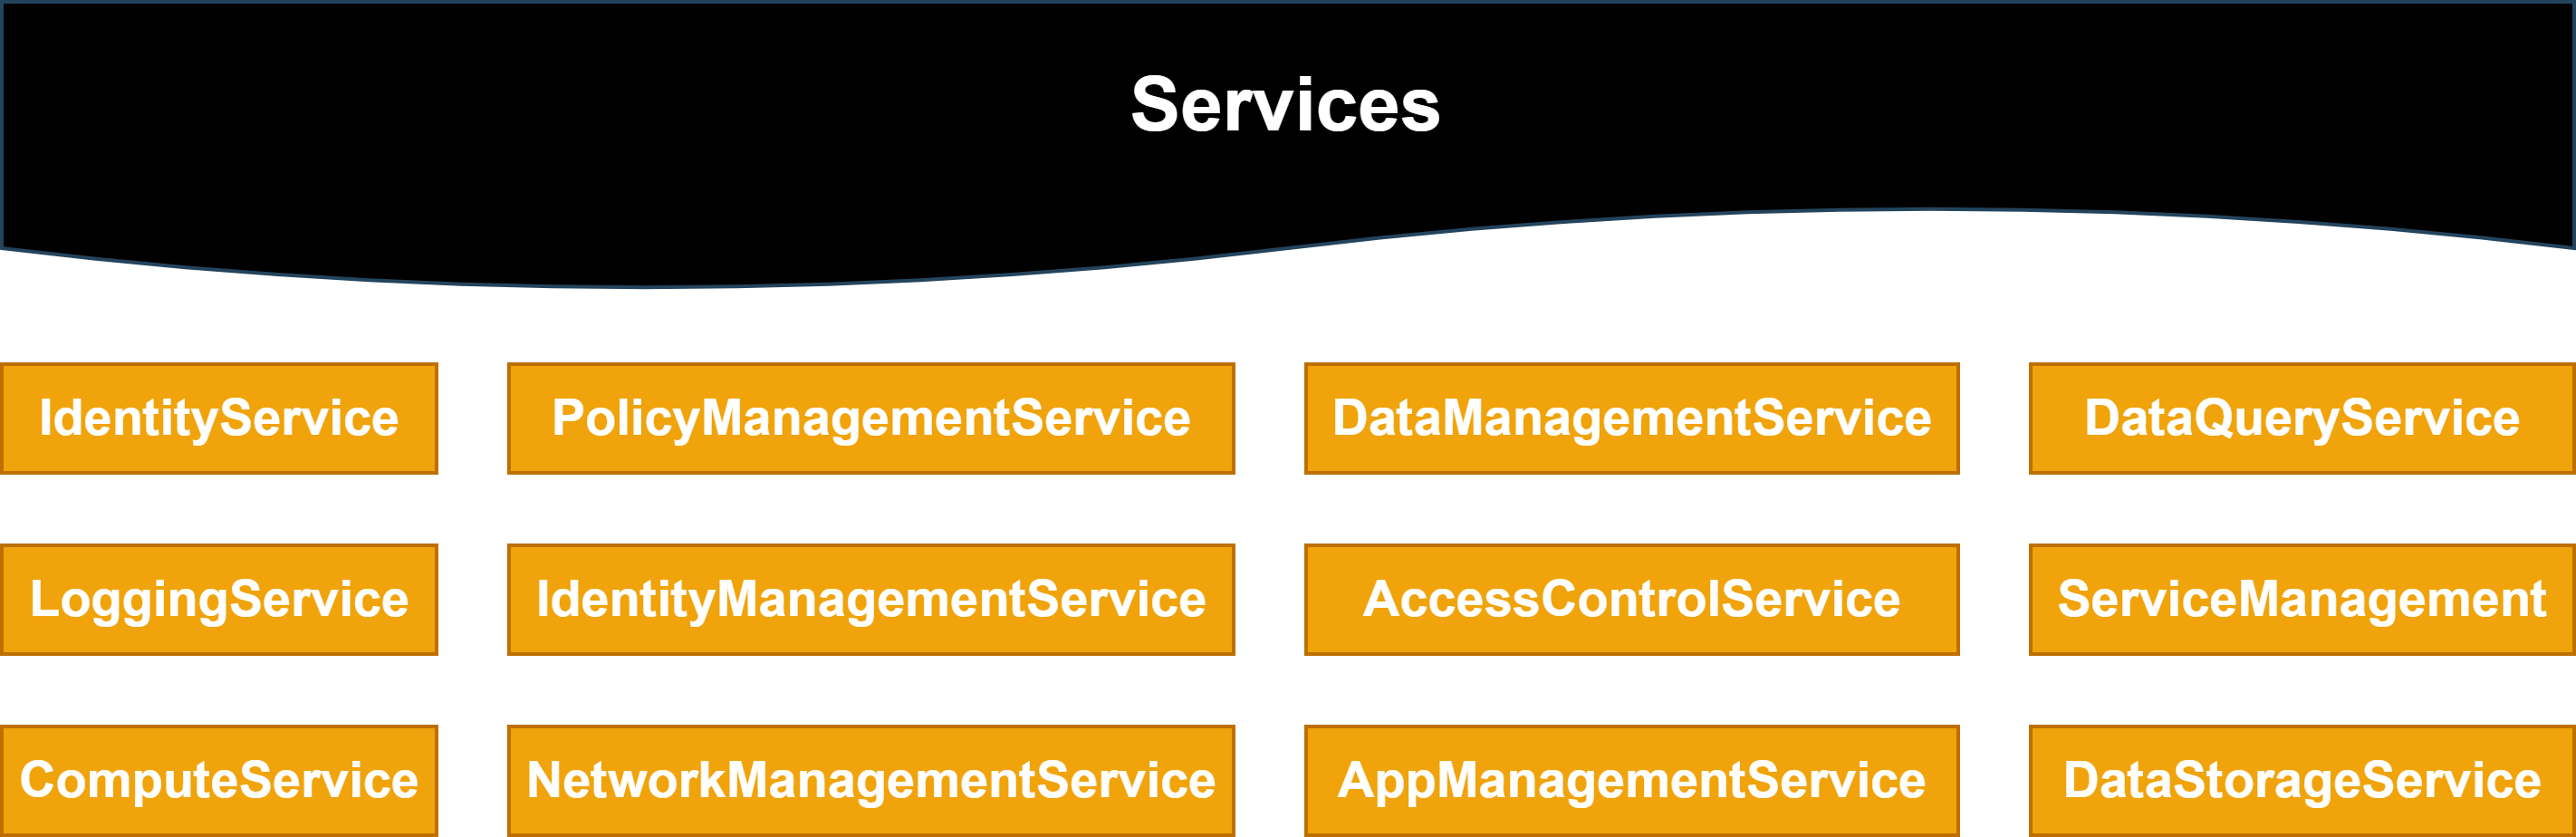
\includegraphics[width=\linewidth]{figures/chapter-4/services.png}
    \caption{Services specified in PLASMA.}
    \label{fig:plasma_services}
\end{figure}

\paragraph{Pod-related data}
To fulfil Solid's vision of providing individuals with a decentralised data storage service for their data and the choice of which applications or services to use for a specific task, metadata regarding Pod management, entities, apps, services, logs and registries should be provided.
Additionally, supervisory authorities can use such logging and provenance metadata, from the Pods of users, for auditing activities, e.g., an EU data protection authority can use these records to investigate a personal data breach.
To this end, PLASMA includes a collection of Solid-related log terms to record provenance information related to processes such as adding or updating resources in a Pod, i.e., a \texttt{DataLog}, registering a policy negotiation procedure reliant on user consent, i.e., a \texttt{PolicyLog}, or recording a successful user login operation, i.e., a \texttt{IdentityLog}.
Furthermore, the maintenance of registries as indexed records for providing collective and convenient access to data within a Pod is of the utmost importance for users, apps and services to have knowledge of the availability of data categories, supported schemas for data, apps, services, relevant policies and users that have/had access to data stored within a Pod.

Figure~\ref{fig:plasma_data} illustrates the Pod-related data concepts defined in PLASMA, including logs and registries.

\begin{figure}[htbp]
    \centering
    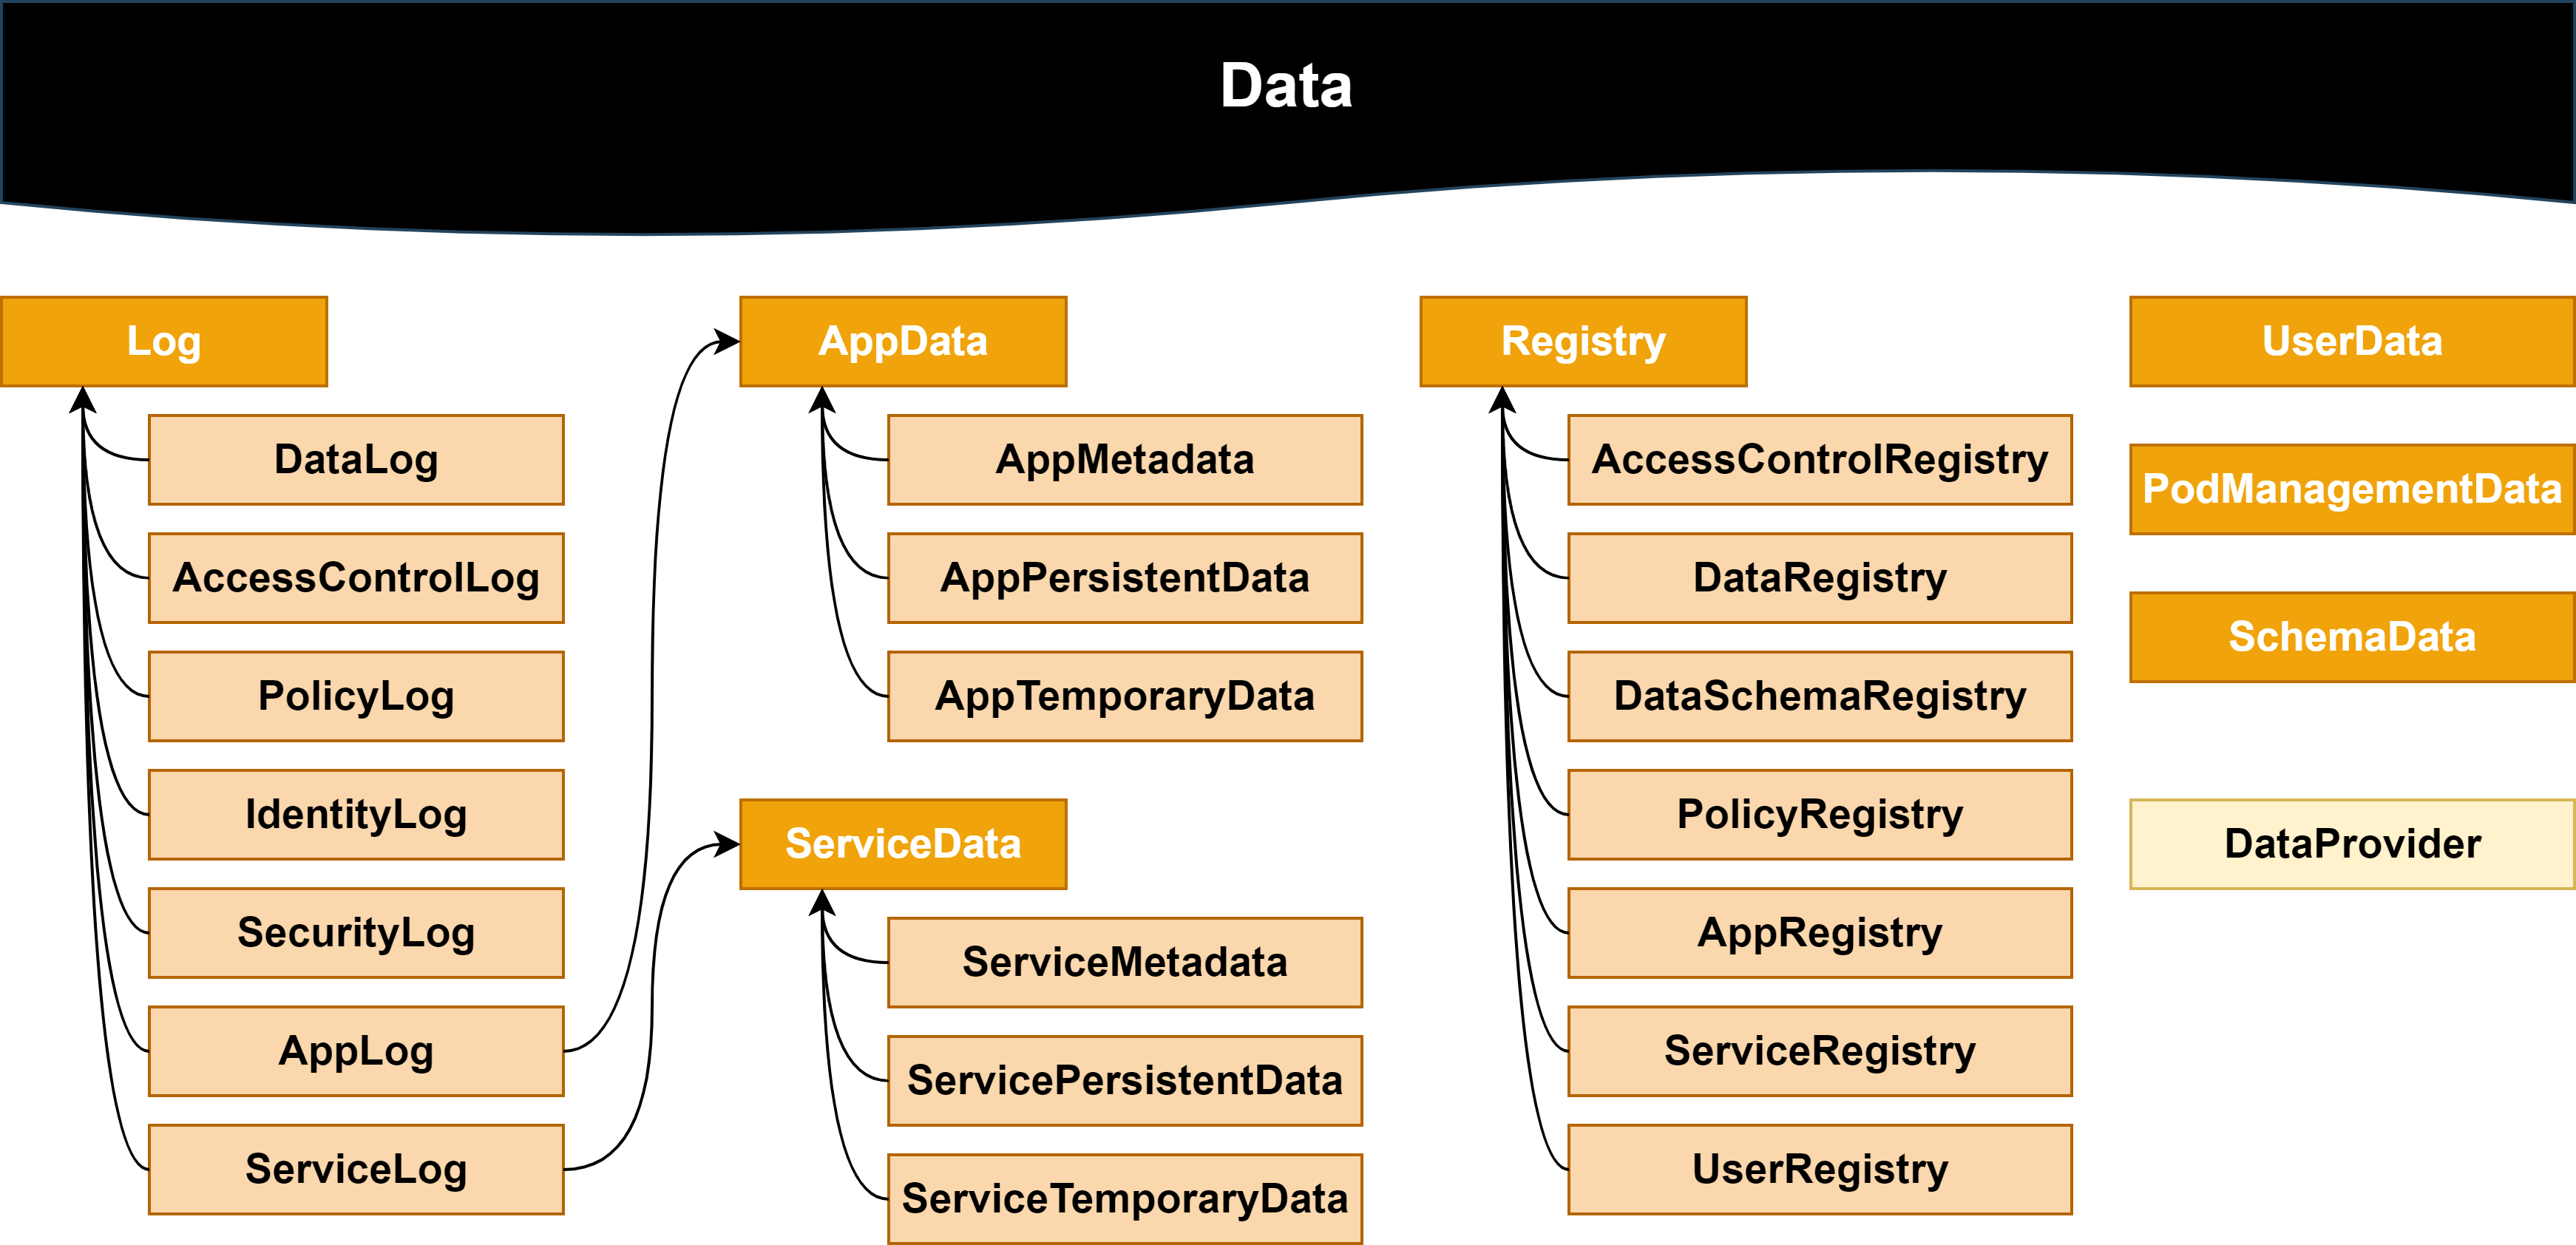
\includegraphics[width=\linewidth]{figures/chapter-4/data.png}
    \caption{Data concepts, including logs and registries, specified in PLASMA.}
    \label{fig:plasma_data}
\end{figure}

\subsection{Conformance with PLASMA}
\label{sec:plasma_conformance}

In this Section, the conditions for Pods, apps, services, users and agents to be conformant with PLASMA are described, including information regarding what is mandatory (indicated below by the use of the word \textit{`must'}) or optional (indicated below by the use of the word \textit{`may'}) to be provided, and how conformity should be evaluated and assured by implementers of the PLASMA specification.

The W3C Recommendation on Data on the Web Best Practices, which is aimed at the \textit{``publication and usage of data on the Web designed to help support a self-sustaining ecosystem''} \citep{loscio_data_2017}, was followed for the publication of metadata related to provenance, licensing and versioning of data.
The vocabulary specifications for particular tasks, recommended by this best practices document, are mentioned in the following paragraphs.

\paragraph{Pod conformance}
For a Pod to be conformant with the PLASMA specification, the following conditions should be satisfied:

\begin{itemize}
    \item A Pod \textit{must} provide or declare \texttt{PodManagementData} which includes metadata about the Pod and of its providers and/or developers, as well as the specific \texttt{SolidPlatform} and \texttt{SolidSpecification} implemented in the Pod and any \texttt{PodAgreement} in place. Listing~\ref{list:plasma_PodManagementData} provides an example of the declaration of such metadata.
    \item A Pod \textit{must} implement or provide equivalent functionality to support the different registries and logs specified in PLASMA. Listing~\ref{list:plasma_dataschemaregistry} provides an example of a data schema registry that records data schemas, formats or shapes recognised or supported by Pods, apps or services, as indicated by the \texttt{plasma:supportedBy} property.
    \item A Pod \textit{may} have multiple users with varying degrees of control. A record of the different users and their level of access \textit{must} be kept in the \texttt{UserRegistry}.
    \item A Pod \textit{may} have discovery methods for users to make their data publicly available.
\end{itemize}

In addition to the ODRL and DCMI Metadata Terms vocabularies, the DPV's \texttt{hasName}, \texttt{hasContact} and \texttt{hasAddress} properties should be used to identify and provide contact details of the Pod, Solid platform and infrastructure providers and developers. \textit{Schema.org} and the Provenance, Authoring and Versioning (PAV) vocabularies, along with the previously mentioned DCMI, are used to describe the authors, sources, version and code repository URIs of the platform and specification installed within the Pod. \textit{Schema.org} provides an upper vocabulary of terms to describe \textit{``entities, relationships between entities and actions''} related to structured data on the Web \citep{guha_schemaorg_2015} and PAV is a \textit{``lightweight ontology for tracking Provenance, Authoring and Versioning''} that \textit{``specializes the W3C provenance ontology PROV-O in order to describe authorship, curation and digital creation of online resources''} \citep{ciccarese_pav_2013}.

\begin{listing}[htp]
\caption{Metadata of Beatriz's Pod.}
\label{list:plasma_PodManagementData}
\begin{minted}{turtle}
<https://solidweb.me/besteves4/PodMetadata> a plasma:PodManagementData ;
    dcterms:description "Metadata of Beatriz's Pod" ;
    odrl:hasPolicy <https://solidweb.me/besteves4/agreements/Pod> ;
    plasma:hasProvider <https://solidweb.me/besteves4/entities/PodProvider> ;
    plasma:hasProvider <https://solidweb.me/besteves4/entities/PlatformProvider> ;
    plasma:hasProvider <https://solidweb.me/besteves4/entities/InfrastructureProvider> ;
    plasma:implementedSolidPlatform <https://solidweb.me/besteves4/Platform> ;
    plasma:implementedSolidSpecification <https://solidweb.me/besteves4/SolidSpec> .

<https://solidweb.me/besteves4/agreements/Pod> a plasma:PodAgreement .

<https://solidweb.me/besteves4/entities/PodProvider> a plasma:PodProvider ;
    dpv:hasName "Entity A" ; dpv:hasContact "mailto:entity_a@mail.com" ;
    dpv:hasAddress "Address of Entity A" .

<https://solidweb.me/besteves4/entities/PlatformProvider> a plasma:SolidPlatformProvider .

<https://solidweb.me/besteves4/entities/InfrastructureProvider> a plasma:InfrastructureProvider .

<https://solidweb.me/besteves4/Platform> a plasma:SolidPlatform ;
    plasma:hasProvider <https://solidweb.me/besteves4/entities/PlatformProvider> ;
    dcterms:source <https://communitysolidserver.github.io> ;
    dpv:hasPolicy <https://www.serverproject.de/files/solidweb_me_terms.txt> ;
    schema:codeRepository <https://github.com/CommunitySolidServer/CommunitySolidServer> ;
    pav:version "6.1.0" ;
    dcterms:license <https://dalicc.net/licenselibrary/MIT> .

<https://solidweb.me/besteves4/SolidSpec> a plasma:SolidSpecification ;
    dcterms:conformsTo <https://solidproject.org/TR/2022/protocol-20221231> ;
    dcterms:creator "Sarven Capadisli", "Tim Berners-Lee", "Ruben Verborgh", "Kjetil Kjernsmo" ;
    dcterms:license <https://dalicc.net/licenselibrary/MIT> ;
    pav:version "0.10.0" ; dcterms:created "2022-12-31"^^xsd:date ;
    schema:codeRepository <https://github.com/solid/specification> .
\end{minted}
\end{listing}

\begin{listing}[htp]
\caption{Data schema registry of Beatriz's Pod.}
\label{list:plasma_dataschemaregistry}
\begin{minted}{turtle}
<https://solidweb.me/besteves4/SchemaRegistry> a plasma:DataSchemaRegistry ;
    dcterms:description "Registry listing recognised or supported schemas" ;
    dcterms:created "2023-09-10T11:51:17"^^xsd:dateTime ;
    dcterms:modified "2023-10-07T12:39:50"^^xsd:dateTime ;
    dcterms:publisher <https://solidweb.me/besteves4/entities/DataMgtServiceProvider> ;
    plasma:hasSchema <https://solidweb.me/besteves4/schemas/EHR-schema>,
        <https://solidweb.me/besteves4/schemas/img-format>,
        <https://solidweb.me/besteves4/schemas/entity-shape> .

<https://solidweb.me/besteves4/entities/DataMgtServiceProvider> a plasma:ServiceProvider ;
    plasma:serviceType plasma:DataManagementService ;
    dpv:hasName "Entity A" ;
    dpv:hasAddress "Address of Entity A" ;
    dpv:hasContact "mailto:entity_a@mail.com" .

<https://solidweb.me/besteves4/schemas/EHR-schema> a plasma:SchemaData ;
    dcterms:conformsTo <http://www.w3.org/TR/turtle/> ;
    plasma:supportedBy <https://example.com/health-service> .

<https://example.com/health-service> a plasma:Service .

<https://solidweb.me/besteves4/schemas/img-format> a plasma:SchemaData ;
    dcterms:format <https://www.iana.org/assignments/media-types/image/png>,
        <https://www.iana.org/assignments/media-types/image/svg+xml> ;
    plasma:supportedBy <https://example.com/social-app> .

<https://example.com/social-app> a plasma:App .

<https://solidweb.me/besteves4/schemas/entity-shape> a plasma:SchemaData, sh:NodeShape ;
    plasma:supportedBy <https://solidweb.me/besteves4/> ;
    sh:name "PLASMA entity shape" ;
    sh:description "Minimum data that PLASMA entities should provide to be identified." ;
    sh:targetClass plasma:Entity .
\end{minted}
\end{listing}

% software description: https://w3id.org/okn/o/sd
% paper: Towards Assessing FAIR Research Software Best Practices in an Organization Using RDF-star. Ana Iglesias-Molina and Daniel Garijo

\paragraph{Apps and services conformance}
For an app or service to be conformant with the PLASMA specification, the following conditions should be satisfied:

\begin{itemize}
    \item An app, or service, \textit{must} have an \texttt{AppManifest}, or \texttt{ServiceManifest}, in conformance with the W3C Web Application Manifest \citep{manifest_2023}. A Pod \textit{may} ensure manifest conformance using SHACL shapes. Listing~\ref{list:plasma_appmanifest} provides an example of an app manifest.
    \item An \texttt{AppManifest}, or \texttt{ServiceManifest}, \textit{must} include information regarding the developer and provider of legally relevant entities and their identities.
    \item An \texttt{AppManifest}, or \texttt{ServiceManifest}, \textit{must} state the \texttt{DataRequest} representing the request to use data using the \texttt{odrl:hasPolicy} property. The request \textit{must} provide all information regarding the use of data even if only some of it will be applicable initially or used in the notice.
    \item An \texttt{AppManifest}, or \texttt{ServiceManifest}, \textit{must} link the privacy notice of the app, or service, using the \texttt{dpv:hasNotice} property. The Pod \textit{may} use this information to display or optionally construct its own notice based on the preferences or accessibility requirements of the user.
    \item An \texttt{AppManifest}, or \texttt{ServiceManifest}, \textit{must} be stored in the Pod \texttt{AppRegistry}, or \texttt{ServiceRegistry}. Listing~\ref{list:plasma_appregistry} provides an example of an app registry, where app-related metadata, including the manifest, app providers and developers, temporary or persistent app data, is recorded.
    \item Apps, or services, \textit{may} have multiple \texttt{AppAgents}, or \texttt{ServiceAgents}, which \textit{must} be registered in the \texttt{AppRegistry}, or \texttt{ServiceRegistry}.
\end{itemize}

In addition to the PLASMA terms mentioned in the previous list, the usage of the \texttt{plasma:serviceType} property can be used to connect service providers and developers with a particular type of service, e.g., from PLASMA's service taxonomy, that is provided or developed by said entity.
Moreover, it should be noted that app or service stores, such as those maintained by Apple and Google, can also act as app or service providers and the FOAF \texttt{page} property can be used to actually connect the store provider with the store itself.
The FOAF vocabulary specification \citep{brickley_foaf_2004} provides terms to describe people and related personal information and online accounts.
Regardless, support for other optional properties specified in the W3C Web Application Manifest specification, such as icons, display mode, orientation, and background colour, can also be integrated into the modelled manifests, as well as `common' app store metadata, such as screenshots, user rating or app type, e.g., health, game or news app \citep{gustafson_web_2023}.

\begin{listing}[htp]
\caption{App manifest of Contacts app.}
\label{list:plasma_appmanifest}
\begin{minted}{turtle}
<https://example.com/Contacts> a plasma:App ;
    plasma:hasAppManifest <https://example.com/Contacts/Manifest> .

<https://example.com/Contacts/Manifest> a plasma:AppManifest ;
    dcterms:conformsTo <https://www.w3.org/TR/appmanifest/> ;
    dcterms:issued "2023-10-23T22:43:58"^^xsd:dateTime ;
    dcterms:title "Contacts" ;
    dcterms:description "App to manage contacts" ;
    dcterms:language <http://id.loc.gov/vocabulary/iso639-1/en> ;
    plasma:hasProvider <https://solidweb.me/besteves4/entities/AppStore> ;
    plasma:hasDeveloper <https://solidweb.me/besteves4/entities/ContactsDeveloper> ;
    odrl:hasPolicy <https://example.com/Contacts/Request> ;
    dpv:hasNotice <https://example.com/Contacts/Notice> .

<https://solidweb.me/besteves4/entities/AppStore> a plasma:AppProvider ;
    dpv:hasName "App Store provider" ;
    dpv:hasAddress "Address of App Store provider" ;
    dpv:hasContact "mailto:app_store@mail.com" ;
    foaf:page <https://example.com/AppStore> ;
    dpv:hasNotice <https://example.com/AppStore/PrivacyPolicy> .

<https://solidweb.me/besteves4/entities/ContactsDeveloper> a plasma:AppDeveloper .

<https://example.com/Contacts/request> a plasma:DataRequest, odrl:Request .
\end{minted}
\end{listing}

\begin{listing}[htp]
\caption{App registry of Beatriz's Pod.}
\label{list:plasma_appregistry}
\begin{minted}{turtle}
<https://solidweb.me/besteves4/AppRegistry> a plasma:AppRegistry ;
    dcterms:description "Registry listing apps" ;
    dcterms:created "2023-09-30T11:33:35"^^xsd:dateTime ;
    dcterms:modified "2023-10-07T11:31:40"^^xsd:dateTime ;
    dcterms:publisher <https://solidweb.me/besteves4/entities/AppMgProvider> ;
    plasma:hasApp <https://solidweb.me/besteves4/apps/Contacts/> .

<https://solidweb.me/besteves4/entities/AppMgProvider> a plasma:ServiceProvider ;
    plasma:serviceType plasma:AppManagementService .

<https://solidweb.me/besteves4/apps/Contacts/> a plasma:App ;
    plasma:hasAppManifest <https://solidweb.me/besteves4/apps/Contacts/Manifest> ;
    odrl:hasPolicy <https://solidweb.me/besteves4/apps/Contacts/Agreement> ;
    plasma:hasAppMetadata <https://solidweb.me/besteves4/apps/Contacts/Metadata> ;
    plasma:hasAppPersistentData <https://solidweb.me/besteves4/apps/Contacts/PersistentData> ;
    plasma:hasAppTemporaryData <https://solidweb.me/besteves4/apps/Contacts/TemporaryData> ;
    plasma:hasAgent <https://solidweb.me/besteves4/apps/Contacts/Agent> .

<https://solidweb.me/besteves4/apps/Contacts/Metadata> a plasma:AppMetadata ;
    dcterms:description "Contacts metadata" ;
    plasma:hasProvider <https://solidweb.me/besteves4/entities/AppStore> ;
    plasma:hasDeveloper <https://solidweb.me/besteves4/entities/ContactsDeveloper> .

<https://solidweb.me/besteves4/apps/Contacts/PersistentData> a plasma:AppPersistentData ;
    dcterms:type dpv-pd:TelephoneNumber ; rdf:value "(+34)691485135" .

<https://solidweb.me/besteves4/apps/Contacts/TemporaryData> a plasma:AppTemporaryData ;
    dcterms:type dpv-pd:TelephoneNumber ; rdf:value "(+34)691998745" ;
    dcterms:valid "2023-10-01T14:50:21"^^xsd:dateTime .

<https://solidweb.me/besteves4/apps/Contacts/Agent> a plasma:AppAgent .
\end{minted}
\end{listing}

\paragraph{User conformance}
For a user to be conformant with the PLASMA specification, the following conditions should be satisfied:

\begin{itemize}
    \item Impactful interactions of a user, e.g., changing identity providers, \textit{must} be recorded using a well-defined shape. Listing~\ref{list:plasma_accesscontrollog} provides an example of access control logs modelled with PLASMA and using W3C's Activity Streams activity types \citep{snell_activity_2017}.
    \item A \texttt{UserRegistry} \textit{must} contain information regarding the \texttt{DataSubjects} storing data within a Pod, the \texttt{PodAdmin} and other users accessing Data. Listing~\ref{list:plasma_userregistry} provides an example of said registry.
    \item Users \textit{may} be directly associated with a \texttt{DataRequest} so that they can make requests for data without using an application or service.
    \item Users \textit{may} have multiple \texttt{UserAgents}, which should be registered in the \texttt{UserRegistry}.
\end{itemize}

PLASMA recommends the usage of the W3C's Activity Streams vocabulary \citep{snell_activity_2017} to model the distinct logs that should be stored in Solid Pods for transparency and accountability, e.g., data, identity or policy logs.
This recommendation provides an extensive list of activity, actor and object types that provides ``a baseline extensible syntax for the expression of completed activities''.
Such syntax allows the identification of the resource being logged, using the \texttt{as:object} property, the entity responsible for the activity being logged, using the \texttt{as:actor} property, or the app or service used to generate the log, employing the \texttt{as:generator} property.
The \texttt{as:Accept} and \texttt{as:Reject} activity types can be reused to express when access to data or policies are accepted or rejected, and the \texttt{as:Create}, \texttt{as:Update}, \texttt{as:Delete} and \texttt{as:Move} activities can be reused to log the creation, modification, deletion or movement of data or policies.
New activity types, e.g., to request data, change identity providers or verify the identity of apps, which are not modelled by the Activity Streams vocabulary, are modelled in PLASMA, e.g., as \texttt{plasma:Request}, \texttt{plasma:ChangeIdP} or \texttt{plasma:Verify}.

It should also be stated that Inrupt's Enterprise Solid Server has started to provide an auditing service\footnote{\url{https://docs.inrupt.com/ess/latest/services/service-auditing/} (accessed on 21 December 2023)} which also relies on the W3C Activity Streams 2.0 Recommendation \citep{snell_activity_2017} to document audit events related with the identity of user and applications.

\begin{listing}[htp]
\caption{Access control logs recorded in Beatriz's Pod.}
\label{list:plasma_accesscontrollog}
\begin{minted}{turtle}
<https://solidweb.me/besteves4/logs/AccessControl_Reject> a plasma:AccessControlLog ;
	dcterms:type as:Reject ;
	dcterms:issued "2023-11-12T15:34:04"^^xsd:dateTime ;
	as:summary "Access to data rejected" ;
	as:object <https://solidweb.me/besteves4/health/ehr> ;
	as:actor <https://solidweb.me/arya/profile/card#me> ;
	as:generator <https://example.com/App> ;
	dcterms:publisher <https://solidweb.me/besteves4/entities/LoggingProvider> .

<https://solidweb.me/besteves4/logs/AccessControl_Accept> a plasma:AccessControlLog ;
	dcterms:type as:Accept ;
	dcterms:issued "2023-11-12T15:43:09"^^xsd:dateTime ;
	as:summary "Access to data accepted" ;
	as:object <https://solidweb.me/besteves4/contacts/> ;
	as:actor <https://solidweb.me/arya/profile/card#me> ;
	as:generator <https://example.com/App> ;
	dcterms:publisher <https://solidweb.me/besteves4/entities/LoggingProvider> .

<https://example.com/App> a plasma:App .

<https://solidweb.me/besteves4/entities/LoggingProvider> a plasma:ServiceProvider ;
	plasma:serviceType plasma:LoggingService ;
	dpv:hasName "Entity G" ;
	dpv:hasAddress "Address of Entity G" ;
	dpv:hasContact "mailto:entity_g@mail.com" .
\end{minted}
\end{listing}

\begin{listing}[htp]
\caption{User registry of Beatriz's Pod.}
\label{list:plasma_userregistry}
\begin{minted}{turtle}
<https://solidweb.me/besteves4/UserRegistry> a plasma:UserRegistry ;
    dcterms:description "Registry listing users" ;
    dcterms:created "2023-09-30T11:33:35"^^xsd:dateTime ;
    dcterms:modified "2023-10-07T12:39:50"^^xsd:dateTime ;
    dcterms:publisher <https://solidweb.me/besteves4/entities/UserMProvider> ;
    dpv:hasDataSubject <https://solidweb.me/besteves4/entities/DataSubject> ;
    plasma:hasUser <https://solidweb.me/besteves4/entities/DataSubject>,
        <https://solidweb.me/besteves4/entities/ReadUserA>,
        <https://solidweb.me/besteves4/entities/ReadUserB>,
        <https://solidweb.me/besteves4/entities/Admin> .

<https://solidweb.me/besteves4/entities/UserMProvider> a plasma:ServiceProvider ;
    dpv:hasName "Entity A" ;
    dpv:hasAddress "Address of Entity A" ;
    dpv:hasContact "mailto:entity_a@mail.com" .

<https://solidweb.me/besteves4/entities/DataSubject> a plasma:DataSubject, plasma:PodAdmin ;
    dpv:hasName "Data Subject" ;
    dpv:hasAddress "Address of Data Subject" ;
    dpv:hasContact "mailto:data_subject@mail.com" ;
    plasma:hasAgent <https://solidweb.me/besteves4/agents/AgentA> .

<https://solidweb.me/besteves4/agents/AgentA> a plasma:UserAgent .

<https://solidweb.me/besteves4/entities/ReadUserA> a plasma:ReadUser ;
    plasma:hasPolicy <https://solidweb.me/besteves4/requests/UserA> .

<https://solidweb.me/besteves4/entities/UserA> a plasma:DataRequest .

<https://solidweb.me/besteves4/entities/ReadUserB> a plasma:ReadUser ;
    plasma:hasPolicy <https://solidweb.me/besteves4/requests/UserB> ;
    plasma:hasPolicy <https://solidweb.me/besteves4/agreements/UserB> .

<https://solidweb.me/besteves4/agreements/UserB> a odrl:Agreement, plasma:UserConsent .

<https://solidweb.me/besteves4/entities/Admin> a plasma:AdminUser .
\end{minted}
\end{listing}

\paragraph{Agent conformance}
For an agent to be conformant with the PLASMA specification, the following conditions should be satisfied:

\begin{itemize}
    \item Agents activity \textit{must} be in accordance with the manifest of the entity for which they are acting on behalf of.
    \item A record of the usage of an \texttt{AppAgent}, \texttt{ServiceAgent} or \texttt{UserAgent} \textit{must} be kept in the \texttt{AppRegistry}, \texttt{ServiceRegistry} or \texttt{UserRegistry}, respectively, including information regarding its providers/developers for accountability. User \url{https://solidweb.me/besteves4/entities/DataSubject} in Listing~\ref{list:plasma_userregistry} has a user agent identified with the PLASMA property \texttt{hasAgent}.
\end{itemize}

Finally, each of the requirements established in the previous paragraphs for the conformance of Pods, apps, services, users and agents with PLASMA should be verified using a language for describing and validating RDF graphs.
As such, SHACL can, not only, be used for the definition of data shapes recognised or supported by apps, services or Pods, but also can act as a general tool to verify conformance with the conditions specified in this Section.
SHACL was chosen for this conformance checking since it is a widely used and supported W3C Recommendation for \textit{``validating RDF graphs against a set of conditions''} \citep{knublauch_shapes_2017}.
SHACL shapes for all the previously mentioned conformance conditions were generated in this Thesis and are provided in the Appendix.

% SHACL shapes generator: https://github.com/AKSW/shaclgen

% PLASMA is available at \url{https://w3id.org/plasma}, under the CC-By-4.0 license, and reuses the available terms in the Solid vocabularies, when appropriate, in line with FAIR (Findable, Accessible, Interoperable, Reusable) principles. Each taxonomy is discussed below.

% Externally, `app stores' such as those maintained by Apple and Google and `package repositories' such as those maintained by Linux distributions also feature the use of metadata that developers must provide in order for their apps to be enlisted in their stores. These platforms also use this metadata for governing apps, identifying compatibility, and enforcing guidelines.

\subsection{Vocabulary publication and maintenance}
\label{sec:plasma_publication}

The vocabulary human-readable documentation and machine-readable file are available at \url{https://w3id.org/plasma} using content negotiation.
The HTML documentation includes a description of the terms defined in PLASMA, which was conducted and validated with domain experts, diagrams with graphical representations of the several taxonomies included in the vocabulary, a detailed explanation of the conformance conditions that need to be adopted by Pods, apps, services, agents and users for them to be PLASMA-compliant, RDF examples of workflows that use PLASMA terms for specific scenarios, e.g., creating user policies or auditing Pods, and information related to legal compliance.
The vocabulary documentation also includes metadata, such as the identity of the creators and publishers of the ontology, the dates of creation and last modification or the version number.

The source code is hosted at \url{https://w3id.org/plasma/repo}, under the CC-BY-4.0 license.
The repository can also be used by PLASMA implementers to suggest new inclusions to the vocabulary and to report bugs through GitHub Issues.
% \section{Exercising data subject rights with DPV}
\label{sec:rights_exercising}

This Section describes the usage of vocabulary-based patterns to describe rights exercising metadata.
Such patterns can be used by entities dealing with the handling of personal data to maintain consistent records of data subject rights exercising activities, aligned with GDPR requirements.
In a decentralised data system environment, these rights must also be fulfilled by data controllers, while notices and records of rights exercising activities can be kept by data subjects in their personal datastores for transparency and accountability.

\subsection{Requirements to express rights-related activities}
\label{sec:rights_concepts}

This Section outlines the motivation and identified requirements for the expression of information related to the exercising of data subject rights.
This work was developed (and is already integrated) within the context of the DPVCG and was started with the main objectives of indicating (i) what rights exist (in particular within the framework of the GDPR), (ii) where such rights can be exercised, and (iii) what information needs to be recorded and maintained when a concrete instance of a right is being/was exercised.

As previously mentioned in Section~\ref{sec:def_gdpr} and represented in Figure~\ref{fig:gdpr_information_flows}, the focus of this Thesis is on the representation of information related to legislation on data protection in the European Union, in particular regarding the GDPR and related data subject rights, listed on Chapter III.
Moreover, in Section~\ref{sec:sota_vocabularies_criteria}, and in particular in Table~\ref{tab:GDPR_privacy_terms}, the privacy terms that need to be represented for such rights to be exercised by data subjects and fulfilled by data controllers.

Figure~\ref{fig:gdpr-rights} illustrates the flows of information between a data subject and a data controller for the exercising of a right request, according to the GDPR.
After sending a notice to the data subject confirming that the request was received, the controller must be able to identify the data subject in order to proceed with the request~(Article 12.2, second sentence~\citeyearpar{noauthor_regulation_2016}).
If the controller cannot identify the data subject, then the data subject must provide additional information to enable the controller to identify them~(Article 11.2~\citeyearpar{noauthor_regulation_2016}).
If the controller disregards the request or has a justification for not fulfilling the right, then the data subject does not receive any information related to the right request~(Article 12.2, second sentence~\citeyearpar{noauthor_regulation_2016}).
In case the controller has a justification to delay the request due to its complexity or a high number of requests, then the controller has a 2-month extension to fulfil its duty~(Article 12.3,
second sentence~\citeyearpar{noauthor_regulation_2016}).
Moreover, in case the request is unfounded or excessive, the controller can charge a fee and the data subject will get the information once this fee is paid~(Article 12.5, first sentence~\citeyearpar{noauthor_regulation_2016}).
As it is visible by the diagram, at any point if the data controller does not fulfil its duty then a GDPR breach occurs and the data subject does not receive their requested information.

% this could be clearer as a uml process diagram with separate swim lanes for subject and controller to clarify which does which activities and decision and also to clarify the start and end states of the flow.
\begin{figure}[htp]
    \centering
    \includegraphics[width=0.78\linewidth]{figures/chapter-4/GDPR-DSR.png}
    \caption[Flow diagram of GDPR data subject rights exercising.]{Flow diagram of GDPR data subject rights exercising, according to Article 12.}
    \label{fig:gdpr-rights}
\end{figure}

From the analysis of these flows of information, a set of high-level concepts was proposed and adopted by the DPVCG (general concepts on Rights are modelled in the main DPV specification at \url{https://w3id.org/dpv#vocab-rights} and GDPR-specific ones in the DPV-GDPR extension at \url{https://w3id.org/dpv/legal/eu/gdpr#vocab-rights}\footnote{The concepts that have `Beatriz Esteves' has a contributor are an outcome of this Thesis}).
Figure~\ref{fig:rights_dpv}, adapted from \cite{pandit_primer_2022}, provides an overview of these concepts.

\begin{figure}[ht]
    \centering
    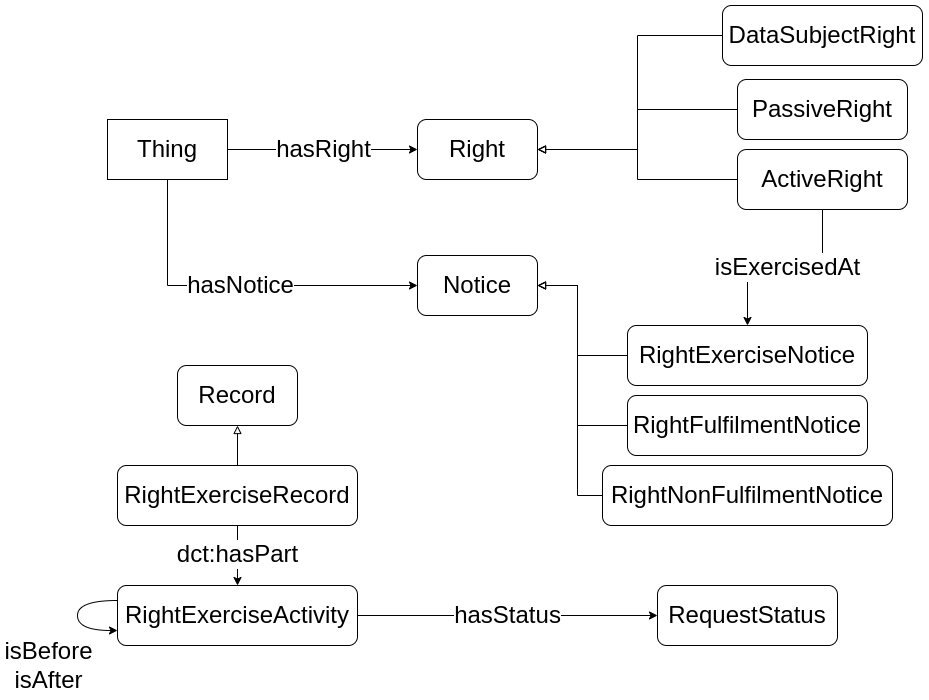
\includegraphics[width=0.8\linewidth]{figures/chapter-4/DPV-rights.png}
    \caption[Core concepts of DPV's rights taxonomy.]{Core concepts of DPV's rights taxonomy, adapted from \cite{pandit_primer_2022}.}
    \label{fig:rights_dpv}
\end{figure}

Thus, beyond modelling concepts for applicable \texttt{Right}s and \texttt{DataSubjectRight}s (applicable only to data subjects), to indicate the association of concepts with a particular right, the \texttt{hasRight} property is also modelled in DPV.
Additionally, to make a distinction between actionable and non-actionable rights, the \texttt{ActiveRight} and \texttt{PassiveRight} concepts were created to distinguish between rights that require an action to be taken for them to be exercised and rights that don't require any action and are always applicable.% add examples of active/passive rights
To fulfil the second objective of establishing where such active rights can be exercised, DPV's \texttt{isExercisedAt} property should be used to connect the right with the \texttt{RightExerciseNotice}.
This notice provides contextual information regarding how to exercise a right.
Specialised notice concepts for rights that can be fulfilled and those that cannot are modelled as \texttt{RightFulfilmentNotice} and \texttt{RightNonFulfilmentNotice}, respectively.

Moreover, to represent concrete records of rights being exercised, the \texttt{RightExerciseRecord} concept, specified as a subclass of DPV's \texttt{Record}, can be used to associate a particular request, or even distinct requests from the same data subject, with corresponding rights exercising activities, modelled as \texttt{RightExerciseActivity}, using the DCMI Metadata Terms \texttt{hasPart} property.
Such activity instances should include metadata, e.g., timestamps, duration, or involved entities, to track the provenance of a particular right exercising process, from the request itself to its acknowledgement by the data controller and to the fulfilment or non-fulfilment of the right.

In order to justify a certain right exercise activity, a collection of justifications for the non-fulfilment, i.e., \texttt{RightNonFulfilmentJustification}, delay of fulfilment, i.e.,\linebreak \texttt{RightFulfilmentDelayJustification}, and exercise of rights, i.e.,\linebreak \texttt{RightExerciseJustification}, were modelled as subclasses of the\linebreak \texttt{NonPerformanceJustification}, \texttt{DelayJustification}, and\linebreak \texttt{ExerciseJustification} concepts, which were modelled to have generic justification concepts that can be used beyond the rights domain.
\texttt{NotRequiredJustification}s are also modelled for when a certain request is not required as it does not apply. 
Figure~\ref{fig:justifications} contains the modelled justifications -- they are modelled as generic justifications to be included in DPV, which are then extended in DPV-GDPR by referencing specific GDPR clauses.
Moreover, the \texttt{dcterms:source} property will be used to connect the justification term with the GDPR provision that inspired its definition. 
These concepts have already been approved to be integrated into DPV and DPV-GDPR's outputs\footnote{Meeting notes of the DPVCG call where the concepts were accepted: \url{https://w3id.org/dpv/meetings/meeting-2024-03-13}.}.

\begin{figure}[ht]
    \centering
    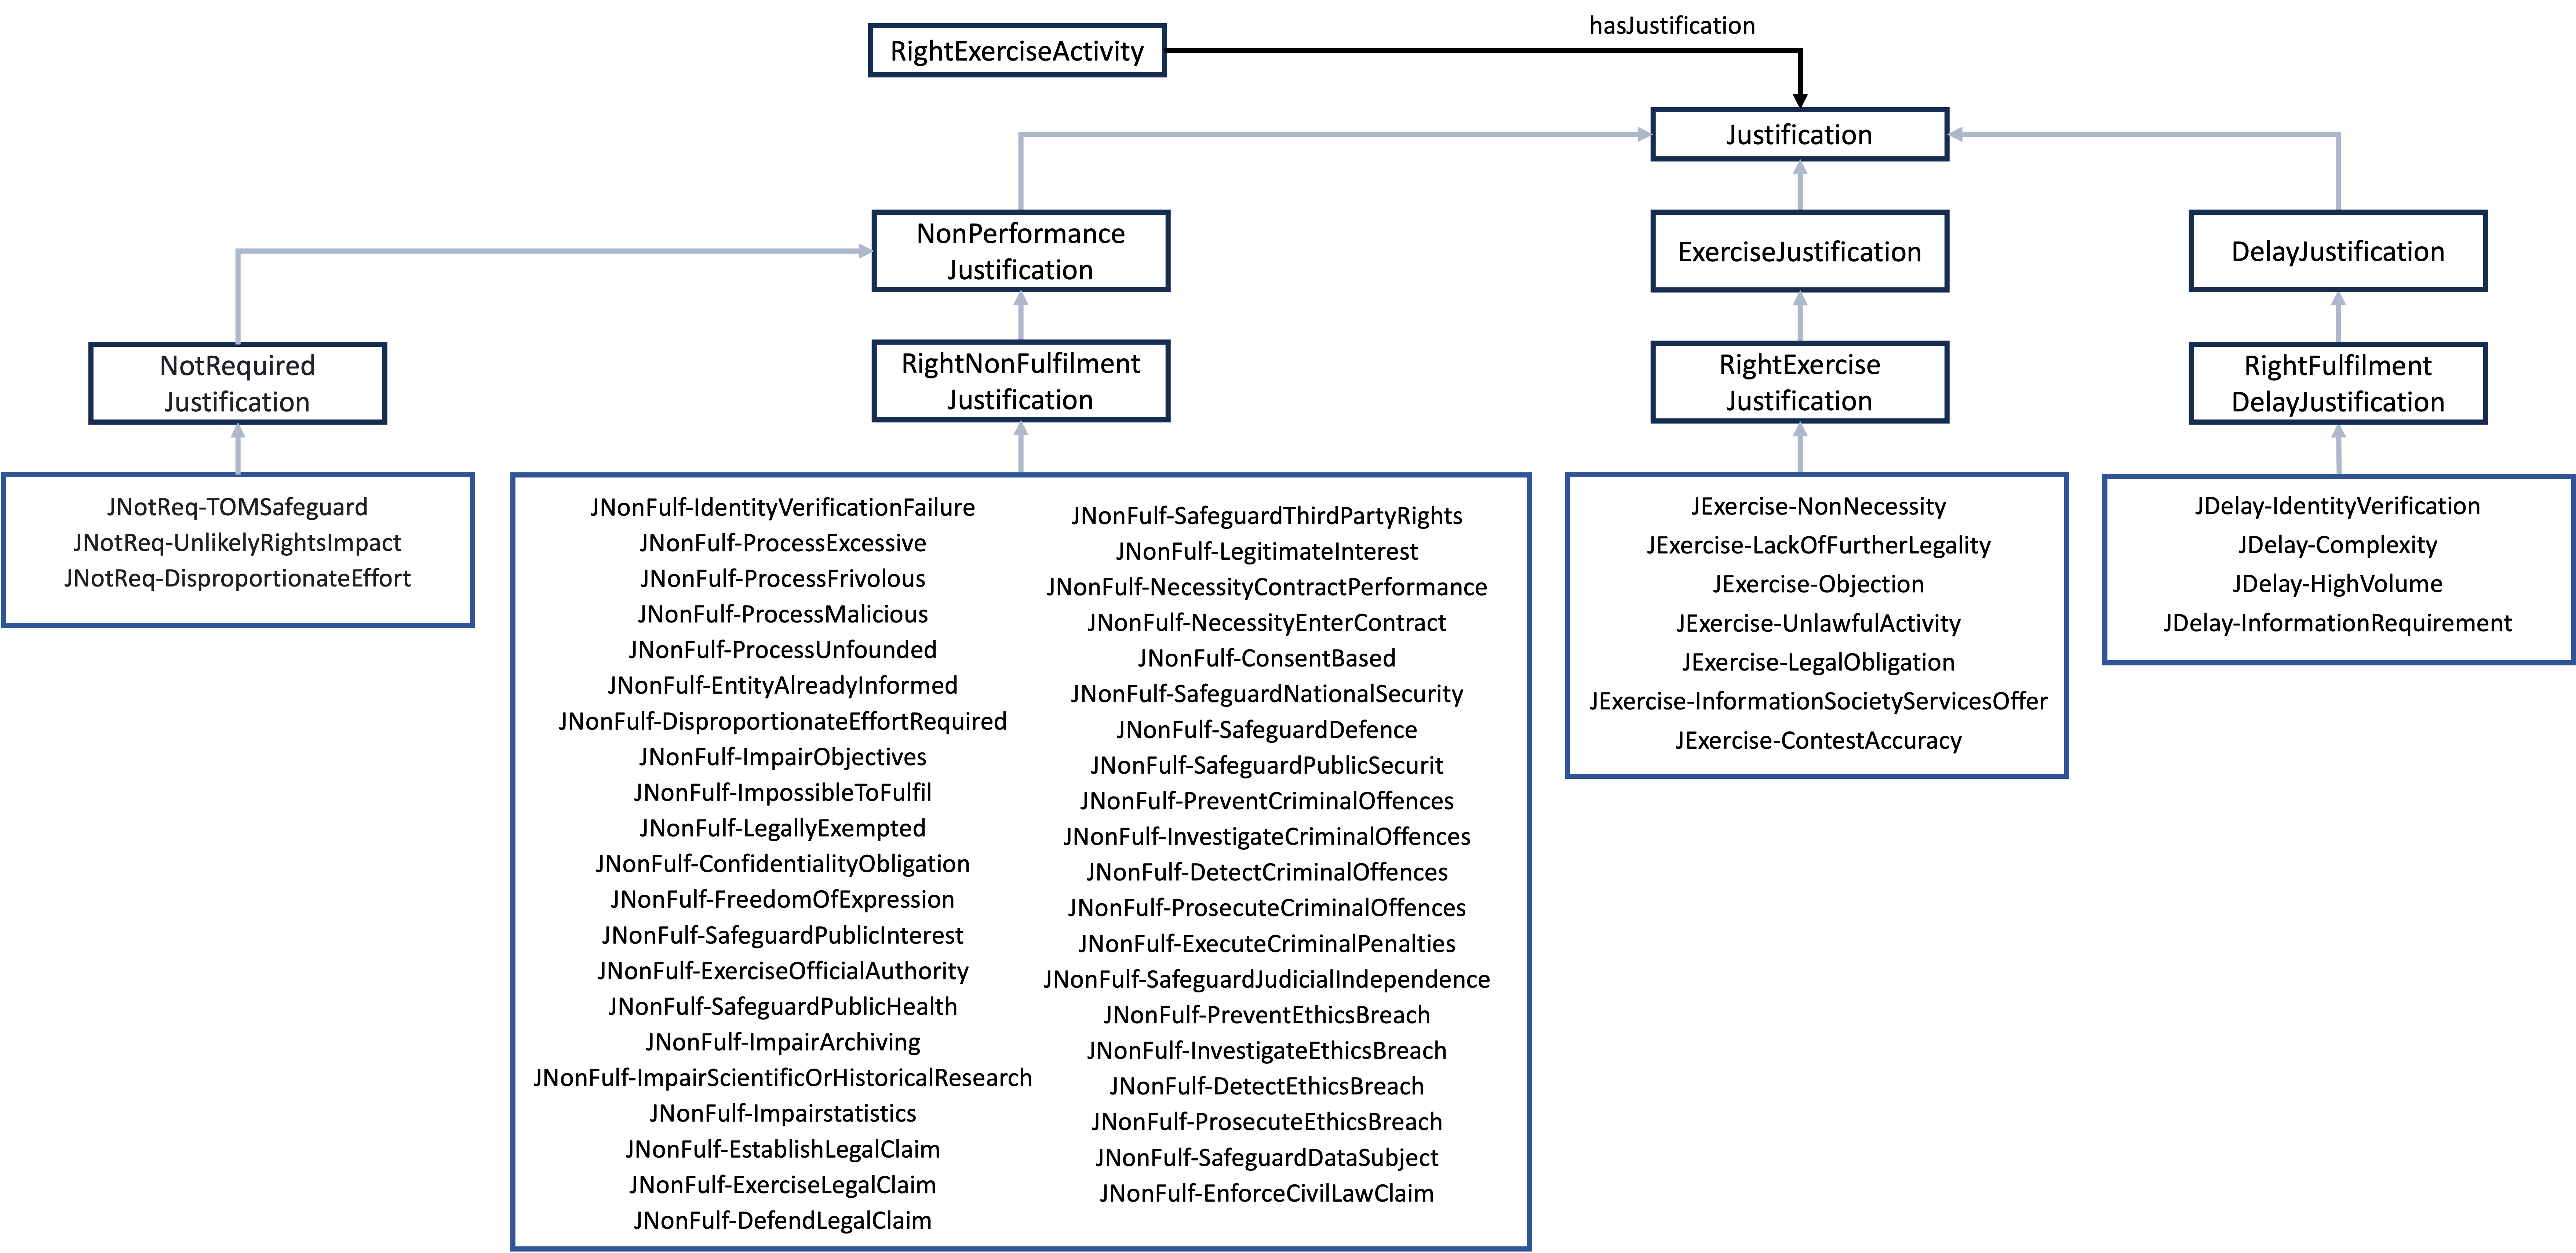
\includegraphics[width=\linewidth]{figures/chapter-4/justifications.png}
    \caption[Justification concepts.]{Justification concepts for the non-fulfilment, delay of fulfilment and exercise of rights.}
    \label{fig:justifications}
\end{figure}

Additionally, to track the status of rights exercising activities, a set of request statuses are modelled in DPV, including \texttt{RequestAccepted} for a request being accepted towards fulfilment, \texttt{RequestRejected} for a request being rejected towards non-fulfilment or\linebreak \texttt{RequestRequiresAction} for a request requiring an action to be performed from another party, and the \texttt{isBefore} and \texttt{isAfter} concepts can be used to specify that a specific activity occurs before or after another activity.

While this modelling was inspired by the GDPR, the concepts are described in a jurisdiction-agnostic manner so that they can be used to tackle data protection regulations in different jurisdictions.
For GDPR-specific rights, the \texttt{DataSubjectRight} concept is extended in DPV-GDPR with the data subject rights described in GDPR's Articles 13 to 22, as well as the rights to withdraw consent and to lodge a complaint with a supervisory authority, described in Articles 7.3 and 77.
Moreover, notices for direct and indirect data collection, to fulfil the information requirements in Articles 13 and 14, for Subject Access Requests (SARs), described in Article 15, and for notifying recipients, necessary to fulfil the communication requirements of Articles 16, 17 and 18, are provided as GDPR-specific subclasses of \texttt{RightFulfilmentNotice}s.

An overview of the aforementioned requirements and the intended purpose for modelling these concepts is presented in the ORSD illustrated in Table~\ref{tab:rights_ORSD}.

% also with these questions(in the ORSD) can you link directly to gdpr articles or other literature of gdpr implementation that help indicate these are valid requirements?

\begin{table}[htbp]
\centering
\caption{ORSD of the proposed model to express rights-related activities.}
\label{tab:rights_ORSD}
\scriptsize
\resizebox{\textwidth}{!}{%
\begin{tabular}{| l | l | l | l  | l | l | l |l| }
\hline
\multicolumn{8}{|c|}{\cellcolor[HTML]{A0A0A0}\textbf{Vocabulary-based patterns for rights exercising activities}} \\ \hline
\multicolumn{8}{|c|}{\cellcolor[HTML]{EFEFEF}\textbf{1. Purpose}} \\ \hline
\multicolumn{8}{| p{12.0cm} |}{The purpose of this model is the expression of rights-related activities, in particular focusing on data subject rights, such as the ones described in GDPR's Chapter III.} \\ \hline
\multicolumn{8}{|c|}{\cellcolor[HTML]{EFEFEF}\textbf{2. Scope}} \\ \hline
\multicolumn{8}{| p{12.0cm} |}{The scope of this model is limited to the expression of information related to the various steps of exercising data subject rights. In particular, the introduced concepts serve one of these purposes: (i) indicate what rights exist, (ii) express where such rights can be exercised, and (iii) record information related to concrete instances of rights that are being or were exercised. } \\ \hline
\multicolumn{8}{|c|}{\cellcolor[HTML]{EFEFEF}\textbf{3. Implementation Language}} \\ \hline
\multicolumn{8}{| p{12.0cm} |}{RDF, RDFS} \\ \hline
\multicolumn{8}{|c|}{\cellcolor[HTML]{EFEFEF}\textbf{4. Intended End-Users}} \\ \hline
\multicolumn{8}{| p{12.0cm} |}{Developers of Web services and applications, including decentralised storage solutions, that handle personal data.} \\ \hline
\multicolumn{8}{|c|}{\cellcolor[HTML]{EFEFEF}\textbf{5. Intended Uses}} \\ \hline
\multicolumn{8}{| p{12.0cm} |}{
Use 1. Declaration of the existence of data subject rights when the usage and collection of personal data is performed by Web services providers and developers, including information on where they can be exercised. \newline
Use 2. Patterns for data subject rights that can be fulfilled. \newline
Use 3. Patterns for data subject rights that cannot be fulfilled, including justifications for non-fulfilment. \newline
Use 4. Fulfilment of data subject rights requests from specific data protection legislation, such as the GDPR.
 } \\ \hline
\multicolumn{8}{|c|}{\cellcolor[HTML]{EFEFEF}\textbf{6. Ontology Requirements}} \\ \hline
\multicolumn{8}{|c|}{\cellcolor[HTML]{EFEFEF}\textbf{a. Non-Functional Requirements}}    \\ \hline
\multicolumn{8}{| p{12.0cm} |}{
NFR 1. The concepts are either published online within DPVCG's outputs, following W3C's specification format, or are under discussion for being adopted by the same CG. } \\ \hline
\multicolumn{8}{|c|}{\cellcolor[HTML]{EFEFEF}\textbf{b. Functional  Requirements: Groups of Competency Questions}}  \\ \hline
\multicolumn{5}{|c|}{\cellcolor[HTML]{EFEFEF}CQRG1. Related to data subject rights} & \multicolumn{3}{|c|}{\cellcolor[HTML]{EFEFEF}CQRG2. Related to GDPR} \\ \hline
\multicolumn{5}{ | m{7cm} |}{
CQR1. What rights are applicable in a given context? \newline
CQR2. Where can the right be exercised? \newline
CQR3. How can the right be exercised? \newline
CQR4. What data is necessary to implement the right? \newline 
CQR5. Which entity implements the right? \newline 
CQR6. Which entity exercised the right? \newline 
CQR7. When is the exercising activity occurring? \newline 
CQR8. What is the status of the right request? } & 
\multicolumn{3}{ m{5cm} |}{
CQR9. Which data subject rights are applicable according to the legal basis used by the data controller? \newline
CQR10. Which provenance metadata must controllers provide when replying to data subject rights requests? \newline 
CQR11. Which justification can be provided to not fulfil, delay or exercise a request?
}\\ \hline
\end{tabular}}
\vspace{-0.1in}
\end{table}

\subsection{Vocabulary-based patterns for rights exercising activities}
\label{sec:rights_patterns}

This Section outlines the usage of DPV for the expression of rights exercising activities, specifically related to the data subject rights described in GDPR's Chapter III.
Accordingly, the \textit{``controller shall take appropriate measures to provide any information referred to in Articles 13 and 14 and any communication under Articles 15 to 22 [...] to the data subject in a concise, transparent, intelligible and easily accessible form''} and if \textit{``the data subject makes the request by electronic form means, the information shall be provided by electronic means where possible, unless otherwise requested by the data subject''} \citeyearpar{noauthor_regulation_2016}.
Consequently, in this Thesis, personal data processing-related vocabularies such as DPV, and other semantic metadata vocabularies such as DCMI Metadata Terms and DCAT, are used for the establishment of structured notices and records of activities, which promote the fulfilment of the transparency and machine-readability requirements previously described.
Additionally, by storing such information in decentralised personal datastores, the accessibility requirement can also be satisfied.

Listing~\ref{list:applicable_rights} provides an example of a personal data handling activity, which can be used to express information regarding the what, how, where, who, and why personal data is being processed, as well as what rights exist.
The example provides information regarding the type of personal data, \texttt{pd:EmailAddress}, being processed by the \texttt{ex:DataController}, the purpose and legal basis used for the processing to occur, \texttt{dpv:ServiceProvision} and \texttt{eu-gdpr:A6-1-a}, and the applicable GDPR data subject rights.
This pattern can be followed by data controllers to express which rights are applicable, including rights beyond the ones in the GDPR, e.g., EU's fundamental rights and the rights depicted in other EU regulations or in other jurisdictions.

\begin{listing}[htp]
\caption[Personal data handling activity with applicable rights.]{Personal data handling activity example which includes information regarding the applicable rights.}
\label{list:applicable_rights}
\begin{minted}{turtle}
ex:ProcessEmailForServiceProvision a dpv:PersonalDataHandling ;
    dpv:hasDataController ex:DataController ;
    dpv:hasPersonalData pd:EmailAddress ;
    dpv:hasProcessing dpv:Collect, dpv:Use ;
    dpv:hasPurpose dpv:ServiceProvision ;
    dpv:hasLegalBasis eu-gdpr:A6-1-a ;
    dpv:hasRight eu-gdpr:A7-3, eu-gdpr:A13, eu-gdpr:A14, eu-gdpr:A15, eu-gdpr:A16, eu-gdpr:A17, eu-gdpr:A18, eu-gdpr:A20, eu-gdpr:A22, eu-gdpr:A77 .
ex:DataController a dpv:DataController .
\end{minted}
\end{listing}

Moreover, such declarations of applicable rights should include a notice of where they can be exercised.
Thus, as described in the previous Section, DPV’s \texttt{isExercisedAt} property should be used to connect rights with information on where to exercise it.
Such information should be provided through a \texttt{RightExerciseNotice}, along with other rights exercising metadata.

Listing~\ref{list:exercise_point} provides a notice with information on where to exercise the GDPR's right of access related to personal data being processed by the \texttt{ex:DataController}.
This notice uses the \texttt{dpv:hasRight} property to indicate which rights can be exercised, beyond the already mentioned access right, and the \texttt{foaf:page} property to express the precise Web page where the right can be exercised.
Additionally, DPV's \texttt{hasDataController} and\linebreak \texttt{isImplementedByEntity} properties are used to define who is the controller responsible for the personal data being processed and who is the entity implementing the service/platform where the rights are exercised -- in most cases this entity will probably coincide with the data controller, however, for transparency and accountability purposes, it is reasonable to express both terms.
Other entity-related properties can also be used to personalise the notice, e.g., if a notice is personalised for a specific data subject, then \texttt{dpv:hasDataSubject} can be used to connect the notice with the individual data subject. 
Furthermore, personal data handling instances can also be used to express `data processing bundles' that need to be provided in order to fulfil the data subjects' rights.
As previously mentioned, this can be done using DPV's taxonomies of purposes, personal data categories, processing operations, etc, e.g., in Listing~\ref{list:exercise_point}, an account identifier is required by the data controller for identity verification purposes in order to fulfil the data subject's rights described in GDPR's Articles 7.3, 15, 16, 17 and 20.
Other information might be needed to be communicated to the user, for instance, information on payments as Article 12.5(a) states that a fee \textit{``taking into account the administrative costs of providing the information or communication or taking the action requested''} might be requested by the data controller in case the data subject's request is unfounded, excessive or repetitive.
Such information can also be expressed in personal data handling instances including ODRL policies with duties constrained with an \texttt{odrl:payAmount} left operand.
% need to be provided / are being provided

\begin{listing}[htp]
\caption[GDPR Article 15's right of access exercise notice.]{GDPR Article 15's right of access exercise notice, including information on where to exercise the right and on necessary data to fulfil the right.}
\label{list:exercise_point}
\begin{minted}{turtle}
ex:RightToAccess a eu-gdpr:A15 ;
    dpv:isExercisedAt ex:RightExercisePoint .

ex:RightExercisePoint a dpv:RightExerciseNotice ;
    dpv:hasRight eu-gdpr:A7-3, eu-gdpr:A15, eu-gdpr:A16, eu-gdpr:A17, eu-gdpr:A20 ;
    dpv:hasDataController ex:DataController ;
    dpv:isImplementedByEntity ex:DataController ;
    foaf:page <https://example.com/DataController/RightExercisePoint> ;
    dpv:hasPersonalDataHandling [ 
        a dpv:PersonalDataHandling ;
        dpv:hasPurpose dpv:IdentityVerification ;
        dpv:hasPersonalData pd:AccountIdentifier ;
        dpv:hasProcessing dpv:Collect, dpv:Store ;
        dpv:hasRecipientDataController ex:DataController ] .
\end{minted}
\end{listing}

In addition to notices expressing what rights are applicable and where they can be exercised, provenance metadata must be kept when actual instances of the rights are exercised, throughout the whole process, from initiating a request to rejecting or fulfilling it.
As such, DPV's \texttt{RightExerciseActivity} can be used in conjunction with the W3C's PROV-O recommendation~\citep{lebo_prov-o_2013} to track the provenance of a right exercising activity instance.
Using this standard, provenance information, regarding the entities whom the request is associated with, i.e., \texttt{prov:wasAssociatedWith}, or what data/notice was generated, i.e., \texttt{prov:generated}, by the right exercise activity, can be represented.
\texttt{prov:actedOnBehalfOf} can also be used to represent delegation or representation, for instance when a parent exercises a right on behalf of its child.
Temporal information, descriptions and identifiers of the activities and their creators/publishers can be recorded using DCMI Metadata Terms.
Connections to the previous or following activities can be done using the \texttt{dpv:isAfter} and \texttt{dpv:isBefore} concepts, respectively.
Moreover, to track the status of a right exercising activity, DPV's taxonomy of request statuses concepts can be used.

Figure~\ref{fig:request_status} illustrates the sequence in which these concepts occur.
Once the request is initiated, it should be then acknowledged by the entity implementing it and either accepted towards fulfilment or rejected towards non-fulfilment.
Additionally, after being rejected, the entity fulfilling the request can also require further action from the requester (e.g., request additional data to be able to fulfil the request), which can delay the acceptance or rejection of the request, and after the required action is performed, the request can either be accepted towards fulfilment or get rejected again towards non-fulfilment or towards asking again for further action.

% perhaps formalise the semantics a bit more using uml state machine notation?
\begin{figure}[htp]
    \centering
    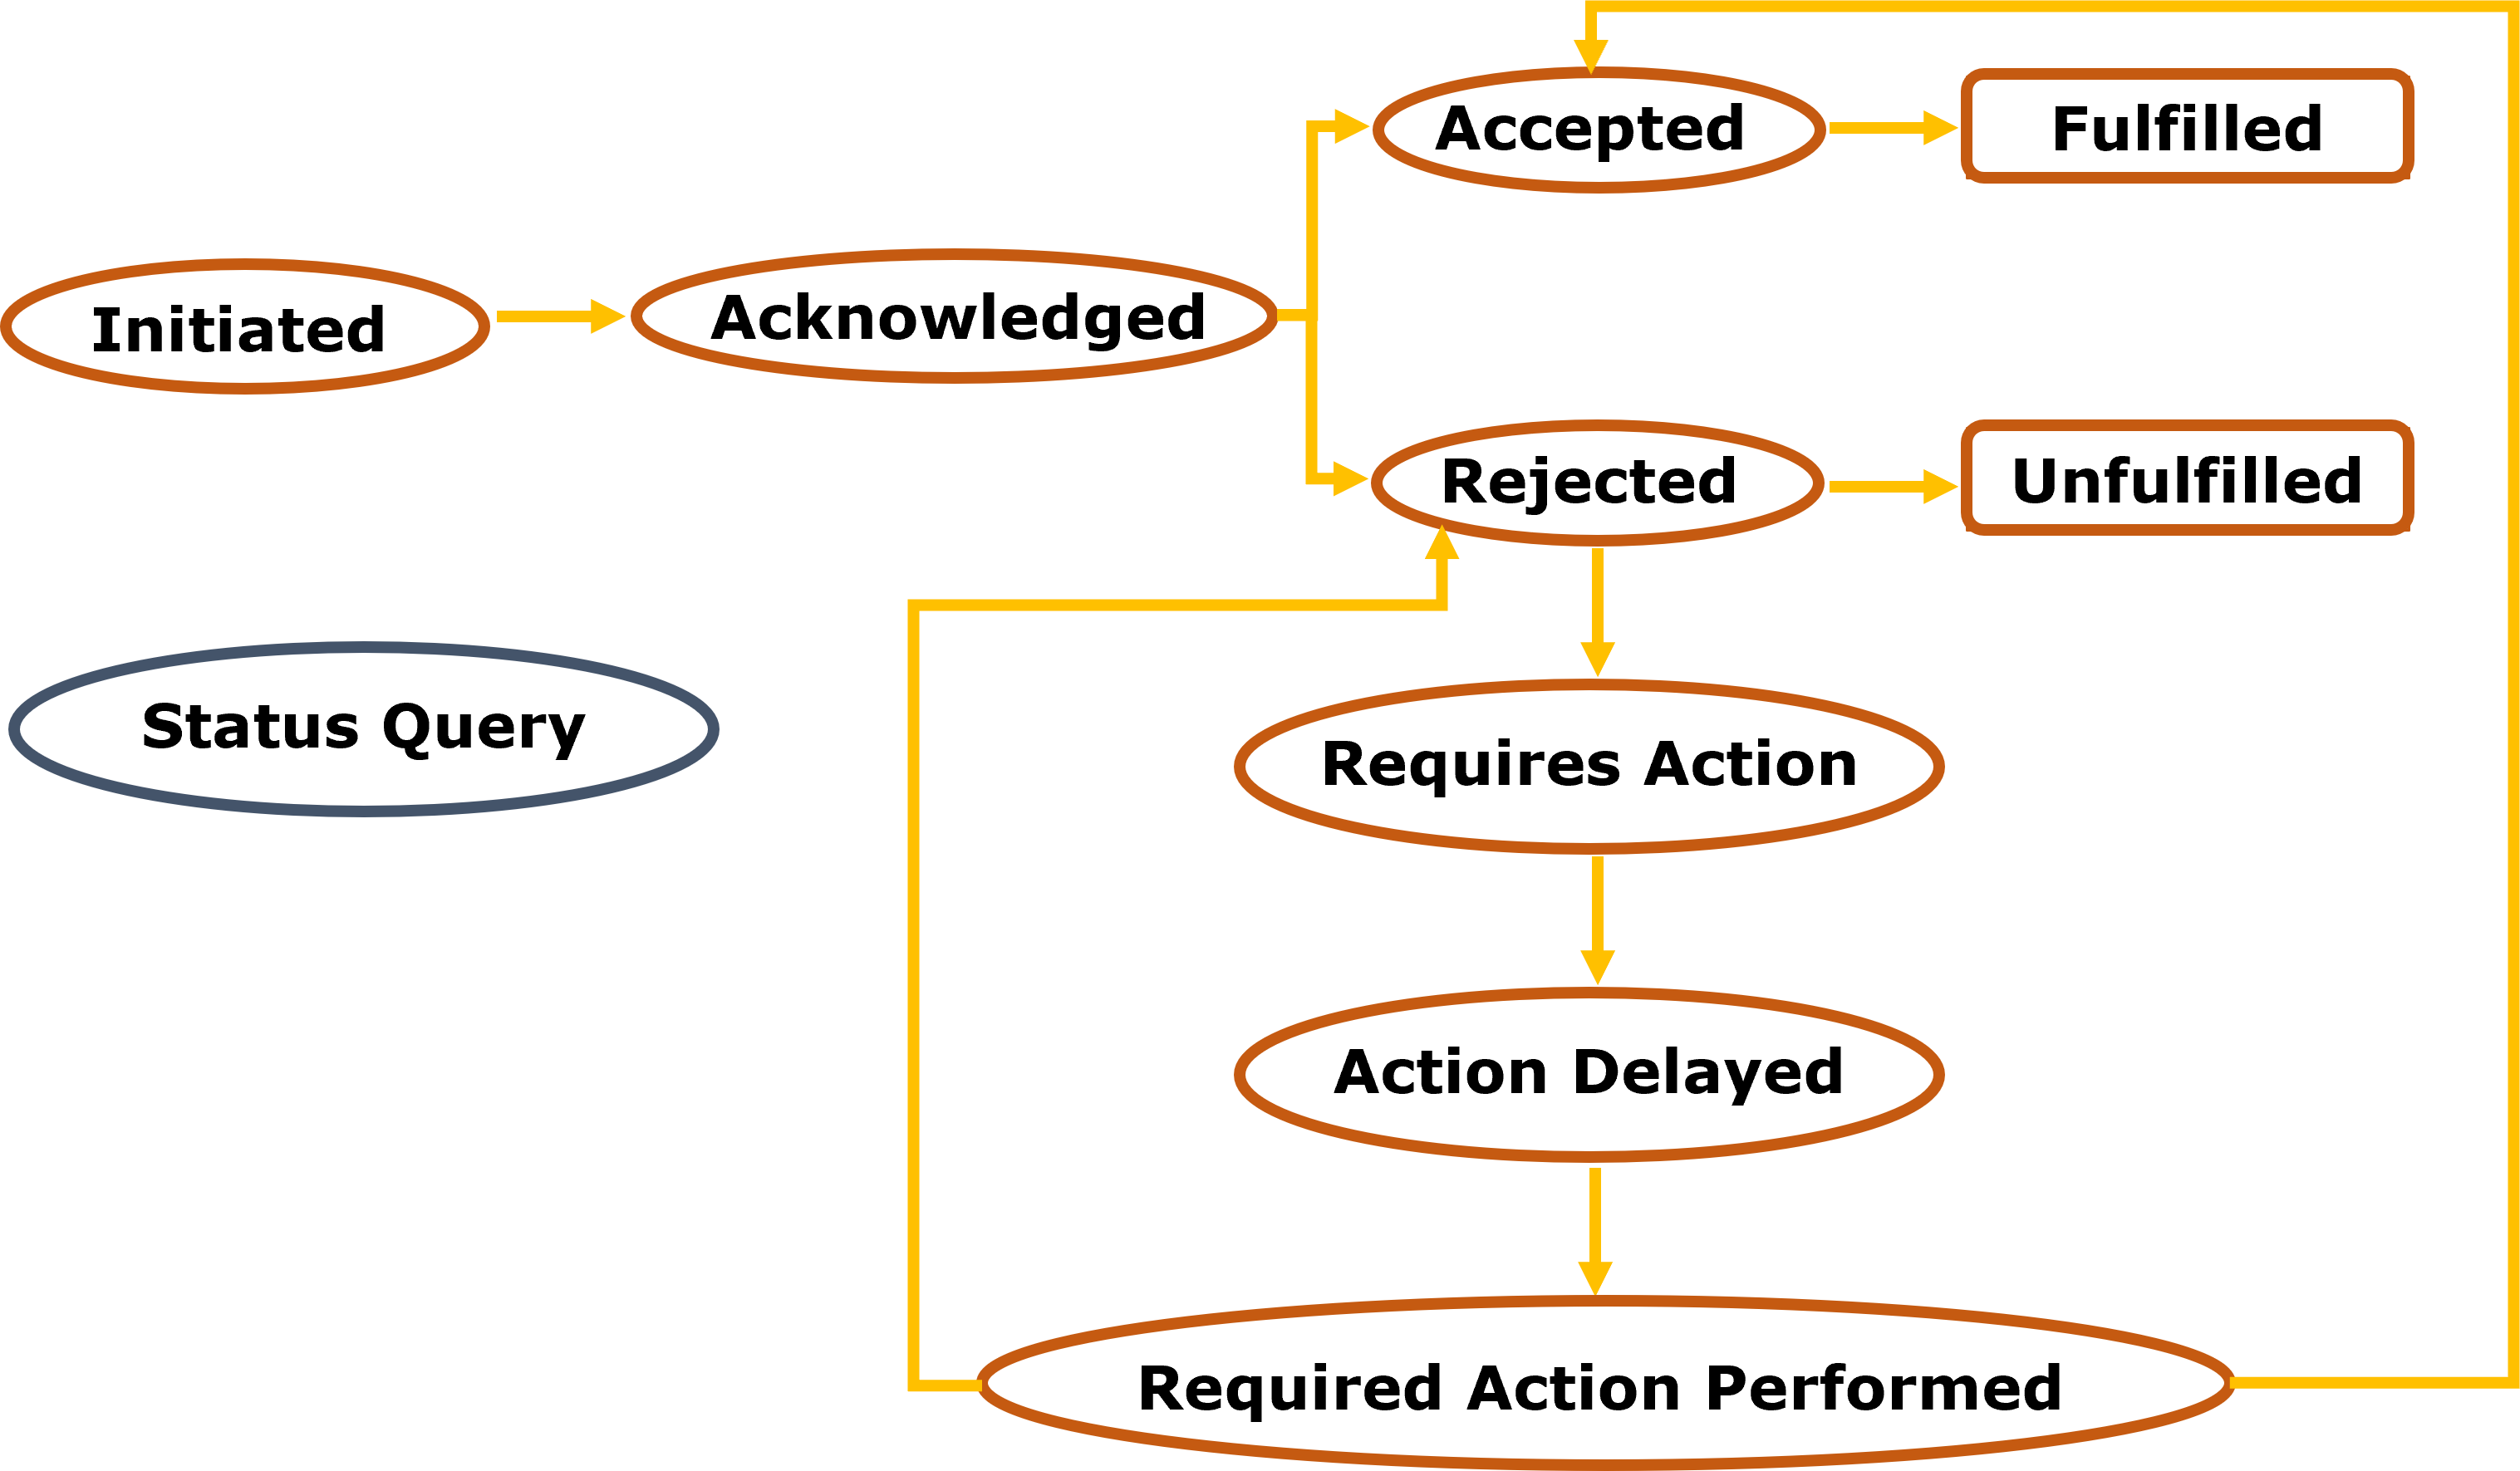
\includegraphics[width=0.8\linewidth]{figures/chapter-4/request-status.png}
    \caption{DPV's concepts to model the status of a request.}
    \label{fig:request_status}
\end{figure}

Listing~\ref{list:request_acknowledgment} illustrates a record of the right exercising activities related to a GDPR right of access request and acknowledgement of said request.
The activity associated with the start of the request has the status \texttt{dpv:RequestInitiated}, the data subject is identified using the \texttt{dpv:hasDataSubject} and the recipient of the request, a data controller, using the \texttt{dpv:hasRecipientDataController}.
Furthermore, a personal data handling instance can be used to express what personal data needs to be processed for the fulfilment of the right and DPV's \texttt{hasScope} to specify the scope of the request, e.g., the data subject only wants to access data processed for service provision purposes or only data processed during 2022.
Following the start of the request, the controller acknowledges the request, a right exercising activity which has \texttt{dpv:RequestAcknowledged} status and the recipient is the data subject that initiated the request.

\begin{listing}[htp]
\caption{Record of GDPR right of access request and acknowledgement activities.}
\label{list:request_acknowledgment}
\begin{minted}{turtle}
ex:DataSubject a dpv:DataSubject .
ex:DataSubjectUsername a pd:AccountIdentifier ;
    dpv:hasDataSubject ex:DataSubject .

ex:SARequest a dpv:RightExerciseActivity, prov:Activity ;
    dcterms:description "Data Subject makes a GDPR right of access request" ;
    dpv:hasRight eu-gdpr:A15 ;
    dpv:isExercisedAt ex:RightExercisePoint ;
    prov:wasAssociatedWith ex:DataSubject ;
    dpv:hasDataSubject ex:DataSubject ;
    dpv:hasRecipientDataController ex:DataController ;
    dcterms:date "2023-11-02T11:08:05"^^xsd:dateTime ;
    dpv:hasStatus dpv:RequestInitiated ;
    dpv:hasPersonalDataHandling [
        a dpv:PersonalDataHandling ;
        dpv:hasPurpose dpv:IdentityVerification ;
        dpv:hasPersonalData ex:DataSubjectUsername ;
        dpv:hasProcessing dpv:Collect, dpv:Store ] ;
    dpv:hasScope [
        dpv:hasPurpose dpv:ServiceProvision ;
        dpv:hasDuration [
            time:hasBeginning "2022-01-01T00:00:00"^^xsd:dateTime ;
            time:hasEnd "2022-12-31T23:59:59"^^xsd:dateTime ] ] .

ex:SARAcknowledged a dpv:RightExerciseActivity, prov:Activity ;
    dcterms:description "Data controller acknowledges the request" ;
    dcterms:date "2023-11-02T15:55:10"^^xsd:dateTime ;
    prov:wasAssociatedWith ex:DataController ;
    dpv:hasRecipient ex:DataSubjectUsername ;
    dpv:hasStatus dpv:RequestAcknowledged ;
    dpv:isAfter ex:SARequest .
\end{minted}
\end{listing}

Listing~\ref{list:further_action} illustrates the follow-up to Listing~\ref{list:request_acknowledgment} -- the request was rejected\linebreak due to the data controller not being able to identify the data subject,\linebreak \texttt{JNonFulf-IdentityVerificationFailure}.
Table~\ref{tab:justifications} contains the list of modelled right non-fulfilment justifications and their labels, which can be used by controllers for the purpose of justifying such requests.
As such the data controller requires further information from the data subject to be able to proceed with the request.
Such right exercise activity is identified with the \texttt{dpv:RequestRequiresAction} status and contains a personal data handling activity instance expressing the information that the data subject needs to provide for the right exercise to continue.
Afterwards, a right exercise activity associated with the data subject and with a \texttt{dpv:RequestRequiredActionPerformed} status is recorded with the information that the data subject provided.

\begin{listing}[htp]
\caption[Record requesting further information to fulfil SAR.]{Record of data controller requesting further information to fulfil the data subject's SAR and of the data subject providing the controller with said information.}
\label{list:further_action}
\begin{minted}{turtle}
ex:SARRejected a dpv:RightExerciseActivity, prov:Activity;
    dcterms:description "Data controller rejects the request" ;
    dcterms:date "2023-11-02T15:57:31"^^xsd:dateTime ;
    prov:wasAssociatedWith ex:DataController ;
    dpv:hasRecipient ex:DataSubjectUsername ;
    dpv:hasStatus dpv:RequestRejected ;
    dpv:hasJustification justif:JNonFulf-IdentityVerificationFailure ;
    dpv:isAfter ex:SARAcknowledged .

ex:SARRequiresAction a dpv:RightExerciseActivity, prov:Activity ;
    dcterms:description "Data controller requires further actions" ;
    dcterms:date "2023-11-02T16:09:21"^^xsd:dateTime ;
    prov:wasAssociatedWith ex:DataController ;
    dpv:hasRecipient ex:DataSubjectUsername ;
    dpv:hasStatus dpv:RequestRequiresAction ;
    dpv:hasJustification justif:JNonFulf-IdentityVerificationFailure ;
    dpv:hasPersonalDataHandling [
        dpv:hasPersonalData pd:OfficialID ;
        dpv:hasProcessing dpv:MakeAvailable ;
        dpv:hasPurpose dpv:IdentityVerification ;
        dpv:hasRecipientDataController ex:DataController ;
        dpv:isImplementedByEntity ex:DataSubjectUsername ] ;
    dpv:isAfter ex:SARRejected .

ex:DataSubjectOfficialID a pd:OfficialID ;
    dpv:hasDataSubject ex:DataSubject .

ex:SARActionPerformed a dpv:RightExerciseActivity, prov:Activity ;
    dcterms:description "Data Subject provides required information" ;
    dcterms:date "2023-11-02T17:20:42"^^xsd:dateTime ;
    prov:wasAssociatedWith ex:DataSubject ;
    dpv:hasStatus dpv:RequestRequiredActionPerformed ;
    dpv:hasPersonalDataHandling [
        dpv:hasPersonalData ex:DataSubjectOfficialID ;
        dpv:hasProcessing dpv:MakeAvailable ;
        dpv:hasPurpose dpv:IdentityVerification ;
        dpv:hasRecipientDataController ex:DataController ;
        dpv:isImplementedByEntity ex:DataSubjectUsername ] ;
    dpv:isAfter ex:SARRequiresAction .
\end{minted}
\end{listing}

% rights non-fulfilment justifications issue: https://github.com/w3c/dpv/issues/63 & meeting minutes:https://www.w3.org/2022/10/19-dpvcg-minutes.html
\begin{landscape}
\begin{table}
    \centering
    \caption{Justifications for non-fulfilment of GDPR's data subject rights.}
    \label{tab:justifications}
    \resizebox{\textwidth}{!}{%
    \begin{tabular}{c|l|c}
        \textbf{Term} & \textbf{Label} & \multicolumn{1}{c}{\begin{tabular}[c]{@{}c@{}} \textbf{GDPR} \\ \textbf{Article(s)} \end{tabular}} \\
        \hline\hline
        \texttt{JNonFulf-IdentityVerificationFailure} & \multicolumn{1}{l|}{\begin{tabular}[l]{@{}l@{}} Justification that the process could not be fulfilled or was not successful\\ because identity verification failed \end{tabular}} & 12.2 \\
        \hline
        \texttt{JNonFulf-ProcessExcessive} & Request was excessive in scope & 12.5 \\
        \hline
        \texttt{JNonFulf-ProcessFrivolous} & Request was frivolous in scope & 12.5 \\
        \hline
        \texttt{JNonFulf-ProcessMalicious} & Request was malicious in scope & 12.5 \\
        \hline
        \texttt{JNonFulf-ProcessUnfounded} & Request was unfounded in scope & 12.5 \\
         \hline
        \texttt{JNonFulf-EntityAlreadyInformed} & \multicolumn{1}{l|}{\begin{tabular}[l]{@{}l@{}} Data subject already has been provided with this information \end{tabular}} & 13.4, 14.5(a) \\
         \hline
        \texttt{JNonFulf-ImpairObjectives} & Fulfilment would cause impairment to processing & 14.5(b) \\
        \hline     
        \texttt{JNonFulf-DisproportionateEffortRequired} & Fulfilment would require extraordinary effort & 14.5(b), 19 \\
         \hline
        \texttt{JNonFulf-ImpossibleToFulfil} & Fulfilment would be impossible & 14.5(b), 19 \\
         \hline
        \texttt{JNonFulf-LegallyExempted} & \multicolumn{1}{l|}{\begin{tabular}[l]{@{}l@{}} Fulfilment not needed as it falls under legal exemption \end{tabular}} & \multicolumn{1}{l}{\begin{tabular}[l]{@{}l@{}} 14.5(c), 17.3(b),\\ 22.2(b) \end{tabular}} \\
         \hline
        \texttt{JNonFulf-ConfidentialityObligation} & \multicolumn{1}{l|}{\begin{tabular}[l]{@{}l@{}} Fulfilment would compromise existing confidentiality obligations \end{tabular}} & 14.5(d) \\
        \hline
        \texttt{JNonFulf-FreedomOfExpression} & \multicolumn{1}{l|}{\begin{tabular}[l]{@{}l@{}} Fulfilment would interfere with the right of freedom of expression\\ and information of others \end{tabular}} & 17.3(a) \\
         \hline
        \texttt{JNonFulf-SafeguardPublicInterest} & \multicolumn{1}{l|}{\begin{tabular}[l]{@{}l@{}} Fulfilment would interfere with necessary tasks carried out for public\\ interest \end{tabular}} & \multicolumn{1}{l}{\begin{tabular}[l]{@{}l@{}} 17.3(b), 21.6,\\ 23.1(e) \end{tabular}} \\
         \hline
         \texttt{JNonFulf-ExerciseOfficialAuthority} & \multicolumn{1}{l|}{\begin{tabular}[l]{@{}l@{}} Fulfilment would interfere with the exercise of official authorities \end{tabular}} & \multicolumn{1}{l}{\begin{tabular}[l]{@{}l@{}} 17.3(b), 20.3,\\ 23.1(h) \end{tabular}} \\
         \hline
         \texttt{JNonFulf-SafeguardPublicHealth} & \multicolumn{1}{l|}{\begin{tabular}[l]{@{}l@{}} Fulfilment would interfere with necessary tasks carried out for public\\ health reasons \end{tabular}} & 17.3(c) \\
         \hline
        \texttt{JNonFulf-ImpairArchiving} & \multicolumn{1}{l|}{\begin{tabular}[l]{@{}l@{}} Fulfilment would compromise or hinder archiving purposes \end{tabular}} & 17.3(d) \\
        \hline
        \texttt{JNonFulf-ImpairScientificOrHistoricalResearch} & \multicolumn{1}{l|}{\begin{tabular}[l]{@{}l@{}} Fulfilment would impair scientific or historical research \end{tabular}} & 17.3(d) \\
        \hline
        \texttt{JNonFulf-ImpairStatistics} & \multicolumn{1}{l|}{\begin{tabular}[l]{@{}l@{}} Fulfilment would interfere with official statistics \end{tabular}} & 17.3(d) \\
        \hline
        \texttt{JNonFulf-EstablishLegalClaim} & \multicolumn{1}{l|}{\begin{tabular}[l]{@{}l@{}} Fulfilment would interfere with the establishment of legal claims \end{tabular}} & 17.3(e), 21.1 \\
        \hline
        \texttt{JNonFulf-ExerciseLegalClaim} & \multicolumn{1}{l|}{\begin{tabular}[l]{@{}l@{}} Fulfilment would interfere with the exercise of legal claims \end{tabular}} & 17.3(e), 21.1 \\
        \hline
        \texttt{JNonFulf-DefendLegalClaim} & \multicolumn{1}{l|}{\begin{tabular}[l]{@{}l@{}} Fulfilment would interfere with the defence of legal claims \end{tabular}} & 17.3(e), 21.1 \\
        \hline
        \texttt{JNonFulf-SafeguardThirdPartyRights} & \multicolumn{1}{l|}{\begin{tabular}[l]{@{}l@{}} Fulfilment would adversely affect the rights of other data subjects or third\\ parties \end{tabular}} & 20.4, 23.1(i) \\
         \hline
         \texttt{JNonFulf-LegitimateInterest} & \multicolumn{1}{l|}{\begin{tabular}[l]{@{}l@{}} Fulfilment would interfere with the legitimate interest of the controller\\ which overrides the interests or rights of the data subject \end{tabular}} & 21.1 \\
         \hline
        \texttt{JNonFulf-NecessityContractPerformance} & \multicolumn{1}{l|}{\begin{tabular}[l]{@{}l@{}} Fulfilment would interfere with the performance of a contract \end{tabular}} & 22.2(a) \\
         \hline
        \texttt{JNonFulf-NecessityEnterContract} & \multicolumn{1}{l|}{\begin{tabular}[l]{@{}l@{}} Fulfilment would interfere with the necessity of entering into a contract \end{tabular}} & 22.2(a) \\
         \hline
        \texttt{JNonFulf-ConsentBased} & \multicolumn{1}{l|}{\begin{tabular}[l]{@{}l@{}} Fulfilment not necessary as processing is based on explicit consent \end{tabular}} & 22.2(c) \\
        \hline
        \texttt{JNonFulf-SafeguardNationalSecurity} & \multicolumn{1}{l|}{\begin{tabular}[l]{@{}l@{}} Fulfilment would pose a threat to safeguard national security \end{tabular}} & 23.1(a) \\
         \hline
        \texttt{JNonFulf-SafeguardDefence} & Fulfilment would pose a threat to safeguard defence & 23.1(b) \\
         \hline
        \texttt{JNonFulf-SafeguardPublicSecurity} & \multicolumn{1}{l|}{\begin{tabular}[l]{@{}l@{}} Fulfilment would pose a threat to safeguard public security \end{tabular}} & 23.1(c) \\
         \hline
        \texttt{JNonFulf-PreventCriminalOffences} & \multicolumn{1}{l|}{\begin{tabular}[l]{@{}l@{}} Fulfilment would interfere with the prevention of criminal offences \end{tabular}} & 23.1(d) \\
        \hline
        \texttt{JNonFulf-InvestigateCriminalOffences} & \multicolumn{1}{l|}{\begin{tabular}[l]{@{}l@{}} Fulfilment would interfere with the investigation of criminal offences \end{tabular}} & 23.1(d) \\
        \hline
        \texttt{JNonFulf-DetectCriminalOffences} & \multicolumn{1}{l|}{\begin{tabular}[l]{@{}l@{}} Fulfilment would interfere with the detection of criminal offences \end{tabular}} & 23.1(d) \\
        \hline
        \texttt{JNonFulf-ProsecuteCriminalOffences} & \multicolumn{1}{l|}{\begin{tabular}[l]{@{}l@{}} Fulfilment would interfere with the prosecution of criminal offences \end{tabular}} & 23.1(d) \\
        \hline
        \texttt{JNonFulf-ExecuteCriminalPenalties} & \multicolumn{1}{l|}{\begin{tabular}[l]{@{}l@{}} Fulfilment would interfere with the execution of criminal penalties \end{tabular}} & 23.1(d) \\
        \hline
        \texttt{JNonFulf-SafeguardJudicialIndependence} & \multicolumn{1}{l|}{\begin{tabular}[l]{@{}l@{}} Fulfilment would pose a threat to safeguard judicial independence or\\ proceedings \end{tabular}} & 23.1(f) \\
        \hline
        \texttt{JNonFulf-PreventEthicsBreach} & \multicolumn{1}{l|}{\begin{tabular}[l]{@{}l@{}} Fulfilment would interfere with the prevention of breaches of ethics for\\ regulated professions \end{tabular}} & 23.1(g) \\
        \hline
        \texttt{JNonFulf-InvestigateEthicsBreach} & \multicolumn{1}{l|}{\begin{tabular}[l]{@{}l@{}} Fulfilment would interfere with the investigation of breaches of ethics for\\ regulated professions \end{tabular}} & 23.1(g) \\
        \hline
        \texttt{JNonFulf-DetectEthicsBreach} & \multicolumn{1}{l|}{\begin{tabular}[l]{@{}l@{}} Fulfilment would interfere with the detection of breaches of ethics for\\ regulated professions \end{tabular}} & 23.1(g) \\
        \hline
        \texttt{JNonFulf-ProsecuteEthicsBreach} & \multicolumn{1}{l|}{\begin{tabular}[l]{@{}l@{}} Fulfilment would interfere with the prosecution of breaches of ethics for\\ regulated professions \end{tabular}} & 23.1(g) \\
        \hline
        \texttt{JNonFulf-SafeguardDataSubject} & \multicolumn{1}{l|}{\begin{tabular}[l]{@{}l@{}} Fulfilment would interfere with the protection of the data subject \end{tabular}} & 23.1(i) \\
         \hline
        \texttt{JNonFulf-EnforceCivilLawClaim} & Fulfilment would interfere with the enforcement of civil law claims & 23.1(j) \\
    \end{tabular}}
\end{table}
\end{landscape}
% Information is legally exempt from disclosure	- Documents that have personal data of the data subject exempt from disclosure in court proceedings apply in relation to a Subject Access Request, this applies to both legal advice and litigation privilege

Listing~\ref{list:sar_notice} illustrates the follow-up to Listing~\ref{list:further_action} -- the request was accepted and fulfilled by the data controller and as such the data controller provides the data subject with a notice of the fulfilment of GDPR's Art.15, modelled as a \texttt{eu-gdpr:SARNotice}, and a copy of the data whose access was requested, modelled as a \texttt{dcat:Dataset}.
Beyond temporal information and providing the location of the notice, a personal data handling instance can be used to provide additional information to the data subject -- in the case of this SAR notice, the data subject is also notified of the type of personal data being processed, the purpose for the processing, the time period when the data was processed and the additional data subject rights that can be exercised.

\begin{listing}[htp]
\caption[Record of the acceptance and fulfilment of a SAR request.]{Record of the acceptance and fulfilment of the request and respective \texttt{SARNotice}.}
\label{list:sar_notice}
\begin{minted}{turtle}
ex:SARAccepted a dpv:RightExerciseActivity, prov:Activity ;
    dcterms:description "Request accepted by data controller towards fulfilment" ;
    dcterms:date "2023-11-03T08:15:04"^^xsd:dateTime ;
    prov:wasAssociatedWith ex:DataController ;
    dpv:hasRecipient ex:DataSubjectUsername ;
    dpv:hasStatus dpv:RequestAccepted ;
    dpv:isAfter ex:SARActionPerformed .

ex:SARFulfilled a dpv:RightExerciseActivity, prov:Activity ;
    dcterms:description "Request fulfilled by data controller" ;
    dcterms:date "2023-11-03T08:37:25"^^xsd:dateTime ;
    prov:wasAssociatedWith ex:DataController ;
    dpv:hasRecipient ex:DataSubjectUsername ;
    dpv:hasStatus dpv:RequestFulfilled ;
    prov:generated ex:DataCopy, ex:SARNotice_Username ;
    dpv:isAfter ex:SARAccepted .

ex:SARNotice_Username a eu-gdpr:SARNotice ;
    dcterms:date "2023-11-03T08:31:51"^^xsd:dateTime ;
    foaf:page <https://example.com/DataController/SARNotice_Username> ;
    dpv:hasPersonalDataHandling [
        dpv:hasPersonalData pd:EmailAddress ;
        dpv:hasPurpose dpv:ServiceProvision ;
        dpv:hasDuration [
            time:hasBeginning "2022-01-01T00:00:00"^^xsd:dateTime ;
            time:hasEnd "2022-12-31T23:59:59"^^xsd:dateTime ] ;
        dpv:hasRight eu-gdpr:A16, eu-gdpr:A17, eu-gdpr:A18, eu-gdpr:A21, eu-gdpr:A77 ] .

ex:DataCopy a dcat:Dataset ;
    dcterms:format <https://www.iana.org/assignments/media-types/text/csv> ;
    dcterms:accessRights access-right:c_16ec ; # restricted access
    dcterms:issued "2023-11-03T08:35:42"^^xsd:dateTime ;
    dcterms:valid "2023-12-03T08:35:42"^^xsd:dateTime ;
    dcat:landingPage <https://example.com/Username/SAR_DataCopy> .
\end{minted}
\end{listing}

Moreover, DCAT \citep{albertoni_data_2020} can be used to model resources beyond notices, for instance, a copy of the personal data, in the case of a right of access request according to the GDPR, as in Listing~\ref{list:sar_notice}.
Information regarding the format, validity and dataset provision/download location can be attached to the dataset representation using the \texttt{dcterms:format}, \texttt{dcterms:valid} and \texttt{dcat:landingPage} properties, respectively.
Additionally, DCAT -- and also the Data on the Web Best Practices Recommendation~\citep{loscio_data_2017} -- promotes the usage of ODRL to express license and rights statements, by linking the dataset with an ODRL policy using the \texttt{odrl:hasPolicy} property, or the usage of DCMI Metadata Terms' \texttt{license}, \texttt{accessRights} or \texttt{rights} properties to link datasets with licenses, access rights statements or other types of rights statements, e.g., copyrights, respectively.
In the case of using the latter, controlled vocabularies such as COAR's Access Rights vocabulary~\citep{apollaro_controlled_2022}, used in Listing~\ref{list:sar_notice} to restrict access only to the data subject, or the Named Authority List of Access rights from the~\cite{publications_office_of_the_european_union_named_2023} can be used to express `high-level' access control statements, e.g., embargoed, restricted or open access.
As such, by using DCAT and a policy expression vocabulary, i.e., ODRL, the user can easily control the transition of a compliance log and respective metadata, as proposed in PLASMA, from being only accessible by the user to be accessible by external auditors.

In this Section, the GDPR's Right of Access is used as an example to showcase how to model notices and right exercising activities using DPV, DCMI Metadata Terms, PROV-O and DCAT.
However, a similar pattern can be followed by data controllers to fulfil the other rights as in most cases the only substantial change would be the notice concept that needs to be used for a particular right instance, e.g., \texttt{eu-gdpr:DirectDataCollectionNotice} for the right fulfilment notice related to GDPR's Article 13, \texttt{eu-gdpr:IndirectDataCollectionNotice} for the right fulfilment notice related to GDPR's Article 14 or \texttt{eu-gdpr:RightsRecipientsNotice} for the right fulfilment notice related to GDPR's Article 19.
Moreover, some GDPR rights, such as the right to erasure in Article 17 and the right to restriction of processing in Article 18, also require the data subject to provide a justification for their request to be fulfilled by the data controller.
As such, a collection of justifications for the exercise of data subject rights, extracted from the GDPR and illustrated in Table~\ref{tab:fulfil_justifications}, was also modelled (as subclasses of a high-level \texttt{RightExerciseJustification} concept). % and is already approved to be integrated into DPV-GDPR's outputs.


\begin{table}
    \centering
    \caption[Justifications for the exercise of GDPR's data subject rights]{Justifications for the exercise of GDPR's data subject rights.}
    \label{tab:fulfil_justifications}
    \resizebox{\textwidth}{!}{%
    \begin{tabular}{c|p{8.5cm}|c}
        \textbf{Term} & \textbf{Label} & \multicolumn{1}{c}{\begin{tabular}[c]{@{}c@{}} \textbf{GDPR} \\ \textbf{Article(s)} \end{tabular}} \\
        \hline\hline
        \texttt{JExercise-NonNecessity} & \multicolumn{1}{l|}{\begin{tabular}[l]{@{}l@{}} Processing no longer necessary for the \\specified purposes \end{tabular}} & \multicolumn{1}{l}{\begin{tabular}[l]{@{}l@{}} 17.1(a),\\ 18.1(c) \end{tabular}} \\
        \hline
        \texttt{JExercise-LackOfFurtherLegality} & \multicolumn{1}{l|}{\begin{tabular}[l]{@{}l@{}} Processing no longer necessary due to a lack of further\\ legality of the legal basis of specified context \end{tabular}} & 17.1(b) \\
        \hline
        \texttt{JExercise-Objection} & Data subject objected to the processing & \multicolumn{1}{l}{\begin{tabular}[l]{@{}l@{}} 17.1(c),\\ 18.1(d) \end{tabular}} \\
        \hline
        \texttt{JExercise-UnlawfulActivity} & Personal data unlawfully processed & \multicolumn{1}{l}{\begin{tabular}[l]{@{}l@{}} 17.1(d),\\ 18.1(b) \end{tabular}} \\
        \hline
        \texttt{JExercise-LegalObligation} & Compliance with a legal obligation & 17.1(e) \\
        \hline
        \texttt{JExercise-InformationSocietyServicesOffer} & \multicolumn{1}{l|}{\begin{tabular}[l]{@{}l@{}} Personal data collected in relation to the offer \\of information society services \end{tabular}} & 17.1(f) \\
        \hline
        \texttt{JExercise-ContestAccuracy} & \multicolumn{1}{l|}{\begin{tabular}[l]{@{}l@{}} Accuracy of personal data contested by the \\data subject \end{tabular}} & 18.1(a) \\
    \end{tabular}}
\end{table}

\subsection{Justifications publication and maintenance}
\label{sec:justifications_publication}

As discussed in the previous sections, most rights-related concepts were already proposed and are integrated into DPV and DPV-GDPR.
The justifications concepts have already been approved to be accepted, but are still to be published in DPVCG's outputs.
As such, the justifications vocabulary human-readable documentation and machine-readable file are available at \url{https://w3id.org/people/besteves/justifications} using content negotiation.
Once the justification terms are fully integrated into DPV, this documentation will be archived as the maintenance of the terms will be performed as part of the DPVCG's activities.

The HTML documentation includes a description of the defined terms, which was conducted and validated with domain experts\footnote{This validation was performed with legal and ontology engineering experts in the context of W3C's DPV community group.}, diagrams with graphical representations of the several taxonomies used in the vocabulary patterns specific in this section, and RDF examples that use the defined terms to express rights-related activities.
The vocabulary documentation also includes metadata, such as the identity of the creators and publishers of the ontology, the dates of creation and last modification or the version number.
The source code is hosted at \url{https://w3id.org/people/besteves/justifications/repo}, under the CC-BY-4.0 license.
The repository can also be used by implementers to suggest new inclusions to the vocabulary and to report bugs through GitHub Issues.

Additionally, an auxiliary webpage, openly available at \url{https://w3id.org/people/besteves/rights}, provides guidelines and further examples on how to use DPV and the developed \texttt{Justification} terms to model the vocabulary-based patterns for rights-related activities defined in this Section.
The source code is hosted at \url{https://w3id.org/people/besteves/rights/repo}, under the CC-BY-4.0 license.
% \section{Ontology quality evaluation}
\label{sec:evaluation}

This Section describes the results of the ontologies quality evaluation, including the detection of common pitfalls with OOPS!\footnote{The OOPS! tool is available at \url{https://oops.linkeddata.es/} (accessed on 14 June 2023).}~\citep{poveda-villalon_oops_2014}, alignment with FAIR principles with FOOPS!\footnote{The FOOPS! tool is available at \url{https://w3id.org/foops} (accessed on 30 November 2023).}~\citep{garijo_foops_2021} and validation of competency questions with SPARQL queries~\citep{harris_sparql_2013}.

In terms of quality evaluation, the OOPS! tool was used to evaluate PLASMA and OAC in order to detect common errors in ontology development, such as missing domain or range properties or missing human-readable annotations.
Both evaluations did not detect any critical (issues affecting the ontology consistency, reasoning, or applicability) or important (issues not critical for ontology functionality but that should be corrected) pitfalls.
Furthermore, FOOPS! was used to evaluate the alignment of the developed vocabularies with the FAIR (Findable, Accessible, Interoperable and Reusable) principles.
Additionally, the vocabularies that were reused in this Section, e.g., DPV, ODRL, or ActivityStreams, were also evaluated with FOOPS! for comparison.
Table~\ref{tab:foops_evaluation} presents the results of this evaluation.

\begin{table}[htp]
    \centering
    \caption{Evaluation of the alignment of the developed and reused vocabularies with FAIR principles using FOOPS!.}
    \label{tab:foops_evaluation}
    \resizebox{\textwidth}{!}{%
    \begin{tabular}{c||c|c|c|c|c}
        \textbf{Ontology} & \textbf{FOOPS! score} & \textbf{Findable} & \textbf{Accessible} & \textbf{Interoperable} & \textbf{Reusable} \\
        \hline\hline
        OAC & 91\% & 8/9 & 2/3 & 3/3 & 8.83/9 \\
        \hline
        PLASMA & 91\% & 8/9 & 2/3 & 3/3 & 8.83/9 \\
        \hline 
        DPV & 64\% & 5.33/9 & 2/3 & 3/3 & 4.92/9 \\
        \hline 
        ODRL & 64\% & 4.5/9 & 3/3 & 3/3 & 4.75/9 \\
        \hline
        DCAT & 64\% & 4.33/9 & 3/3 & 3/3 & 5.14/9 \\
        \hline
        ACP & 52\% & 5.33/9 & 2/3 & 2/3 & 3.12/9 \\
        \hline
        ActivityStreams & 19\% & 2/9 & 1.5/3 & 0/3 & 1/9 \\
        \hline 
        ACL & 2\% & 0/9 & 0.5/3 & 0/3 & 0/9 \\
        \hline
        DCMI & 2\% & 0/9 & 0.5/3 & 0/3 & 0/9 \\
    \end{tabular}}
\end{table}

Both PLASMA and OAC obtained a good score in all FAIR aspects.
In terms of improvements, both vocabularies will be submitted to LOV (Linked Open Vocabularies), a public registry of ontologies that includes ontology metadata related to its terms and the creators/developers of the ontologies~\citep{dumontier_linked_2017}.
This will improve both the findability and the accessibility of the vocabularies.
Using Table~\ref{tab:foops_evaluation}, it can be observed that both PLASMA and OAC rate much higher than other reused ontologies in terms of findability and reusability as the used URIs and version URIs are persistent and resolvable, both include the recommended ontology and ontology terms metadata, a resolvable data usage license and provenance metadata.

Additionally, SPARQL queries are used to assess whether the developed models satisfy the competency questions, presented in Tables~\ref{tab:OAC_ORSD}, \ref{tab:plasma_orsd} and \ref{tab:rights_ORSD}, which were used to guide the development of the vocabularies in order to fulfil the identified requirements.

Table~\ref{tab:oac_cq_sparql} presents the SPARQL queries drafted to fulfil OAC's competency questions presented in Table~\ref{tab:OAC_ORSD}.
The presented work demonstrates that OAC satisfies the identified requirements of answering competency questions regarding the modelling of policies representing personal preferences, requests of data for particular purposes, and agreements of data access, including contextual information.
In particular, these competency questions showcase OAC's capabilities for allowing the definition of different user preferences as policies, the specification of permissions and prohibitions at an arbitrary level of granularity, the identification and resolution of conflicting policies, and the usage of legally-aligned concepts, while also supporting users with easy access to the policies used for granting/denying access to data for internal and/or external introspection, thus fulfilling OAC's requirements outlined in Section~\ref{sec:oac_requirements}.

\begin{table}[htp]
    \centering
    \caption{Validation of OAC's competency questions with SPARQL queries.}
    \label{tab:oac_cq_sparql}
    \footnotesize
    \begin{tabular}{c||l}
        \textbf{CQO*} & \textbf{SPARQL query} \\
        \hline\hline
        CQO1 & \begin{lstlisting}[numbers=none]
SELECT ?policy WHERE {
    ?policy_uri a ?policy . 
    ?policy_uri odrl:uid ?policy_id . } \end{lstlisting} \\
        \hline
        CQO2 & \begin{lstlisting}[numbers=none]
SELECT ?action WHERE {
    ?policy_uri a ?policy . ?policy_uri odrl:uid ?policy_id . 
    ?policy_uri odrl:permission|odrl:prohibition ?rule .
    ?rule odrl:action ?action . } \end{lstlisting} \\
        \hline
        CQO3 & \begin{lstlisting}[numbers=none]
SELECT ?data WHERE {
    ?policy_uri a ?policy . ?policy_uri odrl:uid ?policy_id . 
    ?policy_uri odrl:permission|odrl:prohibition ?rule .
    ?rule odrl:target ?data . } \end{lstlisting} \\
        \hline
        CQO4 & \begin{lstlisting}[numbers=none]
SELECT ?constraint WHERE {
    ?policy_uri a ?policy . ?policy_uri odrl:uid ?policy_id . 
    ?policy_uri odrl:permission ?rule .
    ?rule odrl:constraint ?constraint . } \end{lstlisting} \\
        \hline
        CQO5 & \begin{lstlisting}[numbers=none]
SELECT ?assigner ?assignee WHERE {
    ?policy_uri a ?policy . ?policy_uri odrl:uid ?policy_id . 
    ?policy_uri odrl:permission|odrl:prohibition ?rule .
    OPTIONAL { ?rule odrl:assigner ?assigner } . 
    OPTIONAL { ?rule odrl:assignee ?assignee } . } \end{lstlisting} \\
        \hline
        CQO6 & \begin{lstlisting}[numbers=none]
SELECT ?conflict_term WHERE {
    ?policy_uri a ?policy . ?policy_uri odrl:uid ?policy_id . 
    ?policy_uri odrl:conflict ?conflict_term . } \end{lstlisting} \\
        \hline
        CQO7 & \begin{lstlisting}[numbers=none]
SELECT ?context WHERE {
    ?policy_uri a ?policy . ?policy_uri odrl:uid ?policy_id . 
    ?policy_uri odrl:permission|odrl:prohibition ?rule .
    ?rule dpv:hasContext ?context . } \end{lstlisting} \\
        \hline
        CQO8 & \begin{lstlisting}[numbers=none]
SELECT ?legal_basis WHERE {
    ?policy_uri a ?policy . ?policy_uri odrl:uid ?policy_id . 
    ?policy_uri odrl:permission|odrl:prohibition ?rule .
    ?rule odrl:constraint ?constraint . 
    ?constraint odrl:leftOperand oac:LegalBasis .
    ?constraint odrl:rightOperand ?legal_basis . } \end{lstlisting} \\
        \hline
        CQO9 & \begin{lstlisting}[numbers=none]
SELECT ?entity ?address ?contact ?name WHERE {
    ?entity a oac:Entity . 
    ?entity dpv:hasAddress ?address . 
    ?entity dpv:hasContact ?contact .
    ?entity dpv:hasName ?name . } \end{lstlisting} \\
    \end{tabular}
\end{table}

Moreover, Table~\ref{tab:plasma_cq_concepts} lists concepts that can be used to answer the competency questions identified in PLASMA's ORSD, available in Table~\ref{tab:plasma_orsd}.
Listing~\ref{list:plasma_sparql_cq} illustrates how these concepts can be used in SPARQL queries to fulfil the \textit{``CQP1. Which Pod management data is stored in the Pod?''} and \textit{``CQP4. What policy describes the data access requirements of a certain app or service?''} competency questions.
A similar exercise can be done for the remaining competency questions.
The presented work demonstrates that PLASMA satisfies the requirements identified in Section~\ref{sec:plasma_requirements} of answering competency questions regarding the representation of information related to entities, infrastructure, and processes in Solid, the modelling of information related to legal roles in a jurisdiction-agnostic manner, and the definition of patterns to express apps and services policies, data usage logs and registries of data, schemas, apps, services, entities, and authorisations for convenient access to information.
The developed SHACL shapes also satisfy the identified requirements by ensuring compliance with PLASMA's conformance conditions described in detail in Section~\ref{sec:plasma_conformance}.

\begin{table}[htp]
    \centering
    \caption{Concepts in PLASMA and other vocabularies for answering competency questions defined in Table~\ref{tab:plasma_orsd}.}
    \label{tab:plasma_cq_concepts}
    \begin{tabular}{c||c}
        \textbf{CQP*} & \textbf{Concepts} \\
        \hline\hline
        CQP1 & \multicolumn{1}{c}{\begin{tabular}[c]{@{}c@{}} \texttt{PodManagementData}, \texttt{hasProvider}, \texttt{hasDeveloper}, \\ \texttt{implementedSolidPlatform}, \texttt{implementedSolidSpecification} \end{tabular}} \\
        \hline
        CQP2 & \texttt{DataLog}, \texttt{DataProvider}, \texttt{ResourceMetadata}, \texttt{DataAgreement} \\
        \hline
        CQP3 & \multicolumn{1}{c}{\begin{tabular}[c]{@{}c@{}} \texttt{Policy}, \texttt{Log}, \texttt{UserData}, \texttt{AppData}, \texttt{ServiceData}, \\ \texttt{PodManagementData}, \texttt{SchemaData} \end{tabular}} \\
        \hline
        CQP4 & \texttt{DataRequest}, \texttt{AppManifest}, \texttt{ServiceManifest} \\
        \hline
        CQP5 & \multicolumn{1}{c}{\begin{tabular}[c]{@{}c@{}} \texttt{InfrastructureProvider}, \texttt{PodProvider}, \texttt{PodDeveloper}, \\ \texttt{SolidPlatformProvider}, \texttt{SolidPlatformProvider} \end{tabular}} \\
        \hline
        CQP6 & \multicolumn{1}{c}{\begin{tabular}[c]{@{}c@{}} \texttt{DataLog}, \texttt{DataProvider}, \texttt{dcat:landingPage},\\ \texttt{dcat:distribution}, \texttt{dcat:accessURL}, \texttt{dcat:mediaType} \end{tabular}} \\
        \hline
        CQP7 & \multicolumn{1}{c}{\begin{tabular}[c]{@{}c@{}} \texttt{AccessControlRegistry}, \texttt{DataRegistry}, \texttt{DataSchemaRegistry},\\ \texttt{PolicyRegistry}, \texttt{AppRegistry}, \texttt{ServiceRegistry}, \texttt{UserRegistry} \end{tabular}} \\
        \hline
        CQP8 & \texttt{dpv:hasName}, \texttt{dpv:hasAddress}, \texttt{dpv:hasContact} \\
        \hline
        CQP9 & \multicolumn{1}{c}{\begin{tabular}[c]{@{}c@{}} \texttt{InfrastructureProvider}, \texttt{PodProvider}, \texttt{SolidPlatformProvider},\\ \texttt{dpv:Purpose}, \texttt{dpv:LegalBasis}, \texttt{Log}, \texttt{Notice} \end{tabular}} \\
    \end{tabular}
\end{table}

\begin{listing}[htp]
\caption{Example SPARQL queries to validate PLASMA's CQP1 and CQP4.}
\label{list:plasma_sparql_cq}
\begin{minted}{sparql}
SELECT ?provider ?developer ?platform ?spec WHERE {
    ?pod_data a plasma:PodManagementData . 
    ?pod_data plasma:hasProvider ?provider . 
    ?pod_data plasma:hasDeveloper ?developer .
    ?pod_data plasma:implementedSolidPlatform ?platform .
    ?pod_data plasma:implementedSolidSpecification ?spec . }

SELECT ?app ?appmanifest ?policy WHERE {
    ?app a plasma:App . 
    ?app plasma:hasAppManifest ?appmanifest . 
    ?appmanifest a plasma:AppManifest .
    ?appmanifest odrl:hasPolicy ?policy . }
\end{minted}
\end{listing}

Finally, Table~\ref{tab:rights_cq_sparql} presents the SPARQL queries drafted to fulfil the competency questions of the proposed model to express rights-related exercising activities presented in Table~\ref{tab:rights_ORSD}.
The presented work demonstrates that the developed model satisfies the requirements identified in Section~\ref{sec:rights_concepts} by answering competency questions regarding the modelling of the existence of data subject rights, how and where such rights can be exercised, what data is necessary to fulfil such rights and which entities are in charge of implementing and exercising it, how to keep records of said exercising activities, including timestamps, the status of the right request activity and other provenance metadata, which rights are applicable according to the legal basis used by the data controllers, and which justifications can be provided by them to not fulfil, delay or exercise a request.

\begin{table}[htp]
    \centering
    \caption{Validation of the competency questions of the proposed model to express rights-related exercising activities with SPARQL queries.}
    \label{tab:rights_cq_sparql}
    \footnotesize
    \begin{tabular}{c||l}
        \textbf{CQR*} & \textbf{SPARQL query} \\
        \hline\hline
        CQR1 & \begin{lstlisting}[numbers=none]
SELECT ?pdh ?right WHERE {
    ?pdh a dpv:PersonalDataHandling . ?pdh dpv:hasRight ?right . } \end{lstlisting} \\
        \hline
        CQR2 & \begin{lstlisting}[numbers=none]
SELECT ?right ?exercise_point WHERE {
    ?right a dpv:DataSubjectRight . 
    ?right dpv:isExercisedAt ?notice . 
    ?notice a dpv:RightExerciseNotice . 
    ?notice foaf:page ?exercise_point . } \end{lstlisting} \\
        \hline
        CQR3 & \begin{lstlisting}[numbers=none]
SELECT ?right ?notice WHERE {
    ?right a dpv:DataSubjectRight . 
    ?right dpv:isExercisedAt ?notice . 
    ?notice a dpv:RightExerciseNotice . } \end{lstlisting} \\
        \hline
        CQR4 & \begin{lstlisting}[numbers=none]
SELECT ?right ?necessary_data WHERE {
    ?right a dpv:DataSubjectRight . 
    ?right dpv:isExercisedAt ?notice . 
    ?notice a dpv:RightExerciseNotice .
    ?notice dpv:hasPersonalDataHandling ?necessary_data . } \end{lstlisting} \\
        \hline
        CQR5 & \begin{lstlisting}[numbers=none]
SELECT ?right ?implementer WHERE {
    ?right a dpv:DataSubjectRight . 
    ?right dpv:isExercisedAt ?notice . 
    ?notice a dpv:RightExerciseNotice .
    ?notice dpv:isImplementedByEntity ?implementer . } \end{lstlisting} \\
        \hline
        CQR6 & \begin{lstlisting}[numbers=none]
SELECT ?activity ?data_subject WHERE {
    ?activity a dpv:RightExerciseActivity .
    ?activity dpv:hasStatus dpv:RequestInitiated . 
    ?activity dpv:hasDataSubject ?data_subject . } \end{lstlisting} \\
        \hline
        CQR7 & \begin{lstlisting}[numbers=none]
SELECT ?activity ?date WHERE {
    ?activity a dpv:RightExerciseActivity . 
    ?activity dcterms:date ?date . } \end{lstlisting} \\
        \hline
        CQR8 & \begin{lstlisting}[numbers=none]
SELECT ?activity ?status WHERE {
    ?activity a dpv:RightExerciseActivity . 
    ?activity dpv:hasStatus ?status . } \end{lstlisting} \\
        \hline
        CQR9 & \begin{lstlisting}[numbers=none]
SELECT ?pdh ?legal_basis ?right WHERE {
    ?pdh a dpv:PersonalDataHandling . 
    ?pdh dpv:hasRight ?right . ?pdh dpv:hasLegalBasis ?legal_basis . } \end{lstlisting} \\
        \hline
        CQR10 & \begin{lstlisting}[numbers=none]
SELECT ?activity ?data_subject ?status ?date ?controller WHERE {
    ?activity a dpv:RightExerciseActivity . 
    ?activity dpv:hasStatus ?status . 
    ?activity dpv:hasDataSubject ?data_subject . 
    ?activity dcterms:date ?date . 
    ?activity prov:wasAssociatedWith ?controller . } \end{lstlisting} \\
        \hline
        CQR11 & \begin{lstlisting}[numbers=none]
SELECT ?activity ?justification WHERE {
    ?activity a dpv:RightExerciseActivity . 
    ?activity dpv:hasStatus dpv:RequestRejected . 
    ?activity dpv:hasJustification ?justification . } \end{lstlisting} \\
    \end{tabular}
\end{table}

\part{ALGORITHMS \& USE CASES}

\chapter{Design of a Policy Matching Algorithm for Access to Data stored in Decentralised Personal Datastores}
\label{chap:matching}

\begin{tcolorbox}[colback=royallavender!40]
The content of this Chapter has already been partially included in the articles published during this Thesis % \citep{esteves_fostering_2022,asgarinia_who_2023,florea_is_2023}. TODO: cite ODRL profile paper and DUODRL paper
\end{tcolorbox}

This Chapter describes an architecture for a legally-aligned, decentralised personal datastores ecosystem, including the description of a policy matching algorithm and data-sharing agreement generator prototype that uses and extends the developed vocabularies to deal with the specific requirements of health data sharing.
% This Chapter discusses the legal and ethical challenges of the impact of data-driven innovation in society, in particular, related to the emergence of PIMS as a service that helps individuals have more control over the processing of their data.
% While some studies have recently been published on the intersection of Solid and data protection requirements, as reviewed in Section~\ref{sec:sota_solid_data_protection}, plenty still has to be overcome to have a `legally-aligned' personal datastore.
% This interdisciplinary discussion relies on the collaborations fostered through the PROTECT project, and other EU-funded projects described in Section~\ref{sec:projects}, as well as through the participation in the W3C DPVCG work with data protection law experts.
% 
% Section~\ref{sec:motivation_legal} describes the emergence of decentralised personal information management systems as a way to give users more control over their personal data and the challenges that still need to be overcome in order to have to a GDPR-aligned personal datastore.
% 
% Section~\ref{sec:policies_consent} discusses the usage of OAC policies as a precursor of consent for Solid, which can enable compliance with several GDPR requirements including the transparent information obligations of Articles 13 and 14 and the conditions to obtain valid consent pursuant to Articles 4.11 and 7.
% 
% Section~\ref{sec:automation_consent} argues whether the automation of consent can be performed while maintaining the `informed', `freely given', `specific', and `unambiguous' character of GDPR consent.
% In particular, the specificity of purposes and processing operations, the distinction between data controllers and recipients, the compatibility of purposes, and the delegation of consent are further analysed through a `legal+tech' approach, relying on GDPR's requirements and on the OAC and PLASMA implementations.
% 
% Section~\ref{sec:biomedical_exception} discusses the special requirements of GDPR's special categories of data and research-related exceptions and, in particular, the requirements related to the sharing of health data for biomedical research or for the management of public health.
% 
% To conclude, Section~\ref{sec:ethical_challenges} debates the ethical challenges of controlling data and reclaiming control over it and explores how decentralised PIMS can help build confidence in data exchange practices and trust in the providers and developers of such systems.

\section{Architecture for the deployment of a policy matching algorithm for access control}
\label{sec:architecture}

In this Section, a detailed decomposition of the architectural building blocks for a legally-aligned, decentralised personal datastores ecosystem is modelled and documented using the C4 graphical notation model \citep{brown_c4_2015}.
The C4 model is a formalisation used to visualise software architecture, based on the 4+1 View Model of software architecture \citep{kruchten_41_1995}, which has evolved over the years to showcase different views of software components, each of which addresses a specific set of issues, inspired by the Unified Modelling Language (UML).
The main objectives of this model are (i) to simplify the description and understandability of software systems for software developers and (ii) to decrease the gap between source code and software architecture modelling.
The four visualisations of the C4 model have the subsequent goals:

\begin{itemize}
    \item The \textit{System Context} diagram serves as an initial framework for illustrating and documenting a software system, providing an overview that allows for a comprehensive understanding of the system's environment. It typically features the system to be decomposed as a central entity, surrounded by its users and other interconnected systems. The emphasis lies in presenting a broad perspective of the system landscape for non-technical audiences, with less emphasis on intricate details. The primary focus is on identifying people, e.g. users or roles, and software systems, rather than delving into technical specificities such as technologies or protocols.
    \item The \textit{Container} diagram offers an overview of the software architecture's structure at a high level, delineating the allocation of responsibilities within it. Furthermore, it illustrates the primary technological selections and elucidates the communication channels between components, e.g., server-side web applications, mobile apps, or file systems.
    \item The \textit{Component} diagram illustrates the decomposition of a container into various components, elucidating the purpose of each component, and the technological or implementation details involved.
    \item The \textit{Code} diagram is an optional visualisation, recommended only for critical components, that zooms in on each component to illustrate its implementation as code, employing UML class diagrams, entity relationship diagrams, or comparable methods.
\end{itemize}

In the following Sections, the architectural model for a legally-aligned, decentralised personal datastore will be discussed in detail through context, container, and component diagrams.
A special focus will be given to the proposed personal datastore server implementation, and the agreement generator and datastore containers and their components. 

\subsection{System context modelling of a decentralised data sharing ecosystem}
\label{sec:c4_context}

The \textit{System Context} diagram in Figure~\ref{fig:c4-context} illustrates how decentralised personal datastores interact with legal entities and/or natural people and with internal and external software systems at a very high level.
This diagram depicts the decentralised personal datastore server at the centre with no details of its containers, surrounded by all its interacting systems and actors.
The depicted server architecture is aligned with the existing Solid protocol specification \citep{capadisli_solid_2022} and existing CSS and ESS server implementations.

\begin{figure}[ht]
    \centering
    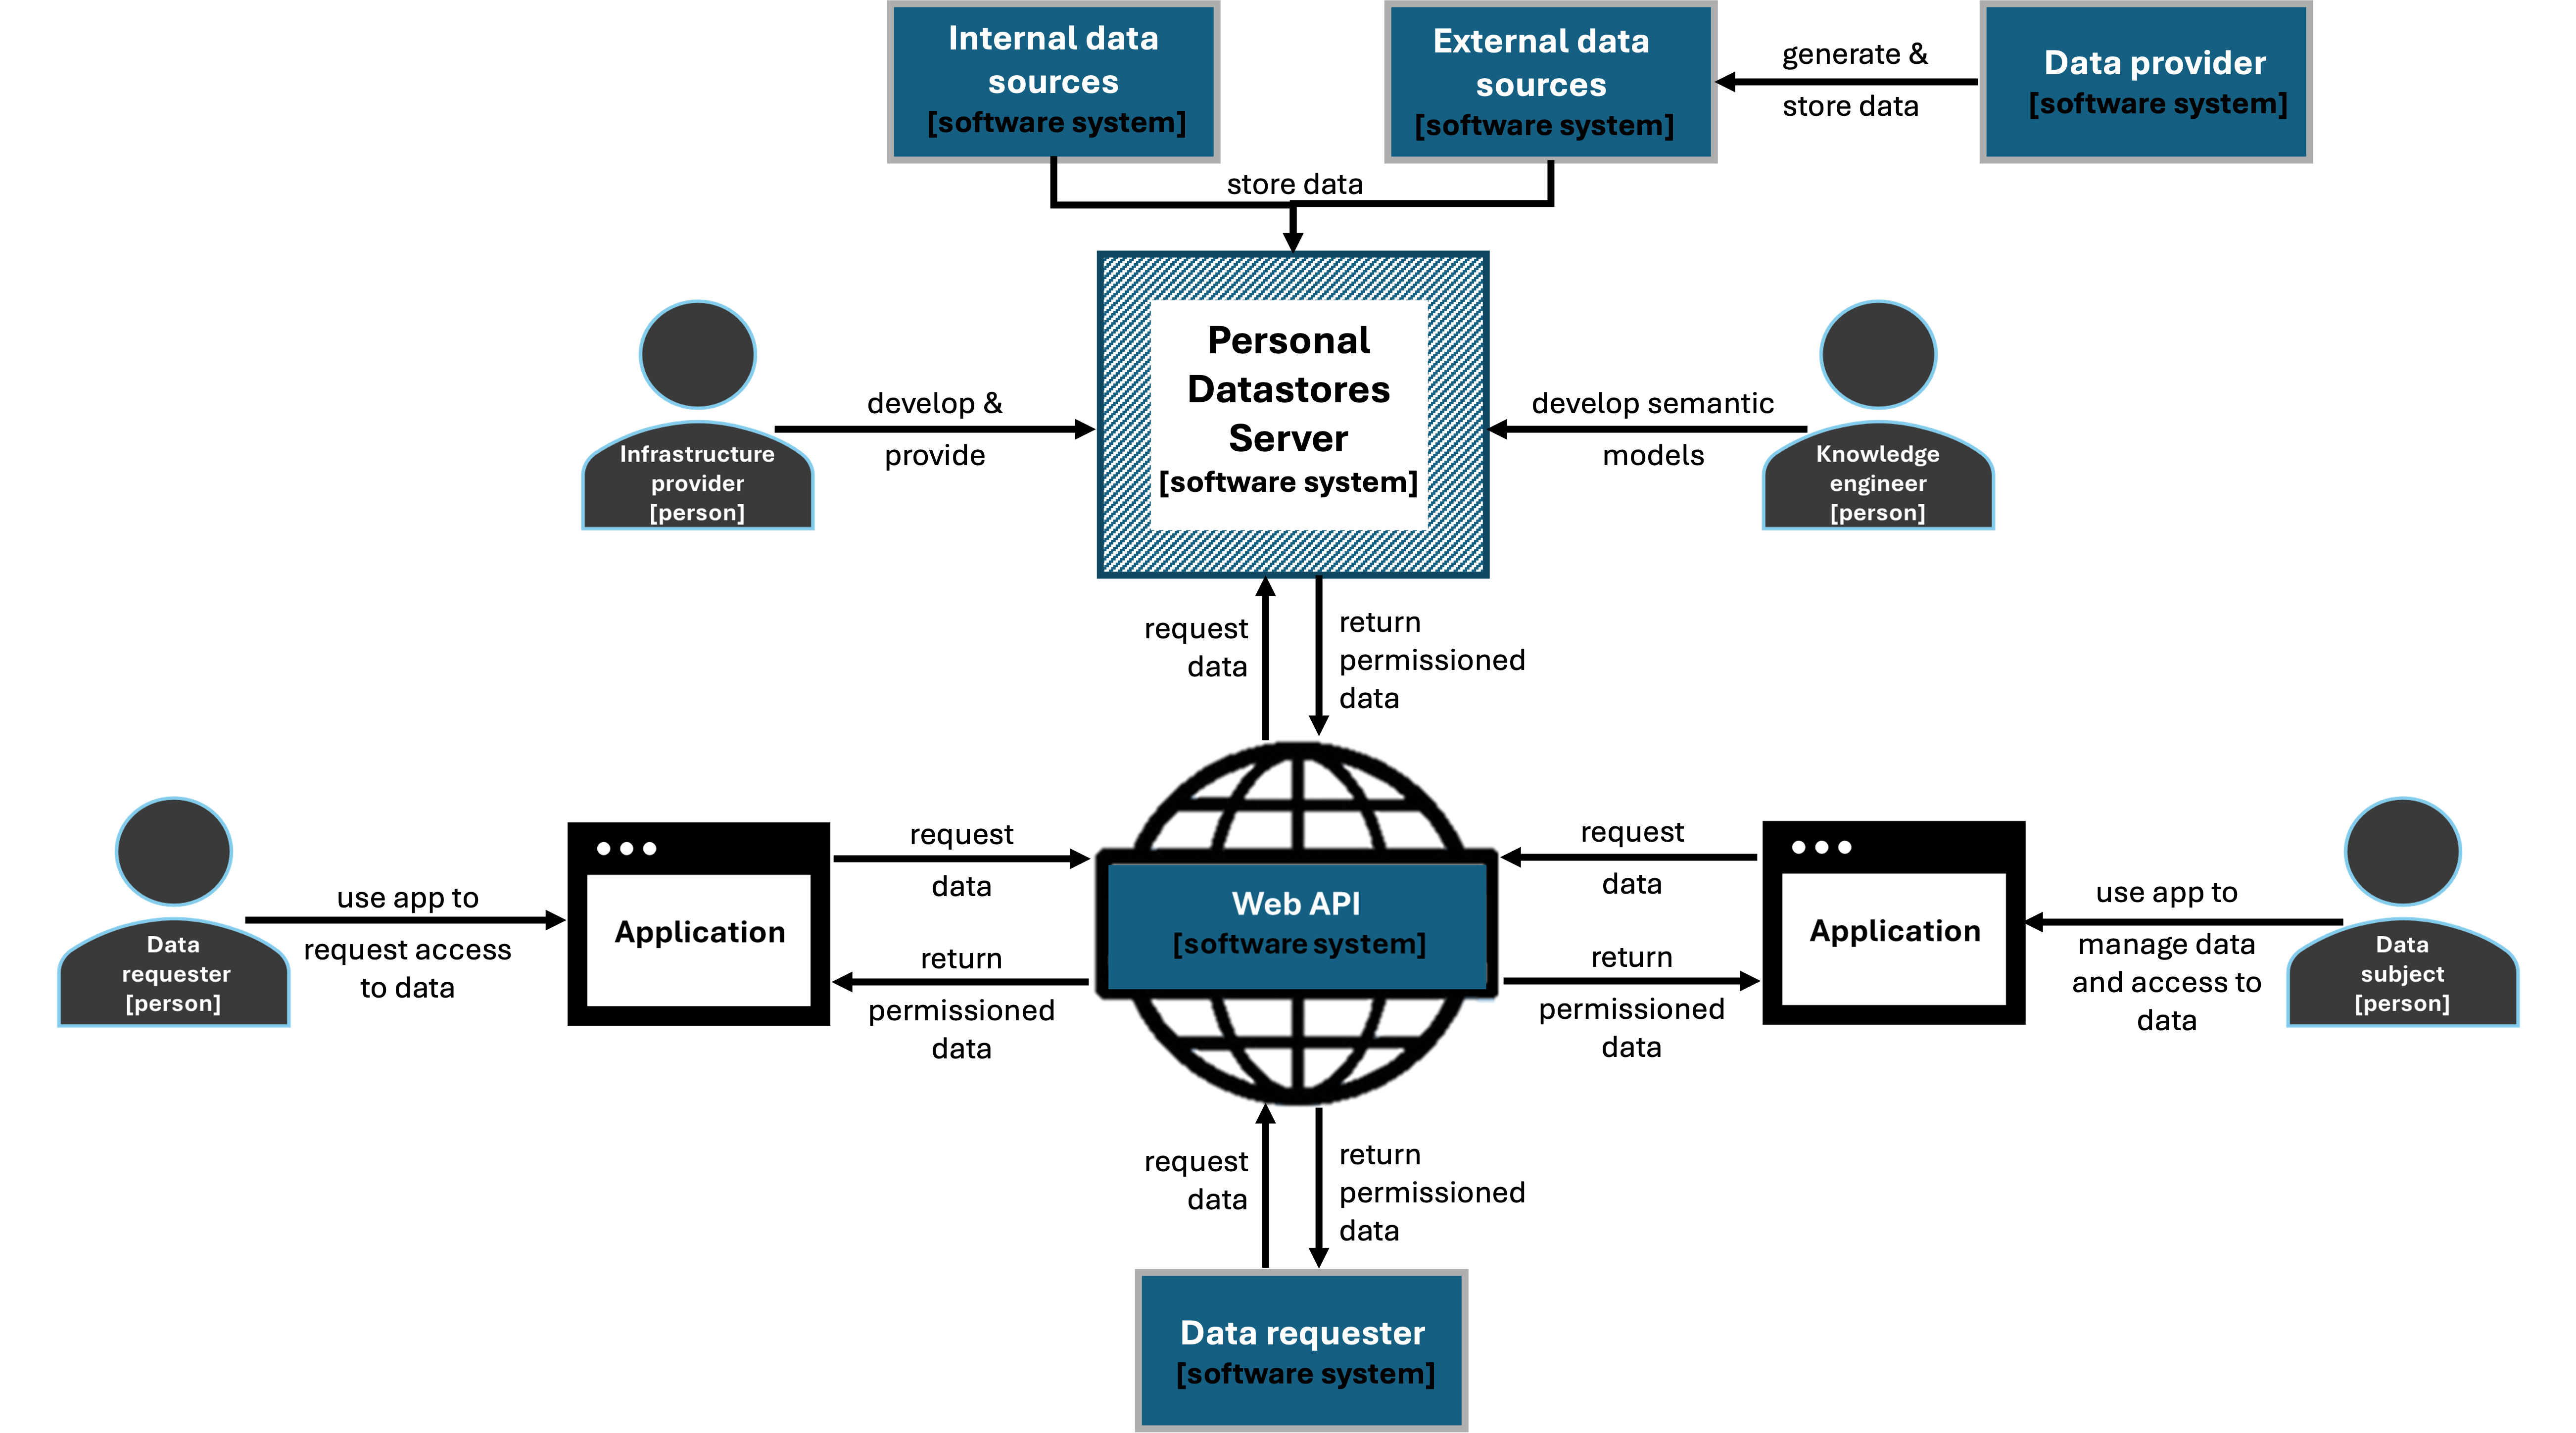
\includegraphics[width=1\linewidth]{figures//chapter-6/system-context-diagram.png}
    \caption{System context diagram of a decentralised data sharing ecosystem.}
    \label{fig:c4-context}
\end{figure}

In this diagram, the \textit{Infrastructure provider} and the \textit{Knowledge engineer} develop and provide services and semantic models for the main software system described in this Section, the \textit{Personal Datastores Server}.
Datastores hosted in this server are populated by internal and external data sources, such as temporal and spatial data sources, respectively.
The server also provides the access control layer of the ecosystem, allowing data requests and the return of permissioned data to be consumed by Web APIs.
Such APIs can be used by \textit{Data requesters} to consume and generate data, and also to feed Web applications that are used by individuals to request and use data.
Moreover, data subjects can also use applications to manage their data and who/what can have access to it under which conditions.

The \textit{Personal Datastores Server} depicted in this Figure will be further decomposed into containers in the next Section.

\subsection{Container modelling of a decentralised personal datastore server}
\label{sec:c4_container}

The \textit{Container} diagram in Figure~\ref{fig:c4-container} illustrates current and proposed containers within a decentralised personal datastores server.
In a completely decentralised scenario, each container could be developed and/or provided by a distinct \textit{Infrastructure provider}.
The \textit{Notifications}, \textit{Authentication} and \textit{Authorisation} containers are already part of the Solid protocol specification \citep{capadisli_solid_2022} and are not further updated in this Thesis.
To ensure compatibility with the current access control mechanisms, the \textit{Offer Instantiation} and \textit{Agreement Generator} containers are treated separately from the \textit{Authorisation} container.
In this way, systems that currently rely on WAC or ACP to provide access to data can continue to work efficiently, while use cases that involve personal data can use OAC policies to have data-sharing agreements aligned with European data protection law.
ACL and ACP authorisations can be generated, when an agreement for data access has already been reached, for automated access to data when a legally-aligned agreement for access is already in place.
The \textit{Notifications} container can also be updated to support the new access control system proposed in this Thesis, however, this is out of the scope of this contribution.

\begin{figure}[ht]
    \centering
    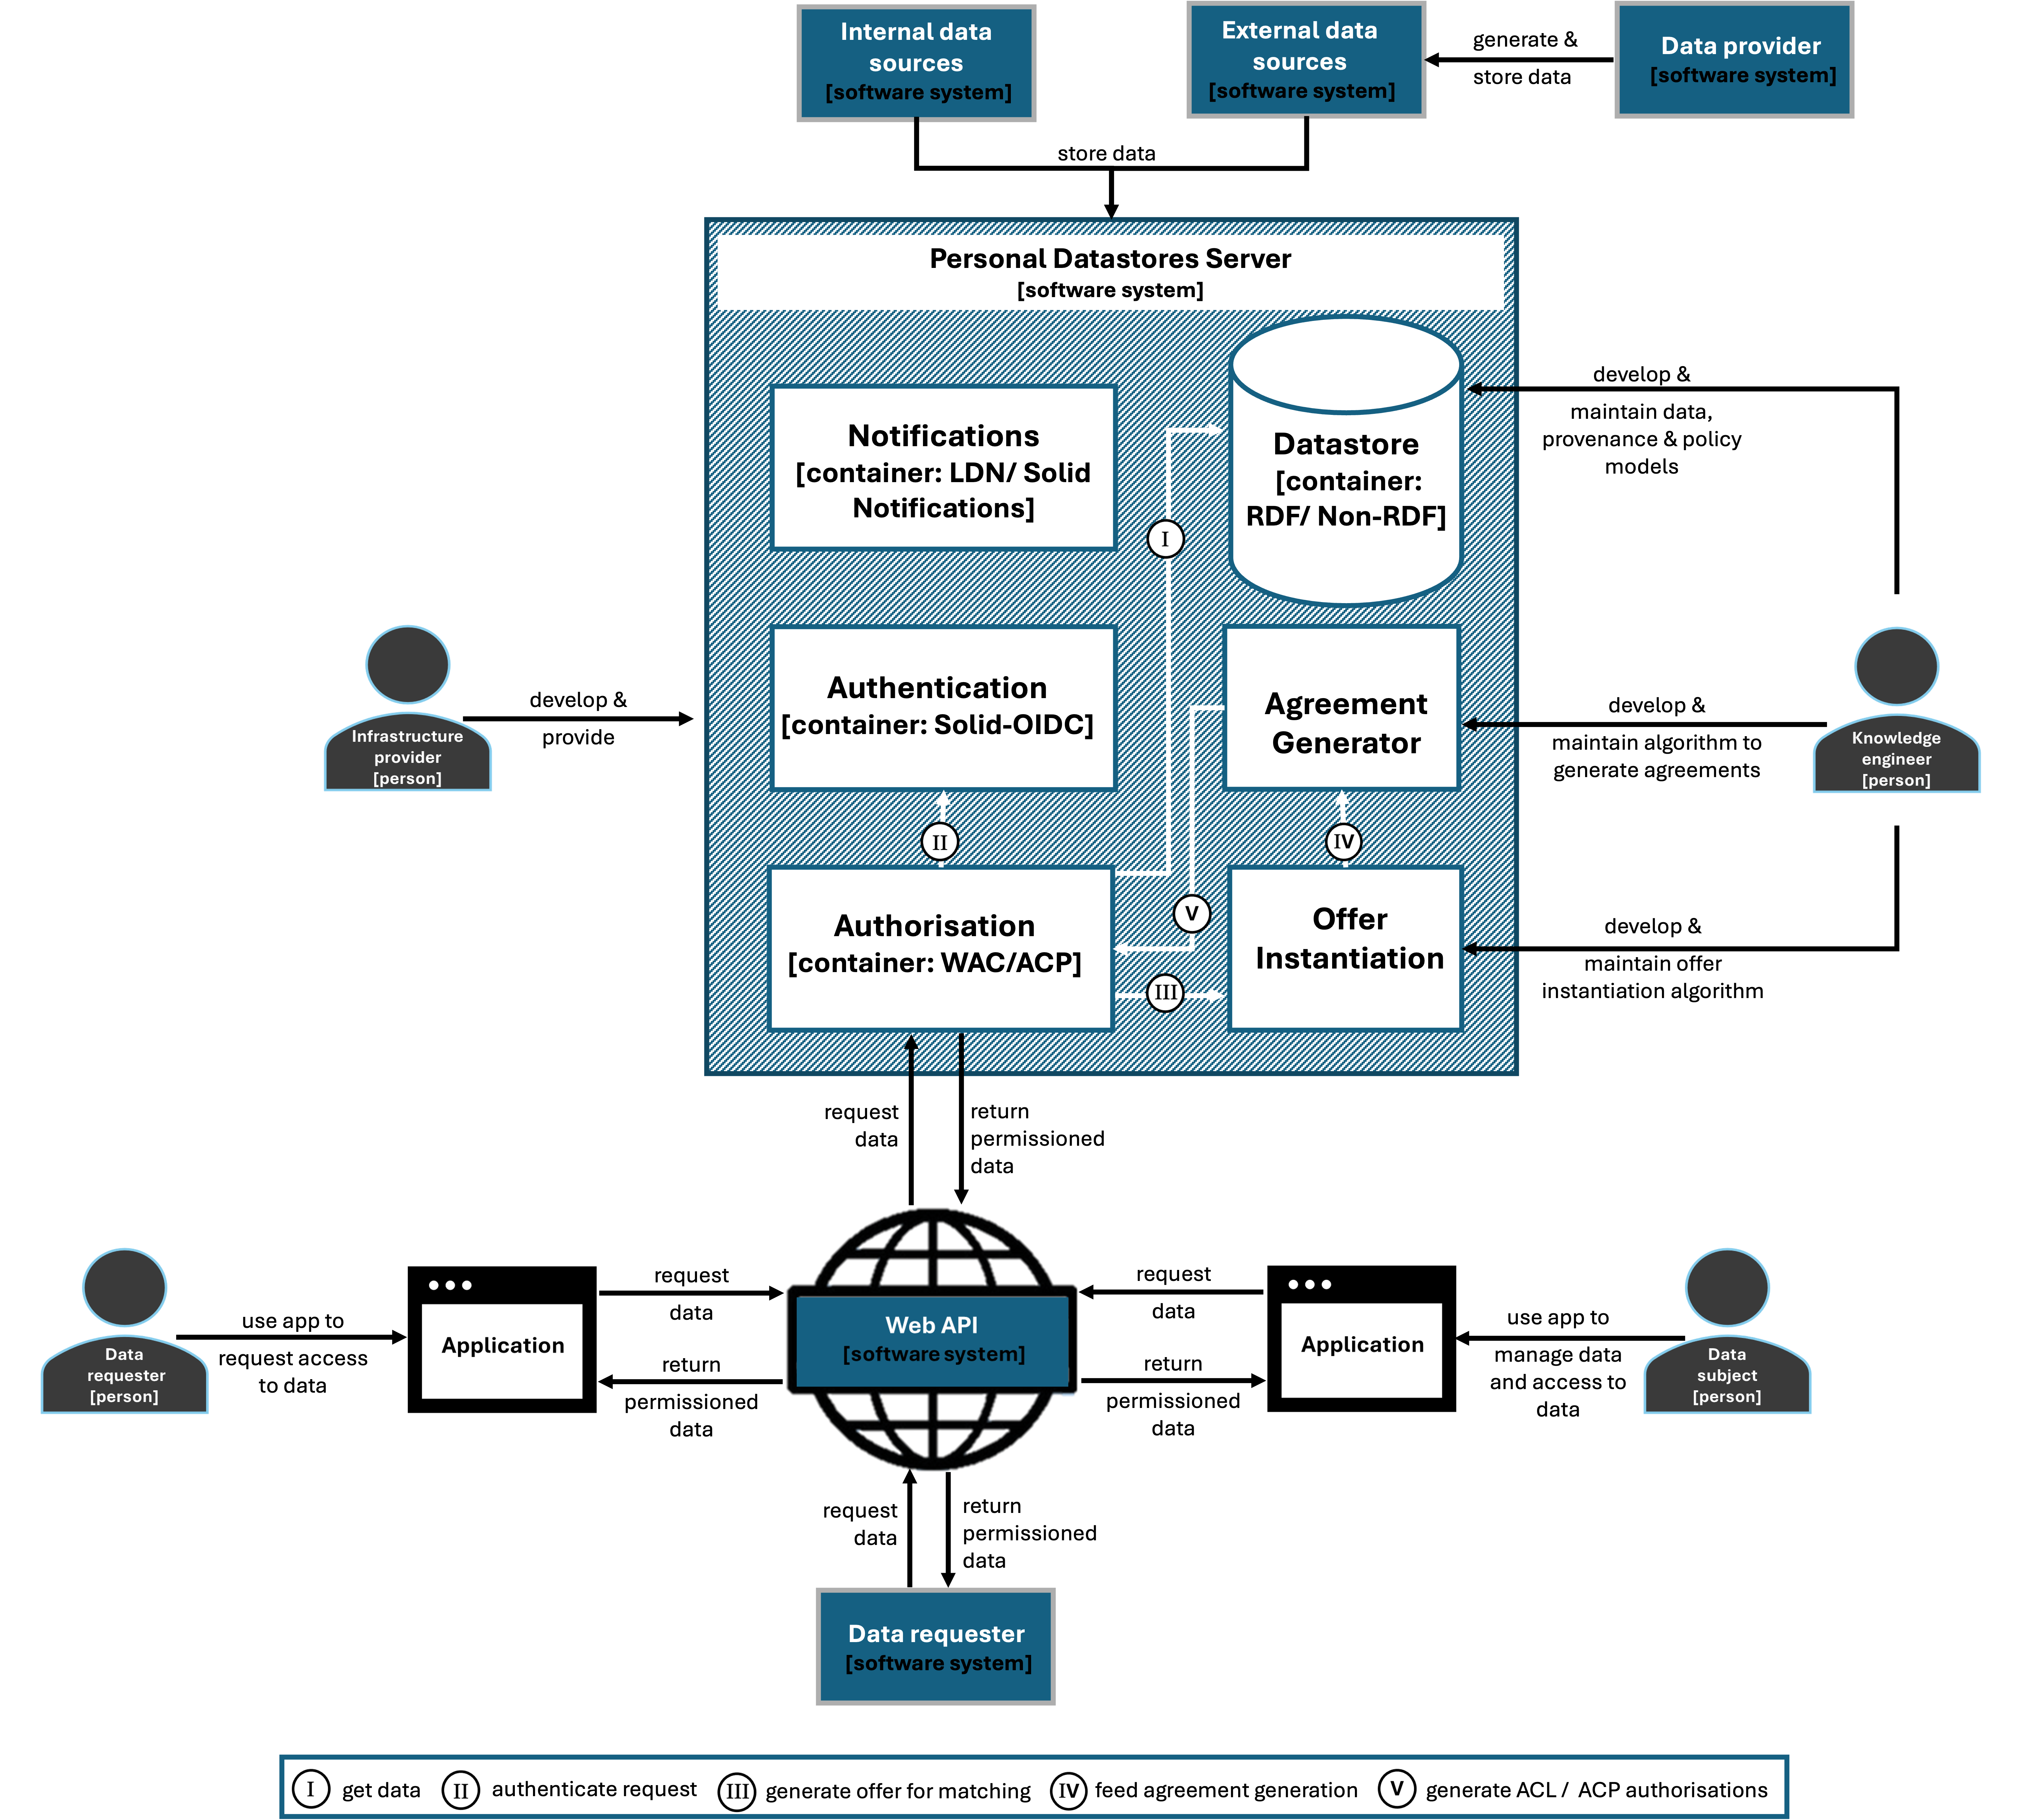
\includegraphics[width=1\linewidth]{figures//chapter-6/container.png}
    \caption{Container diagram of a decentralised personal datastore server.}
    \label{fig:c4-container}
\end{figure}

Furthermore, while an intricate part of the Solid protocol already, the \textit{Datastore} container is further expanded in this Thesis with additional components related to policies and provenance metadata.
The vocabularies developed in Chapter~\ref{chap:vocabularies} should be further developed and maintained by a \textit{Knowledge engineer} and are used to specify data, provenance, and policies, as well as to feed the \textit{Offer Instantiation} and \textit{Agreement Generator} containers.
The \textit{Offer Instantiation} container gathers and instantiates ODRL offers, such as the one in Listing~\ref{list:oac_offer}, which are fed to the \textit{Agreement Generator} container.
This instantiation process takes the user's preferences and requirements to create a context-appropriate offer policy, i.e., directly applicable to the data request.
While the instantiation of offers for specific data requests is not conducted in this Thesis, in Section~\ref{sec:poc_health}, there is a description and implementation of the construction of odrl:Offer instances for a particular use case related to health data-sharing.
The \textit{Agreement Generator} depicted in Figure~\ref{fig:c4-container} will be further decomposed into components in the next Section.

\subsection{Component modelling of a datastore and an agreement generator}
\label{sec:c4_component}

The \textit{Component} diagram in Figure~\ref{fig:c4-component} further decomposes the \textit{Datastore} and \textit{Agreement Generator} containers within a decentralised personal datastores server.
As previously discussed in Sections~\ref{sec:oac} and~\ref{sec:plasma}, for a legally-aligned decentralised ecosystem where personal data is exchanged according to the requirements of the GDPR, information regarding the entities (e.g., providers, developers), infrastructure, legal roles, policies, notices, registries, and logs is necessary to understand and establish responsibilities and accountability within the whole ecosystem.
As such, beyond keeping \textit{Data} in distinct formats, \textit{Datastores} are expected to keep (i) \textit{Policies}, including user requirements and preferences, copies of data requests and records of data access agreements, (ii) \textit{Notices}, e.g., to declare the providers/developers of apps, service, or other infrastructures, as well as to describe their data processing practices, (iii) \textit{Logs}, related to actions on data, policies, or security issues, which can be used by external auditors to perform their duties, (iv) \textit{Registries}, for collective and convenient access to data, and (iv) other \textit{Provenance} metadata, all needed to have a trustful and sustainable decentralised data sharing ecosystem.
As such, the semantic models produced in Chapter~\ref{chap:vocabularies} play an important role in having interoperable datastores where data can be consumed by multiple parties in a lawful manner, even if said parties resort to the use of different providers.

\begin{figure}[t]
    \centering
    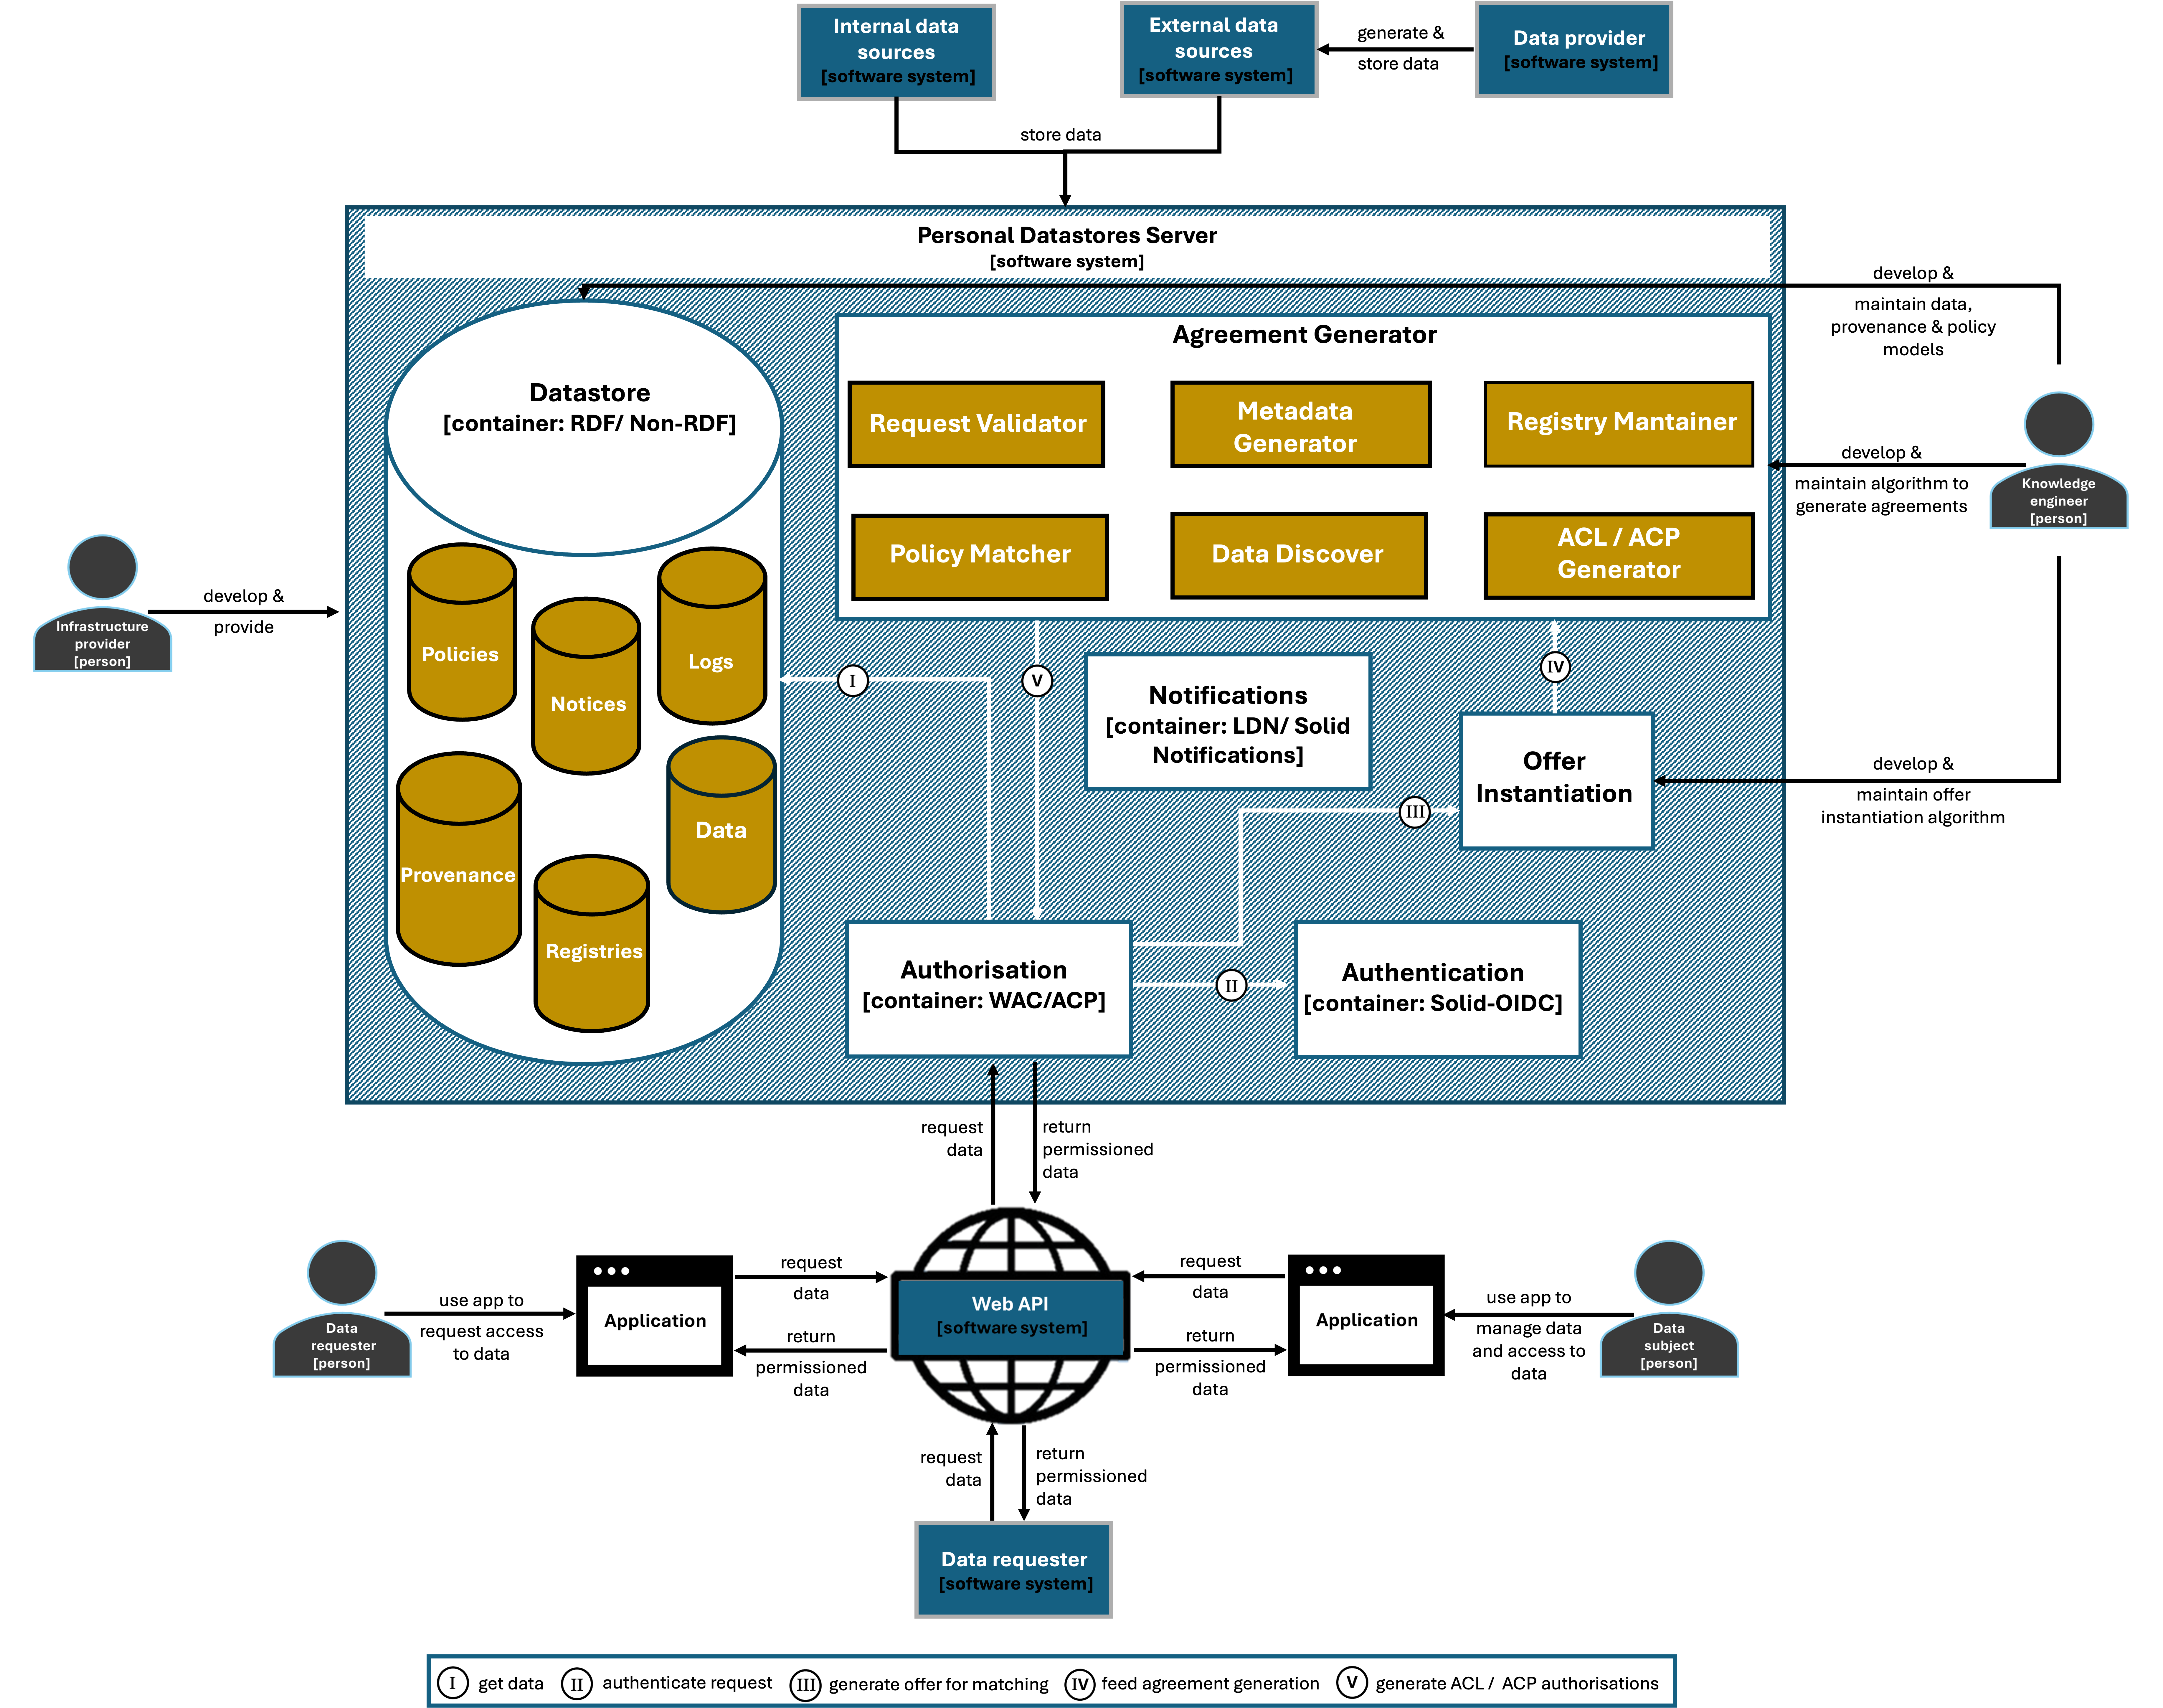
\includegraphics[width=1.1\linewidth]{figures//chapter-6/component.png}
    \caption{Component diagram of a datastore and an agreement generator.}
    \label{fig:c4-component}
\end{figure}

When it comes to the architecture of the \textit{Agreement Generator}, the following components were identified:

% TODO: https://github.com/RDFLib/pySHACL
\begin{itemize}
    \item The \textit{Request Validator} component has the main goal of validating RDF-based data requests against the conformance conditions established in Section~\ref{sec:plasma_conformance}, using technologies such as SHACL~\citep{knublauch_shapes_2017} or ShEx~\citep{prudhommeaux_shape_2019}. This component is of fundamental importance to ensure that all legally required data is present in the data request and to guarantee that the data request can be fed to the policy matcher in the expected format.
    \item The \textit{Metadata Generator} and \textit{Registry Maintainer} components have the main goal of generating and storing logs and other metadata related to entities, apps, services, or Pods and maintaining updated registries of access control authorisations, availability of data categories, supported schemas for data, and relevant policies, apps, services, users, or agents.
    \item The \textit{Data Discover} component's main task is to provide the server with data discovery capabilities in order to more easily find where certain types of data, policies, or provenance metadata are stored, including storage locations outside the server.
    \item The \textit{Policy Matcher} component, further specified in Section~\ref{sec:algorithm}, has the main goal of matching the existing user offers with incoming data requests and generate data-sharing agreements. These agreements are then fed to the \textit{ACL/ACP Generator} component for seamless integration into the current Solid ecosystem.
\end{itemize}

Indeed, to understand the detailed functionality of the proposed personal datastores server, Figure~\ref{fig:c4-sequence} presents a sequence diagram to demonstrate how its containers, and more specifically its components, interact with each other when a data requester uses an app to petition a certain type of data to be used for a particular purpose.

\begin{landscape}
\begin{figure}[htp]
    \centering
    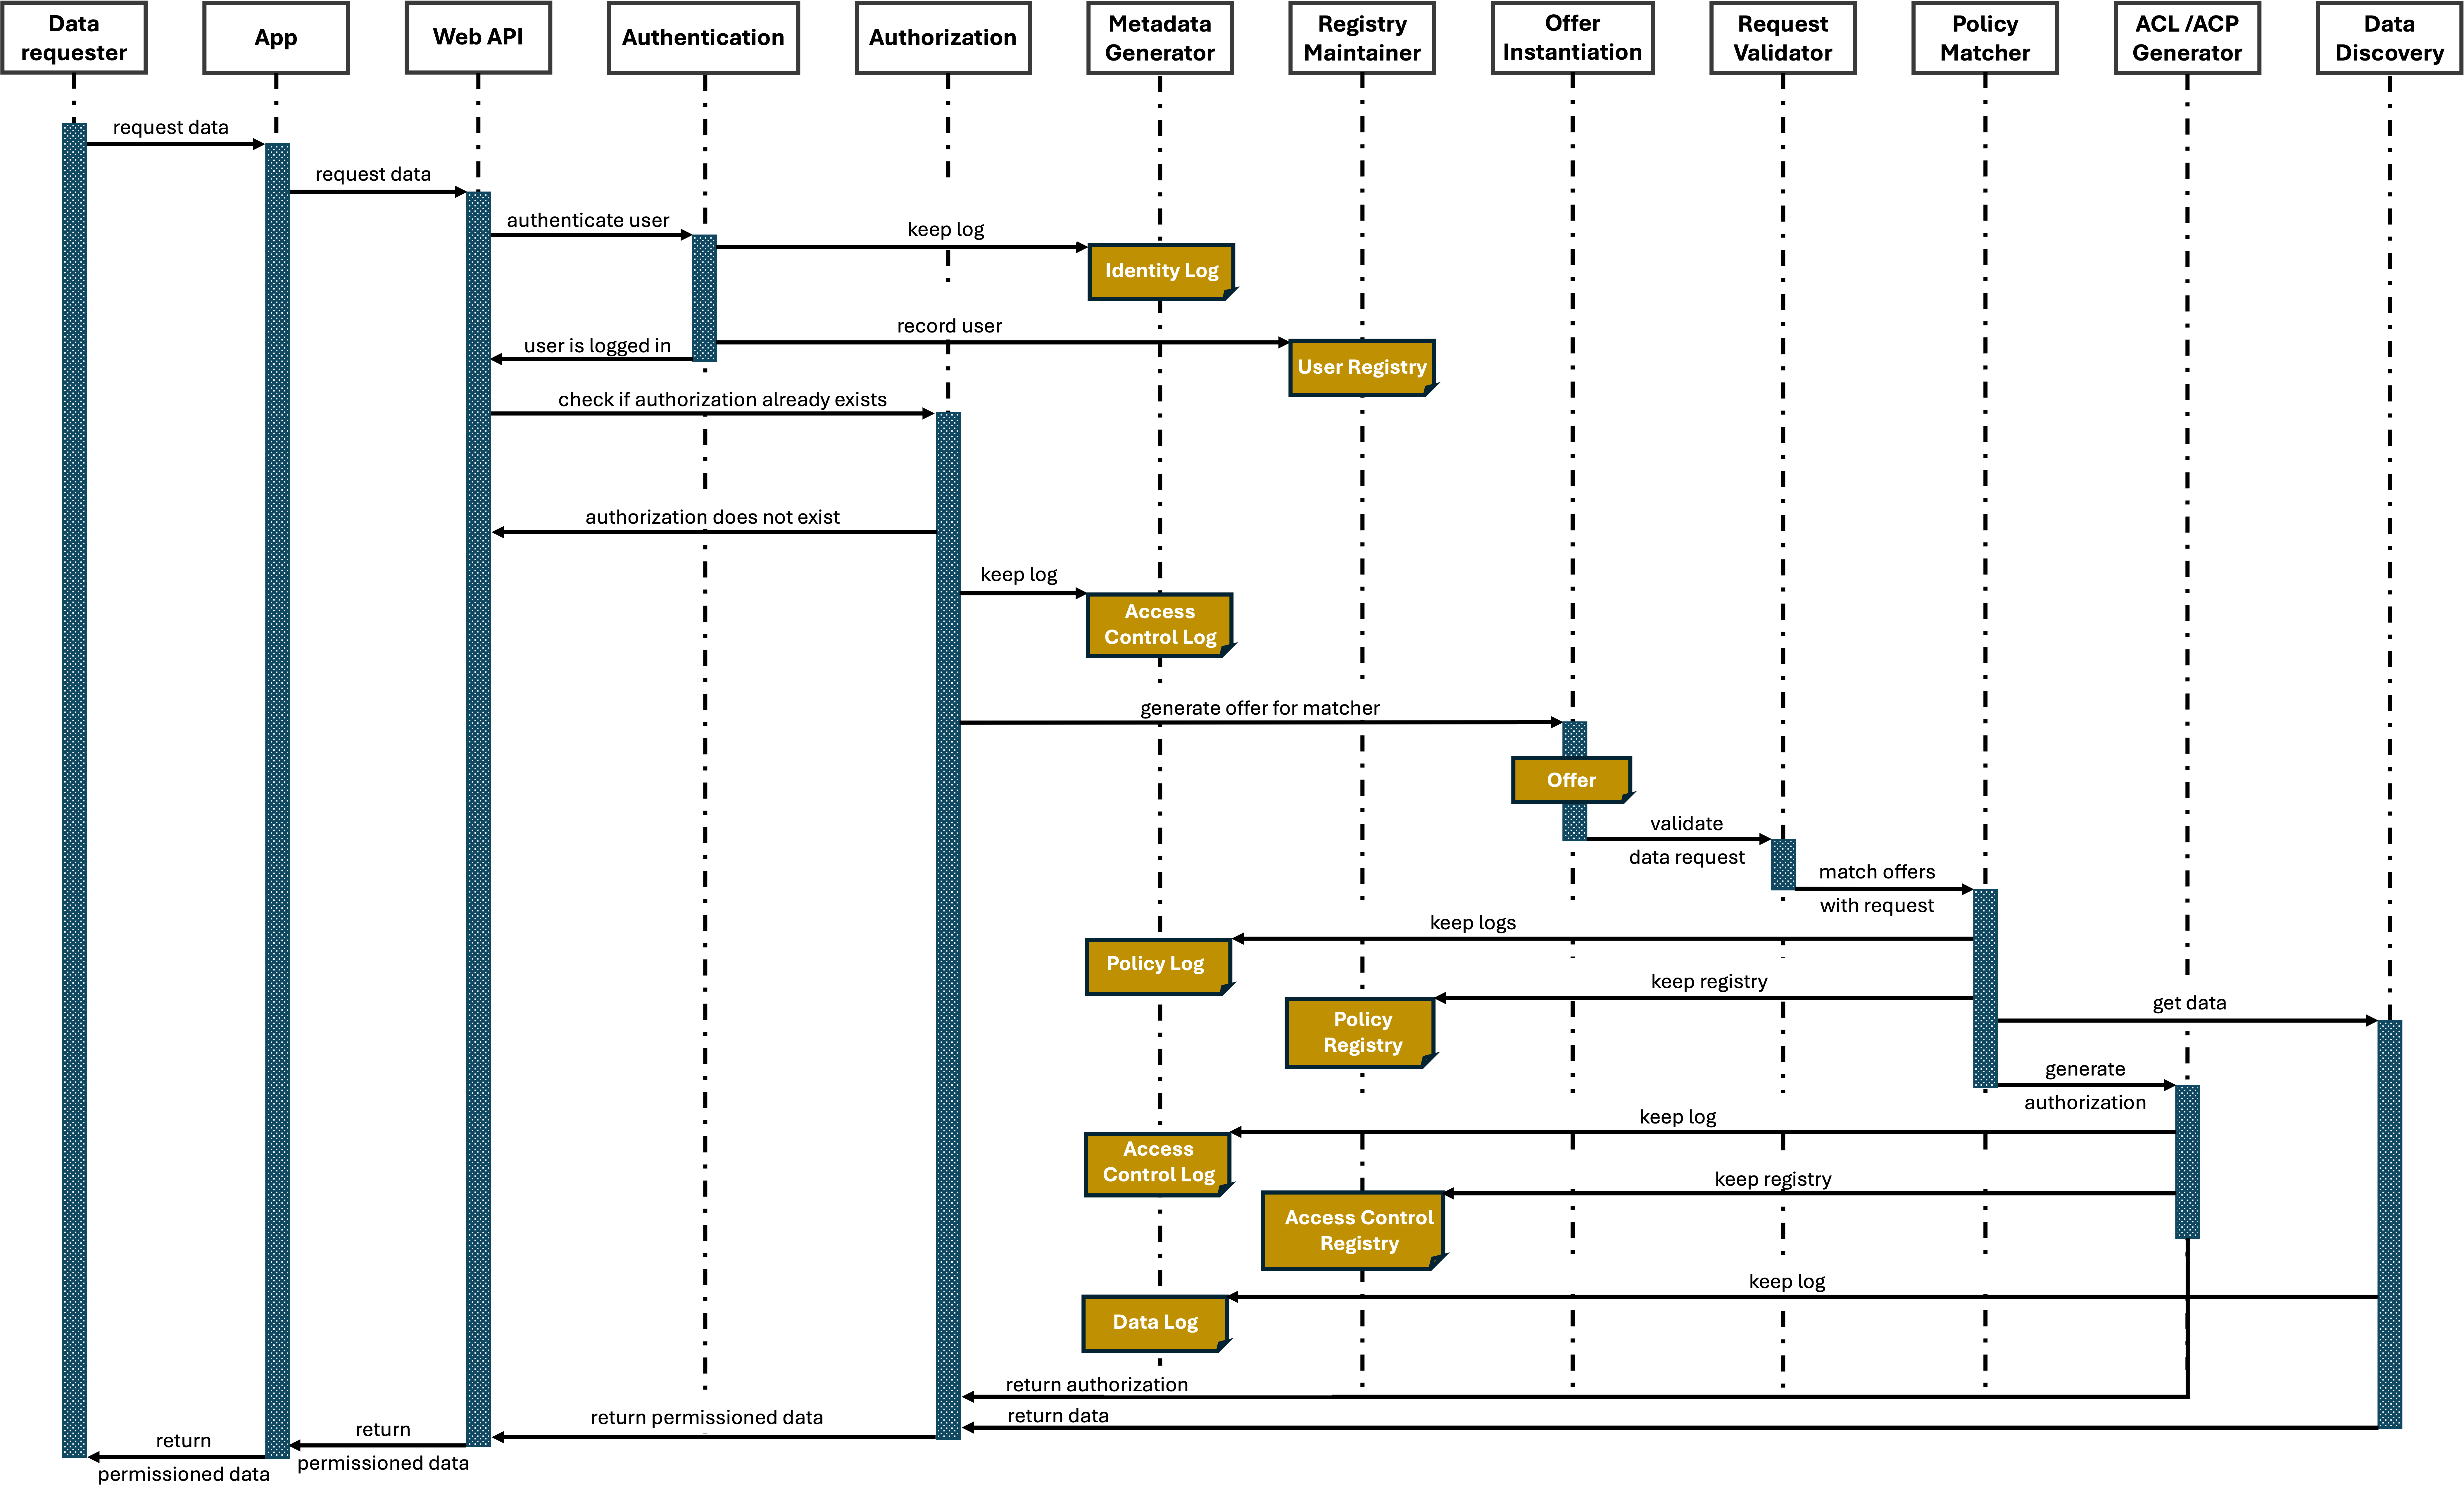
\includegraphics[width=1\linewidth]{figures//chapter-6/sequence.png}
    \caption{Sequence diagram of data access request using proposed architecture.}
    \label{fig:c4-sequence}
\end{figure}
\end{landscape}

When data requesters want to have access to a certain resource or data type, they can either use an app to do it, as in Figure~\ref{fig:c4-sequence}, or directly do a request through the Web API.
When using an app, the request is then transmitted to the Web API and in turn, the requester must be authenticated to get access to non-public data.
After the authentication process goes through, or also in the cases where requesters cannot successfully log in, an identity log is recorded.
Additionally, information about the data requester is also recorded in the user registry of the data subject.
If a previously-given authorisation is still valid, then access to data can be given, however, in Figure~\ref{fig:c4-sequence}, this authorisation does not exist, a fact which could also be kept in an access control log.

Therefore, as there are no ACL nor ACP authorisations in place, an offer with the data subject's policies should be instantiated in order to feed the agreement generator.
This instantiation is followed by the validation of the data request, to ensure that it is in the correct format, and both are fed to the policy matcher component for the generation of a data access agreement.
A log of the policy matching and its result should be kept and the resulting agreement should be added to the policy registry.
In case the result is negative, access to data is prohibited, contrarily to the scenario depicted in Figure~\ref{fig:c4-sequence}.
On the other hand, if the result is positive, access to data is permitted, under certain conditions, and an ACL and/or ACP authorisation is generated.
Afterwards, an access control log is recorded and the new authorisation is kept in the access control log for future usage.
Finally, the data discover mechanism is used to find the data being requested and this data is returned to the Web API and next to the app for the data requester to have access to it.

In the next Section, the algorithms for offer instantiation and for policy matching are further explored, with the goal of generating data-sharing agreements that are aligned with legal requirements.
\section{Design of a policy matching algorithm for generating data access agreements}
\label{sec:algorithm}

In this Section, a detailed overview is given of the proposed algorithms for offer instantiation and policy matching towards the generation of a common data access agreement.
Moreover, a policy editor to define and store OAC policies in Solid Pods is described, as well as a REST API service that uses the results of the policy matching algorithm to facilitate the exercising of data subject rights.

\subsection{Development of an OAC policy editor}
\label{sec:sope}

This Section features an ODRL editor designed to define and save RDF policies, to enable the granting of access to personal data stored in Solid Pods.
RDF policies are articulated using the OAC specification developed in Section~\ref{sec:oac}.
As such, with such an OAC editor, data subjects can create intricate, detailed policies that adhere to GDPR stipulations concerning personal data processing without the burden of knowing ODRL or even RDF.

\paragraph{SOPE -- the Solid ODRL access control Policies Editor}
SOPE is a Solid-based app for data subjects to define and store ODRL policies, based on the OAC specification, on Solid Pods.
Detailed instructions on how to install, launch, and use the app are available on the source code repository\footnote{\url{https://w3id.org/people/besteves/sope/repo}}.
To use it, data subjects must already be in the possession of a Solid Pod and a WebID to be able to log into their Pod and store policies there, using SOPE.
Once logged in, users can select the type of policy they want to model, as well as choose the types of personal data and purposes to which the policy applies.
Additionally, users can also select what type of access they which to provide for said data type and purpose, as well as model further constraints, such as types of recipients that can receive the results of the personal data processing or identity providers used by data requesters to authenticate.
Finally, the prototype interface allows users to generate and store the ODRL policy's RDF in the Pod, without the need for users to be knowledgeable about OAC, ODRL, or DPV.
SOPE also stores policy logs and updates the policy registry in the user's Pod, using the PLASMA vocabulary to model such information, however, in the future, such documentation should be generated by the server to ensure interoperability (by not depending on the app's own implementation, which could diverge from app to app).
All generated information, e.g., policies, logs, and registry, is stored in a private location within the Pod -- only authorised users, apps, or services will have access to it if desired by the data subject.
Figure~\ref{fig:sope-ui} presents a screenshot of SOPE's interface.

\begin{figure}[ht]
    \centering
    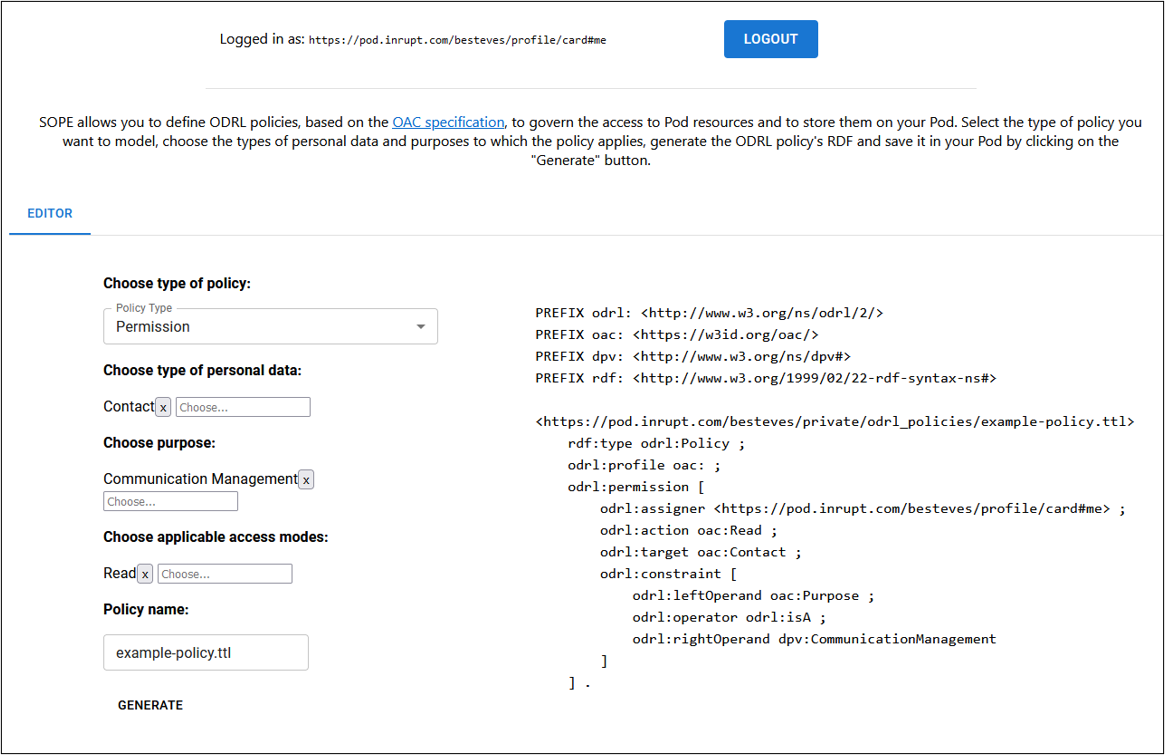
\includegraphics[width=0.9\linewidth]{figures//chapter-6/sope-snap.png}
    \caption{Screenshot of SOPE, a Solid app for editing OAC-based policies.}
    \label{fig:sope-ui}
\end{figure}

\paragraph{SOPE coverage, maintenance, and future work}
SOPE is published and archived according to the methodology described in Section~\ref{sec:code_preservation}.
Furthermore, SOPE's source code is hosted at \url{https://w3id.org/people/besteves/sope/repo}, under the CC-BY-4.0 license.
A live demonstration of the app's features is also available at \url{https://w3id.org/people/besteves/demo/eswc22}.
The repository can also be used by SOPE users to suggest new features to be added to the app and to report bugs through GitHub Issues.
%\beatriz{Table XX } illustrates the current coverage of SOPE concerning the terms implemented in the app from DPV's taxonomies of purposes, personal data categories, processing operations, and recipients.
Currently, SOPE's app coverage encloses terms from DPV's taxonomies of purposes, personal data categories, processing operations, and recipients.
As future work, SOPE can be extended to include all terms present in the previously mentioned DPV's taxonomies, as well as to cover all constraints defined in the OAC profile, e.g., restrict legal bases or specify the technical and organisational measures used by data controllers to ensure the secure processing of personal data.
Moreover, with such an extension, SOPE could also be used by data controllers to detail their privacy policies.
Additionally, user studies should be performed to assess the design choices included in the editor, as well as to understand what type of additional controls people want to have on top of what is legally mandated, e.g., temporal constraints or duties for the data controller to fulfil prior to data access.

\subsection{Data subject policies as \texttt{odrl:Offer}s}
\label{sec:algorithm-offer}

Data subjects can express policies for specific resources, containers of resources, specific personal data types, or even for data they have not produced yet.
As such, at the time of instantiation, the incoming data request should be used to filter the data subject's policies that apply to that particular request.
This is to ensure that only the needed policies are shared and no more, aligned with the `data minimisation' principle in GDPR's Article 5.1(c) \citeyearpar{noauthor_regulation_2016}, as user policies should also be considered personal data and be treated as such.
Therefore, the resulting \texttt{odrl:Offer} instance contains the union of all pertinent user policies, which can be used to match against incoming data requests in order to generate data access agreements for certain resources or data.
Furthermore, this policy can be used as metadata that accompanies the data being accessed/shared, so that data controllers can keep a copy of the conditions under which they can use the data.
In essence, such a system improves trust and accountability in decentralised data-sharing ecosystems as the policy can travel with the data, with provenance information on who generated the data, who generated the policy, and who attached it to the data.
Even though malicious agents can perform prohibited actions, such as making copies of data when only read-access to data was allowed, with the documentation of access conditions being stored on the datastore of the data subjects, they can use these policies and metadata to file a complaint in the court of law for data misuse.
Moreover, when formulating offers, each distinct rule merged into the policy is preserved as an individual rule to facilitate the matching with data requests.
This preservation of individual rules also enables their individual annotation with provenance metadata, e.g., their origin or whether they are negotiable or non-negotiable rules.

Taking this into consideration, the instantiation of the \texttt{odrl:Offer} should follow the subsequent algorithm:
\begin{enumerate}
    \item For a given personal datastore, retrieve all user preferences and requirements recorded in a datastore policy registry.
    \item Filter out duplicated policies.
    \item Filter out policies that do not match with any terms of the data request.
    \item For each retrieved policy, fetch relevant \texttt{odrl:Permission} and \texttt{odrl:Prohibition} rules and merge them in a single \texttt{odrl:Offer}.
    \item Permissions and/or prohibitions associated with an OAC requirement or an OAC preference should be associated with the term \texttt{dpv:Required}, in case said rule is a requirement, or the term \texttt{dpv:Optional}, in case it is a preference, using the \texttt{dpv:hasContext} property.
    \item A link to each `original' policy is maintained in the final \texttt{odrl:Offer} by using the \texttt{dcterms:source} property.
    \item Add provenance information to the \texttt{odrl:Offer}, e.g. \texttt{dcterms:issued} for when the offer was instantiated and \texttt{dcterms:creator} for the issuer of the policy.
\end{enumerate}

The previously described Listing~\ref{list:oac_offer} presents an example of a result of the offer instantiation algorithm, generated from two existing, relevant policies, as indicated by the \texttt{dcterms:source} property, based on an OAC requirement and OAC preference policies, as expressed by the \texttt{dpv:hasContext} property.

\subsection{Policy matching outcomes as \texttt{odrl:Agreement}s}
\label{sec:algorithm-agreement}

As mentioned in the previous Sections, the instantiated user policies are one of the few bits, representing the will of the data subject, that must be fed to the policy matching algorithm to generate the data access conditions to certain data or resources.
In addition to those, data request policies, expressing the needs and purposes of the data requesters, as well as other contextual information, e.g., date or time of the day, must also be passed on to the algorithm in order to reach a data access agreement that benefits and satisfies both parties.

The recorded outcomes, resulting from the matching process where access to data needs to be either permitted or prohibited, are instances of \texttt{odrl:Agreement}.
Within these agreements, specific ODRL terms play a crucial role in specifying who has granted or denied access (\texttt{odrl:assigner}), to whom (\texttt{odrl:assignee}), for what resources (\texttt{odrl:Asset}), and the associated conditions for access (\texttt{odrl:Rule}).
Moreover, the rules referenced within an agreement mirror the specific rules outlined for a dataset, i.e., through an \texttt{odrl:Offer}, and within a request, i.e., through an \texttt{odrl:Request}).
As such, by being derived from these rules, an agreement should explicitly reference them to assist in the explainability of the algorithm, e.g., in case the data subject wants to know why a certain data access-related decision was made.
An example representation of a data access agreement, depicted as an \texttt{odrl:Agreement} between two parties to read the Pod's data subject age data for academic research, is provided in Listing \ref{list:oac_agreement}.

Taking this into consideration, the generation of the \texttt{odrl:Agreement} should follow the subsequent algorithm:
\begin{enumerate}
    \item Retrieve the data requester's \texttt{odrl:Request} and the user policy's \texttt{odrl:Offer}.
    \item Match the \texttt{odrl:Offer} with the \texttt{odrl:Request}.
    \item Record the outcome of the matching algorithm, where the \texttt{odrl:target} property specifies the data to be accessed, and the \texttt{odrl:assignee} and \texttt{odrl:assigner} properties identify the requester and the data subject, respectively.
    \item If the matching result is positive, i.e., the request and the offer are compatible, then access is permitted by employing a permission with constraints on the requested purpose for access, along with any additional constraints such as legal bases, identity providers or recipients. If access is denied, similar information is included in the policy as a prohibition.
    \item Utilise the \texttt{dcterms:references} property to associate the agreement with the \texttt{odrl:Offer} and \texttt{odrl:Request} that were used to generate it.
    \item Include provenance and other relevant information, such as the \texttt{dcterms:issued} property, to document the creation and acceptance of the agreement among the parties.
\end{enumerate}

The matching process described in step 2 of agreement generation algorithm operates by comparing and assessing the compatibility between the conditions described in user policies and in data access requests.
In the ODRL-based system proposed in this Thesis, this process involves comparing the data subjects' \textit{odrl:Offer}, stored in their Pods, with an \textit{odrl:Request} of a data requester, app, service or agent.
As such, when considering two sets of concepts representing an offer and a request, the matching algorithm may employ two distinct and incompatible approaches to determining access to data.
The first approach, the one proposed in this Thesis to cater to the specific requirements of GDPR consent described in Chapter~\ref{chap:legal}, which is also the more commonly used semantically, involves treating classes as sets and determining access based on set membership.
In this approach, if a class $P$ is a superclass of $C$, a request for accessing $P$ would also allow access to $C$ because every member of $C$ is inherently a member of $P$.
However, a request for accessing $C$ would not grant access to $P$ since not all members of $P$ are necessarily members of $C$.
This method has also been previously utilised in matching policies for GDPR compliance by \cite{bonatti_realtime_2020}.

The second approach is based on determining the applicability of a concept according to its specificity.
In this method, when considering a class $P$ and its subclass $C$, a request for accessing $P$ would not extend access to $C$ since $C$ is more specific.
Conversely, a request for accessing $C$ would grant access to $P$ as $C$ is less specific.
Employing subsumption as a criterion, in the first approach, access is granted when the user offer subsumes the data request, whereas, in the second approach, access is granted when the data request subsumes the user offer.
Hence, both mentioned approaches can be adapted in a decentralised data access ecosystem by reversing the direction of the subsumption in the policy matching algorithm.

Another factor to consider for the matching algorithm involves resolving permissions and prohibitions in terms of their evaluation order and potential conflicts.
Policies can be interpreted in various incompatible ways, such as prioritising permissions and granting access upon the first one that is fulfilled -- a permissive model.
Contrarily, prioritising prohibitions and denying access upon the first fulfilled prohibition is considered a prohibitive model.
In cases where both a permission and a prohibition apply to the same data or resource, conflict resolution is based on the prevalence of one over the other.
In decentralised data environments such as Solid, the matching algorithm follows a prohibitive model, where prohibitions outweigh permissions.
This means that if a request either fails to satisfy a permission or satisfies a prohibition, data access is not granted.
As such, compatibility between offers and requests is only achieved when all permissions are satisfied and all prohibitions remain unsatisfied.

In light of these considerations, the policy matching algorithm described in this Thesis involves examining subsumption or satisfiability between instances of \texttt{odrl:Offer} and \texttt{odrl:Request}.
The algorithm essentially verifies whether the conditions outlined in the user offer are met by the data request policy in the case of permissions, or breached in the case of prohibitions.
If any prohibitions are identified, it indicates that certain conditions of the proposed data request are incompatible with the policies set by the user to govern the access to their personal data.
Conversely, if no prohibitions are found and all permissions are met, the conditions are deemed compatible and access to data can be provided.
In this context, Algorithm~\ref{alg:matching} offers pseudo-code outlining the steps of the proposed policy matching process.

\begin{algorithm}
\caption{Pseudo-code of the proposed OAC-based matching algorithm.}
\label{alg:matching}
\begin{algorithmic}
\For{$prohibition \gets odrl{:}Offer$}
    \If{$offer{:}target \cap request{:}target \neq\emptyset$}
        $decision \gets DENY$
    \EndIf
    \If{$odrl{:}assignee \in offer{:}prohibition$}
        \If{$offer{:}assignee \equiv request{:}assignee$}
            $decision \gets DENY$
        \EndIf
    \EndIf
    \If{$odrl{:}action \in offer{:}prohibition$}
        \If{$offer{:}action \cap request{:}action \neq\emptyset$}
            $decision \gets DENY$
        \EndIf
    \EndIf
    \For{$constraint \gets prohibition$}
        \If{$oac{:}Purpose \gets constraint$}
            \If{$offer{:}Purpose \cap request{:}Purpose \neq\emptyset$}
                $decision \gets DENY$
            \EndIf
        \ElsIf{$oac{:}Recipient \gets constraint$}
            \If{$offer{:}Recipient \cap request{:}Recipient \neq\emptyset$}
                $decision \gets DENY$
            \EndIf
        \ElsIf{$oac{:}LegalBasis \gets constraint$}
            \If{$offer{:}LegalBasis \cap request{:}LegalBasis \neq\emptyset$}
                $decision \gets DENY$
            \EndIf
        \ElsIf{$oac{:}TOM \gets constraint$}
            \If{$offer{:}TOM \cap request{:}TOM \neq\emptyset$}
                $decision \gets DENY$
            \EndIf
        \ElsIf{$oac{:}Technology \gets constraint$}
            \If{$offer{:}Technology \cap request{:}Technology \neq\emptyset$}
                $decision \gets DENY$
            \EndIf
        \ElsIf{$oac{:}IdP \gets constraint$}
            \If{$offer{:}IdP \cap request{:}IdP \neq\emptyset$}
                $decision \gets DENY$
            \EndIf
        \EndIf
    \EndFor
\EndFor

\For{$permission \gets odrl{:}Offer$}
    \If{$offer{:}target \cap request{:}target =\emptyset$}
        $decision \gets DENY$
    \EndIf
    \If{$odrl{:}assignee \in offer{:}permission$}
        \If{$offer{:}assignee \not\equiv request{:}assignee$}
            $decision \gets DENY$
        \EndIf
    \EndIf
    \If{$odrl{:}action \in offer{:}permission$}
        \If{$offer{:}action \cap request{:}action =\emptyset$}
            $decision \gets DENY$
        \EndIf
    \EndIf
    \For{$constraint \gets permission$}
        \If{$oac{:}Purpose \gets constraint$}
            \If{$request{:}Purpose \not\subseteq offer{:}Purpose$}
                $decision \gets DENY$
            \EndIf
        \ElsIf{$oac{:}Recipient \gets constraint$}
            \If{$request{:}Recipient \not\subseteq offer{:}Recipient$}
                $decision \gets DENY$
            \EndIf
        \ElsIf{$oac{:}LegalBasis \gets constraint$}
            \If{$request{:}LegalBasis \not\equiv offer{:}LegalBasis$}
                $decision \gets DENY$
            \EndIf
        \ElsIf{$oac{:}TOM \gets constraint$}
            \If{$request{:}TOM \not\subseteq offer{:}TOM$}
                $decision \gets DENY$
            \EndIf
        \ElsIf{$oac{:}Technology \gets constraint$}
            \If{$request{:}Technology \not\subseteq offer{:}Technology$}
                $decision \gets DENY$
            \EndIf
        \ElsIf{$oac{:}IdP \gets constraint$}
            \If{$request{:}IdP \not\subseteq offer{:}IdP$}
                $decision \gets DENY$
            \EndIf
        \EndIf 
    \EndFor 
\EndFor

\If{$ \nexists DENY$}
    $decision \gets GRANT$
\EndIf
\end{algorithmic}
\end{algorithm}

The proposed algorithm mirrors the previously described prohibitive approach to matching, where the prohibitions outlined in the user offer are examined and ensured to be met before any permissions are considered.
The denial of the access request occurs during prohibition checking if any of the following constraints in the user offer are found to be incompatible with the data request:

\begin{enumerate}
    \item offer target has a data type matching ($\cap\neq\emptyset$) the target in the data request;
    \item offer assignee matches\footnote{Representing permissions and prohibitions of intricate legal entities such as subsidiaries or company groups accurately is not feasible using equality ($=$) or subset ($\subseteq$) relations. Hence, in this Thesis, the equivalence relation ($\equiv$) is used to signify that the data requester must adhere to the legal interpretation of equality -- defining this equality is beyond the scope of this Thesis.} ($\equiv$) the assignee of the data request; 
    \item offer action has an access mode matching ($\cap\neq\emptyset$) the action in the data request;
    \item offer has a purpose matching ($\cap\neq\emptyset$) the purpose in the data request;
    \item offer has a recipient matching ($\cap\neq\emptyset$) the recipient in the data request;
    \item offer has a legal basis matching ($\cap\neq\emptyset$) the legal basis in the data request;
    \item offer has a technical and organisational measure matching ($\cap\neq\emptyset$) the technical and organisational measure in the data request;
    \item offer has a technology matching ($\cap\neq\emptyset$) the technology in the data request; and
    \item offer has an identity provider matching ($\cap\neq\emptyset$) the identity provider in the data request.
\end{enumerate}

If no prohibitions are identified, the next step is to verify the permissions.
The access request will be denied during permission checking if any of the following constraints in the offer are incompatible with the data request:

\begin{enumerate}
    \item request target does not have a data type matching ($\cap=\emptyset$) the target in the offer;
    \item offer assignee does not match ($\not\equiv$) the assignee of the data request; 
    \item request action does not have an access mode matching ($\cap=\emptyset$) the action in the offer;
    \item request purpose is not compatible or a subset ($\not\subseteq$) of the offer purpose, e.g., DPV's \texttt{ResearchAndDevelopment} in a data request does not match DPV's \texttt{AcademicResearch} purpose in an offer as \texttt{ResearchAndDevelopment} is a superclass of \texttt{AcademicResearch} and, as such, less specific;
    \item request recipient is not compatible or a subset ($\not\subseteq$) of the offer recipient;
    \item offer legal basis does not match ($\not\equiv$) the legal basis of the data request;
    \item request technical and organisational measure is not compatible or a subset ($\not\subseteq$) of the offer technical and organisational measure;
    \item request technology is not compatible or a subset ($\not\subseteq$) of the offer technology; and
    \item request identity provider is not compatible or a subset ($\not\subseteq$) of the offer identity provider.
\end{enumerate}

The described procedures are applied to all permissions and prohibitions outlined in the data subject's offer.
If all permissions and prohibitions are met without any violations, access to the data can be authorised.

Table~\ref{tab:oac-matching-examples} showcases a set of data access agreement's outcomes illustrating the functioning of the matching algorithm concerning permissions and prohibitions, focusing on data type and purpose constraints.
In a semantic-based architectural design, evaluating equivalence ($\equiv$), intersection ($\cap$), and subset ($\subseteq$) necessitates additional considerations beyond the mere interpretation of \texttt{owl:sameAs} or \texttt{rdfs:subClassOf} properties. 
For instance, comparing \textit{Academic Research} as a purpose with a data request for \textit{Research and Development} purpose, using subset ($\subseteq$) for permissions or intersection ($\cap$) for prohibition, mandates both purposes to be articulated in a manner enabling such `hierarchical' or `set-based' interpretations.
In such a case, the matching algorithm entails interpreting \textit{Academic Research} as a \textit{narrower concept} or a \textit{subset} of \textit{Research and Development}, a relationship that can be denoted through various semantic properties, from distinct vocabularies, such as \texttt{rdfs:subClassOf}, \texttt{skos:broader}, \texttt{dcterms:isPartOf}, or even an ad-hoc property such as \texttt{ex:specialisationOf}.
Further complexity emerges when considering the compatibility of purposes, as such relationships cannot be specified in a hierarchical manner.

\begin{table}[ht]
\centering
\caption{Examples of outcomes of the policy matching algorithm.}
\label{tab:oac-matching-examples}
\resizebox{\textwidth}{!}{%
\begin{tabular}{c|c|c||c|c||c|c}
\multicolumn{3}{c||}{\textbf{Offer}} & \multicolumn{2}{c||}{\textbf{Request}} & \multicolumn{2}{c}{\textbf{Outcome}} \\
\hline
Rule & Purpose & Data & Purpose & Data & Decision & Reason \\
\hline\hline
Prohibition & \begin{tabular}[c]{@{}c@{}}Academic\\research\end{tabular} & Contact & \begin{tabular}[c]{@{}c@{}}Research and\\development\end{tabular} & Age & DENY & request purpose $\cap$ offer purpose $\neq\emptyset$ \\
\hline
Prohibition & \begin{tabular}[c]{@{}c@{}}Academic\\research\end{tabular} & \begin{tabular}[c]{@{}c@{}}Age\\range\end{tabular} & Payment & Age & DENY & request data $\cap$ offer data $\neq\emptyset$ \\
\hline
Prohibition & \begin{tabular}[c]{@{}c@{}}Academic\\research\end{tabular} & Contact & Payment & Age & GRANT & \begin{tabular}[c]{@{}c@{}}request purpose $\cap$ offer purpose $=\emptyset$\\request data $\cap$ offer data $=\emptyset$\end{tabular} \\
\hline
Permission & \begin{tabular}[c]{@{}c@{}}Academic\\research\end{tabular} & Age & \begin{tabular}[c]{@{}c@{}}Commercial\\research\end{tabular} & Age & DENY & request purpose $\not\subseteq$ offer purpose \\
\hline
Permission & \begin{tabular}[c]{@{}c@{}}Research and\\development\end{tabular} & Age & \begin{tabular}[c]{@{}c@{}}Academic\\research\end{tabular} & Age range & GRANT & \begin{tabular}[c]{@{}c@{}}request purpose $\subseteq$ offer purpose\\request data $\cap$ offer data $\neq\emptyset$\end{tabular} \\
\end{tabular}}
\end{table}

Hence, any implementation of an OAC-based, policy matching algorithm must be aware of such relationships and carefully consider when is makes sense to employ equivalence, intersection, and subset methodologies using established semantic web interpretations such as the \texttt{rdf:type} and \texttt{rdfs:subClassOf} properties.
As such, to facilitate the consistent application and interpretation of the algorithm, a standardised specification of vocabulary terms is essential.
This specification should clarify how concepts are expressed and how they are to be interpreted within the policy matching process.
For instance, it should specify that any purpose term in an offer or request policy \textit{MUST} be an instance of \texttt{Purpose} and \textit{MUST} be associated with at least one concept in the purpose taxonomy using \texttt{rdf:type} or \texttt{rdfs:subClassOf} properties.
By adhering to such a standardised specification, the matching algorithm can rely on these assertions to accurately interpret the constraints included in both offer and request policies.
To achieve this, in this Thesis, the adoption of DPV's taxonomies is strongly encouraged when defining both offer and request terms to ensure accuracy and explainability of the desired outcomes in the policy matching algorithm.

\subsection{Development of a `Right of Access' API}
\label{sec:right-api}

% This Section features an ODRL editor designed to define and save RDF policies, to enable the granting of access to personal data stored in Solid Pods.
% RDF policies are articulated using the OAC specification developed in Section~\ref{sec:oac}.
% As such, with such an OAC editor, data subjects can create intricate, detailed policies that adhere to GDPR stipulations concerning personal data processing without the burden of knowing ODRL or even RDF.

% \paragraph{SOPE -- the Solid ODRL access control Policies Editor}
% SOPE is a Solid-based app for data subjects to define and store ODRL policies, based on the OAC specification, on Solid Pods.
% Detailed instructions on how to install, launch, and use the app are available on the source code repository\footnote{\url{https://w3id.org/people/besteves/sope/repo}}.
% To use it, data subjects must already be in the possession of a Solid Pod and a WebID to be able to log into their Pod and store policies there, using SOPE.
% Once logged in, users can select the type of policy they want to model, as well as choose the types of personal data and purposes to which the policy applies.
% Additionally, users can also select what type of access they which to provide for said data type and purpose, as well as model further constraints, such as types of recipients that can receive the results of the personal data processing or identity providers used by data requesters to authenticate.
% Finally, the prototype interface allows users to generate and store the ODRL policy's RDF in the Pod, without the need for users to be knowledgeable about OAC, ODRL, or DPV.
% SOPE also stores policy logs and updates the policy registry in the user's Pod, using the PLASMA vocabulary to model such information, however, in the future, such documentation should be generated by the server to ensure interoperability (by not depending on the app's own implementation, which could diverge from app to app).
% All generated information, e.g., policies, logs, and registry, is stored in a private location within the Pod -- only authorised users, apps, or services will have access to it if desired by the data subject.
Figure~\ref{fig:right-app} presents a screenshot of an example Solid-based application that uses the implemented API service.

\begin{figure}[ht]
    \centering
    \fbox{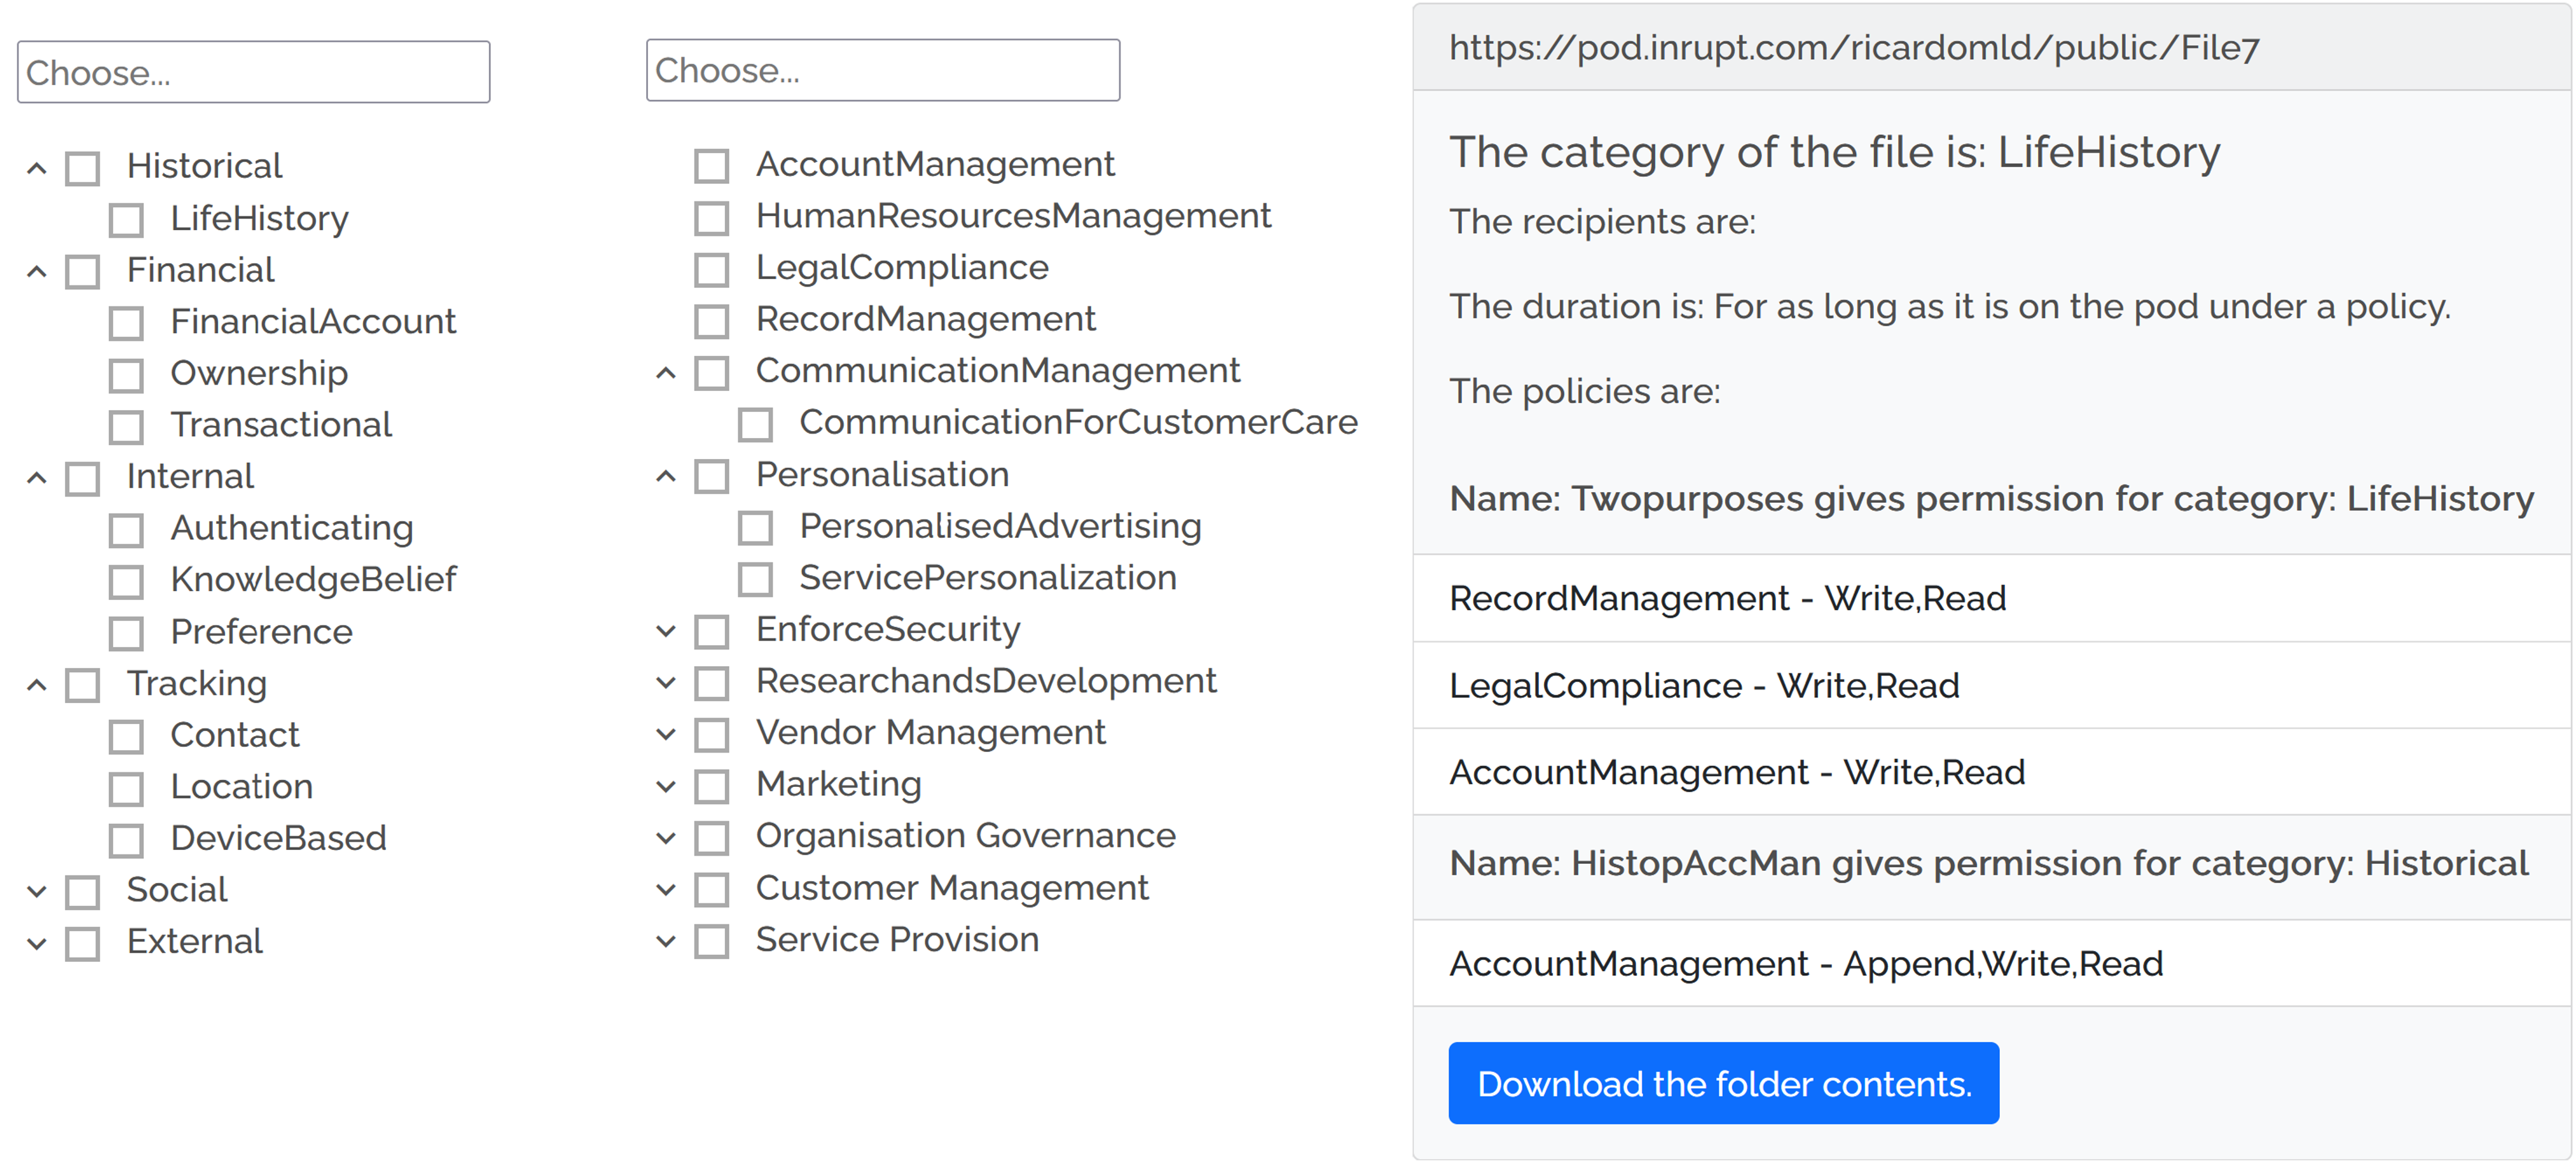
\includegraphics[width=0.8\linewidth]{figures//chapter-6/right-app.png}}
    \caption{Screenshot of an example Solid-based application that uses the implemented Right of Access API.}
    \label{fig:right-app}
\end{figure}

% \paragraph{SOPE coverage, maintenance, and future work}
% SOPE is published and archived according to the methodology described in Section~\ref{sec:code_preservation}.
% Furthermore, SOPE's source code is hosted at \url{https://w3id.org/people/besteves/sope/repo}, under the CC-BY-4.0 license.
% A live demonstration of the app's features is also available at \url{https://w3id.org/people/besteves/demo/eswc22}.
% The repository can also be used by SOPE users to suggest new features to be added to the app and to report bugs through GitHub Issues.
% Currently, SOPE's app coverage encloses terms from DPV's taxonomies of purposes, personal data categories, processing operations, and recipients.
% As future work, SOPE can be extended to include all terms present in the previously mentioned DPV's taxonomies, as well as to cover all constraints defined in the OAC profile, e.g., restrict legal bases or specify the technical and organisational measures used by data controllers to ensure the secure processing of personal data.
% Moreover, with such an extension, SOPE could also be used by data controllers to detail their privacy policies.
% Additionally, user studies should be performed to assess the design choices included in the editor, as well as to understand what type of additional controls people want to have on top of what is legally mandated, e.g., temporal constraints or duties for the data controller to fulfil prior to data access.

\section{Proof of concept implementation for health data sharing}
\label{sec:poc_health}

In this Section, a proof of concept implementation of the proposed algorithms for offer instantiation and policy matching towards the generation of a data access agreement is described for a specific use case involving health data sharing.

\subsection{Background and motivation}
\label{sec:poc_background}

In this Thesis, a health data sharing use case was selected to showcase the strengths of the proposed algorithm since the exchange of health-related data presents significant potential for advancing research and leveraging advanced computational and statistical techniques to drive progress in healthcare.
However, due to its sensitive nature and potentially significant impact if misused, the sharing and utilisation of health-related data are highly regulated at both legal and institutional levels, e.g., \textit{``data concerning health''} is a special category of personal data under the GDPR, i.e., Article 9.1~\citeyearpar{noauthor_regulation_2016}, and as such its processing is prohibited unless one of the legal grounds of Article 9.2 applies.

Currently, institutions such as hospitals handle each health data request through a dedicated committee tasked with evaluating and making decisions regarding the release of such data under their care.
To facilitate this process, the Global Alliance for Genomics and Health\footnote{\url{https://www.ga4gh.org/} (accessed on 2 April 2024)} (GA4GH) was established as an international consortium focused on the development of standards and the promotion of responsible sharing of genomics and health data.
Among its various resources, aimed at different aspects and processes of health-related data sharing, GA4GH has introduced a machine-readable ontology known as the Data Use Ontology\footnote{\url{http://purl.obolibrary.org/obo/duo} (accessed on 2 April 2024)} (DUO).
DUO~\citep{lawson_data_2021,rehm_ga4gh_2021} was designed to express Data Use Limitations (DULs), i.e., conditions and constraints defined by data providers which should be respected by data requesters to use said data.

DUO is an OWL ontology aligned with the Open Biological and Biomedical Ontology\footnote{\url{https://obofoundry.org/} (accessed on 2 April 2024)} (OBO).
By utilising OBO's upper level ontologies, DUO ensures semantic interoperability with a range of biomedical ontologies belonging to the OBO family of ontologies.
As such, DUO's main purpose is related to annotating datasets with DUL codes to specify usage conditions, articulate data usage requests, and automatically identify or discover compatible datasets by comparing requests with datasets' usage conditions.

\paragraph{DUO and existing efforts}
DUO concepts are organised into three taxonomies:
\begin{enumerate}
    \item The `Data Use Permission' taxonomy, denoted by the base class \texttt{obo:DUO\_0000001}, encompasses permissions related to purposes for data usage.
    \item The `Data Use Modifier' taxonomy, denoted by the base class \texttt{obo:DUO\_0000017}, covers additional conditions to be applied alongside data use permissions.
    \item The `Investigation' taxonomy, denoted by the base class \texttt{obo:OBI\_0000066} from the Ontology for Biomedical Investigations\footnote{\url{http://obi-ontology.org/} (accessed on 3 April 2024)} (OBI), delineates planned conditions for which data is being requested.
\end{enumerate}
Furthermore, the \texttt{obo:DUO\_0000010} property implements a \textit{`is restricted to'} relation, used to limit certain concepts to certain contexts, e.g., to restrict the \texttt{obo:DUO\_0000022} concept, which indicates usage permitted within a geographic region, to terms from \texttt{obo:GAZ\_00000448}, the base concept from the Gazetteer (places) ontology\footnote{\url{https://environmentontology.github.io/gaz/} (accessed on 3 April 2024)}.

DUO originated from prior endeavours aimed at establishing consent codes for data usage and leveraging them as machine-readable information for automated access to data.
Its initial development drew upon the Consent Codes by \cite{dyke_consent_2016}, which specified concepts for data usage based on consent permissions.
Subsequently, DUO incorporated a few terms from the Automatable Discovery and Access Matrix (ADA-M) framework \citep{woolley_responsible_2018}, which shares akin objectives and concepts.
As such, the intended utilisation of DUO revolves around facilitating the recording of consent for sharing and reusing biomedical datasets, as outlined by \cite{lawson_data_2021} and \cite{rehm_ga4gh_2021}, the latter highlighting the usage of DUO in distinct GA4GH initiatives.

The Data Use Oversight System\footnote{\url{https://duos.broadinstitute.org/} (accessed on 2 April 2024)} (DUOS) is a platform built upon DUO aimed at facilitating semi-automated management of access health-related datasets.
It leverages DUO annotations to incorporate new datasets and data access requests, which are subsequently matched using an algorithm based on hierarchical compatibility.
Figure~\ref{fig:duo-matching} illustrates the algorithm followed by this platform, where the `Data Use Codes' correspond to concepts from the previously mentioned DUO `Data Use Permission' taxonomy,  the `Data Use Requirements' to the `Data Use Modifier' taxonomy, and the `Research Purpose Terms/Data Use Categories' to the `Investigation' taxonomy.
This algorithm entails matching the dataset's access conditions with the data requester's conditions by relying on the subclass relations between them.
The results of this matching algorithm are then reviewed by a `Data Access Committee' to finalise the conditions of the access agreement and provide the data requested with access to the relevant datasets, comparable with the decision-making processes of human data access committees \citep{cabili_empirical_2021}.
The NHGRI Genomic Data Science Analysis, Visualization, and Informatics Lab-space project\footnote{\url{https://anvilproject.org} (accessed on 3 April 2024)} implemented a large-scale pilot using the DUOS platform implementation \citep{schatz_inverting_2022}.

\begin{figure}[ht]
    \centering
    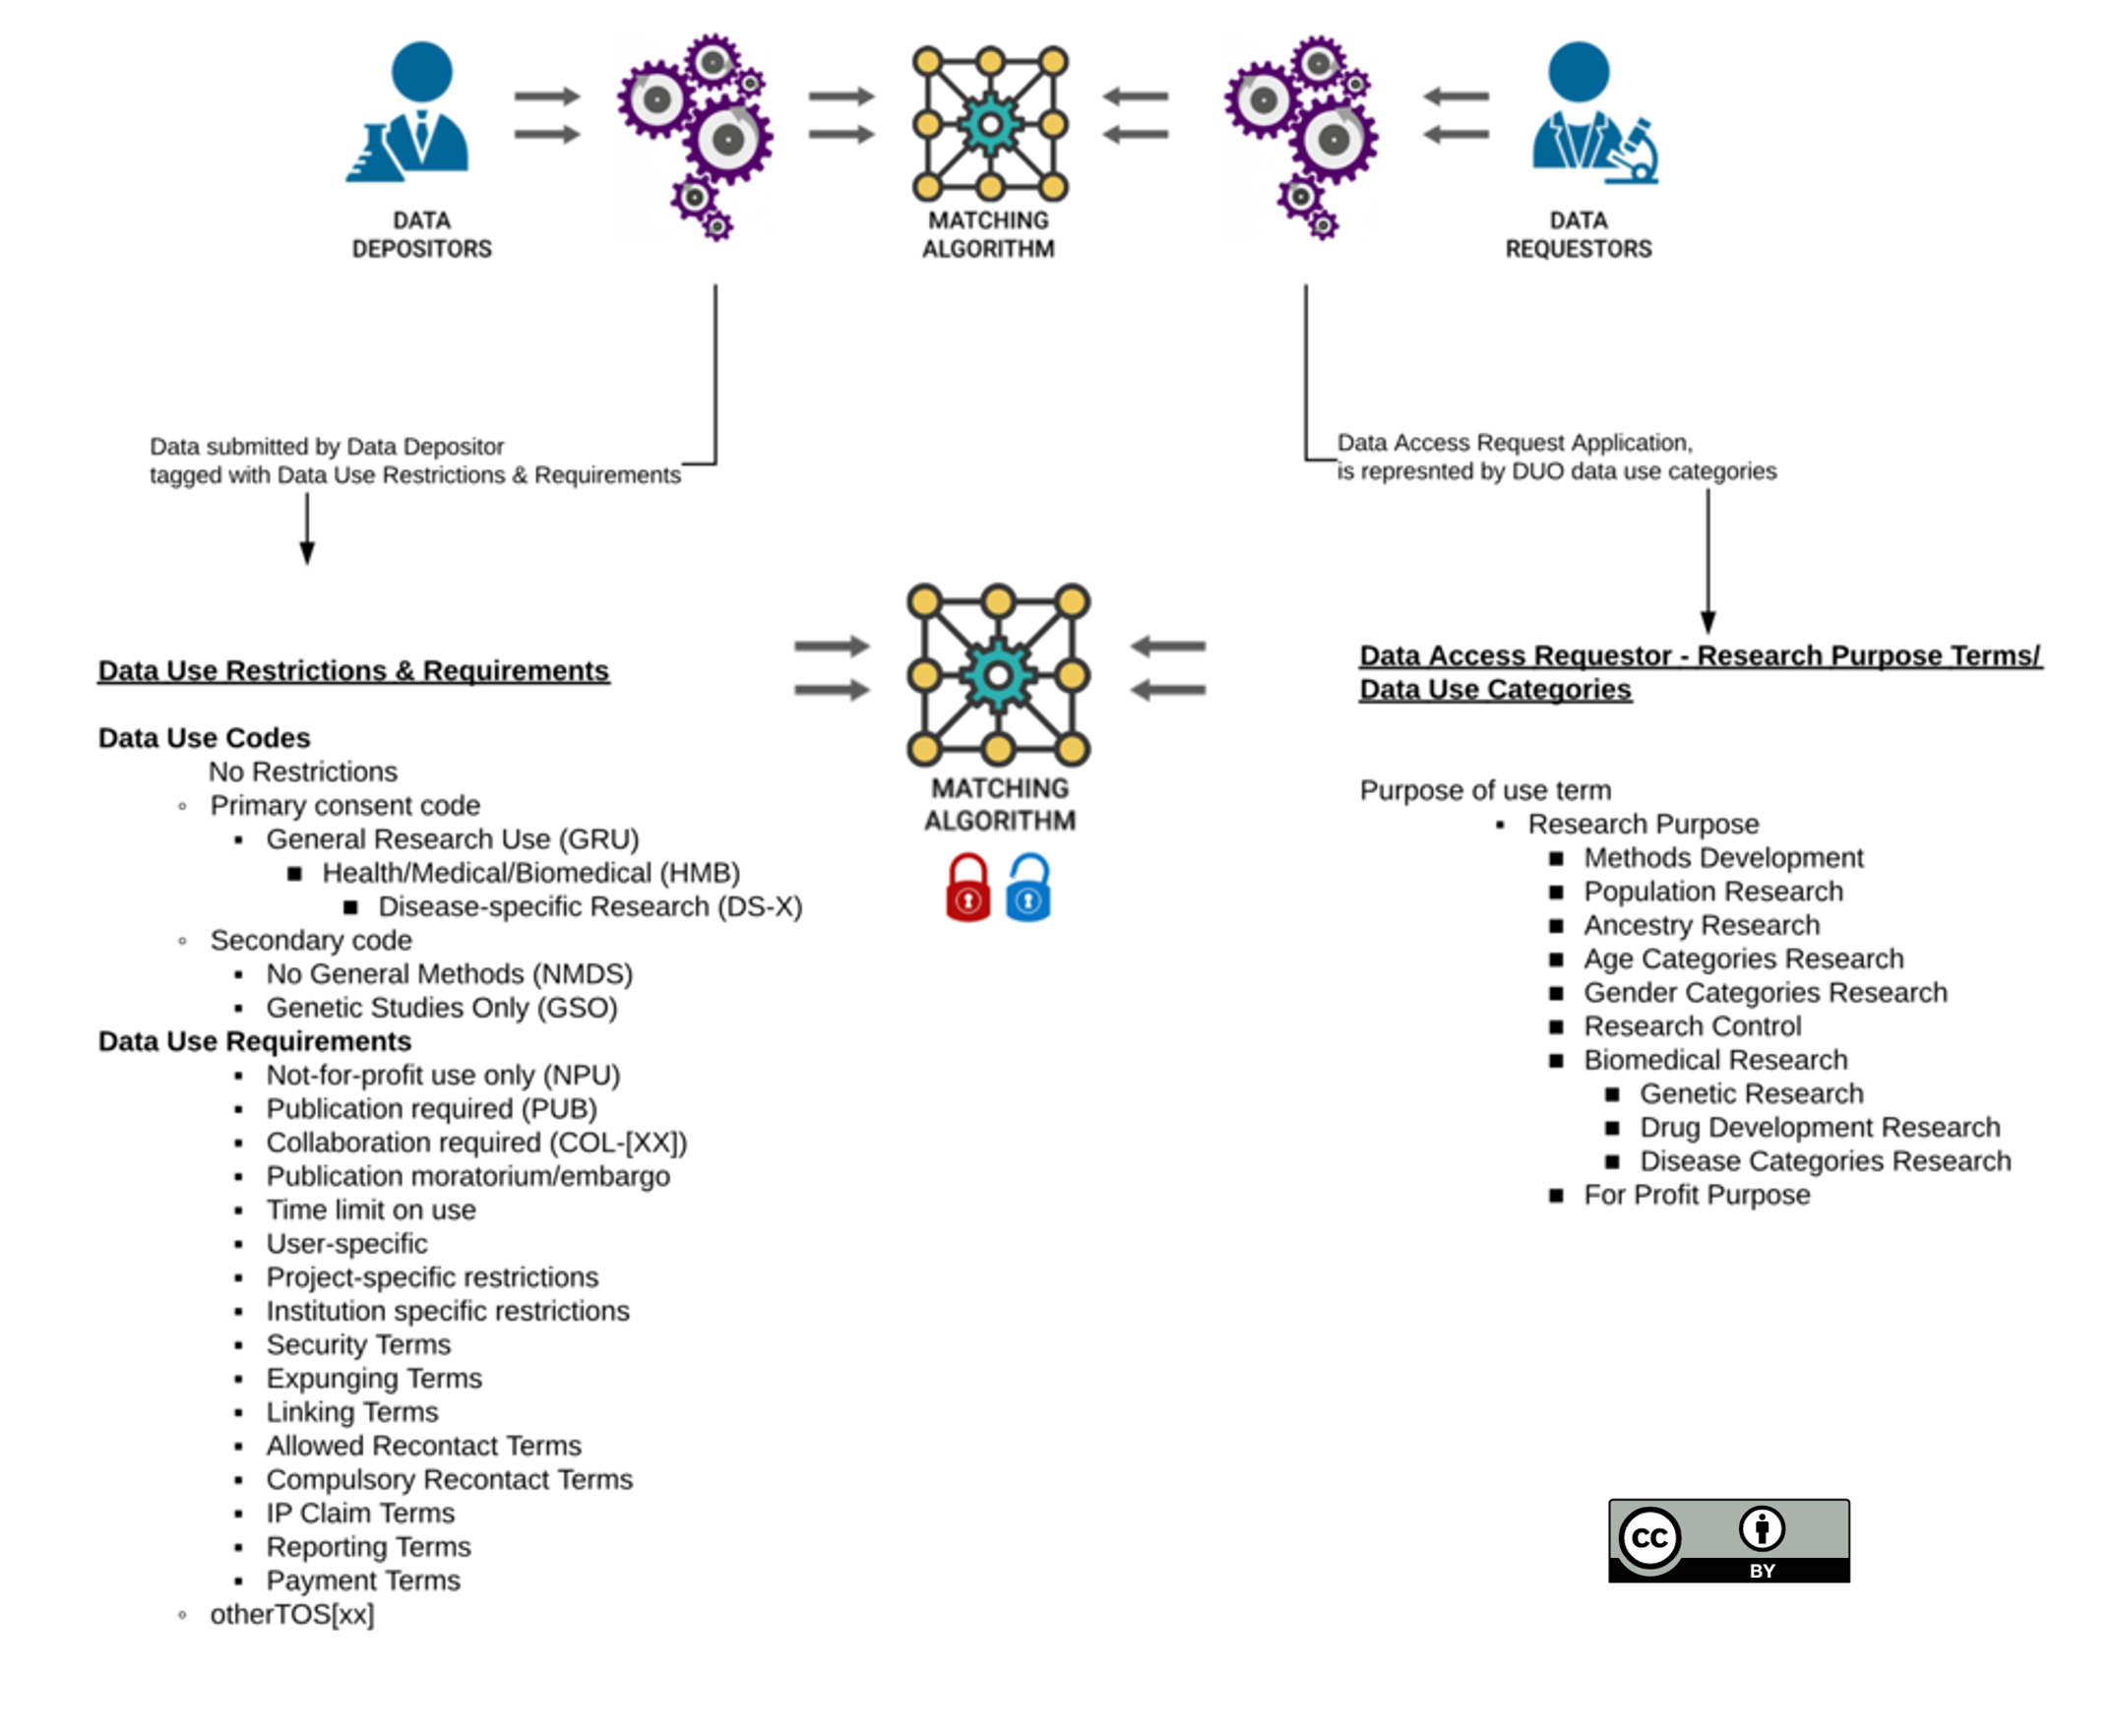
\includegraphics[width=1\linewidth]{figures//chapter-6/DUO-matching-with-license.png}
    \caption[DUO-based matching algorithm.]{DUO-based matching algorithm, adapted from \url{https://github.com/EBISPOT/DUO}.}
    \label{fig:duo-matching}
\end{figure}

Beyond DUOS, the DUO specification has been integrated into various other works, including a specification of informed consent for health and genomics research in Africa \citep{nembaware_framework_2019}, a blockchain-based consent model for health data sharing \citep{jaiman_consent_2020}, and an online platform that offers dynamic consent interfaces and tools for large-scale genomics research programs \citep{haas_ctrl_2021}.
Furthermore, DUO is mentioned in the Data Tags Suite (DATS), where it is considered a candidate vocabulary within its framework for discovering metadata-based data access conditions \citep{alter_data_2020}.
Additionally, it plays a role in the roadmap of European infrastructures for accessing a large number of human genomes  \citep{saunders_leveraging_2019}.
Moreover, \cite{amith_expressing_2022} demonstrate the usage of DUO for the representation of consent metadata, employing SWRL\footnote{\url{https://www.w3.org/Submission/SWRL/} (accessed on 3 April 2024)} to execute permissive rules, and \cite{grabus_landscape_2019} provide a comprehensive overview of rights and licensing initiatives, approaches, and tools for health data sharing, including DUO.

\paragraph{Challenges of the DUO specification}
DUO expresses DULs as concepts with human-readable definitions, utilising the \texttt{obo:IAO\_0000115} property, e.g., as \texttt{skos:definition} is used to define SKOS concepts.
This limits their utility to humans or machines that operate solely on known concepts.
Furthermore, DUO concepts lack linkage to relevant legal concepts, leading to ambiguity regarding the implications of their usage in strongly legislated jurisdictions like the EU, where the GDPR~\citeyearpar{noauthor_regulation_2016} introduces additional accountability and compliance requirements that must be acknowledged and adhered to.
While existing documentation mentions that the applicability of laws falls under the responsibility of the adopter and that DUO terms have not been evaluated for GDPR compliance, it is crucial for data subjects and data controllers to ensure compatibility with existing regulations.
As such, the absence of such support from the DUO specification poses a risk of hindering interoperability as additional approaches need to be taken to fulfil legal requirements.
Moreover, with the EU push to have a common `Health Data Space'\footnote{\url{https://ec.europa.eu/health/ehealth-digital-health-and-care/european-health-data-space_en} (accessed on 2 April 2024)}, machine-readability and automation will play a pivotal role in facilitating legally-aligned health data exchange.

Furthermore, no instructions were found on how to associate DUO conditions with datasets nor on how the data access agreements matching algorithm should work.
While the DUOS framework provides a comprehensive description of how DUO can be utilised, it lacks detailed guidance on the matching algorithm.
DATS \citep{alter_data_2020} also acknowledges the challenge of using DUO for defining permissions and prohibitions, suggesting ODRL as an alternative model for clearer articulation of permissions and prohibitions.

\paragraph{Proposed improvements over the DUO specification}
To achieve \textit{true machine-readability}, DUO concepts must be represented with permissions, prohibitions, constraints, and duties to form machine-readable rules, by leveraging semantic standards for the expression of asset usage conditions.
By formalising the DULs embedded within the descriptions of each DUO concept as a set of rules, these become explicit and can be attached and sent alongside the data for future inspection.

To assess the compatibility of a data request with the dataset's DULs, both the conditions set by the data provider and those articulated by the data requester for data use should be formulated as policies.
These policies can then be matched to determine if the intended use aligns with the dataset's conditions, using the same approach as the one presented in Section~\ref{sec:algorithm}.
While DUO is currently being utilised in this manner, as evidenced in systems like DUOS, the matching relies on hierarchical compatibility between data request and data use conditions established through a subclass relationship, i.e., a data request $DR$ is a subclass/superclass of a data use condition $DUC$.
This approach has limitations in terms of its capacity and expressiveness for delineating fine-grained rules to utilise in automated systems, as not all relevant pieces of information can be explicitly captured in distinct concepts.
For instance, DUO's \texttt{DUO\_0000006} indicates through a sole human-readable label that use is allowed for health/medical/biomedical research purposes, not including the study of population origins or ancestry, while the same information can be much more explicitly declared using ODRL policies with permission and prohibition rules with purpose constraints.

More significantly, in order to automate the generation of data access/usage agreements effectively, a set of criteria should be considered when selecting a vocabulary to articulate such conditions:
\begin{enumerate}
    \item[(i)] the level of expressiveness to define rules and policies, encompassing the ability to express actions, purposes, or other constraints as distinct concepts that can be autonomously specified and evaluated, and combined in distinct ways to represent various types of policies;
    \item[(ii)] the capability to associate and verify their conformity and adherence to legal requirements, e.g., such as the GDPR; and
    \item[(iii)] the capacity to specify access/usage conditions in a machine-readable format and utilise them for assessing the accuracy and comprehensiveness of information that should be in such a data agreement.
\end{enumerate}
% FROM THE PAPER: Such solutions have existed for a while now -- for example, Answer Set Programming (ASP) and logic-based semantic reasoners have been utilised in a variety of domains -- including for representing information and using it for checking legal compliance for GDPR (see Section.\ref{sec:sota-legal}).

With the aforementioned motivation in mind, this Thesis proposes an approach to explicitly represent DUO concepts using RDF, leveraging ODRL and the efforts declared in previous Sections related to an OAC-based architecture for decentralised access to data.
The choice of using ODRL, beyond being a W3C Recommendation for the expression of policies, is supported by the following motives:
\begin{enumerate}
    \item[(i)] it is RDF-based, ensuring machine-readability;
    \item[(ii)] it encompasses concepts that model domain-specific and legally relevant terms to depict constraints, such as spatial and temporal operators, as well as support various types of policies like offers, requests, and agreements; % Additionally, it offers flexibility in utilizing these concepts in a manner analogous to the conventional contents and structures of legal agreements;
    \item[(iii)] its usage can be validated, and efforts are underway within the W3C ODRL CG to actively develop a formal semantics specification~\citep{fornara_odrl_2023};
    \item[(iv)] it facilitates the development of extensions through ODRL profiles, offering the flexibility to tailor ODRL to specific requirements -- as proved by this Thesis' work on OAC (Section~\ref{sec:oac}), which connects ODRL with legal requirements using DPV and can be extended to cater for legal requirements of health data sharing; and
    \item[(v)] backward compatibility can be ensured -- existing DUO-based systems can adopt the practices suggested in this Section and continue being compatible with the DUO specification. Also, DUO users can select which aspects of this solution they want to incorporate into their system.
\end{enumerate}

As such, based on the algorithms described in Section~\ref{sec:algorithm}, in this Section, (i) DUO concepts are modelled as ODRL policies, (ii) such policies are instantiated as ODRL offers for access to health-related datasets, (iii) offers are matched with incoming data requests to generate permissive or prohibitive data agreements, and (iv) work on OAC is recycled to deal with GDPR obligations for the processing of health data.

\subsection{Re-modelling DUO concepts with ODRL}
\label{sec:poc_duodrl}

As outlined in the previous Section, DUO concepts are organised into three taxonomies with textual annotations representing the access conditions.
This Section's main goal is to examine this implicit information and articulate it explicitly as ODRL policies.

Additionally, it aims to ensure compatibility with current and future GA4GH activities, minimising significant disruptions to existing workflows that already use DUO.
% FROM THE PAPER: We consider DUO's primary attractiveness to be the ease with which its concepts can be easily constructed from input mechanisms (such as a form) and simply `tagged' onto a dataset as an annotation. In this, the textual clauses used to describe the concepts are based on well-defined clauses from consent forms\textsuperscript{18}.
Therefore, the role of ODRL is not to supplant DUO but rather to supplement it by providing extra machine-readable information for each DUO concept.
This additional information makes explicit the conditions currently embedded in DUO's textual annotations, enabling them to be validated, matched, and used for data access in an automated fashion.
An ODRL-improved DUO specification can also be used for additional information duties, such as record-keeping by institutions or other legal tasks.
Following the algorithm proposed in Section~\ref{sec:algorithm}, DUO's taxonomies are modelled as ODRL offers and requests and used as inputs of the policy matching algorithm to generate data access agreements.

\paragraph{Identifying ODRL equivalents for DUO concepts}
For each DUO term, the initial task involved discerning the rules and constraints it encompasses, through the analysis of its textual description, to determine whether it should be modelled as a permission, prohibition, or obligation, as well as understanding the specific context in which they should be applied.
With this analysis, the redundancy and overlap between DUO's data use permissions and modifiers is noticeable, as both include purpose-based policies without a clear differentiation in their semantics.
For instance, \texttt{DUO\_0000011} denotes permission, while \texttt{DUO\_0000044} signifies prohibition, both for `population origins or ancestry research' purposes, with the former categorised as a data use permission and the latter a modifier.

Hence, in this Thesis, the restructuring of the DUO taxonomies is proposed by introducing a unique purpose-based taxonomy that models research concepts as ODRL policies, with variants for permissions and prohibitions, and duties applied over permissions with specific research purposes.
% FROM THE PAPER: This is based on DUOS's data collection input forms and ADA-M's concepts where each research purpose can be individually consented (or restricted) to, with possible implications arising from lack of any permission or prohibition.
For instance, the DUO concept for code \texttt{HMB}, which states that ``[t]his data use permission indicates that use is allowed for health / medical / biomedical purposes (HMB); [and] does not include the study of population origins or ancestry'' in its textual definition, should be articulated as being a permission for a purpose of type \texttt{HMB} and not a purpose of type \texttt{POA}.
This approach allows for a more precise expression and application of DUO's \texttt{HMB} concept by revealing its underlying concepts (purpose) and the rules governing it (permission).

Furthermore, upon analysing DUO's concepts and their inherent access conditions, ODRL rules were modelled to represent the conditions of each DUO concept.
In cases where ODRL lacks the necessary concepts, an extension to its existing concepts is proposed to cover the missing ones.
In this context, for each concept, an \texttt{odrl:Set} instance was modelled to represent the DUO concept's intrinsic rules.
These policies are then amalgamated into an \texttt{odrl:Offer}, to serve as a unified policy for a dataset, as detailed in Section~\ref{sec:algorithm-offer} regarding the instantiation of offer policies.
A comprehensive compilation of the performed interpretations for each DUO concept is provided in Table~\ref{tab:DUO_ODRL_overview}.
As will also be mentioned later in this Section, the original DUO concept definitions will still be kept in the interpreted ODRL policies using the \texttt{rdfs:label} property.
Moreover, due to the interpretive nature of this analysis, difficulties were found in interpreting specific expressions such as `is limited to', a term that suggests that usage is restricted solely within a particular scope.
If this interpretation holds true, DUO developers should clarify how potential conflicts arising from rules expressing exclusive limitations versus other permissive expressions, such as `is allowed for', should be resolved.
Hence, in this Thesis, ODRL's capabilities are used to articulate these requirements as permissions, prohibitions, and obligations, and, subsequently, existing works on ODRL~\citep{pellegrini_automated_2018,de_vos_odrl_2019} and OWL~\citep{bonatti_realtime_2020} reasoners can be employed to aid solving conflict resolution issues.

\begin{table}[htp]
\caption{Interpretation of DUO concepts' textual descriptions as ODRL policies.}
\label{tab:DUO_ODRL_overview}
\footnotesize
\resizebox{\textwidth}{!}{%
\begin{tabular}{p{1.7cm}||p{1.2cm}|p{1.45cm}|p{8.6cm}|p{3.1cm}}
Concept & Code & Rule Type & Constraint & Placeholder \\ \hline\hline
DUO0000001 & \multicolumn{4}{l}{\textbf{Data Use Permission}} \\ \hline\hline
DUO0000042 & GRU & Permission & Purpose is :GRU & ~ \\ \hline
DUO0000006 & HMB & Permission & Purpose is :HMB and not :POA & ~ \\ \hline
DUO0000007 & DS & Permission & Purpose is :DS and mondo:0000001 & :TemplateDisease \\ \hline
DUO0000004 & NRES & Permission & Purpose is odrl:Purpose & ~ \\ \hline
DUO0000011 & POA & Permission & Purpose is :POA & ~ \\ \hline
DUO0000011 & POA & Prohibition & Purpose is not :POA & ~ \\ \hline\hline
DUO0000017 & \multicolumn{4}{l}{\textbf{Data Use Modifier}} \\ \hline\hline
DUO0000043 & CC & Permission & Purpose is :CC & ~ \\ \hline
DUO0000020 & COL & Duty & Action is :CollaborateWithStudyPI & ~ \\ \hline
DUO0000021 & IRB & Duty & Action is :ProvideEthicalApproval & ~ \\ \hline
DUO0000016 & GSO & Permission & Purpose is :GS or :GSG & ~ \\ \hline
DUO0000016 & GSO & Prohibition & Purpose is :GS and not :GSG & ~ \\ \hline
DUO0000022 & GS & Permission & Spatial is equal to specified :Location & :TemplateLocation \\ \hline
DUO0000022 & GS & Prohibition & Spatial is not equal to specified :Location & :TemplateLocation \\ \hline
DUO0000028 & IS & Permission & Assignee is :ApprovedInstitution & :TemplateInstitution \\ \hline
DUO0000028 & IS & Prohibition & Assignee is not :ApprovedInstitution & :TemplateInstitution \\ \hline
DUO0000015 & NMDS & Prohibition & Purpose is :MDS & ~ \\ \hline
DUO0000018 & NPUNCU & Permission & Assignee is :NonProfitOrganisation and Purpose is :NCU & ~ \\ \hline
DUO0000018 & NPUNCU & Prohibition & Assignee is :ForProfitOrganisation and Purpose is :NCU & ~ \\ \hline
DUO0000018 & NPUNCU & Prohibition & Assignee is :NonProfitOrganisation and Purpose is not :NCU & ~ \\ \hline
DUO0000046 & NCU & Permission & Purpose is :NCU & ~ \\ \hline
DUO0000046 & NCU & Prohibition & Purpose is not :NCU & ~ \\ \hline
DUO0000045 & NPU & Permission & Assignee is :NonProfitOrganisation & ~ \\ \hline
DUO0000045 & NPU & Prohibition & Assignee is :ForProfitOrganisation & ~ \\ \hline
DUO0000044 & NPOA & Prohibition & Purpose is :POA & ~ \\ \hline
DUO0000027 & PS & Permission & Project is :ApprovedProject & :TemplateProject \\ \hline
DUO0000027 & PS & Prohibition & Project is not :ApprovedProject & :TemplateProject \\ \hline
DUO0000024 & MOR & Duty & Action is odrl:distribute :ResultsOfStudies with odrl:dateTime & :TemplateDateTime \\ \hline
DUO0000019 & PUB & Duty & Action is odrl:distribute :ResultsOfStudies & ~ \\ \hline
DUO0000012 & RS & Permission & Purpose is specified :Research & :TemplateResearch \\ \hline
DUO0000012 & RS & Prohibition & Purpose is not specified :Research & :TemplateResearch \\ \hline
DUO0000029 & RTN & Duty & Action is :ReturnDerivedOrEnrichedData & ~ \\ \hline
DUO0000025 & TS & Permission & Time is less than specified :TemplateDateTime & :TemplateDateTime \\ \hline
DUO0000026 & US & Permission & Assignee is :ApprovedUser & :TemplateUser \\ \hline
DUO0000026 & US & Prohibition & Assignee is not :ApprovedUser & :TemplateUser \\ \hline\hline
OBI0000066 & \multicolumn{4}{l}{\textbf{Investigation}} \\ \hline\hline
DUO0000034 & & Permission & Purpose is :AgeCategoryResearch & \\ \hline
DUO0000034 & & Permission & Age is specified :Age & :TemplateAgeCategory \\ \hline
DUO0000033 & ~ & Permission & Purpose is :POA & \\ \hline
DUO0000037 & ~ & Permission & Purpose is :HMB & \\ \hline
DUO0000040 & ~ & Permission & Purpose is :DS and mondo:0000001 & :TemplateDisease \\ \hline
DUO0000039 & ~ & Permission & Purpose is :DrugDevelopment & \\ \hline
DUO0000038 & ~ & Permission & Purpose is :GS & \\ \hline
DUO0000035 & ~ & Permission & Purpose is :GenderCategoryResearch & \\ \hline
DUO0000035 & & Permission & Gender is specified :Gender & :TemplateGender \\ \hline
DUO0000031 & ~ & Permission & Purpose is :MDS & \\ \hline
DUO0000032 & ~ & Permission & Purpose is :PopulationGroupResearch & \\ \hline
DUO0000032 & & Permission & Population is specified :Population & :TemplatePopulation \\ \hline
DUO0000036 & ~ & Permission & Purpose is :ResearchControl & \\
\end{tabular}}
\end{table}

Presently, DUO concepts are confined to delineating conditions for data use, suggesting the usage of external ontologies to incorporate additional concepts needed for refining the scope of the term, e.g., \texttt{DUO\_0000007} denotes permission for disease-specific research and recommends the usage of the Mondo Disease Ontology ontology\footnote{\url{https://obofoundry.org/ontology/mondo} (accessed on 4 April 2024)} for specifying the diseases to which the permission applies. 
Other specific concepts mentioned in DUO's textual annotations, which are not explicitly modelled, include codes inherited from previous iterations of DUO, such as purpose terms like \textit{CC} for Clinical Care Use, or \textit{GRU} for General Research Use.
To express ODRL policies, these concepts need an explicit, individual semantic specification, so that they can be used to constrain permissions or prohibitions.
Thus, in this Thesis' implementation, missing terms were identified and compiled into an ad-hoc vocabulary (DUODRL\footnote{DUODRL is published at \url{https://w3id.org/duodrl}.}) to enable the correct expression of ODRL policies for each DUO concept.
% \beatriz{generate documentation for DUODRL and update w3id. }
% FROM THE PAPER: We recommend DUO to adopt these or to create a similar vocabulary for explicitly providing the concepts and their descriptions separate from the data use conditions in which they are used. 
This approach also offers the benefit of delivering more comprehensive documentation related to the information represented within DUO concepts.
For instance, by modelling \textit{IRB} as an ODRL policy representing the duty to get an Ethics Review Board approval, instead of just using the DUO concept, it becomes feasible to include details about the processes and requirements necessary for such reviews.
It also allows additional constraints related to ethics approvals to be semantically linked with this foundational concept, such as indicating that it must be conducted before data access is provided, periodically, or before any outcomes of the research are published.

In the case of data requests, the so-called DUO `Investigations', redundant concepts were found in relation to both the data use permissions and modifiers concepts, e.g., \texttt{DUO\_0000040} denotes a data request for research on a specific disease, while \texttt{DUO\_0000007} signifies permission for research on a specific disease.
In essence, both concepts convey the same idea concerning `research on a specific disease', albeit with one indicating a data request and the other representing the dataset's permissive conditions.
As such, as previously suggested in relation to the reorganisation of DUO's `Data Use Permission' and `Data Use Modifier' taxonomies to be research purpose-based, a similar approach should be adopted for data requests to ensure consistency in the concepts used for requesting data.
This alignment promotes clarity, reduces ambiguity, and facilitates the matching process, as the same rules can be associated to a dataset through an \texttt{odrl:Offer} and to a data request through an \texttt{odrl:Request}.

Besides specifying requirements for data access and requests to access said data, DUO concepts should also be utilised to document the result of the matching algorithm, and whether access is to be granted or not.
This aspect represents an important yet unexplored domain in the current identified applications of DUO, particularly because any data sharing typically entails accompanying information about the involved parties, the provenance linked with the granting process, and details regarding how the data access conditions were satisfied at the time or what are future duties for the access to be granted.
Hence, the work on this Thesis related to the generation of data access agreements, described in detail in Section~\ref{sec:algorithm-agreement}, will be beneficial in portraying this information, not to mention the work on OAC and PLASMA, which can encompass all the aforementioned policy and metadata-related details.
Furthermore, these agreements can be employed in automated processes that periodically verify if the pending duties on an agreement still have to be or are already fulfilled, e.g., the publication of the research results.

\paragraph{DUO concepts as \texttt{odrl:Set}s}
Considering the points raised above, every DUO restriction should be portrayed as a \texttt{odrl:Set} instance, which, according to its definition, should include at least one permission, prohibition, or obligation, along with one associated data asset, to be deemed a semantically correct ODRL policy.
Its utilisation does not confer any access privileges but solely denotes a set of rules that are applicable to the resource.
Considering the human-readable labels linked with each DUO concept, \texttt{odrl:permission} was used when the condition permitted access to data, \texttt{odrl:prohibition} when it prohibited access, and \texttt{odrl:duty} when it outlined obligations to allow data access. 
DUO's textual descriptions are still kept in the policies via the \texttt{rdfs:label} property and the connection with the original DUO concept using \texttt{skos:exactMatch}.

Constructing a valid ODRL policy proved challenging due to the necessity of specifying \textit{``any form of identifiable resource''}~\citep{iannella_odrl_vocab_2018}.
This challenge arises because DUO concepts solely represent specific access and usage requirements unrelated to a specific dataset.
Additionally, DUO does not indicate how to express values associated with requirements such as research in specific diseases or temporal duration of access.
To ensure the validity of ODRL policies and provide clarity on how to later apply or instantiate them as an \texttt{odrl:Offer} for a particular dataset, the base class \texttt{TemplateQuery} was introduced in DUODRL.
Instances of this class serve as a placeholder to be substituted with the actual value(s) obtained by executing a SPARQL query which is linked with the placeholder through the \texttt{sparqlExpression} property.
In Table~\ref{tab:DUO_ODRL_overview}, these instances are denoted in the `Placeholder' column.
Examples of this approach are illustrated in Listing~\ref{list:duodrl_set} for an \texttt{odrl:Set} representing a DUO data use permission and a modifier.
In this case, the placeholders are employed to indicate datasets that are not instantiated yet and a publication date that is still not determined.
These placeholders can be later replaced with actual instances in real policies, e.g., by utilising SPARQL queries.

The indication of scoped restrictions, such as specifying the geographic location when use is confined to a particular region, was also not void of issues.
Within DUO, the \texttt{obo:DUO\_0000010} property is used to describe a `is restricted to' relationship, which is intended to specify the specific values or instances of variables such as diseases or locations.
However, the descriptions of DUO concepts only mention that \textit{``this should be coupled with an ontology term describing the (concept) the restriction applies to''}, without providing an example illustrating how it should be utilised.

Hence, to address this challenge, four possible approaches were identified:
\begin{enumerate}
    \item [(i)] utilising OWL class expressions\footnote{\url{https://protegeproject.github.io/protege/class-expression-syntax/} (accessed on 6 April 2024)};
    \item [(ii)] employing SHACL shapes to specify a constraint;
    \item [(iii)] developing a new ODRL \texttt{Operator} that accepts property paths; or
    \item [(iv)] directly stating the term as an instance of the scoping concept, e.g., for disease-specific restrictions, the concept would be instantiated as both the appropriate DUO concept and the disease concept).
\end{enumerate}
Each of these approaches influences how a condition is articulated and impacts the performance and functionality of the policy matching algorithm, e.g., leveraging approach (i) would necessitate the execution of an OWL2 reasoner before the matching process, while approach (ii) would require a SHACL validator.
In this Thesis, the fourth approach was taken by declaring the concept as an instance of both the DUO and the scoping classes.
This method was chosen for its simplicity and absence of the need for additional tools or modifications to ODRL.
Moreover, if no extra tools or modifications are needed and a different method in the future is found to be more effective then it can easily replace the one proposed in this Section.
Additionally, by reusing the existing ODRL and OAC models, it is also possible to reuse the algorithms specified in Section~\ref{sec:algorithm}.

The \texttt{odrl:Set} formulated to represent DUO's concept of \textit{``general research use''} and the one to represent DUO's concept of \textit{``publication moratorium''} are detailed in Listing~\ref{list:duodrl_set}.
When instantiated, beyond additional provenance metadata such as the \texttt{dcterms:creator} and \texttt{dcterms:issued} properties to indicate the creator and date of issuance of the offer, the\linebreak \texttt{duodrl:TemplateDataset} must be replaced by the dataset's identifier and, in the case of the moratorium, a date must be instantiated to express until when the distribution of the outcomes of the research study is prohibited. 

\begin{listing}[htp]
\caption[\texttt{odrl:Set}s representing DUO's GRU and MOR concepts.]{\texttt{odrl:Set}s representing \texttt{DUO\_0000042}, a data use permission for general research purposes (GRU), and \texttt{DUO\_0000024}, a data use modifier to indicate that the results of the research should be published only after a moratorium period (MOR).}
\label{list:duodrl_set}
\begin{minted}{turtle}
duodrl:DUO_0000042 a odrl:Set ;
    odrl:uid duodrl:DUO_0000042 ;
    odrl:profile oac: ;
    rdfs:label "DUO_0000042: This data use permission indicates that use is allowed for general research use for any research purpose (GRU - general research use)"@en ;
    skos:exactMatch obo:DUO_0000042 ;
    skos:editorialNote "We interpreted this as a permission for a research purpose that is an instance of general research purposes (GRU). We note that the DUO concept description consists of specific areas of research which can be additionally indicated if meant as an exclusive list, i.e., purpose must be one of those, or provide as subclasses of GRU if meant to be provided as a selection, i.e., purpose can be expressed as one of those"@en ;
    odrl:permission [
        odrl:action odrl:use ;
        odrl:target duodrl:TemplateDataset ;
        odrl:constraint [
            odrl:leftOperand oac:Purpose ;
            odrl:operator odrl:isA ;
            odrl:rightOperand duodrl:GRU ] ] .
    
duodrl:DUO_0000024 a odrl:Set ;
    odrl:uid duodrl:DUO_0000024 ;
    rdfs:label "DUO_0000024: This data use modifier indicates that requestor agrees not to publish results of studies until a specific date (MOR - publication moratorium)"@en ;
    skos:exactMatch obo:DUO_0000024 ;
    skos:editorialNote "We interpret this as a prohibition to not publish results until the specified date as indicated by TemplateStudyResultsPublicationDate placeholder. We also note that this rule may be expressed using odrl:delayPeriod or odrl:dateTime if it should be expressed as a (delayed) permission to publish instead of a prohibition"@en ;
    odrl:prohibition [
        odrl:target duodrl:TemplateDataset ;
        odrl:action odrl:distribute ;
        odrl:output duodrl:ResultsOfStudies ;
        odrl:constraint [
            odrl:leftOperand odrl:dateTime ;
            odrl:operator odrl:lt ;
            odrl:rightOperand duodrl:TemplateStudyResultsPublicationDate ] ] .
\end{minted}
\end{listing}

\paragraph{Dataset policies as \texttt{odrl:Offer}s}
Datasets can be annotated with several DUO concepts.
In this context, an instantiation algorithm must be used to collect the \texttt{odrl:Set}s that should be applied to the dataset to be instantiated into an \texttt{odrl:Offer}.
For this, the algorithm for offer instantiation presented in Section~\ref{sec:algorithm-offer} can be recycled for the particular use case of DUO.
As such the following steps were taken to instantiate dataset policies as \texttt{odrl:Offer}s:
\begin{enumerate}
    \item For a given dataset, retrieve all data use permissions and data use modifiers that the dataset was tagged with.
    \item Filter out duplicated policies.
    \item If a retrieved policy contains instances of \texttt{TemplateQuery}, e.g., \texttt{TemplateDataset}, execute their SPARQL queries to replace the template with the retrieved values.
    \item For each retrieved policy, fetch relevant \texttt{odrl:Permission} and \texttt{odrl:Prohibition} rules and merge them in a single \texttt{odrl:Offer}.
    \item A link to each `original' policy is maintained in the final \texttt{odrl:Offer} by using the \texttt{dcterms:source} property.
    \item Add provenance information to the \texttt{odrl:Offer}, e.g. \texttt{dcterms:issued} for when the offer was instantiated and \texttt{dcterms:creator} for the issuer of the policy.
\end{enumerate}

An example \texttt{odrl:Offer}, which merges the \texttt{DUO\_0000042}, \texttt{DUO\_0000025} and\linebreak \texttt{DUO\_0000020} policies as conditions to access the \texttt{ex:EHR} dataset, is presented in Listing \ref{list:duodrl_offer}.

\begin{listing}[ht]
\caption[\texttt{odrl:Offer} containing DUO's GRU, TS and COL concepts.]{An example \texttt{odrl:Offer} containing a permission for general research use (GRU), from \texttt{DUO\_0000042}, a time limit on the use (TS), from \texttt{DUO\_0000025}, and a duty to collaborate with the studies' primary investigator (COL), defined from \texttt{DUO\_0000020}.}
\label{list:duodrl_offer}
\begin{minted}{turtle}
ex:offer_for_GRU_TS_COL a odrl:Offer ;
    odrl:uid ex:offer_for_GRU_TS_COL ;
    odrl:profile oac: ;
    rdfs:label "Offer to use dataset for GRU within time limits while collaborating with the primary study investigator" ;
    odrl:assigner ex:provider ;
    odrl:target ex:EHR ;
    odrl:action odrl:use ;
    dcterms:source duodrl:DUO_0000042, duodrl:DUO_0000025, duodrl:DUO_0000020 ;
    dcterms:issued "2024-04-06"^^xsd:date ;
    odrl:permission [
        odrl:duty [ odrl:action duodrl:CollaborateWithStudyPI ] ] ;
    odrl:permission [
        odrl:constraint [ 
            odrl:leftOperand odrl:elapsedTime ;
            odrl:operator odrl:lteq ;
            odrl:rightOperand "2024-12-31"^^xsd:date ] ] ;
    odrl:permission [
        odrl:constraint [ 
            odrl:leftOperand oac:Purpose ;
            odrl:operator odrl:isA ;
            odrl:rightOperand duodrl:GRU ] ] .
\end{minted}
\end{listing}

Moreover, in decentralised data environments, the discovery of the dataset's location will play an important role as during the offer instantiation algorithm the \texttt{TemplateDataset} variable must be substituted by the real location of the dataset to which the offer applies.
As such, the SPARQL query identified in Listing~\ref{list:sparql_duodrl} showcases an example of how to find the location of medical health data datasets, tagged as such using the DPV's personal data categories extension, and in particular the \texttt{pd:MedicalHealth} term, and using the PLASMA conforming specification of a data registry.
By running such a query it will be possible to find the location of specific datasets in decentralised settings such as the ones promoted by Solid.
Similar queries can also be executed for decentralised environments beyond Solid or even within centralised environments.

\begin{listing}[ht]
\caption[SPARQL query to retrieve datasets location from PLASMA data registry.]{SPARQL query to retrieve template datasets locations from a PLASMA data registry specified in a Solid Pod.}
\label{list:sparql_duodrl}
\begin{minted}{sparql}
SELECT DISTINCT ?DatasetsLocation WHERE {
    ?DataRegistry a plasma:DataRegistry .
    ?DataRegistry dcat:catalog ?Entry .
    ?Entry a dcat:Catalog .
    ?Entry dcat:themeTaxonomy pd:MedicalHealth .
    ?Entry dcat:dataset ?DatasetsLocation .
}
\end{minted}
\end{listing}

\paragraph{Data access outcomes as \texttt{odrl:Agreement}s}
To provide access to a dataset, data-handling environments must be able to match dataset policies with a specific request being made e.g. for research with health data.
For this, DUO's requests must be instantiated as \texttt{odrl:Request}s to be matched with the datasets \texttt{odrl:Offer}s.
A request for health, medical, or biomedical research studies (\texttt{DUO\_0000037}) is presented in Listing~\ref{list:duodrl_request}.

\begin{listing}[htp]
\caption[\texttt{odrl:Request} containing DUO's HMB concept.]{An \texttt{odrl:Request} containing a request for health, medical, or biomedical research (HMB) created from \texttt{DUO\_0000037}.}
\label{list:duodrl_request}
\begin{minted}{turtle}
ex:request_for_HMB a odrl:Request ;
    odrl:uid ex:request_for_HMB ;
    odrl:profile oac: ;
    rdfs:comment "Request for health, medical, or biomedical research" ;
    dcterms:source duodrl:DUO_0000037 ;
    dcterms:issued "2024-05-01"^^xsd:date ;
    odrl:permission [
        odrl:action odrl:use ;
        odrl:target duodrl:TemplateDataset ;
        odrl:assignee ex:requester ;
        odrl:constraint [
            odrl:leftOperand oac:Purpose ;
            odrl:operator odrl:isA ;
            odrl:rightOperand duodrl:HMB ] ] .
\end{minted}
\end{listing}

In this context, an algorithm must be used to collect the conditions under which access to data is allowed/denied.
As such, the algorithm for policy matching presented in Section~\ref{sec:algorithm-agreement} can be recycled for the particular use case of DUO matching for health datasets.
Considering this, the following steps were taken to instantiate dataset access agreements as \texttt{odrl:Agreement}s:

\begin{enumerate}
    \item Retrieve the data requester's \texttt{odrl:Request} and the dataset's \texttt{odrl:Offer}.
    \item Match the \texttt{odrl:Offer} with the \texttt{odrl:Request}.
    \item Record the outcome of the matching algorithm, where the \texttt{odrl:target} property specifies the dataset to be accessed, and the \texttt{odrl:assignee} and \texttt{odrl:assigner} properties identify the data requester and the provider, respectively.
    \item If the matching result is positive, i.e., the request and the offer are compatible, then access is permitted by employing a permission with constraints on the requested purpose for access, along with any additional constraints such as spatial or temporal constraints or duties on the requester. If access is denied, similar information is included in the policy as a prohibition.
    \item Utilise the \texttt{dcterms:references} property to associate the agreement with the\linebreak \texttt{odrl:Offer} and \texttt{odrl:Request} that were used to generate it.
    \item Include provenance and other relevant information, such as the \texttt{dcterms:issued} property, to document the creation and acceptance of the agreement among the parties.
\end{enumerate}

Following these steps, an agreement for access to data can be reached.
An example representation of a DUO-based data access agreement, modelled as an \texttt{odrl:Agreement}, to give access to data until 2024--12--31 for the purpose of health, medical, or biomedical research studies is presented in Listing~\ref{list:duodrl_agreement}, including also a duty which must be fulfilled after data access.

\begin{listing}[htp]
\caption[\texttt{odrl:Agreement} representing an access decision.]{An \texttt{odrl:Agreement} representing a decision to access a \texttt{ex:EHR} dataset from \texttt{ex:provider}.}
\label{list:duodrl_agreement}
\begin{minted}{turtle}
ex:agreement_for_HMB a odrl:Agreement ;
    odrl:uid ex:agreement_for_HMB ;
    odrl:profile oac: ;
    dcterms:references ex:offer_for_GRU_TS_COL, ex:request_for_HMB ;
    dcterms:issued "2024-05-01"^^xsd:date ;
    odrl:action odrl:use ;
    odrl:target ex:EHR ;
    odrl:assigner ex:provider ;
    odrl:assignee ex:requester ;
    odrl:permission [
        odrl:constraint [
            odrl:and ex:constraint_purpose, ex:constraint_temporal ] ;
        odrl:duty [ odrl:action duodrl:CollaborateWithStudyPI ] ] .

ex:constraint_purpose a odrl:Constraint ;
    odrl:leftOperand oac:Purpose ;
    odrl:operator odrl:isA ;
    odrl:rightOperand duodrl:HMB .

ex:constraint_temporal a odrl:Constraint ;
    odrl:leftOperand odrl:elapsedTime ;
    odrl:operator odrl:lteq ;
    odrl:rightOperand "2024-12-31"^^xsd:date .
\end{minted}
\end{listing}

As previously mentioned in the policy matching algorithm described in Section~\ref{sec:algorithm-agreement}, the matching process described in step 2 of agreement generation operates by comparing and assessing the compatibility between the conditions described in dataset policies and in data requests.
Since DUO matching systems are supposed to match offers with requests using subsumption as a criterion, the Algorithm~\ref{alg:matching}, proposed for OAC-based systems in the previous Section, can also be adapted here for the specific use case of DUO-based health data-sharing. 
In DUO's case, for a class $P$ and its subclass $C$, a request to access $P$ does not allow access to $C$ since $C$ is more specific than $P$.
However, a request to access $C$ would allow use of $P$ as $P$ is less specific than $C$.
In light of these considerations, Algorithm~\ref{alg:duodrl_matching} offers pseudo-code that showcases the adapted steps of the policy matching algorithm for the DUO health data use case.

\begin{algorithm}[ht]
\caption{Pseudo-code of the proposed matching algorithm for DUODRL.}
\label{alg:duodrl_matching}
\begin{algorithmic}
\For{$prohibition \gets odrl{:}Offer$}
    \If{$odrl{:}assignee \in offer{:}prohibition$}
        \If{$offer{:}assignee \equiv request{:}assignee$}
            $decision \gets DENY$
        \EndIf
    \EndIf
    \For{$constraint \gets prohibition$}
        \If{$odr{:}spatial \gets constraint$}
            \If{$offer{:}spatial \cap request{:}spatial \neq\emptyset$}
                $decision \gets DENY$
            \EndIf
        \ElsIf{$duodrl{:}Project \gets constraint$}
            \If{$request{:}project \cap offer{:}project \neq\emptyset$}
                $decision \gets DENY$
            \EndIf
        \ElsIf{$odrl{:}dateTime \gets constraint$}
            \If{$timeNow < moratoriumDate$}
                $decision \gets DENY$
            \EndIf
        \ElsIf{$offer{:}purpose \cap request{:}purpose \neq\emptyset$}
            $decision \gets DENY$
        \EndIf
    \EndFor
\EndFor

\For{$permission \gets odrl{:Offer}$}
    \If{$odrl{:}assignee \in offer{:}permission$}
        \If{$offer{:}assignee \not\equiv request{:assignee}$}
            $decision \gets DENY$
        \EndIf
    \EndIf 
    \For{$constraint \gets permission$}
        \If{$odrl{:}dateTime \gets constraint$}
            \If{$timeNow > timeLimit$}
                $decision \gets DENY$
            \EndIf 
        \ElsIf{$request{:}purpose \in groupResearchPurposes$}
            \If{$request{:}purpose \not\subseteq offer{:}purpose \bigvee request{:}group \not\subseteq offer{:}group$}
                $decision \gets DENY$
            \EndIf
        \ElsIf{$request{:}purpose \not\subseteq offer{:}purpose$}
            $decision \gets DENY$
        \EndIf 
    \EndFor 
\EndFor

\If{$ \nexists DENY$}
    $decision \gets GRANT$
\EndIf
\end{algorithmic}
\end{algorithm}

In this context, it is important to note that this algorithm offers a general outline of actions, since DUO's documentation lacks specific details for accurately interpreting certain semantic aspects.
Since this interpretation significantly influences decision-making within DUO's processes, and DUO only specifies how to interpret purposes and not other restrictions, e.g., location, users, projects, this is as an area that might require further exploration and investigation in the future as more details about DUO's matching process are known.
To address this information gap, apart from the purposes in DUO's concepts, the matching of the remaining concepts is performed according to the proposed Algorithm~\ref{alg:matching}, as this proposal considers a legally relevant interpretation of hierarchical concepts, where a narrower concept cannot be deemed compatible with a request for a broader concept, e.g., a permission to access the data within a certain city cannot be fulfilled by a request for a region broader than that city.
Hence, the proposed algorithm mirrors the previously described algorithm for OAC.
Firstly, the prohibitive statements are matched, and only if no incompatibilities are found are the permissions considered.
The denial of the access request occurs during prohibition checking if any of the following restrictions in the dataset offer are found to be incompatible with the data request:

\begin{enumerate}
    \item offer assignee matches ($\equiv$) the request assignee; 
    \item offer has a spatial constraint matching or not satisfying ($\cap\neq\emptyset$) the spatial constraint in the request;
    \item offer has a project constraint matching ($\cap\neq\emptyset$) the project in the request;
    \item there is a moratorium period with a date in the future; and 
    \item offer has a purpose matching ($\cap\neq\emptyset$) the purpose in the request.
\end{enumerate}

If no prohibitions are identified, the next step is to verify the permissions.
Access will be denied during permission checking if any of the following constraints in the request are incompatible with the dataset offer:

\begin{enumerate}
    \item offer assignee does not match ($\not\equiv$) the assignee of the request; 
    \item offer time limit on use has lapsed;
    \item offer has a group-related research purpose, e.g., \texttt{PopulationGroupResearch},\linebreak \texttt{AgeCategoryResearch} or \texttt{GenderCategoryResearch} and the request purpose does not match ($\not\subseteq$) it or the request purpose matches it but the group does not ($\not\subseteq$), e.g. the \texttt{PopulationGroup}, \texttt{Age} or \texttt{Gender} in the request are different from the one in the offer; and
    \item offer purpose does not match ($\not\subseteq$) request purpose, e.g., DUO's general research use purpose \texttt{GRU} in a request does not match a health, medical or biomedical research purpose \texttt{HMB} in an offer as \texttt{GRU} is a superclass of \texttt{HMB}.
\end{enumerate}

The described procedures are applied to all permissions and prohibitions outlined in the dataset's offer.
If all permissions and prohibitions are met without any violations, access to the health-related data can be authorised, if not the \texttt{odrl:Agreement} will include a prohibition that states the motives for the denial of the request.
The proof-of-concept implementation outlined in Section~\ref{sec:poc_implementation} applies these steps to match an offer with request policies in order to generate a data access agreement.

Table~\ref{tab:duodrl_matching_examples} illustrates examples of how the matching algorithm operates for prohibitions and permissions in offers with spatial and purpose-based constraints.
As previously mentioned, in a semantic-based context, performing equivalence ($\equiv$), intersection ($\cap$), and subset ($\subseteq$) checking requires supplementary deliberations beyond simply employing \texttt{owl:sameAs} or \texttt{rdfs:subClassOf} inferences.
For instance, comparing an offer with a location constraint restricted to Spain with a request to Europe using the subset ($\subseteq$) operator for permissions or the intersection ($\cap$) operator for prohibitions needs both locations to be articulated in a manner that facilitates such a hierarchical interpretation.
In this scenario, the matching process requires understanding that \textit{Spain} is a narrower concept, geographically speaking, than \textit{Europe}.
Further complexities arise when representing legal jurisdictions, such as the \textit{EU}, of which \textit{Spain} is a member.

\begin{table}[ht]
\centering
\caption{Examples of outcomes of the policy matching algorithm for DUODRL.}
\label{tab:duodrl_matching_examples}
\resizebox{\textwidth}{!}{%
\begin{tabular}{c|c|c||c|c||c|c}
\multicolumn{3}{c||}{\textbf{Offer}} & \multicolumn{2}{c||}{\textbf{Request}} & \multicolumn{2}{c}{\textbf{Outcome}} \\
\hline
Rule & Purpose & Location & Purpose & Location & Decision & Reason \\
\hline\hline
Permission & GS & Spain & GS & Europe & DENY & Europe $\not\subseteq$ Spain \\
\hline
Permission & GS & Europe & GS & Spain & GRANT & Spain $\subseteq$ Europe \\
\hline
Prohibition & GS & Spain & GS & Europe & DENY & Europe $\cap$ Spain $\neq\emptyset$ \\
\hline
Prohibition & GS & Europe & GS & Spain & DENY & Spain $\cap$ Europe $\neq\emptyset$ \\
\hline
Prohibition & GS & UK & GS & Spain & GRANT & Spain $\cap$ UK $=\emptyset$ \\
\hline
Permission & HMB & ~ & DS-Cancer & ~ & GRANT & DS-Cancer $\subseteq$ HMB \\
\hline
Prohibition & DS-Cancer & ~ & HMB & ~ & DENY & HMB $\cap$ DS-Cancer $\neq\emptyset$ \\
\end{tabular}}
\end{table}

\paragraph{Expressing legal compliance with OAC}
The terminologies and concepts employed in DUO differ significantly from those utilised in legal compliance tasks, e.g., such as the ones mandated by the GDPR.
With the proposed DUODRL approach which leverages ODRL concepts, the terminologies involved are specified in a language which can be legally interpreted, e.g., such as the \texttt{Asset} or \texttt{Party} terms.
Moreover, the ODRL vocabulary encompasses complementary terms that could extend DUO with precise legal annotations, such as the \texttt{odrl:consentingParty}, \texttt{odrl:informedParty}, and \texttt{odrl:obtainConsent} terms.
While these terms suffice for endowing a legally-aligned policy, they may not adequately encompass the specific requirements of laws such as the GDPR, which assigns distinct roles to entities and mandates the use of specific legal grounds for the processing of personal data, including additional requirements for special categories of such data, e.g., such as health data.
Simultaneously, tailoring the terms solely for a single jurisdiction could confine the usefulness and applicability of the proposed work solely to that law, without providing a clear pathway for accommodating other laws and jurisdictions.
To bridge this divide, this Thesis proposes the usage of the OAC profile, which provides legally-aligned terms designed to be jurisdiction-agnostic and adaptable across various legal frameworks.

The work on OAC can be seamlessly integrated into this use case as it already aligns ODRL terms with DPV terms for the expression of legally-aligned policies.
Using OAC, and by consequence DPV, enables the modelling of policies with constraints on the legal basis used to process the data, e.g., consent, or on the third party recipients of the results of the processing, as well as explicitly define the entities processing the data -- the data controllers -- and the data protection laws that must be respected.
The \texttt{oac:TechnicalOrganisationalMeasure} constraint left operand can also be used to ensure that certain measures are taken before or after data access, e.g., impact assessments or records of activities.
To explicitly designate GDPR as the law applicable to the policy and rely on its legal bases for processing, DPV's GDPR extension can be used.
Through this segregation (between DPV and its GDPR extension), policies can be articulated in a jurisdiction-agnostic way, and subsequently tailored to a specific law such as GDPR by factoring in additional contextual information, such as the locations of patients whose data is implicated or the identity of the legal representative the requesting data controller.
This separation also paves the way for applying other laws, within or outside of the EU, which would be possible by crafting other law extensions to DPV akin to developed GDPR one.
Listing \ref{list:duodrol_dpv} provides two ODRL offer policies: the first uses DPV to enact jurisdiction-agnostic data protection terms and the second uses the GDPR extension to describe GDPR-specific terms.

\begin{listing}[htp]
\caption[\texttt{odrl:Offer}s for DUO that use DPV and its GDPR extension.]{\texttt{odrl:Offer}s that use DPV and its GDPR extension to indicate conditions of access to data. \texttt{ex:offer\_agnostic} is jurisdiction-agnostic and requires consent and an impact assessment. \texttt{ex:offer\_gdpr} is GDPR-specific and requires explicit consent and a DPIA.}
\label{list:duodrol_dpv}
\begin{minted}{turtle}
ex:offer_agnostic a odrl:Offer ;
    odrl:uid ex:offer_agnostic ;
    odrl:profile oac: ;
    rdfs:label "Offer to use dataset for GRU using consent, and requiring an impact assessment" ;
    dcterms:source duodrl:DUO_0000042 ;
    dcterms:issued "2024-04-26"^^xsd:date ;
    odrl:target ex:EHR ;
    odrl:action oac:Use ;
    odrl:assigner ex:provider ;
    odrl:assignee ex:requester ;
    odrl:permission [
        odrl:constraint [ 
            odrl:leftOperand oac:LegalBasis ;
            odrl:operator odrl:isA ;
            odrl:rightOperand dpv:Consent ] ] ;
    odrl:permission [
        odrl:constraint [ 
            odrl:leftOperand oac:TechnicalOrganisationalMeasure ;
            odrl:operator odrl:isA ;
            odrl:rightOperand dpv:ImpactAssessment ] ] .
ex:offer_gdpr a odrl:Offer ;
    odrl:uid ex:offer_gdpr ;
    odrl:profile oac: ;
    rdfs:label "Offer to use dataset for GRU using GDPR's explicit consent, and requiring a DPIA" ;
    dcterms:source duodrl:DUO_0000042 ;
    dcterms:issued "2024-04-30"^^xsd:date ;
    odrl:target ex:EHR ;
    odrl:action oac:Use ;
    odrl:assigner ex:provider ;
    odrl:assignee ex:requester ;
    dpv:hasDataSubject ex:provider ;
    dpv:hasDataController ex:requester ;
    dpv:hasApplicableLaw legal-eu:law-GDPR ;
    odrl:permission [
        odrl:constraint [
            odrl:leftOperand oac:LegalBasis ;
            odrl:operator odrl:isA ;
            odrl:rightOperand eu-gdpr:A6-1-a-explicit-consent ] ] ;
    odrl:permission [
        odrl:constraint [ 
            odrl:leftOperand oac:TechnicalOrganisationalMeasure ;
            odrl:operator odrl:isA ;
            odrl:rightOperand dpv:DPIA ] ] .
\end{minted}
\end{listing}

In its documentation, DUO specifies that it is the responsibility of the DUO adopter to interpret and apply data protection requirements such as the mandated GDPR rights and obligations.
This acknowledgement stems from the challenges associated with determining their relevance prior to receiving a data request or due to variations in provider/requester jurisdictions.
To aid in this endeavour, this Thesis proposes incorporating or providing relevant methodologies essential for identifying GDPR's applicability (or that of other laws).
For instance, GDPR is deemed applicable when an organisation does its business within the EU or handles the personal data of EU individual. 
This entails having the knowledge of the data subjects' birthplace of individuals whose data is being offered for use, as well as the location of the data controller.

Both scenarios, jurisdiction-agnostic and GDPR-specific, can be implemented into ODRL policies through the relevant \texttt{dpv:Entity} and \texttt{dpv:Location} concepts.
This facilitates the expression of further data access conditions using ODRL, such as data accessibility depending on the data request acknowledging GDPR's applicability or allowing access solely within GDPR-regulated jurisdictions.
These conditions can be encoded as permissions or prohibitions to be checked during the matching step, similarly to other constraint checks described in the algorithm outlined in this Section.
DPV's legal extension, which provides data protection laws and authorities taxonomies, should be used to specify such conditions.
Moreover, the possibility of having a jurisdiction-agnostic scenario, while still maintaining a strong connection with general legal requirements, alleviates the burden on adopters who may prefer not to express such information with jurisdiction-specific details. 
For example, a data provider who simply mandates data access based on consent, without explicitly defining the conditions for valid consent under the GDPR, can articulate this policy using DUODRL and the previously described OAC profile, while the data access ethics board can assess it further based on their understanding of valid consent requirements.
As such, this organisation can remove the burden of GDPR requirements from the data subject and impose any necessary additional restrictions or obligations directly to the data requester, to ensure compliance with this data protection regulation, e.g., using DPV's GDPR extension.

This flexibility also provides advantages for systems like DUOS, which can explicitly designate datasets as necessitating GDPR-level consent or indicating its applicability by incorporating relevant metadata into the dataset offer.
This approach aids the matching process in verifying legal obligations and compatibility.
For instance, it may require specific information about the requester, e.g., such as information regarding the identity of their DPO, or demand additional legal bases and safeguards for data transfer to outside of the EU.
Through this approach, DUO and its users and adopters can extend their legal applicability globally and also possess the means and mechanisms to address specific requirements of specific laws. 

\subsection{Proof of Concept implementation}
\label{sec:poc_implementation}

In this Section, the implementation of a Proof of Concept designed for generating DUODRL policies is outlined.
This PoC also includes the implementation of the policy matching algorithm described in the previous Section, which can be accessed at \url{https://w3id.org/duodrl/demo}.
Moreover, the PoC is installable and usable locally, while an online demonstration is also accessible at \url{https://w3id.org/duodrl/app}.

Figure~\ref{fig:editor-all} depicts two instances of the developed UI of the PoC, designed for editing DUODRL policies.
Both examples in the Figure use ODRL and the developed DUODRL extension to generate DUO-based policies for access to health datasets.
Example (a) exclusively employs DUODRL concepts, while example (b) integrates both OAC and DPV to formulate legally-aligned \texttt{odrl:Offer}s.
% ~\ref{fig:editor} don't work properly.
When selecting the relevant data use permission and modifiers in the UI, the PoC application fetches the corresponding \texttt{odrl:Set}s and instantiates them as an \texttt{odrl:Offer} policy associated with a particular dataset.
This policy is presented to the user in the UI as well.
The source code of the appliaction and the DUODRL policies utilised for this purpose are accessible online at \url{https://w3id.org/duodrl/repo}.
Detailed instructions on how to install, launch, and examples of usage of the PoC application are also available on the source code repository at \url{https://w3id.org/duodrl/demo}.


\begin{figure*}[ht]
\caption[Proof of concept showing generation of \texttt{odrl:Offer} policies.]{Proof of concept implementation showing generation of \texttt{odrl:Offer} policies}
\label{fig:editor-all}
\centering
\subfigure[with DUODRL concepts.]{
    \fbox{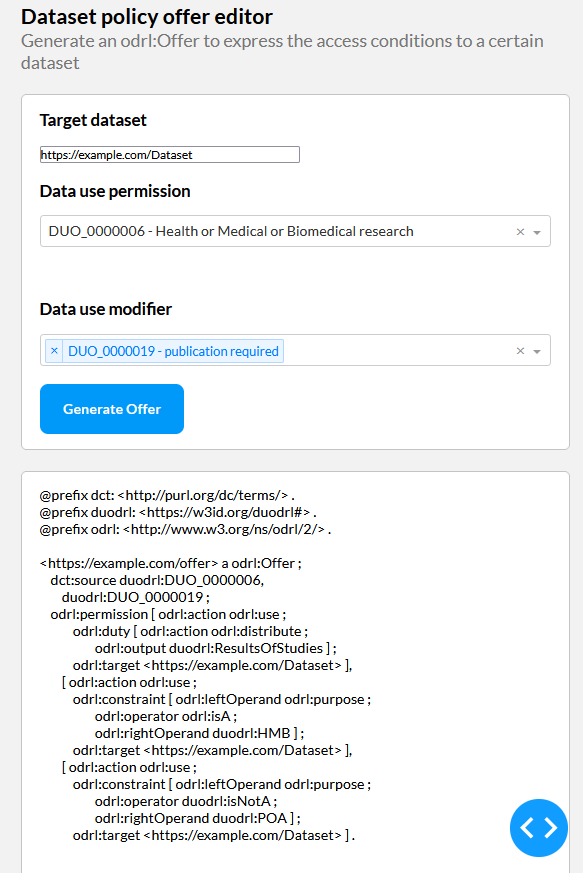
\includegraphics[width=0.4\linewidth]{figures/chapter-6/poc-editor.PNG}}
    \label{fig:editor}
}
\qquad
\subfigure[with OAC and DPV concepts.]{
    \fbox{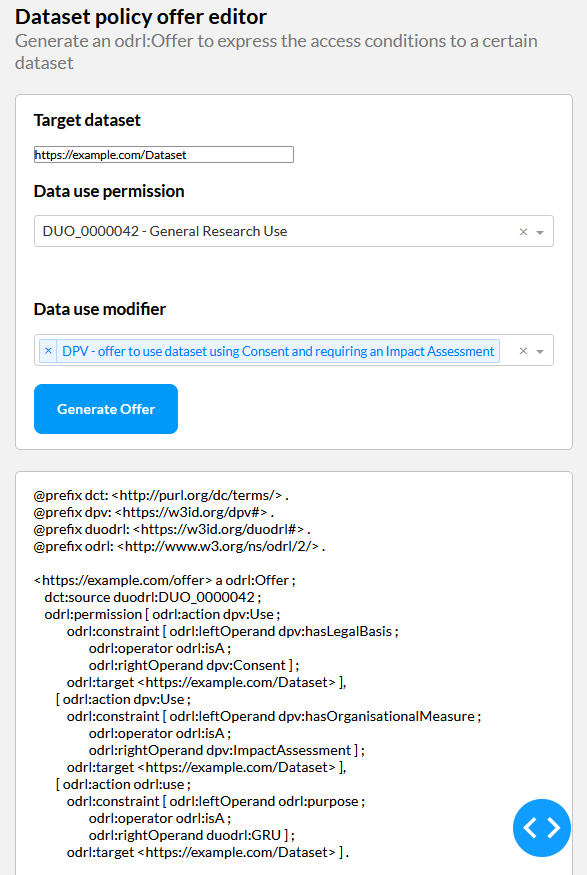
\includegraphics[width=0.4\linewidth]{figures/chapter-6/poc-dpv-editor.PNG}}
    \label{fig:dpv-editor}
}
\end{figure*}

As mentioned in the last Section, the matching algorithm employed in this PoC was adapted from the OAC-based algorithm presented in Section~\ref{sec:algorithm-agreement} to cater to DUO's use case health data-sharing conditions, while ensuring alignment with legal requirements.
During the matching process, the conditions outlined in the request for health data, in the \texttt{odrl:Request} policy, must be compared with those specified in the health datasets' offers, in the \texttt{odrl:Offer} policy.
This entails ensuring that the permissions and prohibitions from the offer instantiation can be met by the request.
Once this compatibility is established, the policies are deemed congruent, a permissive \texttt{odrl:Agreement} is generated, and access can be granted according to the established conditions.
If the policies are not compatible then a prohibitive \texttt{odrl:Agreement} is generated and access to the dataset is denied.
Moreover, for data discovery purposes, the \texttt{odrl:Request} policy needs to be compared against the policies of each available dataset if this PoC is to be implemented within a large-scale system, to ensure that all available datasets and corresponding policies are checked to see if they fit the request.
While pre-computations and optimisations could streamline this process, this is not implemented within this Thesis prototype, as its purpose is solely to serve as a first PoC to test the generation of machine and human-readable data access agreements.

The policy matching algorithm initiates by verifying if a dataset's policy includes a specific rule corresponding to the purpose outlined in the \texttt{odrl:Request}. 
If the dataset's offer has a prohibition for a purpose $P$, access to the dataset may be denied if the request is for $P$; conversely, if a permission is detected, access can be allowed allowed.
Subsequently, as described in the previous Section, similar assessments should be conducted to examine other restrictions beyond purpose, i.e., the ones outlined in Table~\ref{tab:DUO_ODRL_overview}, such as constraints on the type of assigner for the agreement, on the location or timing of data use.
In the event of encountering a matching prohibition, access to the dataset must be refused; however, if a permission is present, access may be granted.

If additional obligations are mandated for dataset access and use, such as committing to collaborate with the primary study investigator or providing proof of ethical approval to perform the study, these should included within the \texttt{odrl:Agreement} together with the conditions for access.
In instances where conflicting policies arise from the merge of distinct data use permissions and modifiers, the prohibition supersedes by default, akin to the algorithm's base protocol, established in Section~\ref{sec:algorithm}.
Under such circumstances, access to the dataset is declined.

The outcome of the matching algorithm, an \texttt{odrl:Agreement}, should be generated, incorporating a rule either permitting or prohibiting the solicited \texttt{odrl:Request}, as well as other metadata described in Section~\ref{sec:poc_duodrl}, including linkage with the corresponding \texttt{odrl:Request} and \texttt{odrl:Offer}, and any duties, if specified by the data provider.
In this way, the \texttt{odrl:Agreement} instantiation serves to encapsulate and facilitate the creation of appropriate legal documentation to formalise and communicate the agreement stemming from the submitted request and consequent matching outcome.
The computational overhead associated with generating such an agreement, particularly at a time when the request will be matched against a large number of offer policies, falls outside the scope of analysis of this Thesis.
This is due to the fact that the overhead will vary significantly depending on the use case and on the interpretation of the DUO concepts, which are not explicitly defined and, as such, reflect the specific analysis proposed in this Thesis, aligned with its core foundation on the decentralisation of access to data.
As a result, the focus of this Section is on clearly representing the information through the utilisation of ODRL policies and showcasing the applicability of the proposed OAC-based algorithm for decentralised access to health data on a purpose-based setting, aligned with the legal requirements specified in the GDPR.

%TODO: add figure with screenshot of generated agreement + human readable description

\paragraph{PoC preservation, maintenance, and future improvements}
The PoC implementation is published and archived according to the methodology described in Section~\ref{sec:code_preservation}.
Furthermore, its source code is hosted at \url{https://w3id.org/duodrl/repo}, under the CC-BY-4.0 license.
A live demonstration of the PoC UI features is also available at \url{https://w3id.org/duodrl/app}.
The repository can also be used by DUO/DUODRL users to suggest new features to be added to the PoC, as well as to report bugs through GitHub Issues.
% As future work, qSOPE can be extended to include all terms present in the previously mentioned DPV's taxonomies, as well as to cover all constraints defined in the OAC profile, e.g., restrict legal bases or specify the technical and organisational measures used by data controllers to ensure the secure processing of personal data.
% Moreover, with such an extension, SOPE could also be used by data controllers to detail their privacy policies.
% Additionally, user studies should be performed to assess the design choices included in the editor, as well as to understand what type of additional controls people want to have on top of what is legally mandated, e.g., temporal constraints or duties for the data controller to fulfil prior to data access.
% \section{Special categories of data and research exceptions}
\label{sec:biomedical_exception}

As discussed in preceding Sections, the stringent requirements for obtaining consent under the GDPR place significant burdens on data subjects.
Requiring separate agreements for each app provider and for each specific purpose leads to repetitive consent requests.
In the biomedical field, individuals may have less involvement in decision-making regarding their data compared to other sectors -- the benefits from participation in biomedical research are often not immediate and may not directly impact the individual's personal circumstances.
Consequently, individuals may be less inclined to make the effort of checking their Pod for new requests, reading information notices, and accepting/rejecting access requests, compared to sectors like information society services which include social media and streaming services.
As such, in the context of research, various provisions indicate a more flexible approach to consent requirements or even suggest moving away entirely from reliance on consent.

Recital 33 \citeyearpar{noauthor_regulation_2016} states that broad consent is permissible for research purposes under specific conditions -- \textit{``data subjects should be allowed to give their consent to certain areas of scientific research when in keeping with recognised ethical standards for scientific research''} and while having the \textit{``opportunity to give their consent only to certain areas of research or parts of research projects''}.
However, the terms `areas of research' or `parts of research projects' are domain-specific concepts that are not further defined in the GDPR.
The Global Alliance for Genomics and Health\footnote{\url{https://www.ga4gh.org/} (accessed on 9 March 2024)} develops distinct components and processes for health data sharing, including the Data Use Ontology (DUO)\footnote{\url{http://purl.obolibrary.org/obo/duo} (accessed on 9 March 2024)}, a vocabulary that can be used to describe data use conditions and limitations for research data generated in the health, clinical and biomedical domain \citep{lawson_data_2021,rehm_ga4gh_2021}.
While such vocabulary contains concepts of health-related research purposes, links to other ontologies with disease taxonomies, and incorporates concepts for modeling projects and obligations related to data usage, e.g., need for ethical approval, collaboration with the study's investigator, or the obligation to return the study's results, it does not take into consideration data protection-related requirements, e.g., legal grounds for processing.
% TODO: connect with the DUODRL chapter

However, this provision outlined in Recital 33 \citeyearpar{noauthor_regulation_2016} is not legally binding, is not mirrored in the actual text of the GDPR and it was strictly interpreted by the EDPS in its opinion on data protection and scientific research \citep{european_data_protection_supervisor_preliminary_2020}.
Furthermore, while the EDPS asserts that Recital 33 does not supersede the provisions mandating specific consent, it also suggests an assessment based on the data subject's rights, the sensitivity of the data, the nature and objective of the research, and relevant ethical safeguards. Concurrently, the EDPS also notes that if purposes cannot be precisely specified, data controllers could compensate by enhancing transparency and implementing safeguards.
Outside of the EU, the UK government advocated for an influential role for broad consent in medical research within its proposal to amend the UK's Data Protection Act \citep{uk_government_consultation_2022}.
This proposal was generally well-received, though some concerns were expressed regarding its potential for ambiguity and possible misuse.

Furthermore, the European Commission has proposed a regulation instrument for the health data domain, the European Health Data Space \citeyearpar{noauthor_proposal_2022}, which aims to depart from relying on consent for the secondary use of personal data in biomedical research.
According to this proposal, a `data holder', or a \textit{``any natural or legal person, which is an entity or a body in the health or care sector, or performing research in relation to these sectors [...] who has the right or obligation [...] to make available, including to register, provide, restrict access or exchange certain data''} \citeyearpar{noauthor_proposal_2022}, is mandated to disclose both personal and non-personal data under specific conditions and for a limited set of purposes, including scientific research (Article 34.1(e) \citeyearpar{noauthor_proposal_2022}), without requiring the consent of the data subject.
Additionally, Article 33.5 of the EHDS proposal \citeyearpar{noauthor_proposal_2022} appears to override national laws mandating consent by stipulating that \textit{``where the consent of the natural person is required by national law, health data access bodies shall rely on the obligations laid down in this Chapter to provide access to electronic health data''}.
The final version of this proposal, including the role of consent and its scope (broad or specific), is yet to be determined.
However, this proposal has drawn criticism from both the EDPB and EDPS in a joint opinion document, which calls for further clarification on how national laws requiring consent will interact with the proposed European legislation \citeyearpar{noauthor_edpbedps_2022}.

Biomedical research presents challenges within the GDPR due to its unique combination of a stringent regulatory framework, as it involves processing health data, which falls under the GDPR's special categories of data, alongside a set of exemptions designed to facilitate research due to its societal significance.

\subsection{A stricter regime for health data processing}
\label{sec:stricter_regime}

GDPR's Article 9.1 \citeyearpar{noauthor_regulation_2016} prohibits the processing of special categories of data, including health data.
However, there are ten exceptions to this rule, one of which is explicit consent from the data subject.
Nevertheless, the term `explicit' lacks clarity, as it's unclear what distinguishes it from `regular' consent, which requires a clear affirmative action or statement by the data subject.
Further clarification is needed in the GDPR regarding the additional steps a controller should take to obtain explicit consent from a data subject \citep{european_data_protection_board_guidelines_2020}.
The EDPB offers various examples of how explicit consent can be expressed.
These include providing a written statement, or in the digital context, actions such as filling out an electronic form, sending an email, uploading a scanned document bearing the data subject's signature, or using an electronic signature.
Another method mentioned is two-stage verification, where the data subject may receive an email from the controller requesting consent to process specific medical data.
Upon agreement, the data subject is asked to respond via email with the phrase `I agree', followed by receiving a verification link or an SMS message for confirmation \citep{european_data_protection_board_guidelines_2020}.

Within decentralised frameworks such as Solid, various approaches can be employed for the purpose of expressing explicit consent.
Depending on the Solid server chosen by users to host their Pod, an inbox container, akin to email inboxes found in other systems, may be automatically created when the user sets up the Pod.
This container can serve as a platform to receive such requests as it is equipped with a specialised access control authorisation, allowing only the data subject to read its contents while permitting other users to write to it. 
However, due to the lack of standardisation across the Solid ecosystem, the presence of this container cannot always be guaranteed, or it may be named differently, leading to interoperability issues.
A more sophisticated solution involves adopting a graph-centric interpretation of a Pod, wherein each Solid Pod functions as a hybrid, contextualised knowledge graph \citep{dedecker_whats_2022}.
In this context, `hybrid' denotes support for both documents and RDF statements, while `contextualised' signifies the ability to associate each document and statement with metadata such as policies or provenance data.
By accurately recording metadata, including context and provenance, multiple interfaces of the Pod can be generated as needed by various applications chosen by the data subject.
In this scenario, requests can be seamlessly integrated into the graph without requiring hardcoded specifications in the application for where the requests should be written.
These requests can then be visualised by the data subject using a Solid application or service compatible with this graph-centric approach.
Additionally, the research conducted by \cite{braun_selfverifying_2022} can be utilised to sign and validate resources carrying the `I agree' statement of the data subject.

In summary, expressing explicit consent through pre-set polices poses challenges.
Matching user policies, predefined in advance, with data requests is unlikely to meet the explicit nature of consent. 
Although matching can enhance transparency and assist individuals in decision-making, a separate action of explicitly approving the use of personal data is required to meet the explicit requirement of consent.

\subsection{A series of derogations for research purposes}
\label{sec:derogations}

In this Section, three distinct aspects, relevant to the domain of health research, are discussed: (i) the compatibility between data collection purposes and secondary reuse for research, (ii) exceptions from the right to information, and (iii) alternative exceptions, aside from consent, for processing special categories of data.

\paragraph{Secondary use for research}
As previously discussed in Section \ref{sec:consent_compatibility}, related to the `purpose limitation' principle and the assessment of compatibility, the GDPR states that \textit{``data shall be collected for specific, explicit and legitimate purposes and not further processed in a manner that is incompatible with those purposes''} (Article 5.1(b) \citeyearpar{noauthor_regulation_2016}).
As such, there is an assumption of compatibility between the purpose of collection and subsequent reuse, provided that the personal data processing for scientific research purposes appropriately implements safeguards to protect the rights and freedoms of the data subject (as outlined in Article 89.1 \citeyearpar{noauthor_regulation_2016}).
It is crucial to highlight that the prohibition against processing personal data for incompatible purposes differs from the requirement of purpose specificity, and an exception does not alleviate the need for a specific purpose.
Moreover, regardless of compatibility, the data controller must rely on consent or another legal ground to process personal (health) data.
However, there is one provision in the GDPR preamble that questions the distinction between these two requirements -- \textit{``The processing of personal data for purposes other than those for which the personal data were initially collected should be allowed only where the processing is compatible with the purposes for which the personal data were initially collected. In such a case, no legal basis separate from that which allows the collection of the personal data is required''} (Recital 50 \citeyearpar{noauthor_regulation_2016}).
This appears to challenge the separation between the `purpose limitation' and the `lawfulness' principles.
This intersection, and its implications for decentralised data-sharing ecosystems such as Solid, needs to be further investigated.

\paragraph{Exceptions to the information obligations}
In Section \ref{sec:specific_consent}, particularly in the ``Identifying the data controller'' paragraph, the information obligations outlined in Articles 13 and 14 of the GDPR \citeyearpar{noauthor_regulation_2016} are explored, with a focus on the timing of when information must be provided to the data subject.
In particular, Article 14 provides an exception for cases where personal data are processed for research purposes and have not been obtained directly from the data subject.
This exception may be relevant to Solid, considering that not all personal data stored in Solid Pods originates directly from the data subject -- it may be generated by app providers, Pod providers, other users, or agents.
Furthermore, according to Article 14.5, if (i) providing information is impossible or would require disproportionate effort, or if doing so is likely to render impossible or seriously impair the achievement of the processing objectives, and (ii) the conditions and safeguards specified in Article 89 \citeyearpar{noauthor_regulation_2016} are met, the information requirements outlined in Article 14 are inapplicable.
The compliance of Solid-based data exchanges with these conditions and safeguards in place will need to be evaluated on a case-by-case basis, depending on the context and the data access request.
However, it is probable that these conditions will be fulfilled only in exceptional cases rather than as a standard practice, and if they are met, the data controller \textit{``shall take appropriate measures to protect the data subject's rights and freedoms and legitimate interests, including making the information publicly available''}. 
As such, further research is needed to explore the role of Solid's notification system, as well as other mechanisms, to act as appropriate measures to safeguard the rights of the data subject.

\paragraph{Alternative legal bases beyond consent}
In addition to explicit consent, GDPR's Article 9.2 \citeyearpar{noauthor_regulation_2016} outlines other exceptions to the prohibition on processing special categories of data.
Article 9.2(j) is particularly pertinent to this discussion because it pertains to the processing of personal data for health research.
This point permits the processing of health-related data when it is necessary for scientific research in accordance with Article 89.1 \citeyearpar{noauthor_regulation_2016}, as long as it is based on European or national law.
Such processing must be proportionate to the intended purpose, uphold the essence of the right to data protection, and include appropriate and specific measures to safeguard the fundamental rights and interests of the data subject.
Consequently, the applicability of this exception hinges on the identification of a European or national law that can justify the processing of personal data.
If the processing falls within the scope of such legislation, explicit consent from the data subject is not required.

As such, from this Section is possible to conclude that the exemptions for processing personal data for scientific research hinge on the adoption and use of suitable safeguards.
According to GDPR's Article 89.1, these safeguards center around upholding the `data minimisation' principle and include practices like pseudonymisation and methods that prevent the identification of data subjects.
Subsequent research could explore whether PIMS, such as the Solid with an OAC-based matching system, could serve as a safeguard in this context.


% \section{Ethical challenges of controlling data and reclaiming control over it}
\label{sec:ethical_challenges}

Advancements in data-driven innovations are poised to drive further economic and societal progress \citep{jacobides_platforms_2019}.
The analysis, sharing, and reuse of data have led to transformative changes in business models and government processes, enabling them to capitalise on these practices. 
As discussed in the previous Sections, these changes propelled policy initiatives implemented by various governments globally.
In particular, the EU is actively engaged in this transformation, exemplified by the \cite{european_commission_communication_2020} commitment\footnote{The European Commission's strategy and related documents are available at \url{https://ec.europa.eu/info/strategy/priorities-2019-2024/europe-fit-digital-age_en} (accessed on 10 March 2024)} to shaping ``A Europe fit for the Digital Age''. 
Whether it is a prominent Big Tech firm headquartered in the United States, a major data intermediary in the EU, or a state-controlled entity in China, contemporary data practices face scrutiny from diverse sectors of society, spanning individuals, non-governmental organisations (NGOs), academics, and governmental bodies.
Such distrust in digital services has been called into question \citep{waldman_industry_2021}, prompting individuals to ponder who should they trust their data with.

Amidst this trust crisis, technology has emerged as a potential solution, in particular self-sovereign PIMS \citep{chomczyk_penedo_selfsovereign_2021}, as discussed in Section~\ref{sec:motivation_legal}.
These models empower users to directly control their data, dictating the terms of access and usage, and have been gaining the support of policymakers, in particular in Europe, with the European Commission supporting the creation of common European data spaces \citeyearpar{noauthor_commission_2022}.
Moreover, it could be argued that the EU is strategically investing in these technologies to foster more democratic and participatory data practices, and enhance confidence in data-intensive operations by advocating for technologically robust systems that reduce reliance on the reputation of individual firms, thus mitigating power imbalances between data subjects and controllers \citep{european_commission_communication_2020}.

The literature exploring the concept of trust is extensive, yet complex due to varying interpretations.
\cite{de_filippi_blockchain_2020} distinguished trust from confidence, noting that trust is rooted in personal vulnerability and risk-taking, while confidence is based on internalised expectations stemming from knowledge or past experiences.
As such, in this Section, the interest of data subjects in technologies that provide insights into how their information is integrated into real personal data handling processes is studied as a vehicle of trust, given their general apprehension regarding the processing actions of data controllers over personal data.
As visible in the previous Sections, the personal data regulatory framework in the EU is designed to address imbalances or vulnerabilities between multiple parties by revealing potential risks and resulting harms, aiming to leverage consent as a catalyst for the data-driven economy \citep{chomczyk_penedo_towards_2022}. 
Simultaneously, they aim to furnish essential information to individuals making decisions, facilitating informed choices \cite{benshahar_more_2014}.
Furthermore, from an ethical standpoint, several norms emerge that should guide the conduct of individuals with whom information is shared to ensure trustworthiness.
These norms encompass sincerity, competence, and the appropriateness of the entrusted task \citep{hawley_how_2019}.

Considering the myriad of factors influencing both trust and confidence, the analysis in this Section focuses on (i) transparency as a crucial prerequisite for the functioning of decentralised PIMS, (ii) the relevant EU regulatory framework on personal data, and (iii) an ethical debate concerning data control, as outlined in \citeauthor{bodo_mediated_2021}'s framework for mediated technological trust.
The emphasis on transparency stems from three primary considerations:
\begin{itemize}
    \item from a regulatory viewpoint, transparency stands as a fundamental principle within personal data protection regimes, often integrated alongside lawfulness and fairness, as exemplified in GDPR's Article 5.1(a);
    \item transparency encompasses both its \textit{ex-ante} and \textit{ex-post} components, with the latter including the issue of explainability \citep{felzmann_transparency_2019};
    \item transparency offers the potential to demystify the `black box' nature of many AI systems, enabling the identification of potential biases towards vulnerable populations \citep{pasquale_black_2015}.
\end{itemize}

As illustrated by case law from supervisory authorities, the intricate nature of data processing activities has proven challenging for data controllers to articulate in straightforward terms, especially when relying on limited attention resources from data subjects \citep{european_data_protection_board_guidelines_2020}.
The dearth of actionable information, to understand data handling practices, poses a risk to fostering trust among involved parties.
As a result, individuals are endeavoring to reassert control over their data and restrict its usage by such entities, also by looking at new data governance schemes such as PIMS or other data intermediaries \citep{craglia_digitranscope_2021,papagiannakopoulou_leveraging_2014}. 

As such, the concept of `control' gains particular importance as users require someone to trust in order to reclaim control over their data in the digital era.
Emerging data governance models are coupled with legal frameworks to assist data subjects in asserting their agency.
For instance, in the data cooperative model (which is regulated by the DGA), cooperatives act as trustees overseeing data on behalf of data subjects, thus enabling data subjects to maintain democratic control over their data. 
In such governance frameworks, establishing a relationship of trust between cooperatives managing data and data subjects is paramount.
In certain instances, trustees may need to consult with data subjects, providing agreements and contracts to inform them. 
Meanwhile, data subjects can articulate their preferences and determine how to share their data and for what purposes \citep{craglia_digitranscope_2021}.

Data cooperatives and other intermediaries (will) play a pivotal role in empowering data subjects to maintain control over their data and reassert their ethical standing in the digital era.
Specifically, personal data sovereignty offers a significant return to more democratic and egalitarian governance, allowing individuals to reclaim control over their personal data \citep{craglia_digitranscope_2021, giannopoulou_digital_2023}.
In theory, these systems should restore personal autonomy and uphold classical liberal values by fostering trust-based relationships. %TODO: add citation
Furthermore, drawing from our current democratic experiences can offer valuable lessons to avoid repeating the same mistakes made in the past two centuries.
During this time, a substantial portion of the population, particularly in the Global South, suffered from neglected rights due to inadequate governance safeguards. %TODO: add citation
For instance, democratic failures in Latin America over the last 50 years, stemming from regime changes, economic crises, or environmental catastrophes, have led to the absence of robust governance mechanisms to address such challenges.
One illustrative example is the impact of the last Argentinian military dictatorship, which significantly altered the identities of numerous individuals who were abducted as children and placed with new families, effectively erasing their true identities.
In response, collective organisations emerged to address this injustice, recognising the vulnerable position these individuals were placed in and their limited ability to resist and reclaim their true identities \citep{gesteira_mas_2014}.

Despite the critical role of trust in upholding the autonomy and agency of data subjects \citep{benshahar_more_2014}, the methods currently employed to foster trust remain contentious, and unresolved societal issues persist in digital services and emerging digital intermediaries \citep{carovano_regulating_2023}.
Given the practical nature of the issues at hand, including how to practically approach trust, establish trust relationships between data subjects and data intermediaries, and identify the necessary conditions for fostering trust, a public Think-In event was organised in the context of the PROTECT project.
In these events, individuals were convened to explore the implications of governing personal data spaces through decentralised PIMS or trusted data intermediaries.
With the ``citizens' Think-In'' approach, there is a public discussion focused on the opinion of individuals, which encourages direct participation from attendees.
In particular, through small-scale group discussions, a Think-In offers a platform for individuals from diverse backgrounds to deliberate and exchange views on current societal issues stemming from advancements in Science, Technology, Engineering, and Mathematics (STEM) fields\footnote{Information regarding the organised PROTECT Think-Ins and respective results is available at \url{https://protect.oeg.fi.upm.es/thinkin/} (accessed on 11 March 2024)}. %TODO: add citation of think-ins

While the comprehensive outcomes of the Think-In process will not be included in this Thesis as a contribution, it is worth noting that the general public exhibited sensitivity toward the ethical considerations regarding whom to trust and the significance of transparency in such contexts.
Citizens emphasised the importance of preventing the GDPR from turning into a mere `tick-box' compliance exercise, similar to the current format of privacy notices which result from deploying template privacy notices for distinct data processing activities.
Furthermore, there was a call for increased disclosure and oversight concerning the practical and beneficial utilisation of personal data, highlighting the importance of meaningful transparency in fostering trust among parties involved in such sensitive data exchanges.

To conclude, the insights derived from the Citizens' Think-In discussion offer a valuable foundation for considering the integration of transparency into data access agreement terms for personal data vaults, presented in both machine-readable and human-readable formats.
This approach enables data subjects to better comprehend and manage the expression of policy terms, and empowers data controllers and data subjects to navigate the intricate data-sharing landscape of the platform economy with greater control vested in the subject.



% Design and implementation of a policy matching algorithm and data-sharing agreement generator prototype for access to data stored in Solid Pods.
\chapter{Going beyond the GDPR -- Exploring the Data Governance Act}
\label{chap:dga}

\begin{tcolorbox}[colback=royallavender!40]
The content of this Chapter has already been partially included in the articles published during this Thesis % \citep{esteves_fostering_2022,asgarinia_who_2023,florea_is_2023}. TODO: cite semantics poster, DGA paper and soda demo paper
\end{tcolorbox}

% This Chapter discusses the legal and ethical challenges of the impact of data-driven innovation in society, in particular, related to the emergence of PIMS as a service that helps individuals have more control over the processing of their data.
% While some studies have recently been published on the intersection of Solid and data protection requirements, as reviewed in Section~\ref{sec:sota_solid_data_protection}, plenty still has to be overcome to have a `legally-aligned' personal datastore.
% This interdisciplinary discussion relies on the collaborations fostered through the PROTECT project, and other EU-funded projects described in Section~\ref{sec:projects}, as well as through the participation in the W3C DPVCG work with data protection law experts.
% 
% Section~\ref{sec:motivation_legal} describes the emergence of decentralised personal information management systems as a way to give users more control over their personal data and the challenges that still need to be overcome in order to have to a GDPR-aligned personal datastore.
% 
% Section~\ref{sec:policies_consent} discusses the usage of OAC policies as a precursor of consent for Solid, which can enable compliance with several GDPR requirements including the transparent information obligations of Articles 13 and 14 and the conditions to obtain valid consent pursuant to Articles 4.11 and 7.
% 
% Section~\ref{sec:automation_consent} argues whether the automation of consent can be performed while maintaining the `informed', `freely given', `specific', and `unambiguous' character of GDPR consent.
% In particular, the specificity of purposes and processing operations, the distinction between data controllers and recipients, the compatibility of purposes, and the delegation of consent are further analysed through a `legal+tech' approach, relying on GDPR's requirements and on the OAC and PLASMA implementations.
% 
% Section~\ref{sec:biomedical_exception} discusses the special requirements of GDPR's special categories of data and research-related exceptions and, in particular, the requirements related to the sharing of health data for biomedical research or for the management of public health.
% 
% To conclude, Section~\ref{sec:ethical_challenges} debates the ethical challenges of controlling data and reclaiming control over it and explores how decentralised PIMS can help build confidence in data exchange practices and trust in the providers and developers of such systems.

\section{Information flows in the DGA}
\label{sec:dga_flows}

Figure of information flows and documents (from the paper)
Comparison with GDPR flows
Identification of important use cases that can be tackled and easily extended with the work already developed for GDPR
\section{DGAterms}
\label{sec:dgaterms}

As an active contributor in the realm of data protection, the Semantic Web community possesses significant potential to aid with the compliance processes that such a legislation involve.
Such potential is based on the opportunities for interoperability that such a Web of Linked Data can support.
In this context, Semantic Web technologies can be utilised:
\begin{itemize}
    \item to model conditions for the reuse of public data;
    \item by data subjects, data holders and data users to declare data access and usage policies in a machine-readable format; and
    \item by organisations and service providers to maintain records of the processing activities.
\end{itemize}

% requirements specification -- ORSD
% vocab implementation details
% Vocabulary publication and maintenance
% vocab evaluation
\section{Lessons learned for the (Personal) Data Spaces future}
\label{sec:dgaterms}

contributions towards the EHDS
% \input{mainmatter/5_legal/5-4_biomedical_exceptiosn}
% \section{Ethical challenges of controlling data and reclaiming control over it}
\label{sec:ethical_challenges}

Advancements in data-driven innovations are poised to drive further economic and societal progress \citep{jacobides_platforms_2019}.
The analysis, sharing, and reuse of data have led to transformative changes in business models and government processes, enabling them to capitalise on these practices. 
As discussed in the previous Sections, these changes propelled policy initiatives implemented by various governments globally.
In particular, the EU is actively engaged in this transformation, exemplified by the \cite{european_commission_communication_2020} commitment\footnote{The European Commission's strategy and related documents are available at \url{https://ec.europa.eu/info/strategy/priorities-2019-2024/europe-fit-digital-age_en} (accessed on 10 March 2024)} to shaping ``A Europe fit for the Digital Age''. 
Whether it is a prominent Big Tech firm headquartered in the United States, a major data intermediary in the EU, or a state-controlled entity in China, contemporary data practices face scrutiny from diverse sectors of society, spanning individuals, non-governmental organisations (NGOs), academics, and governmental bodies.
Such distrust in digital services has been called into question \citep{waldman_industry_2021}, prompting individuals to ponder who should they trust their data with.

Amidst this trust crisis, technology has emerged as a potential solution, in particular self-sovereign PIMS \citep{chomczyk_penedo_selfsovereign_2021}, as discussed in Section~\ref{sec:motivation_legal}.
These models empower users to directly control their data, dictating the terms of access and usage, and have been gaining the support of policymakers, in particular in Europe, with the European Commission supporting the creation of common European data spaces \citeyearpar{noauthor_commission_2022}.
Moreover, it could be argued that the EU is strategically investing in these technologies to foster more democratic and participatory data practices, and enhance confidence in data-intensive operations by advocating for technologically robust systems that reduce reliance on the reputation of individual firms, thus mitigating power imbalances between data subjects and controllers \citep{european_commission_communication_2020}.

The literature exploring the concept of trust is extensive, yet complex due to varying interpretations.
\cite{de_filippi_blockchain_2020} distinguished trust from confidence, noting that trust is rooted in personal vulnerability and risk-taking, while confidence is based on internalised expectations stemming from knowledge or past experiences.
As such, in this Section, the interest of data subjects in technologies that provide insights into how their information is integrated into real personal data handling processes is studied as a vehicle of trust, given their general apprehension regarding the processing actions of data controllers over personal data.
As visible in the previous Sections, the personal data regulatory framework in the EU is designed to address imbalances or vulnerabilities between multiple parties by revealing potential risks and resulting harms, aiming to leverage consent as a catalyst for the data-driven economy \citep{chomczyk_penedo_towards_2022}. 
Simultaneously, they aim to furnish essential information to individuals making decisions, facilitating informed choices \cite{benshahar_more_2014}.
Furthermore, from an ethical standpoint, several norms emerge that should guide the conduct of individuals with whom information is shared to ensure trustworthiness.
These norms encompass sincerity, competence, and the appropriateness of the entrusted task \citep{hawley_how_2019}.

Considering the myriad of factors influencing both trust and confidence, the analysis in this Section focuses on (i) transparency as a crucial prerequisite for the functioning of decentralised PIMS, (ii) the relevant EU regulatory framework on personal data, and (iii) an ethical debate concerning data control, as outlined in \citeauthor{bodo_mediated_2021}'s framework for mediated technological trust.
The emphasis on transparency stems from three primary considerations:
\begin{itemize}
    \item from a regulatory viewpoint, transparency stands as a fundamental principle within personal data protection regimes, often integrated alongside lawfulness and fairness, as exemplified in GDPR's Article 5.1(a);
    \item transparency encompasses both its \textit{ex-ante} and \textit{ex-post} components, with the latter including the issue of explainability \citep{felzmann_transparency_2019};
    \item transparency offers the potential to demystify the `black box' nature of many AI systems, enabling the identification of potential biases towards vulnerable populations \citep{pasquale_black_2015}.
\end{itemize}

As illustrated by case law from supervisory authorities, the intricate nature of data processing activities has proven challenging for data controllers to articulate in straightforward terms, especially when relying on limited attention resources from data subjects \citep{european_data_protection_board_guidelines_2020}.
The dearth of actionable information, to understand data handling practices, poses a risk to fostering trust among involved parties.
As a result, individuals are endeavoring to reassert control over their data and restrict its usage by such entities, also by looking at new data governance schemes such as PIMS or other data intermediaries \citep{craglia_digitranscope_2021,papagiannakopoulou_leveraging_2014}. 

As such, the concept of `control' gains particular importance as users require someone to trust in order to reclaim control over their data in the digital era.
Emerging data governance models are coupled with legal frameworks to assist data subjects in asserting their agency.
For instance, in the data cooperative model (which is regulated by the DGA), cooperatives act as trustees overseeing data on behalf of data subjects, thus enabling data subjects to maintain democratic control over their data. 
In such governance frameworks, establishing a relationship of trust between cooperatives managing data and data subjects is paramount.
In certain instances, trustees may need to consult with data subjects, providing agreements and contracts to inform them. 
Meanwhile, data subjects can articulate their preferences and determine how to share their data and for what purposes \citep{craglia_digitranscope_2021}.

Data cooperatives and other intermediaries (will) play a pivotal role in empowering data subjects to maintain control over their data and reassert their ethical standing in the digital era.
Specifically, personal data sovereignty offers a significant return to more democratic and egalitarian governance, allowing individuals to reclaim control over their personal data \citep{craglia_digitranscope_2021, giannopoulou_digital_2023}.
In theory, these systems should restore personal autonomy and uphold classical liberal values by fostering trust-based relationships. %TODO: add citation
Furthermore, drawing from our current democratic experiences can offer valuable lessons to avoid repeating the same mistakes made in the past two centuries.
During this time, a substantial portion of the population, particularly in the Global South, suffered from neglected rights due to inadequate governance safeguards. %TODO: add citation
For instance, democratic failures in Latin America over the last 50 years, stemming from regime changes, economic crises, or environmental catastrophes, have led to the absence of robust governance mechanisms to address such challenges.
One illustrative example is the impact of the last Argentinian military dictatorship, which significantly altered the identities of numerous individuals who were abducted as children and placed with new families, effectively erasing their true identities.
In response, collective organisations emerged to address this injustice, recognising the vulnerable position these individuals were placed in and their limited ability to resist and reclaim their true identities \citep{gesteira_mas_2014}.

Despite the critical role of trust in upholding the autonomy and agency of data subjects \citep{benshahar_more_2014}, the methods currently employed to foster trust remain contentious, and unresolved societal issues persist in digital services and emerging digital intermediaries \citep{carovano_regulating_2023}.
Given the practical nature of the issues at hand, including how to practically approach trust, establish trust relationships between data subjects and data intermediaries, and identify the necessary conditions for fostering trust, a public Think-In event was organised in the context of the PROTECT project.
In these events, individuals were convened to explore the implications of governing personal data spaces through decentralised PIMS or trusted data intermediaries.
With the ``citizens' Think-In'' approach, there is a public discussion focused on the opinion of individuals, which encourages direct participation from attendees.
In particular, through small-scale group discussions, a Think-In offers a platform for individuals from diverse backgrounds to deliberate and exchange views on current societal issues stemming from advancements in Science, Technology, Engineering, and Mathematics (STEM) fields\footnote{Information regarding the organised PROTECT Think-Ins and respective results is available at \url{https://protect.oeg.fi.upm.es/thinkin/} (accessed on 11 March 2024)}. %TODO: add citation of think-ins

While the comprehensive outcomes of the Think-In process will not be included in this Thesis as a contribution, it is worth noting that the general public exhibited sensitivity toward the ethical considerations regarding whom to trust and the significance of transparency in such contexts.
Citizens emphasised the importance of preventing the GDPR from turning into a mere `tick-box' compliance exercise, similar to the current format of privacy notices which result from deploying template privacy notices for distinct data processing activities.
Furthermore, there was a call for increased disclosure and oversight concerning the practical and beneficial utilisation of personal data, highlighting the importance of meaningful transparency in fostering trust among parties involved in such sensitive data exchanges.

To conclude, the insights derived from the Citizens' Think-In discussion offer a valuable foundation for considering the integration of transparency into data access agreement terms for personal data vaults, presented in both machine-readable and human-readable formats.
This approach enables data subjects to better comprehend and manage the expression of policy terms, and empowers data controllers and data subjects to navigate the intricate data-sharing landscape of the platform economy with greater control vested in the subject.



% How can OAC be extended to create DGA-aligned policies
% Development of a Data Governance Act (DGA) vocabulary, to create OAC-based policies for the sharing of data for altruistic purposes and keep registries of available datasets.

\part{CONCLUSIONS}

\chapter{Conclusions}
\label{chap:conclusions}

In a world where AI-based technologies are taking over and distrust in data-consuming services is at its highest point in today's Web, BigTech companies prefer to deal with the consequences of their unlawful practices than provide the necessary tools to data subjects to make the right decisions over the processing of their personal data.
Endowed with enhanced interoperability and transparency features, the decentralised Semantic Web aims to aid data subjects in taking control of the publication and movement of their personal data.
As such, legally-aligned vocabularies and services were produced to support policy-based access to data in decentralised settings, providing accountability and enhanced transparency to people looking at regaining trust in Web services. 
To this end, Section~\ref{sec:fulfilment} concludes the Thesis with a discussion on the extent to which the research objectives have been fulfilled through the contributions described in Chapters~\ref{chap:vocabularies} to~\ref{chap:dga}.
Finally, Section~\ref{sec:future_work} provides lines of future work arising from the research presented within this Thesis.

\section{Fulfilment of research objectives}
\label{sec:fulfilment}
\section{Future work}
\label{sec:future_work}

With the European Commission expanding the scope of its legislative initiatives from personal data, to non-personal data and to the under-development common European data spaces, further opportunities for future work based on the contributions proposed in this Thesis can be envisioned.

\paragraph{Beyond consent} The contributions proposed in this Thesis focus on the usage of consent as the legal basis for the processing of personal data. This places a lot of responsibilities on the data subject, which would need to individually approve every request for data. To avoid consent fatigue, other GDPR legal bases, described in Article 6~\citeyearpar{noauthor_regulation_2016}, should also be used by data controllers for the lawful processing of personal data, in particular the usage of contracts or legitimate interests.

\paragraph{Delegation and data reuse} The central theme of this Thesis revolves around empowering data subjects to exert control over the fate of their data. However, there are situations where data subjects might want to rely on other people or organisations to make the decisions for them. A first step was taken by the work on DGAterms, which can be used by data subjects to specify under which conditions their data is available, and in turn intermediation service providers and altruistic organisations make it available to data users, following these conditions. This work should be expanded to cover a wider set of use cases, e.g., allow data subjects to delegate the decision of what happens with their health data to their doctor. Moreover, the EHDS proposal~\citeyearpar{noauthor_proposal_2022} expands on DGA's altruistic intentions by providing an extensive set of altruistic purposes for the secondary use of data for improved healthcare services or innovative research on rare diseases.

\paragraph{Usage control and data spaces} While this Thesis focused on building solutions to aid data subjects and data controllers in dealing with access to data, the envisioned European data spaces are putting the focus on usage control solutions. As proven by the work on DUODRL, the proposed vocabularies can be easily extended to include usage constraints, e.g., publishing the results of the research, and the proposed architecture should be developed to include a usage control enforcement component.

\paragraph{Web agents} Building on the previous three points, decentralised data environments such as Solid can rely on Web agents to assist data subjects, data controllers, and newly-introduced DGA entities to exercise their rights or fulfil their duties in an automated manner. In this context, agents can be useful in making decisions for the data subjects, according to their preferences, help data controllers to compile the necessary compliance documentation, or aid altruistic organisations in their data meddling functions.

\paragraph{More privacy interfaces} This Thesis showcases three proof of concept user interfaces for data subjects to edit their privacy preferences and exercise their right of access. These interfaces should be further improved to cover a wider range of policies, as well as to enclose tools to assist data subjects in the exercise of all of their GDPR data subjects and further rights from other European and non-European laws. Moreover, privacy dashboards for users to manage their data and understand how it is being used and by whom should also be developed.

\paragraph{Contextualised and verifiable data} As described by~\cite{verborgh_rawdata_2023}, \textit{``Data without context is meaningless; data without trust is useless.''} When data subjects give access to their data, they want to know that it is going to be used according to their preferences and not for purposes that they do not agreed with. On the other hand, data controllers and data users want to know that they are receiving complete and correct data, while supervisory authorities need to have access to contextualised data access and usage metadata to verify that it is not being misused. As such, to have trustful and responsible data flows in decentralised data environments, data should be accessed and shared with accompanying access and usage policies as well as contextual metadata and digital signatures.

\paragraph{Interaction of data protection and AI laws} Beyond GDPR and the DGA, the European strategy for data also introduced the Digital Services Act (DSA)~\citeyearpar{noauthor_dsa_2022}, the Digital Markets Act (DMA)~\citeyearpar{noauthor_dma_2022}, and the Data Act~\citeyearpar{noauthor_dataact_2022} legislative initiatives. Moreover, the EC also launched the first-ever legal framework on AI, the AI Act~\citeyearpar{noauthor_proposal_2021}.
Additionally, the rest of the world is following the European approach, with new data and AI-related legal frameworks being launched outside the EU. To deal with the new requirements brought on by these new laws, further vocabularies need to be developed and integrated into DPV's existing framework, which currently covers jurisdiction-agnostic as well as GDPR and DGA-specific terms. Furthermore, a study of how these laws are related and in which data processing scenarios they apply still needs to be performed to be incorporated into the developed decentralised systems.

\cleardoublepage

% --------------------------
% Back matter
% --------------------------
\backmatter
% \printbibliography[title=Referencias, heading=bibintoc]
\bibliography{thesisRefs}

%\appendix
%\chapter{Annexes}  

% **************************************************
% End of document
% **************************************************
\end{document}
